\documentclass[]{book}
\usepackage{lmodern}
\usepackage{amssymb,amsmath}
\usepackage{ifxetex,ifluatex}
\usepackage{fixltx2e} % provides \textsubscript
\ifnum 0\ifxetex 1\fi\ifluatex 1\fi=0 % if pdftex
  \usepackage[T1]{fontenc}
  \usepackage[utf8]{inputenc}
\else % if luatex or xelatex
  \ifxetex
    \usepackage{mathspec}
  \else
    \usepackage{fontspec}
  \fi
  \defaultfontfeatures{Ligatures=TeX,Scale=MatchLowercase}
\fi
% use upquote if available, for straight quotes in verbatim environments
\IfFileExists{upquote.sty}{\usepackage{upquote}}{}
% use microtype if available
\IfFileExists{microtype.sty}{%
\usepackage{microtype}
\UseMicrotypeSet[protrusion]{basicmath} % disable protrusion for tt fonts
}{}
\usepackage[margin=1in]{geometry}
\usepackage{hyperref}
\hypersetup{unicode=true,
            pdftitle={A Text For SCI200\\Genetics at Roxbury Community College},
            pdfauthor={Nikolaus Sucher},
            pdfborder={0 0 0},
            breaklinks=true}
\urlstyle{same}  % don't use monospace font for urls
\usepackage{longtable,booktabs}
\usepackage{graphicx,grffile}
\makeatletter
\def\maxwidth{\ifdim\Gin@nat@width>\linewidth\linewidth\else\Gin@nat@width\fi}
\def\maxheight{\ifdim\Gin@nat@height>\textheight\textheight\else\Gin@nat@height\fi}
\makeatother
% Scale images if necessary, so that they will not overflow the page
% margins by default, and it is still possible to overwrite the defaults
% using explicit options in \includegraphics[width, height, ...]{}
\setkeys{Gin}{width=\maxwidth,height=\maxheight,keepaspectratio}
\IfFileExists{parskip.sty}{%
\usepackage{parskip}
}{% else
\setlength{\parindent}{0pt}
\setlength{\parskip}{6pt plus 2pt minus 1pt}
}
\setlength{\emergencystretch}{3em}  % prevent overfull lines
\providecommand{\tightlist}{%
  \setlength{\itemsep}{0pt}\setlength{\parskip}{0pt}}
\setcounter{secnumdepth}{5}
% Redefines (sub)paragraphs to behave more like sections
\ifx\paragraph\undefined\else
\let\oldparagraph\paragraph
\renewcommand{\paragraph}[1]{\oldparagraph{#1}\mbox{}}
\fi
\ifx\subparagraph\undefined\else
\let\oldsubparagraph\subparagraph
\renewcommand{\subparagraph}[1]{\oldsubparagraph{#1}\mbox{}}
\fi

%%% Use protect on footnotes to avoid problems with footnotes in titles
\let\rmarkdownfootnote\footnote%
\def\footnote{\protect\rmarkdownfootnote}

%%% Change title format to be more compact
\usepackage{titling}

% Create subtitle command for use in maketitle
\newcommand{\subtitle}[1]{
  \posttitle{
    \begin{center}\large#1\end{center}
    }
}

\setlength{\droptitle}{-2em}
  \title{A Text For SCI200
  \\ Genetics at Roxbury Community College}
  \pretitle{\vspace{\droptitle}\centering\huge}
  \posttitle{\par}
  \author{Nikolaus Sucher}
  \preauthor{\centering\large\emph}
  \postauthor{\par}
  \date{}
  \predate{}\postdate{}

\usepackage{geometry}
\usepackage{fontspec}
%\setmainfont{Lucida Grande}



\setmainfont[
 BoldFont={Lucida Grande Bold}, 
 ItalicFont={Helvetica Neue Italic},
 BoldItalicFont={Helvetica Neue Bold Italic}
 ]{Lucida Grande}





%\setsansfont{Linux Biolinum O}
\usepackage[greek.polutoniko,english]{babel}
\usepackage{booktabs}
\usepackage{longtable}
\usepackage{siunitx}
\usepackage{framed}
\usepackage{multirow}
\usepackage[table]{xcolor}
 \definecolor{shadecolor}{RGB}{248,248,248}
\usepackage{grffile}
\usepackage{graphicx}
\usepackage{morefloats}
\usepackage[bf,singlelinecheck=on]{caption}
\usepackage{parskip}
 \setlength{\parindent}{15pt}
 % should be last package call in the preamble (?)
 \usepackage{hyperref}
  \urlstyle{same}

%\renewcommand{\textfraction}{0.05}
%\renewcommand{\topfraction}{0.8}
%\renewcommand{\bottomfraction}{0.8}
%\renewcommand{\floatpagefraction}{0.75}

\renewenvironment{quote}{\begin{VF}}{\end{VF}}
\let\oldhref\href
\renewcommand{\href}[2]{#2\footnote{\url{#1}}}

\ifxetex
  \usepackage{letltxmacro}
  \setlength{\XeTeXLinkMargin}{1pt}
  \LetLtxMacro\SavedIncludeGraphics\includegraphics
  \def\includegraphics#1#{% #1 catches optional stuff (star/opt. arg.)
    \IncludeGraphicsAux{#1}%
  }%
  \newcommand*{\IncludeGraphicsAux}[2]{%
    \XeTeXLinkBox{%
      \SavedIncludeGraphics#1{#2}%
    }%
  }%
\fi

\makeatletter
\newenvironment{kframe}{%
\medskip{}
\setlength{\fboxsep}{.8em}
 \def\at@end@of@kframe{}%
 \ifinner\ifhmode%
  \def\at@end@of@kframe{\end{minipage}}%
  \begin{minipage}{\columnwidth}%
 \fi\fi%
 \def\FrameCommand##1{\hskip\@totalleftmargin \hskip-\fboxsep
 \colorbox{shadecolor}{##1}\hskip-\fboxsep
     % There is no \\@totalrightmargin, so:
     \hskip-\linewidth \hskip-\@totalleftmargin \hskip\columnwidth}%
 \MakeFramed {\advance\hsize-\width
   \@totalleftmargin\z@ \linewidth\hsize
   \@setminipage}}%
 {\par\unskip\endMakeFramed%
 \at@end@of@kframe}
\makeatother

\newenvironment{Shaded}{\begin{kframe}}{\end{kframe}}

\newenvironment{rmdblock}[1]
  {
  \begin{itemize}
  \renewcommand{\labelitemi}{
    \raisebox{-.7\height}[0pt][0pt]{
      {\setkeys{Gin}{width=3em,keepaspectratio}\includegraphics{images/#1}}
    }
  }
  \setlength{\fboxsep}{1em}
  \begin{kframe}
  \item
  }
  {
  \end{kframe}
  \end{itemize}
  }

\newenvironment{rmdnote}
  {\begin{rmdblock}{note}}
  {\end{rmdblock}}

\newenvironment{rmdcaution}
  {\begin{rmdblock}{caution}}
  {\end{rmdblock}}

\newenvironment{rmdimportant}
  {\begin{rmdblock}{important}}
  {\end{rmdblock}}

\newenvironment{rmdtip}
  {\begin{rmdblock}{tip}}
  {\end{rmdblock}}

\newenvironment{rmdwarning}
  {\begin{rmdblock}{warning}}
  {\end{rmdblock}}

%\usepackage{makeidx}
% \makeindex

\usepackage{amsthm}
\makeatletter
\def\thm@space@setup{%
  \thm@preskip=8pt plus 2pt minus 4pt
  \thm@postskip=\thm@preskip
}
\makeatother

\newtheorem{theorem}{Theorem}[chapter]
\newtheorem{lemma}{Lemma}[chapter]
\theoremstyle{definition}
\newtheorem{definition}{Definition}[chapter]
\newtheorem{corollary}{Corollary}[chapter]
\newtheorem{proposition}{Proposition}[chapter]
\theoremstyle{definition}
\newtheorem{example}{Example}[chapter]
\theoremstyle{definition}
\newtheorem{exercise}{Exercise}[chapter]
\theoremstyle{remark}
\newtheorem*{remark}{Remark}
\newtheorem*{solution}{Solution}
\let\BeginKnitrBlock\begin \let\EndKnitrBlock\end


% % to get balanced columns in the acknowledgements
% \usepackage{multicol}
%
% % To get the table fit the column
% \usepackage{array}
% \usepackage{tabularx}
% \newcolumntype{Y}{>{\raggedright\arraybackslash}X}


% makes it possible to include the cover pdf page
\usepackage{pdfpages}

% fix spacing between section and figure numbers and titles in table of contents and list of figures
\usepackage{tocloft}
\cftsetindents{section}{1em}{3em}
\cftsetindents{figure}{1em}{3em}


\begin{document}
\frontmatter

% include the cover as title page and set the page counter to -1 in order to start with the title page as 1 (i)
\setcounter{page}{-1}
\includepdf[pages={1}]{genetics_text_cover.pdf}


\maketitle

\setcounter{tocdepth}{1}
\tableofcontents

% insert empty page
\clearpage

\listoffigures
\listoftables

\chapter*{Acknowledgements}\label{acknowledgements}
\addcontentsline{toc}{chapter}{Acknowledgements}

The creation of this book was greatly facilitated and owes a major debt to \href{https://www.wikipedia.org}{Wikipedia} and its large number of voluntary contributors. I very liberally copied from many Wikipedia pages and then remixed, edited, adapted and added text. With your continued support and help this book can only get better over time. I urge you to email me with your criticisms and suggestions at \href{mailto:nsucher@rcc.mass.edu}{\nolinkurl{nsucher@rcc.mass.edu}}. This book is made available as an open educational resource under \href{https://creativecommons.org/licenses/by-sa/3.0/deed.en}{Creative Commons Attribution-Share Alike 3.0 Unported} United States License for others to do as I did and improve and adapt to specific requirements.




\mainmatter

\chapter{Genetics: The Science of Genes, Genetic Variation and Heredity}\label{genetics-the-science-of-genes-genetic-variation-and-heredity}

\href{https://en.wikipedia.org/wiki/Genetics}{Genetics} is a branch of biology concerned with the study of genes, genetic variation, and heredity in organisms.

The word genetics stems from the ancient Greek γενετικός genetikos meaning ``genitive''/``generative'', which in turn derives from γένεσις genesis meaning ``origin''.

Though heredity had been observed for millennia, \href{https://en.wikipedia.org/wiki/Gregor_Mendel}{Gregor Mendel}, a scientist and Augustinian friar working in the 19th century, was the first to study genetics scientifically. Mendel studied ``trait inheritance'', patterns in the way traits are handed down from parents to offspring. He observed that organisms (pea plants) inherit traits by way of discrete ``units of inheritance''. This term, still used today, is a somewhat ambiguous definition of what is referred to as a gene.

Trait inheritance and molecular inheritance mechanisms of genes are still primary principles of genetics in the 21st century, but modern genetics has expanded beyond inheritance to studying the function and behavior of genes. Gene structure and function, variation, and distribution are studied within the context of the cell, the organism (e.g.~dominance), and within the context of a population. Genetics has given rise to a number of subfields, including molecular genetics, epigenetics and population genetics. Organisms studied within the broad field span the three domains of life (archaea, bacteria, and eukarya).

Genetic processes work in combination with an organism's environment and experiences to influence development and behavior, often referred to as nature versus nurture. The intracellular or extracellular environment of a living cell or organism may switch gene transcription on or off. A classic example is two seeds of genetically identical corn, one placed in a temperate climate and one in an arid climate (lacking sufficient waterfall or rain). While the average height of the two corn stalks may be genetically determined to be equal, the one in the arid climate only grows to half the height of the one in the temperate climate due to lack of water and nutrients in its environment.

The observation that living things inherit traits from their parents has been used since prehistoric times to improve crop plants and animals through selective breeding. The modern science of genetics, seeking to understand this process, is generally considered to have began with the work of the Augustinian friar Gregor Mendel in the mid-19th century.

Other theories of inheritance preceded Mendel's work. A popular theory during the 19th century, and implied by Charles Darwin's 1859 On the Origin of Species, was blending inheritance: the idea that individuals inherit a smooth blend of traits from their parents. Mendel's work provided examples where traits were definitely not blended after hybridization, showing that traits are produced by combinations of distinct genes rather than a continuous blend. Blending of traits in the progeny is now explained by the action of multiple genes with quantitative effects. Another theory that had some support at that time was the inheritance of acquired characteristics: the belief that individuals inherit traits strengthened by their parents. This theory (commonly associated with Jean-Baptiste Lamarck) is now known to be wrong---the experiences of individuals do not affect the genes they pass to their children, although evidence in the field of epigenetics has revived some aspects of Lamarck's theory. Other theories included the pangenesis of Charles Darwin (which had both acquired and inherited aspects) and Francis Galton's reformulation of pangenesis as both particulate and inherited.

\hypertarget{mendelian-classical-genetics}{%
\section{Mendelian (classical) genetics}\label{mendelian-classical-genetics}}

Modern genetics started with Mendel's studies of the nature of inheritance in plants. In his paper ``Versuche über Pflanzenhybriden'' (``Experiments on Plant Hybridization''), presented in 1865 to the Naturforschender Verein (Society for Research in Nature) in Brünn, Mendel traced the inheritance patterns of certain traits in pea plants and described them mathematically. Although this pattern of inheritance could only be observed for a few traits, Mendel's work suggested that heredity was particulate, not acquired, and that the inheritance patterns of many traits could be explained through simple rules and ratios.



\begin{figure}

{\centering 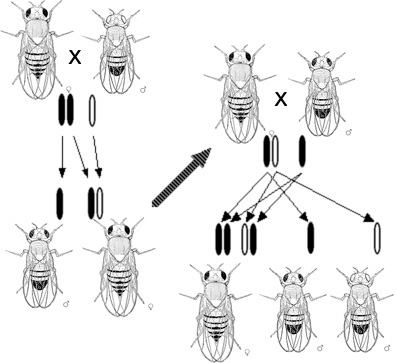
\includegraphics[width=0.7\linewidth]{./figures/genetics/Sexlinked_inheritance_white} 

}

\caption{\href{https://commons.wikimedia.org/wiki/File:Sexlinked_inheritance_white.jpg}{Morgan's observation of sex-linked inheritance of a mutation causing white eyes in Drosophila led him to the hypothesis that genes are located upon chromosomes.}}\label{fig:sexlinked}
\end{figure}

The importance of Mendel's work did not gain wide understanding until 1900, after his death, when Hugo de Vries and other scientists rediscovered his research. William Bateson, a proponent of Mendel's work, coined the word genetics in 1905 (the adjective genetic, derived from the Greek word genesis---γένεσις, ``origin'', predates the noun and was first used in a biological sense in 1860). Bateson both acted as a mentor and was aided significantly by the work of other scientists from Newnham College at Cambridge, specifically the work of Becky Saunders, Nora Darwin Barlow, and Muriel Wheldale Onslow. Bateson popularized the usage of the word genetics to describe the study of inheritance in his inaugural address to the Third International Conference on Plant Hybridization in London in 1906.

After the rediscovery of Mendel's work, scientists tried to determine which molecules in the cell were responsible for inheritance. In 1911, Thomas Hunt Morgan argued that genes are on chromosomes, based on observations of a sex-linked white eye mutation in fruit flies. In 1913, his student Alfred Sturtevant used the phenomenon of genetic linkage to show that genes are arranged linearly on the chromosome.

\hypertarget{molecular-genetics}{%
\section{Molecular genetics}\label{molecular-genetics}}

Although genes were known to exist on chromosomes, chromosomes are composed of both protein and DNA, and scientists did not know which of the two is responsible for inheritance. In 1928, \href{https://en.wikipedia.org/wiki/Frederick_Griffith}{Frederick Griffith} discovered the phenomenon of transformation: dead bacteria could transfer genetic material to ``transform'' other still-living bacteria. Sixteen years later, in 1944, the Avery--MacLeod--McCarty experiment identified DNA as the molecule responsible for transformation. The role of the nucleus as the repository of genetic information in eukaryotes had been established by Hämmerling in 1943 in his work on the single celled alga Acetabularia. The Hershey--Chase experiment in 1952 confirmed that DNA (rather than protein) is the genetic material of the viruses that infect bacteria, providing further evidence that DNA is the molecule responsible for inheritance.

\href{https://en.wikipedia.org/wiki/James_Watson}{James Watson} and \href{https://en.wikipedia.org/wiki/Francis_Crick}{Francis Crick} determined the structure of DNA in 1953, using the X-ray crystallography work of \href{https://en.wikipedia.org/wiki/Rosalind_Franklin}{Rosalind Franklin} and \href{https://en.wikipedia.org/wiki/Maurice_Wilkins}{Maurice Wilkins} that indicated DNA has a helical structure (i.e., shaped like a corkscrew). Their double-helix model had two strands of DNA with the nucleotides pointing inward, each matching a complementary nucleotide on the other strand to form what look like rungs on a twisted ladder. This structure showed that genetic information exists in the sequence of nucleotides on each strand of DNA. The structure also suggested a simple method for replication: if the strands are separated, new partner strands can be reconstructed for each based on the sequence of the old strand. This property is what gives DNA its semi-conservative nature where one strand of new DNA is from an original parent strand.



\begin{figure}

{\centering 
\includegraphics[width=0.7\linewidth]{./figures/genetics/DNA_cartoon} 

}

\caption{A cartoon representation of DNA based on atomic coordinates of \href{https://www.rcsb.org/structure/1bna}{PDB 1BNA}, rendered with open source molecular visualization tool PyMol.}\label{fig:dnacartoon}
\end{figure}

Although the structure of DNA showed how inheritance works, it was still not known how DNA influences the behavior of cells. In the following years, scientists tried to understand how DNA controls the process of protein production. It was discovered that the cell uses DNA as a template to create matching messenger RNA, molecules with nucleotides very similar to DNA. The nucleotide sequence of a messenger RNA is used as a template by ribosomes to create an amino acid sequence in protein; this correspondence between nucleotide sequences and amino acid sequences is known as the genetic code.

With the newfound molecular understanding of inheritance came an explosion of research. One important development was chain-termination DNA sequencing in 1977 by \href{https://en.wikipedia.org/wiki/Frederick_Sanger}{Frederick Sanger}. This technology allows scientists to read the nucleotide sequence of a DNA molecule. In 1983, \href{https://en.wikipedia.org/wiki/Kary_Mullis}{Kary Banks Mullis} developed the polymerase chain reaction, providing a quick way to isolate and amplify a specific section of DNA from a mixture. The efforts of the Human Genome Project, Department of Energy, NIH, and parallel private efforts by Celera Genomics led to the sequencing of the human genome in 2003.

\hypertarget{discrete-inheritance-and-mendels-laws}{%
\section{Discrete inheritance and Mendel's laws}\label{discrete-inheritance-and-mendels-laws}}

At its most fundamental level, inheritance in organisms occurs by passing discrete heritable units, called genes, from parents to offspring. This property was first observed by Gregor Mendel, who studied the segregation of heritable traits in pea plants. In his experiments studying the trait for flower color, Mendel observed that the flowers of each pea plant were either purple or white---but never an intermediate between the two colors. These different, discrete versions of the same gene are called alleles.

In the case of the pea, which is a diploid species, each individual plant has two copies of each gene, one copy inherited from each parent. Many species, including humans, have this pattern of inheritance. Diploid organisms with two copies of the same allele of a given gene are called homozygous at that gene locus, while organisms with two different alleles of a given gene are called heterozygous.

The set of alleles for a given organism is called its genotype, while the observable traits of the organism are called its phenotype. When organisms are heterozygous at a gene, often one allele is called dominant as its qualities dominate the phenotype of the organism, while the other allele is called recessive as its qualities recede and are not observed. Some alleles do not have complete dominance and instead have incomplete dominance by expressing an intermediate phenotype, or codominance by expressing both alleles at once.

When a pair of organisms reproduce sexually, their offspring randomly inherit one of the two alleles from each parent. These observations of discrete inheritance and the segregation of alleles are collectively known as Mendel's first law or the Law of Segregation.

\hypertarget{notation-and-diagrams}{%
\section{Notation and diagrams}\label{notation-and-diagrams}}

Geneticists use diagrams and symbols to describe inheritance. A gene is represented by one or a few letters. Often a ``+'' symbol is used to mark the usual, non-mutant allele for a gene.

In fertilization and breeding experiments (and especially when discussing Mendel's laws) the parents are referred to as the ``P'' generation and the offspring as the ``F1'' (first filial) generation. When the F1 offspring mate with each other, the offspring are called the ``F2'' (second filial) generation. One of the common diagrams used to predict the result of cross-breeding is the Punnett square.

When studying human genetic diseases, geneticists often use pedigree charts to represent the inheritance of traits. These charts map the inheritance of a trait in a family tree.

\hypertarget{multiple-gene-interactions}{%
\section{Multiple gene interactions}\label{multiple-gene-interactions}}

Organisms have thousands of genes, and in sexually reproducing organisms these genes generally assort independently of each other. This means that the inheritance of an allele for yellow or green pea color is unrelated to the inheritance of alleles for white or purple flowers. This phenomenon, known as ``Mendel's second law'' or the ``law of independent assortment,'' means that the alleles of different genes get shuffled between parents to form offspring with many different combinations. (Some genes do not assort independently, demonstrating genetic linkage.

Often different genes can interact in a way that influences the ame trait. In the Blue-eyed Mary (\emph{Omphalodes verna}), for example, there exists a gene with alleles that determine the color of flowers: blue or magenta. Another gene, however, controls whether the flowers have color at all or are white. When a plant has two copies of this white allele, its flowers are white---regardless of whether the first gene has blue or magenta alleles. This interaction between genes is called epistasis, with the second gene epistatic to the first.

Many traits are not discrete features (e.g.~purple or white flowers) but are instead continuous features (e.g.~human height and skin color). These complex traits are products of many genes. The influence of these genes is mediated, to varying degrees, by the environment an organism has experienced. The degree to which an organism's genes contribute to a complex trait is called heritability. Measurement of the heritability of a trait is relative---in a more variable environment, the environment has a bigger influence on the total variation of the trait. For example, human height is a trait with complex causes. It has a heritability of 89\% in the United States. In Nigeria, however, where people experience a more variable access to good nutrition and health care, height has a heritability of only 62\%.

\hypertarget{molecular-basis-for-inheritance}{%
\section{Molecular basis for inheritance}\label{molecular-basis-for-inheritance}}

\hypertarget{dna-and-chromosomes}{%
\subsection{DNA and chromosomes}\label{dna-and-chromosomes}}

The molecular basis for genes is deoxyribonucleic acid (DNA). DNA is composed of a chain of nucleotides, of which there are four types: adenine (A), cytosine (C), guanine (G), and thymine (T). Genetic information exists in the sequence of these nucleotides, and genes exist as stretches of sequence along the DNA chain. Viruses are the only exception to this rule---sometimes viruses use the very similar molecule RNA instead of DNA as their genetic material. Viruses cannot reproduce without a host and are unaffected by many genetic processes, so tend not to be considered living organisms.

DNA normally exists as a double-stranded molecule, coiled into the shape of a double helix. Each nucleotide in DNA preferentially pairs with its partner nucleotide on the opposite strand: A pairs with T, and C pairs with G. Thus, in its two-stranded form, each strand effectively contains all necessary information, redundant with its partner strand. This structure of DNA is the physical basis for inheritance: DNA replication duplicates the genetic information by splitting the strands and using each strand as a template for synthesis of a new partner strand.



\begin{figure}

{\centering 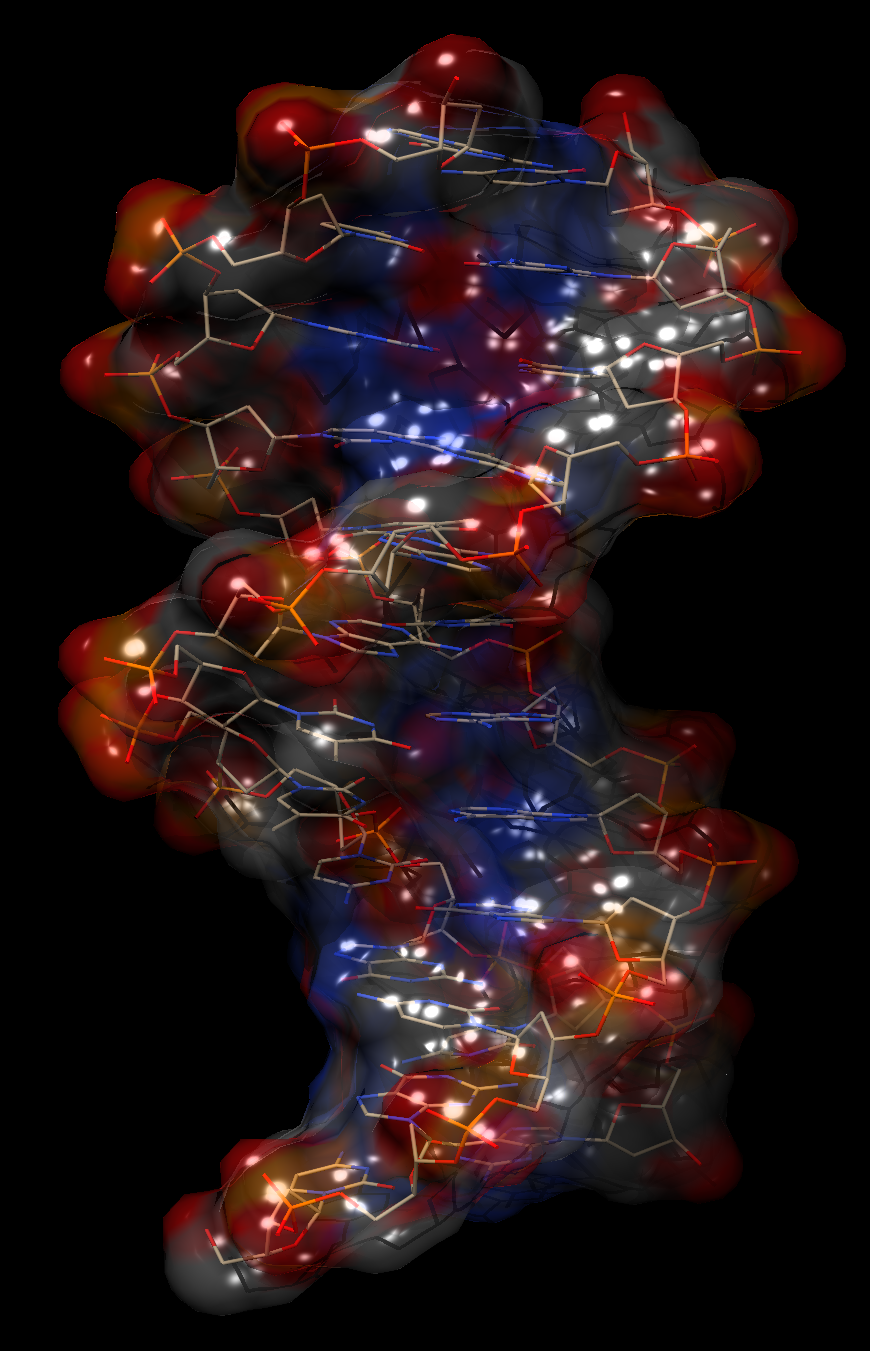
\includegraphics[width=0.7\linewidth]{./figures/dna/dna_surface_transparent} 

}

\caption{The structure of the DNA double helix. A section of DNA. The bases lie horizontally between the two spiraling strands (based on atomic coordinates of \href{https://www.rcsb.org/structure/1bna}{PDB 1bna} rendered with \href{https://www.cgl.ucsf.edu/chimera/}{UCSF Chimera}.)}\label{fig:dnastruc}
\end{figure}

Genes are arranged linearly along long chains of DNA base-pair sequences. In bacteria, each cell usually contains a single circular genophore, while eukaryotic organisms (such as plants and animals) have their DNA arranged in multiple linear chromosomes. These DNA strands are often extremely long; the largest human chromosome, for example, is about 247 million base pairs in length. The DNA of a chromosome is associated with structural proteins that organize, compact, and control access to the DNA, forming a material called chromatin; in eukaryotes, chromatin is usually composed of nucleosomes, segments of DNA wound around cores of histone proteins. The full set of hereditary material in an organism (usually the combined DNA sequences of all chromosomes) is called the genome.

While haploid organisms have only one copy of each chromosome, most animals and many plants are diploid, containing two of each chromosome and thus two copies of every gene. The two alleles for a gene are located on identical loci of the two homologous chromosomes, each allele inherited from a different parent.



\begin{figure}

{\centering 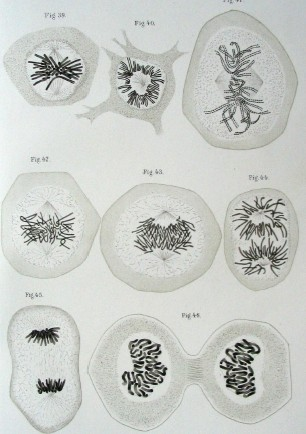
\includegraphics[width=0.7\linewidth]{./figures/genetics/Zellsubstanz-Kern-Kerntheilung} 

}

\caption{\href{https://commons.wikimedia.org/wiki/File:Zellsubstanz-Kern-Kerntheilung.jpg}{Walther Flemming's 1882 diagram of eukaryotic cell division. Chromosomes are copied, condensed, and organized. Then, as the cell divides, chromosome copies separate into the daughter cells.}}\label{fig:celldivision}
\end{figure}

Many species have so-called sex chromosomes that determine the gender of each organism. In humans and many other animals, the Y chromosome contains the gene that triggers the development of the specifically male characteristics. In evolution, this chromosome has lost most of its content and also most of its genes, while the X chromosome is similar to the other chromosomes and contains many genes. The X and Y chromosomes form a strongly heterogeneous pair.

\hypertarget{reproduction}{%
\subsection{Reproduction}\label{reproduction}}

When cells divide, their full genome is copied and each daughter cell inherits one copy. This process, called mitosis, is the simplest form of reproduction and is the basis for asexual reproduction. Asexual reproduction can also occur in multicellular organisms, producing offspring that inherit their genome from a single parent. Offspring that are genetically identical to their parents are called clones.

Eukaryotic organisms often use sexual reproduction to generate offspring that contain a mixture of genetic material inherited from two different parents. The process of sexual reproduction alternates between forms that contain single copies of the genome (haploid) and double copies (diploid). Haploid cells fuse and combine genetic material to create a diploid cell with paired chromosomes. Diploid organisms form haploids by dividing, without replicating their DNA, to create daughter cells that randomly inherit one of each pair of chromosomes. Most animals and many plants are diploid for most of their lifespan, with the haploid form reduced to single cell gametes such as sperm or eggs.

Although they do not use the haploid/diploid method of sexual reproduction, bacteria have many methods of acquiring new genetic information. Some bacteria can undergo conjugation, transferring a small circular piece of DNA to another bacterium. Bacteria can also take up raw DNA fragments found in the environment and integrate them into their genomes, a phenomenon known as transformation. These processes result in horizontal gene transfer, transmitting fragments of genetic information between organisms that would be otherwise unrelated.

\hypertarget{recombination-and-genetic-linkage}{%
\subsection{Recombination and genetic linkage}\label{recombination-and-genetic-linkage}}

The diploid nature of chromosomes allows for genes on different chromosomes to assort independently or be separated from their homologous pair during sexual reproduction wherein haploid gametes are formed. In this way new combinations of genes can occur in the offspring of a mating pair. Genes on the same chromosome would theoretically never recombine. However, they do, via the cellular process of chromosomal crossover. During crossover, chromosomes exchange stretches of DNA, effectively shuffling the gene alleles between the chromosomes. This process of chromosomal crossover generally occurs during meiosis, a series of cell divisions that creates haploid cells.



\begin{figure}

{\centering 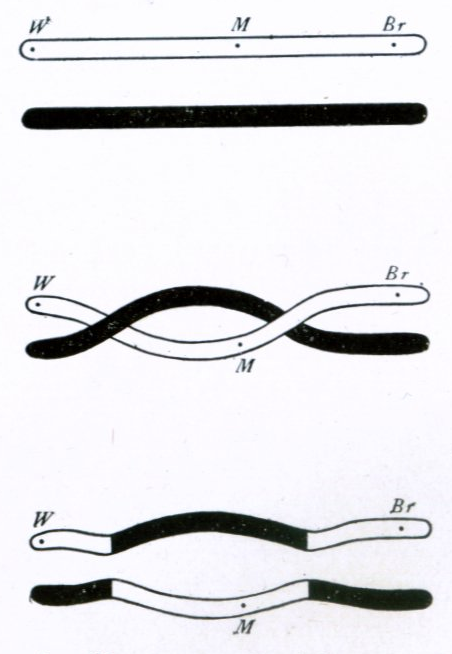
\includegraphics[width=0.7\linewidth]{./figures/genetics/Morgan_crossover_2_cropped} 

}

\caption{\href{https://commons.wikimedia.org/wiki/File:Morgan_crossover_2_cropped.png}{Thomas Hunt Morgan's 1916 illustration of a double crossover between chromosomes.}}\label{fig:crossingover}
\end{figure}

The first cytological demonstration of crossing over was performed by Harriet Creighton and Barbara McClintock in 1931. Their research and experiments on corn provided cytological evidence for the genetic theory that linked genes on paired chromosomes do in fact exchange places from one homolog to the other.

The probability of chromosomal crossover occurring between two given points on the chromosome is related to the distance between the points. For an arbitrarily long distance, the probability of crossover is high enough that the inheritance of the genes is effectively uncorrelated. For genes that are closer together, however, the lower probability of crossover means that the genes demonstrate genetic linkage; alleles for the two genes tend to be inherited together. The amounts of linkage between a series of genes can be combined to form a linear linkage map that roughly describes the arrangement of the genes along the chromosome.

\hypertarget{gene-expression}{%
\section{Gene expression}\label{gene-expression}}

\hypertarget{genetic-code}{%
\subsection{Genetic code}\label{genetic-code}}

Genes generally express their functional effect through the production of proteins, which are complex molecules responsible for most functions in the cell. Proteins are made up of one or more polypeptide chains, each of which is composed of a sequence of amino acids, and the DNA sequence of a gene encodes the amino acid sequence of the corresponding protein. This process begins with the production of a messenger RNA (mRNA) molecule with a sequence matching the gene's DNA sequence, a process called transcription.

This messenger RNA molecule is then used to produce a corresponding amino acid sequence through a process called translation. Each group of three nucleotides in the sequence, called a codon, corresponds either to one of the twenty possible amino acids in a protein or an instruction to end the amino acid sequence; this correspondence is called the genetic code. The flow of information is unidirectional: information is transferred from nucleotide sequences into the amino acid sequence of proteins, but it never transfers from protein back into the sequence of DNA---a phenomenon Francis Crick called the central dogma of molecular biology.

The specific sequence of amino acids results in a unique three-dimensional structure for that protein, and the three-dimensional structures of proteins are related to their functions. Some are simple structural molecules, like the fibers formed by the protein collagen. Proteins can bind to other proteins and simple molecules, sometimes acting as enzymes by facilitating chemical reactions within the bound molecules (without changing the structure of the protein itself). Protein structure is dynamic; the protein hemoglobin bends into slightly different forms as it facilitates the capture, transport, and release of oxygen molecules within mammalian blood.

A single nucleotide difference within DNA can cause a change in the amino acid sequence of a protein. Because protein structures are the result of their amino acid sequences, some changes can dramatically change the properties of a protein by destabilizing the structure or changing the surface of the protein in a way that changes its interaction with other proteins and molecules. For example, sickle-cell anemia is a human genetic disease that results from a single base difference within the coding region for the β-globin section of hemoglobin, causing a single amino acid change that changes hemoglobin's physical properties. Sickle-cell versions of hemoglobin stick to themselves, stacking to form fibers that distort the shape of red blood cells carrying the protein. These sickle-shaped cells no longer flow smoothly through blood vessels, having a tendency to clog or degrade, causing the medical problems associated with this disease.

Some DNA sequences are transcribed into RNA but are not translated into protein products---such RNA molecules are called non-coding RNA. In some cases, these products fold into structures which are involved in critical cell functions (e.g.~ribosomal RNA and transfer RNA). RNA can also have regulatory effects through hybridization interactions with other RNA molecules (e.g.~microRNA).

\hypertarget{nature-and-nurture}{%
\section{Nature and nurture}\label{nature-and-nurture}}

Although genes contain all the information an organism uses to function, the environment plays an important role in determining the ultimate phenotypes an organism displays. The phrase ``nature and nurture'' refers to this complementary relationship. The phenotype of an organism depends on the interaction of genes and the environment. An interesting example is the coat coloration of the Siamese cat. In this case, the body temperature of the cat plays the role of the environment. The cat's genes code for dark hair, thus the hair-producing cells in the cat make cellular proteins resulting in dark hair. But these dark hair-producing proteins are sensitive to temperature (i.e.~have a mutation causing temperature-sensitivity) and denature in higher-temperature environments, failing to produce dark-hair pigment in areas where the cat has a higher body temperature. In a low-temperature environment, however, the protein's structure is stable and produces dark-hair pigment normally. The protein remains functional in areas of skin that are colder---such as its legs, ears, tail and face---so the cat has dark hair at its extremities.

Environment plays a major role in effects of the human genetic disease phenylketonuria. The mutation that causes phenylketonuria disrupts the ability of the body to break down the amino acid phenylalanine, causing a toxic build-up of an intermediate molecule that, in turn, causes severe symptoms of progressive intellectual disability and seizures. However, if someone with the phenylketonuria mutation follows a strict diet that avoids this amino acid, they remain normal and healthy.

A common method for determining how genes and environment (``nature and nurture'') contribute to a phenotype involves studying identical and fraternal twins, or other siblings of multiple births. Identical siblings are genetically the same since they come from the same zygote. Meanwhile, fraternal twins are as genetically different from one another as normal siblings. By comparing how often a certain disorder occurs in a pair of identical twins to how often it occurs in a pair of fraternal twins, scientists can determine whether that disorder is caused by genetic or postnatal environmental factors. However, such tests cannot separate genetic factors from environmental factors affecting fetal development.

\hypertarget{gene-regulation}{%
\section{Gene regulation}\label{gene-regulation}}

The genome of a given organism contains thousands of genes, but not all these genes need to be active at any given moment. A gene is expressed when it is being transcribed into mRNA and there exist many cellular methods of controlling the expression of genes such that proteins are produced only when needed by the cell. Transcription factors are regulatory proteins that bind to DNA, either promoting or inhibiting the transcription of a gene. Within the genome of \emph{Escherichia coli} bacteria, for example, there exists a series of genes necessary for the synthesis of the amino acid tryptophan. However, when tryptophan is already available to the cell, these genes for tryptophan synthesis are no longer needed. The presence of tryptophan directly affects the activity of the genes---tryptophan molecules bind to the tryptophan repressor (a transcription factor), changing the repressor's structure such that the repressor binds to the genes. The tryptophan repressor blocks the transcription and expression of the genes, thereby creating negative feedback regulation of the tryptophan synthesis process.



\begin{figure}

{\centering 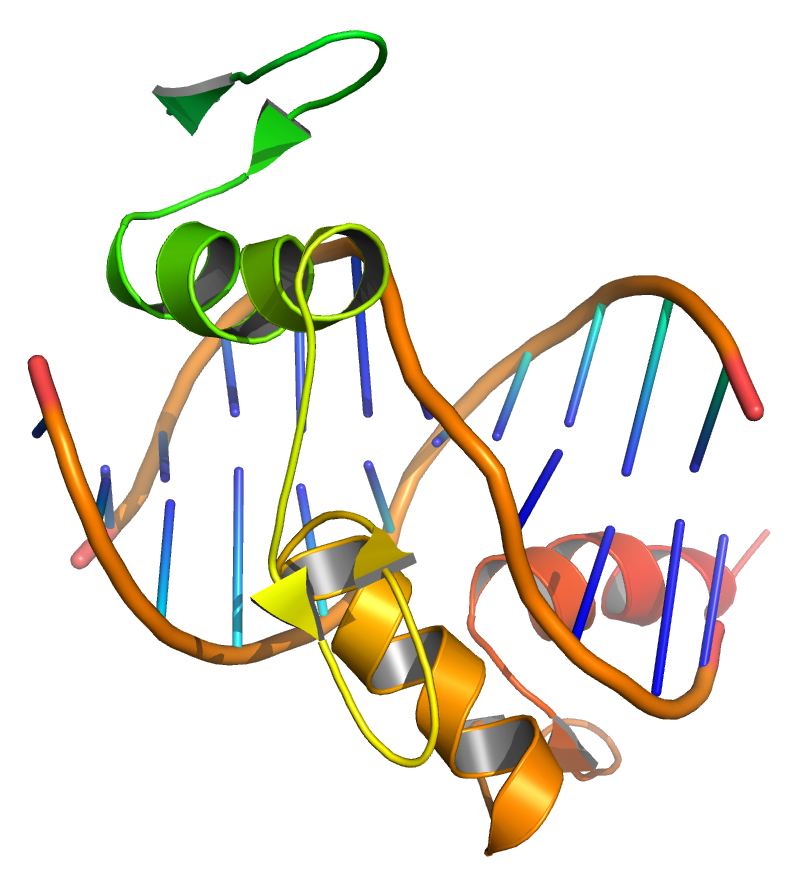
\includegraphics[width=0.7\linewidth]{./figures/genetics/Transcription_factor_DNA_1A1L} 

}

\caption{Transcription factors bind to DNA, influencing the transcription of associated genes. Based on atomic coordinates of \href{https://www.rcsb.org/structure/1a1l}{PDB 1A1L}, rendered with open source molecular visualization tool PyMol.}\label{fig:transcriptionfactor}
\end{figure}

Differences in gene expression are especially clear within multicellular organisms, where cells all contain the same genome but have very different structures and behaviors due to the expression of different sets of genes. All the cells in a multicellular organism derive from a single cell, differentiating into variant cell types in response to external and intercellular signals and gradually establishing different patterns of gene expression to create different behaviors. As no single gene is responsible for the development of structures within multicellular organisms, these patterns arise from the complex interactions between many cells.

Within eukaryotes, there exist structural features of chromatin that influence the transcription of genes, often in the form of modifications to DNA and chromatin that are stably inherited by daughter cells. These features are called ``epigenetic'' because they exist ``on top'' of the DNA sequence and retain inheritance from one cell generation to the next. Because of epigenetic features, different cell types grown within the same medium can retain very different properties. Although epigenetic features are generally dynamic over the course of development, some, like the phenomenon of paramutation, have multigenerational inheritance and exist as rare exceptions to the general rule of DNA as the basis for inheritance.

\hypertarget{genetic-change}{%
\section{Genetic change}\label{genetic-change}}

\hypertarget{mutations}{%
\subsection{Mutations}\label{mutations}}

During the process of DNA replication, errors occasionally occur in the polymerization of the second strand. These errors, called mutations, can affect the phenotype of an organism, especially if they occur within the protein coding sequence of a gene. Error rates are usually very low---1 error in every 10--100 million bases---due to the ``proofreading'' ability of DNA polymerases. Processes that increase the rate of changes in DNA are called mutagenic: mutagenic chemicals promote errors in DNA replication, often by interfering with the structure of base-pairing, while UV radiation induces mutations by causing damage to the DNA structure. Chemical damage to DNA occurs naturally as well and cells use DNA repair mechanisms to repair mismatches and breaks. The repair does not, however, always restore the original sequence.

In organisms that use chromosomal crossover to exchange DNA and recombine genes, errors in alignment during meiosis can also cause mutations. Errors in crossover are especially likely when similar sequences cause partner chromosomes to adopt a mistaken alignment; this makes some regions in genomes more prone to mutating in this way. These errors create large structural changes in DNA sequence -- duplications, inversions, deletions of entire regions -- or the accidental exchange of whole parts of sequences between different chromosomes (chromosomal translocation).

\hypertarget{natural-selection-and-evolution}{%
\section{Natural selection and evolution}\label{natural-selection-and-evolution}}

Mutations alter an organism's genotype and occasionally this causes different phenotypes to appear. Most mutations have little effect on an organism's phenotype, health, or reproductive fitness. Mutations that do have an effect are usually detrimental, but occasionally some can be beneficial. Studies in the fly \emph{Drosophila melanogaster} suggest that if a mutation changes a protein produced by a gene, about 70 percent of these mutations will be harmful with the remainder being either neutral or weakly beneficial.

Population genetics studies the distribution of genetic differences within populations and how these distributions change over time. Changes in the frequency of an allele in a population are mainly influenced by natural selection, where a given allele provides a selective or reproductive advantage to the organism, as well as other factors such as mutation, genetic drift, genetic hitchhiking, artificial selection and migration.

Over many generations, the genomes of organisms can change significantly, resulting in evolution. In the process called adaptation, selection for beneficial mutations can cause a species to evolve into forms better able to survive in their environment. New species are formed through the process of speciation, often caused by geographical separations that prevent populations from exchanging genes with each other.

By comparing the homology between different species' genomes, it is possible to calculate the evolutionary distance between them and when they may have diverged. Genetic comparisons are generally considered a more accurate method of characterizing the relatedness between species than the comparison of phenotypic characteristics. The evolutionary distances between species can be used to form evolutionary trees; these trees represent the common descent and divergence of species over time, although they do not show the transfer of genetic material between unrelated species (known as horizontal gene transfer and most common in bacteria).

\hypertarget{model-organisms}{%
\section{Model organisms}\label{model-organisms}}

Although geneticists originally studied inheritance in a wide range of organisms, researchers began to specialize in studying the genetics of a particular subset of organisms. The fact that significant research already existed for a given organism would encourage new researchers to choose it for further study, and so eventually a few model organisms became the basis for most genetics research. Common research topics in model organism genetics include the study of gene regulation and the involvement of genes in development and cancer.

Organisms were chosen, in part, for convenience---short generation times and easy genetic manipulation made some organisms popular genetics research tools. Widely used model organisms include the gut bacterium \emph{Escherichia coli}, the plant \emph{Arabidopsis thaliana}, baker's yeast (\emph{Saccharomyces cerevisiae}), the nematode \emph{Caenorhabditis elegans}, the common fruit fly (\emph{Drosophila melanogaster}), and the common house mouse (\emph{Mus musculus}).

\hypertarget{medical-genetics}{%
\section{Medical Genetics}\label{medical-genetics}}

\href{https://en.wikipedia.org/wiki/Medical_genetics}{Medical genetics} seeks to understand how genetic variation relates to human health and disease. When searching for an unknown gene that may be involved in a disease, researchers commonly use genetic linkage and genetic pedigree charts to find the location on the genome associated with the disease. At the population level, researchers take advantage of \href{https://en.wikipedia.org/wiki/Mendelian_randomization}{Mendelian randomization} to look for locations in the genome that are associated with diseases, a method especially useful for multigenic traits not clearly defined by a single gene. Once a candidate gene is found, further research is often done on the corresponding (or homologous) genes of model organisms. In addition to studying genetic diseases, the increased availability of genotyping methods has led to the field of pharmacogenetics: the study of how genotype can affect drug responses.

Individuals differ in their inherited tendency to develop cancer, and cancer is a genetic disease. The process of cancer development in the body is a combination of events. Mutations occasionally occur within cells in the body as they divide. Although these mutations will not be inherited by any offspring, they can affect the behavior of cells, sometimes causing them to grow and divide more frequently. There are biological mechanisms that attempt to stop this process; signals are given to inappropriately dividing cells that should trigger cell death, but sometimes additional mutations occur that cause cells to ignore these messages. An internal process of natural selection occurs within the body and eventually mutations accumulate within cells to promote their own growth, creating a cancerous tumor that grows and invades various tissues of the body.

Normally, a cell divides only in response to signals called growth factors and stops growing once in contact with surrounding cells and in response to growth-inhibitory signals. It usually then divides a limited number of times and dies, staying within the epithelium where it is unable to migrate to other organs. To become a cancer cell, a cell has to accumulate mutations in a number of genes (three to seven). A cancer cell can divide without growth factor and ignores inhibitory signals. Also, it is immortal and can grow indefinitely, even after it makes contact with neighboring cells. It may escape from the epithelium and ultimately from the primary tumor. Then, the escaped cell can cross the endothelium of a blood vessel and get transported by the bloodstream to colonize a new organ, forming deadly metastasis. Although there are some genetic predispositions in a small fraction of cancers, the major fraction is due to a set of new genetic mutations that originally appear and accumulate in one or a small number of cells that will divide to form the tumor and are not transmitted to the progeny (somatic mutations). The most frequent mutations are a loss of function of p53 protein, a tumor suppressor, or in the p53 pathway, and gain of function mutations in the Ras proteins, or in other oncogenes.

\hypertarget{research-methods}{%
\section{Research methods}\label{research-methods}}

DNA can be manipulated in the laboratory. \href{https://en.wikipedia.org/wiki/Restriction_enzyme}{Restriction enzymes} are commonly used enzymes that cut DNA at specific sequences, producing predictable fragments of DNA. DNA fragments can be visualized through use of \href{https://en.wikipedia.org/wiki/Gel_electrophoresis}{gel electrophoresis}, which separates fragments according to their length.

The use of \href{https://en.wikipedia.org/wiki/Ligation_(molecular_biology)}{ligation enzymes} allows DNA fragments to be connected. By binding (``ligating'') fragments of DNA together from different sources, researchers can create recombinant DNA, the DNA often associated with genetically modified organisms. Recombinant DNA is commonly used in the context of plasmids: short circular DNA molecules with a few genes on them. In the process known as \href{https://en.wikipedia.org/wiki/Molecular_cloning}{molecular cloning}, researchers can amplify the DNA fragments by inserting plasmids into bacteria and then culturing them on plates of agar (to isolate clones of bacteria cells---``cloning'' can also refer to the various means of creating cloned (``clonal'') organisms).

DNA can also be amplified using a procedure called the \href{https://en.wikipedia.org/wiki/Polymerase_chain_reaction}{polymerase chain reaction (PCR)}. By using specific short sequences of DNA, PCR can isolate and exponentially amplify a targeted region of DNA. Because it can amplify from extremely small amounts of DNA, PCR is also often used to detect the presence of specific DNA sequences.

\hypertarget{dna-sequencing-and-genomics}{%
\subsection{DNA sequencing and genomics}\label{dna-sequencing-and-genomics}}

\href{https://en.wikipedia.org/wiki/DNA_sequencing}{DNA sequencing}, one of the most fundamental technologies developed to study genetics, allows researchers to determine the sequence of nucleotides in DNA fragments. The technique of chain-termination sequencing, developed in 1977 by a team led by Frederick Sanger, is still routinely used to sequence DNA fragments. Using this technology, researchers have been able to study the molecular sequences associated with many human diseases.

As sequencing has become less expensive, researchers have sequenced the genomes of many organisms using a process called genome assembly, which utilizes computational tools to stitch together sequences from many different fragments. These technologies were used to sequence the human genome in the \href{https://en.wikipedia.org/wiki/Human_Genome_Project}{Human Genome Project} completed in 2003. New high-throughput sequencing technologies are dramatically lowering the cost of DNA sequencing, with many researchers hoping to bring the cost of resequencing a human genome down to a thousand dollars.

Next-generation sequencing (or high-throughput sequencing) came about due to the ever-increasing demand for low-cost sequencing. These sequencing technologies allow the production of potentially millions of sequences concurrently. The large amount of sequence data available has created the field of genomics, research that uses computational tools to search for and analyze patterns in the full genomes of organisms. Genomics can also be considered a subfield of bioinformatics, which uses computational approaches to analyze large sets of biological data. A common problem to these fields of research is how to manage and share data that deals with human subject and personally identifiable information.

\hypertarget{genetic-counseling}{%
\section{Genetic counseling}\label{genetic-counseling}}

Genetic counseling is the process of advising individuals and families affected by or at risk of genetic disorders to help them understand and adapt to the medical, psychological and familial implications of genetic contributions to disease. The process integrates:

\begin{itemize}
\tightlist
\item
  Interpretation of family and medical histories to assess the chance of disease occurrence or recurrence
\item
  Education about inheritance, testing, management, prevention, resources
\item
  Counseling to promote informed choices and adaptation to the risk or condition.
\end{itemize}

The practice of advising people about inherited traits began around the turn of the 20th century, shortly after William Bateson suggested that the new medical and biological study of heredity be called ``genetics''. Heredity became intertwined with social reforms when the field of modern eugenics took form. Although initially well-intentioned, ultimately the movement had disastrous consequences. Many states in the United States had laws mandating the sterilization of certain individuals, others were not allowed to immigrate and by the 1930s these ideas were accepted by many other countries including in Germany where euthanaia for the ``genetically defective'' was legalized in 1939. This part of the history of genetics is at the heart of the now ``non directive'' approach to genetic counseling.

Sheldon Clark Reed coined the term genetic counseling in 1947 and published the book Counseling in Medical Genetics in 1955. In 1979, the National Society of Genetic Counselors (NSGC) was founded.

A genetic counselor is an expert with a Master of Science degree in genetic counseling. Programs in North America are accredited by the Accreditation Council for Genetic Counseling (ACGC). There are currently 45 accredited programs in the United States, four accredited programs in Canada, and three programs with the intent to become accredited. Students enter the field from a variety of disciplines, including biology/biological sciences and social sciences such as psychology. Graduate school coursework includes topics such as human genetics, embryology, ethics, research, and counseling theory and techniques. Clinical training including upervised rotations in prenatal, pediatric, adult, cancer, and other subspecialty clinics, as well as non-patient facing rotations in laboratories. Research training typically culminates in a capstone or thesis project.

In the United States genetic counselors are certified by the American Board of Genetic Counseling. In Canada, genetic counselors are certified by the Canadian Association of Genetic Counsellors.

Graduates from an American Board of Genetic Counseling (ABGC) accredited program who have met specific criteria are eligible to take the examination which is offered twice per year by the ABGC. Although not every company requires its counselors to possess a certification, the certification shows that the practitioner has met the standards ``necessary to provide competent genetic counseling services''.

\hypertarget{human-genetics}{%
\section{Human genetics}\label{human-genetics}}

\href{https://en.wikipedia.org/wiki/Human_genetics}{Human genetics} is the study of inheritance as it occurs in human beings.

\hypertarget{genetic-differences-and-inheritance-patterns}{%
\subsection{Genetic differences and inheritance patterns}\label{genetic-differences-and-inheritance-patterns}}

Inheritance of traits for humans are based upon Gregor Mendel's model of inheritance.

\hypertarget{autosomal-dominant-inheritance}{%
\subsection{Autosomal dominant inheritance}\label{autosomal-dominant-inheritance}}

For a recessive trait or disease to be displayed two copies of the trait or disorder needs to be presented. The trait or gene will be located on a non-sex chromosome. Because it takes two copies of a trait to display a trait, many people can unknowingly be carriers of a disease. From an evolutionary perspective, a recessive disease or trait can remain hidden for several generations before displaying the phenotype. Examples of autosomal recessive disorders are \href{https://en.wikipedia.org/wiki/Albinism}{albinism}, \href{https://en.wikipedia.org/wiki/Cystic_fibrosis}{cystic fibrosis}.

\hypertarget{x-linked-and-y-linked-inheritance}{%
\subsection{X-linked and Y-linked inheritance}\label{x-linked-and-y-linked-inheritance}}

X-linked genes are found on the sex X chromosome. X-linked genes just like autosomal genes have both dominant and recessive types. Recessive X-linked disorders are rarely seen in females and usually only affect males. This is because males inherit X-linked genes from the maternal side. Fathers only pass on their Y chromosome to their sons, so no X-linked traits will be inherited from father to son. Men cannot be carriers for recessive X linked traits, as they only have one X chromosome, so any X linked trait inherited from the mother will be expressed.

Females express X-linked disorders when they are homozygous for the disorder and become carriers when they are heterozygous. X-linked dominant inheritance will show the same phenotype as a heterozygote and homozygote. Just like X-linked inheritance, there will be a lack of male-to-male inheritance, which makes it distinguishable from autosomal traits. One example of an X-linked trait is \href{https://en.wikipedia.org/wiki/Coffin–Lowry_syndrome}{Coffin--Lowry syndrome}, which is caused by a mutation in ribosomal protein gene. This mutation results in skeletal, craniofacial abnormalities, mental retardation, and short stature.

X chromosomes in females undergo a process known as X inactivation. X inactivation is when one of the two X chromosomes in females is almost completely inactivated. It is important that this process occurs otherwise a woman would produce twice the amount of normal X chromosome proteins. The mechanism for X inactivation will occur during the embryonic stage. For people with disorders like trisomy X, where the genotype has three X chromosomes, X-inactivation will inactivate all X chromosomes until there is only one X chromosome active. Males with Klinefelter syndrome, who have an extra X chromosome, will also undergo X inactivation to have only one completely active X chromosome.

Y-linked inheritance occurs when a gene, trait, or disorder is transferred through the Y chromosome. Since Y chromosomes can only be found in males, Y linked traits are only passed on from father to son. The testis determining factor, which is located on the Y chromosome, determines the maleness of individuals. Besides the maleness inherited in the Y-chromosome there are no other found Y-linked characteristics.

\hypertarget{pedigrees-analysis}{%
\subsection{Pedigrees analysis}\label{pedigrees-analysis}}

A pedigree is a diagram showing the ancestral relationships and transmission of genetic traits (phenotypes) over several generations in a family (Figure \ref{fig:pedigree}).

The word pedigree is a corruption of the Anglo-Norman French pé de grue or ``crane's foot'', either because the typical lines and split lines (each split leading to different offspring of the one parent line) resemble the thin leg and foot of a crane or because such a mark was used to denote succession in pedigree charts.



\begin{figure}

{\centering 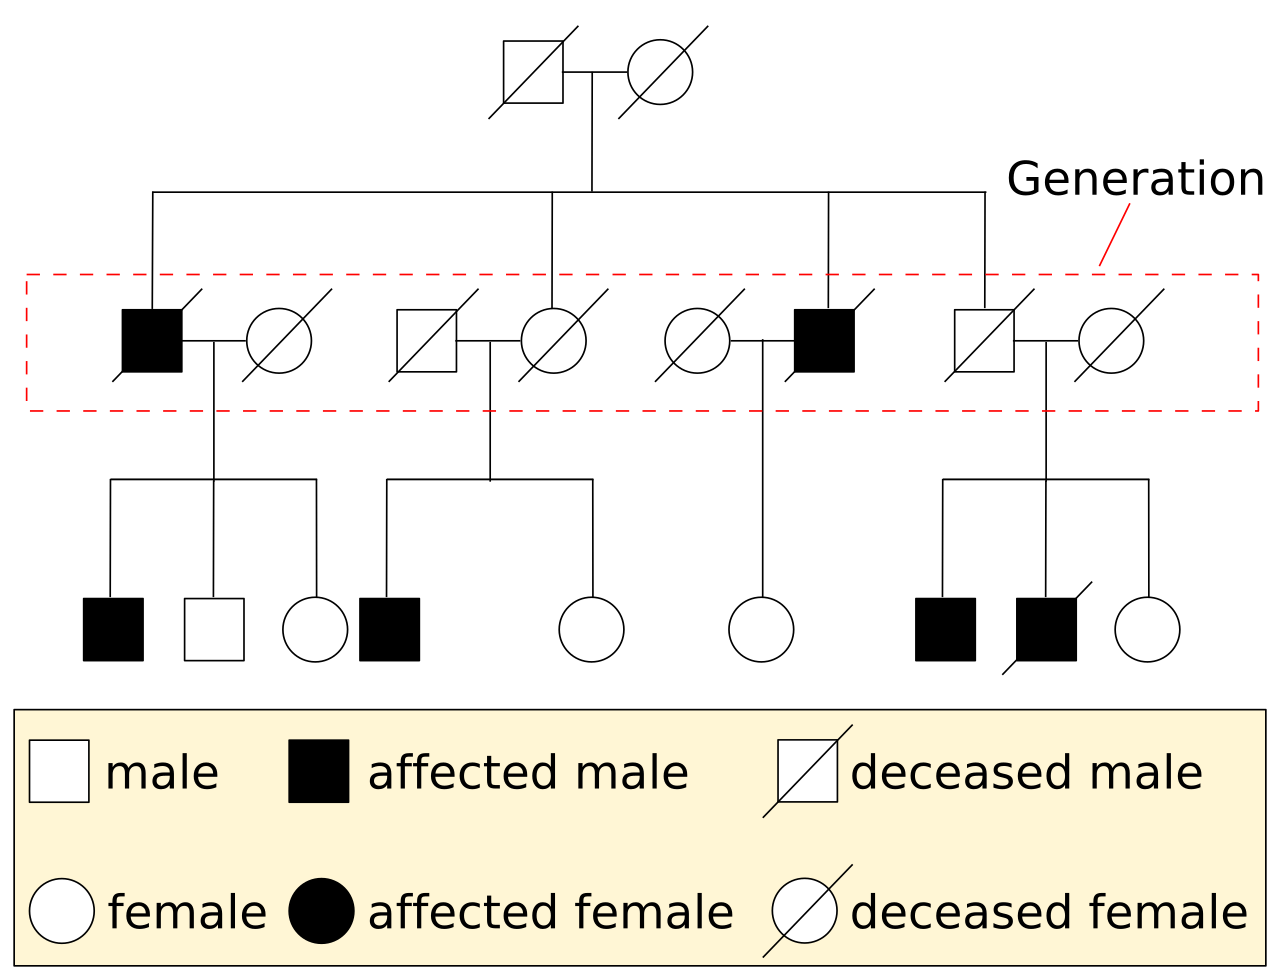
\includegraphics[width=0.7\linewidth]{./figures/genetics/Pedigree-chart-example} 

}

\caption{\href{https://commons.wikimedia.org/wiki/File:Pedigree-chart-example.svg}{A genetic pedigree chart showing three generations.}}\label{fig:pedigree}
\end{figure}

A pedigree results in the presentation of family information in the form of an easily readable chart (Figure \ref{fig:pedigree}. Pedigrees use a standardized set of symbols, squares represent males and circles represent females. Pedigree construction is a family history, and details about an earlier generation may be uncertain as memories fade. If the sex of the person is unknown a diamond is used. Someone with the phenotype in question is represented by a filled-in (darker) symbol. Heterozygotes, when identifiable, are indicated by a shade dot inside a symbol or a half-filled symbol.

Relationships in a pedigree are shown as a series of lines. Parents are connected by a horizontal line and a vertical line leads to their offspring. The offspring are connected by a horizontal sibship line and listed in birth order from left to right. If the offspring are twins then they will be connected by a triangle. If an offspring dies then its symbol will be crossed by a line. If the offspring is still born or aborted it is represented by a small triangle.

Each generation is identified by a Roman numeral (I, II, III, and so on), and each individual within the same generation is identified by an Arabic numeral (1, 2, 3, and so on). Analysis of the pedigree using the principles of Mendelian inheritance can determine whether a trait has a dominant or recessive pattern of inheritance. Pedigrees are often constructed after a family member afflicted with a genetic disorder has been identified. This individual, known as the proband, is indicated on the pedigree by an arrow. These changes may occur yearly or monthly.

Four different traits can be identified by pedigree chart analysis: autosomal dominant, autosomal recessive, x-linked, or y-linked. Partial penetrance can be shown and calculated from pedigrees. Penetrance is the percentage expressed frequency with which individuals of a given genotype manifest at least some degree of a specific mutant phenotype associated with a trait.

A pedigree may be used to establish the probability of a child having a particular disorder or condition. It may be used to discover where the genes in question are located (x, y, or autosome chromosome), and to determine whether a trait is dominant or recessive. When a pedigree shows a condition appearing in a 50:50 ratio between men and women it is considered autosomal. When the condition predominantly affects males in the pedigree it is considered x-linked.

Some examples of dominant traits include: male baldness, astigmatism, and dwarfism. Some examples of recessive traits include: small eyes, little body hair, and tall stature.

\hypertarget{karyotype}{%
\subsection{Karyotype}\label{karyotype}}

A karyotype is picture of all the chromosomes in the metaphase stage arranged according to length and centromere position. A karyotype can also be useful in clinical genetics, due to its ability to diagnose genetic disorders. On a normal karyotype, aneuploidy can be detected by clearly being able to observe any missing or extra chromosomes.



\begin{figure}

{\centering 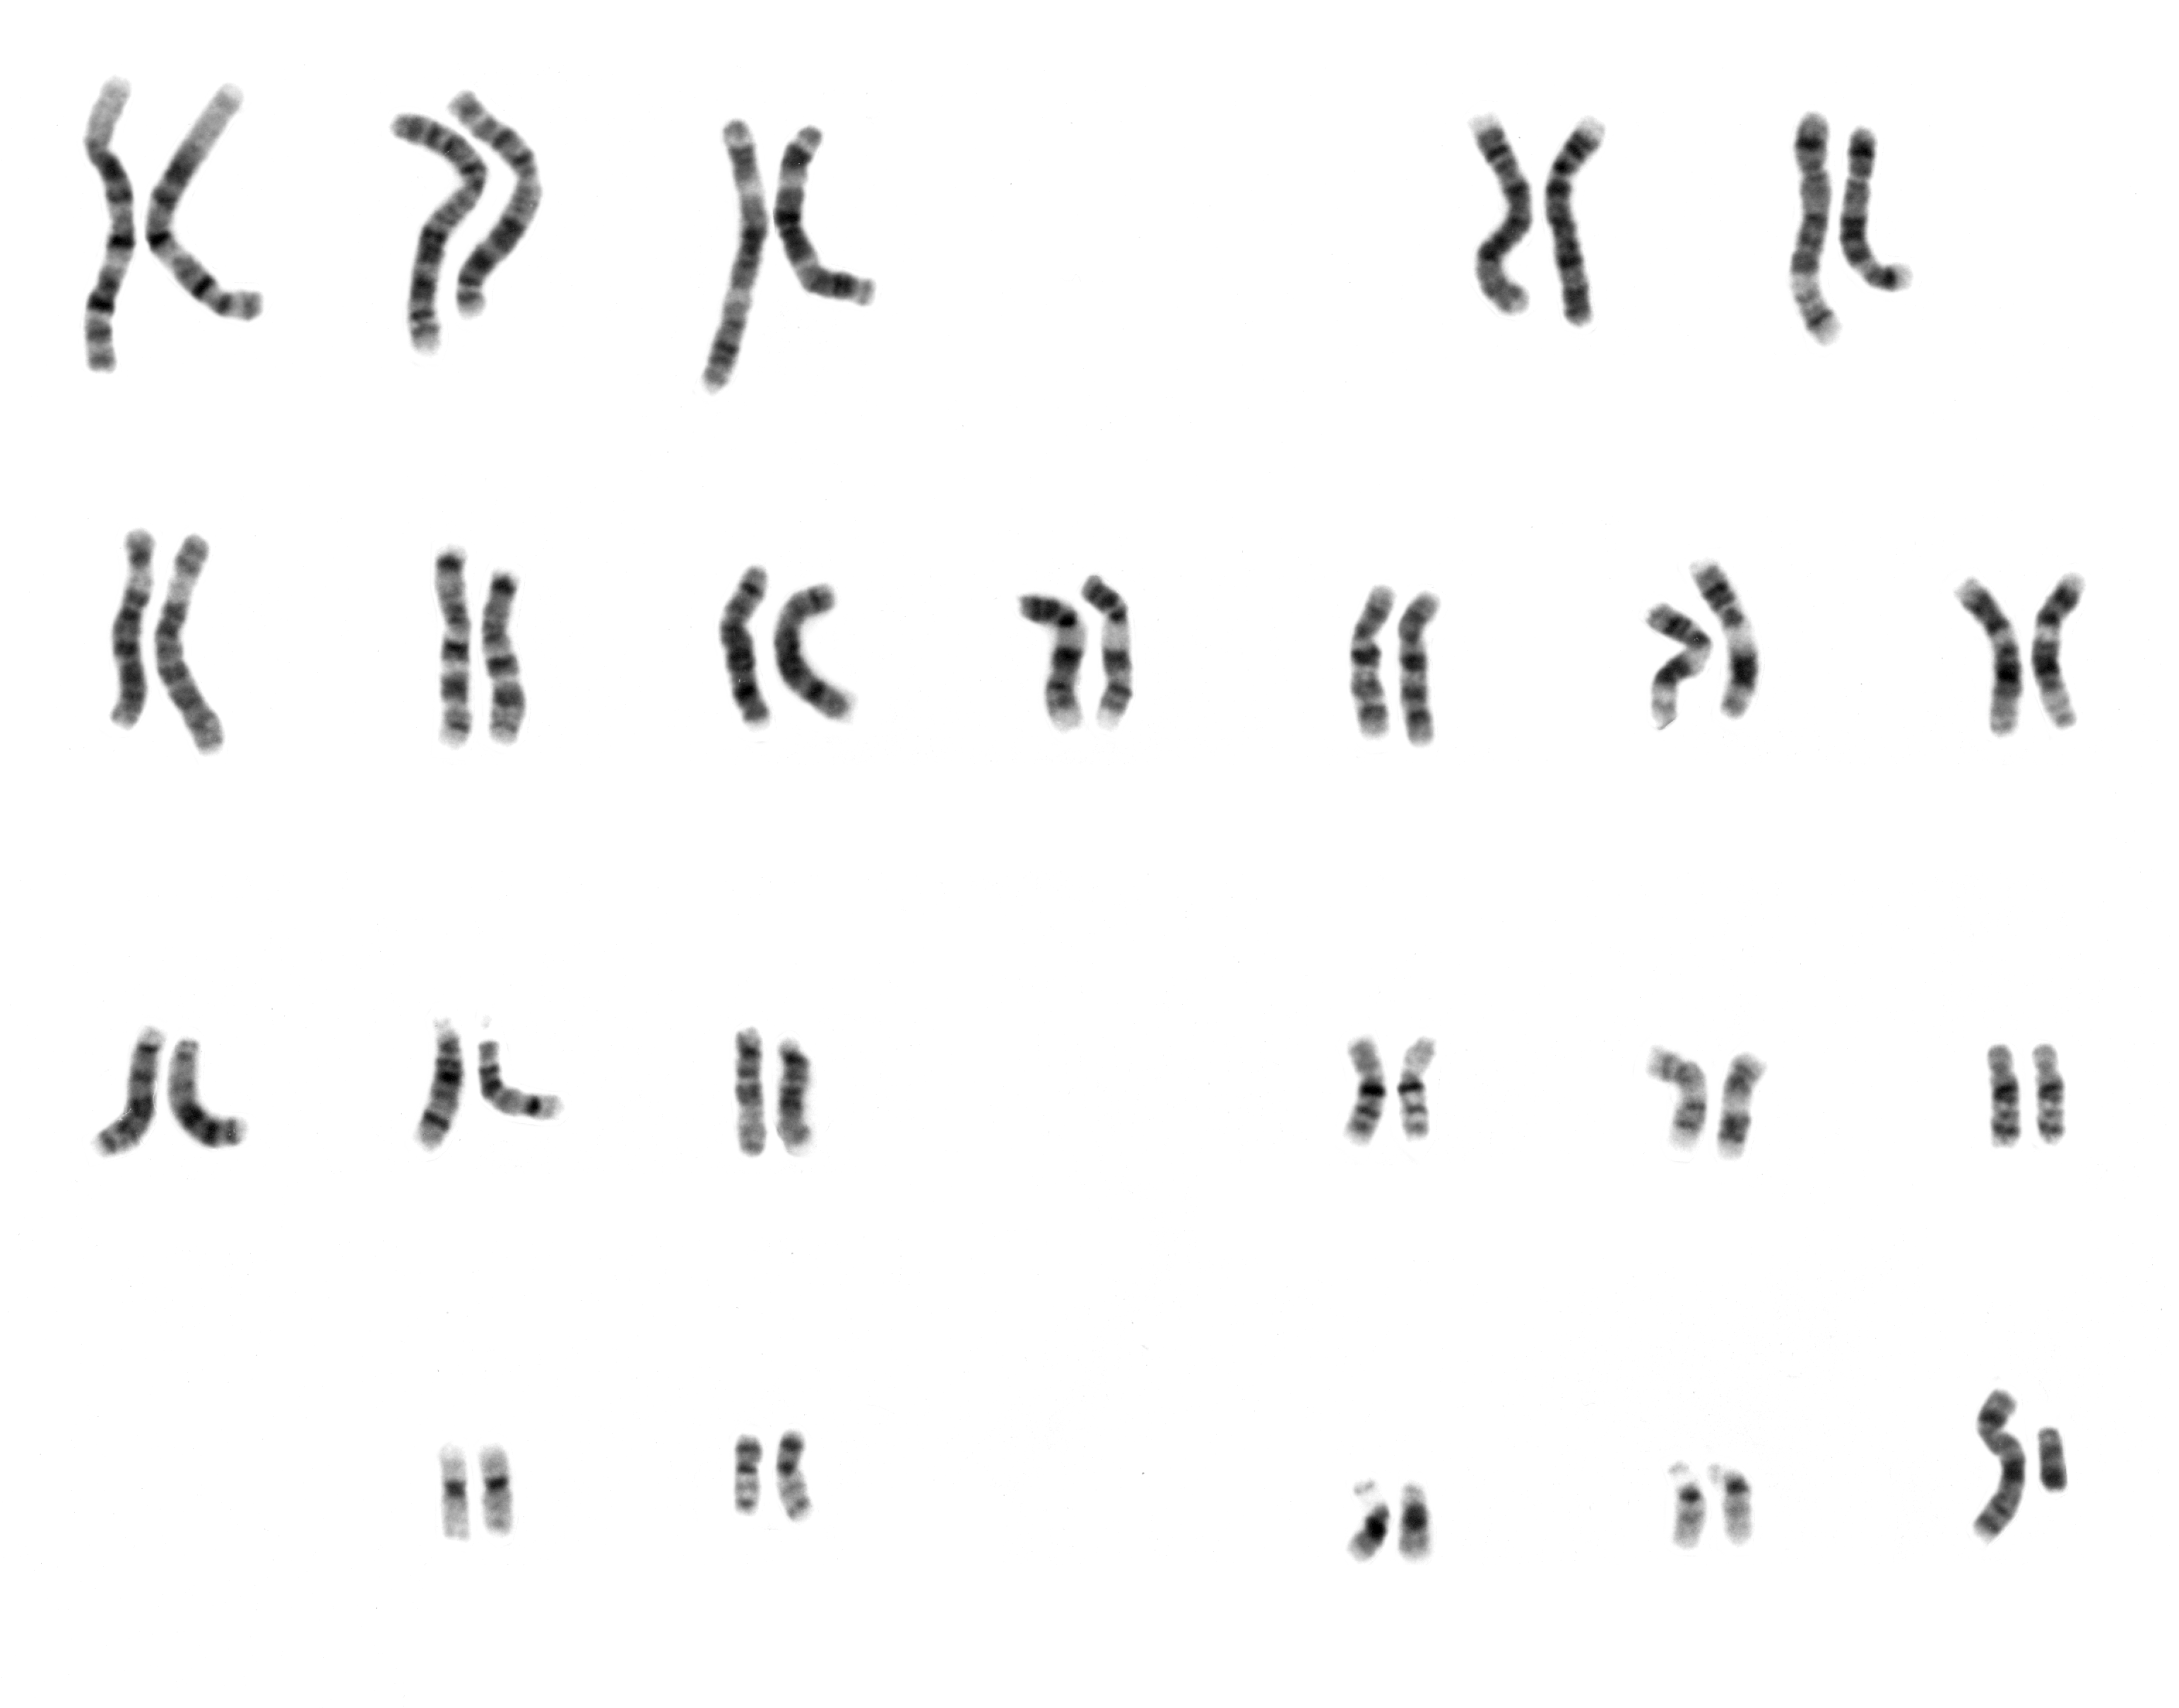
\includegraphics[width=0.7\linewidth]{./figures/chromosomes/human_male_karyotype} 

}

\caption{\href{https://commons.wikimedia.org/wiki/File:NHGRI_human_male_karyotype.png}{Human male karyotype.}}\label{fig:karyotype}
\end{figure}

Giemsa banding, g-banding, of the karyotype can be used to detect deletions, insertions, duplications, inversions, and translocations. G-banding will stain the chromosomes with light and dark bands unique to each chromosome. A FISH, fluorescent in situ hybridization, can be used to observe deletions, insertions, and translocations. FISH uses fluorescent probes to bind to specific sequences of the chromosomes that will cause the chromosomes to fluoresce a unique color.

\hypertarget{genomics}{%
\section{Genomics}\label{genomics}}

Genomics refers to the field of genetics concerned with structural and functional studies of the genome. A genome is all the DNA contained within an organism or a cell including nuclear and mitochondrial DNA. The human genome is the total collection of genes in a human being contained in the human chromosome, composed of over three billion nucleotides.

\hypertarget{population-genetics}{%
\section{Population genetics}\label{population-genetics}}

Population genetics is the branch of evolutionary biology responsible for investigating processes that cause changes in allele and genotype frequencies in populations based upon Mendelian inheritance. Four different forces can influence the frequencies: natural selection, mutation, gene flow (migration), and genetic drift. A population can be defined as a group of interbreeding individuals and their offspring. For human genetics the populations will consist only of the human species. The \href{https://en.wikipedia.org/wiki/Hardy–Weinberg_principle}{Hardy-Weinberg principle} is a widely used principle to determine allelic and genotype frequencies.

In addition to nuclear DNA, humans (like almost all eukaryotes) have mitochondrial DNA. Mitochondria, the ``power houses'' of a cell, have their own DNA. Mitochondria are inherited from one's mother, and their DNA is frequently used to trace maternal lines of descent (see mitochondrial Eve). Mitochondrial DNA is only 16kb in length and encodes for 62 genes.

\hypertarget{eugenics}{%
\section{Eugenics}\label{eugenics}}

\href{https://en.wikipedia.org/wiki/Eugenics}{Eugenics} (from Greek εὐγενής eugenes `well-born' from εὖ eu, `good, well' and γένος genos, `race, stock, kin') is a set of beliefs and practices that aim to improve the genetic quality of a human population by excluding (through a variety of morally criticized means) certain genetic groups judged to be inferior, and promoting other genetic groups judged to be superior. The definition of eugenics has been a matter of debate since the term was coined by \href{https://en.wikipedia.org/wiki/Francis_Galton}{Francis Galton} in 1883. The concept predates the term; Plato suggested applying the principles of selective breeding to humans around 400 BC. Early advocates of eugenics considered it as a way of improving groups of people.

The contemporary history of eugenics began in the early 20th century, when a popular eugenics movement emerged in the United Kingdom, and then spread to many countries, including the United States, Canada, and most European countries. In this period, eugenic ideas were espoused across the political spectrum. Consequently, many countries adopted eugenic policies, intended to improve the quality of their populations' genetic stock. Such programs included both positive measures, such as encouraging individuals deemed particularly ``fit'' to reproduce, and negative measures, such as marriage prohibitions and forced sterilization of people deemed unfit for reproduction. Those deemed ``unfit to reproduce'' often included people with mental or physical disabilities, people who scored in the low ranges on different IQ tests, criminals and ``deviants,'' and members of disfavored minority groups.

The eugenics movement became associated with Nazi Germany and the Holocaust when many of the defendants at the Nuremberg trials attempted to justify their human rights abuses by claiming there was little difference between the Nazi eugenics programs and the U.S. eugenics programs. In the decades following World War II, with more emphasis on human rights, many countries began to abandon eugenics policies, although some Western countries, including the United States, Canada, and Sweden among them, continued to carry out forced sterilizations.

Since the 1980s and 1990s, with new assisted reproductive technology procedures available, such as \href{https://en.wikipedia.org/wiki/Surrogacy}{gestational surrogacy} (available since 1985), \href{https://en.wikipedia.org/wiki/Preimplantation_genetic_diagnosis}{preimplantation genetic diagnosis} (available since 1989), and cytoplasmic transfer (first performed in 1996), concern has grown about the possible revival of a more potent form of eugenics after decades of promoting human rights.

A major criticism of eugenics policies is that, regardless of whether negative or positive policies are used, they are susceptible to abuse because the genetic selection criteria are determined by whichever group has political power at the time. Furthermore, negative eugenics in particular is criticized by many as a violation of basic human rights, which include the right to reproduce. Another criticism is that eugenics policies eventually lead to a loss of genetic diversity, thereby resulting in inbreeding depression due to a loss of genetic variation. Yet another criticism of contemporary eugenics policies is that they propose to permanently and artificially disrupt millions of years of evolution, and that attempting to create genetic lines ``clean'' of ``disorders'' can have far-reaching ancillary downstream effects in the genetic ecology, including negative effects on immunity and species resilience.

The concept of positive eugenics to produce better human beings has existed at least since Plato suggested selective mating to produce a guardian class. In Sparta, every Spartan child was inspected by the council of elders, the Gerousia, which determined if the child was fit to live or not. In the early years of ancient Rome, a Roman father was obliged by law to immediately kill his child if they were physically disabled. Among the ancient Germanic tribes, people who were cowardly, unwarlike or ``stained with abominable vices'' were put to death, usually by being drowned in swamps.

The first formal negative eugenics, that is a legal provision against the birth of allegedly inferior human beings, was promulgated in Western European culture by the Christian Council of Agde in 506, which forbade marriage between cousins.This idea was also promoted by William Goodell (1829--1894) who advocated the castration and spaying of the insane.

The idea of a modern project of improving the human population through a statistical understanding of heredity used to encourage good breeding was originally developed by Francis Galton and, initially, was closely linked to Darwinism and his theory of natural selection. Galton had read his half-cousin Charles Darwin's theory of evolution, which sought to explain the development of plant and animal species, and desired to apply it to humans. Based on his biographical studies, Galton believed that desirable human qualities were hereditary traits, although Darwin strongly disagreed with this elaboration of his theory. In 1883, one year after Darwin's death, Galton gave his research a name: eugenics. With the introduction of genetics, eugenics became associated with genetic determinism, the belief that human character is entirely or in the majority caused by genes, unaffected by education or living conditions. Many of the early geneticists were not Darwinians, and evolution theory was not needed for eugenics policies based on genetic determinism. Throughout its recent history, eugenics has remained controversial.

Eugenics became an academic discipline at many colleges and universities and received funding from many sources. Organizations were formed to win public support and sway opinion towards responsible eugenic values in parenthood, including the British Eugenics Education Society of 1907 and the American Eugenics Society of 1921. Both sought support from leading clergymen and modified their message to meet religious ideals.

Three International Eugenics Conferences presented a global venue for eugenists with meetings in 1912 in London, and in 1921 and 1932 in New York City. Eugenic policies were first implemented in the early 1900s in the United States. It also took root in France, Germany, and Great Britain. Later, in the 1920s and 1930s, the eugenic policy of sterilizing certain mental patients was implemented in other countries including Belgium, Brazil, Canada, Japan and Sweden.

In addition to being practiced in a number of countries, eugenics was internationally organized through the International Federation of Eugenics Organizations. Its scientific aspects were carried on through research bodies such as the Kaiser Wilhelm Institute of Anthropology, Human Heredity, and Eugenics, the Cold Spring Harbour Carnegie Institution for Experimental Evolution, and the Eugenics Record Office. Politically, the movement advocated measures such as sterilization laws. In its moral dimension, eugenics rejected the doctrine that all human beings are born equal and redefined moral worth purely in terms of genetic fitness. Its racist elements included pursuit of a pure ``Nordic race'' or ``Aryan'' genetic pool and the eventual elimination of ``unfit'' races. Many leading British politicians subscribed to the theories of eugenics. Winston Churchill supported the British Eugenics Society and was an honorary vice president for the organization. Churchill believed that eugenics could solve ``race deterioration'' and reduce crime and poverty.

Early critics of the philosophy of eugenics included the American sociologist Lester Frank Ward, the English writer G. K. Chesterton, the German-American anthropologist Franz Boas, who argued that advocates of eugenics greatly over-estimate the influence of biology, and Scottish tuberculosis pioneer and author Halliday Sutherland. Ward's 1913 article ``Eugenics, Euthenics, and Eudemics'', Chesterton's 1917 book Eugenics and Other Evils, and Boas' 1916 article ``Eugenics'' (published in The Scientific Monthly) were all harshly critical of the rapidly growing movement. Sutherland identified eugenists as a major obstacle to the eradication and cure of tuberculosis in his 1917 address ``Consumption: Its Cause and Cure'', and criticism of eugenists and Neo-Malthusians in his 1921 book Birth Control led to a writ for libel from the eugenist Marie Stopes. Several biologists were also antagonistic to the eugenics movement, including Lancelot Hogben. Other biologists such as J. B. S. Haldane and R. A. Fisher expressed skepticism in the belief that sterilization of ``defectives'' would lead to the disappearance of undesirable genetic traits.

Among institutions, the Catholic Church was an opponent of state-enforced sterilizations. Attempts by the Eugenics Education Society to persuade the British government to legalize voluntary sterilization were opposed by Catholics and by the Labour Party. The American Eugenics Society initially gained some Catholic supporters, but Catholic support declined following the 1930 papal encyclical Casti connubii. In this, Pope Pius XI explicitly condemned sterilization laws: ``Public magistrates have no direct power over the bodies of their subjects; therefore, where no crime has taken place and there is no cause present for grave punishment, they can never directly harm, or tamper with the integrity of the body, either for the reasons of eugenics or for any other reason.''

As a social movement, eugenics reached its greatest popularity in the early decades of the 20th century, when it was practiced around the world and promoted by governments, institutions, and influential individuals. Many countries enacted various eugenics policies, including: genetic screenings, birth control, promoting differential birth rates, marriage restrictions, segregation (both racial segregation and sequestering the mentally ill), compulsory sterilization, forced abortions or forced pregnancies, ultimately culminating in genocide. By 2014, gene selection (rather than ``people selection'') was made possible through advances in genome editing, leading to what is sometimes called new eugenics, also known as ``neo-eugenics'', ``consumer eugenics'', or ``liberal eugenics''.

The scientific reputation of eugenics started to decline in the 1930s, a time when Ernst Rüdin used eugenics as a justification for the racial policies of Nazi Germany. Adolf Hitler had praised and incorporated eugenic ideas in Mein Kampf in 1925 and emulated eugenic legislation for the sterilization of ``defectives'' that had been pioneered in the United States once he took power. Some common early 20th century eugenics methods involved identifying and classifying individuals and their families, including the poor, mentally ill, blind, deaf, developmentally disabled, promiscuous women, homosexuals, and racial groups (such as the Roma and Jews in Nazi Germany) as ``degenerate'' or ``unfit'', and therefore led to segregation, institutionalization, sterilization, euthanasia, and even mass murder.

By the end of World War II, many eugenics laws were abandoned, having become associated with Nazi Germany. H. G. Wells, who had called for ``the sterilization of failures'' in 1904, stated in his 1940 book The Rights of Man: Or What are we fighting for? that among the human rights, which he believed should be available to all people, was ``a prohibition on mutilation, sterilization, torture, and any bodily punishment''. After World War II, the practice of ``imposing measures intended to prevent births within {[}a national, ethnical, racial or religious{]} group'' fell within the definition of the new international crime of genocide, set out in the Convention on the Prevention and Punishment of the Crime of Genocide. The Charter of Fundamental Rights of the European Union also proclaims ``the prohibition of eugenic practices, in particular those aiming at selection of persons''. In spite of the decline in discriminatory eugenics laws, some government mandated sterilizations continued into the 21st century. During the ten years President Alberto Fujimori led Peru from 1990 to 2000, 2,000 persons were allegedly involuntarily sterilized. China maintained its one-child policy until 2015 as well as a suite of other eugenics based legislation to reduce population size and manage fertility rates of different populations. In 2007 the United Nations reported coercive sterilizations and hysterectomies in Uzbekistan. During the years 2005 to 2013, nearly one-third of the 144 California prison inmates who were sterilized did not give lawful consent to the operation.

Developments in genetic, genomic, and reproductive technologies at the end of the 20th century have raised numerous questions regarding the ethical status of eugenics, effectively creating a resurgence of interest in the subject.

Prenatal screening can be considered a form of contemporary eugenics because it may lead to abortions of children with undesirable traits.

The first major challenge to conventional eugenics based on genetic inheritance was made in 1915 by Thomas Hunt Morgan. He demonstrated the event of genetic mutation occurring outside of inheritance involving the discovery of the hatching of a fruit fly (Drosophila melanogaster) with white eyes from a family with red eyes, demonstrating that major genetic changes occurred outside of inheritance. Additionally, Morgan criticized the view that certain traits, such as intelligence and criminality, were hereditary because these traits were subjective. Despite Morgan's public rejection of eugenics, much of his genetic research was adopted by proponents of eugenics.

The heterozygote test is used for the early detection of recessive hereditary diseases, allowing for couples to determine if they are at risk of passing genetic defects to a future child. The goal of the test is to estimate the likelihood of passing the hereditary disease to future descendants.

There are examples of eugenic acts that managed to lower the prevalence of recessive diseases, although not influencing the prevalence of heterozygote carriers of those diseases. The elevated prevalence of certain genetically transmitted diseases among the Ashkenazi Jewish population (Tay--Sachs, cystic fibrosis, Canavan's disease, and Gaucher's disease), has been decreased in current populations by the application of genetic screening.



\chapter{Reproduction of Cells and Organisms}\label{reproduction-of-cells-and-organisms}

\hypertarget{the-cell}{%
\section{The Cell}\label{the-cell}}

The \href{https://en.wikipedia.org/wiki/Cell_(biology)}{cell} (from Latin cella, meaning ``small room'') is the basic structural, functional, and biological unit of all known organisms. A cell is the smallest unit of life. Cells are often called the ``building blocks of life''. The study of cells is called cell biology, cellular biology, or cytology.

Cells consist of cytoplasm enclosed within a membrane, which contains many biomolecules such as proteins and nucleic acids. Most plant and animal cells are only visible under a microscope, with dimensions between 1 and 100 micrometres. Organisms can be classified as unicellular (consisting of a single cell such as bacteria) or multicellular (including plants and animals). Most unicellular organisms are classed as microorganisms.

The number of cells in plants and animals varies from species to species, it has been estimated that humans contain somewhere around 40 trillion (4×10\textsuperscript{13}) cells. The human brain accounting for around 80 billion of these cells.

Cells were discovered by Robert Hooke in 1665, who named them for their resemblance to cells inhabited by Christian monks in a monastery. Cell theory, first developed in 1839 by Matthias Jakob Schleiden and Theodor Schwann, states that all organisms are composed of one or more cells, that cells are the fundamental unit of structure and function in all living organisms, and that all cells come from pre-existing cells. Cells emerged on Earth at least 3.5 billion years ago.



\begin{figure}

{\centering 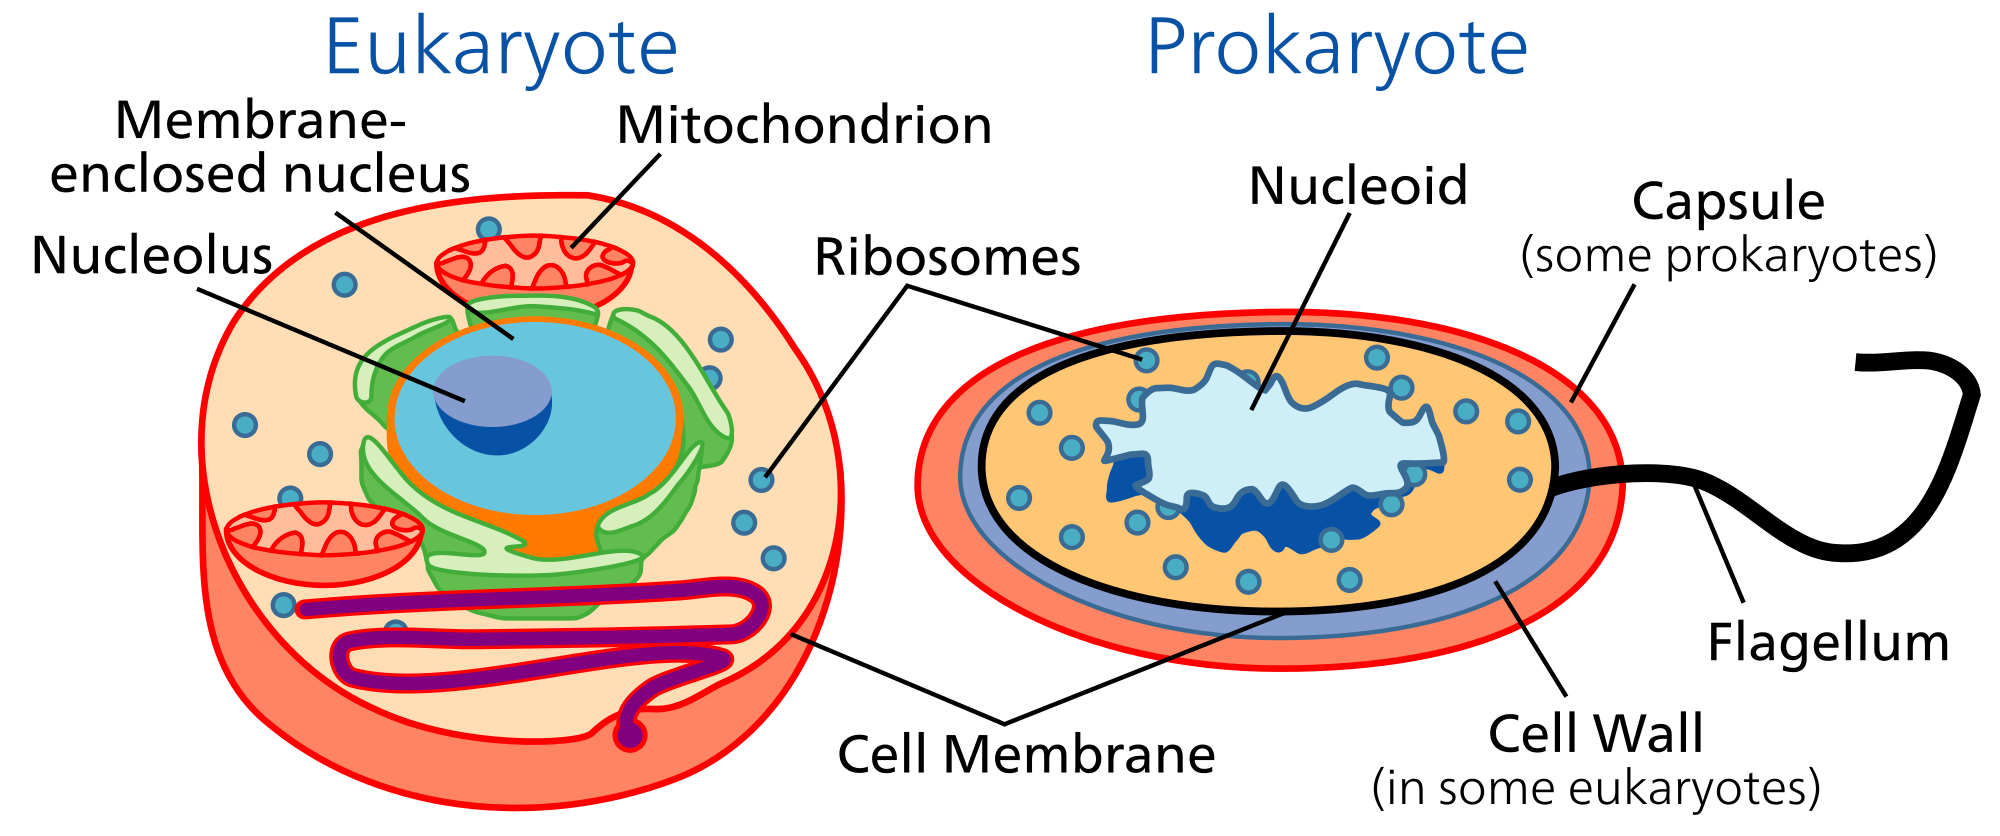
\includegraphics[width=0.7\linewidth]{./figures/reproduction/Celltypes} 

}

\caption{\href{htps://en.wikipedia.org/wiki/Cell_(biology)\#/media/File:Celltypes.svg}{Characteristic features of eukaryotic and prokaryotic cells.}}\label{fig:comparison}
\end{figure}

Cells are of two types: eukaryotic, which contain a nucleus, and prokaryotic, which do not. Prokaryotes are single-celled organisms, while eukaryotes can be either single-celled or multicellular.

\begin{longtable}[t]{>{\raggedright\arraybackslash}p{10em}>{\raggedright\arraybackslash}p{10em}>{\raggedright\arraybackslash}p{10em}}
\caption{\label{tab:eupro}Comparison of the main features of prokaryotic and eukaryotic cells.}\\
\toprule
 & Prokaryotes & Eukaryotes\\
\midrule
\rowcolor{gray!6}  Typical organisms & bacteria, archaea & protists, fungi, plants, animals\\
Typical size & \textasciitilde{}1-5 µm & \textasciitilde{}10-100 µm\\
\rowcolor{gray!6}  Type of nucleus & nucleoid region, true nucleus with double membrane & no true nucleus\\
DNA & circular (usually) & linear molecules (chromosomes) with histone proteins\\
\rowcolor{gray!6}  RNA/protein synthesis & coupled in the cytoplasm & RNA synthesis in the nucleus, protein synthesis in the cytoplasm\\
\addlinespace
Ribosomes & 50S and 30S & 60S and 40S\\
\rowcolor{gray!6}  Cytoplasmic structure & very few structures & highly structured by endomembranes and a cytoskeleton\\
Cell movement & flagella made of flagellin & flagella and cilia containing microtubules, lamellipodia and filopodia containing actin\\
\rowcolor{gray!6}  Mitochondria & none & one to several thousand\\
Chloroplasts & none & in algae and plants\\
\addlinespace
\rowcolor{gray!6}  Organization & usually single cells & single cells, colonies, higher multicellular organisms with specialized cells\\
Cell division & binary fission (simple division) & mitosis (fission or budding), meiosis\\
\rowcolor{gray!6}  Chromosomes & single chromosome & more than one chromosome\\
Membranes & cell membrane & cell membrane and membrane-bound organelles\\
\bottomrule
\end{longtable}

\hypertarget{prokaryotic-cells}{%
\section{Prokaryotic cells}\label{prokaryotic-cells}}

Prokaryotes include \href{https://en.wikipedia.org/wiki/Bacteria}{bacteria} and \href{https://en.wikipedia.org/wiki/Archaea}{archaea}, two of the three domains of life. Prokaryotic cells were the first form of life on Earth, characterized by having vital biological processes including cell signaling. They are simpler and smaller than eukaryotic cells, and lack a nucleus, and other membrane-bound organelles. The DNA of a prokaryotic cell consists of a single circular chromosome that is in direct contact with the cytoplasm. The nucleus-like region in the cytoplasm is called the nucleoid. Most prokaryotes are the smallest of all organisms ranging from 0.5 to 2.0 µm in diameter.

A prokaryotic cell has three regions:

\begin{itemize}
\item
  Enclosing the cell is the cell envelope -- generally consisting of a plasma membrane covered by a cell wall. Gram-positive bacteria possess a thick cell wall containing many layers of peptidoglycan and teichoic acids. In contrast, Gram-negative bacteria have a relatively thin cell wall consisting of a few layers of peptidoglycan surrounded by a second lipid membrane containing lipopolysaccharides and lipoproteins. Some bacteria have cell wall structures that are neither classically Gram-positive or Gram-negative. This includes clinically important bacteria such as Mycobacteria which have a thick peptidoglycan cell wall like a Gram-positive bacterium, but also a second outer layer of lipids. Though most prokaryotes have both a cell membrane and a cell wall, there are exceptions such as Mycoplasma (bacteria) and Thermoplasma (archaea) which only possess the cell membrane layer. In many bacteria, an S-layer of rigidly arrayed protein molecules covers the outside of the cell. This layer provides chemical and physical protection for the cell surface and can act as a macromolecular diffusion barrier. The envelope gives rigidity to the cell and separates the interior of the cell from its environment, serving as a protective filter. The cell wall consists of peptidoglycan in bacteria, and acts as an additional barrier against exterior forces. It also prevents the cell from expanding and bursting (cytolysis) from osmotic pressure due to a hypotonic environment.
\item
  Inside the cell is the cytoplasmic region that contains the genome (DNA), ribosomes and various sorts of inclusions. The genetic material is freely found in the cytoplasm. Prokaryotes can carry extrachromosomal DNA elements called plasmids, which are usually circular. Linear bacterial plasmids have been identified in several species of spirochete bacteria, including members of the genus Borrelia notably Borrelia burgdorferi, which causes Lyme disease. Though not forming a nucleus, the DNA is condensed in a nucleoid. Plasmids encode additional genes, such as antibiotic resistance genes.
\item
  On the outside, flagella and pili project from the cell's surface. These are structures (not present in all prokaryotes) made of proteins that facilitate movement and communication between cells.
\end{itemize}

\hypertarget{eukaryotic-cells}{%
\section{Eukaryotic cells}\label{eukaryotic-cells}}

Plants, animals, fungi, and protists are all eukaryotic. These cells are about fifteen times wider than a typical prokaryote and can be as much as a thousand times greater in volume. The main distinguishing feature of eukaryotes as compared to prokaryotes is compartmentalization: the presence of membrane-bound organelles (compartments) in which specific activities take place. Most important among these is a cell nucleus, an organelle that houses the cell's DNA. This nucleus gives the eukaryote its name, which means ``true kernel (nucleus)''. Other characteristics include:



\begin{figure}

{\centering 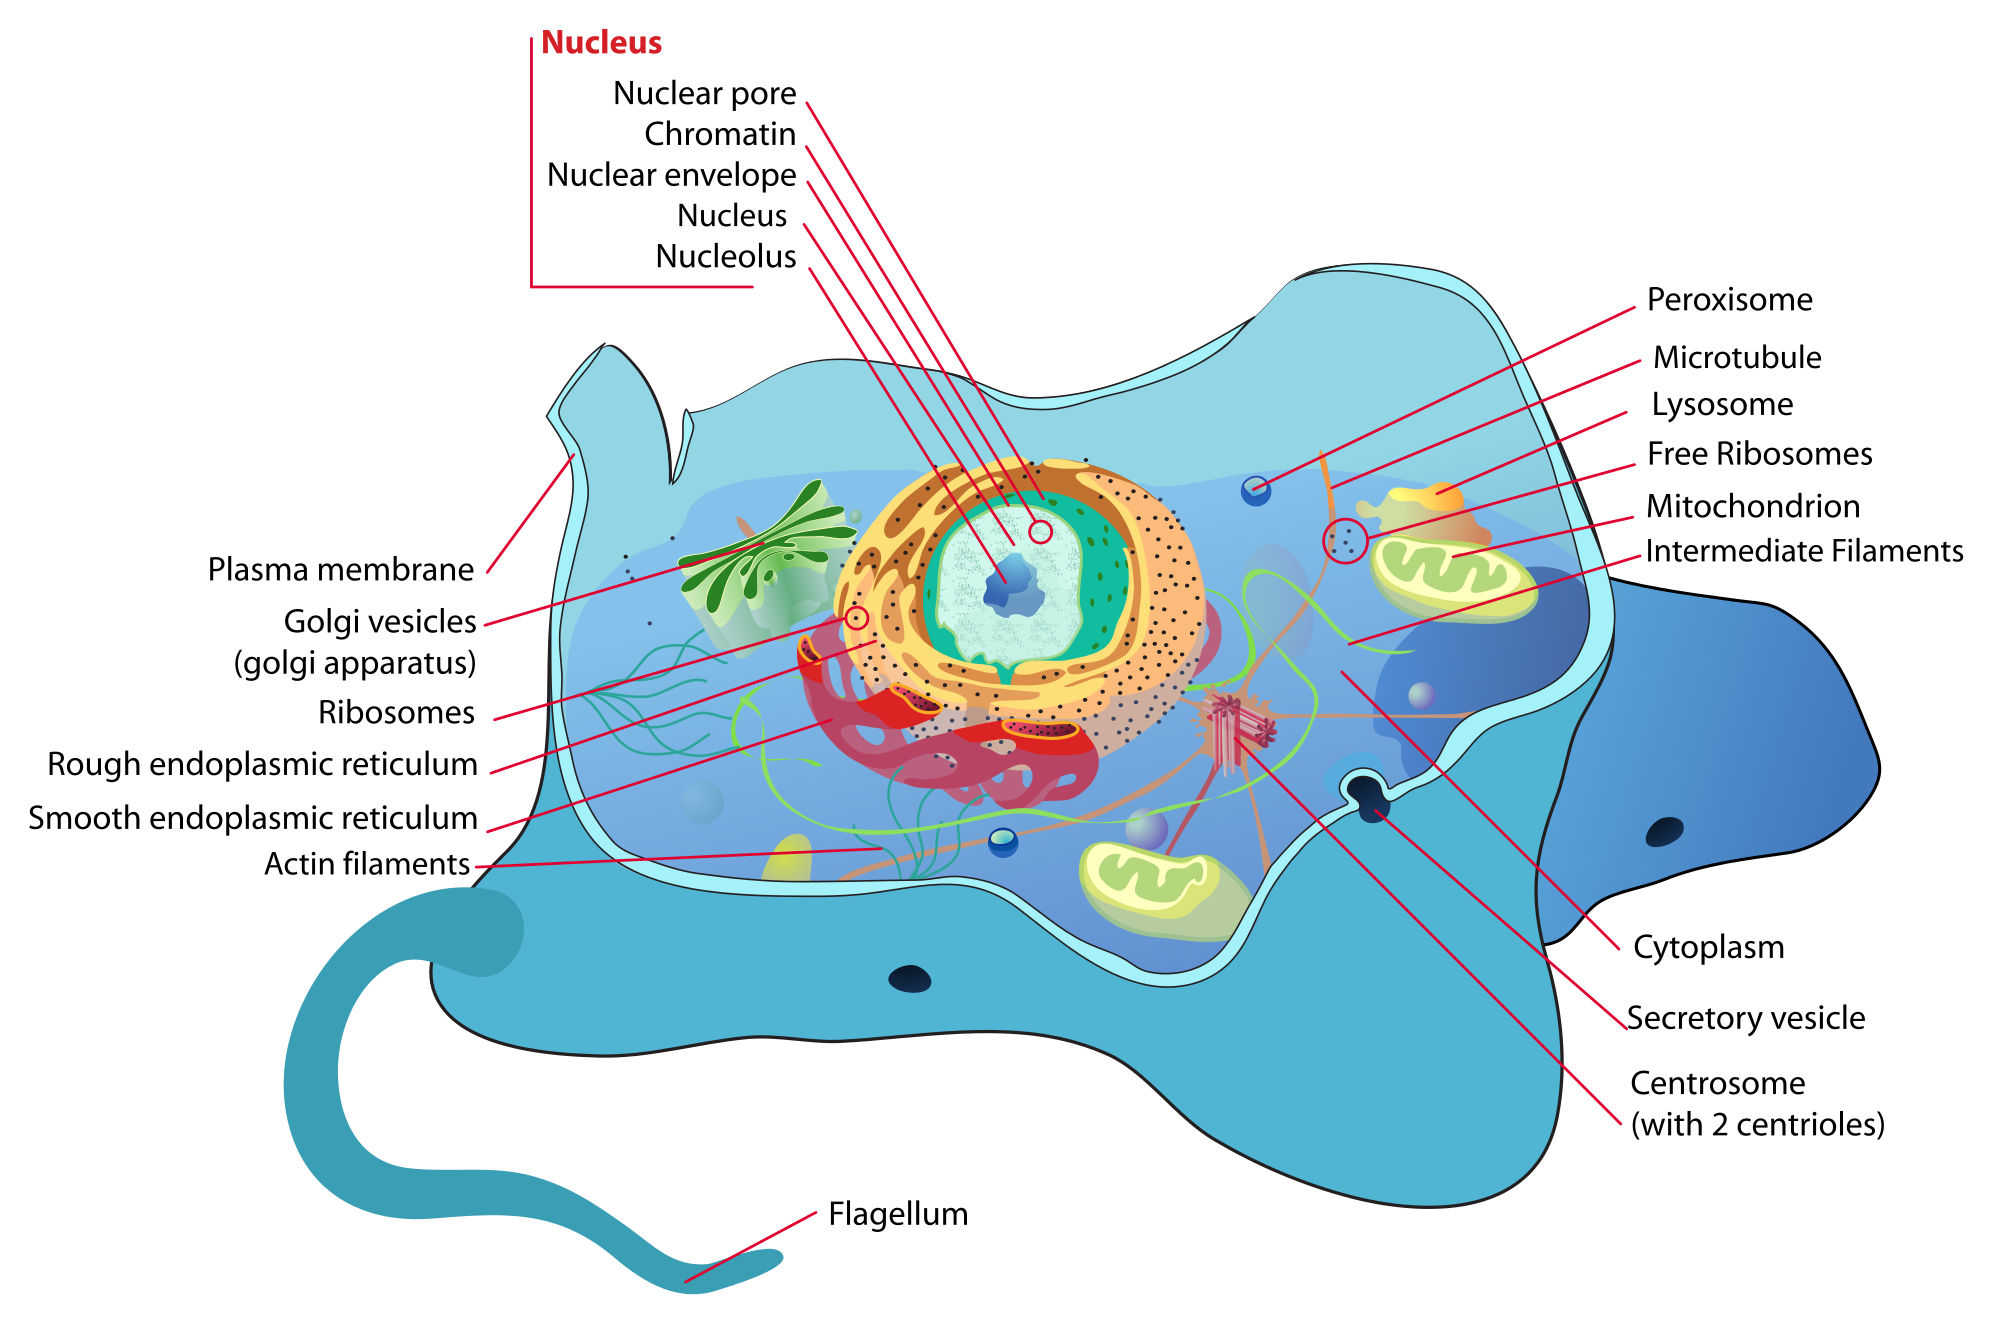
\includegraphics[width=0.7\linewidth]{./figures/reproduction/Animal_cell_structure_en} 

}

\caption{\href{https://commons.wikimedia.org/wiki/File:Animal_cell_structure_en.svg}{Structure of a typical animal cell}}\label{fig:animalcell}
\end{figure}



\begin{figure}

{\centering 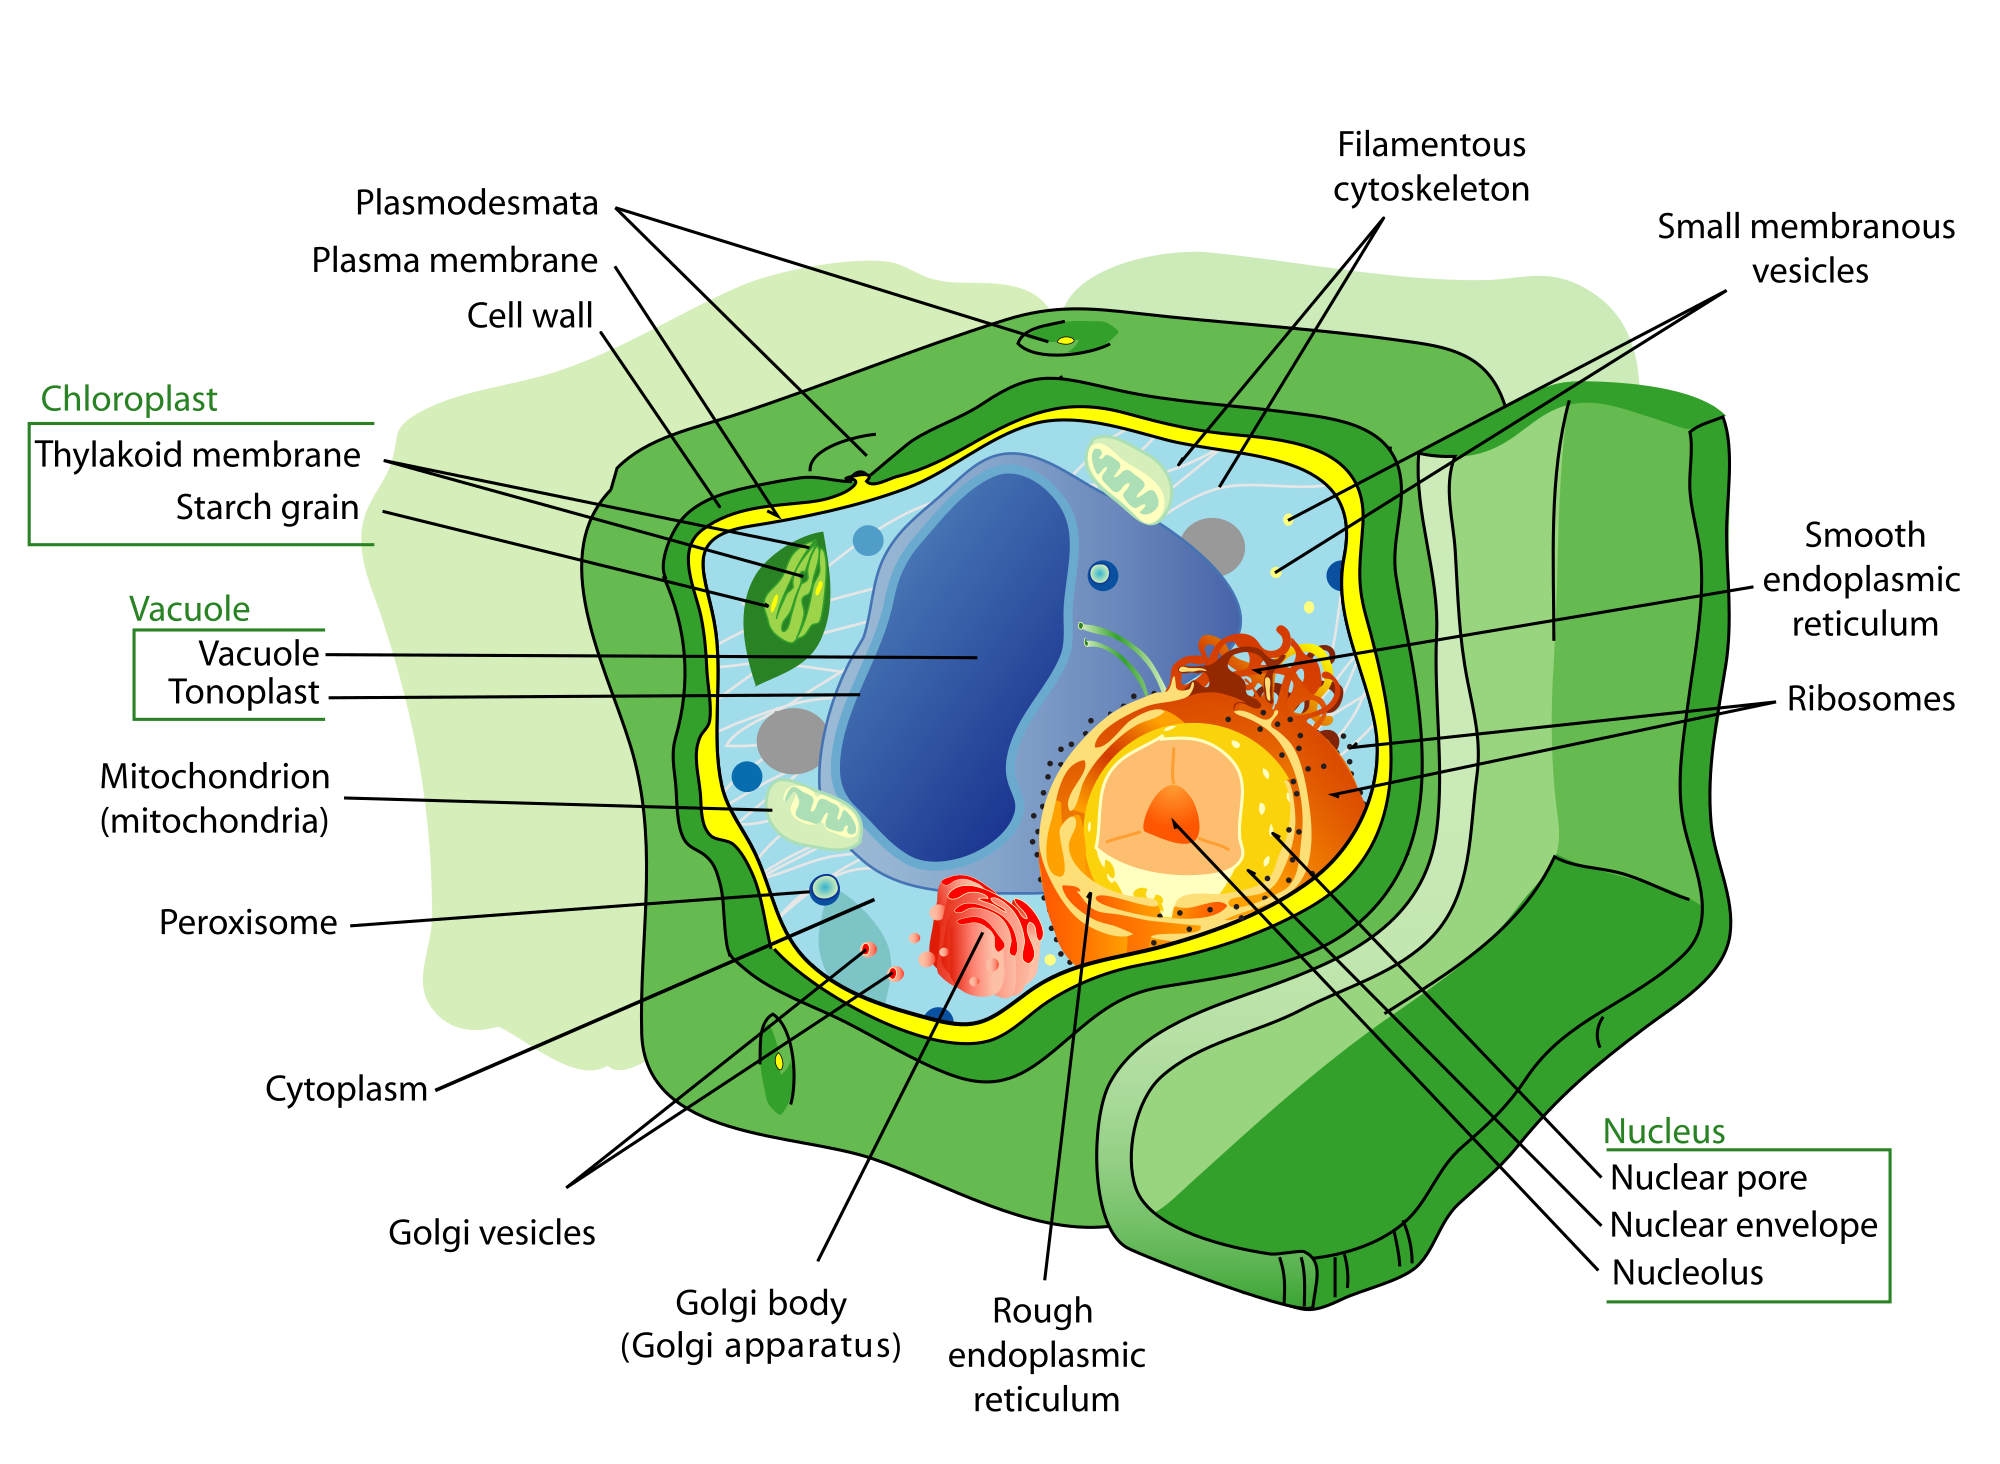
\includegraphics[width=0.7\linewidth]{./figures/reproduction/Plant_cell_structure-en} 

}

\caption{\href{https://commons.wikimedia.org/wiki/File:Plant_cell_structure-en.svg}{Structure of a typical plant cell}}\label{fig:plantcell}
\end{figure}

\begin{itemize}
\tightlist
\item
  The plasma membrane resembles that of prokaryotes in function, with minor differences in the setup. Cell walls may or may not be present.
\item
  The eukaryotic DNA is organized in one or more linear molecules, called chromosomes, which are associated with histone proteins. All chromosomal DNA is stored in the cell nucleus, separated from the cytoplasm by a membrane. Some eukaryotic organelles such as mitochondria also contain some DNA.
\item
  Many eukaryotic cells are ciliated. Cilia play important roles in chemosensation, mechanosensation, and thermosensation. Each cilium may thus be ``viewed as a sensory cellular antennae that coordinates a large number of cellular signaling pathways, sometimes coupling the signaling to ciliary motility or alternatively to cell division and differentiation.''
\item
  Motile eukaryotes can move using motile cilia or flagella. Eukaryotic flagella are more complex than those of prokaryotes.
\end{itemize}

\hypertarget{genetic-material}{%
\section{Genetic material}\label{genetic-material}}

Two different kinds of genetic material exist: deoxyribonucleic acid (DNA) and ribonucleic acid (RNA). Cells use DNA for their long-term information storage. The biological information contained in an organism is encoded in its DNA sequence. RNA is used for information transport (e.g., mRNA) and enzymatic functions (e.g., ribosomal RNA). Transfer RNA (tRNA) molecules are used to add amino acids during protein translation.

Prokaryotic genetic material is organized in a simple circular bacterial chromosome in the nucleoid region of the cytoplasm. Eukaryotic genetic material is divided into different, linear molecules called chromosomes inside a discrete nucleus, usually with additional genetic material in some organelles like mitochondria and chloroplasts (see endosymbiotic theory).

A human cell has genetic material contained in the cell nucleus (the nuclear genome) and in the mitochondria (the mitochondrial genome). In humans the nuclear genome is divided into 46 linear DNA molecules called chromosomes, including 22 homologous chromosome pairs and a pair of sex chromosomes. The mitochondrial genome is a circular DNA molecule distinct from the nuclear DNA. Although the mitochondrial DNA is very small compared to nuclear chromosomes, it codes for 13 proteins involved in mitochondrial energy production and specific tRNAs.

Foreign genetic material (most commonly DNA) can also be artificially introduced into the cell by a process called transfection. This can be transient, if the DNA is not inserted into the cell's genome, or stable, if it is. Certain viruses also insert their genetic material into the genome.

\hypertarget{replication}{%
\section{Replication}\label{replication}}

Cell division involves a single cell (called a mother cell) dividing into two daughter cells. This leads to growth in multicellular organisms (the growth of tissue) and to procreation (vegetative reproduction) in unicellular organisms. Prokaryotic cells divide by binary fission, while eukaryotic cells usually undergo a process of nuclear division, called mitosis, followed by division of the cell, called cytokinesis. A diploid cell may also undergo meiosis to produce haploid cells, usually four. Haploid cells serve as gametes in multicellular organisms, fusing to form new diploid cells.

DNA replication, or the process of duplicating a cell's genome, always happens when a cell divides through mitosis or binary fission. This occurs during the S phase of the cell cycle.

In meiosis, the DNA is replicated only once, while the cell divides twice. DNA replication only occurs before meiosis I. DNA replication does not occur when the cells divide the second time, in meiosis II. Replication, like all cellular activities, requires specialized proteins for carrying out the job.

\hypertarget{reproduction-1}{%
\section{Reproduction}\label{reproduction-1}}

\href{https://en.wikipedia.org/wiki/Reproduction}{Reproduction} (or procreation or breeding) is the biological process by which new individual organisms -- ``offspring'' -- are produced from their ``parents''. Reproduction is a fundamental feature of all known life; each individual organism exists as the result of reproduction. There are two forms of reproduction: asexual and sexual.

In asexual reproduction, an organism can reproduce without the involvement of another organism. Asexual reproduction is not limited to single-celled organisms. The cloning of an organism is a form of asexual reproduction. By asexual reproduction, an organism creates a genetically similar or identical copy of itself. The evolution of seual reproduction is a major puzzle for biologists. The two-fold cost of sexual reproduction is that only 50\% of organisms reproduce and organisms only pass on 50\% of their genes.

Sexual reproduction typically requires the sexual interaction of two specialized organisms, called gametes, which contain half the number of chromosomes of normal cells and are created by meiosis, with typically a male fertilizing a female of the same species to create a fertilized zygote. This produces offspring organisms whose genetic characteristics are derived from those of the two parental organisms.

\hypertarget{asexual-reproduction}{%
\subsection{Asexual reproduction}\label{asexual-reproduction}}

Asexual reproduction is a process by which organisms create genetically similar or identical copies of themselves without the contribution of genetic material from another organism. Bacteria divide asexually via binary fission; viruses take control of host cells to produce more viruses; Hydras and yeasts are able to reproduce by budding. These organisms often do not possess different sexes, and they are capable of ``splitting'' themselves into two or more copies of themselves. Most plants have the ability to reproduce asexually and the ant species \emph{Mycocepurus smithii} is thought to reproduce entirely by asexual means.

Some species that are capable of reproducing asexually, like hydra, yeast and jellyfish, may also reproduce sexually. For instance, most plants are capable of vegetative reproduction---reproduction without seeds or spores---but can also reproduce sexually.

Other ways of asexual reproduction include parthenogenesis, fragmentation and spore formation that involves only mitosis. Parthenogenesis is the growth and development of embryo or seed without fertilization by a male. Parthenogenesis occurs naturally in some species, including lower plants (where it is called apomixis), invertebrates (e.g.~water fleas, aphids, some bees and parasitic wasps), and vertebrates (e.g.~some reptiles, fish, and, very rarely, birds and sharks). It is sometimes also used to describe reproduction modes in hermaphroditic species which can self-fertilize.

\hypertarget{sexual-reproduction}{%
\subsection{Sexual reproduction}\label{sexual-reproduction}}

Sexual reproduction is a biological process that creates a new organism by combining the genetic material of two organisms in a process that starts with meiosis, a specialized type of cell division. Each of two parent organisms contributes half of the offspring's genetic makeup by creating haploid gametes. Most organisms form two different types of gametes. In these anisogamous species, the two sexes are referred to as male (producing sperm or microspores) and female (producing ova or megaspores). In isogamous species, the gametes are similar or identical in form (isogametes), but may have separable properties and then may be given other different names. For example, in the green alga, \emph{Chlamydomonas reinhardtii}, there are so-called ``plus'' and ``minus'' gametes. A few types of organisms, such as many fungi and the ciliate \emph{Paramecium aurelia}, have more than two ``sexes'', called syngens. Most animals (including humans) and plants reproduce sexually. Sexually reproducing organisms have different sets of genes for every trait (called alleles).

\href{https://en.wikipedia.org/wiki/Bryophyte}{Bryophytes} reproduce sexually, but the larger and commonly-seen organisms are haploid and produce gametes. The gametes fuse to form a zygote which develops into a sporangium, which in turn produces haploid spores. The diploid stage is relatively small and short-lived compared to the haploid stage, i.e.~haploid dominance. The advantage of diploidy, \href{https://en.wikipedia.org/wiki/Heterosis}{heterosis}, only exists in the diploid life generation. Bryophytes retain sexual reproduction despite the fact that the haploid stage does not benefit from heterosis. This may be an indication that the sexual reproduction has advantages other than heterosis, such as genetic recombination between members of the species, allowing the expression of a wider range of traits and thus making the population more able to survive environmental variation.

\hypertarget{allogamy}{%
\subsection{Allogamy}\label{allogamy}}

Allogamy is the fertilization of the combination of gametes from two parents, generally the ovum from one individual with the spermatozoa of another. (In isogamous species, the two gametes will not be defined as either sperm or ovum.)

\hypertarget{autogamy}{%
\subsection{Autogamy}\label{autogamy}}

Self-fertilization, also known as autogamy, occurs in hermaphroditic organisms where the two gametes fused in fertilization come from the same individual, e.g., many vascular plants, some foraminiferans, some ciliates.

\hypertarget{mitosis-and-meiosis}{%
\subsection{Mitosis and meiosis}\label{mitosis-and-meiosis}}

\href{https://en.wikipedia.org/wiki/Mitosis}{Mitosis} and \href{https://en.wikipedia.org/wiki/Meiosis}{meiosis} are types of cell division. In animals, mitosis occurs in somatic cells, while meiosis occurs in gametes.

The resultant number of cells in mitosis is twice the number of original cells. The number of chromosomes in the offspring cells is the same as that of the parent cell.

The resultant number of cells in meiosis is four times the number of original cells. This results in cells with half the number of chromosomes present in the parent cell.

\begin{longtable}[t]{>{\raggedright\arraybackslash}p{10em}>{\raggedright\arraybackslash}p{5em}>{\raggedright\arraybackslash}p{20em}}
\caption{\label{tab:mitomeio}Differences between meiosis and mitosis.}\\

\toprule
 & meiosis & shuffles the genes between the two chromosomes in each pair (one received from each parent), producing recombinant chromosomes with unique genetic combinations in every gamete\\
\rowcolor{gray!6}  \multirow{-2}{*}{\raggedright\arraybackslash recombination} & mitosis & occurs only if needed to repair DNA damage, usually occurs between identical sister chromatids and does not result in genetic changes\\
 & meiosis & produces four genetically unique cells, each with half the number of chromosomes as in the parent\\

\rowcolor{gray!6}

\rowcolor{gray!6}  \multirow{-2}{*}{\raggedright\arraybackslash chromosome number} & mitosis & produces two genetically identical cells, each with the same number of chromosomes as in the parent\\
\bottomrule
\end{longtable}

\hypertarget{binary-fission}{%
\section{Binary fission}\label{binary-fission}}

Organisms in the domains of Archaea and Bacteria reproduce with binary fission. This form of asexual reproduction and cell division is also used by some organelles within eukaryotic organisms (e.g., mitochondria). Binary fission results in the reproduction of a living prokaryotic cell (or organelle) by dividing the cell into two parts, each with the potential to grow to the size of the original.

\hypertarget{fission-of-prokaryotes}{%
\subsection{Fission of prokaryotes}\label{fission-of-prokaryotes}}

The single DNA molecule first replicates, then attaches each copy to a different part of the cell membrane. When the cell begins to pull apart, the replicated and original chromosomes are separated. The consequence of this asexual method of reproduction is that all the cells are genetically identical, meaning that they have the same genetic material (barring random mutations). Unlike the processes of mitosis and meiosis used by eukaryotic cells, binary fission takes place without the formation of a spindle apparatus on the cell. Like in mitosis (and unlike in meiosis), the parental identity is preserved.

\hypertarget{process-of-ftsz-dependent-fission}{%
\subsection{Process of FtsZ-dependent fission}\label{process-of-ftsz-dependent-fission}}

\href{https://en.wikipedia.org/wiki/FtsZ}{FtsZ} is a protein encoded by the ftsZ gene that assembles into a ring at the future site of bacterial cell division. FtsZ is a prokaryotic homologue of the eukaryotic protein tubulin. The initials FtsZ mean ``Filamenting temperature-sensitive mutant Z''. The hypothesis was that cell division mutants of \emph{E. coli} would grow as filaments due to the inability of the daughter cells to separate from one another. FtsZ is found in almost all bacteria, many archaea, all chloroplasts and some mitochondria, where it is essential for cell division. FtsZ assembles the cytoskeletal scaffold of the Z ring that, along with additional proteins, constricts to divide the cell in two.

The process of binary fission in bacteria involves the following steps. First, the cell's DNA is replicated. The replicated DNA copies then move to opposite poles of the cell in an energy-dependent process. The cell lengthens. Then, the equatorial plane of the cell constricts and separates the plasma membrane such that each new cell has exactly the same genetic material.

More specifically, the following steps occur:

\begin{enumerate}
\def\labelenumi{\arabic{enumi}.}
\tightlist
\item
  The DNA is tightly coiled.
\item
  The DNA is unwound and duplicated.
\item
  The DNA is pulled to the separate poles of the bacterium as it increases the size to prepare for splitting.
\item
  The growth of a new cell wall begins to separate the bacterium, often with a ``Z-ring'' form by the cytoskeleton FtsZ
\item
  The new cell wall fully develops, resulting in the complete split of the bacterium.
\item
  The new daughter cells have tightly coiled DNA rods, ribosomes, and plasmids; these are now brand-new organisms.
\end{enumerate}

Binary fission is generally rapid though its speed varies between species. Under optimal conditions, \emph{E. coli}, cells divide about every 20 minutes at 37 °C. Because the new cells will, in turn, undergo binary fission, the time binary fission requires is also the time the bacterial culture requires to double in the number of cells it contains. This time period is, therefore, be referred to as the doubling time. Some strains of \emph{Mycobacterium tuberculosis} have doubling times of nearly 100 hours. Bacterial growth is limited by nutrient availability and density, so binary fission occurs at much lower rates in bacterial cultures once they enter the stationary phase of growth.

Some organelles in eukaryotic cells reproduce using binary fission. Mitochondrial fission occurs frequently within the cell, even when the cell is not actively undergoing mitosis, and is necessary to regulate the cell's metabolism. All chloroplasts and some mitochrondria (not in animals), both organelles derived from endosymbiosis of bacteria, also use FtsZ in a bacteria-like fashion.

\hypertarget{mitosis}{%
\section{Mitosis}\label{mitosis}}

In cell biology, \href{https://en.wikipedia.org/wiki/Mitosis}{mitosis} is a part of the cell cycle when replicated chromosomes are separated into two new nuclei. Cell division gives rise to genetically identical cells in which the number of chromosomes is maintained. In general, mitosis (division of the nucleus) is preceded by the S stage of interphase (during which the DNA is replicated) and is often accompanied or followed by cytokinesis, which divides the cytoplasm, organelles and cell membrane into two new cells containing roughly equal shares of these cellular components (Figure \ref{fig:cellcycle}). Mitosis and cytokinesis together define the mitotic (M) phase of an animal cell cycle---the division of the mother cell into two daughter cells genetically identical to each other.



\begin{figure}

{\centering 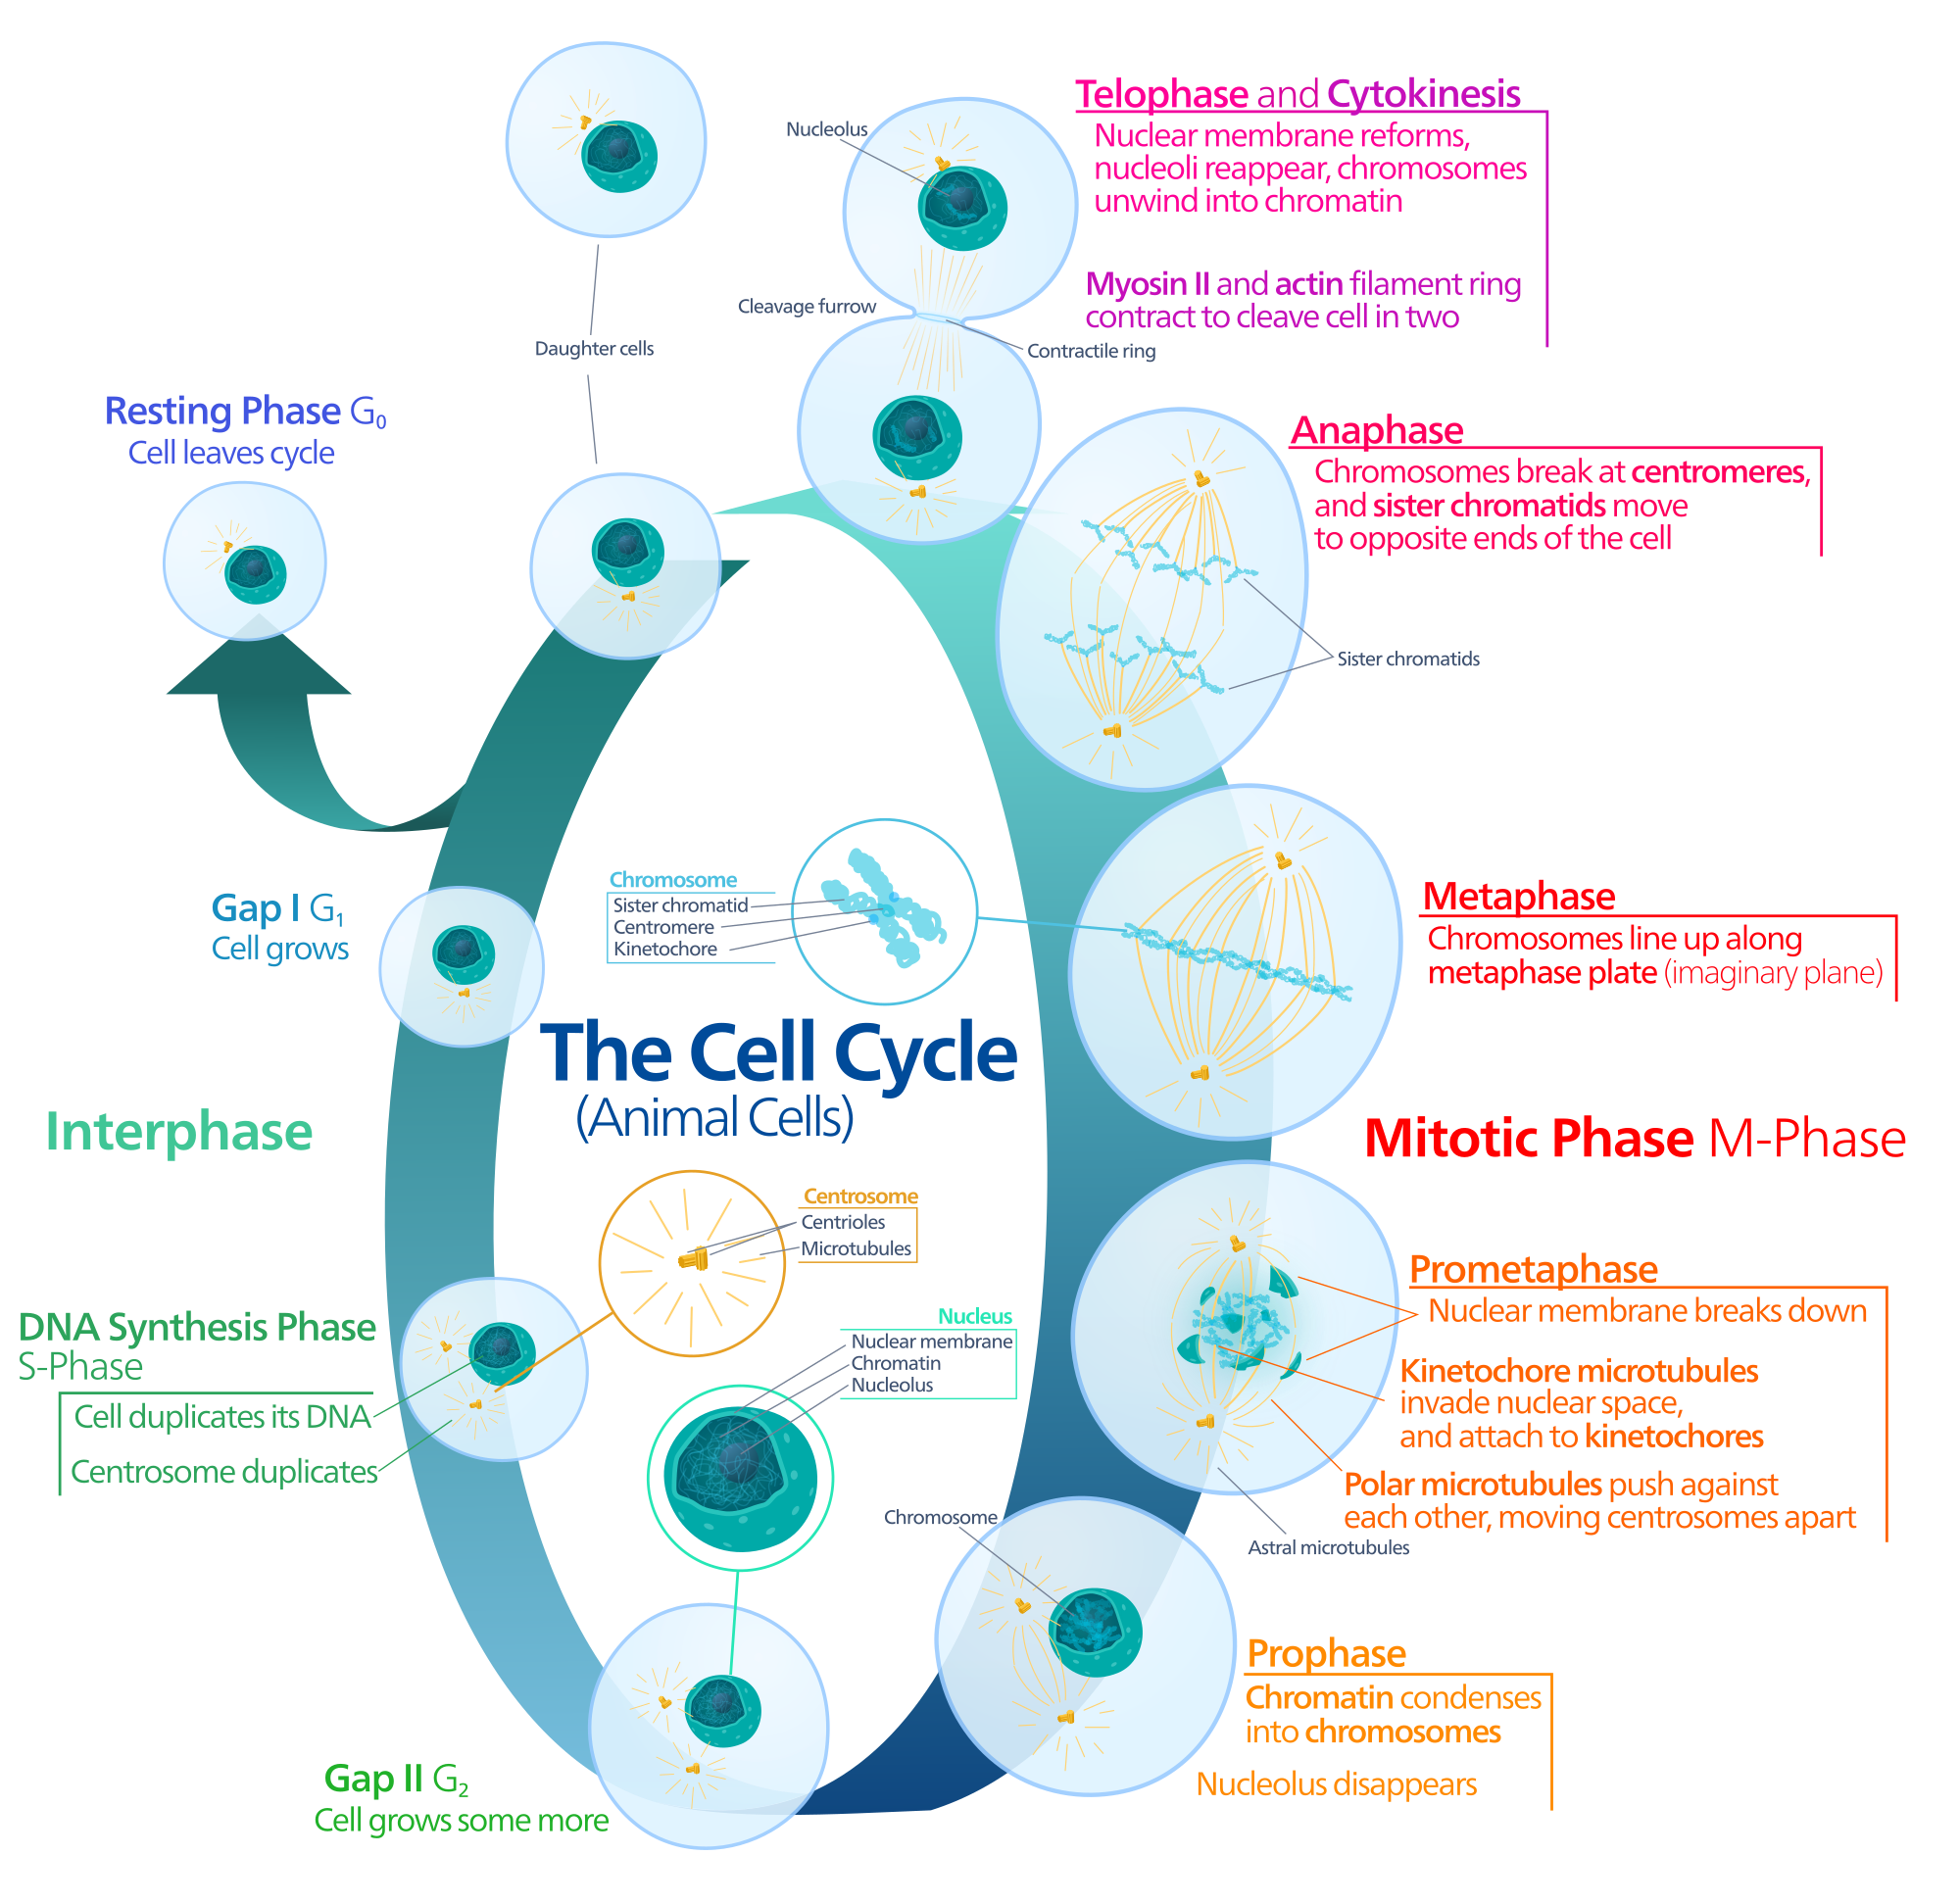
\includegraphics[width=0.7\linewidth]{./figures/reproduction/Animal_cell_cycle-en} 

}

\caption{\href{https://commons.wikimedia.org/wiki/File:Animal_cell_cycle-en.svg}{Mitosis in an animal cell (phases ordered counter-clockwise).}}\label{fig:cellcycle}
\end{figure}

The process of mitosis is divided into stages corresponding to the completion of one set of activities and the start of the next. These stages are prophase, prometaphase, metaphase, anaphase, and telophase. During mitosis, the chromosomes, which have already duplicated, condense and attach to spindle fibers that pull one copy of each chromosome to opposite sides of the cell. The result is two genetically identical daughter nuclei. The rest of the cell may then continue to divide by cytokinesis to produce two daughter cells. Producing three or more daughter cells instead of the normal two is a mitotic error called tripolar mitosis or multipolar mitosis (direct cell triplication / multiplication). Other errors during mitosis can induce apoptosis (programmed cell death) or cause mutations. Certain types of cancer can arise from such mutations.



\begin{figure}

{\centering 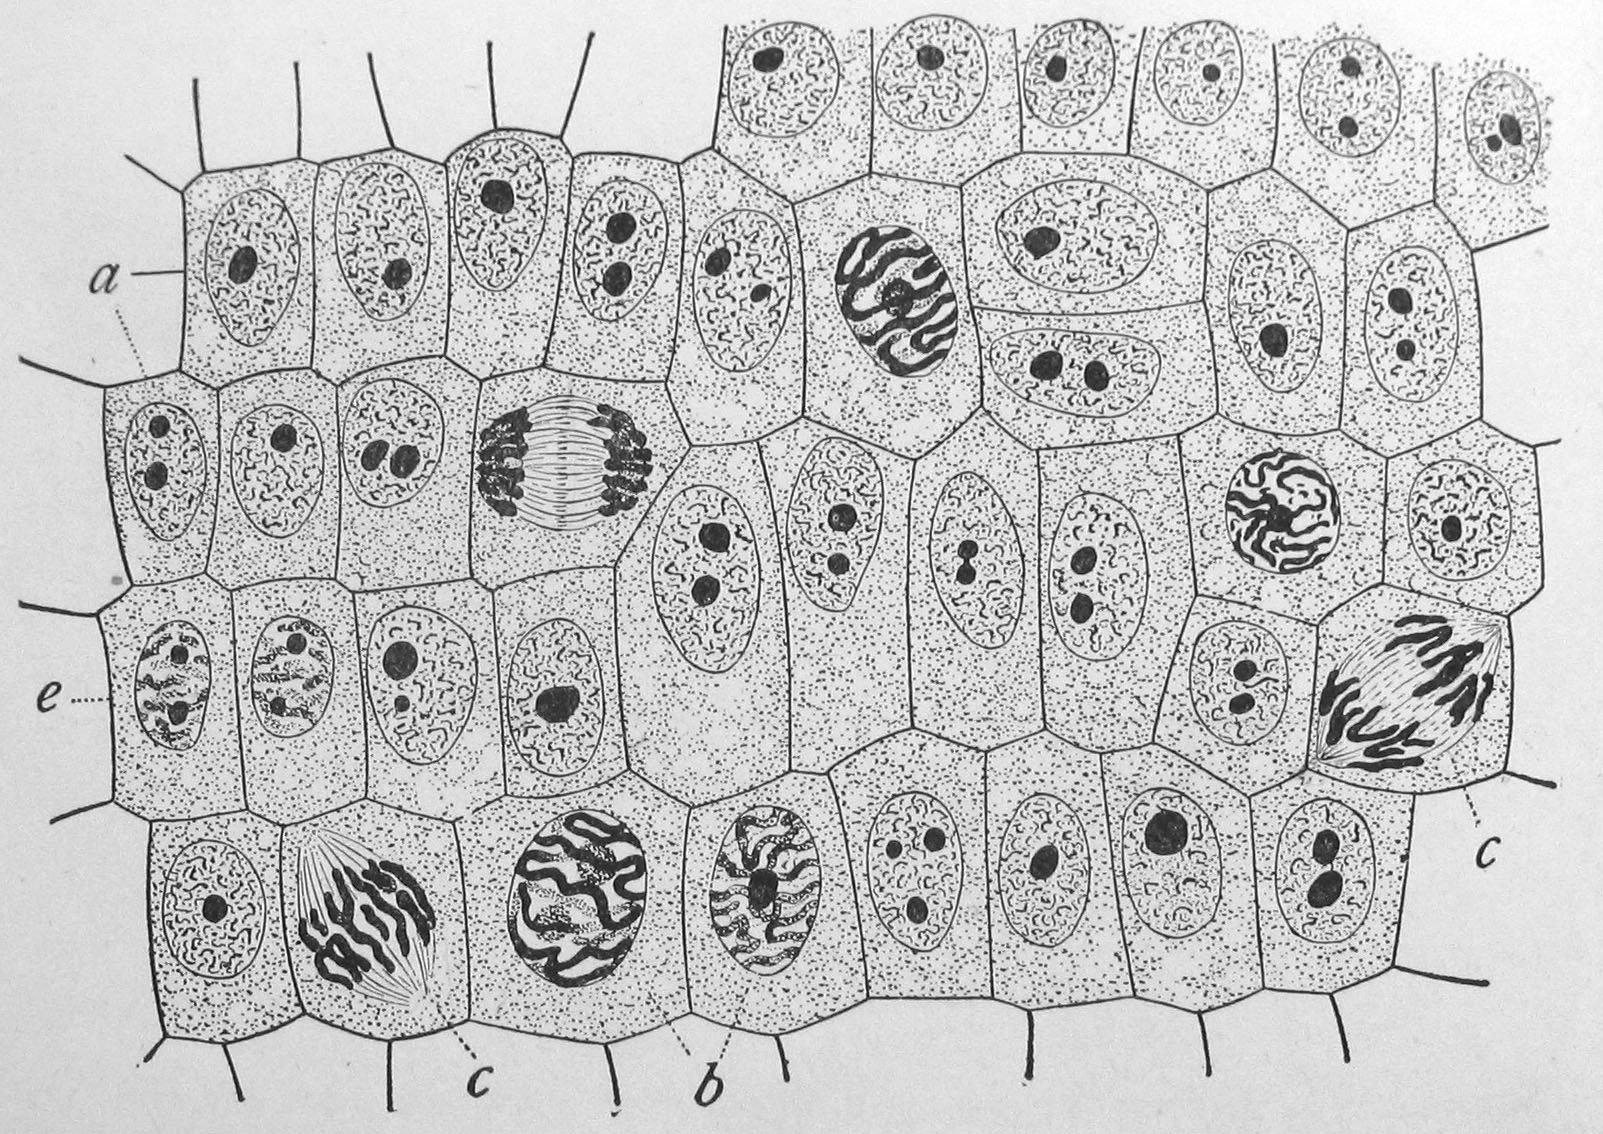
\includegraphics[width=0.7\linewidth]{./figures/reproduction/Wilson1900Fig2} 

}

\caption{Onion (Allium cepa) root cells in different phases of the cell cycle (drawn by \href{https://en.wikipedia.org/wiki/Edmund_Beecher_Wilson}{E. B. Wilson}, 1900). \href{https://commons.wikimedia.org/wiki/File:Wilson1900Fig2.jpg}{General view of cells in the growing root-tip of the onion, from a longitudinal section, enlarged 800 diameters. a. non-dividing cells, with chromatin-network and deeply stained nucleoli; b. nuclei preparing for division (spireme-stage); c. dividing cells showing mitotic figures; e. pair of daughter-cells shortly after division.}}\label{fig:onionroot}
\end{figure}

Mitosis varies between organisms. For example, animal cells undergo an ``open'' mitosis, where the nuclear envelope breaks down before the chromosomes separate, whereas fungi undergo a ``closed'' mitosis, where chromosomes divide within an intact cell nucleus. Most animal cells undergo a shape change, known as mitotic cell rounding, to adopt a near spherical morphology at the start of mitosis. Most human cells are produced by mitotic cell division. Important exceptions include the gametes -- sperm and egg cells -- which are produced by meiosis.

Numerous descriptions of cell division were made during 18th and 19th centuries, with various degrees of accuracy. In 1835, the German botanist Hugo von Mohl, described cell division in the green alga \emph{Cladophora glomerata}, stating that multiplication of cells occurs through cell division. In 1838, Matthias Jakob Schleiden affirmed that the formation of new cells in their interior was a general law for cell multiplication in plants, a view later rejected in favour of Mohl model, due to contributions of Robert Remak and others.

The term ``mitosis'', coined by Walther Flemming in 1882, is derived from the Greek word μίτος (mitos, ``warp thread''). There are some alternative names for the process, e.g., ``karyokinesis'' (nuclear division), a term introduced by Schleicher in 1878, or ``equational division'', proposed by August Weismann in 1887. However, the term ``mitosis'' is also used in a broad sense by some authors to refer to karyokinesis and cytokinesis together. Presently, ``equational division'' is more commonly used to refer to meiosis II, the part of meiosis most like mitosis.

The primary result of mitosis and cytokinesis is the transfer of a parent cell's genome into two daughter cells. The genome is composed of a number of chromosomes---complexes of tightly coiled DNA that contain genetic information vital for proper cell function. Because each resultant daughter cell should be genetically identical to the parent cell, the parent cell must make a copy of each chromosome before mitosis. This occurs during the S phase of interphase. Chromosome duplication results in two identical sister chromatids bound together by cohesin proteins at the centromere.

When mitosis begins, the chromosomes condense and become visible. In some eukaryotes, for example animals, the nuclear envelope, which segregates the DNA from the cytoplasm, disintegrates into small vesicles. The nucleolus also disappears. Microtubules project from opposite ends of the cell, attach to the centromeres, and align the chromosomes centrally within the cell. The microtubules then contract to pull the sister chromatids of each chromosome apart. Sister chromatids at this point are called daughter chromosomes. As the cell elongates, corresponding daughter chromosomes are pulled toward opposite ends of the cell and condense maximally in late anaphase. A new nuclear envelope forms around the separated daughter chromosomes, which decondense to form interphase nuclei.

During mitotic progression, typically after the anaphase onset, the cell may undergo cytokinesis. In animal cells, a cell membrane pinches inward between the two developing nuclei to produce two new cells. In plant cells, a cell plate forms between the two nuclei. Cytokinesis does not always occur; coenocytic (a type of multinucleate condition) cells undergo mitosis without cytokinesis.

\hypertarget{interphase}{%
\subsection{Interphase}\label{interphase}}

The mitotic phase is a relatively short period of the cell cycle. It alternates with the much longer interphase, where the cell prepares itself for the process of cell division. Interphase is divided into three phases: G1 (first gap), S (synthesis), and G2 (second gap). During all three parts of interphase, the cell grows by producing proteins and cytoplasmic organelles. However, chromosomes are replicated only during the S phase. Thus, a cell grows (G1), continues to grow as it duplicates its chromosomes (S), grows more and prepares for mitosis (G2), and finally divides (M) before restarting the cycle. All these phases in the cell cycle are highly regulated by cyclins, cyclin-dependent kinases, and other cell cycle proteins. The phases follow one another in strict order and there are ``checkpoints'' that give the cell cues to proceed from one phase to another. Cells may also temporarily or permanently leave the cell cycle and enter G0 phase to stop dividing. This can occur when cells become overcrowded (density-dependent inhibition) or when they differentiate to carry out specific functions for the organism, as is the case for human heart muscle cells and neurons. Some G0 cells have the ability to re-enter the cell cycle.

\hypertarget{preprophase-plant-cells}{%
\subsection{Preprophase (plant cells)}\label{preprophase-plant-cells}}

In plant cells only, prophase is preceded by a pre-prophase stage. In highly vacuolated plant cells, the nucleus has to migrate into the center of the cell before mitosis can begin. This is achieved through the formation of a phragmosome, a transverse sheet of cytoplasm that bisects the cell along the future plane of cell division. In addition to phragmosome formation, preprophase is characterized by the formation of a ring of microtubules and actin filaments (called preprophase band) underneath the plasma membrane around the equatorial plane of the future mitotic spindle. This band marks the position where the cell will eventually divide. The cells of higher plants (such as the flowering plants) lack centrioles; instead, microtubules form a spindle on the surface of the nucleus and are then organized into a spindle by the chromosomes themselves, after the nuclear envelope breaks down. The preprophase band disappears during nuclear envelope breakdown and spindle formation in prometaphase.:58--67

\hypertarget{prophase}{%
\subsection{Prophase}\label{prophase}}

During prophase, which occurs after G2 interphase, the cell prepares to divide by tightly condensing its chromosomes and initiating mitotic spindle formation. During interphase, the genetic material in the nucleus consists of loosely packed chromatin. At the onset of prophase, chromatin fibers condense into discrete chromosomes that are typically visible at high magnification through a light microscope. In this stage, chromosomes are long, thin and thread-like. Each chromosome has two chromatids. The two chromatids are joined at the centromere.

Gene transcription ceases during prophase and does not resume until late anaphase to early G1 phase. The nucleolus also disappears during early prophase.

Close to the nucleus of animal cells are structures called centrosomes, consisting of a pair of centrioles surrounded by a loose collection of proteins. The centrosome is the coordinating center for the cell's microtubules. A cell inherits a single centrosome at cell division, which is duplicated by the cell before a new round of mitosis begins, giving a pair of centrosomes. The two centrosomes polymerize tubulin to help form a microtubule spindle apparatus. Motor proteins then push the centrosomes along these microtubules to opposite sides of the cell. Although centrosomes help organize microtubule assembly, they are not essential for the formation of the spidle apparatus, since they are absent from plants, and are not absolutely required for animal cell mitosis.



\begin{figure}

{\centering 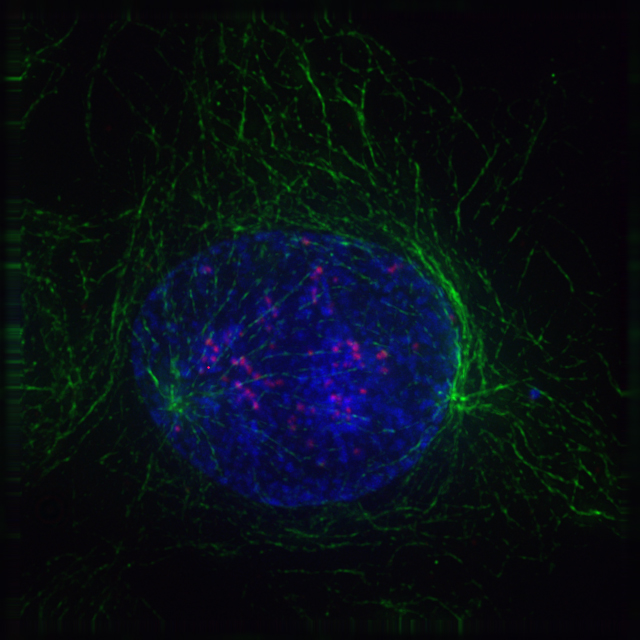
\includegraphics[width=0.7\linewidth]{./figures/reproduction/ProphaseIF} 

}

\caption{\href{https://commons.wikimedia.org/wiki/File:ProphaseIF.jpg}{Early prophase: Polar microtubules, shown as green strands, have established a matrix around the currently intact nucleus, with the condensing chromosomes in blue. The red nodules are the centromeres.}}\label{fig:prophase}
\end{figure}

\hypertarget{prometaphase}{%
\subsection{Prometaphase}\label{prometaphase}}

At the beginning of prometaphase in animal cells, phosphorylation of nuclear lamins causes the nuclear envelope to disintegrate into small membrane vesicles. As this happens, microtubules invade the nuclear space. This is called open mitosis, and it occurs in some multicellular organisms. Fungi and some protists, such as algae or trichomonads, undergo a variation called closed mitosis where the spindle forms inside the nucleus, or the microtubules penetrate the intact nuclear envelope.

In late prometaphase, kinetochore microtubules begin to search for and attach to chromosomal kinetochores. A kinetochore is a proteinaceous microtubule-binding structure that forms on the chromosomal centromere during late prophase. A number of polar microtubules find and interact with corresponding polar microtubules from the opposite centrosome to form the mitotic spindle. Although the kinetochore structure and function are not fully understood, it is known that it contains some form of molecular motor. When a microtubule connects with the kinetochore, the motor activates, using energy from ATP to ``crawl'' up the tube toward the originating centrosome. This motor activity, coupled with polymerisation and depolymerisation of microtubules, provides the pulling force necessary to later separate the chromosome's two chromatids.



\begin{figure}

{\centering 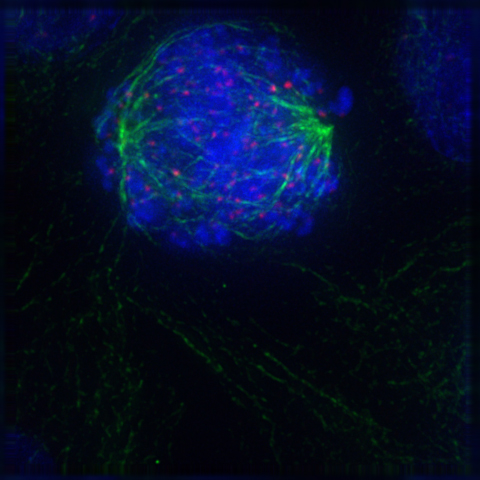
\includegraphics[width=0.7\linewidth]{./figures/reproduction/Prometaphase} 

}

\caption{\href{https://commons.wikimedia.org/wiki/File:Prometaphase.jpg}{Early prometaphase: The nuclear membrane has just disassembled, allowing the microtubules to quickly interact with the kinetochores, which assemble on the centromeres of the condensing chromosomes.}}\label{fig:prometaphase}
\end{figure}

\hypertarget{metaphase}{%
\subsection{Metaphase}\label{metaphase}}

After the microtubules have located and attached to the kinetochores in prometaphase, the two centrosomes begin pulling the chromosomes towards opposite ends of the cell. The resulting tension causes the chromosomes to align along the metaphase plate or equatorial plane, an imaginary line that is centrally located between the two centrosomes (at approximately the midline of the cell). To ensure equitable distribution of chromosomes at the end of mitosis, the metaphase checkpoint guarantees that kinetochores are properly attached to the mitotic spindle and that the chromosomes are aligned along the metaphase plate. If the cell successfully passes through the metaphase checkpoint, it proceeds to anaphase.



\begin{figure}

{\centering 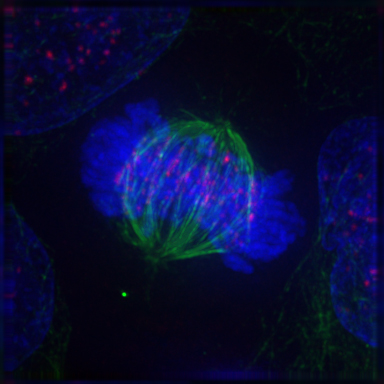
\includegraphics[width=0.7\linewidth]{./figures/reproduction/MetaphaseIF} 

}

\caption{\href{https://commons.wikimedia.org/wiki/File:MetaphaseIF.jpg}{Metaphase: The centrosomes have moved to the poles of the cell and have established the mitotic spindle. The chromosomes have congressed at the metaphase plate.}}\label{fig:metaphase}
\end{figure}

\hypertarget{anaphase}{%
\subsection{Anaphase}\label{anaphase}}

During anaphase A, the cohesins that bind sister chromatids together are cleaved, forming two identical daughter chromosomes. Shortening of the kinetochore microtubules pulls the newly formed daughter chromosomes to opposite ends of the cell. During anaphase B, polar microtubules push against each other, causing the cell to elongate. In late anaphase, chromosomes also reach their overall maximal condensation level, to help chromosome segregation and the re-formation of the nucleus. In most animal cells, anaphase A precedes anaphase B, but some vertebrate egg cells demonstrate the opposite order of events.



\begin{figure}

{\centering 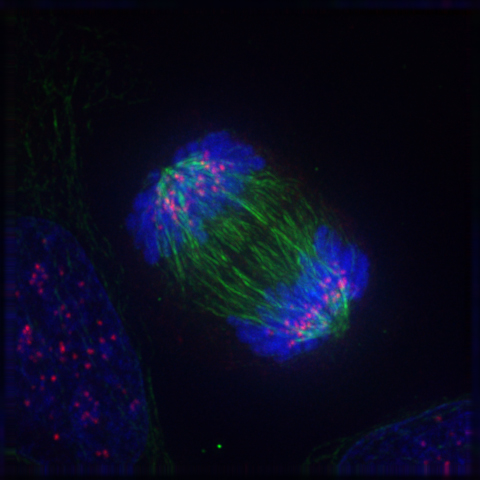
\includegraphics[width=0.7\linewidth]{./figures/reproduction/Anaphase_IF} 

}

\caption{\href{https://commons.wikimedia.org/wiki/File:Anaphase_IF.jpg}{Anaphase: Kinetochore microtubules pull the two sets of chromosomes apart, and lengthening polar microtubules push the halves of the dividing cell further apart, while chromosomes are condensed maximally.}}\label{fig:anaphase}
\end{figure}

\hypertarget{telophase}{%
\subsection{Telophase}\label{telophase}}

Telophase (from the Greek word τελος meaning ``end'') is a reversal of prophase and prometaphase events. At telophase, the polar microtubules continue to lengthen, elongating the cell even more. If the nuclear envelope has broken down, a new nuclear envelope forms using the membrane vesicles of the parent cell's old nuclear envelope. The new envelope forms around each set of separated daughter chromosomes (though the membrane does not enclose the centrosomes) and the nucleolus reappears. Both sets of chromosomes, now surrounded by new nuclear membrane, begin to ``relax'' or decondense. Mitosis is complete. Each daughter nucleus has an identical set of chromosomes.Cell division may or may not occur at this time depending on the organism.



\begin{figure}

{\centering 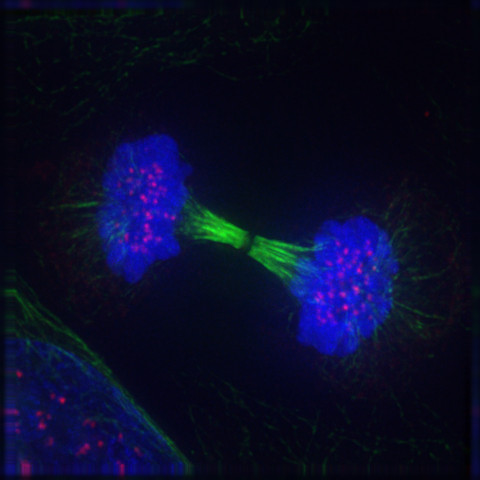
\includegraphics[width=0.7\linewidth]{./figures/reproduction/TelophaseIF} 

}

\caption{\href{https://commons.wikimedia.org/wiki/File:TelophaseIF.jpg}{Telophase: Reversal of prophase and prometaphase events and thus completing the cell cycle.}}\label{fig:telophase}
\end{figure}

\hypertarget{cytokinesis}{%
\subsection{Cytokinesis}\label{cytokinesis}}

Cytokinesis is not a phase of mitosis but rather a separate process, necessary for completing cell division. In animal cells, a cleavage furrow (pinch) containing a contractile ring develops where the metaphase plate used to be, pinching off the separated nuclei. In both animal and plant cells, cell division is also driven by vesicles derived from the Golgi apparatus, which move along microtubules to the middle of the cell. In plants, this structure coalesces into a cell plate at the center of the phragmoplast and develops into a cell wall, separating the two nuclei. Each daughter cell has a complete copy of the genome of its parent cell. The end of cytokinesis marks the end of the M-phase.

There are many cells where mitosis and cytokinesis occur separately, forming single cells with multiple nuclei. The most notable occurrence of this is among the fungi, slime molds, and coenocytic algae, but the phenomenon is found in various other organisms. Even in animals, cytokinesis and mitosis may occur independently, for instance during certain stages of fruit fly embryonic development.

Mitosis occurs in the following circumstances:

\begin{itemize}
\tightlist
\item
  Development and growth: The number of cells within an organism increases by mitosis. This is the basis of the development of a multicellular body from a single cell, i.e., zygote and also the basis of the growth of a multicellular body.
\item
  Cell replacement: In some parts of the body, e.g.~skin and digestive tract, cells are constantly sloughed off and replaced by new ones. New cells are formed by mitosis and so are exact copies of the cells being replaced.
\item
  Regeneration: Some organisms can regenerate body parts. The production of new cells in such instances is achieved by mitosis. For example, starfish regenerate lost arms through mitosis.
\item
  Asexual reproduction: Some organisms produce genetically similar offspring through asexual reproduction. For example, the hydra reproduces asexually by budding. The cells at the surface of hydra undergo mitosis and form a mass called a bud. Mitosis continues in the cells of the bud and this grows into a new individual. The same division happens during asexual reproduction or vegetative propagation in plants.
\end{itemize}

\hypertarget{meiosis}{%
\section{Meiosis}\label{meiosis}}

Meiosis (from Greek μείωσις, meiosis, which means lessening) is a special type of cell division that reduces the chromosome number by half, creating four haploid cells, each genetically distinct from the parent cell that gave rise to them. This process occurs in all sexually reproducing single-celled and multicellular eukaryotes, including animals, plants, and fungi. Meiotic cell divisions are an essential process during oogenesis and spermatogenesis.

Errors in meiosis resulting in aneuploidy are the leading known cause of miscarriage and the most frequent genetic cause of developmental disabilities.

In meiosis, DNA replication is followed by two rounds of cell division to produce four daughter cells, each with half the number of chromosomes as the original parent cell. The two meiotic divisions are known as Meiosis I and Meiosis II. Before meiosis begins, during S phase of the cell cycle, the DNA of each chromosome is replicated so that it consists of two identical sister chromatids, which remain held together through sister chromatid cohesion. This S-phase can be referred to as ``premeiotic S-phase'' or ``meiotic S-phase''. Immediately following DNA replication, meiotic cells enter a prolonged G2-like stage known as meiotic prophase. During this time, homologous chromosomes pair with each other and undergo genetic recombination, a programmed process in which DNA may be cut and then repaired, which allows them to exchange some of their genetic information. A subset of recombination events results in crossovers, which create physical links known as chiasmata (singular: chiasma, for the Greek letter Chi (X)) between the homologous chromosomes. In most organisms, these links can help direct each pair of homologous chromosomes to segregate away from each other during Meiosis I, resulting in two haploid cells that have half the number of chromosomes as the parent cell. During Meiosis II, the cohesion between sister chromatids is released and they segregate from one another, as during mitosis. In some cases all four of the meiotic products form gametes such as sperm, spores, or pollen. In female animals, three of the four meiotic products are typically eliminated by extrusion into polar bodies, and only one cell develops to produce an ovum. Because the number of chromosomes is halved during meiosis, gametes can fuse (i.e.~fertilization) to form a diploid zygote that contains two copies of each chromosome, one from each parent. Thus, alternating cycles of meiosis and fertilization enable sexual reproduction, with successive generations maintaining the same number of chromosomes. For example, diploid human cells contain 23 pairs of chromosomes including 1 pair of sex chromosomes (46 total), half of maternal origin and half of paternal origin. Meiosis produces haploid gametes (ova or sperm) that contain one set of 23 chromosomes. When two gametes (an egg and a sperm) fuse, the resulting zygote is once again diploid, with the mother and father each contributing 23 chromosomes. This same pattern, but not the same number of chromosomes, occurs in all organisms that utilize meiosis.

Meiosis begins with a diploid cell, which contains two copies of each chromosome, termed homologs. First, the cell undergoes DNA replication, so each homolog now consists of two identical sister chromatids. Then each set of homologs pair with each other and exchange genetic information by homologous recombination often leading to physical connections (crossovers) between the homologs. In the first meiotic division, the homologs are segregated to separate daughter cells by the spindle apparatus. The cells then proceed to a second division without an intervening round of DNA replication. The sister chromatids are segregated to separate daughter cells to produce a total of four haploid cells. Female animals employ a slight variation on this pattern and produce one large ovum and two small polar bodies. Because of recombination, an individual chromatid can consist of a new combination of maternal and paternal genetic information, resulting in offspring that are genetically distinct from either parent. Furthermore, an individual gamete can include an assortment of maternal, paternal, and recombinant chromatids. This genetic diversity resulting from sexual reproduction contributes to the variation in traits upon which natural selection can act.

Meiosis uses many of the same mechanisms as mitosis, the type of cell division used by eukaryotes to divide one cell into two identical daughter cells. In some plants, fungi, and protists meiosis results in the formation of spores: haploid cells that can divide vegetatively without undergoing fertilization. Some eukaryotes, like bdelloid rotifers, do not have the ability to carry out meiosis and have acquired the ability to reproduce by parthenogenesis.

Meiosis does not occur in archaea or bacteria, which generally reproduce asexually via binary fission. However, a ``sexual'' process known as horizontal gene transfer involves the transfer of DNA from one bacterium or archaeon to another and recombination of these DNA molecules of different parental origin.

Meiosis was discovered and described for the first time in sea urchin eggs in 1876 by the German biologist Oscar Hertwig. It was described again in 1883, at the level of chromosomes, by the Belgian zoologist Edouard Van Beneden, in Ascaris roundworm eggs. The significance of meiosis for reproduction and inheritance, however, was described only in 1890 by German biologist August Weismann, who noted that two cell divisions were necessary to transform one diploid cell into four haploid cells if the number of chromosomes had to be maintained. In 1911 the American geneticist Thomas Hunt Morgan detected crossovers in meiosis in the fruit fly Drosophila melanogaster, which helped to establish that genetic traits are transmitted on chromosomes.

The term ``meiosis'' (originally spelled ``maiosis'') is derived from the Greek word μείωσις, meaning `lessening'. It was introduced to biology by J.B. Farmer and J.E.S. Moore in 1905:

``We propose to apply the terms Maiosis or Maiotic phase to cover the whole series of nuclear changes included in the two divisions that were designated as Heterotype and Homotype by Flemming.''

The term was linguistically corrected to ``meiosis'' by Koernicke (1905), and by Pantel and De Sinety (1906).

Meiosis is divided into meiosis I and meiosis II which are further divided into Karyokinesis I and Cytokinesis I and Karyokinesis II and Cytokinesis II respectively. The preparatory steps that lead up to meiosis are identical in pattern and name to interphase of the mitotic cell cycle. Interphase is divided into three phases:

\begin{itemize}
\tightlist
\item
  Growth 1 (G1) phase: In this very active phase, the cell synthesizes its vast array of proteins, including the enzymes and structural proteins it will need for growth. In G1, each of the chromosomes consists of a single linear molecule of DNA.
\item
  Synthesis (S) phase: The genetic material is replicated; each of the cell's chromosomes duplicates to become two identical sister chromatids attached at a centromere. This replication does not change the ploidy of the cell since the centromere number remains the same. The identical sister chromatids have not yet condensed into the densely packaged chromosomes visible with the light microscope. This will take place during prophase I in meiosis.
\item
  Growth 2 (G2) phase: G2 phase as seen before mitosis is not present in meiosis. Meiotic prophase corresponds most closely to the G2 phase of the mitotic cell cycle.
\end{itemize}

Interphase is followed by meiosis I and then meiosis II. Meiosis I separates replicated homologous chromosomes, each still made up of two sister chromatids, into two daughter cells, thus reducing the chromosome number by half. During meiosis II, sister chromatids decouple and the resultant daughter chromosomes are segregated into four daughter cells. For diploid organisms, the daughter cells resulting from meiosis are haploid and contain only one copy of each chromosome. In some species, cells enter a resting phase known as interkinesis between meiosis I and meiosis II.

Meiosis I and II are each divided into prophase, metaphase, anaphase, and telophase stages, similar in purpose to their analogous subphases in the mitotic cell cycle. Therefore, meiosis includes the stages of meiosis I (prophase I, metaphase I, anaphase I, telophase I) and meiosis II (prophase II, metaphase II, anaphase II, telophase II).

Meiosis generates gamete genetic diversity in two ways: (1) Law of Independent Assortment. The independent orientation of homologous chromosome pairs along the metaphase plate during metaphase I \& orientation of sister chromatids in metaphase II, this is the subsequent separation of homologs and sister chromatids during anaphase I \& II, it allows a random and independent distribution of chromosomes to each daughter cell (and ultimately to gametes); and (2) Crossing Over. The physical exchange of homologous chromosomal regions by homologous recombination during prophase I results in new combinations of genetic information within chromosomes.

During meiosis, specific genes are more highly transcribed. In addition to strong meiotic stage-specific expression of mRNA, there are also pervasive translational controls (e.g.~selective usage of preformed mRNA), regulating the ultimate meiotic stage-specific protein expression of genes during meiosis. Thus, both transcriptional and translational controls determine the broad restructuring of meiotic cells needed to carry out meiosis.

\hypertarget{meiosis-i}{%
\subsection{Meiosis I}\label{meiosis-i}}

Meiosis I segregates homologous chromosomes, which are joined as tetrads (2n, 4c), producing two haploid cells (n chromosomes, 23 in humans) which each contain chromatid pairs (1n, 2c). Because the ploidy is reduced from diploid to haploid, meiosis I is referred to as a reductional division. Meiosis II is an equational division analogous to mitosis, in which the sister chromatids are segregated, creating four haploid daughter cells (1n, 1c).

\hypertarget{prophase-i}{%
\subsubsection{Prophase I}\label{prophase-i}}

Prophase I is typically the longest phase of meiosis. During prophase I, homologous chromosomes pair and exchange genetic information (homologous recombination). This often results in chromosomal crossover. This process facilitates pairing between homologous chromosomes and hence accurate segregation of the chromosomes at the first meiosis division. The new combinations of DNA created during crossover are a significant source of genetic variation, and result in new combinations of alleles, which may be beneficial. The paired and replicated chromosomes are called bivalents or tetrads, which have two chromosomes and four chromatids, with one chrmosome coming from each parent. The process of pairing the homologous chromosomes is called synapsis. At this stage, non-sister chromatids may cross-over at points called chiasmata (plural; singular chiasma). Prophase I has historically been divided into a series of substages which are named according to the appearance of chromosomes.

\hypertarget{leptotene}{%
\paragraph{Leptotene}\label{leptotene}}

The first stage of prophase I is the leptotene stage, also known as leptonema, from Greek words meaning ``thin threads''. In this stage of prophase I, individual chromosomes---each consisting of two sister chromatids---become ``individualized'' to form visible strands within the nucleus. The two sister chromatids closely associate and are visually indistinguishable from one another. During leptotene, lateral elements of the synaptonemal complex assemble. Leptotene is of very short duration and progressive condensation and coiling of chromosome fibers takes place.

\hypertarget{zygotene}{%
\paragraph{Zygotene}\label{zygotene}}

The zygotene stage, also known as zygonema, from Greek words meaning ``paired threads'', occurs as the chromosomes approximately line up with each other into homologous chromosome pairs. In some organisms, this is called the bouquet stage because of the way the telomeres cluster at one end of the nucleus. At this stage, the synapsis (pairing/coming together) of homologous chromosomes takes place, facilitated by assembly of central element of the synaptonemal complex. Pairing is brought about in a zipper-like fashion and may start at the centromere (procentric), at the chromosome ends (proterminal), or at any other portion (intermediate). Individuals of a pair are equal in length and in position of the centromere. Thus pairing is highly specific and exact. The paired chromosomes are called bivalent or tetrad chromosomes.

\hypertarget{pachytene}{%
\paragraph{Pachytene}\label{pachytene}}

The pachytene stage, also known as pachynema, from Greek words meaning ``thick threads''. At this point a tetrad of the chromosomes has formed known as a bivalent. This is the stage when homologous recombination, including chromosomal crossover (crossing over), occurs. Nonsister chromatids of homologous chromosomes may exchange genetic information over regions of homology. Sex chromosomes, however, are not wholly identical, and only exchange information over a small region of homology. At the sites where exchange happens, chiasmata form. The exchange of information between the non-sister chromatids results in a recombination of information; each chromosome has the complete set of information it had before, and there are no gaps formed as a result of the process. Because the chromosomes cannot be distinguished in the synaptonemal complex, the actual act of crossing over is not perceivable through the microscope, and chiasmata are not visible until the next stage.

\hypertarget{diplotene}{%
\paragraph{Diplotene}\label{diplotene}}

During the diplotene stage, also known as diplonema, from Greek words meaning ``two threads'', the synaptonemal complex degrades and homologous chromosomes separate from one another a little. The chromosomes themselves uncoil a bit, allowing some transcription of DNA. However, the homologous chromosomes of each bivalent remain tightly bound at chiasmata, the regions where crossing-over occurred. The chiasmata remain on the chromosomes until they are severed at the transition to anaphase I.

In human fetal oogenesis, all developing oocytes develop to this stage and are arrested in prophase I before birth. This suspended state is referred to as the dictyotene stage or dictyate. It lasts until meiosis is resumed to prepare the oocyte for ovulation, which happens at puberty or even later.

\hypertarget{diakinesis}{%
\paragraph{Diakinesis}\label{diakinesis}}

Chromosomes condense further during the diakinesis stage, from Greek words meaning ``moving through''. This is the first point in meiosis where the four parts of the tetrads are actually visible. Sites of crossing over entangle together, effectively overlapping, making chiasmata clearly visible. Other than this observation, the rest of the stage closely resembles prometaphase of mitosis; the nucleoli disappear, the nuclear membrane disintegrates into vesicles, and the meiotic spindle begins to form.

During these stages, two centrosomes, containing a pair of centrioles in animal cells, migrate to the two poles of the cell. These centrosomes, which were duplicated during S-phase, function as microtubule organizing centers nucleating microtubules, which are essentially cellular ropes and poles. The microtubules invade the nuclear region after the nuclear envelope disintegrates, attaching to the chromosomes at the kinetochore. The kinetochore functions as a motor, pulling the chromosome along the attached microtubule toward the originating centrosome, like a train on a track. There are four kinetochores on each tetrad, but the pair of kinetochores on each sister chromatid fuses and functions as a unit during meiosis I.

\hypertarget{metaphase-i}{%
\subsubsection{Metaphase I}\label{metaphase-i}}

Homologous pairs move together along the metaphase plate: As kinetochore microtubules from both centrosomes attach to their respective kinetochores, the paired homologous chromosomes align along an equatorial plane that bisects the spindle, due to continuous counterbalancing forces exerted on the bivalents by the microtubules emanating from the two kinetochores of homologous chromosomes. This attachment is referred to as a bipolar attachment. The physical basis of the independent assortment of chromosomes is the random orientation of each bivalent along the metaphase plate, with respect to the orientation of the other bivalents along the same equatorial line. The protein complex cohesin holds sister chromatids together from the time of their replication until anaphase. In mitosis, the force of kinetochore microtubules pulling in opposite directions creates tension. The cell senses this tension and does not progress with anaphase until all the chromosomes are properly bi-oriented. In meiosis, establishing tension ordinarily requires at least one crossover per chromosome pair in addition to cohesin between sister chromatids (see Chromosome segregation).

\hypertarget{anaphase-i}{%
\subsubsection{Anaphase I}\label{anaphase-i}}

Kinetochore microtubules shorten, pulling homologous chromosomes (which each consist of a pair of sister chromatids) to opposite poles. Nonkinetochore microtubules lengthen, pushing the centrosomes farther apart. The cell elongates in preparation for division down the center. Unlike in mitosis, only the cohesin from the chromosome arms is degraded while the cohesin surrounding the centromere remains protected by a protein named Shugoshin (Japanese for ``guardian spirit''), what prevents the sister chromatids from separating. This allows the sister chromatids to remain together while homologs are segregated.

\hypertarget{telophase-i}{%
\subsubsection{Telophase I}\label{telophase-i}}

The first meiotic division effectively ends when the chromosomes arrive at the poles. Each daughter cell now has half the number of chromosomes but each chromosome consists of a pair of chromatids. The microtubules that make up the spindle network disappear, and a new nuclear membrane surrounds each haploid set. The chromosomes uncoil back into chromatin. Cytokinesis, the pinching of the cell membrane in animal cells or the formation of the cell wall in plant cells, occurs, completing the creation of two daughter cells. Sister chromatids remain attached during telophase I.

Cells may enter a period of rest known as interkinesis or interphase II. No DNA replication occurs during this stage.

\hypertarget{meiosis-ii}{%
\subsection{Meiosis II}\label{meiosis-ii}}

Meiosis II is the second meiotic division, and usually involves equational segregation, or separation of sister chromatids. Mechanically, the process is similar to mitosis, though its genetic results are fundamentally different. The end result is production of four haploid cells (n chromosomes, 23 in humans) from the two haploid cells (with n chromosomes, each consisting of two sister chromatids) produced in meiosis I. The four main steps of meiosis II are: prophase II, metaphase II, anaphase II, and telophase II.

In prophase II we see the disappearance of the nucleoli and the nuclear envelope again as well as the shortening and thickening of the chromatids. Centrosomes move to the polar regions and arrange spindle fibers for the second meiotic division.

In metaphase II, the centromeres contain two kinetochores that attach to spindle fibers from the centrosomes at opposite poles. The new equatorial metaphase plate is rotated by 90 degrees when compared to meiosis I, perpendicular to the previous plate.

This is followed by anaphase II, in which the remaining centromeric cohesin, not protected by Shugoshin anymore, is cleaved, allowing the sister chromatids to segregate. The sister chromatids by convention are now called sister chromosomes as they move toward opposing poles.

The process ends with telophase II, which is similar to telophase I, and is marked by decondensation and lengthening of the chromosomes and the disassembly of the spindle. Nuclear envelopes re-form and cleavage or cell plate formation eventually produces a total of four daughter cells, each with a haploid set of chromosomes.

Meiosis is now complete and ends up with four new daughter cells.

Meiosis occurs in eukaryotic life cycles involving sexual reproduction, consisting of the constant cyclical process of meiosis and fertilization. This takes place alongside normal mitotic cell division. In multicellular organisms, there is an intermediary step between the diploid and haploid transition where the organism grows. At certain stages of the life cycle, germ cells produce gametes. Somatic cells make up the body of the organism and are not involved in gamete production.

Cycling meiosis and fertilization events produces a series of transitions back and forth between alternating haploid and diploid states. The organism phase of the life cycle can occu either during the diploid state (diplontic life cycle), during the haploid state (haplontic life cycle), or both (haplodiplontic life cycle, in which there are two distinct organism phases, one during the haploid state and the other during the diploid state).

In the diplontic life cycle (with pre-gametic meiosis), of which humans are a part, the organism is diploid, grown from a diploid cell called the zygote. The organism's diploid germ-line stem cells undergo meiosis to create haploid gametes (the spermatozoa for males and ova for females), which fertilize to form the zygote. The diploid zygote undergoes repeated cellular division by mitosis to grow into the organism.

In the haplontic life cycle (with post-zygotic meiosis), the organism is haploid instead, spawned by the proliferation and differentiation of a single haploid cell called the gamete. Two organisms of opposing sex contribute their haploid gametes to form a diploid zygote. The zygote undergoes meiosis immediately, creating four haploid cells. These cells undergo mitosis to create the organism. Many fungi and many protozoa utilize the haplontic life cycle.{[}citation needed{]}

Finally, in the haplodiplontic life cycle (with sporic or intermediate meiosis), the living organism alternates between haploid and diploid states. Consequently, this cycle is also known as the alternation of generations. The diploid organism's germ-line cells undergo meiosis to produce spores. The spores proliferate by mitosis, growing into a haploid organism. The haploid organism's gamete then combines with another haploid organism's gamete, creating the zygote. The zygote undergoes repeated mitosis and differentiation to become a diploid organism again. The haplodiplontic life cycle can be considered a fusion of the diplontic and haplontic life cycles.

\hypertarget{nondisjunction}{%
\subsection{Nondisjunction}\label{nondisjunction}}

The normal separation of chromosomes in meiosis I or sister chromatids in meiosis II is termed disjunction. When the segregation is not normal, it is called nondisjunction. This results in the production of gametes which have either too many or too few of a particular chromosome, and is a common mechanism for trisomy or monosomy. Nondisjunction can occur in the meiosis I or meiosis II, phases of cellular reproduction, or during mitosis.

Most monosomic and trisomic human embryos are not viable, but some aneuploidies can be tolerated, such as trisomy for the smallest chromosome, chromosome 21. Phenotypes of thes aneuploidies range from severe developmental disorders to asymptomatic. Medical conditions include but are not limited to:

\begin{itemize}
\tightlist
\item
  Down syndrome -- trisomy of chromosome 21
\item
  Patau syndrome -- trisomy of chromosome 13
\item
  Edwards syndrome -- trisomy of chromosome 18
\item
  Klinefelter syndrome -- extra X chromosomes in males -- i.e.~XXY, XXXY, XXXXY, etc.
\item
  Turner syndrome -- lacking of one X chromosome in females -- i.e.~X0
\item
  Triple X syndrome -- an extra X chromosome in females
\item
  XYY syndrome -- an extra Y chromosome in males.
\end{itemize}

The probability of nondisjunction in human oocytes increases with increasing maternal age, presumably due to loss of cohesin over time.



\chapter{Mendelian Inheritance}\label{mendelian-inheritance}

\href{https://en.wikipedia.org/wiki/Mendelian_inheritance}{Mendelian inheritance} is a type of biological inheritance that follows the principles originally proposed by \href{https://en.wikipedia.org/wiki/Gregor_Mendel}{Gregor Mendel} in 1865 and 1866, re-discovered in 1900 and popularised by \href{https://en.wikipedia.org/wiki/William_Bateson}{William Bateson}. These principles were initially controversial. When Mendel's theories were integrated with the Boveri--Sutton chromosome theory of inheritance by \href{https://en.wikipedia.org/wiki/Thomas_Hunt_Morgan}{Thomas Hunt Morgan} in 1915, they became the core of classical genetics. \href{https://en.wikipedia.org/wiki/Ronald_Fisher}{Ronald Fisher} combined these ideas with the theory of natural selection in his 1930 book The Genetical Theory of Natural Selection, putting evolution onto a mathematical footing and forming the basis for population genetics within the modern evolutinary synthesis.



\begin{figure}

{\centering 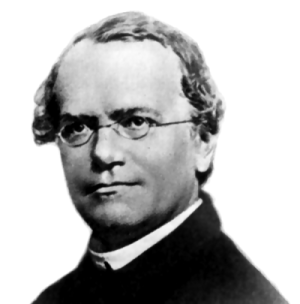
\includegraphics[width=0.7\linewidth]{./figures/mendel/Gregor_Mendel} 

}

\caption{\href{https://commons.wikimedia.org/wiki/File:Gregor_Mendel.png}{Gregor Mendel, the Moravian Augustinian monk who is credited for having founded the modern science of genetics}}\label{fig:portrait}
\end{figure}

The principles of Mendelian inheritance were named for and first derived by Gregor Johann Mendel, a nineteenth-century Moravian monk who formulated his ideas after conducting simple hybridisation experiments with pea plants (\emph{Pisum sativum}) he had planted in the garden of his monastery. Between 1856 and 1863, Mendel cultivated and tested some 5,000 pea plants. From these experiments, he induced two generalizations which later became known as Mendel's Principles of Heredity or Mendelian inheritance. He described his experiments in a two-part paper, Versuche über Pflanzen-Hybriden (Experiments on Plant Hybridization), that he presented to the Natural History Society of Brno on 8 February and 8 March 1865, and which was published in 1866.

Mendel's results were largely ignored. Although they were not completely unknown to biologists of the time, they were not seen as generally applicable, even by Mendel himself, who thought they only applied to certain categories of species or traits. A major block to understanding their significance was the importance attached by 19th-century biologists to the apparent blending of many inherited traits in the overall appearance of the progeny, now known to be due to multi-gene interactions, in contrast to the organ-specific binary characters studied by Mendel. In 1900, however, his work was ``re-discovered'' by three European scientists, \href{https://en.wikipedia.org/wiki/Hugo_de_Vries}{Hugo de Vries}, \href{https://en.wikipedia.org/wiki/Carl_Correns}{Carl Correns}, and \href{https://en.wikipedia.org/wiki/Erich_von_Tschermak}{Erich von Tschermak}. The exact nature of the ``re-discovery'' has been debated: De Vries published first on the subject, mentioning Mendel in a footnote, while Correns pointed out Mendel's priority after having read De Vries' paper and realizing that he himself did not have priority. De Vries may not have acknowledged truthfully how much of his knowledge of the laws came from his own work and how much came only after reading Mendel's paper. Later scholars have accused Von Tschermak of not truly understanding the results at all.

Regardless, the ``re-discovery'' made Mendelism an important but controversial theory. Its most vigorous promoter in Europe was William Bateson, who coined the terms ``genetics'' and ``allele'' to describe many of its tenets. The model of heredity was contested by other biologists because it implied that heredity was discontinuous, in opposition to the apparently continuous variation observable for many traits. Many biologists also dismissed the theory because they were not sure it would apply to all species. However, later work by biologists and statisticians such as Ronald Fisher showed that if multiple Mendelian factors were involved in the expression of an individual trait, they could produce the diverse results observed, and thus showed that Mendelian genetics is compatible with natural selection. Thomas Hunt Morgan and his assistants later integrated Mendel's theoretical model with the chromosome theory of inheritance, in which the chromosomes of cells were thought to hold the actual hereditary material, and created what is now known as classical genetics, a highly successful foundation which eventually cemented Mendel's place in history.

Mendel's findings allowed scientists such as Fisher and \href{https://en.wikipedia.org/wiki/J._B._S._Haldane}{J.B.S. Haldane} to predict the expression of traits on the basis of mathematical probabilities. An important aspect of Mendel's success can be traced to his decision to start his crosses only with plants he demonstrated were true-breeding. He only measured discrete (binary) characteristics, such as color, shape, and position of the seeds, rather than quantitatively variable characteristics. He expressed his results numerically and subjected them to statistical analysis. His method of data analysis and his large sample size gave credibility to his data. He had the foresight to follow several successive generations (P, F1, F2, F3) of pea plants and record their variations. Finally, he performed ``test crosses'' (backcrossing descendants of the initial hybridization to the initial true-breeding lines) to reveal the presence and proportions of recessive characters.

\hypertarget{mendels-genetic-discoveries}{%
\section{Mendel's genetic discoveries}\label{mendels-genetic-discoveries}}

Five parts of Mendel's discoveries were an important divergence from the common theories at the time and were the prerequisite for the establishment of his rules.

\begin{itemize}
\tightlist
\item
  Characters are unitary. That is, they are discrete (purple vs.~white, tall vs.~dwarf).
\item
  Genetic characteristics have alternate forms, each inherited from one of two parents. Today, we call these alleles.
\item
  One allele is dominant over the other. The phenotype reflects the dominant allele.
\item
  Gametes are created by random segregation. Heterozygotic individuals produce gametes with an equal frequency of the two alleles.
\item
  Different traits have independent assortment. In modern terms, genes are unlinked.
\end{itemize}

According to customary terminology we refer here to the principles of inheritance discovered by Gregor Mendel as Mendelian laws, although today's geneticists also speak of Mendelian rules or Mendelian principles, as there are many exceptions summarized under the collective term Non-Mendelian inheritance.

Mendel selected for experiment relate the following characters of pea plants:

\begin{itemize}
\tightlist
\item
  Form of the ripe seeds round or roundish, surface shallow or wrinkled
\item
  Colour of the seed--coat white, gray, brown with or without violet spotting
\item
  Colour of the seeds and cotyledons yellow or green
\item
  Flower colour
\item
  Form of the ripe pods simply inflated, not contracted or constricted between the seeds and wrinkled
\item
  Colour of the unripe pods yellow or green
\item
  Position of the flowers axial or terminal
\item
  Length of the stem
\end{itemize}



\begin{figure}

{\centering 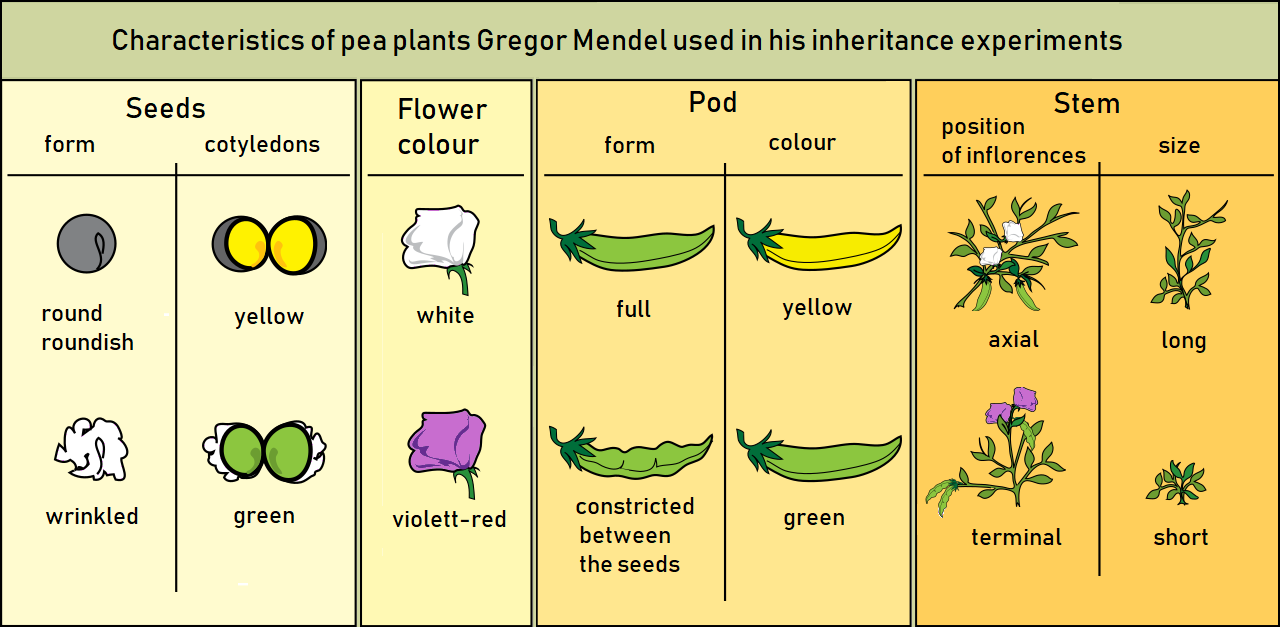
\includegraphics[width=0.7\linewidth]{./figures/mendel/Gregor_Mendel_-_characteristics_of_pea_plants_-_english} 

}

\caption{\href{https://commons.wikimedia.org/wiki/File:Gregor_Mendel_-_characteristics_of_pea_plants_-_english.png}{Characteristics of pea plants Gregor Mendel used in his inheritance experiments}}\label{fig:characteristics}
\end{figure}

When he crossed purebred white flower and purple flower pea plants (the parental or P generation) by artificial pollination, the resulting flower colour was not a blend. Rather than being a mix of the two, the offspring in the first generation (F1-generation) were all purple flowered. Therefore he called this biological trait dominant. When he allowed self-fertilization in the uniform looking F1-generation, he obtained both colours in the F2 generation with a purple flower to white flower ratio of 3 : 1. In some of the other characters also one of the traits was dominant.



\begin{figure}

{\centering 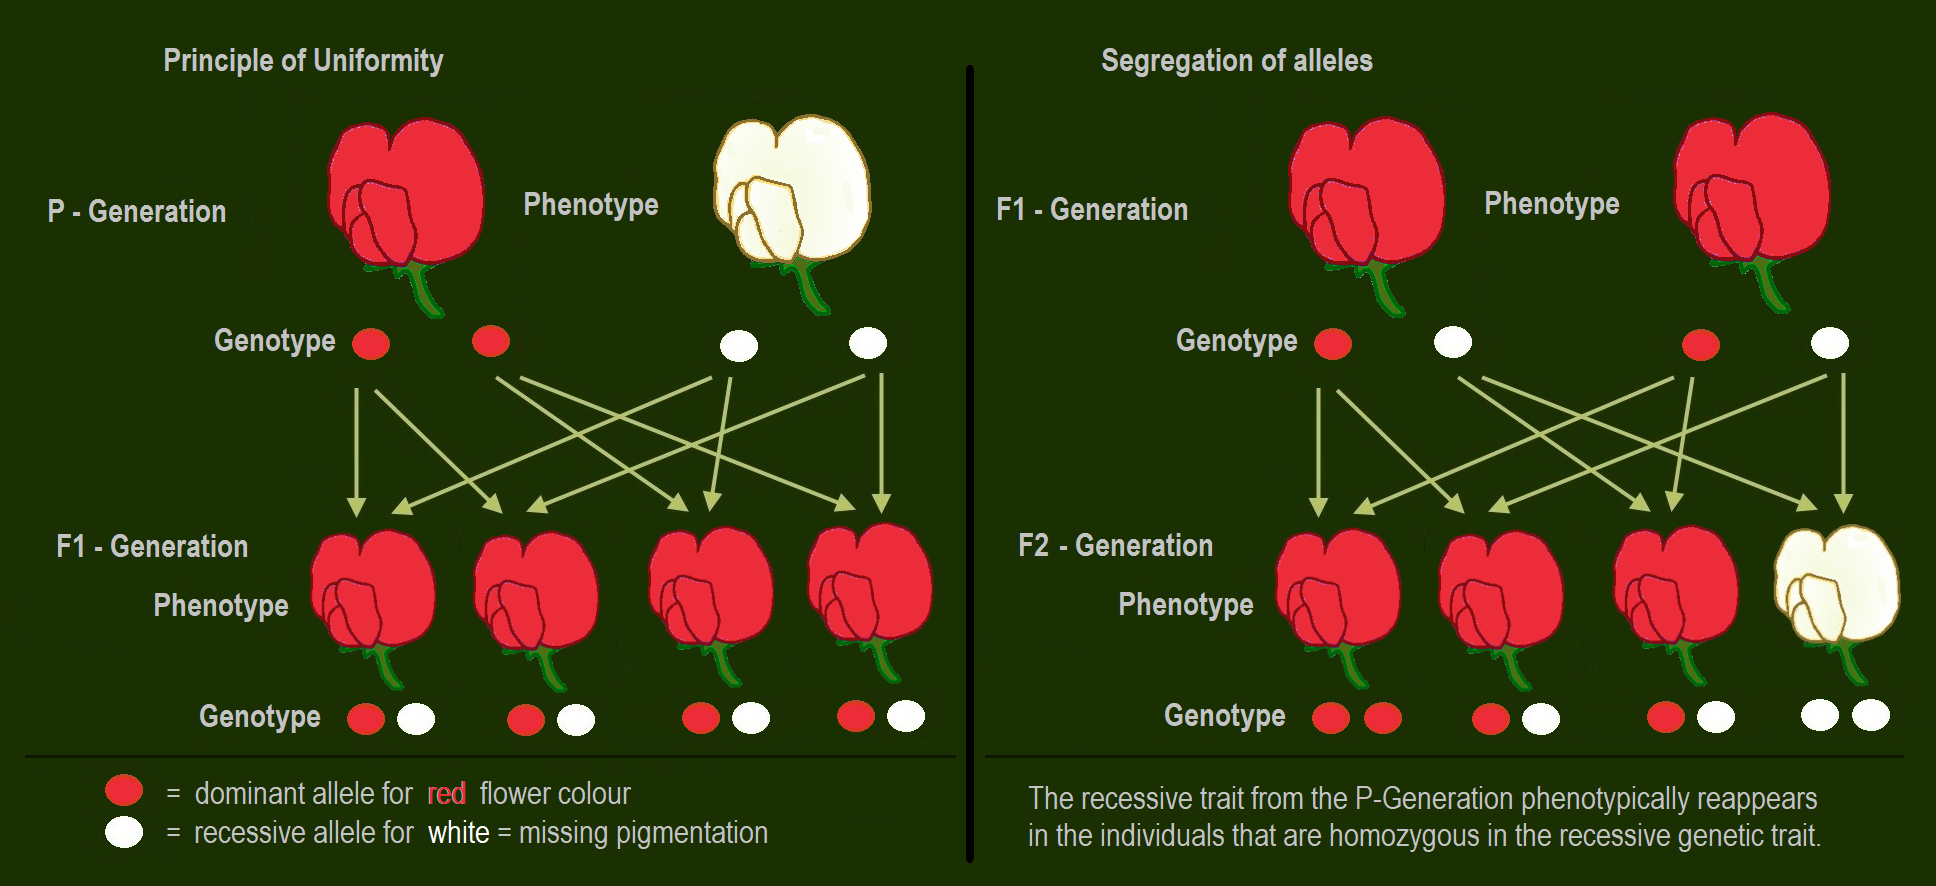
\includegraphics[width=0.7\linewidth]{./figures/mendel/Dominant-recessive_inheritance_-_flowers_of_pea_plants} 

}

\caption{\href{https://commons.wikimedia.org/wiki/File:Dominant-recessive_inheritance_-_flowers_of_pea_plants.png}{P-Generation and F1-Generation: The dominant allele for purple-red flower hides the phenotypic effect of the recessive allele for white flowers. F2-Generation: The recessive trait from the P-Generation phenotypically reappears in the individuals that are homozygous with the recessiv genetic trait.}}\label{fig:dominant}
\end{figure}

He then conceived the idea of heredity units, which he called heriditary ``factors''. Mendel found that there are alternative forms of factors --- now called genes --- that account for variations in inherited characteristics. For example, the gene for flower color in pea plants exists in two forms, one for purple and the other for white. The alternative ``forms'' are now called alleles. For each trait, an organism inherits two alleles, one from each parent. These alleles may be the same or different. An organism that has two identical alleles for a gene is said to be homozygous for that gene (and is called a homozygote). An organism that has two different alleles for a gene is said be heterozygous for that gene (and is called a heterozygote).

Mendel hypothesized that allele pairs separate randomly, or segregate, from each other during the production of the gametes in the seed plant (egg cell) and the pollen plant (sperm). Because allele pairs separate during gamete production, a sperm or egg carries only one allele for each inherited trait. When sperm and egg unite at fertilization, each contributes its allele, restoring the paired condition in the offspring. Mendel also found that each pair of alleles segregates independently of the other pairs of alleles during gamete formation.

The genotype of an individual is made up of the many alleles it possesses. The phenotype is the result of the expression of all characteristics that are genetically determined by its alleles as well as by its environment. The presence of an allele does not mean that the trait will be expressed in the individual that possesses it. If the two alleles of an inherited pair differ (the heterozygous condition), then one determines the organism's appearance and is called the dominant allele; the other has no noticeable effect on the organism's appearance and is called the recessive allele.

\begin{longtable}[]{@{}ll@{}}
\caption{\label{tab:mendel} Mendel's Laws of Inheritance.}\tabularnewline
\toprule
\begin{minipage}[b]{0.22\columnwidth}\raggedright
Law\strut
\end{minipage} & \begin{minipage}[b]{0.72\columnwidth}\raggedright
Definition\strut
\end{minipage}\tabularnewline
\midrule
\endfirsthead
\toprule
\begin{minipage}[b]{0.22\columnwidth}\raggedright
Law\strut
\end{minipage} & \begin{minipage}[b]{0.72\columnwidth}\raggedright
Definition\strut
\end{minipage}\tabularnewline
\midrule
\endhead
\begin{minipage}[t]{0.22\columnwidth}\raggedright
Law of dominance\strut
\end{minipage} & \begin{minipage}[t]{0.72\columnwidth}\raggedright
Some alleles are dominant while others are recessive; an organism with at least one dominant allele will display the effect of the dominant allele.\strut
\end{minipage}\tabularnewline
\begin{minipage}[t]{0.22\columnwidth}\raggedright
Law of segregation\strut
\end{minipage} & \begin{minipage}[t]{0.72\columnwidth}\raggedright
During gamete formation, the alleles for each gene segregate from each other so that each gamete carries only one allele for each gene.\strut
\end{minipage}\tabularnewline
\begin{minipage}[t]{0.22\columnwidth}\raggedright
Law of independent assortment\strut
\end{minipage} & \begin{minipage}[t]{0.72\columnwidth}\raggedright
Genes for different traits can segregate independently during the formation of gametes.\strut
\end{minipage}\tabularnewline
\bottomrule
\end{longtable}

\hypertarget{law-of-dominance-and-uniformity}{%
\section{Law of Dominance and Uniformity}\label{law-of-dominance-and-uniformity}}

If two parents are mated with each other who differ in one genetic characteristic for which they are both homozygous (each pure-bred), all offspring in the first generation (F1) are equal to the examined characteristic in genotype and phenotype showing the dominant trait. This uniformity rule or reciprocity rule applies to all individuals of the F1-generation.

The dominant inheritance discovered by Mendel states that in a heterozygote the recessive allele will be masked in the phenotype by the dominant allele. Only if the individual owns the recessive allele homozygous the recessive trait gets expressed. Therefore, a cross between a homozygous dominant and a homozygous recessive will always show the dominant trait in the phenotype, while still having a heterozygous genotype.

The F1 offspring of Mendel's pea crosses always looked like one of the two parental varieties. In this situation of ``complete dominance,'' the dominant allele had the same phenotypic effect whether present in one or two copies.



\begin{figure}

{\centering 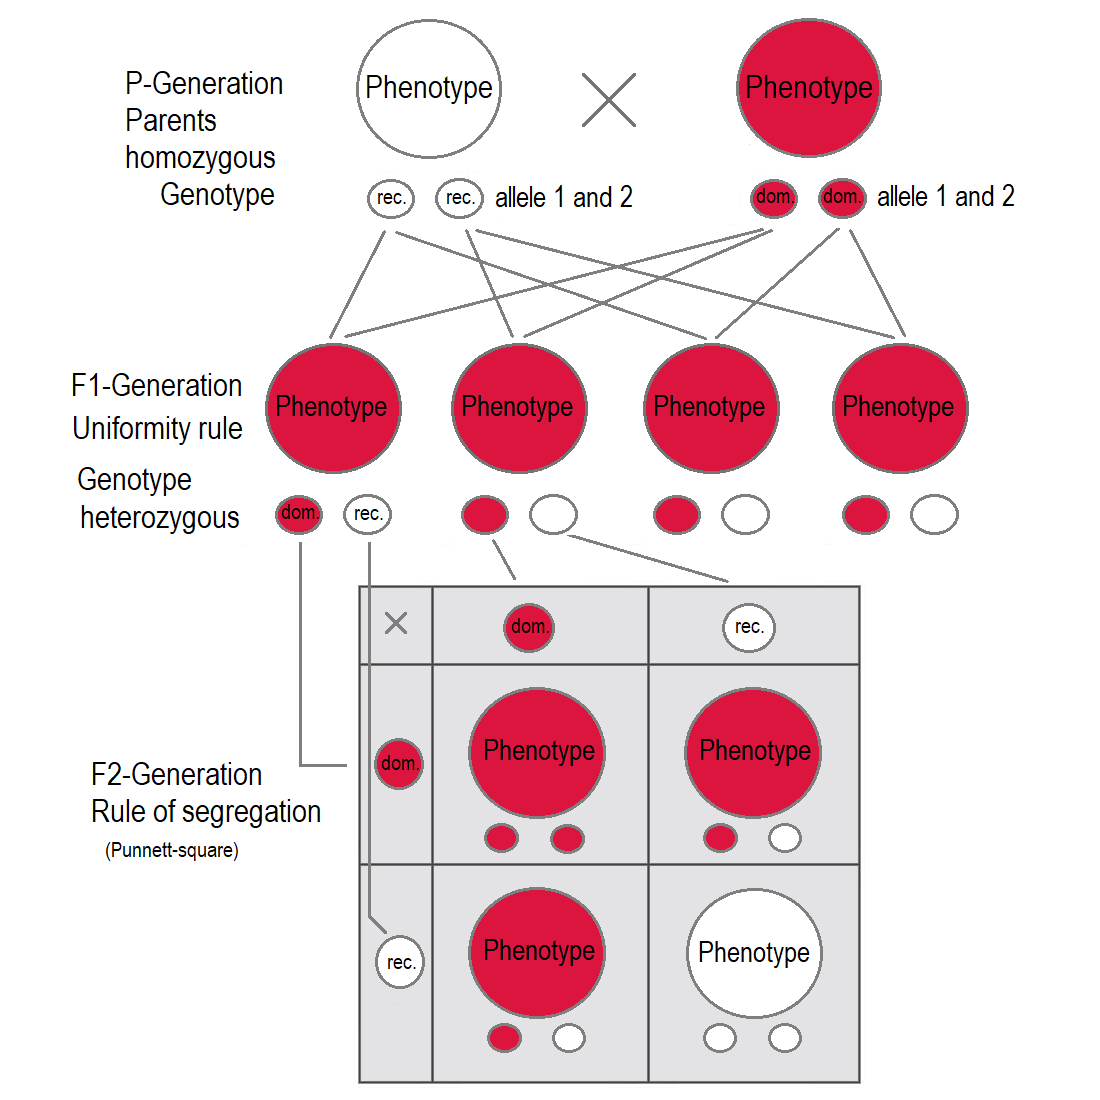
\includegraphics[width=0.7\linewidth]{./figures/mendel/Dominant-recessive_inheritance_P_-_F1_-_F2} 

}

\caption{\href{https://commons.wikimedia.org/wiki/File:Dominant-recessive_inheritance_P_-_F1_-_F2.png}{In the F1 generation all individuals have the same genotype and same phenotype expressing the dominant trait (red). In the F2 generation, the phenotypes show a 3:1 ratio. In the genotype 25\% are homozygous with the dominant trait, 50\% are heterozygous genetic carriers of the recessive trait, 25\% are homozygous with the recessive genetic trait and expressing the recessive character.}}\label{fig:dominantinheritance}
\end{figure}

But for some characteristics, the F1 hybrids have an appearance in between the phenotypes of the two parental varieties. A cross between two four o'clock (\emph{Mirabilis jalapa}) plants shows an exception to Mendel's principle, called incomplete dominance. Flowers of heterozygous plants have less pigment than the homozygous, therefore there is a third phenotype. The phenotype lies somewhere between the two homozygous genotype. In cases of intermediate inheritance (incomplete dominance) in the F1-generation Mendel's principle of uniformity in genotype and phenotype applies as well. Research about intermediate inheritance was done by other scientists. The first was Carl Correns with his studies about *Mirabilis jalapa.



\begin{figure}

{\centering 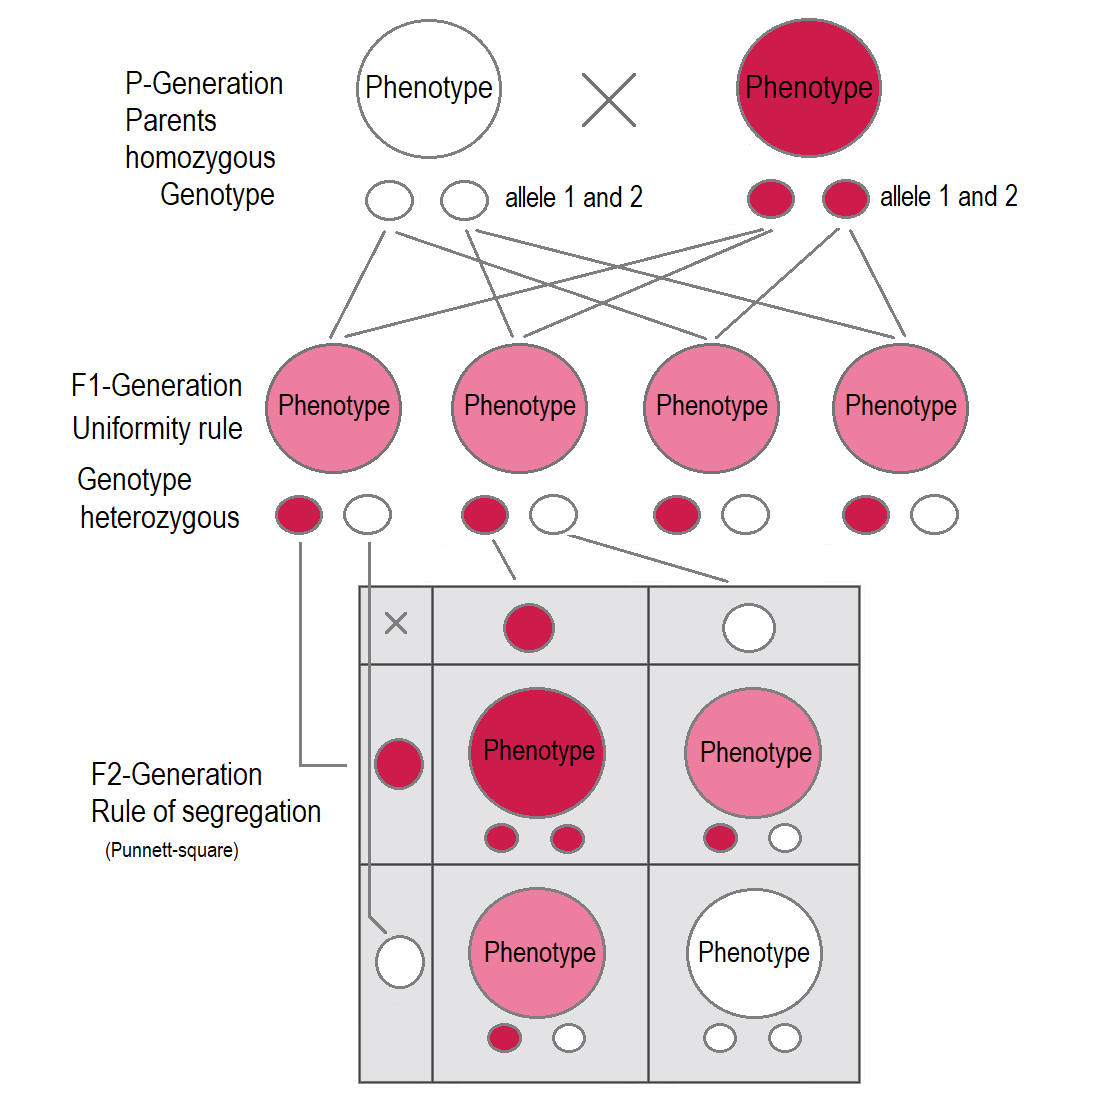
\includegraphics[width=0.7\linewidth]{./figures/mendel/Intermediate_inheritance_P_-_F1_-_F2} 

}

\caption{\href{https://commons.wikimedia.org/wiki/File:Intermediate_inheritance_P_-_F1_-_F2.png}{In \emph{Mirabilis jalapa} and \emph{Antirrhinum majus} are examples for intermediate inheritance. As seen in the F1-generation, heterozygous plants have ``light pink'' flowers---a mix of ``red'' and ``white''. The F2-generation shows a 1:2:1 ratio of red : light pink : white}}\label{fig:intermediateinheritance}
\end{figure}

\hypertarget{law-of-segregation-of-genes}{%
\section{Law of Segregation of genes}\label{law-of-segregation-of-genes}}

The Law of Segregation of genes applies when two individuals, both heterozygous for a certain trait are crossed, for example hybrids of the F1-generation. The offspring in the F2-generation differ in genotype and phenotype, so that the characteristics of the grandparents (P-generation) regularly occur again. In a dominant-recessive inheritance an average of 25\% are homozygous with the dominant trait, 50\% are heterozygous showing the dominant trait in the phenotype (genetic carriers), 25\% are homozygous with the recessive trait and therefore express the recessive trait in the phenotype. The genotypic ratio is 1 : 2 : 1, the phenotypic ratio is 3 : 1.

In the pea plant example, the capital ``B'' represents the dominant allele for purple blossom and lowercase ``b'' represents the recessive allele for white blossom. The pistil plant and the pollen plant are both F1-hybrids with genotype ``B b''. Each has one allele for purple and one allele for white. In the offspring, in the F2-plants in the Punnett-square, three combinations are possible. The genotypic ratio is 1 BB : 2 Bb : 1 bb. But the phenotypic ratio of plants with purple blossoms to those with white blossoms is 3 : 1 due to the dominance of the allele for purple. Plants with homozygous ``b b'' are white flowered like one of the grandparents in the P-generation.

In cases of incomplete dominance the same segregation of alleles takes place in the F2-generation, but here also the phenotypes show a ratio of 1 : 2 : 1, as the heterozygous are different in phenotype from the homozygous because the genetic expression of one allele compensates the missing expression of the other allele only partially. This results in an intermediate inheritance which was later described by other scientists.

In some literature sources the principle of segregation is cited as ``first law''. Nevertheless, Mendel did his crossing experiments with heterozygous plants after obtaining these hybrids by crossing two purebred plants, discovering the principle of dominance and uniformity at first.

Molecular proof of segregation of genes was subsequently found through observation of meiosis by two scientists independently, the German botanist Oscar Hertwig in 1876, and the Belgian zoologist Edouard Van Beneden in 1883. Most alleles are located in chromosomes in the cell nucleus. Paternal and maternal chromosomes get separated in meiosis, because during spermatogenesis the chromosomes are segregated on the four sperm cells that arise from one mother sperm cell, and during oogenesis the chromosomes are distributed between the polar bodys and the egg cell. Every individual organism contains two alleles for each trait. They segregate (separate) during meiosis such that each gamete contains only one of the alleles. When the gametes unite in the zygote the alleles - one from the mother one from the father - get passed on to the offspring. An offspring thus receives a pair of alleles for a trait by inheriting homologous chromosomes from the parent organisms: one allele for each trait from each parent. Heterozygous individuals with the dominant trait in the phenotype are genetic carriers of the recessive trait.

\hypertarget{law-of-independent-assortment}{%
\section{Law of Independent Assortment}\label{law-of-independent-assortment}}

The Law of Independent Assortment states that alleles for separate traits are passed independently of one another. That is, the biological selection of an allele for one trait has nothing to do with the selection of an allele for any other trait. Mendel found support for this law in his dihybrid cross experiments. In his monohybrid crosses, an idealized 3:1 ratio between dominant and recessive phenotypes resulted. In dihybrid crosses, however, he found a 9:3:3:1 ratios. This shows that each of the two alleles is inherited independently from the other, with a 3:1 phenotypic ratio for each.



\begin{figure}

{\centering 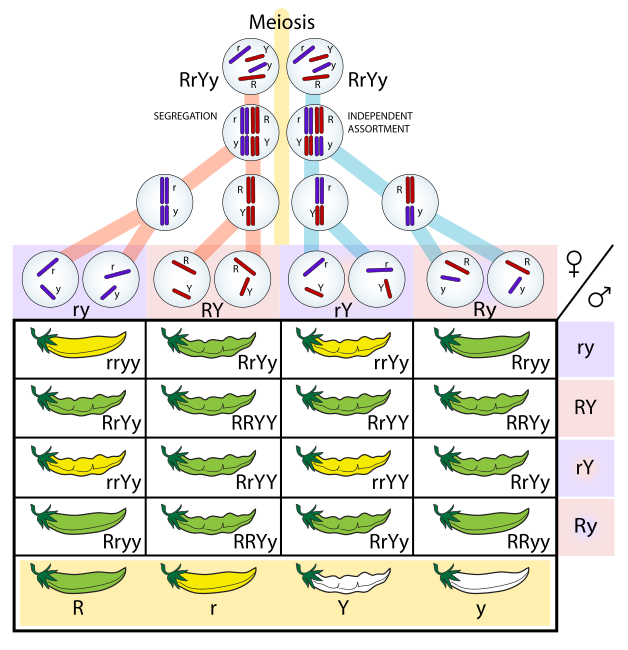
\includegraphics[width=0.7\linewidth]{./figures/mendel/Independent_assortment_&_segregation} 

}

\caption{\href{https://commons.wikimedia.org/wiki/File:Independent_assortment_\%26_segregation.svg}{Segregation and independent assortment are consistent with the chromosome theory of inheritance.}}\label{fig:assortment}
\end{figure}

Independent assortment occurs in eukaryotic organisms durig meiotic metaphase I, and produces a gamete with a mixture of the organism's chromosomes. The physical basis of the independent assortment of chromosomes is the random orientation of each bivalent chromosome along the metaphase plate with respect to the other bivalent chromosomes. Along with crossing over, independent assortment increases genetic diversity by producing novel genetic combinations.

There are many deviations from the principle of independent assortment due to genetic linkage.

Of the 46 chromosomes in a normal diploid human cell, half are maternally derived (from the mother's egg) and half are paternally derived (from the father's sperm). This occurs as sexual reproduction involves the fusion of two haploid gametes (the egg and sperm) to produce a zygote and a new organism, in which every cell has two sets of chromosomes (diploid). During gametogenesis the normal complement of 46 chromosomes needs to be halved to 23 to ensure that the resulting haploid gamete can join with another haploid gamete to produce a diploid organism.

In independent assortment, the chromosomes that result are randomly sorted from all possible maternal and paternal chromosomes. Because zygotes end up with a mix instead of a pre-defined ``set'' from either parent, chromosomes are therefore considered assorted independently. As such, the zygote can end up with any combination of paternal or maternal chromosomes. For human gametes, with 23 chromosomes, the number of possibilities is 2\textsuperscript{23} or 8,388,608 possible combinations. This contributes to the genetic variability of progeny. Generally the recombination of genes has important implications for many evolutionary processes.

\hypertarget{mendelian-trait}{%
\section{Mendelian trait}\label{mendelian-trait}}

A Mendelian trait is one that is controlled by a single locus in an inheritance pattern. In such cases, a mutation in a single gene can cause a disease that is inherited according to Mendel's principles. Dominant diseases manifest in heterozygous individuals. Recessive ones are sometimes inherited unnoticeably by genetic carriers. Examples include sickle-cell anemia, Tay--Sachs disease, cystic fibrosis and xeroderma pigmentosa. A disease controlled by a single gene contrasts with a multi-factorial disease, like heart disease, which is affected by several loci (and the environment) as well as those diseases inherited in a non-Mendelian fashion.

\hypertarget{zygosity}{%
\section{Zygosity}\label{zygosity}}

Zygosity refers to the grade of similarity between the alleles that determine one specific trait in an organism. In its simplest form, a pair of alleles can be either homozygous or heterozygous. Homozygosity, with homo relating to same while zygous pertains to a zygote, is seen when a combination of either two dominant or two recessive alleles code for the same trait. For example, using `A' as the representative character for each allele, a homozygous dominant pair's genotype would be depicted as `AA', while homozygous recessive is shown as `aa'. Heterozygosity, with hetero associated with different, can only be `Aa' (the capital letter is always presented first by convention). The phenotype of a homozygous dominant pair is `A', or dominant, while the opposite is true for homozygous recessive. Heterozygous pairs always have a dominant phenotype. To a lesser degree, hemizygosity and nullizygosity can also be seen in gene pairs.

\hypertarget{monohybrid-cross}{%
\section{Monohybrid cross}\label{monohybrid-cross}}

``Mono'' means ``one''; this cross indicates that the examination of a single trait. For example, when a strain of corn producing pure purple kernels (RR) is crossed with a strain producing pure yellow kernels (rr). In this cross, both parents are homozygous, one carrying two copies of the dominant allele (R; purple), the other two copies of the recessive (r; yellow) allele.

\hypertarget{punnett-square}{%
\section{Punnett square}\label{punnett-square}}

The \href{https://en.wikipedia.org/wiki/Punnett_square}{Punnett square} (Figures \ref{fig:punnett} and \ref{fig:punnettF1}) is a visual representation of Mendelian inheritance and used to predict an outcome of a particular cross or breeding experiment. It is named after \href{https://en.wikipedia.org/wiki/Reginald_Punnett}{Reginald C. Punnett}, who devised the approach. The diagram is used by biologists to determine the probability of an offspring having a particular genotype. The Punnett square is a tabular summary of possible combinations of maternal alleles with paternal alleles. These tables can be used to examine the genotypical outcome probabilities of the offspring of a single trait (allele), or when crossing multiple traits from the parents.

Figure \ref{fig:punnett} shows a Punnett square for a monohybrid cross. A strain of corn producing pure purple kernels (RR) is crossed with a strain producing pure yellow kernels (rr). In this cross, both parents are homozygous, one carrying two copies of the dominant allele (R; purple), the other two copies of the recessive (r; yellow) allele. Each parent can only make gametes that have either the R or r allele. The squares containing the single letters represent the possible gametes. The squares with two letters represent the zygotes resulting from the combination of the respective gametes. It can be easily seen that all offspring will be heterozygous (Rr) and therefore purple. Purple is dominant with the resulting F1 ears all bearing purple kernels. These plants that are heterozygous for a single trait are called monohybrids. When the F1 is self-pollinated, the resulting F2 ears bear both purple and yellow kernels (Figure \ref{fig:monohybrid}). The Punnett square for the F1 cross is depicted in Figure \ref{fig:punnettF1}

\begin{figure}

{\centering 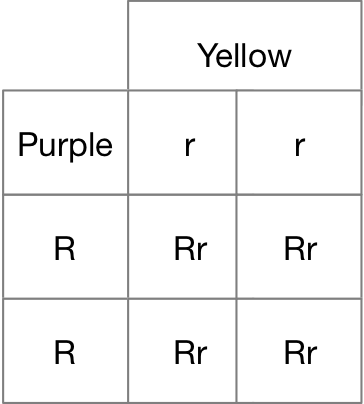
\includegraphics[width=0.7\linewidth]{./figures/mendel/Punnett} 

}

\caption{Punnett square for homozygous cross.}\label{fig:punnett}
\end{figure}

\begin{figure}

{\centering 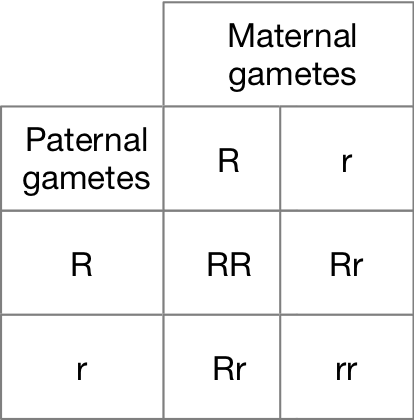
\includegraphics[width=0.7\linewidth]{./figures/mendel/PunnettF1} 

}

\caption{Punnett square for heterozygous cross.}\label{fig:punnettF1}
\end{figure}

\begin{figure}

{\centering 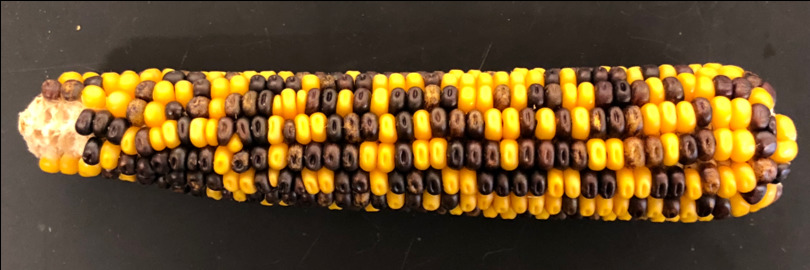
\includegraphics[width=0.7\linewidth]{./figures/mendel/Monohybrid_cross} 

}

\caption{Monohybrid cross}\label{fig:monohybrid}
\end{figure}

\hypertarget{dihybrid-cross}{%
\section{Dihybrid cross}\label{dihybrid-cross}}

More complicated crosses can be made by looking at two or more genes. The Punnett square works, however, only if the genes are independent of each other, which means that having a particular allele of gene ``A'' does not alter the probability of possessing an allele of gene ``B''. This is equivalent to stating that the genes are not linked, so that the two genes do not tend to sort together during meiosis.

A dihybrid cross is a cross between two different lines (varieties, strains) that differ in two observed traits. In the name ``Dihybrid cross'', the ``di'' indicates that there are two traits involved (in our example designated R and Su), the ``hybrid'' means that each trait has two different alleles (in our example R and r, or Su and su), and ``cross'' means that there are two individuals who are combining or ``crossing'' their genetic information. In our example, a pure strain of corn producing purple-starchy kernels (RR SuSu) is crossed with a pure strain producing yellow-sweet (rr susu). The starchy seeds are smooth, the sweet seeds are wrinkled. The resulting F1 ears all bear purple-starchy (smooth) kernels. Plants that are heterozygous for two traits are called dihybrids. When the F1 is self-pollinated, the resulting F2 generation contains various combinations (Figure \ref{fig:dihybrid}).

\begin{figure}

{\centering 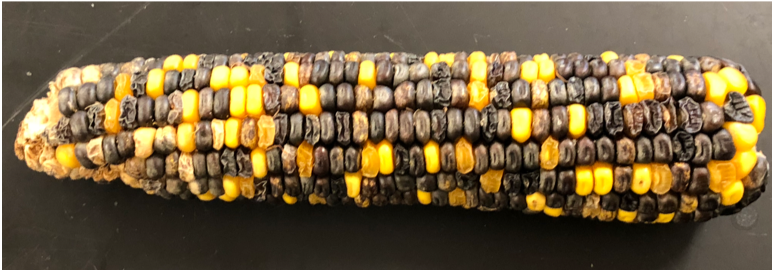
\includegraphics[width=0.7\linewidth]{./figures/mendel/Dihybrid_cross} 

}

\caption{Dihybrid cross}\label{fig:dihybrid}
\end{figure}

The rules of meiosis, as they apply to the dihybrid, are codified in Mendel's first law and Mendel's second law, which are also called the Law of Segregation and the Law of Independent Assortment, respectively (Table \ref{tab:mendel}). For genes on separate chromosomes, each allele pair showed independent segregation. If the first filial generation (F1 generation) produces four identical offspring, the second filial generation, which occurs by crossing the members of the first filial generation, shows a phenotypic (appearance) ratio of \textbf{9:3:3:1}, where:

\begin{itemize}
\tightlist
\item
  the \textbf{9} represents the proportion of individuals displaying both dominant traits
\item
  the first \textbf{3} represents the individuals displaying the first dominant trait and the second recessive trait
\item
  the second \textbf{3} represents those displaying the first recessive trait and second dominant trait
\item
  the \textbf{1} represents the homozygous, displaying both recessive traits.
\end{itemize}

\hypertarget{forked-line-method}{%
\section{Forked-line method}\label{forked-line-method}}

The forked-line method (also known as the tree method and the branching system) can also solve dihybrid and multihybrid crosses. A problem is converted to a series of monohybrid crosses, and the results are combined in a tree. However, a tree produces the same result as a Punnett square in less time and with more clarity. The example below (Figure \ref{fig:forkedline}) assesses another double-heterozygote cross using RrYy x RrYy. As stated above, the phenotypic ratio is expected to be 9:3:3:1 if crossing unlinked genes from two double-heterozygotes. The genotypic ratio was obtained in the diagram below, this diagram will have more branches than if only analyzing for phenotypic ratio.



\begin{figure}

{\centering 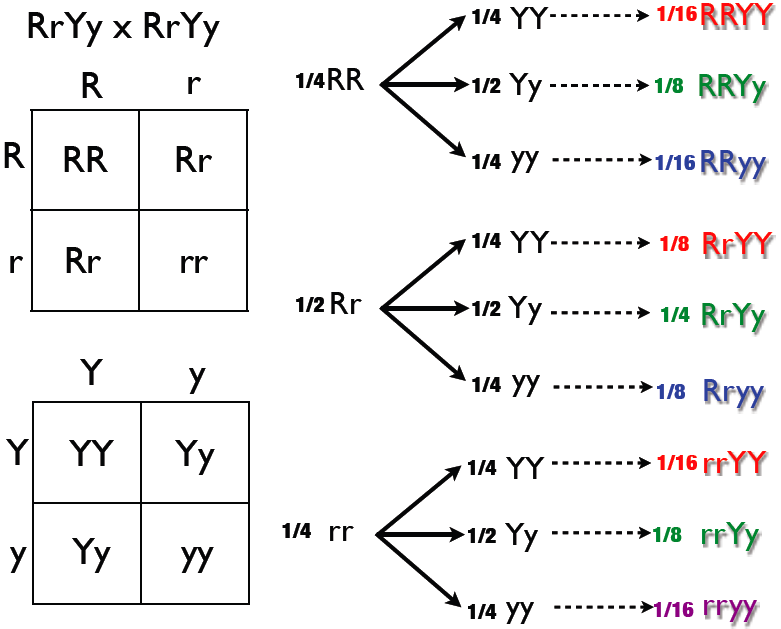
\includegraphics[width=0.7\linewidth]{./figures/mendel/Dihybrid_Cross_Tree_Method} 

}

\caption{\href{https://commons.wikimedia.org/wiki/File:Dihybrid_Cross_Tree_Method.png}{The major structures in DNA compaction: DNA, the nucleosome, the 10 nm ``beads-on-a-string'' fibre, the 30 nm fibre and the metaphase chromosome.}}\label{fig:forkedline}
\end{figure}

\hypertarget{mendelian-traits-in-humans}{%
\section{Mendelian traits in humans}\label{mendelian-traits-in-humans}}

Mendelian traits in humans concerns how, in Mendelian inheritance, a child receiving a dominant allele from either parent will have the dominant form of the phenotypic trait or characteristic. Only those that received the recessive allele from both parents, known as zygosity, will have the recessive phenotype. Those that receive a dominant allele from one parent and a recessive allele from the other parent will have the dominant form of the trait. Purely Mendelian traits are a tiny minority of all traits, since most phenotypic traits exhibit incomplete dominance, codominance, and contributions from many genes.

The recessive phenotype may theoretically skip any number of generations, lying dormant in heterozygous ``carrier'' individuals until they have children with someone who also has the recessive allele and both pass it on to their child.

Genes that do not follow Mendelian genetics include the human Y chromosome which is passed virtually unchanged from father to son. Similarly, the mitochondrial DNA (mtDNA) comes only from the mother and is given to both male and female children. Epigenetic modifications, linked genes, and duplicated genes elsewhere in the genome will also lead to a non-mendelian inheritance of traits.

Examples

\begin{itemize}
\tightlist
\item
  Albinism (recessive)
\item
  Achondroplasia
\item
  Alkaptonuria
\item
  Ataxia telangiectasia
\item
  Brachydactyly (shortness of fingers and toes)
\item
  Colour blindness (monochromatism, dichromatism, anomalous trichromatism, tritanopia, deuteranopia, protanopia)
\item
  Cystic fibrosis
\item
  Duchenne muscular dystrophy
\item
  Ectrodactyly
\item
  Ehlers--Danlos syndrome
\item
  Fabry disease
\item
  Galactosemia
\item
  Gaucher's disease
\item
  Haemophilia
\item
  Hereditary breast--ovarian cancer syndrome
\item
  Hereditary nonpolyposis colorectal cancer
\item
  HFE hereditary haemochromatosis
\item
  Huntington's disease
\item
  Hypercholesterolemia
\item
  Krabbe disease
\item
  Lactase persistence (dominant)
\item
  Leber's hereditary optic neuropathy
\item
  Lesch--Nyhan syndrome
\item
  Marfan syndrome
\item
  Niemann--Pick disease
\item
  Phenylketonuria
\item
  Porphyria
\item
  Retinoblastoma
\item
  Sickle-cell disease
\item
  Sanfilippo syndrome
\item
  Tay--Sachs disease
\item
  Wet (dominant) or dry (recessive) earwax -- dry is found mostly in Asians and Native Americans
\end{itemize}

\hypertarget{omim---online-mendelian-inheritance-in-man}{%
\section{OMIM - Online Mendelian Inheritance in Man}\label{omim---online-mendelian-inheritance-in-man}}

\href{https://omim.org}{OMIM} is a comprehensive, authoritative compendium of human genes and genetic phenotypes that is freely available and updated daily. The full-text, referenced overviews in OMIM contain information on all known mendelian disorders and over 15,000 genes. OMIM focuses on the relationship between phenotype and genotype. It is updated daily, and the entries contain copious links to other genetics resources.

The database was initiated in the early 1960s by Dr.~Victor A. McKusick as a catalog of mendelian traits and disorders, entitled Mendelian Inheritance in Man (MIM). Twelve book editions of MIM were published between 1966 and 1998. The online version, OMIM, was created in 1985 by a collaboration between the National Library of Medicine and the William H. Welch Medical Library at Johns Hopkins. It was made generally available on the internet starting in 1987. In 1995, OMIM was developed for the World Wide Web by NCBI, the National Center for Biotechnology Information.

OMIM is authored and edited at the McKusick-Nathans Institute of Genetic Medicine, Johns Hopkins University School of Medicine, under the direction of Dr.~Ada Hamosh.

\hypertarget{non-mendelian-inheritance}{%
\section{Non-Mendelian inheritance}\label{non-mendelian-inheritance}}

After Mendels studies and discoveries more and more new discoveries about genetics were made. Mendel himself has said that the regularities he discovered apply only to the organisms and characteristics he consciously chose for his experiments. Mendel explained inheritance in terms of discrete factors ---genes--- that are passed along from generation to generation according to the rules of probability. Mendel's laws are valid for all sexually reproducing organisms, including garden peas and human beings. However, Mendel's laws stop short of explaining some patterns of genetic inheritance. For most sexually reproducing organisms, cases where Mendel's laws can strictly account for all patterns of inheritance are relatively rare. Often the inheritance patterns are more complex.

In cases of codominance the phenotypes produced by both alleles are clearly expressed. Mendel chose genetic traits in plants that are determined by only two alleles, such as ``A'' and ``a''. In nature, genes often exist in several different forms with multiple alleles. Furthermore, many traits are produced by the interaction of several genes. Traits controlled by two or more genes are said to be polygenic traits.



\chapter{Chromosomes: The Vectors of Heredity}\label{chromosomes-the-vectors-of-heredity}

A \href{https://en.wikipedia.org/wiki/Chromosome}{chromosome} is a deoxyribonucleic acid (DNA) molecule with part or all of the genetic material (genome) of an organism. Most eukaryotic chromosomes include packaging proteins which, aided by chaperone proteins, bind to and condense the DNA molecule to prevent it from becoming an unmanageable tangle. This three-dimensional genome structure plays a significant role in transcriptional regulation

The word chromosome comes from the Greek χρῶμα (chroma, ``colour'') and σῶμα (soma, ``body''), describing their strong staining by particular dyes. The term was coined by the German scientist \href{https://en.wikipedia.org/wiki/Heinrich_Wilhelm_Gottfried_von_Waldeyer-Hartz}{Heinrich Wilhelm Gottfired von Waldeyer-Hartz}, referring to the term chromatin, which was itself introduced by \href{https://en.wikipedia.org/wiki/Walther_Flemming}{Walther Flemming}, who discovered cell division.

Chromosomes are normally visible under a light microscope only when the cell is undergoing cell division. Before this happens, every chromosome is copied once (S phase), and the copy is joined to the original by a centromere, resulting either in an X-shaped structure if the centromere is located in the middle of the chromosome or a two-arm structure if the centromere is located near one of the ends. The original chromosome and the copy are now called sister chromatids. During metaphase the X-shape structure is called a metaphase chromosome. In this highly condensed form chromosomes are easiest to distinguish and study. In animal cells, chromosomes reach their highest compaction level in anaphase during chromosome segregation.

Chromosomal recombination during meiosis and subsequent sexual reproduction play a significant role in genetic diversity. If these structures are manipulated incorrectly, through processes known as chromosomal instability and translocation, the cell may undergo mitotic catastrophe. Usually, this will make the cell initiate \href{https://en.wikipedia.org/wiki/Apoptosis}{apoptosis} leading to its own death, but sometimes mutations in the cell hamper this process and thus cause progression of cancer.

Some use the term chromosome in a wider sense, to refer to the individualized portions of chromatin in cells, either visible or not under light microscopy. Others use the concept in a narrower sense, to refer to the individualized portions of chromatin during cell division, visible under light microscopy due to high condensation.

The German scientists \href{https://en.wikipedia.org/wiki/Matthias_Jakob_Schleiden}{Schleiden}, \href{https://en.wikipedia.org/wiki/Rudolf_Virchow}{Virchow} and \href{https://en.wikipedia.org/wiki/Otto_Bütschli}{Bütschli} were among the first scientists who recognized the structures now familiar as chromosomes.

In a series of experiments beginning in the mid-1880s, \href{https://en.wikipedia.org/wiki/Theodor_Boveri}{Theodor Boveri} gave the definitive demonstration that chromosomes are the vectors of heredity. \href{https://en.wikipedia.org/wiki/Wilhelm_Roux}{Wilhelm Roux} suggested that each chromosome carries a different genetic configuration, and Boveri was able to test and confirm this hypothesis. Aided by the rediscovery at the start of the 1900s of Gregor Mendel's earlier work, Boveri was able to point out the connection between the rules of inheritance and the behaviour of the chromosomes.

In his famous textbook The Cell in Development and Heredity, \href{https://en.wikipedia.org/wiki/Edmund_Beecher_Wilson}{Edmund Beecher Wilson} linked together the independent work of Boveri and Sutton (both around 1902) by naming the chromosome theory of inheritance the Boveri--Sutton chromosome theory (the names are sometimes reversed). Ernst Mayr remarks that the theory was hotly contested by some famous geneticists: \href{https://en.wikipedia.org/wiki/William_Bateson}{William Bateson}, \href{https://en.wikipedia.org/wiki/Wilhelm_Johannsen}{Wilhelm Johannsen}, \href{https://en.wikipedia.org/wiki/Richard_Goldschmidt}{Richard Goldschmidt} and \href{https://en.wikipedia.org/wiki/Thomas_Hunt_Morgan}{T.H. Morgan)}. Eventually, complete proof came from chromosome maps in Morgan's own lab.

The number of human chromosomes was published in 1923 by \href{https://en.wikipedia.org/wiki/Theophilus_Painter}{Theophilus Painter}. By inspection through the microscope, he counted 24 pairs, which would mean 48 chromosomes. His error was copied by others and it was not until 1956 that the true number, 46, was determined by Indonesia-born cytogeneticist \href{https://en.wikipedia.org/wiki/Joe_Hin_Tjio}{Joe Hin Tjio}.

\hypertarget{prokaryotes}{%
\section{Prokaryotes}\label{prokaryotes}}

The prokaryotes -- bacteria and archaea -- typically have a single circular chromosome, but many variations exist. The chromosomes of most bacteria, which some authors prefer to call genophores, can range in size from only 130,000 base pairs in the endosymbiotic bacteria \emph{Candidatus Hodgkinia cicadicola} and \emph{Candidatus Tremblaya princeps}, to more than 14,000,000 base pairs in the soil-dwelling bacterium \emph{Sorangium cellulosum}. Spirochaetes of the genus Borrelia are a notable exception to this arrangement, with bacteria such as \emph{Borrelia burgdorferi}, the cause of \href{https://en.wikipedia.org/wiki/Lyme_disease}{Lyme disease}, containing a single linear chromosome.

\hypertarget{structure-in-sequences}{%
\subsection{Structure in sequences}\label{structure-in-sequences}}

Prokaryotic chromosomes have less sequence-based structure than eukaryotes. Bacteria typically have a one-point (the origin of replication) from which replication starts, whereas some archaea contain multiple replication origins. The genes in prokaryotes are often organized in \href{https://en.wikipedia.org/wiki/Operon}{operons}, and do not usually contain \href{https://en.wikipedia.org/wiki/Intron}{introns}, unlike eukaryotes.

\hypertarget{dna-packaging}{%
\subsection{DNA packaging}\label{dna-packaging}}

Prokaryotes do not possess nuclei. Instead, their DNA is organized into a structure called the nucleoid. The nucleoid is a distinct structure and occupies a defined region of the bacterial cell. This structure is, however, dynamic and is maintained and remodeled by the actions of a range of histone-like proteins, which associate with the bacterial chromosome. In archaea, the DNA in chromosomes is even more organized, with the DNA packaged within structures similar to eukaryotic nucleosomes.

Certain bacteria also contain plasmids or other extrachromosomal DNA. These are circular DNA and play a role in horizontal gene transfer.

Bacterial chromosomes tend to be tethered to the plasma membrane of the bacteria. In molecular biology application, this allows for its isolation from plasmid DNA by centrifugation of lysed bacteria and pelleting of the membranes (and the attached DNA).

Prokaryotic chromosomes and plasmids are, like eukaryotic DNA, generally supercoiled. The DNA must first be released into its relaxed state for access for transcription, regulation, and replication.

\hypertarget{eukaryotes}{%
\section{Eukaryotes}\label{eukaryotes}}

Chromosomes in eukaryotes are composed of chromatin fiber. Chromatin fiber is made of nucleosomes (histone octamers with part of a DNA strand attached to and wrapped around it). Chromatin fibers are packaged by proteins into a condensed structure called chromatin. Chromatin contains the vast majority of DNA, but a small amount inherited maternally, can be found in the mitochondria. Chromatin is present in most cells, with a few exceptions, for example, red blood cells.

Chromatin allows the very long DNA molecules to fit into the cell nucleus. During cell division chromatin condenses further to form microscopically visible chromosomes. The structure of chromosomes varies through the cell cycle. During cellular division chromosomes are replicated, divided, and passed successfully to their daughter cells so as to ensure the genetic diversity and survival of their progeny. Chromosomes may exist as either duplicated or unduplicated. Unduplicated chromosomes are single double helixes, whereas duplicated chromosomes contain two identical copies (called chromatids or sister chromatids) joined by a centromere.



\begin{figure}

{\centering 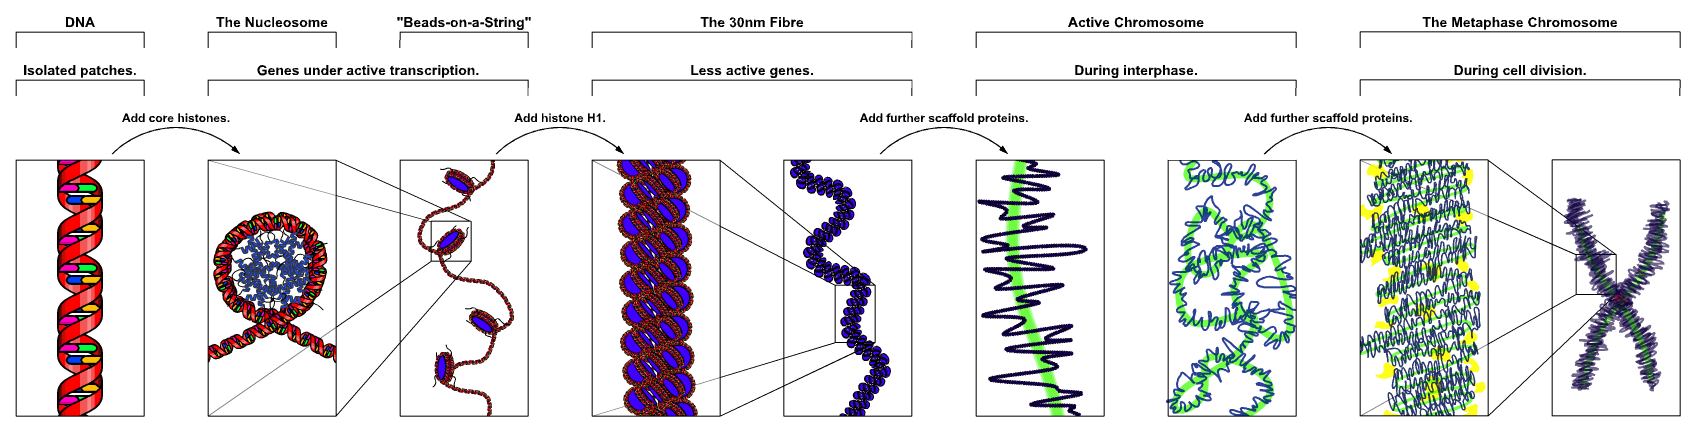
\includegraphics[width=0.7\linewidth]{./figures/chromosomes/Chromatin_Structures} 

}

\caption{\href{https://commons.wikimedia.org/wiki/File:Chromatin_Structures.png}{The major structures in DNA compaction: DNA, the nucleosome, the 10 nm ``beads-on-a-string'' fibre, the 30 nm fibre and the metaphase chromosome.}}\label{fig:structure}
\end{figure}

Eukaryotes possess multiple large linear chromosomes contained in the cell's nucleus. Each chromosome has one centromere, with one or two arms projecting from the centromere, although, under most circumstances, these arms are not visible as such. In addition, most eukaryotes have a small circular mitochondrial genome, and some eukaryotes may have additional small circular or linear cytoplasmic chromosomes.

In the nuclear chromosomes of eukaryotes, the uncondensed DNA exists in a semi-ordered structure, where it is wrapped around histones (structural proteins), forming a composite material called chromatin.

\hypertarget{interphase-chromatin}{%
\subsection{Interphase chromatin}\label{interphase-chromatin}}

During interphase (the period of the cell cycle where the cell is not dividing), two types of chromatin can be distinguished:

\begin{itemize}
\tightlist
\item
  Euchromatin, which consists of DNA that is active, e.g., being expressed as protein.
\item
  Heterochromatin, which consists of mostly inactive DNA. It seems to serve structural purposes during the chromosomal stages.
\end{itemize}

Heterochromatin can be further distinguished into two types

\begin{itemize}
\tightlist
\item
  Constitutive heterochromatin, which is never expressed. It is located around the centromere and usually contains repetitive sequences.
\item
  Facultative heterochromatin, which is sometimes expressed.
\end{itemize}

\hypertarget{metaphase-chromatin-and-division}{%
\subsection{Metaphase chromatin and division}\label{metaphase-chromatin-and-division}}

In the early stages of mitosis or meiosis (cell division), the chromatin double helix become more and more condensed. They cease to function as accessible genetic material (transcription stops) and become a compact transportable form. This compact form makes the individual chromosomes visible, and they form the classic four arm structure, a pair of sister chromatids attached to each other at the centromere. The shorter arms are called p arms (from the French petit, small) and the longer arms are called q arms (q follows p in the Latin alphabet; q-g ``grande''; alternatively it is sometimes said q is short for queue meaning tail in French). This is the only ntural context in which individual chromosomes are visible with an optical microscope.

Mitotic metaphase chromosomes are best described by a linearly organized longitudinally compressed array of consecutive chromatin loops.

During mitosis, microtubules grow from centrosomes located at opposite ends of the cell and also attach to the centromere at specialized structures called kinetochores, one of which is present on each sister chromatid. A special DNA base sequence in the region of the kinetochores provides, along with special proteins, longer-lasting attachment in this region. The microtubules then pull the chromatids apart toward the centrosomes, so that each daughter cell inherits one set of chromatids. Once the cells have divided, the chromatids are uncoiled and DNA can again be transcribed. In spite of their appearance, chromosomes are structurally highly condensed, which enables these giant DNA structures to be contained within a cell nucleus.

\hypertarget{human-chromosomes}{%
\section{Human chromosomes}\label{human-chromosomes}}

Chromosomes in humans can be divided into two types: autosomes (body chromosome(s)) and allosome (sex chromosome(s)). Certain genetic traits are linked to a person's sex and are passed on through the sex chromosomes. The autosomes contain the rest of the genetic hereditary information. All act in the same way during cell division. Human cells have 23 pairs of chromosomes (22 pairs of autosomes and one pair of sex chromosomes), giving a total of 46 per cell (Figure \ref{fig:karyotype}). In addition to these, human cells have many hundreds of copies of the mitochondrial genome. Sequencing of the human genome has provided a great deal of information about each of the chromosomes (Table \ref{tab:chr}).

\begin{longtable}[]{@{}crr@{}}
\caption{\label{tab:chr} \href{https://www.ncbi.nlm.nih.gov/grc/human/data}{Human Genome Assembly GRCh38.p12 (nucleotides) and GRCh38.p13 (coding genes)}. Length of DNA sequence and number of coding genes of each human chromosome. Total lengths are calculated by summing the length of the sequenced bases and estimated gaps.}\tabularnewline
\toprule
Chromosome & Total length & Coding genes\tabularnewline
\midrule
\endfirsthead
\toprule
Chromosome & Total length & Coding genes\tabularnewline
\midrule
\endhead
1 & 248,956,422 & 2,057\tabularnewline
2 & 242,193,529 & 1,303\tabularnewline
3 & 198,295,559 & 1,078\tabularnewline
4 & 190,214,555 & 753\tabularnewline
5 & 181,538,259 & 885\tabularnewline
6 & 170,805,979 & 1,048\tabularnewline
7 & 159,345,973 & 999\tabularnewline
8 & 145,138,636 & 685\tabularnewline
9 & 138,394,717 & 780\tabularnewline
10 & 133,797,422 & 733\tabularnewline
11 & 135,086,622 & 1,317\tabularnewline
12 & 133,275,309 & 1,034\tabularnewline
13 & 114,364,328 & 321\tabularnewline
14 & 107,043,718 & 819\tabularnewline
15 & 101,991,189 & 613\tabularnewline
16 & 90,338,345 & 859\tabularnewline
17 & 83,257,441 & 1,186\tabularnewline
18 & 80,373,285 & 268\tabularnewline
19 & 58,617,616 & 1,473\tabularnewline
20 & 64,444,167 & 546\tabularnewline
21 & 46,709,983 & 233\tabularnewline
22 & 50,818,468 & 494\tabularnewline
X & 156,040,895 & 852\tabularnewline
Y & 57,227,415 & 66\tabularnewline
MT & 16,569 & 13\tabularnewline
Unplaced & 4,485,509 &\tabularnewline
Genome & 3,099,734,149 & 20,415\tabularnewline
\bottomrule
\end{longtable}

\hypertarget{number-of-chromosomes-in-various-organisms}{%
\section{Number of chromosomes in various organisms}\label{number-of-chromosomes-in-various-organisms}}

The following tables (Tables \ref{tab:numplants} and \ref{tab:numanimals}) give the total number of chromosomes (including sex chromosomes) in a cell nucleus. For example, most eukaryotes are diploid, like humans who have 22 different types of autosomes, each present as two homologous pairs, and two sex chromosomes. This gives 46 chromosomes in total. Other organisms have more than two copies of their chromosome types, such as bread wheat, which is hexaploid and has six copies of seven different chromosome types -- 42 chromosomes in total.

Normal members of a particular eukaryotic species all have the same number of nuclear chromosomes. Other eukaryotic chromosomes, i.e., mitochondrial and plasmid-like small chromosomes, are much more variable in number, and there may be thousands of copies per cell.

\begin{longtable}[]{@{}lc@{}}
\caption{\label{tab:numplants} Chromosome numbers in some plants.}\tabularnewline
\toprule
Plant Species & \#\tabularnewline
\midrule
\endfirsthead
\toprule
Plant Species & \#\tabularnewline
\midrule
\endhead
Adder's tongue fern (polyploid) & approx. 1,200\tabularnewline
Arabidopsis thaliana (diploid) & 10\tabularnewline
Einkorn wheat (diploid) & 14\tabularnewline
Rye (diploid) & 14\tabularnewline
Maize (diploid or palaeotetraploid) & 20\tabularnewline
Durum wheat (tetraploid) & 28\tabularnewline
Bread wheat (hexaploid) & 42\tabularnewline
Cultivated tobacco (tetraploid) & 48\tabularnewline
\bottomrule
\end{longtable}

\begin{longtable}[]{@{}lc@{}}
\caption{\label{tab:numanimals} Chromosome numbers (2n) in some animals.}\tabularnewline
\toprule
Species & \#\tabularnewline
\midrule
\endfirsthead
\toprule
Species & \#\tabularnewline
\midrule
\endhead
Indian muntjac & 7\tabularnewline
Common fruit fly & 8\tabularnewline
Pill millipede (\emph{Arthrosphaera fumosa}) & 30\tabularnewline
Earthworm (\emph{Octodrilus complanatus}) & 36\tabularnewline
Tibetan fox & 36\tabularnewline
Domestic cat & 38\tabularnewline
Domestic pig & 38\tabularnewline
Laboratory mouse & 40\tabularnewline
Laboratory rat & 42\tabularnewline
Rabbit (\emph{Oryctolagus cuniculus}) & 44\tabularnewline
Syrian hamster & 44\tabularnewline
Guppy (\emph{Poecilia reticulata}) & 46\tabularnewline
Human & 46\tabularnewline
Hares & 48\tabularnewline
Gorillas, chimpanzees & 48\tabularnewline
Domestic sheep & 54\tabularnewline
Garden snail & 54\tabularnewline
Silkworm & 56\tabularnewline
Elephants & 56\tabularnewline
Cow & 60\tabularnewline
Donkey & 62\tabularnewline
Guinea pig & 64\tabularnewline
Horse & 64\tabularnewline
Dog & 78\tabularnewline
Hedgehog & 90\tabularnewline
Goldfish & 100--104\tabularnewline
Kingfisher & 132\tabularnewline
\bottomrule
\end{longtable}

Asexually reproducing species have one set of chromosomes that are the same in all body cells. However, asexual species can be either haploid or diploid.

Sexually reproducing species have somatic cells (body cells), which are diploid {[}2n{]} having two sets of chromosomes (23 pairs in humans with one set of 23 chromosomes from each parent), one set from the mother and one from the father. Gametes, reproductive cells, are haploid {[}n{]}: They have one set of chromosomes. Gametes are produced by meiosis of a diploid germ line cell. During meiosis, the matching chromosomes of father and mother can exchange small parts of themselves (crossover), and thus create new chrmosomes that are not inherited solely from either parent. When a male and a female gamete merge (fertilization), a new diploid organism is formed.

Some animal and plant species are polyploid {[}Xn{]}: They have more than two sets of homologous chromosomes. Plants important in agriculture such as tobacco or wheat are often polyploid, compared to their ancestral species. Wheat has a haploid number of seven chromosomes, still seen in some cultivars as well as the wild progenitors. The more-common pasta and bread wheat types are polyploid, having 28 (tetraploid) and 42 (hexaploid) chromosomes, compared to the 14 (diploid) chromosomes in the wild wheat.

\hypertarget{in-prokaryotes}{%
\subsection{In prokaryotes}\label{in-prokaryotes}}

Prokaryote species generally have one copy of each major chromosome, but most cells can easily survive with multiple copies. For example, Buchnera, a symbiont of aphids has multiple copies of its chromosome, ranging from 10--400 copies per cell. However, in some large bacteria, such as \emph{Epulopiscium fishelsoni} up to 100,000 copies of the chromosome can be present. Plasmids and plasmid-like small chromosomes are, as in eukaryotes, highly variable in copy number. The number of plasmids in the cell is almost entirely determined by the rate of division of the plasmid -- fast division causes high copy number.

\hypertarget{karyotype-1}{%
\section{Karyotype}\label{karyotype-1}}

In general, the karyotype is the characteristic chromosome complement of a eukaryote species. The preparation and study of karyotypes is part of cytogenetics.

Although the replication and transcription of DNA is highly standardized in eukaryotes, the same cannot be said for their karyotypes, which are often highly variable. There may be variation between species in chromosome number and in detailed organization. In some cases, there is significant variation within species. Often there is:

\begin{enumerate}
\def\labelenumi{\arabic{enumi}.}
\tightlist
\item
  variation between the two sexes
\item
  variation between the germ-line and soma (between gametes and the rest of the body)
\item
  variation between members of a population, due to balanced genetic polymorphism
\item
  geographical variation between races
\item
  mosaics or otherwise abnormal individuals.
\end{enumerate}

Also, variation in karyotype may occur during development from the fertilized egg.

The technique of determining the karyotype is usually called karyotyping. Cells can be locked part-way through division (in metaphase) in vitro (in a reaction vial) with colchicine. These cells are then stained, photographed, and arranged into a karyogram, with the set of chromosomes arranged, autosomes in order of length, and sex chromosomes (here X/Y) at the end.

Like many sexually reproducing species, humans have special gonosomes (sex chromosomes, in contrast to autosomes). These are XX in females and XY in males.

Investigation into the human karyotype (Figure \ref{fig:karyotype}) took many years to settle the most basic question: How many chromosomes does a normal diploid human cell contain? In 1912, Hans von Winiwarter reported 47 chromosomes in spermatogonia and 48 in oogonia, concluding an XX/XO sex determination mechanism. Painter in 1922 was not certain whether the diploid number of man is 46 or 48, at first favouring 46. He revised his opinion later from 46 to 48, and he correctly insisted on humans having an XX/XY system.

\href{https://commons.wikimedia.org/wiki/File:NHGRI_human_male_karyotype.png}{Human male karyotype.} \href{https://commons.wikimedia.org/wiki/File:NHGRI_human_male_karyotype.png}{Human male karyotype.}

\begin{figure}

{\centering 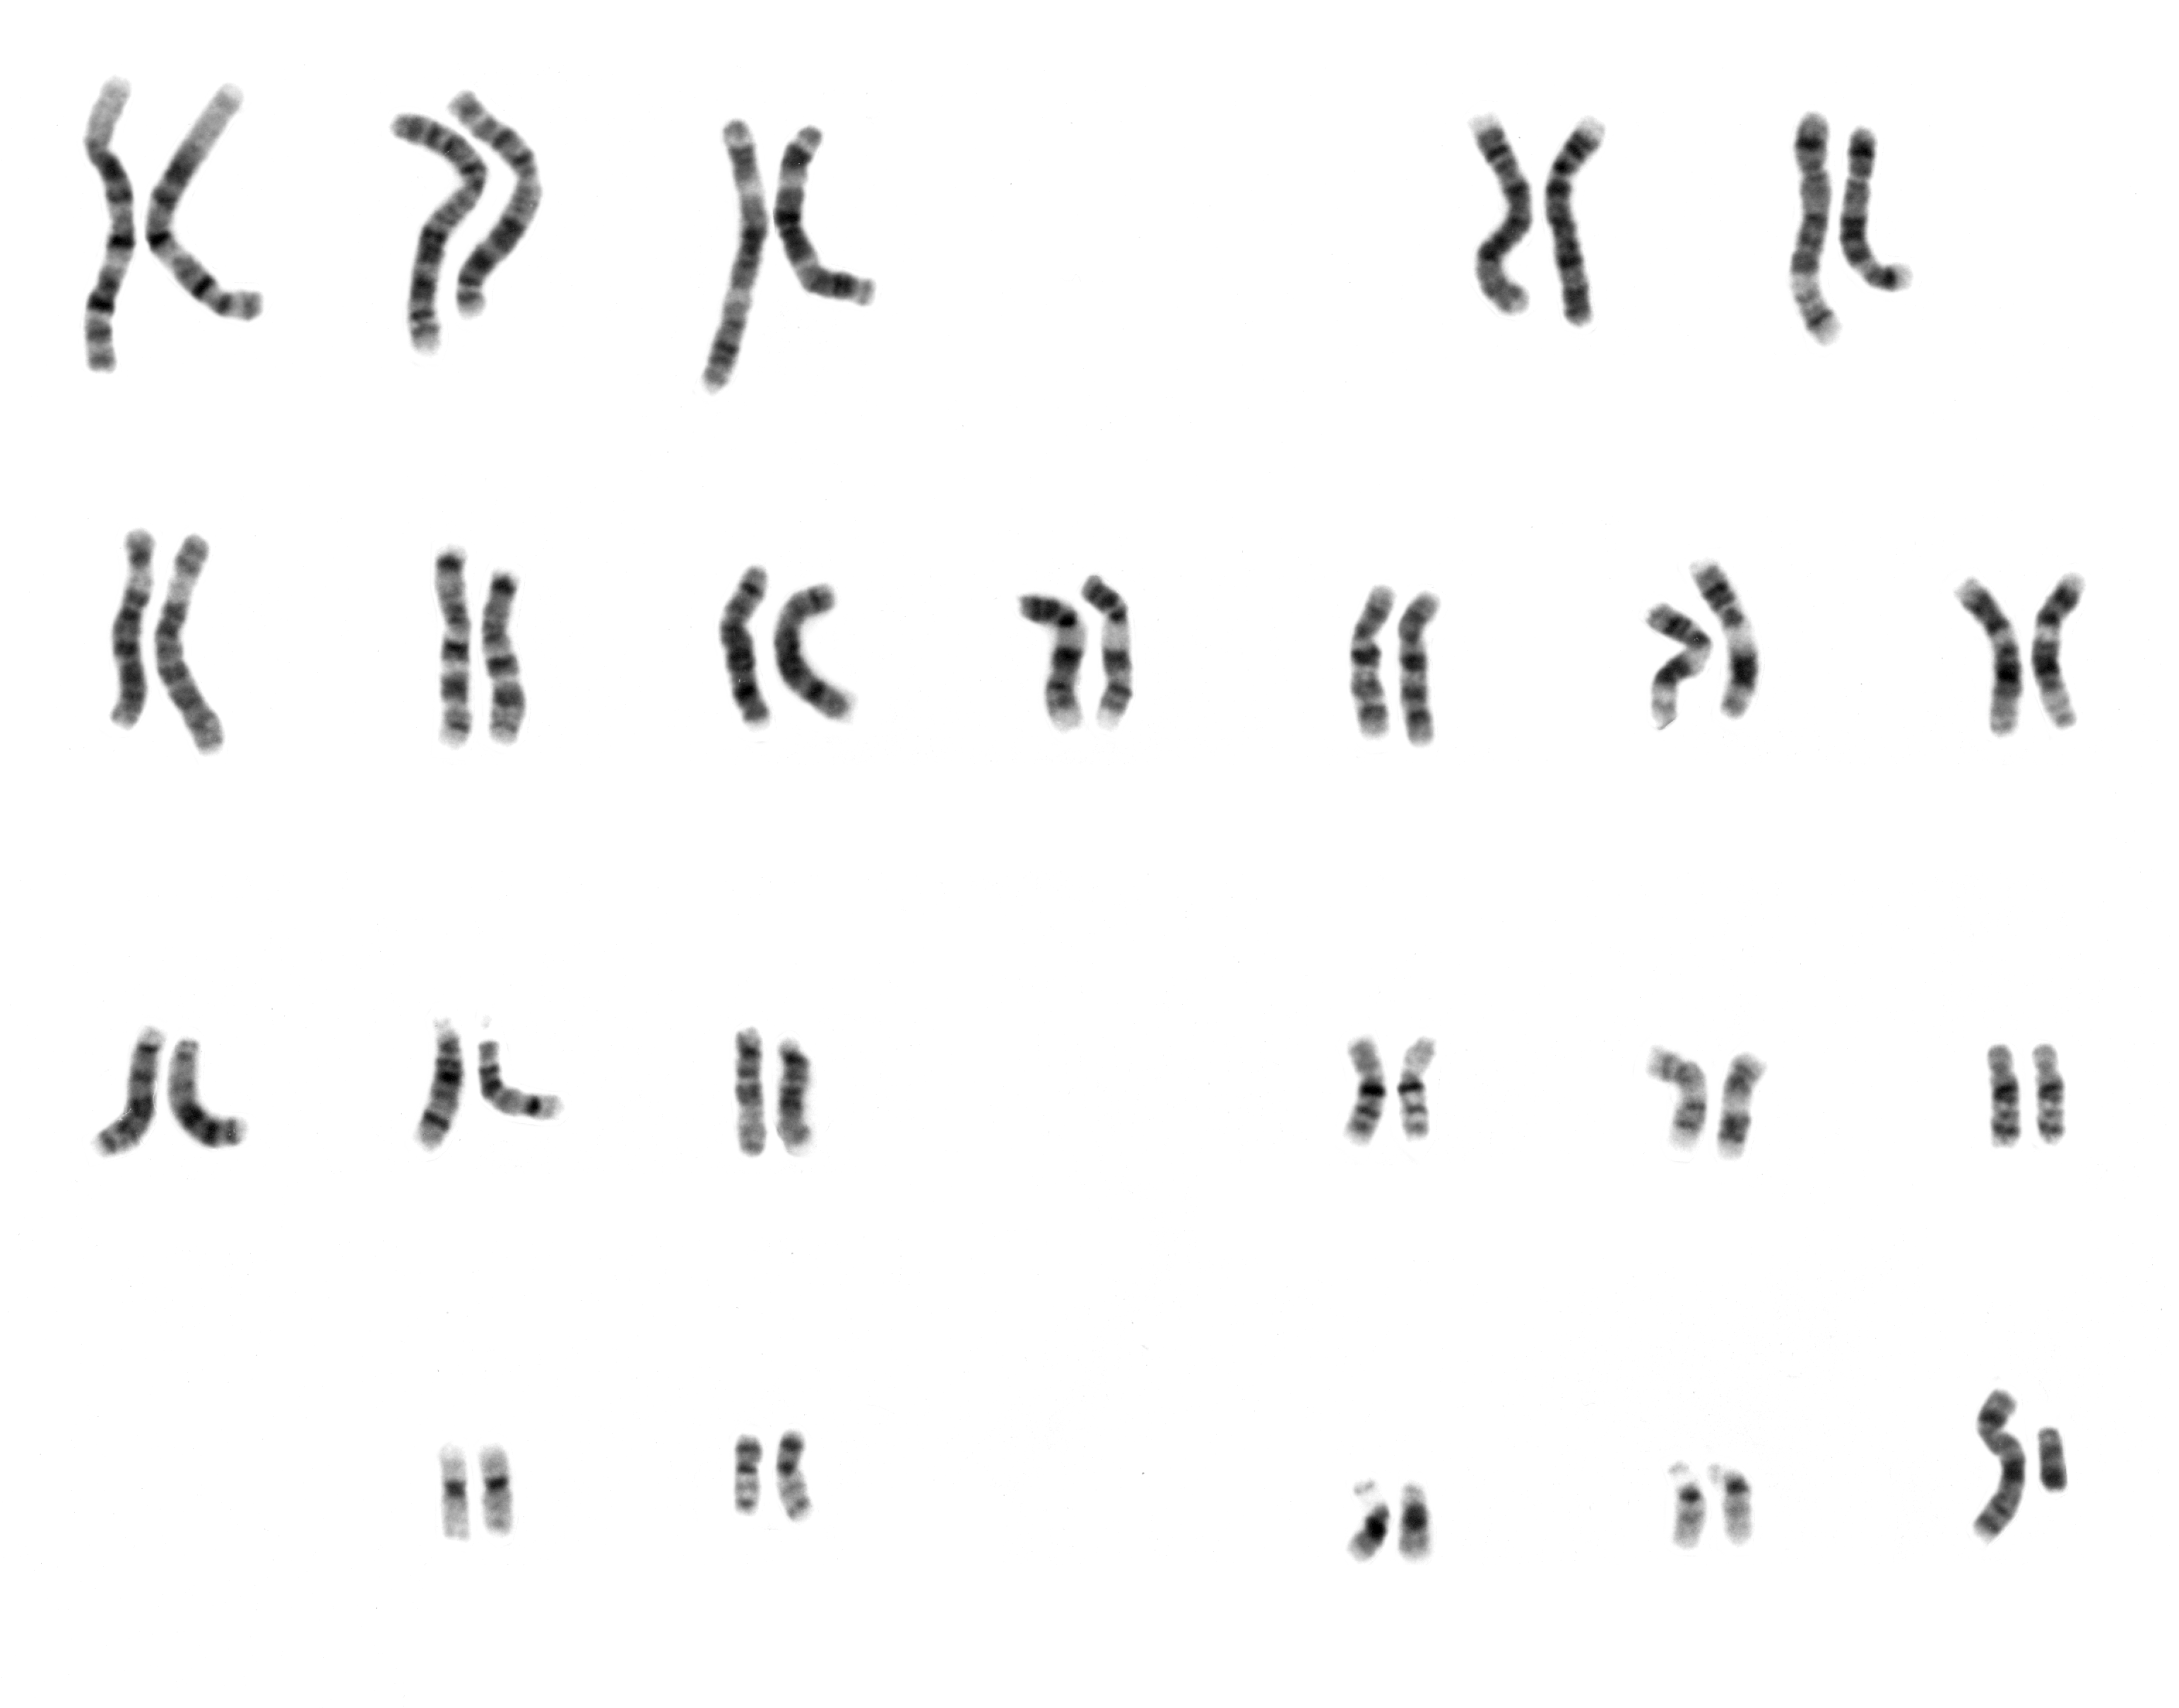
\includegraphics[width=0.7\linewidth]{./figures/chromosomes/human_male_karyotype} 

}

\caption{\href{https://commons.wikimedia.org/wiki/File:NHGRI_human_male_karyotype.png}{Human male karyotype.}}\label{fig:karyotype}
\end{figure}

New techniques were needed to definitively solve the problem:

\begin{itemize}
\tightlist
\item
  Using cells in culture
\item
  Arresting mitosis in metaphase by a solution of colchicine
\item
  Pretreating cells in a hypotonic solution 0.075 M KCl, which swells them and spreads the chromosomes
\item
  Squashing the preparation on the slide forcing the chromosomes into a single plane
\item
  Cutting up a photomicrograph and arranging the result into an indisputable karyogram.
\end{itemize}

It took until 1954 before the human diploid number was confirmed as 46. Considering the techniques of Winiwarter and Painter, their results were quite remarkable. Chimpanzees, the closest living relatives to modern humans, have 48 chromosomes as do the other great apes: in humans two chromosomes fused to form chromosome 2.



\chapter{Chromosomal Disorders}\label{chromosomal-disorders}}

A \href{https://en.wikipedia.org/wiki/Chromosome_abnormality}{chromosomal disorder}, anomaly, aberration, or mutation is a missing, extra, or irregular portion of chromosomal DNA. It can be from a typical number of chromosomes or a structural abnormality in one or more chromosomes.

\hypertarget{aberrations}{%
\section{Aberrations}\label{aberrations}}

Chromosomal aberrations are disruptions in the normal chromosomal content of a cell and are a major cause of genetic conditions in humans, such as Down syndrome, although most aberrations have little to no effect. Some chromosome abnormalities do not cause disease in carriers, such as translocations, or chromosomal inversions, although they may lead to a higher chance of bearing a child with a chromosome disorder. Abnormal numbers of chromosomes or chromosome sets, called aneuploidy, may be lethal or may give rise to genetic disorders. Genetic counseling is offered for families that may carry a chromosome rearrangement.

\hypertarget{numerical-abnormalities}{%
\section{Numerical abnormalities}\label{numerical-abnormalities}}

\href{https://en.wikipedia.org/wiki/Aneuploidy}{Aneuploidy} is the presence of an abnormal number of chromosomes in a cell, for example when an individual either is missing a chromosome from a pair (monosomy) or has more than two chromosomes of a pair (trisomy, tetrasomy, etc.). In the strict sense, a chromosome complement having a number of chromosomes other than 46 (in humans) is considered heteroploid while an exact multiple of the haploid chromosome complement is considered euploid. Thus, a cell with any number of complete chromosome sets is called a euploid cell. An extra or missing chromosome is a common cause of genetic disorders, including some human birth defects. Some cancer cells also have abnormal numbers of chromosomes. About 68\% of human solid tumors are aneuploid. Aneuploidy originates during cell division when the chromosomes do not separate properly between the two cells.

\begin{longtable}[t]{>{\raggedright\arraybackslash}p{7em}>{\raggedright\arraybackslash}p{10em}>{\raggedright\arraybackslash}p{20em}}
\caption{\label{tab:heteroploidy}Terminology and examples of heteroploidy in humans.}\\
\toprule
Number of chromosomes & Name & Description\\
\midrule
\rowcolor{gray!6}  1 & Monosomy & Monosomy refers to lack of one chromosome of the normal complement. Partial monosomy can occur in unbalanced translocations or deletions, in which only a portion of the chromosome is present in a single copy (see deletion (genetics)). Monosomy of the sex chromosomes (45,X) causes Turner syndrome.\\
2 & Disomy & Disomy is the presence of two copies of a chromosome. For organisms such as humans that have two copies of each chromosome (those that are diploid), it is the normal condition. For organisms that normally have three or more copies of each chromosome (those that are triploid or above), disomy is an aneuploid chromosome complement. In uniparental disomy, both copies of a chromosome come from the same parent (with no contribution from the other parent).\\
\rowcolor{gray!6}  3 & Trisomy & Trisomy refers to the presence of three copies, instead of the normal two, of a particular chromosome. The presence of an extra chromosome 21, which is found in Down syndrome, is called trisomy 21. Trisomy 18 and Trisomy 13, known as Edwards syndrome and Patau syndrome, respectively, are the two other autosomal trisomies recognized in live-born humans. Trisomy of the sex chromosomes is also possible, for example (47,XXX), (47,XXY), and (47,XYY).\\
4/5 & tetrasomy/pentasomy & Tetrasomy and pentasomy are the presence of four or five copies of a chromosome, respectively. Although rarely seen with autosomes, sex chromosome tetrasomy and pentasomy have been reported in humans, including XXXX, XXYY, XXXXX, XXXXY, and XYYYY.\\
\bottomrule
\end{longtable}

An example of trisomy in humans is \href{https://en.wikipedia.org/wiki/Down_syndrome}{Down syndrome}, which is a developmental disorder caused by an extra copy of chromosome 21; the disorder is therefore also called trisomy 21. Having an extra copy of this chromosome means that individuals have three copies of each of its genes instead of two, making it difficult for cells to properly control how much protein is made. Producing too much or too little protein can have serious consequences. Genes on chromosome 21 that specifically contribute to the various symptoms of Down syndrome are now being identified. The frequency of Trisomy 21 has been determined to be a function of advanced maternal age.



An example of monosomy is \href{https://en.wikipedia.org/wiki/Turner_syndrome}{Turner syndrome}, where the individual is born with only one sex chromosome, an X.

Other examples include:

\begin{itemize}
\tightlist
\item
  Cri du chat, which is caused by the deletion of part of the short arm of chromosome 5. ``Cri du chat'' means ``cry of the cat'' in French; the condition was so-named because affected babies make high-pitched cries that sound like those of a cat. Affected individuals have wide-set eyes, a small head and jaw, moderate to severe mental health problems, and are very short.
\item
  Edwards syndrome, or trisomy-18, the second most common trisomy. Symptoms include motor retardation, developmental disability and numerous congenital anomalies causing serious health problems. Ninety percent of those affected die in infancy. They have characteristic clenched hands and overlapping fingers.
\item
  Isodicentric 15, also called idic(15), partial tetrasomy 15q, or inverted duplication 15 (inv dup 15).
\item
  Jacobsen syndrome, which is very rare. It is also called the terminal 11q deletion disorder. Those affected have normal intelligence or mild developmental disability, with poor expressive language skills. Most have a bleeding disorder called Paris-Trousseau syndrome.
\item
  Klinefelter syndrome (XXY). Men with Klinefelter syndrome are usually sterile and tend to be taller and have longer arms and legs than their peers. Boys with the syndrome are often shy and quiet and have a higher incidence of speech delay and dyslexia. Without testosterone treatment, some may develop gynecomastia during puberty.
\item
  Patau Syndrome, also called D-Syndrome or trisomy-13. Symptoms are somewhat similar to those of trisomy-18, without the characteristic folded hand.
\item
  Small supernumerary marker chromosome. This means there is an extra, abnormal chromosome. Features depend on the origin of the extra genetic material. Cat-eye syndrome and isodicentric chromosome 15 syndrome (or Idic15) are both caused by a supernumerary marker chromosome, as is Pallister--Killian syndrome.
\item
  Triple-X syndrome (XXX). XXX girls tend to be tall and thin and have a higher incidence of dyslexia.
\item
  Wolf--Hirschhorn syndrome, which is caused by partial deletion of the short arm of chromosome 4. It is characterized by growth retardation, delayed motor skills development, ``Greek Helmet'' facial features, and mild to profound mental health problems.
\item
  XYY syndrome. XYY boys are usually taller than their siblings. Like XXY boys and XXX girls, they are more likely to have learning difficulties.
\end{itemize}

Chromosome abnormalities are detected in 1 of 160 live human births. Most cases of aneuploidy in the germline result in miscarriage and the most common extra autosomal chromosomes among live births are 21, 18, and 13.

Most cells in the human body have 23 pairs of chromosomes, or a total of 46 chromosomes. (The sperm and egg, or gametes, each have 23 unpaired chromosomes, and red blood cells have no nucleus and no chromosomes). One copy of each pair is inherited from the mother and the other copy is inherited from the father. The first 22 pairs of chromosomes (called autosomes) are numbered from 1 to 22, from largest to smallest. The 23rd pair of chromosomes are the sex chromosomes. Normal females have two X chromosomes, while normal males have one X chromosome and one Y chromosome. The characteristics of the chromosomes in a cell as they are seen under a light microscope are called the karyotype.

During meiosis, when germ cells divide to create sperm and egg (gametes), each half should have the same number of chromosomes. But sometimes, the whole pair of chromosomes will end up in one gamete, and the other gamete will not get that chromosome at all.

Most embryos cannot survive with a missing or extra autosome (numbered chromosome) and are spontaneously aborted. The most frequent aneuploidy in humans is trisomy 16, although fetuses affected with the full version of this chromosome abnormality do not survive to term (it is possible for surviving individuals to have the mosaic form, where trisomy 16 exists in some cells but not all). The most common aneuploidy that infants can survive with is trisomy 21, which is found in Down syndrome, affecting 1 in 800 births. Trisomy 18 (Edwards syndrome) affects 1 in 6,000 births, and trisomy 13 (Patau syndrome) affects 1 in 10,000 births. 10\% of infants with trisomy 18 or 13 reach 1 year of age.

Changes in chromosome number may not necessarily be present in all cells in an individual. When aneuploidy is detected in a fraction of cells in an individual, it is called chromosomal mosaicism. In general, individuals who are mosaic for a chromosomal aneuploidy tend to have a less severe form of the syndrome compared to those with full trisomy. For many of the autosomal trisomies, only mosaic cases survive to term. However, mitotic aneuploidy may be more common than previously recognized in somatic tissues, and aneuploidy is a characteristic of many types of tumorigenesis (see below).

\hypertarget{mechanisms}{%
\subsection{Mechanisms}\label{mechanisms}}

Nondisjunction usually occurs as the result of a weakened mitotic checkpoint, as these checkpoints tend to arrest or delay cell division until all components of the cell are ready to enter the next phase. If a checkpoint is weakened, the cell may fail to `notice' that a chromosome pair is not lined up on the mitotic plate, for example. In such a case, most chromosomes would separate normally (with one chromatid ending up in each cell), while others could fail to separate at all. This would generate a daughter cell lacking a copy and a daughter cell with an extra copy.

Completely inactive mitotic checkpoints may cause nondisjunction at multiple chromosomes, possibly all. Such a scenario could result in each daughter cell possessing a disjoint set of genetic material.

\hypertarget{diagnosis}{%
\subsection{Diagnosis}\label{diagnosis}}

Germline aneuploidy is typically detected through karyotyping, a process in which a sample of cells is fixed and stained to create the typical light and dark chromosomal banding pattern and a picture of the chromosomes is analyzed. Other techniques include fluorescence in situ hybridization (FISH), quantitative PCR of short tandem repeats, quantitative fluorescence PCR (QF-PCR), quantitative PCR dosage analysis, Quantitative Mass Spectrometry of Single Nucleotide Polymorphisms, and comparative genomic hybridization (CGH).

These tests can also be performed prenatally to detect aneuploidy in a pregnancy, through either amniocentesis or chorionic villus sampling Pregnant women of 35 years or older are offered prenatal testing because the chance of chromosomal aneuploidy increases as the mother's age increases.

Recent advances have allowed for less invasive testing methods based on the presence of fetal genetic material in maternal blood. See Triple test.

\hypertarget{structural-abnormalities}{%
\section{Structural abnormalities}\label{structural-abnormalities}}

When the chromosome's structure is altered, this can take several forms:

\begin{itemize}
\tightlist
\item
  Deletions: A portion of the chromosome is missing or deleted. Known disorders in humans include Wolf-Hirschhorn syndrome, which is caused by partial deletion of the short arm of chromosome 4; and Jacobsen syndrome, also called the terminal 11q deletion disorder.
\item
  Duplications: A portion of the chromosome is duplicated, resulting in extra genetic material. Known human disorders include Charcot-Marie-Tooth disease type 1A, which may be caused by duplication of the gene encoding peripheral myelin protein 22 (PMP22) on chromosome 17.
\item
  Translocations: A portion of one chromosome is transferred to another chromosome. There are two main types of translocations:

  \begin{itemize}
  \tightlist
  \item
    Reciprocal translocation: Segments from two different chromosomes have been exchanged.
  \item
    Robertsonian translocation: An entire chromosome has attached to another at the centromere - in humans these only occur with chromosomes 13, 14, 15, 21, and 22.
  \end{itemize}
\item
  Inversions: A portion of the chromosome has broken off, turned upside down, and reattached, therefore the genetic material is inverted.
\item
  Insertions: A portion of one chromosome has been deleted from its normal place and inserted into another chromosome.
\item
  Rings: A portion of a chromosome has broken off and formed a circle or ring. This can happen with or without loss of genetic material.
\item
  Isochromosome: Formed by the mirror image copy of a chromosome segment including the centromere.
  Chromosome instability syndromes are a group of disorders characterized by chromosomal instability and breakage. They often lead to an increased tendency to develop certain types of malignancies.
\end{itemize}

Most chromosome abnormalities occur as an accident in the egg cell or sperm, and therefore the anomaly is present in every cell of the body. Some anomalies, however, can happen after conception, resulting in Mosaicism (where some cells have the anomaly and some do not). Chromosome anomalies can be inherited from a parent or be ``de novo''. This is why chromosome studies are often performed on parents when a child is found to have an anomaly. If the parents do not possess the abnormality it was not initially inherited; however it may be transmitted to subsequent generations.

\hypertarget{acquired-chromosomal-abnormalities}{%
\section{Acquired chromosomal abnormalities}\label{acquired-chromosomal-abnormalities}}

Most cancers, if not all, could cause chromosome abnormalities, with either the formation of hybrid genes and fusion proteins, deregulation of genes and overexpression of proteins, or loss of tumor suppressor genes (see the ``Mitelman Database'' and the Atlas of Genetics and Cytogenetics in Oncology and Haematology,). Furthermore, certain consistent chromosomal abnormalities can turn normal cells into a leukemic cell such as the translocation of a gene, resulting in its inappropriate expression.

\chapter{Linkage And Gene Mapping}\label{linkage-and-gene-mapping}

\href{https://en.wikipedia.org/wiki/Genetic_linkage}{Genetic linkage} is the tendency of DNA sequences that are close together on a chromosome to be inherited together during the meiosis phase of sexual reproduction. Two genetic markers that are physically near to each other are unlikely to be separated onto different chromatids during chromosomal crossover, and are therefore said to be more linked than markers that are far apart. In other words, the nearer two genes are on a chromosome, the lower the chance of \href{https://en.wikipedia.org/wiki/Genetic_recombination}{recombination} between them, and the more likely they are to be inherited together. Markers on different chromosomes are perfectly unlinked.

\hypertarget{chromosomal-crossover}{%
\section{Chromosomal crossover}\label{chromosomal-crossover}}

\href{https://en.wikipedia.org/wiki/Chromosomal_crossover}{Chromosomal crossover}, or crossing over, is the exchange of genetic material between two homologous chromosomes non-sister chromatids that results in recombinant chromosomes during sexual reproduction. It is one of the final phases of genetic recombination, which occurs in the pachytene stage of prophase I of meiosis during a process called synapsis. Synapsis begins before the synaptonemal complex develops and is not completed until near the end of prophase I. Crossover usually occurs when matching regions on matching chromosomes break and then reconnect to the other chromosome.

Crossing over was described, in theory, by Thomas Hunt Morgan. He relied on the discovery of Frans Alfons Janssens who described the phenomenon in 1909 and had called it ``chiasmatypie''. The term chiasma is linked, if not identical, to chromosomal crossover. Morgan immediately saw the great importance of Janssens' cytological interpretation of chiasmata to the experimental results of his research on the heredity of Drosophila. The physical basis of crossing over was first demonstrated by \href{https://en.wikipedia.org/wiki/Harriet_Creighton}{Harriet Creighton} and \href{https://en.wikipedia.org/wiki/Barbara_McClintock}{Barbara McClintock} in maize (\href{https://en.wikipedia.org/wiki/Maize}{\emph{Zea mays subsp. mays}}) in 1931. She produced the first genetic map for maize, linking regions of the chromosome to physical traits. The maize genome sequence was published in 2009 in the journal \href{https://science.sciencemag.org/content/326/5956/1112}{Science}.



\begin{figure}

{\centering 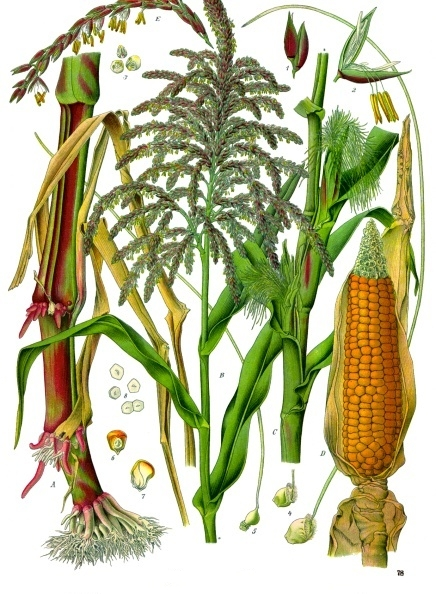
\includegraphics[width=0.7\linewidth]{./figures/linkage/Zea_mays_-_Köhler–s_Medizinal-Pflanzen-283} 

}

\caption{\href{https://commons.wikimedia.org/wiki/File:Zea_mays_-_K\%C3\%B6hler\%E2\%80\%93s_Medizinal-Pflanzen-283.jpg}{Maize: (a) Lower part of the plant (b) top of plant with male inflorescense (c) middle of plant with female inflorescenses (d) ear/cob: (1) two pollen grains of a male inflorescense (3, 4) female flowers (5) female flowers with stigma (6) fruit bottom view (7) fruit side view (8) fruit cross-section views}}\label{fig:zeamays}
\end{figure}

The linked frequency of crossing over between two gene loci (markers) is the crossing-over value . For fixed set of genetic and environmental conditions, recombination in a particular region of a linkage structure (chromosome) tends to be constant and the same is then true for the crossing-over value which is used in the production of genetic maps.

Chromosomal crossover involves recombination between the paired chromosomes inherited from each of one's parents, generally occurring during meiosis. During prophase I (pachytene stage) the four available chromatids are in tight formation with one another. While in this formation, homologous sites on two chromatids can closely pair with one another, and may exchange genetic information. The information transfer may occur without physical exchange (a section of genetic material is copied from one chromosome to another, without the donating chromosome being changed) (see SDSA pathway in Figure \ref{fig:recombination}); or by the breaking and rejoining of DNA strands, which forms new molecules of DNA (see DHJ pathway in Figure \ref{fig:recombination}).

\hypertarget{meiotic-recombination}{%
\section{Meiotic recombination}\label{meiotic-recombination}}

Meiotic recombination are initiated by double-strand breaks (DSBs) that are catalyzed by DBS-associated protein. One or more exonucleases then digest the 5' ends generated by the double-stranded breaks to produce 3' single-stranded DNA tails (see diagram). The meiosis-specific recombinase Dmc1 and the general recombinase Rad51 coat the single-stranded DNA to form nucleoprotein filaments. The recombinases catalyze invasion of the opposite chromatid by the single-stranded DNA from one end of the break. Next, the 3' end of the invading DNA primes DNA synthesis, causing displacement of the complementary strand, which subsequently anneals to the single-stranded DNA generated from the other end of the initial double-stranded break. The structure that results is a cross-strand exchange, also known as a Holliday junction. The contact between two chromatids that will soon undergo crossing-over is known as a chiasma. The Holliday junction is a tetrahedral structure which can be `pulled' by other recombinases, moving it along the four-stranded structure.



\begin{figure}

{\centering 
\includegraphics[width=0.7\linewidth]{./figures/linkage/HolidayJunction} 

}

\caption{Molecular structure of a Holliday junction (based on atomic coordinates of \href{https://www.rcsb.org/structure/3crx}{PDB 3CRX}) rendered with open source molecular visualization tool PyMol.)}\label{fig:holliday}
\end{figure}

Molecular models of meiotic recombination have evolved over the years as relevant evidence accumulated. A major incentive for developing a fundamental understanding of the mechanism of meiotic recombination is that such understanding is crucial for solving the problem of the adaptiver function of sex, a major unresolved issue in biology. A recent model that reflects current understanding was presented by Anderson and Sekelsky, and is outlined in Figure \ref{fig:recombination}). The figure shows that two of the four chromatids present early in meiosis (prophase I) are paired with each other and able to interact. Recombination, in this version of the model, is initiated by a double-strand break (or gap) shown in the DNA molecule (chromatid) at the top of the first figure in this article. However, other types of DNA damage may also initiate recombination. For instance, an inter-strand cross-link (caused by exposure to a cross-linking agent such as mitomycin C) can be repaired by HRR.



\begin{figure}

{\centering 
\includegraphics[width=0.7\linewidth]{./figures/linkage/Homologous_Recombination} 

}

\caption{\href{https://commons.wikimedia.org/wiki/File:Homologous_Recombination.jpg}{A current model of meiotic recombination, initiated by a double-strand break or gap, followed by pairing with an homologous chromosome and strand invasion to initiate the recombinational repair process. Repair of the gap can lead to crossover (CO) or non-crossover (NCO) of the flanking regions. CO recombination is thought to occur by the Double Holliday Junction (DHJ) model, illustrated on the right, above. NCO recombinants are thought to occur primarily by the Synthesis Dependent Strand Annealing (SDSA) model, illustrated on the left, above. Most recombination events appear to be the SDSA type.}}\label{fig:recombination}
\end{figure}

As shown in Figure \ref{fig:recombination}, two types of recombinant product are produced. Indicated on the right side is a ``crossover'' (CO) type, where the flanking regions of the chromosomes are exchanged, and on the left side, a ``non-crossover'' (NCO) type where the flanking regions are not exchanged. The CO type of recombination involves the intermediate formation of two ``Holliday junctions'' indicated in the lower right of the figure by two X shaped structures in each of which there is an exchange of single strands between the two participating chromatids. This pathway is labeled in the figure as the DHJ (double-Holliday junction) pathway.

The NCO recombinants (illustrated on the left in Figure \ref{fig:recombination}) are produced by a process referred to as ``synthesis dependent strand annealing'' (SDSA). Recombination events of the NCO/SDSA type appear to be more common than the CO/DHJ type.{[}citation needed{]} The NCO/SDSA pathway contributes little to genetic variation, since the arms of the chromosomes flanking the recombination event remain in the parental configuration. Thus, explanations for the adaptive function of meiosis that focus exclusively on crossing-over are inadequate to explain the majority of recombination events.
Because recombination can occur with small probability at any location along chromosome, the frequency of recombination between two locations depends on the distance separating them. Therefore, for genes sufficiently distant on the same chromosome, the amount of crossover is high enough to destroy the correlation between alleles.

Tracking the movement of genes resulting from crossovers has proven quite useful to geneticists. Because two genes that are close together are less likely to become separated than genes that are farther apart, geneticists can deduce roughly how far apart two genes are on a chromosome if they know the frequency of the crossovers. Geneticists can also use this method to infer the presence of certain genes. Genes that typically stay together during recombination are said to be linked. One gene in a linked pair can sometimes be used as a marker to deduce the presence of another gene. This is typically used in order to detect the presence of a disease-causing gene.

The recombination frequency between two loci observed is the crossing-over value. It is the frequency of crossing over between two linked gene loci (markers), and depends on the mutual distance of the genetic loci observed. For any fixed set of genetic and environmental conditions, recombination in a particular region of a linkage structure (chromosome) tends to be constant, and the same is then true for the crossing-over value which is used in the production of genetic maps.

\hypertarget{genetic-linkage}{%
\section{Genetic linkage}\label{genetic-linkage}}

Genetic linkage is the most prominent exception to Gregor Mendel's Law of Independent Assortment. The first experiment to demonstrate linkage was carried out in 1905. At the time, the reason why certain traits tend to be inherited together was unknown. Later work revealed that genes are physical structures related by physical distance.

The typical unit of genetic linkage is the centimorgan (cM). A distance of 1 cM between two markers means that the markers are separated to different chromosomes on average once per 100 meiotic product, thus once per 50 meioses

The understanding of linkage was expanded by the work of Thomas Hunt Morgan. Morgan's observation that the amount of crossing over between linked genes differs led to the idea that crossover frequency might indicate the distance separating genes on the chromosome. The centimorgan, which expresses the frequency of crossing over, is named in his honour.

A linkage map (also known as a genetic map) is a table for a species or experimental population that shows the position of its known genes or genetic markers relative to each other in terms of recombination frequency, rather than a specific physical distance along each chromosome. Linkage maps were first developed by Alfred Sturtevant, a student of Thomas Hunt Morgan.

A linkage map is a map based on the frequencies of recombination between markers during crossover of homologous chromosomes. The greater the frequency of recombination (segregation) between two genetic markers, the further apart they are assumed to be. Conversely, the lower the frequency of recombination between the markers, the smaller the physical distance between them. Historically, the markers originally used were detectable phenotypes (enzyme production, eye colour) derived from coding DNA sequences; eventually, confirmed or assumed noncoding DNA sequences such as microsatellites or those generating restriction fragment length polymorphisms (RFLPs) have been used.

Linkage maps help researchers to locate other markers, such as other genes by testing for genetic linkage of the already known markers. In the early stages of developing a linkage map, the data are used to assemble linkage groups, a set of genes which are known to be linked. As knowledge advances, more markers can be added to a group, until the group covers an entire chromosome. For well-studied organisms the linkage groups correspond one-to-one with the chromosomes.

A linkage map is not a physical map (such as a radiation reduced hybrid map) or gene map.

\hypertarget{linkage-analysis}{%
\section{Linkage analysis}\label{linkage-analysis}}

Linkage analysis is a genetic method that searches for chromosomal segments that cosegregate with the ailment phenotype through families and is the analysis technique that has been used to determine the bulk of lipodystrophy genes. It can be used to map genes for both binary and quantitative traits. Linkage analysis may be either parametric (if we know the relationship between phenotypic and genetic similarity) or non-parametric. Parametric linkage analysis is the traditional approach, whereby the probability that a gene important for a disease is linked to a genetic marker is studied through the LOD score, which assesses the probability that a given pedigree, where the disease and the marker are cosegregating, is due to the existence of linkage (with a given linkage value) or to chance. Non-parametric linkage analysis, in turn, studies the probability of an allele being identical by descent with itself.

\hypertarget{parametric-linkage-analysis}{%
\subsection{Parametric linkage analysis}\label{parametric-linkage-analysis}}

The LOD score (logarithm (base 10) of odds), developed by Newton Morton, is a statistical test often used for linkage analysis in human, animal, and plant populations. The LOD score compares the likelihood of obtaining the test data if the two loci are indeed linked, to the likelihood of observing the same data purely by chance. Positive LOD scores favour the presence of linkage, whereas negative LOD scores indicate that linkage is less likely. Computerised LOD score analysis is a simple way to analyse complex family pedigrees in order to determine the linkage between Mendelian traits (or between a trait and a marker, or two markers).

The method essentially works as follows:

\begin{itemize}
\tightlist
\item
  Establish a pedigree
\item
  Make a number of estimates of recombination frequency
\item
  Calculate a LOD score for each estimate
\end{itemize}

The estimate with the highest LOD score will be considered the best estimate.

The LOD score is calculated as follows:

\(LOD = Z = \log_{10}\frac{probability\ of\ birth\ sequence\ with\ a\ given\ linkage\ value}{probability\ of\ birth\ sequence\ with\ no\ linkage\ value} = \log_{10}\frac{1-\theta^{N\theta} \times \theta^R}{0.5^{NR+R}}\)

NR denotes the number of non-recombinant offspring, and R denotes the number of recombinant offspring. The reason 0.5 is used in the denominator is that any alleles that are completely unlinked (e.g.~alleles on separate chromosomes) have a 50\% chance of recombination, due to independent assortment. θ is the recombinant fraction, i.e.~the fraction of births in which recombination has happened between the studied genetic marker and the putative gene associated with the disease. Thus, it is equal to R / (NR + R).

By convention, a LOD score greater than 3.0 is considered evidence for linkage, as it indicates 1000 to 1 odds that the linkage being observed did not occur by chance. On the other hand, a LOD score less than −2.0 is considered evidence to exclude linkage. Although it is very unlikely that a LOD score of 3 would be obtained from a single pedigree, the mathematical properties of the test allow data from a number of pedigrees to be combined by summing their LOD scores. A LOD score of 3 translates to a p-value of approximately 0.05, and no multiple testing correction (e.g.~Bonferroni correction) is required.

Linkage analysis has a number of methodological and theoretical limitations that can significantly increase the type-1 error rate and reduce the power to map human quantitative trait loci (QTL). While linkage analysis was successfully used to identify genetic variants that contribute to rare disorders such as Huntington disease, it did not perform that well when applied to more common disorders such as heart disease or different forms of cancer. An explanation for this is that the genetic mechanisms affecting common disorders are different from those causing rare disorders.

\hypertarget{quantification-of-genetic-linkage}{%
\section{Quantification of genetic linkage}\label{quantification-of-genetic-linkage}}

Recombination frequency is a measure of genetic linkage and is used in the creation of a genetic linkage map. Recombination frequency (θ) is the frequency with which a single chromosomal crossover will take place between two genes during meiosis. A centimorgan (cM) is a unit that describes a recombination frequency of 1\%. In this way we can measure the genetic distance between two loci, based upon their recombination frequency. This is a good estimate of the real distance. Double crossovers would turn into no recombination. In this case we cannot tell if crossovers took place. If the loci we're analysing are very close (less than 7 cM) a double crossover is very unlikely. When distances become higher, the likelihood of a double crossover increases. As the likelihood of a double crossover increases we systematically underestimate the genetic distance between two loci.

During meiosis, chromosomes assort randomly into gametes, such that the segregation of alleles of one gene is independent of alleles of another gene. This is stated in Mendel's Second Law and is known as the law of independent assortment. The law of independent assortment always holds true for genes that are located on different chromosomes, but for genes that are on the same chromosome, it does not always hold true.

As an example of independent assortment, consider the crossing of the pure-bred homozygote parental strain with genotype AABB with a different pure-bred strain with genotype aabb. A and a and B and b represent the alleles of genes A and B. Crossing these homozygous parental strains will result in F1 generation offspring that are double heterozygotes with genotype AaBb. The F1 offspring AaBb produces gametes that are AB, Ab, aB, and ab with equal frequencies (25\%) because the alleles of gene A assort independently of the alleles for gene B during meiosis. Note that 2 of the 4 gametes (50\%)---Ab and aB---were not present in the parental generation. These gametes represent recombinant gametes. Recombinant gametes are those gametes that differ from both of the haploid gametes that made up the original diploid cell. In this example, the recombination frequency is 50\% since 2 of the 4 gametes were recombinant gametes.

The recombination frequency will be 50\% when two genes are located on different chromosomes or when they are widely separated on the same chromosome. This is a consequence of independent assortment.

When two genes are close together on the same chromosome, they do not assort independently and are said to be linked. Whereas genes located on different chromosomes assort independently and have a recombination frequency of 50\%, linked genes have a recombination frequency that is less than 50\%.

As an example of linkage, consider the classic experiment by William Bateson and Reginald Punnett. They were interested in trait inheritance in the sweet pea and were studying two genes---the gene for flower colour (P, purple, and p, red) and the gene affecting the shape of pollen grains (L, long, and l, round). They crossed the pure lines PPLL and ppll (the parental generation) and then self-crossed the resulting PpLl lines (the F1 generation). According to Mendelian genetics, the expected phenotypes in the F2 generation would occur in a 9:3:3:1 ratio of PL:Pl:pL:pl. To their surprise, they observed an increased frequency of PL and pl and a decreased frequency of Pl and pL (Table \ref{tab:bsp}).

\begin{longtable}[t]{>{\raggedright\arraybackslash}p{10em}>{\raggedleft\arraybackslash}p{10em}>{\raggedleft\arraybackslash}p{10em}}
\caption{\label{tab:bsp}Bateson, Saunders, and Punnett experiment}\\
\toprule
Phenotype and genotype & Observed & Expected\\
\midrule
\rowcolor{gray!6}  Purple, long (P\_L\_) & 1528 & 1199\\
Purple, round (P\_ll) & 106 & 400\\
\rowcolor{gray!6}  Red, long (ppL\_) & 117 & 400\\
Red, round (ppll) & 381 & 133\\
\rowcolor{gray!6}  Total & 2132 & 2132\\
\bottomrule
\end{longtable}

Their experiment revealed linkage between the P and L alleles and the p and l alleles. The frequency of P occurring together with L and p occurring together with l is greater than that of the recombinant Pl and pL. The recombination frequency is more difficult to compute in an F2 cross than a backcross, but the lack of fit between observed and expected numbers of progeny in the above table indicate it is less than 50\%. This indicated that two factors interacted in some way to create this difference by masking the appearance of the other two phenotypes. This led to the conclusion that some traits are related to each other because of their near proximity to each other on a chromosome. This provided the grounds to determine the difference between independent and codependent alleles.

The progeny in this case received two dominant alleles linked on one chromosome (referred to as coupling or cis arrangement). However, after crossover, some progeny could have received one parental chromosome with a dominant allele for one trait (e.g.~Purple) linked to a recessive allele for a second trait (e.g.~round) with the opposite being true for the other parental chromosome (e.g.~red and Long). This is referred to as repulsion or a trans arrangement. The phenotype here would still be purple and long but a test cross of this individual with the recessive parent would produce progeny with much greater proportion of the two crossover phenotypes. While such a problem may not seem likely from this example, unfavourable repulsion linkages do appear when breeding for disease resistance in some crops.

The two possible arrangements, cis and trans, of alleles in a double heterozygote are referred to as gametic phases, and phasing is the process of determining which of the two is present in a given individual.

When two genes are located on the same chromosome, the chance of a crossover producing recombination between the genes is related to the distance between the two genes. Thus, the use of recombination frequencies has been used to develop linkage maps or genetic maps.

However, it is important to note that recombination frequency tends to underestimate the distance between two linked genes. This is because as the two genes are located farther apart, the chance of double or even number of crossovers between them also increases. Double or even number of crossovers between the two genes results in them being cosegregated to the same gamete, yielding a parental progeny instead of the expected recombinant progeny. As mentioned above, the Kosambi and Haldane transformations attempt to correct for multiple crossovers.

While recombination of chromosomes is an essential process during meiosis, there is a large range of frequency of cross overs across organisms and within species. Sexually dimorphic rates of recombination are termed heterochiasmy, and are observed more often than a common rate between male and females. In mammals, females often have a higher rate of recombination compared to males. It is theorised that there are unique selections acting or meiotic drivers which influence the difference in rates. The difference in rates may also reflect the vastly different environments and conditions of meiosis in oogenesis and spermatogenesis.{[}citation needed{]}

With very large pedigrees or with very dense genetic marker data, such as from whole-genome sequencing, it is possible to precisely locate recombinations. With this type of genetic analysis, a meiosis indicator is assigned to each position of the genome for each meiosis in a pedigree. The indicator indicates which copy of the parental chromosome contributes to the transmitted gamete at that position. For example, if the allele from the `first' copy of the parental chromosome is transmitted, a `0' might be assigned to that meiosis. If the allele from the `second' copy of the parental chromosome is transmitted, a `1' would be assigned to that meiosis. The two alleles in the parent came, one each, from two grandparents. These indicators are then used to determine \href{https://en.wikipedia.org/wiki/Identity_by_descent}{identical-by-descent} (IBD) states or inheritance states, which are in turn used to identify genes responsible for diseases.

A DNA segment is identical by state (IBS) in two or more individuals if they have identical nucleotide sequences in this segment. An IBS segment is identical by descent (IBD) in two or more individuals if they have inherited it from a common ancestor without recombination, that is, the segment has the same ancestral origin in these individuals. DNA segments that are IBD are IBS per definition, but segments that are not IBD can still be IBS due to the same mutations in different individuals or recombinations that do not alter the segment.

All individuals in a finite population are related if traced back long enough and will, therefore, share segments of their genomes IBD. During meiosis segments of IBD are broken up by recombination. Therefore, the expected length of an IBD segment depends on the number of generations since the most recent common ancestor at the locus of the segment. The length of IBD segments that result from a common ancestor n generations in the past (therefore involving 2n meiosis) is exponentially distributed with mean 1/(2n) Morgans (M). The expected number of IBD segments decreases with the number of generations since the common ancestor at this locus. For a specific DNA segment, the probability of being IBD decreases as 2−2n since in each meiosis the probability of transmitting this segment is 1/2.

Identified IBD segments can be used for a wide range of purposes. As noted above the amount (length and number) of IBD sharing depends on the familial relationships between the tested individuals. Therefore, one application of IBD segment detection is to quantify relatedness. Measurement of relatedness can be used in forensic genetics, but can also increase information in genetic linkage mapping and help to decrease bias by undocumented relationships in standard association studies. Another application of IBD is genotype imputation and haplotype phase inference. Long shared segments of IBD, which are broken up by short regions may be indicative for phasing errors.

\hypertarget{gene-mapping}{%
\section{Gene mapping}\label{gene-mapping}}

Gene mapping describes the methods used to identify the locus of a gene and the distances between genes. The process to identify a genetic element that is responsible for a disease is also referred to as ``mapping''. If the locus in which the search is performed is already considerably constrained, the search is called the fine mapping of a gene. This information is derived from the investigation of disease manifestations in large families (genetic linkage) or from populations-based genetic association studies.

There are two distinctive types of ``maps'' used in the field of genome mapping: genetic maps and physical maps. While both maps are a collection of genetic markers and gene loci, genetic maps' distances are based on the genetic linkage information, while physical maps use actual physical distances usually measured in number of base pairs. While the physical map could be a more ``accurate'' representation of the genome, genetic maps often offer insights into the nature of different regions of the chromosome, e.g.~the genetic distance to physical distance ratio varies greatly at different genomic regions which reflects different recombination rates, and such rate is often indicative of euchromatic (usually gene-rich) vs heterochromatic (usually gene poor) regions of the genome.

\hypertarget{genetic-mapping}{%
\subsection{Genetic mapping}\label{genetic-mapping}}

Researchers begin a genetic map by collecting samples of blood., saliva, or tissue from family members that carry a prominent disease or trait and family members that don't. The most common sample used in gene mapping, especially in personal genomic tests is saliva. Scientists then isolate DNA from the samples and closely examine it, looking for unique patterns in the DNA of the family members who do carry the disease that the DNA of those who don't carry the disease don't have. These unique molecular patterns in the DNA are referred to as polymorphisms, or markers.

The first steps of building a genetic map are the development of genetic markers and a mapping population. The closer two markers are on the chromosome, the more likely they are to be passed on to the next generation together. Therefore, the ``co-segregation'' patterns of all markers can be used to reconstruct their order. With this in mind, the genotypes of each genetic marker are recorded for both parents and each individual in the following generations. The quality of the genetic maps is largely dependent upon these factors: the number of genetic markers on the map and the size of the mapping population. The two factors are interlinked, as a larger mapping population could increase the ``resolution'' of the map and prevent the map from being ``saturated''.

In gene mapping, any sequence feature that can be faithfully distinguished from the two parents can be used as a genetic marker. Genes, in this regard, are represented by ``traits'' that can be faithfully distinguished between two parents. Their linkage with other genetic markers is calculated in the same way as if they are common markers and the actual gene loci are then bracketed in a region between the two nearest neighboring markers. The entire process is then repeated by looking at more markers that target that region to map the gene neighborhood to a higher resolution until a specific causative locus can be identified. This process is often referred to as "positional cloning. The great advantage of genetic mapping is that it can identify the relative position of genes based solely on their phenotypic effect.

\hypertarget{physical-mapping}{%
\subsection{Physical mapping}\label{physical-mapping}}

Since actual base-pair distances are generally hard or impossible to directly measure, physical maps are actually constructed by first shattering the genome into hierarchically smaller pieces. By characterizing each single piece and assembling back together, the overlapping path or ``tiling path'' of these small fragments would allow researchers to infer physical distances between genomic features. The fragmentation of the genome can be achieved by restriction enzyme cutting or by physically shattering the genome by processes like sonication. Once cut, the DNA fragments are separated by electrophoresis. The resulting pattern of DNA migration (i.e.~its genetic fingerprint) is used to identify what stretch of DNA is in the clone. By analyzing the fingerprints, contigs are assembled by automated (FPC) or manual means (pathfinders) into overlapping DNA stretches. Now a good choice of clones can be made to efficiently sequence the clones to determine the DNA sequence of the organism under study.

In physical mapping, there are no direct ways of marking up a specific gene since the mapping does not include any information that concerns traits and functions. Genetic markers can be linked to a physical map by processes like in situ hybridization. By this approach, physical map contigs can be ``anchored'' onto a genetic map. The clones used in the physical map contigs can then be sequenced on a local scale to help new genetic marker design and identification of the causative loci.

Macrorestriction is a type of physical mapping wherein the high molecular weight DNA is digested with a restriction enzyme having a low number of restriction sites.

There are alternative ways to determine how DNA in a group of clones overlaps without completely sequencing the clones. Once the map is determined, the clones can be used as a resource to efficiently contain large stretches of the genome. This type of mapping is more accurate than genetic maps.

\hypertarget{genome-sequencing}{%
\subsection{Genome sequencing}\label{genome-sequencing}}

Genome sequencing is sometimes mistakenly referred to as ``genome mapping'' by non-biologists. The process of ``shotgun sequencing'' resembles the process of physical mapping: it shatters the genome into small fragments, characterizes each fragment, then puts them back together (more recent sequencing technologies are drastically different). While the scope, purpose and process are totally different, a genome assembly can be viewed as the ``ultimate'' form of physical map, in that it provides in a much better way all the information that a traditional physical map can offer.

Identification of genes is usually the first step in understanding a genome of a species; mapping of the gene is usually the first step of identification of the gene. Gene mapping is usually the starting point of many important downstream studies.



\chapter{DNA and RNA}\label{dna-and-rna}

\href{https://en.wikipedia.org/wiki/DNA}{Deoxyribonucleic acid} (DNA) is a molecule composed of two chains that coil around each other to form a double helix carrying genetic instructions for the development, functioning, growth and reproduction of all known organisms and many viruses. DNA and ribonucleic acid (RNA) are nucleic acids; alongside proteins, lipids and complex carbohydrates (polysaccharides), nucleic acids are one of the four major types of macromolecules that are essential for all known forms of life.

The structure of the DNA double helix. A section of DNA. The bases lie horizontally between the two spiraling strands (based on atomic coordinates of \href{https://www.rcsb.org/structure/1bna}{PDB 1bna} rendered with \href{https://www.cgl.ucsf.edu/chimera/}{UCSF Chimera}.) The structure of the DNA double helix. A section of DNA. The bases lie horizontally between the two spiraling strands. The atoms in the structure are colour-coded by element (based on atomic coordinates of \href{https://www.rcsb.org/structure/1bna}{PDB 1bna} rendered with open source molecular visualization tool PyMol.)

\begin{figure}

{\centering 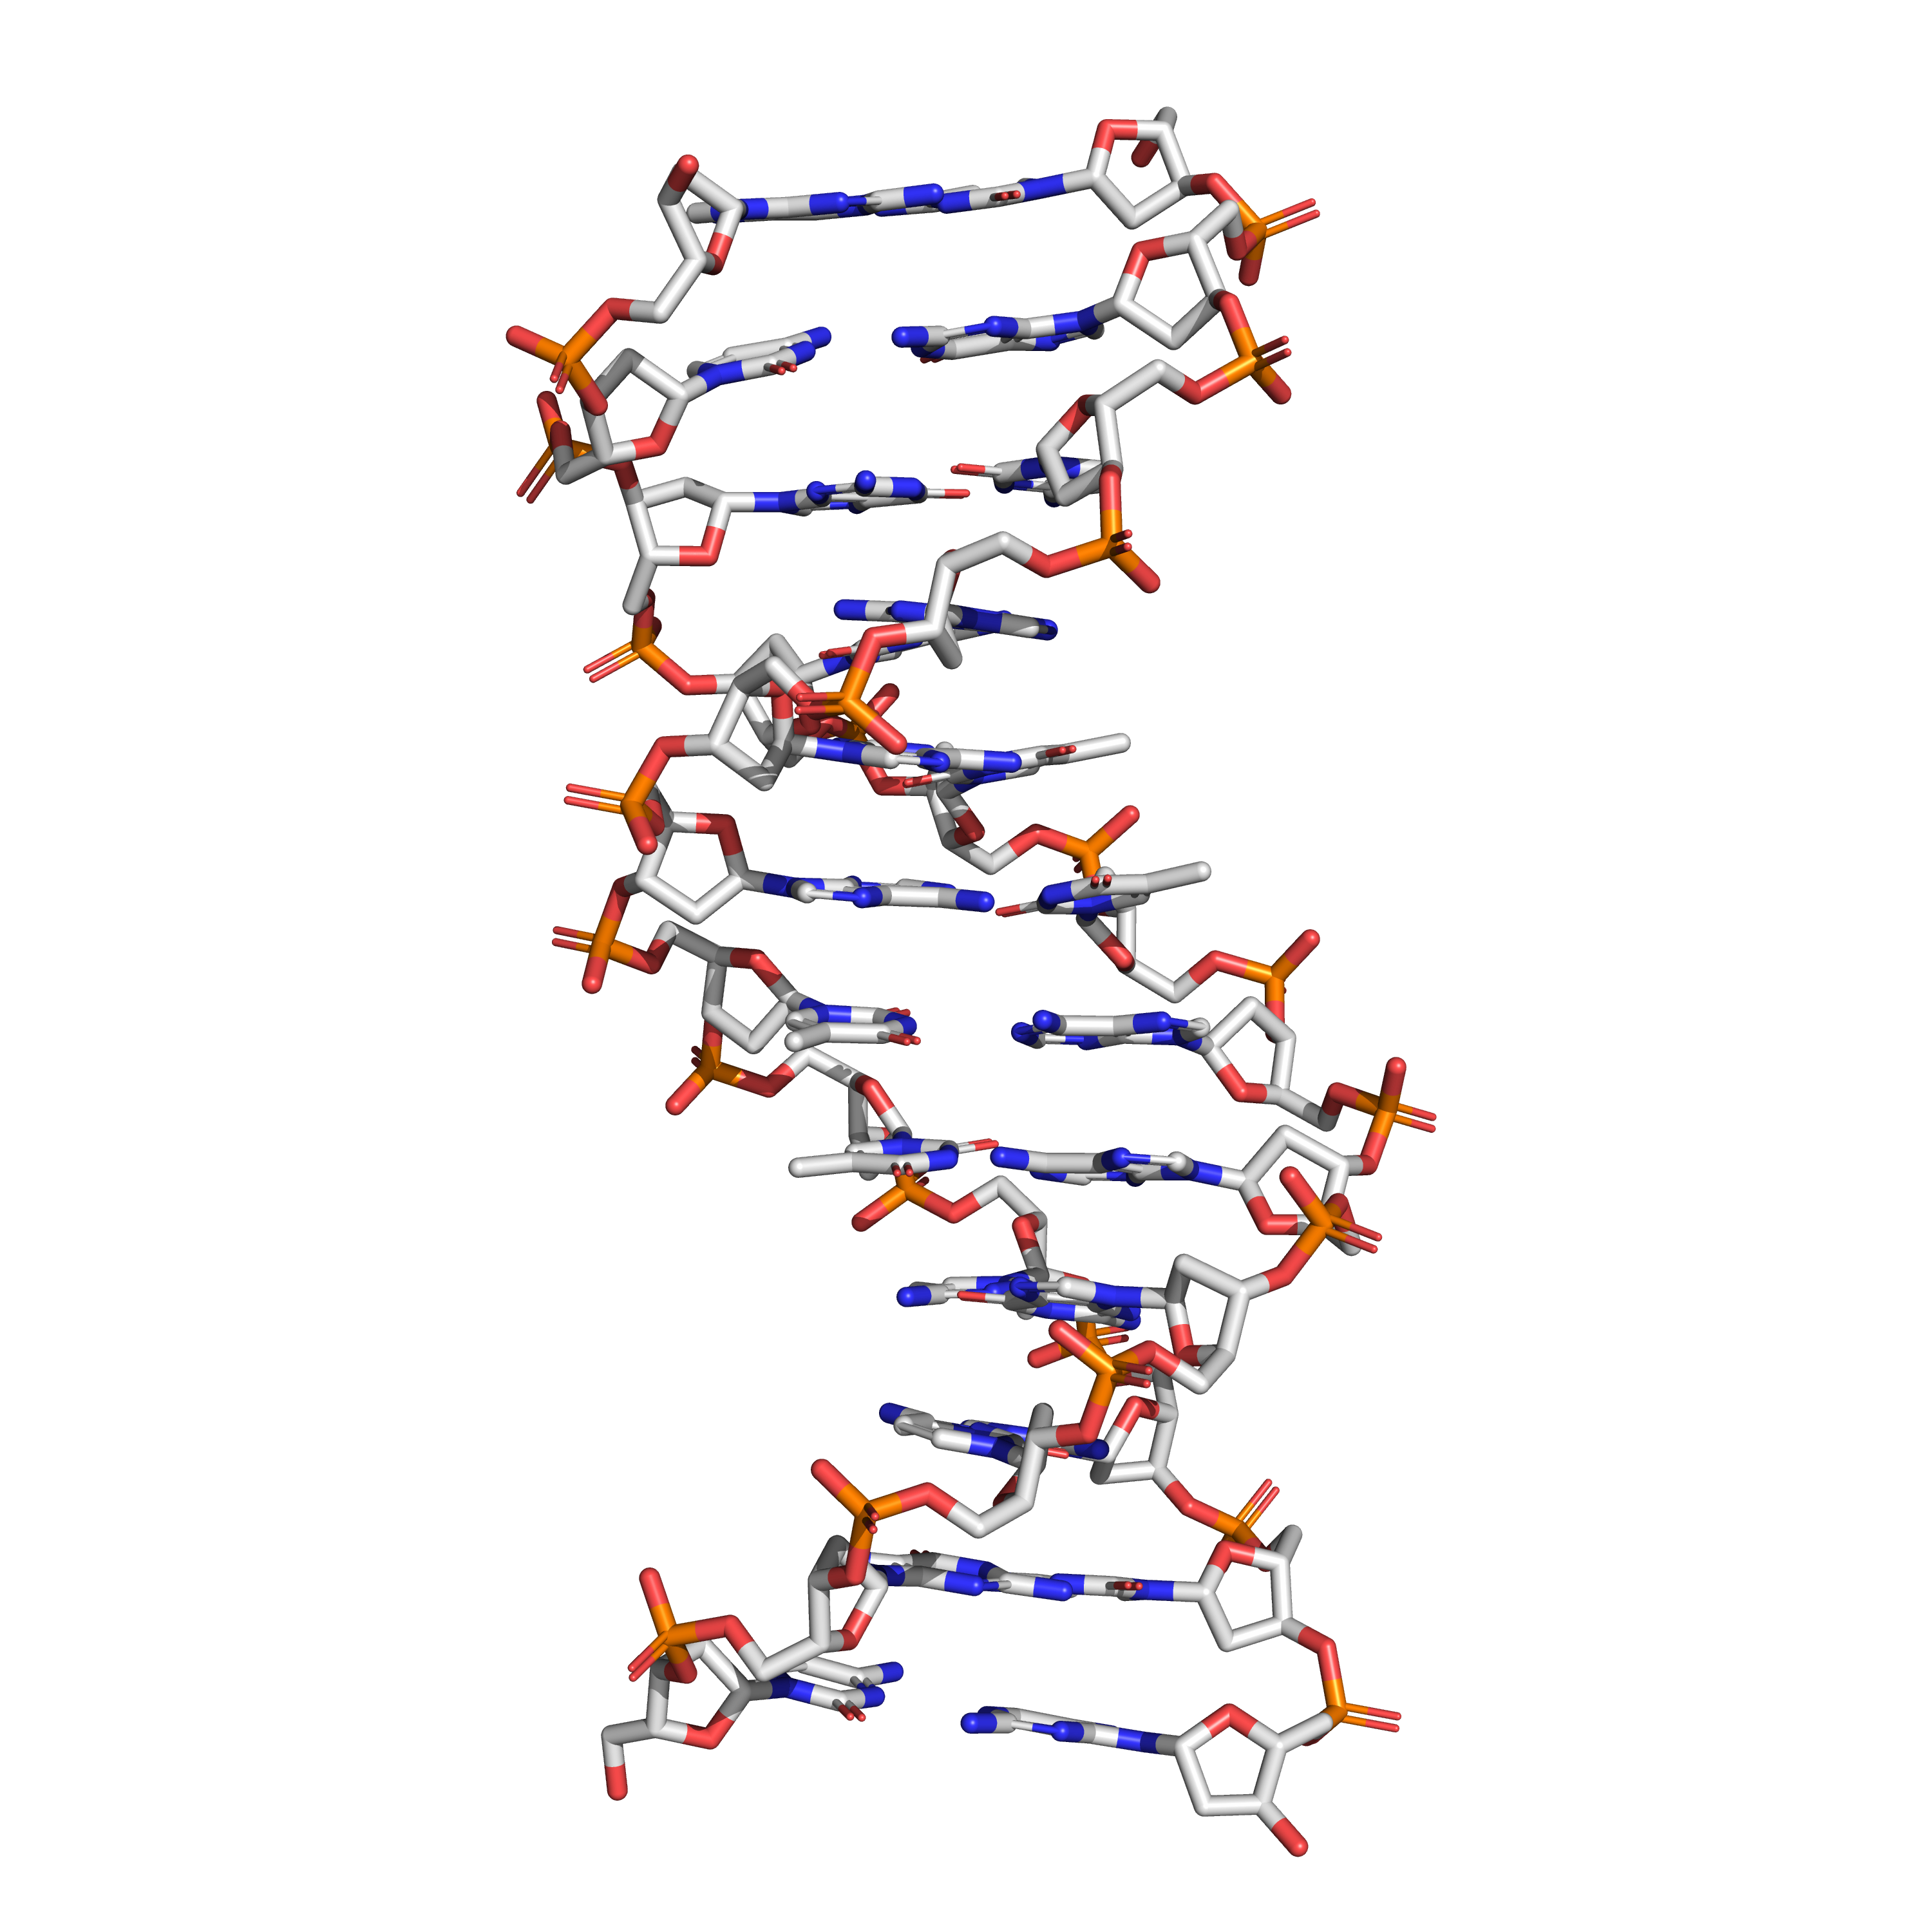
\includegraphics[width=0.7\linewidth]{./figures/dna/dna_licorice} 

}

\caption{The structure of the DNA double helix. A section of DNA. The bases lie horizontally between the two spiraling strands (based on atomic coordinates of \href{https://www.rcsb.org/structure/1bna}{PDB 1bna} rendered with \href{https://www.cgl.ucsf.edu/chimera/}{UCSF Chimera}.)}\label{fig:dnastruc}
\end{figure}

The two DNA strands are also known as polynucleotides as they are composed of simpler monomeric units called nucleotides. Each nucleotide is composed of one of four nitrogen-containing nucleobases (cytosine {[}C{]}, guanine {[}G{]}, adenine {[}A{]} or thymine {[}T{]}), a sugar called deoxyribose, and a phosphate group. The nucleotides are joined to one another in a chain by covalent bonds between the sugar of one nucleotide and the phosphate of the next, resulting in an alternating sugar-phosphate backbone. The nitrogenous bases of the two separate polynucleotide strands are bound together, according to base pairing rules (A with T and C with G), with hydrogen bonds to make double-stranded DNA. The complementary nitrogenous bases are divided into two groups, pyrimidines and purines. In DNA, the pyrimidines are thymine and cytosine; the purines are adenine and guanine.



\begin{figure}

{\centering 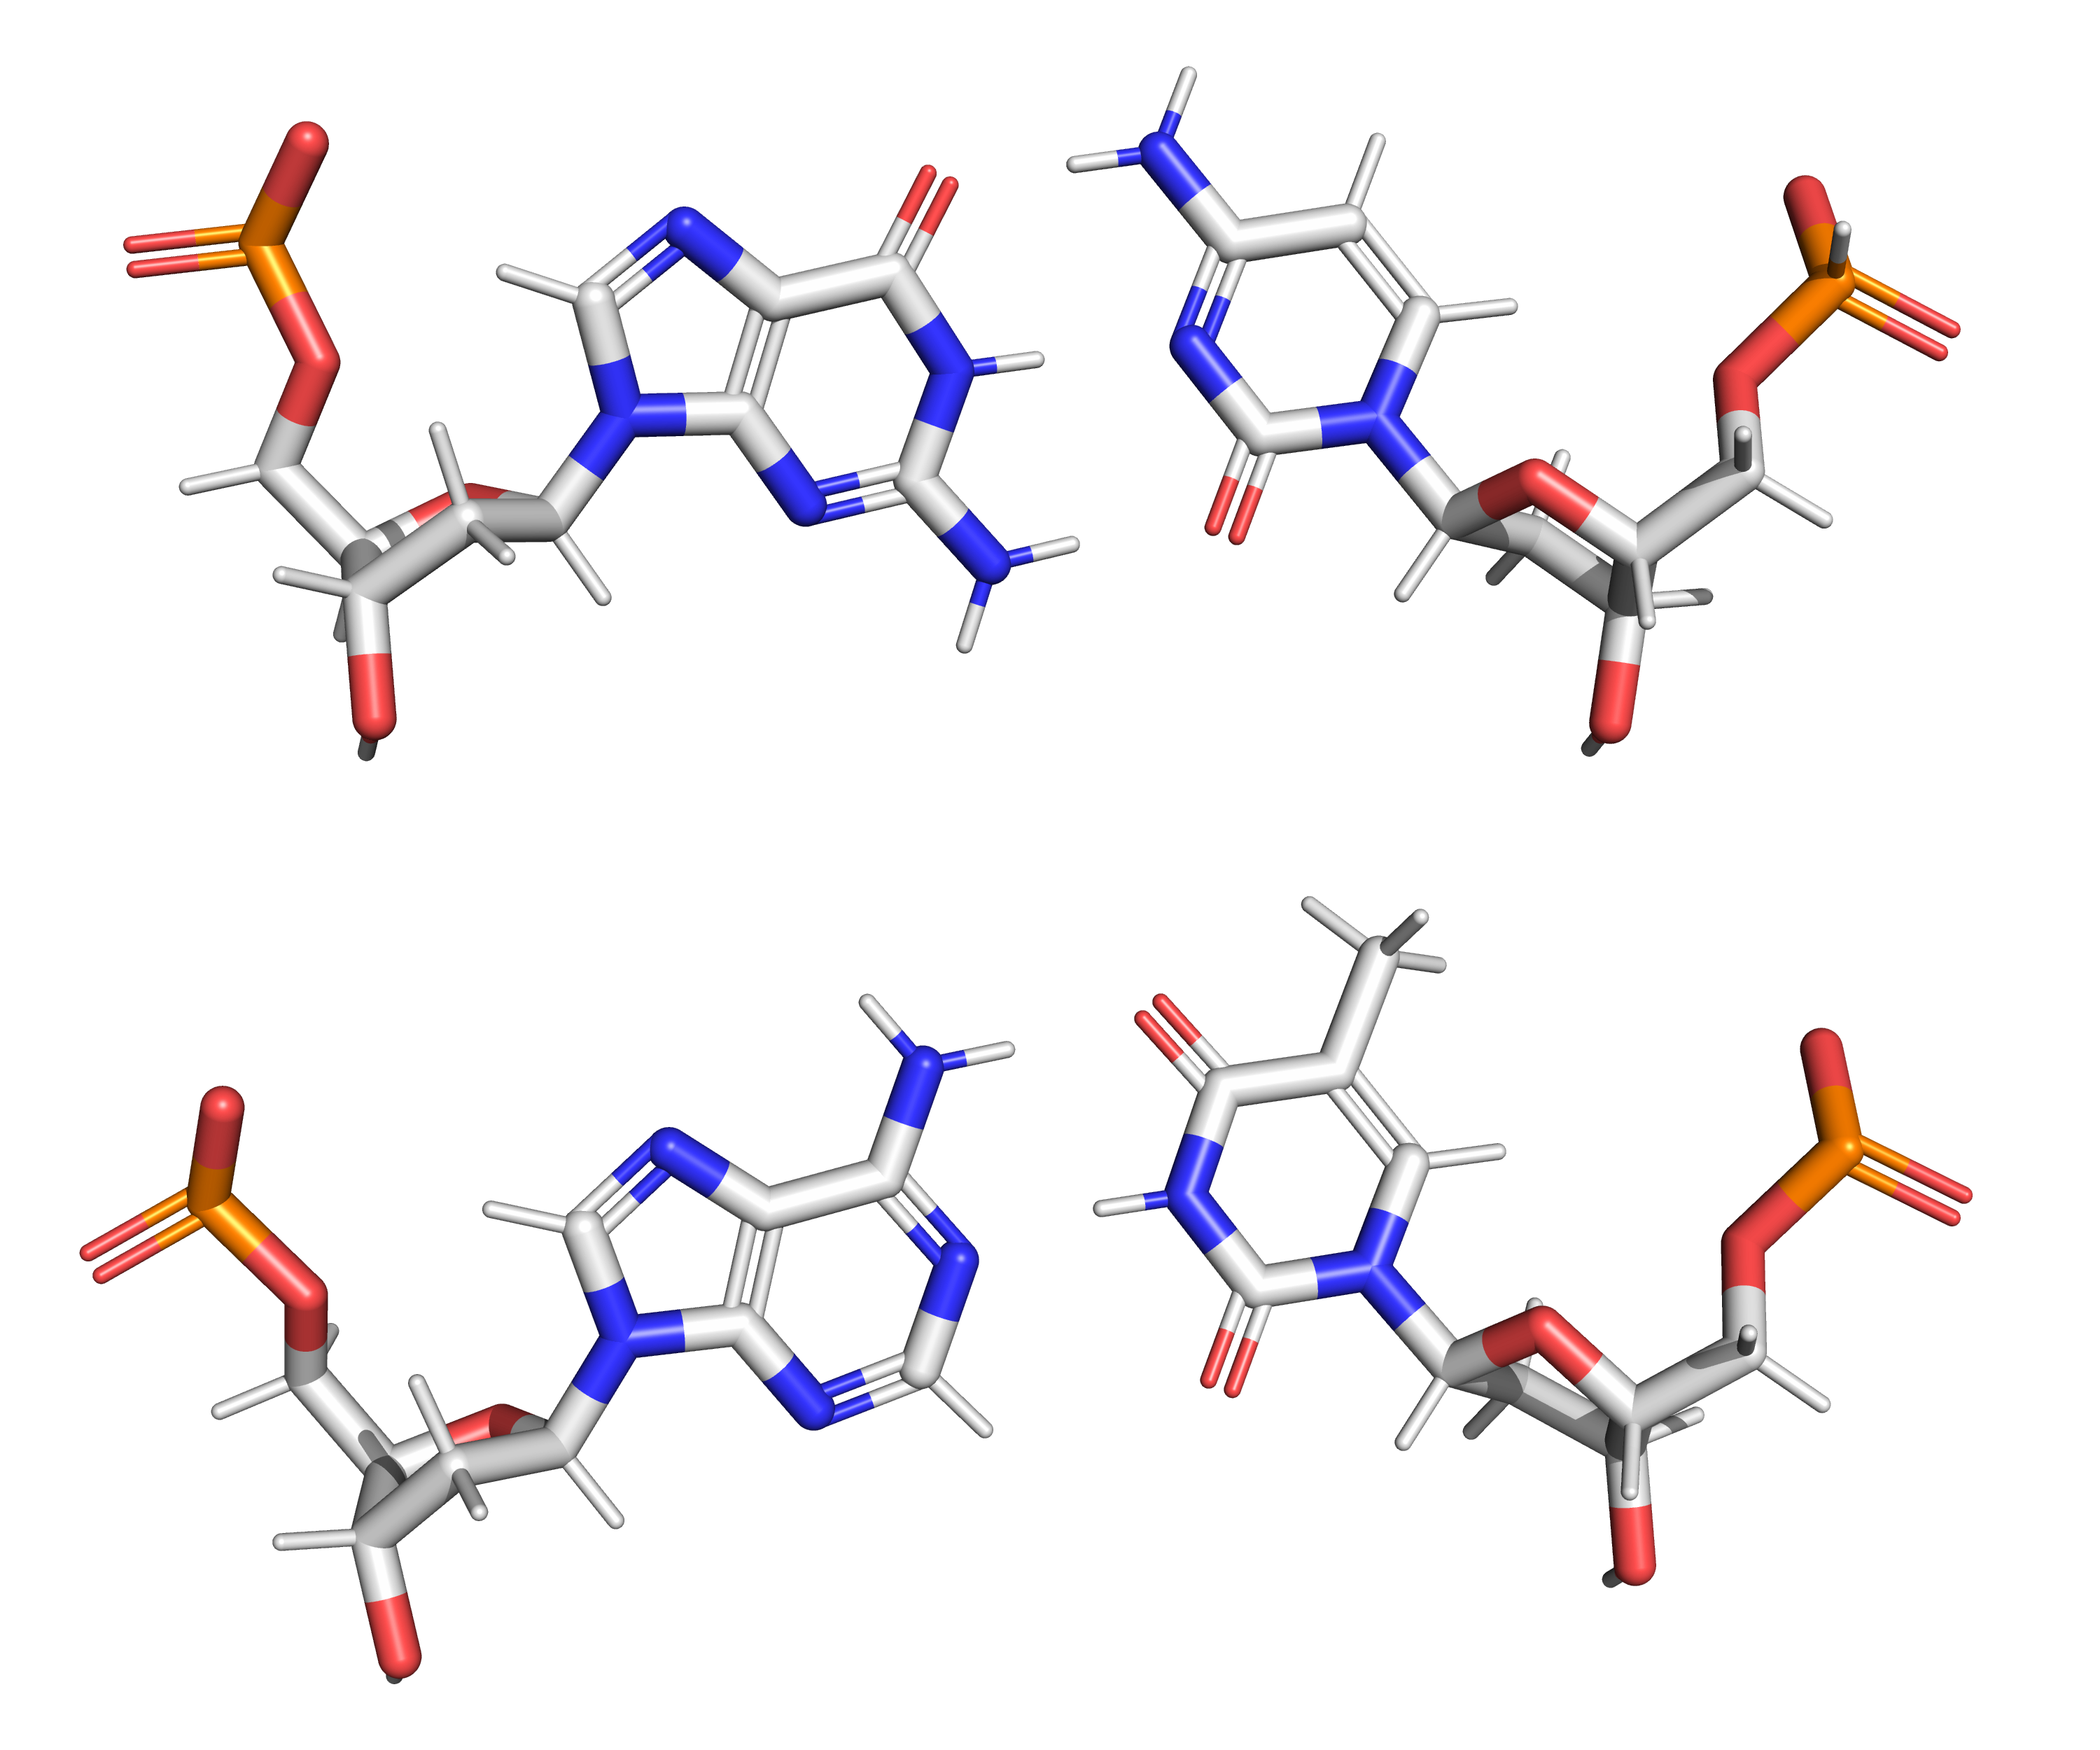
\includegraphics[width=0.7\linewidth]{./figures/dna/bases_hydrogen} 

}

\caption{The structure of the four nucleotides and their base pairing in the DNA double helix. The atoms in the structure are colour-coded by element (based on atomic coordinates of \href{https://www.rcsb.org/structure/1bna}{PDB 1bna} rendered with open source molecular visualization tool PyMol.)}\label{fig:basestruc}
\end{figure}

Both strands of double-stranded DNA store the same biological information. This information is replicated as and when the two strands separate. A large part of DNA (more than 98\% for humans) is non-coding, meaning that these sections do not serve as patterns for protein sequences. The two strands of DNA run in opposite directions to each other and are thus antiparallel. Attached to each sugar is one of four types of nucleobases (informally, bases). It is the sequence of these four nucleobases along the backbone that encodes genetic information. RNA strands are created using DNA strands as a template in a process called transcription, where DNA bases are exchanged for their corresponding bases except in the case of thymine (T), which RNA substitutes for uracil (U). Under the genetic code, these RNA strands specify the sequence of amino acids within proteins in a process called translation.

Within eukaryotic cells, DNA is organized into long structures called chromosomes. Before typical cell division, these chromosomes are duplicated in the process of DNA replication, providing a complete set of chromosomes for each daughter cell. Eukaryotic organisms (animals, plants, fungi and protists) store most of their DNA inside the cell nucleus as nuclear DNA, and some in the mitochondria as mitochondrial DNA or in chloroplasts as chloroplast DNA. In contrast, prokaryotes (bacteria and archaea) store their DNA only in the cytoplasm, in circular chromosomes. Within eukaryotic chromosomes, chromatin proteins, such as histones, compact and organize DNA. These compacting structures guide the interactions between DNA and other proteins, helping control which parts of the DNA are transcribed.

DNA was first isolated by \href{https://en.wikipedia.org/wiki/Friedrich_Miescher}{Friedrich Miescher} in 1869. Its molecular structure was first identified by \href{https://en.wikipedia.org/wiki/Francis_Crick}{Francis Crick} and \href{https://en.wikipedia.org/wiki/James_Watson}{James Watson} at the Cavendish Laboratory within the University of Cambridge in 1953, whose model-building efforts were guided by X-ray diffraction data acquired by \href{https://en.wikipedia.org/wiki/Raymond_Gosling}{Raymond Gosling}, who was a post-graduate student of \href{https://en.wikipedia.org/wiki/Rosalind_Franklin}{Rosalind Franklin}.

\hypertarget{properties}{%
\section{Properties}\label{properties}}

DNA is a long polymer made from repeating units called nucleotides, each of which is usually symbolized by a single letter: either A, T, C, or G. The structure of DNA is dynamic along its length, being capable of coiling into tight loops and other shapes. In all species it is composed of two helical chains, bound to each other by hydrogen bonds. Both chains are coiled around the same axis, and have the same pitch of 34 angstroms (Å) (3.4 nanometres). The pair of chains has a radius of 10 angstroms (1.0 nanometre). According to another study, when measured in a different solution, the DNA chain measured 22 to 26 angstroms wide (2.2 to 2.6 nanometres), and one nucleotide unit measured 3.3 Å (0.33 nm) long. Although each individual nucleotide is very small, a DNA polymer can be very large and contain hundreds of millions, such as in chromosome 1. Chromosome 1 is the largest human chromosome with approximately 220 million base pairs, and would be 85 mm long if straightened.

DNA does not usually exist as a single strand, but instead as a pair of strands that are held tightly together. These two long strands coil around each other, in the shape of a double helix. The nucleotide contains both a segment of the backbone of the molecule (which holds the chain together) and a nucleobase (which interacts with the other DNA strand in the helix). A nucleobase linked to a sugar is called a nucleoside, and a base linked to a sugar and to one or more phosphate groups is called a nucleotide. A biopolymer comprising multiple linked nucleotides (as in DNA) is called a polynucleotide.

The backbone of the DNA strand is made from alternating phosphate and sugar residues. The sugar in DNA is 2-deoxyribose, which is a pentose (five-carbon) sugar. The sugars are joined together by phosphate groups that form phosphodiester bonds between the third and fifth carbon atoms of adjacent sugar rings. These are known as the 3′-end (three prime end), and 5′-end (five prime end) carbons, the prime symbol being used to distinguish these carbon atoms from those of the base to which the deoxyribose forms a glycosidic bond. When imagining DNA, each phosphoryl is normally considered to ``belong'' to the nucleotide whose 5′ carbon forms a bond therewith. Any DNA strand therefore normally has one end at which there is a phosphoryl attached to the 5′ carbon of a ribose (the 5′ phosphoryl) and another end at which there is a free hydroxyl attached to the 3′ carbon of a ribose (the 3′ hydroxyl). The orientation of the 3′ and 5′ carbons along the sugar-phosphate backbone confers directionality (sometimes called polarity) to each DNA strand. In a nucleic acid double helix, the direction of the nucleotides in one strand is opposite to their direction in the other strand: the strands are antiparallel. The asymmetric ends of DNA strands are said to have a directionality of five prime end (5′ ), and three prime end (3′), with the 5′ end having a terminal phosphate group and the 3′ end a terminal hydroxyl group. One major difference between DNA and RNA is the sugar, with the 2-deoxyribose in DNA being replaced by the alternative pentose sugar ribose in RNA.

The DNA double helix is stabilized primarily by two forces: hydrogen bonds between nucleotides and base-stacking interactions among aromatic nucleobases. In the cytosol of the cell, the conjugated pi bonds of nucleotide bases align perpendicular to the axis of the DNA molecule, minimizing their interaction with the solvation shell. The four bases found in DNA are adenine (A), cytosine (C), guanine (G) and thymine (T). These four bases are attached to the sugar-phosphate to form the complete nucleotide, as shown for adenosine monophosphate. Adenine pairs with thymine and guanine pairs with cytosine, forming A-T and G-C base pairs.

\hypertarget{nucleobase-classification}{%
\section{Nucleobase classification}\label{nucleobase-classification}}

The nucleobases are classified into two types: the purines, A and G, which are fused five- and six-membered heterocyclic compounds, and the pyrimidines, the six-membered rings C and T. A fifth pyrimidine nucleobase, uracil (U), usually takes the place of thymine in RNA and differs from thymine by lacking a methyl group on its ring. In addition to RNA and DNA, many artificial nucleic acid analogues have been created to study the properties of nucleic acids, or for use in biotechnology.

\hypertarget{grooves}{%
\section{Grooves}\label{grooves}}

Twin helical strands form the DNA backbone. Another double helix may be found tracing the spaces, or grooves, between the strands (Figure \ref{fig:groove}). These voids are adjacent to the base pairs and may provide a binding site. As the strands are not symmetrically located with respect to each other, the grooves are unequally sized. One groove, the major groove, is 22 angstroms (Å) wide and the other, the minor groove, is 12 Å wide. The width of the major groove means that the edges of the bases are more accessible in the major groove than in the minor groove. As a result, proteins such as transcription factors that can bind to specific sequences in double-stranded DNA usually make contact with the sides of the bases exposed in the major groove. This situation varies in unusual conformations of DNA within the cell (see below), but the major and minor grooves are always named to reflect the differences in size that would be seen if the DNA is twisted back into the ordinary B form.



\begin{figure}

{\centering 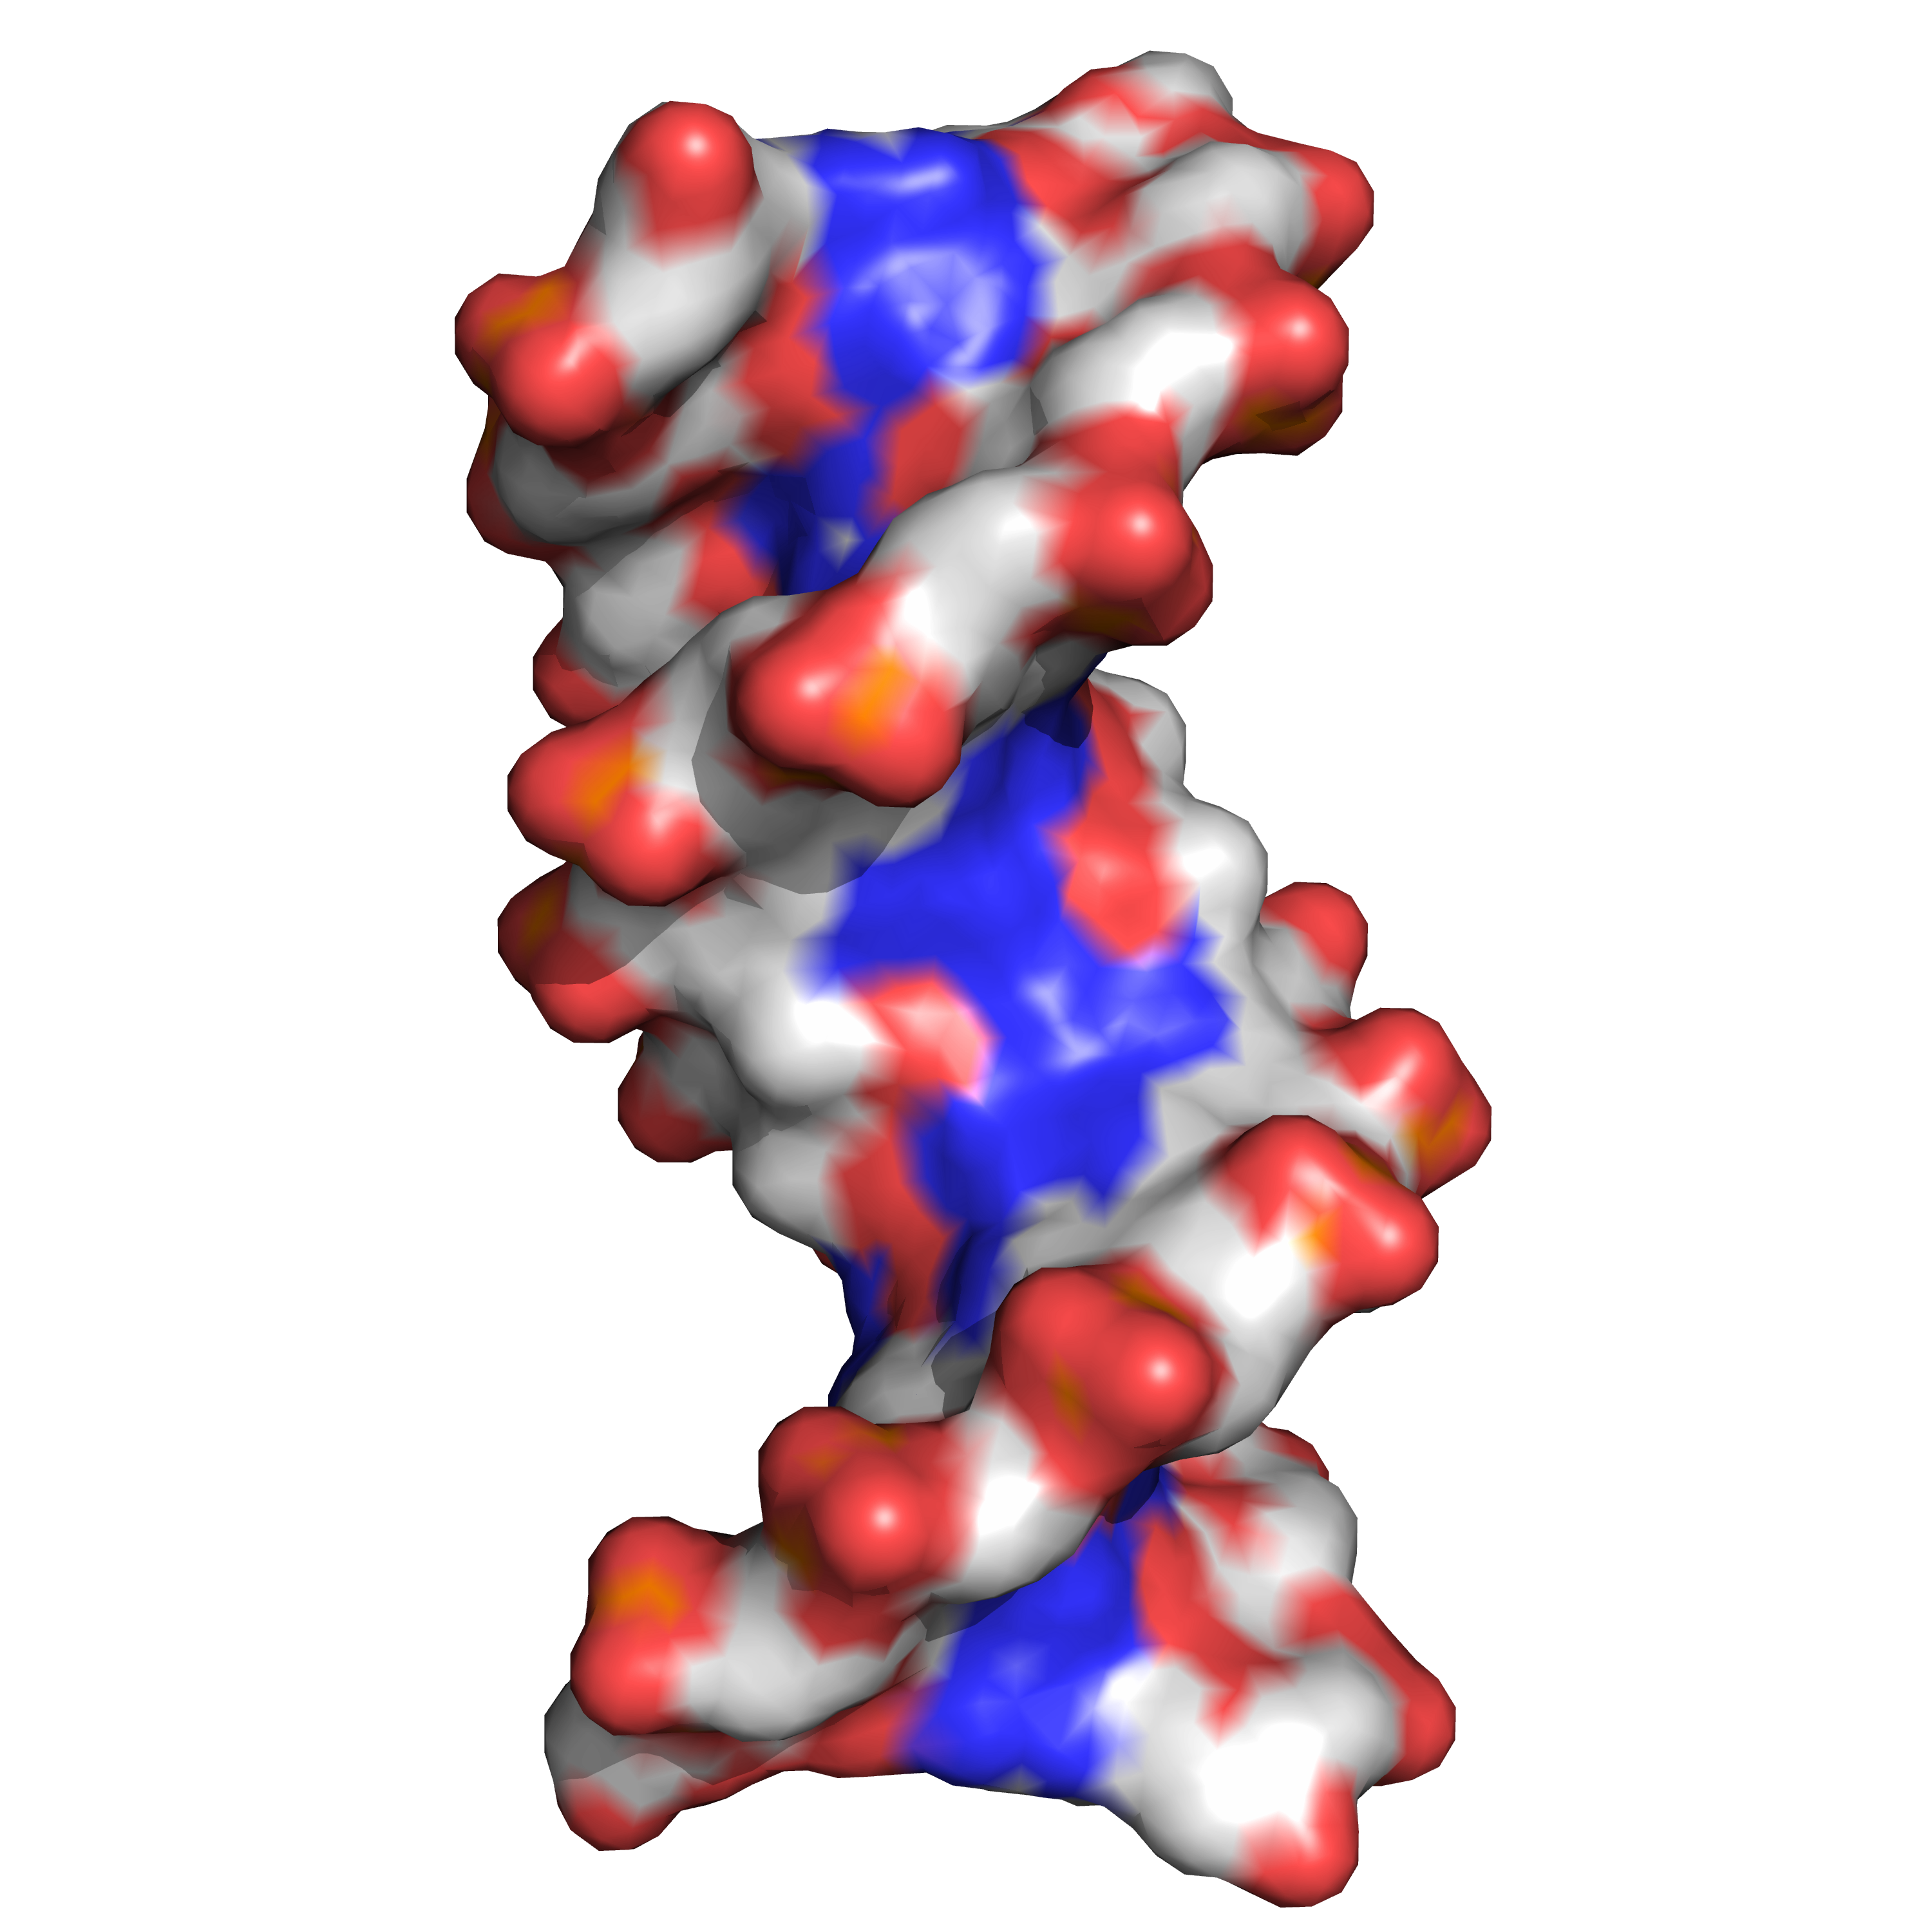
\includegraphics[width=0.7\linewidth]{./figures/dna/dna_solid} 

}

\caption{DNA major and minor grooves. \href{https://www.rcsb.org/structure/1bna}{PDB 1bna} rendered with open source molecular visualization tool PyMol.)}\label{fig:groove}
\end{figure}

\hypertarget{base-pairing}{%
\section{Base pairing}\label{base-pairing}}

In a DNA double helix, each type of nucleobase on one strand bonds with just one type of nucleobase on the other strand. This is called complementary base pairing. Here, purines form hydrogen bonds to pyrimidines, with adenine bonding only to thymine in two hydrogen bonds, and cytosine bonding only to guanine in three hydrogen bonds (Figure \ref{fig:basestruc}). This arrangement of two nucleotides binding together across the double helix is called a Watson-Crick base pair. Another type of base pairing is Hoogsteen base pairing where two hydrogen bonds form between guanine and cytosine. As hydrogen bonds are not covalent, they can be broken and rejoined relatively easily. The two strands of DNA in a double helix can thus be pulled apart like a zipper, either by a mechanical force or high temperature. As a result of this base pair complementarity, all the information in the double-stranded sequence of a DNA helix is duplicated on each strand, which is vital in DNA replication. This reversible and specific interaction between complementary base pairs is critical for all the functions of DNA in organisms.



\begin{figure}

{\centering 
\includegraphics[width=0.7\linewidth]{./figures/dna/Base_pair_GC} 
\includegraphics[width=0.7\linewidth]{./figures/dna/Base_pair_AT} 

}

\caption{Top, a \href{https://commons.wikimedia.org/wiki/File:Base_pair_GC.svg}{GC base pair} with three hydrogen bonds. Bottom, an \href{https://commons.wikimedia.org/wiki/File:Base_pair_AT.svg}{AT base pair} with two hydrogen bonds. Non-covalent hydrogen bonds between the pairs are shown as dashed lines. The two types of base pairs form different numbers of hydrogen bonds, AT forming two hydrogen bonds, and GC forming three hydrogen bonds (see figures, right). DNA with high GC-content is more stable than DNA with low GC-content.}\label{fig:pairing}
\end{figure}

As noted above, most DNA molecules are actually two polymer strands, bound together in a helical fashion by noncovalent bonds; this double-stranded (dsDNA) structure is maintained largely by the intrastrand base stacking interactions, which are strongest for G,C stacks. The two strands can come apart---a process known as melting---to form two single-stranded DNA (ssDNA) molecules. Melting occurs at high temperature, low salt and high pH (ow pH also melts DNA, but since DNA is unstable due to acid depurination, low pH is rarely used).

The stability of the dsDNA form depends not only on the GC-content (\% G,C basepairs) but also on sequence (since stacking is sequence specific) and also length (longer molecules are more stable). The stability can be measured in various ways; a common way is the ``melting temperature'', which is the temperature at which 50\% of the ds molecules are converted to ss molecules; melting temperature is dependent on ionic strength and the concentration of DNA. As a result, it is both the percentage of GC base pairs and the overall length of a DNA double helix that determines the strength of the association between the two strands of DNA. Long DNA helices with a high GC-content have stronger-interacting strands, while short helices with high AT content have weaker-interacting strands. In biology, parts of the DNA double helix that need to separate easily, such as the TATAAT Pribnow box in some promoters, tend to have a high AT content, making the strands easier to pull apart.

In the laboratory, the strength of this interaction can be measured by finding the temperature necessary to break the hydrogen bonds, their melting temperature (also called Tm value). When all the base pairs in a DNA double helix melt, the strands separate and exist in solution as two entirely independent molecules. These single-stranded DNA molecules have no single common shape, but some conformations are more stable than others.

\hypertarget{sense-and-antisense}{%
\section{Sense and antisense}\label{sense-and-antisense}}

A DNA sequence is called a ``sense'' sequence if it is the same as that of a messenger RNA copy that is translated into protein. The sequence on the opposite strand is called the ``antisense'' sequence. Both sense and antisense sequences can exist on different parts of the same strand of DNA (i.e.~both strands can contain both sense and antisense sequences). In both prokaryotes and eukaryotes, antisense RNA sequences are produced, but the functions of these RNAs are not entirely clear. One proposal is that antisense RNAs are involved in regulating gene expression through RNA-RNA base pairing.

A few DNA sequences in prokaryotes and eukaryotes, and more in plasmids and viruses, blur the distinction between sense and antisense strands by having overlapping genes. In these cases, some DNA sequences do double duty, encoding one protein when read along one strand, and a second protein when read in the opposite direction along the other strand. In bacteria, this overlap may be involved in the regulation of gene transcription, while in viruses, overlapping genes increase the amount of information that can be encoded within the small viral genome.

\hypertarget{supercoiling}{%
\section{Supercoiling}\label{supercoiling}}

DNA can be twisted like a rope in a process called DNA supercoiling. With DNA in its ``relaxed'' state, a strand usually circles the axis of the double helix once every 10.4 base pairs, but if the DNA is twisted the strands become more tightly or more loosely wound. If the DNA is twisted in the direction of the helix, this is positive supercoiling, and the bases are held more tightly together. If they are twisted in the opposite direction, this is negative supercoiling, and the bases come apart more easily. In nature, most DNA has slight negative supercoiling that is introduced by enzymes called topoisomerases. These enzymes are also needed to relieve the twisting stresses introduced into DNA strands during processes such as transcription and DNA replication.

\hypertarget{base-modifications-and-dna-packaging}{%
\section{Base modifications and DNA packaging}\label{base-modifications-and-dna-packaging}}

The expression of genes is influenced by how the DNA is packaged in chromosomes, in a structure called chromatin. Base modifications can be involved in packaging, with regions that have low or no gene expression usually containing high levels of methylation of cytosine bases. DNA packaging and its influence on gene expression can also occur by covalent modifications of the histone protein core around which DNA is wrapped in the chromatin structure or else by remodeling carried out by chromatin remodeling complexes (see Chromatin remodeling). There is, further, crosstalk between DNA methylation and histone modification, so they can coordinately affect chromatin and gene expression.

For one example, cytosine methylation produces 5-methylcytosine, which is important for X-inactivation of chromosomes. The average level of methylation varies between organisms---the worm Caenorhabditis elegans lacks cytosine methylation, while vertebrates have higher levels, with up to 1\% of their DNA containing 5-methylcytosine. Despite the importance of 5-methylcytosine, it can deaminate to leave a thymine base, so methylated cytosines are particularly prone to mutations. Other base modifications include adenine methylation in bacteria, the presence of 5-hydroxymethylcytosine in the brain, and the glycosylation of uracil to produce the ``J-base'' in kinetoplastids.

\hypertarget{damage}{%
\section{Damage}\label{damage}}

DNA can be damaged by many sorts of mutagens, which change the DNA sequence. Mutagens include oxidizing agents, alkylating agents and also high-energy electromagnetic radiation such as ultraviolet light and X-rays. The type of DNA damage produced depends on the type of mutagen. For example, UV light can damage DNA by producing thymine dimers, which are cross-links between pyrimidine bases. On the other hand, oxidants such as free radicals or hydrogen peroxide produce multiple forms of damage, including base modifications, particularly of guanosine, and double-strand breaks. A typical human cell contains about 150,000 bases that have suffered oxidative damage. Of these oxidative lesions, the most dangerous are double-strand breaks, as these are difficult to repair and can produce point mutations, insertions, deletions from the DNA sequence, and chromosomal translocations. These mutations can cause cancer. Because of inherent limits in the DNA repair mechanisms, if humans lived long enough, they would all eventually develop cancer. DNA damages that are naturally occurring, due to normal cellular processes that produce reactive oxygen species, the hydrolytic activities of cellular water, etc., also occur frequently. Although most of these damages are repaired, in any cell some DNA damage may remain despite the action of repair processes. These remaining DNA damages accumulate with age in mammalian postmitotic tissues. This accumulation appears to be an important underlying cause of aging.

Many mutagens fit into the space between two adjacent base pairs, this is called intercalation. Most intercalators are aromatic and planar molecules; examples include ethidium bromide, acridines, daunomycin, and doxorubicin. For an intercalator to fit between base pairs, the bases must separate, distorting the DNA strands by unwinding of the double helix. This inhibits both transcription and DNA replication, causing toxicity and mutations. As a result, DNA intercalators may be carcinogens, and in the case of thalidomide, a teratogen. Others such as benzo{[}a{]}pyrene diol epoxide and aflatoxin form DNA adducts that induce errors in replication. Nevertheless, due to their ability to inhibit DNA transcription and replication, other similar toxins are also used in chemotherapy to inhibit rapidly growing cancer cells.

\hypertarget{biological-functions}{%
\section{Biological functions}\label{biological-functions}}

DNA usually occurs as linear chromosomes in eukaryotes, and circular chromosomes in prokaryotes. The set of chromosomes in a cell makes up its genome; the human genome has approximately 3 billion base pairs of DNA arranged into 46 chromosomes. The information carried by DNA is held in the sequence of pieces of DNA called genes. Transmission of genetic information in genes is achieved via complementary base pairing. For example, in transcription, when a cell uses the information in a gene, the DNA sequence is copied into a complementary RNA sequence through the attraction between the DNA and the correct RNA nucleotides. Usually, this RNA copy is then used to make a matching protein sequence in a process called translation, which depends on the same interaction between RNA nucleotides. In alternative fashion, a cell may simply copy its genetic information in a process called DNA replication. The details of these functions are covered in other articles; here the focus is on the interactions between DNA and other molecules that mediate the function of the genome.

\hypertarget{genes-and-genomes}{%
\section{Genes and genomes}\label{genes-and-genomes}}

Genomic DNA is tightly and orderly packed in the process called DNA condensation, to fit the small available volumes of the cell. In eukaryotes, DNA is located in the cell nucleus, with small amounts in mitochondria and chloroplasts. In prokaryotes, the DNA is held within an irregularly shaped body in the cytoplasm called the nucleoid. The genetic information in a genome is held within genes, and the complete set of this information in an organism is called its genotype. A gene is a unit of heredity and is a region of DNA that influences a particular characteristic in an organism. Genes contain an open reading frame that can be transcribed, and regulatorysequences such as promoters and enhancers, which control transcription of the open reading frame.

In many species, only a small fraction of the total sequence of the genome encodes protein. For example, only about 1.5\% of the human genome consists of protein-coding exons, with over 50\% of human DNA consisting of non-coding repetitive sequences. The reasons for the presence of so much noncoding DNA in eukaryotic genomes and the extraordinary differences in genome size, or C-value, among species, represent a long-standing puzzle known as the ``C-value enigma''. However, some DNA sequences that do not code protein may still encode functional non-coding RNA molecules, which are involved in the regulation of gene expression.

Some noncoding DNA sequences play structural roles in chromosomes. Telomeres and centromeres typically contain few genes but are important for the function and stability of chromosomes. An abundant form of noncoding DNA in humans are pseudogenes, which are copies of genes that have been disabled by mutation. These sequences are usually just molecular fossils, although they can occasionally serve as raw genetic material for the creation of new genes through the process of gene duplication and divergence.

\hypertarget{transcription-and-translation}{%
\section{Transcription and translation}\label{transcription-and-translation}}

A gene is a sequence of DNA that contains genetic information and can influence the phenotype of an organism. Within a gene, the sequence of bases along a DNA strand defines a messenger RNA sequence, which then defines one or more protein sequences. The relationship between the nucleotide sequences of genes and the amino-acid sequences of proteins is determined by the rules of translation, known collectively as the genetic code. The genetic code consists of three-letter `words' called codons formed from a sequence of three nucleotides (e.g.~ACT, CAG, TTT).

In transcription, the codons of a gene are copied into messenger RNA by RNA polymerase. This RNA copy is then decoded by a ribosome that reads the RNA sequence by base-pairing the messenger RNA to transfer RNA, which carries amino acids. Since there are 4 bases in 3-letter combinations, there are 64 possible codons (43 combinations). These encode the twenty standard amino acids, giving most amino acids more than one possible codon. There are also three `stop' or `nonsense' codons signifying the end of the coding region; these are the TAA, TGA, and TAG codons.

\hypertarget{replication-1}{%
\section{Replication}\label{replication-1}}

Cell division is essential for an organism to grow, but, when a cell divides, it must replicate the DNA in its genome so that the two daughter cells have the same genetic information as their parent. The double-stranded structure of DNA provides a simple mechanism for DNA replication. Here, the two strands are separated and then each strand's complementary DNA sequence is recreated by an enzyme called DNA polymerase. This enzyme makes the complementary strand by finding the correct base through complementary base pairing and bonding it onto the original strand. As DNA polymerases can only extend a DNA strand in a 5′ to 3′ direction, different mechanisms are used to copy the antiparallel strands of the double helix. In this way, the base on the old strand dictates which base appears on the new strand, and the cell ends up with a perfect copy of its DNA.

\hypertarget{interactions-with-proteins}{%
\section{Interactions with proteins}\label{interactions-with-proteins}}

All the functions of DNA depend on interactions with proteins. These protein interactions can be non-specific, or the protein can bind specifically to a single DNA sequence. Enzymes can also bind to DNA and of these, the polymerases that copy the DNA base sequence in transcription and DNA replication are particularly important.

\hypertarget{dna-binding-proteins}{%
\section{DNA-binding proteins}\label{dna-binding-proteins}}

Structural proteins that bind DNA are well-understood examples of non-specific DNA-protein interactions. Within chromosomes, DNA is held in complexes with structural proteins. These proteins organize the DNA into a compact structure called chromatin. In eukaryotes, this structure involves DNA binding to a complex of small basic proteins called histones, while in prokaryotes multiple types of proteins are involved. The histones form a disk-shaped complex called a nucleosome, which contains two complete turns of double-stranded DNA wrapped around its surface. These non-specific interactions are formed through basic residues in the histones, making ionic bonds to the acidic sugar-phosphate backbone of the DNA, and are thus largely independent of the base sequence. Chemical modifications of these basic amino acid residues include methylation, phosphorylation, and acetylation. These chemical changes alter the strength of the interaction between the DNA and the histones, making the DNA more or less accessible to transcription factors and changing the rate of transcription. Other non-specific DNA-binding proteins in chromatin include the high-mobility group proteins, which bind to bent or distorted DNA. These proteins are important in bending arrays of nucleosomes and arranging them into the larger structures that make up chromosomes.

A distinct group of DNA-binding proteins is the DNA-binding proteins that specifically bind single-stranded DNA. In humans, replication protein A is the best-understood member of this family and is used in processes where the double helix is separated, including DNA replication, recombination, and DNA repair. These binding proteins seem to stabilize single-stranded DNA and protect it from forming stem-loops or being degraded by nucleases.

In contrast, other proteins have evolved to bind to particular DNA sequences. The most intensively studied of these are the various transcription factors, which are proteins that regulate transcription. Each transcription factor binds to one particular set of DNA sequences and activates or inhibits the transcription of genes that have these sequences close to their promoters. The transcription factors do this in two ways. Firstly, they can bind the RNA polymerase responsible for transcription, either directly or through other mediator proteins; this locates the polymerase at the promoter and allows it to begin transcription. Alternatively, transcription fctors can bind enzymes that modify the histones at the promoter. This changes the accessibility of the DNA template to the polymerase.

As these DNA targets can occur throughout an organism's genome, changes in the activity of one type of transcription factor can affect thousands of genes. Consequently, these proteins are often the targets of the signal transduction processes that control responses to environmental changes or cellular differentiation and development. The specificity of these transcription factors' interactions with DNA come from the proteins making multiple contacts to the edges of the DNA bases, allowing them to ``read'' the DNA sequence. Most of these base-interactions are made in the major groove, where the bases are most accessible.

\hypertarget{dna-modifying-enzymes}{%
\section{DNA-modifying enzymes}\label{dna-modifying-enzymes}}

\hypertarget{nucleases-and-ligases}{%
\subsection{Nucleases and ligases}\label{nucleases-and-ligases}}

Nucleases are enzymes that cut DNA strands by catalyzing the hydrolysis of the phosphodiester bonds. Nucleases that hydrolyse nucleotides from the ends of DNA strands are called exonucleases, while endonucleases cut within strands. The most frequently used nucleases in molecular biology are the restriction endonucleases, which cut DNA at specific sequences. For instance, the EcoRV enzyme shown to the left recognizes the 6-base sequence 5′-GATATC-3′ and makes a cut at the horizontal line. In nature, these enzymes protect bacteria against phage infection by digesting the phage DNA when it enters the bacterial cell, actng as part of the restriction modification system. In technology, these sequence-specific nucleases are used in molecular cloning and DNA fingerprinting.

Enzymes called DNA ligases can rejoin cut or broken DNA strands. Ligases are particularly important in lagging strand DNA replication, as they join together the short segments of DNA produced at the replication fork into a complete copy of the DNA template. They are also used in DNA repair and genetic recombination.

\hypertarget{topoisomerases-and-helicases}{%
\section{Topoisomerases and helicases}\label{topoisomerases-and-helicases}}

Topoisomerases are enzymes with both nuclease and ligase activity. These proteins change the amount of supercoiling in DNA. Some of these enzymes work by cutting the DNA helix and allowing one section to rotate, thereby reducing its level of supercoiling; the enzyme then seals the DNA break. Other types of these enzymes are capable of cutting one DNA helix and then passing a second strand of DNA through this break, before rejoining the helix. Topoisomerases are required for many processes involving DNA, such as DNA replication and transcription.

Helicases are proteins that are a type of molecular motor. They use the chemical energy in nucleoside triphosphates, predominantly adenosine triphosphate (ATP), to break hydrogen bonds between bases and unwind the DNA double helix into single strands. These enzymes are essential for most processes where enzymes need to access the DNA bases.

\hypertarget{polymerases}{%
\section{Polymerases}\label{polymerases}}

Polymerases are enzymes that synthesize polynucleotide chains from nucleoside triphosphates. The sequence of their products is created based on existing polynucleotide chains---which are called templates. These enzymes function by repeatedly adding a nucleotide to the 3′ hydroxyl group at the end of the growing polynucleotide chain. As a consequence, all polymerases work in a 5′ to 3′ direction. In the active site of these enzymes, the incoming nucleoside triphosphate base-pairs to the template: this allows polymerases to accurately synthesize the complementary strand of their template. Polymerases are classified according to the type of template that they use.

In DNA replication, DNA-dependent DNA polymerases make copies of DNA polynucleotide chains. To preserve biological information, it is essential that the sequence of bases in each copy are precisely complementary to the sequence of bases in the template strand. Many DNA polymerases have a proofreading activity. Here, the polymerase recognizes the occasional mistakes in the synthesis reaction by the lack of base pairing between the mismatched nucleotides. If a mismatch is detected, a 3′ to 5′ exonuclease activity is activated and the incorrect base removed. In most organisms, DNA polymerases function in a large complex called the replisome that contains multiple accessory subunits, such as the DNA clamp or helicases.

RNA-dependent DNA polymerases are a specialized class of polymerases that copy the sequence of an RNA strand into DNA. They include reverse transcriptase, which is a viral enzyme involved in the infection of cells by retroviruses, and telomerase, which is required for the replication of telomeres. For example, HIV reverse transcriptase is an enzyme for AIDS virus replication. Telomerase is an unusual polymerase because it contains its own RNA template as part of its structure. It synthesizes telomeres at the ends of chromosomes. Telomeres prevent fusion of the ends of neighboring chromosomes and protect chromosome ends from damage.

Transcription is carried out by a DNA-dependent RNA polymerase that copies the sequence of a DNA strand into RNA. To begin transcribing a gene, the RNA polymerase binds to a sequence of DNA called a promoter and separates the DNA strands. It then copies the gene sequence into a messenger RNA transcript until it reaches a region of DNA called the terminator, where it halts and detaches from the DNA. As with human DNA-dependent DNA polymerases, RNA polymerase II, the enzyme that transcribes most of the genes in the human genome, operates as part of a large protein complex with multiple regulatory and accessory subunits.

\hypertarget{genetic-recombination}{%
\section{Genetic recombination}\label{genetic-recombination}}

A DNA helix usually does not interact with other segments of DNA, and in human cells, the different chromosomes even occupy separate areas in the nucleus called ``chromosome territories''. This physical separation of different chromosomes is important for the ability of DNA to function as a stable repository for information, as one of the few times chromosomes interact is in chromosomal crossover which occurs during sexual reproduction, when genetic recombination occurs. Chromosomal crossover is when two DNA helices break, swap a section and then rejoin.

Recombination allows chromosomes to exchange genetic information and produces new combinations of genes, which increases the efficiency of natural selection and can be important in the rapid evolution of new proteins. Genetic recombination can also be involved in DNA repair, particularly in the cell's response to double-strand breaks.

The most common form of chromosomal crossover is homologous recombination, where the two chromosomes involved share very similar sequences. Non-homologous recombination can be damaging to cells, as it can produce chromosomal translocations and genetic abnormalities. The recombination reaction is catalyzed by enzymes known as recombinases, such as RAD51. The first step in recombination is a double-stranded break caused by either an endonuclease or damage to the DNA. A series of steps catalyzed in part by the recombinase then leads to joining of the two helices by at least one Holliday junction, in which a segment of a single strand in each helix is annealed to the complementary strand in the other helix. The Holliday junction is a tetrahedral junction structure that can be moved along the pair of chromosomes, swapping one strand for another. The recombination reaction is then halted by cleavage of the junction and re-ligation of the released DNA. Only strands of like polarity exchange DNA during recombination. There are two types of cleavage: east-west cleavage and north-south cleavage. The north-south cleavage nicks both strands of DNA, while the east-west cleavage has one strand of DNA intact. The formation of a Holliday junction during recombination makes it possible for genetic diversity, genes to exchange on chromosomes, and expression of wild-type viral genomes.

\hypertarget{evolution}{%
\section{Evolution}\label{evolution}}

Further information: RNA world hypothesis
DNA contains the genetic information that allows all forms of life to function, grow and reproduce. However, it is unclear how long in the 4-billion-year history of life DNA has performed this function, as it has been proposed that the earliest forms of life may have used RNA as their genetic material. RNA may have acted as the central part of early cell metabolism as it can both transmit genetic information and carry out catalysis as part of ribozymes. This ancient RNA world where nucleic acid would have been used for both catalysis and genetics may have influenced the evolution of the current genetic code based on four nucleotide bases. This would occur, since the number of different bases in such an organism is a trade-off between a small number of bases increasing replication accuracy and a large number of bases increasing the catalytic efficiency of ribozymes. However, there is no direct evidence of ancient genetic systems, as recovery of DNA from most fossils is impossible because DNA survives in the environment for less than one million years, and slowly degrades into short fragments in solution. Claims for older DNA have been made, most notably a report of the isolation of a viable bacterium from a salt crystal 250 million years old, but these claims are controversial.

Building blocks of DNA (adenine, guanine, and related organic molecules) may have been formed extraterrestrially in outer space. Complex DNA and RNA organic compounds of life, including uracil, cytosine, and thymine, have also been formed in the laboratory under conditions mimicking those found in outer space, using starting chemicals, such as pyrimidine, found in meteorites. Pyrimidine, like polycyclic aromatic hydrocarbons (PAHs), the most carbon-rich chemical found in the universe, may have been formed in red giants or in interstellar cosmic dust and gas clouds.

\hypertarget{genetic-engineering}{%
\section{Genetic engineering}\label{genetic-engineering}}

Further information: Molecular biology, Nucleic acid methods, and Genetic engineering
Methods have been developed to purify DNA from organisms, such as phenol-chloroform extraction, and to manipulate it in the laboratory, such as restriction digests and the polymerase chain reaction. Modern biology and biochemistry make intensive use of these techniques in recombinant DNA technology. Recombinant DNA is a man-made DNA sequence that has been assembled from other DNA sequences. They can be transformed into organisms in the form of plasmids or in the appropriate format, by using a viral vector. The genetically modified organisms produced can be used to produce products such as recombinant proteins, used in medical research, or be grown in agriculture.

\hypertarget{dna-profiling}{%
\section{DNA profiling}\label{dna-profiling}}

Further information: DNA profiling
Forensic scientists can use DNA in blood, semen, skin, saliva or hair found at a crime scene to identify a matching DNA of an individual, such as a perpetrator. This process is formally termed DNA profiling, also called DNA fingerprinting. In DNA profiling, the lengths of variable sections of repetitive DNA, such as short tandem repeats and minisatellites, are compared between people. This method is usually an extremely reliable technique for identifying a matching DNA. However, identification can be complicated if the scene is contaminated with DNA from several people. DNA profiling was developed in 1984 by British geneticist Sir Alec Jeffreys, and first used in forensic science to convict Colin Pitchfork in the 1988 Enderby murders case.

The development of forensic science and the ability to now obtain genetic matching on minute samples of blood, skin, saliva, or hair has led to re-examining many cases. Evidence can now be uncovered that was scientifically impossible at the time of the original examination. Combined with the removal of the double jeopardy law in some places, this can allow cases to be reopened where prior trials have failed to produce sufficient evidence to convince a jury. People charged with serious crimes may be required to provide a sample of DNA for matching purposes. The most obvious defense to DNA matches obtained forensically is to claim that cross-contamination of evidence has occurred. This has resulted in meticulous strict handling procedures with new cases of serious crime.

DNA profiling is also used successfully to positively identify victims of mass casualty incidents, bodies or body parts in serious accidents, and individual victims in mass war graves, via matching to family members.

DNA profiling is also used in DNA paternity testing to determine if someone is the biological parent or grandparent of a child with the probability of parentage is typically 99.99\% when the alleged parent is biologically related to the child. Normal DNA sequencing methods happen after birth, but there are new methods to test paternity while a mother is still pregnant.

\hypertarget{rna}{%
\section{RNA}\label{rna}}

\href{https://en.wikipedia.org/wiki/RNA}{Ribonucleic acid (RNA)} is a polymeric molecule essential in various biological roles in coding, decoding, regulation and expression of genes. RNA and DNA are nucleic acids, and, along with lipids, proteins and carbohydrates, constitute the four major macromolecules essential for all known forms of life. Like DNA, RNA is assembled as a chain of nucleotides, but unlike DNA it is more often found in nature as a single-strand folded onto itself, rather than a paired double-strand. Cellular organisms use messenger RNA (mRNA) to convey genetic information (using the nitrogenous bases of guanine, uracil, adenine, and cytosine, denoted by the letters G, U, A, and C) tat directs synthesis of specific proteins. Many viruses encode their genetic information using an RNA genome.

Some RNA molecules play an active role within cells by catalyzing biological reactions, controlling gene expression, or sensing and communicating responses to cellular signals. One of these active processes is protein synthesis, a universal function in which RNA molecules direct the synthesis of proteins on ribosomes. This process uses transfer RNA (tRNA) molecules to deliver amino acids to the ribosome, where ribosomal RNA (rRNA) then links amino acids together to form coded proteins.

\hypertarget{comparison-with-dna}{%
\section{Comparison with DNA}\label{comparison-with-dna}}

The chemical structure of RNA is very similar to that of DNA, but differs in three primary ways:

\begin{itemize}
\tightlist
\item
  Unlike double-stranded DNA, RNA is a single-stranded molecule in many of its biological roles and consists of much shorter chains of nucleotides. However, a single RNA molecule can, by complementary base pairing, form intrastrand double helixes, as in tRNA.
\item
  While the sugar-phosphate ``backbone'' of DNA contains deoxyribose, RNA contains ribose instead. Ribose has a hydroxyl group attached to the pentose ring in the 2' position, whereas deoxyribose does not. The hydroxyl groups in the ribose backbone make RNA more chemically labile than DNA by lowering the activation energy of hydrolysis.
\item
  The complementary base to adenine in DNA is thymine, whereas in RNA, it is uracil, which is an unmethylated form of thymine.
\end{itemize}

Like DNA, most biologically active RNAs, including mRNA, tRNA, rRNA, snRNAs, and other non-coding RNAs, contain self-complementary sequences that allow parts of the RNA to fold and pair with itself to form double helices. Analysis of these RNAs has revealed that they are highly structured. Unlike DNA, their structures do not consist of long double helices, but rather collections of short helices packed together into structures akin to proteins. In this fashion, RNAs can achieve chemical catalysis (like enzymes). For instance, determination of the structure of the ribosome---an RNA-protein complex that catalyzes peptide bond formation---revealed that its active site is composed entirely of RNA.

\hypertarget{structure}{%
\section{Structure}\label{structure}}

Each nucleotide in RNA contains a ribose sugar, with carbons numbered 1' through 5'. A base is attached to the 1' position, in general, adenine (A), cytosine (C), guanine (G), or uracil (U). Adenine and guanine are purines, cytosine and uracil are pyrimidines. A phosphate group is attached to the 3' position of one ribose and the 5' position of the next. The phosphate groups have a negative charge each, making RNA a charged molecule (polyanion). The bases form hydrogen bonds between cytosine and guanine, between adenine and uracil and between guanine and uracil. However, other interactions are possible, such as a group of adenine bases binding to each other in a bulge, or the GNRA tetraloop that has a guanine--adenine base-pair.

An important structural component of RNA that distinguishes it from DNA is the presence of a hydroxyl group at the 2' position of the ribose sugar. The presence of this functional group causes the helix to mostly take the A-form geometry, although in single strand dinucleotide contexts, RNA can rarely also adopt the B-form most commonly observed in DNA. The A-form geometry results in a very deep and narrow major groove and a shallow and wide minor groove. A second consequence of the presence of the 2'-hydroxyl group is that in conformationally flexible regions of an RNA molecule (that is, not involved in formation of a double helix), it can chemically attack the adjacent phosphodiester bond to cleave the backbone.

RNA is transcribed with only four bases (adenine, cytosine, guanine and uracil), but these bases and attached sugars can be modified in numerous ways as the RNAs mature. Pseudouridine (Ψ), in which the linkage between uracil and ribose is changed from a C--N bond to a C--C bond, and ribothymidine (T) are found in various places (the most notable ones being in the TΨC loop of tRNA). Another notable modified base is hypoxanthine, a deaminated adenine base whose nucleoside is called inosine (I). Inosine plays a key role in the wobble hypothesis of the genetic code.

There are more than 100 other naturally occurring modified nucleosides. The greatest structural diversity of modifications can be found in tRNA, while pseudouridine and nucleosides with 2'-O-methylribose often present in rRNA are the most common. The specific roles of many of these modifications in RNA are not fully understood. However, it is notable that, in ribosomal RNA, many of the post-transcriptional modifications occur in highly functional regions, such as the peptidyl transferase center and the subunit interface, implying that they are important for normal function.

The functional form of single-stranded RNA molecules, just like proteins, frequently requires a specific tertiary structure. The scaffold for this structure is provided by secondary structural elements that are hydrogen bonds within the molecule. This leads to several recognizable ``domains'' of secondary structure like hairpin loops, bulges, and internal loops. Since RNA is charged, metal ions such as Mg2+ are needed to stabilise many secondary and tertiary structures.

The naturally occurring enantiomer of RNA is D-RNA composed of D-ribonucleotides. All chirality centers are located in the D-ribose. By the use of L-ribose or rather L-ribonucleotides, L-RNA can be synthesized. L-RNA is much more stable against degradation by RNase.

Like other structured biopolymers such as proteins, one can define topology of a folded RNA molecule. This is often done based on arrangement of intra-chain contacts within a folded RNA, termed as circuit topology.

\hypertarget{synthesis}{%
\section{Synthesis}\label{synthesis}}

Synthesis of RNA is usually catalyzed by an enzyme---RNA polymerase---using DNA as a template, a process known as transcription. Initiation of transcription begins with the binding of the enzyme to a promoter sequence in the DNA (usually found ``upstream'' of a gene). The DNA double helix is unwound by the helicase activity of the enzyme. The enzyme then progresses along the template strand in the 3' to 5' direction, synthesizing a complementary RNA molecule with elongation occurring in the 5' to 3' direction. The DNA sequence also dictates where termination of RNA synthesis will occur.

Primary transcript RNAs are often modified by enzymes after transcription. For example, a poly(A) tail and a 5' cap are added to eukaryotic pre-mRNA and introns are removed by the spliceosome.

There are also a number of RNA-dependent RNA polymerases that use RNA as their template for synthesis of a new strand of RNA. For instance, a number of RNA viruses (such as poliovirus) use this type of enzyme to replicate their genetic material. Also, RNA-dependent RNA polymerase is part of the RNA interference pathway in many organisms.

\hypertarget{types-of-rna}{%
\section{Types of RNA}\label{types-of-rna}}

Messenger RNA (mRNA) is the RNA that carries information from DNA to the ribosome, the sites of protein synthesis (translation) in the cell. The coding sequence of the mRNA determines the amino acid sequence in the protein that is produced. However, many RNAs do not code for protein (about 97\% of the transcriptional output is non-protein-coding in eukaryotes).

These so-called non-coding RNAs (``ncRNA'') can be encoded by their own genes (RNA genes), but can also derive from mRNA introns. The most prominent examples of non-coding RNAs are transfer RNA (tRNA) and ribosomal RNA (rRNA), both of which are involved in the process of translation. There are also non-coding RNAs involved in gene regulation, RNA processing and other roles. Certain RNAs are able to catalyse chemical reactions such as cutting and ligating other RNA molecules, and the catalysis of peptide bond formation in the ribosome; these are known as ribozymes.

\hypertarget{in-length}{%
\section{In length}\label{in-length}}

According to the length of RNA chain, RNA includes small RNA and long RNA. Usually, small RNAs are shorter than 200 nt in length, and long RNAs are greater than 200 nt long. Long RNAs, also called large RNAs, mainly include long non-coding RNA (lncRNA) and mRNA. Small RNAs mainly include 5.8S ribosomal RNA (rRNA), 5S rRNA, transfer RNA (tRNA), microRNA (miRNA), small interfering RNA (siRNA), small nucleolar RNA (snoRNAs), Piwi-interacting RNA (piRNA), tRNA-derived small RNA (tsRNA) and small rDNA-derived RNA (srRNA).

\hypertarget{in-translation}{%
\section{In translation}\label{in-translation}}

Messenger RNA (mRNA) carries information about a protein sequence to the ribosomes, the protein synthesis factories in the cell. It is coded so that every three nucleotides (a codon) corresponds to one amino acid. In eukaryotic cells, once precursor mRNA (pre-mRNA) has been transcribed from DNA, it is processed to mature mRNA. This removes its introns---non-coding sections of the pre-mRNA. The mRNA is then exported from the nucleus to the cytoplasm, where it is bound to ribosomes and translated into its corresponding protein form with the help of tRNA. In prokaryotic cells, which do not have nucleus and cytoplasm compartments, mRNA can bind to ribosomes while it is being transcribed from DNA. After a certain amount of time, the message degrades into its component nucleotides with the assistance of ribonucleases.

Transfer RNA (tRNA) is a small RNA chain of about 80 nucleotides that transfers a specific amino acid to a growing polypeptide chain at the ribosomal site of protein synthesis during translation. It has sites for amino acid attachment and an anticodon region for codon recognition that binds to a specific sequence on the messenger RNA chain through hydrogen bonding.

Ribosomal RNA (rRNA) is the catalytic component of the ribosomes. Eukaryotic ribosomes contain four different rRNA molecules: 18S, 5.8S, 28S and 5S rRNA. Three of the rRNA molecules are synthesized in the nucleolus, and one is synthesized elsewhere. In the cytoplasm, ribosomal RNA and protein combine to form a nucleoprotein called a ribosome. The ribosome binds mRNA and carries out protein synthesis. Several ribosomes may be attached to a single mRNA at any time. Nearly all the RNA found in a typical eukaryotic cell is rRNA.

Transfer-messenger RNA (tmRNA) is found in many bacteria and plastids. It tags proteins encoded by mRNAs that lack stop codons for degradation and prevents the ribosome from stalling.

\hypertarget{regulatory-rna}{%
\section{Regulatory RNA}\label{regulatory-rna}}

The earliest known regulators of gene expression were proteins known as repressors and activators, regulators with specific short binding sites within enhancer regions near the genes to be regulated. More recently, RNAs have been found to regulate genes as well. There are several kinds of RNA-dependent processes in eukaryotes regulating the expression of genes at various points, such as RNAi repressing genes post-transcriptionally, long non-coding RNAs shutting down blocks of chromatin epigenetically, and enhancer RNAs inducing increased gene expression. In addition to these mechanisms in eukaryotes, both bacteria and archaea have been found to use regulatory RNAs extensively. Bacterial small RNA and the CRISPR system are examples of such prokaryotic regulatory RNA systems. Fire and Mello were awarded the 2006 Nobel Prize in Physiology or Medicine for discovering microRNAs (miRNAs), specific short RNA molecules that can base-pair with mRNAs.

\hypertarget{rna-interference-by-mirnas}{%
\section{RNA interference by miRNAs}\label{rna-interference-by-mirnas}}

Post-transcriptional expression levels of many genes can be controlled by RNA interference, in which miRNAs, specific short RNA molecules, pair with meRNA regions and target them for degradation. This antisense-based process involves steps that first process the RNA so that it can base-pair with a region of its target mRNAs. Once the base pairing occurs, other proteins direct the mRNA to be destroyed by nucleases. Fire and Mello were awarded the 2006 Nobel Prize in Physiology or Medicine for this discovery.

Long non-coding RNAs
See also: Long Non-coding RNA
Next to be linked to regulation were Xist and other long noncoding RNAs associated with X chromosome inactivation. Their roles, at first mysterious, were shown by Jeannie T. Lee and others to be the silencing of blocks of chromatin via recruitment of Polycomb complex so that messenger RNA could not be transcribed from them. Additional lncRNAs, currently defined as RNAs of more than 200 base pairs that do not appear to have coding potential, have been found associated with regulation of stem cell pluripotency and cell division.

Enhancer RNAs
See also: Enhancer RNA
The third major group of regulatory RNAs is called enhancer RNAs. It is not clear at present whether they are a unique category of RNAs of various lengths or constitute a distinct subset of lncRNAs. In any case, they are transcribed from enhancers, which are known regulatory sites in the DNA near genes they regulate. They up-regulate the transcription of the gene(s) under control of the enhancer from which they are transcribed.

Regulatory RNA in prokaryotes
At first, regulatory RNA was thought to be a eukaryotic phenomenon, a part of the explanation for why so much more transcription in higher organisms was seen than had been predicted. But as soon as researchers began to look for possible RNA regulators in bacteria, they turned up there as well, termed as small RNA (sRNA). Currently, the ubiquitous nature of systems of RNA regulation of genes has been discussed as support for the RNA World theory. Bacterial small RNAs generally act via antisense pairing with mRNA to down-regulate its translation, either by affecting stability or affecting cis-binding ability. Riboswitches have also been discovered. They are cis-acting regulatory RNA sequences acting allosterically. They change shape when they bind metabolites so that they gain or lose the ability to bind chromatin to regulate expression of genes.

Archaea also have systems of regulatory RNA. The CRISPR system, recently being used to edit DNA in situ, acts via regulatory RNAs in archaea and bacteria to provide protection against virus invaders.

In RNA processing

Many RNAs are involved in modifying other RNAs. Introns are spliced out of pre-mRNA by spliceosomes, which contain several small nuclear RNAs (snRNA), or the introns can be ribozymes that are spliced by themselves. RNA can also be altered by having its nucleotides modified to nucleotides other than A, C, G and U. In eukaryotes, modifications of RNA nucleotides are in general directed by small nucleolar RNAs (snoRNA; 60--300 nt), found in the nucleolus and cajal bodies. snoRNAs associate with enzymes and guide them to a spot on an RNA by basepairing to that RNA. These enzymes then perform the nucleotide modification. rRNAs and tRNAs are extensively modified, but snRNAs and mRNAs can also be the target of base modification. RNA can also be methylated.

RNA genomes
Like DNA, RNA can carry genetic information. RNA viruses have genomes composed of RNA that encodes a number of proteins. The viral genome is replicated by some of those proteins, while other proteins protect the genome as the virus particle moves to a new host cell. Viroids are another group of pathogens, but they consist only of RNA, do not encode any protein and are replicated by a host plant cell's polymerase.

In reverse transcription
Reverse transcribing viruses replicate their genomes by reverse transcribing DNA copies from their RNA; these DNA copies are then transcribed to new RNA. Retrotransposons also spread by copying DNA and RNA from one another, and telomerase contains an RNA that is used as template for building the ends of eukaryotic chromosomes.

Key discoveries in RNA biology

Research on RNA has led to many important biological discoveries and numerous Nobel Prizes. Nucleic acids were discovered in 1868 by Friedrich Miescher, who called the material `nuclein' since it was found in the nucleus. It was later discovered that prokaryotic cells, which do not have a nucleus, also contain nucleic acids. The role of RNA in protein synthesis was suspected already in 1939. \href{}{Severo Ochoa} won the 1959 Nobel Prize in Medicine (shared with \href{}{Arthur Kornberg}) after he discovered an enzyme that can synthesize RNA in the laboratory. However, the enzyme discovered by Ochoa (polynucleotide phosphorylase) was later shown to be responsible for RNA degradation, not RNA synthesis. In 1956 \href{https://en.wikipedia.org/wiki/Alexander_Rich}{Alex Rich} and David Davies hybridized two separate strands of RNA to form the first crystal of RNA whose structure could be determined by X-ray crystallography.

The sequence of the 77 nucleotides of a yeast tRNA was found by \href{https://en.wikipedia.org/wiki/Robert_W._Holley}{Robert W. Holley} in 1965, winning Holley the 1968 Nobel Prize in Medicine (shared with \href{https://en.wikipedia.org/wiki/Har_Gobind_Khorana}{Har Gobind Khorana} and \href{https://en.wikipedia.org/wiki/Marshall_Warren_Nirenberg}{Marshall Nirenberg}).

During the early 1970s, retroviruses and reverse transcriptase were discovered, showing for the first time that enzymes could copy RNA into DNA (the opposite of the usual route for transmission of genetic information). For this work, \href{https://en.wikipedia.org/wiki/David_Baltimore}{David Baltimore}, \href{https://en.wikipedia.org/wiki/Renato_Dulbecco}{Renato Dulbecco} and \href{https://en.wikipedia.org/wiki/Howard_Martin_Temin}{Howard Temin} were awarded a Nobel Prize in 1975. In 1976, \href{}{Walter Fiers} and his team determined the first complete nucleotide sequence of an RNA virus genome, that of bacteriophage MS2.

In 1977, introns and RNA splicing were discovered in both mammalian viruses and in cellular genes, resulting in a 1993 Nobel to \href{https://en.wikipedia.org/wiki/Phillip_Allen_Sharp}{Philip Sharp} and Richard Roberts. Catalytic RNA molecules (ribozymes) were discovered in the early 1980s, leading to a 1989 Nobel award to \href{https://en.wikipedia.org/wiki/Thomas_Cech}{Thomas Cech} and \href{https://en.wikipedia.org/wiki/Sidney_Altman}{Sidney Altman}. In 1990, it was found in Petunia that introduced genes can silence similar genes of the plant's own, now known to be a result of RNA interference.

At about the same time, 22 nt long RNAs, now called microRNAs, were found to have a role in the development of C. elegans. Studies on RNA interference gleaned a Nobel Prize for \href{https://en.wikipedia.org/wiki/Andrew_Fire}{Andrew Fire} and \href{https://en.wikipedia.org/wiki/Craig_Mello}{Craig Mello} in 2006, and another Nobel was awarded for studies on the transcription of RNA to \href{}{Roger Kornberg} in the same year. The discovery of gene regulatory RNAs has led to attempts to develop drugs made of RNA, such as siRNA, to silence genes. Adding to the Nobel prizes awarded for research on RNA in 2009 it was awarded for the elucidation of the atomic structure of the ribosome to \href{https://en.wikipedia.org/wiki/Venki_Ramakrishnan}{Venki Ramakrishnan}, \href{https://en.wikipedia.org/wiki/Thomas_A._Steitz}{Tom Steitz}, and \href{https://en.wikipedia.org/wiki/Ada_Yonath}{Ada Yonath}.

Relevance for prebiotic chemistry and abiogenesis
In 1967, \href{https://en.wikipedia.org/wiki/Carl_Woese}{Carl Woese} hypothesized that RNA might be catalytic and suggested that the earliest forms of life (self-replicating molecules) could have relied on RNA both to carry genetic information and to catalyze biochemical reactions---an RNA world.

In March 2015, complex DNA and RNA nucleotides, including uracil, cytosine and thymine, were reportedly formed in the laboratory under outer space conditions, using starter chemicals, such as pyrimidine, an organic compound commonly found in meteorites. Pyrimidine, like polycyclic aromatic hydrocarbons (PAHs), is one of the most carbon-rich compounds found in the Universe and may have been formed in red giants or in interstellar dust and gas clouds.



\chapter{Eukaryotic chromosome structure}\label{eukaryotic-chromosome-structure}

Eukaryotic chromosome structure refers to the levels of packaging from the raw DNA molecules to the chromosomal structures seen during metaphase in mitosis or meiosis. Chromosomes contain long strands of DNA containing genetic information. Compared to prokaryotic chromosomes, eukaryotic chromosomes are much larger in size and are linear chromosomes. Eukaryotic chromosomes are also stored in the nucleus of the cell, while chromosomes of prokaryotic cells are not stored in a nucleus.

Some of the first sientists to recognize the structures now known as chromosomes were \href{https://en.wikipedia.org/wiki/Matthias_Jakob_Schleiden}{Matthias Jakob Schleiden}, \href{https://en.wikipedia.org/wiki/Rudolf_Virchow}{Rudolf Virchow}, and \href{https://en.wikipedia.org/wiki/Otto_B\%C3\%BCtschli}{Otto Bütschli}. The term was coined by Heinrich Wilhelm Gottfried von Waldeyer-Hartz, referring to the term chromatin, was introduced by \href{https://en.wikipedia.org/wiki/Walther_Flemming}{Walther Flemming}.

In the 1900s, many scientists concluded the same ideas of heredity that Gregor Mendel had previously. Scientists also discovered plant and animal cells have a central compartment called the nucleus. They soon realized chromosomes were found inside the nucleus and contained different information for many different traits.

In eukaryotes, such as humans, roughly 3.2 billion nucleotides are spread out over 23 different chromosomes (males have a Y chromosome instead of X compared to females). Each chromosome consists enormously long linear DNA molecule associated with proteins that fold and pack the fine thread of DNA into a more compact structure.

Commonly, many people think the structure of a chromosome is in an ``X'' shape. But this is only present when the cell divides. Researchers have now been able to model the structure of chromosomes when they are active. This is extremely important because the way that DNA folds up in chromosome structures is linked to the way DNA is used. Scientists have been able to develop the 3D structures of chromosomes in a single cell. The scientists used hundreds of measurements of where different parts of the DNA get close to one another to help create this model.

\hypertarget{nucleosome}{%
\section{Nucleosome}\label{nucleosome}}

A \href{https://en.wikipedia.org/wiki/Nucleosome}{nucleosome} is the basic structural unit of DNA packaging in eukaryotes. The structure of a nucleosome consists of a segment of DNA wound around eight histone proteins and resembles thread wrapped around a spool (Figure \ref{fig:nucleosome}).



\begin{figure}

{\centering 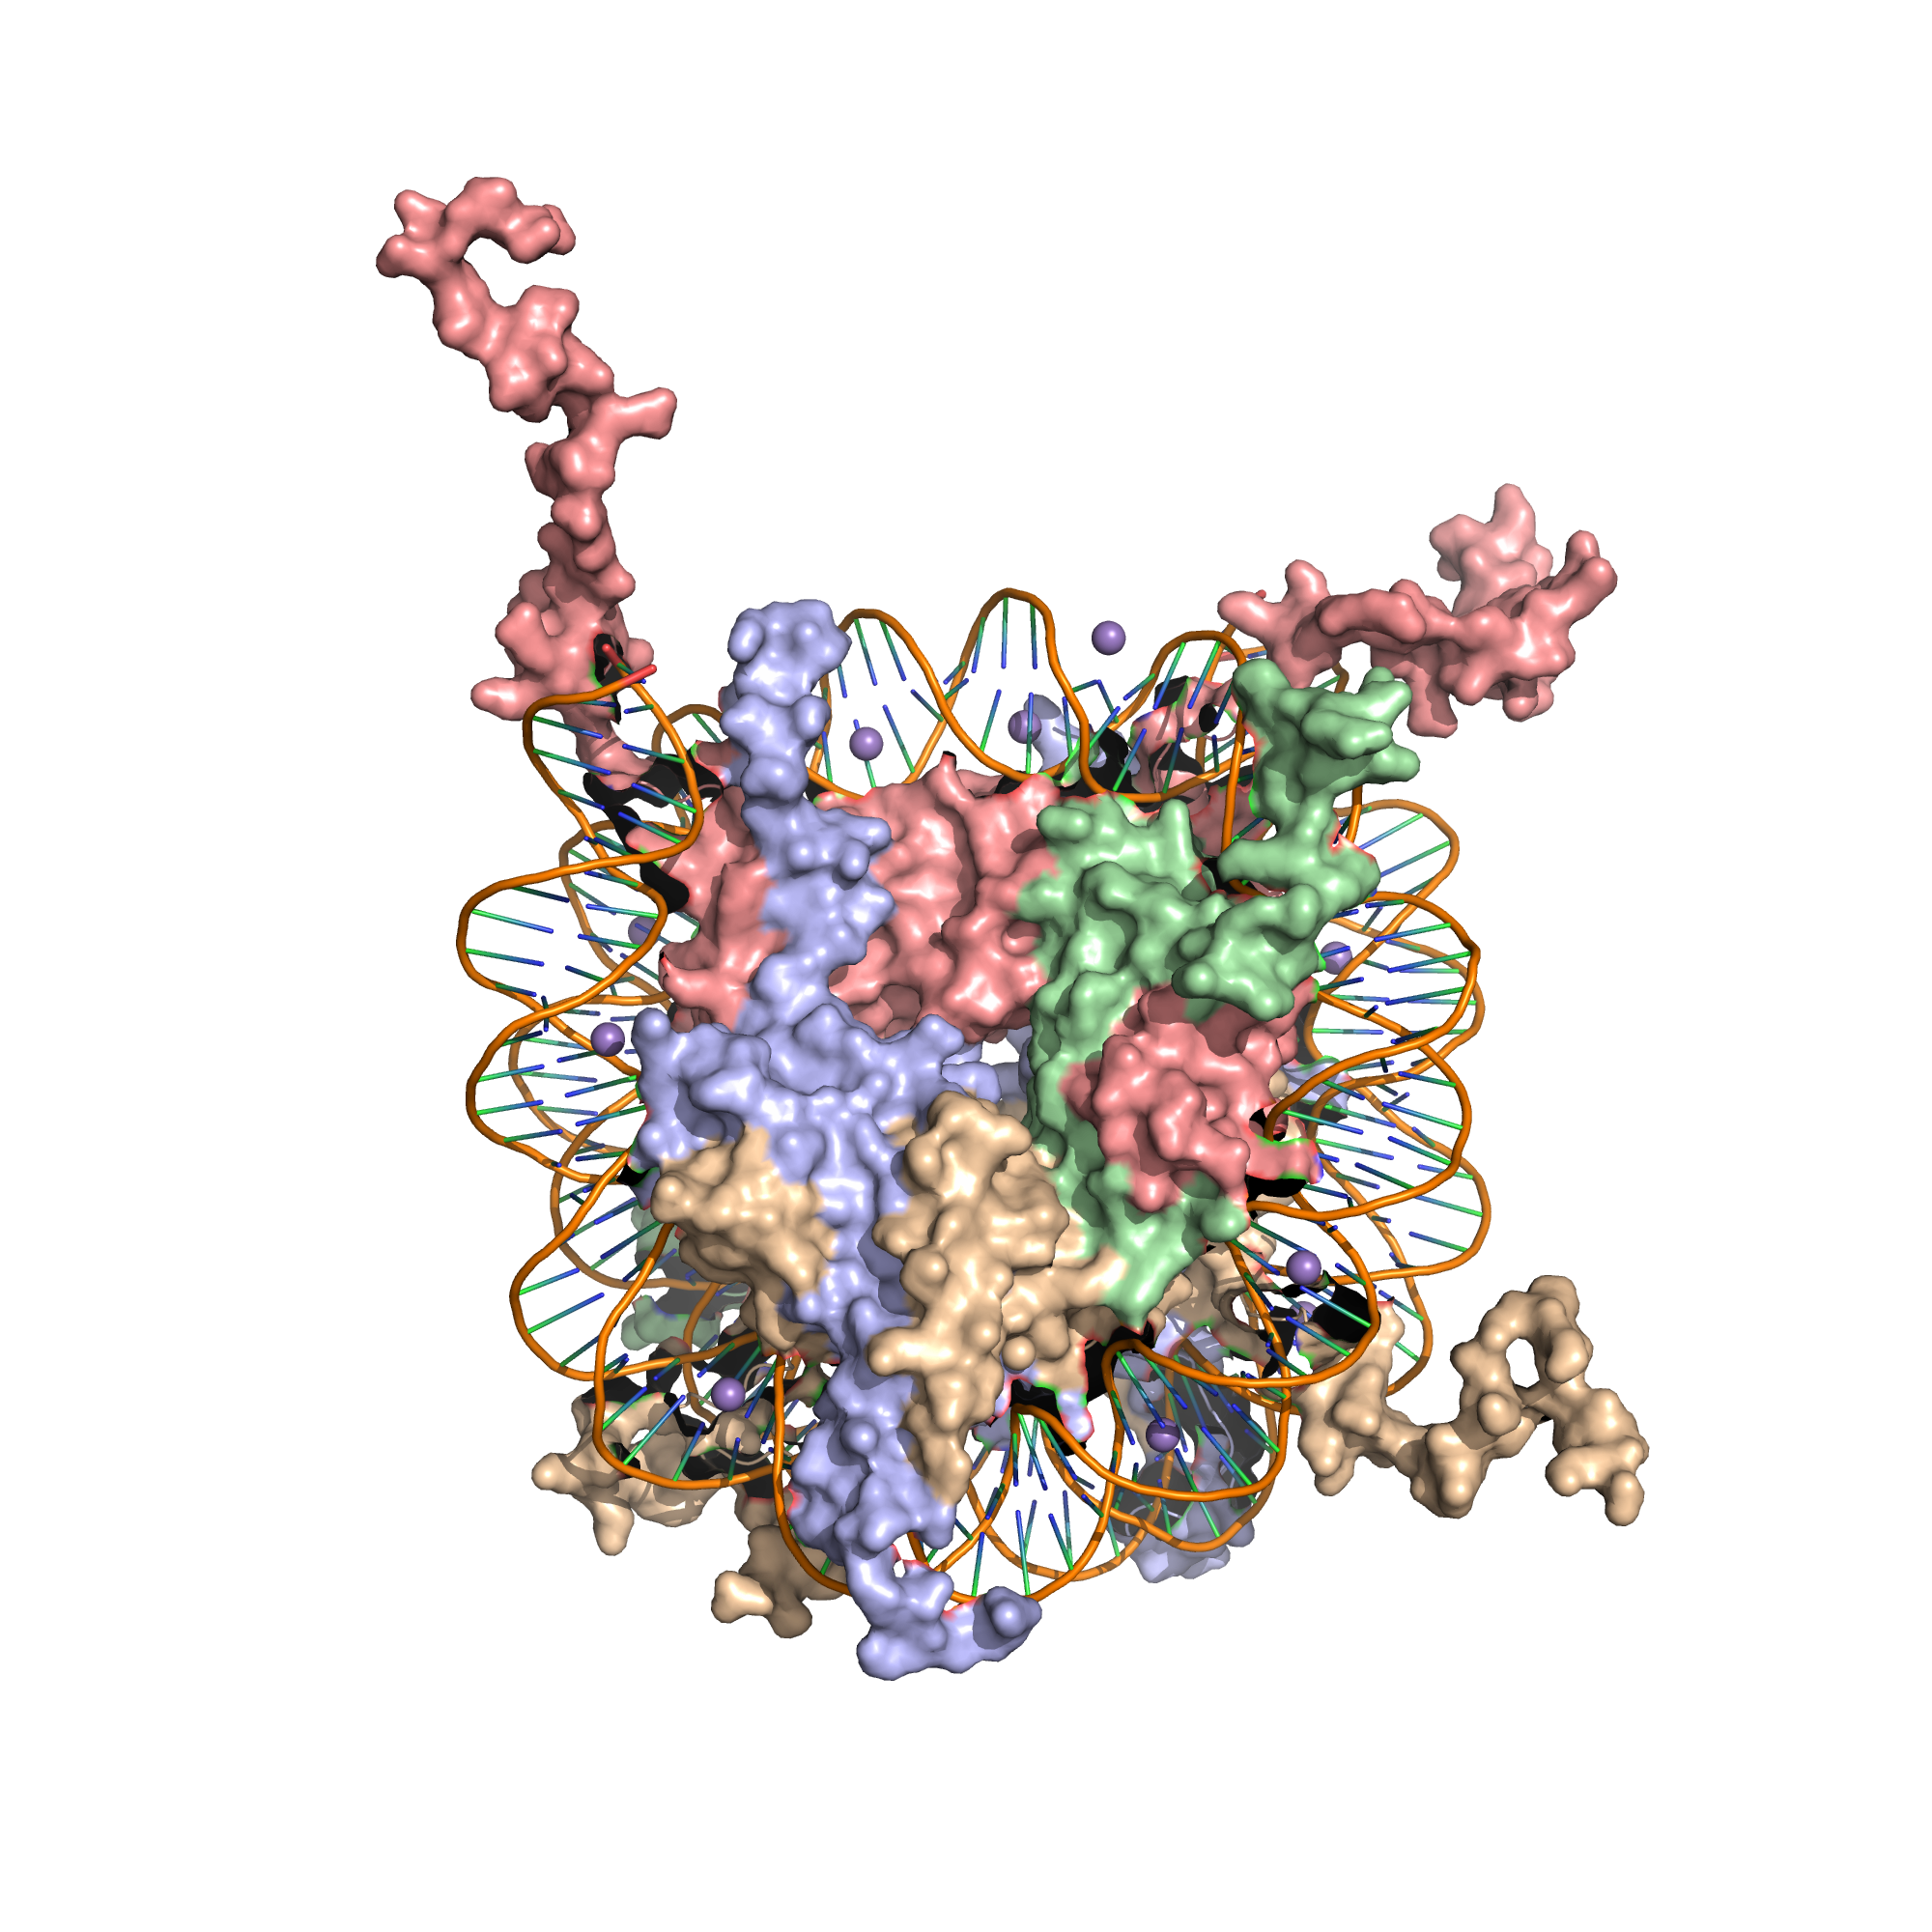
\includegraphics[width=0.7\linewidth]{./figures/dna/nucleosome_top} 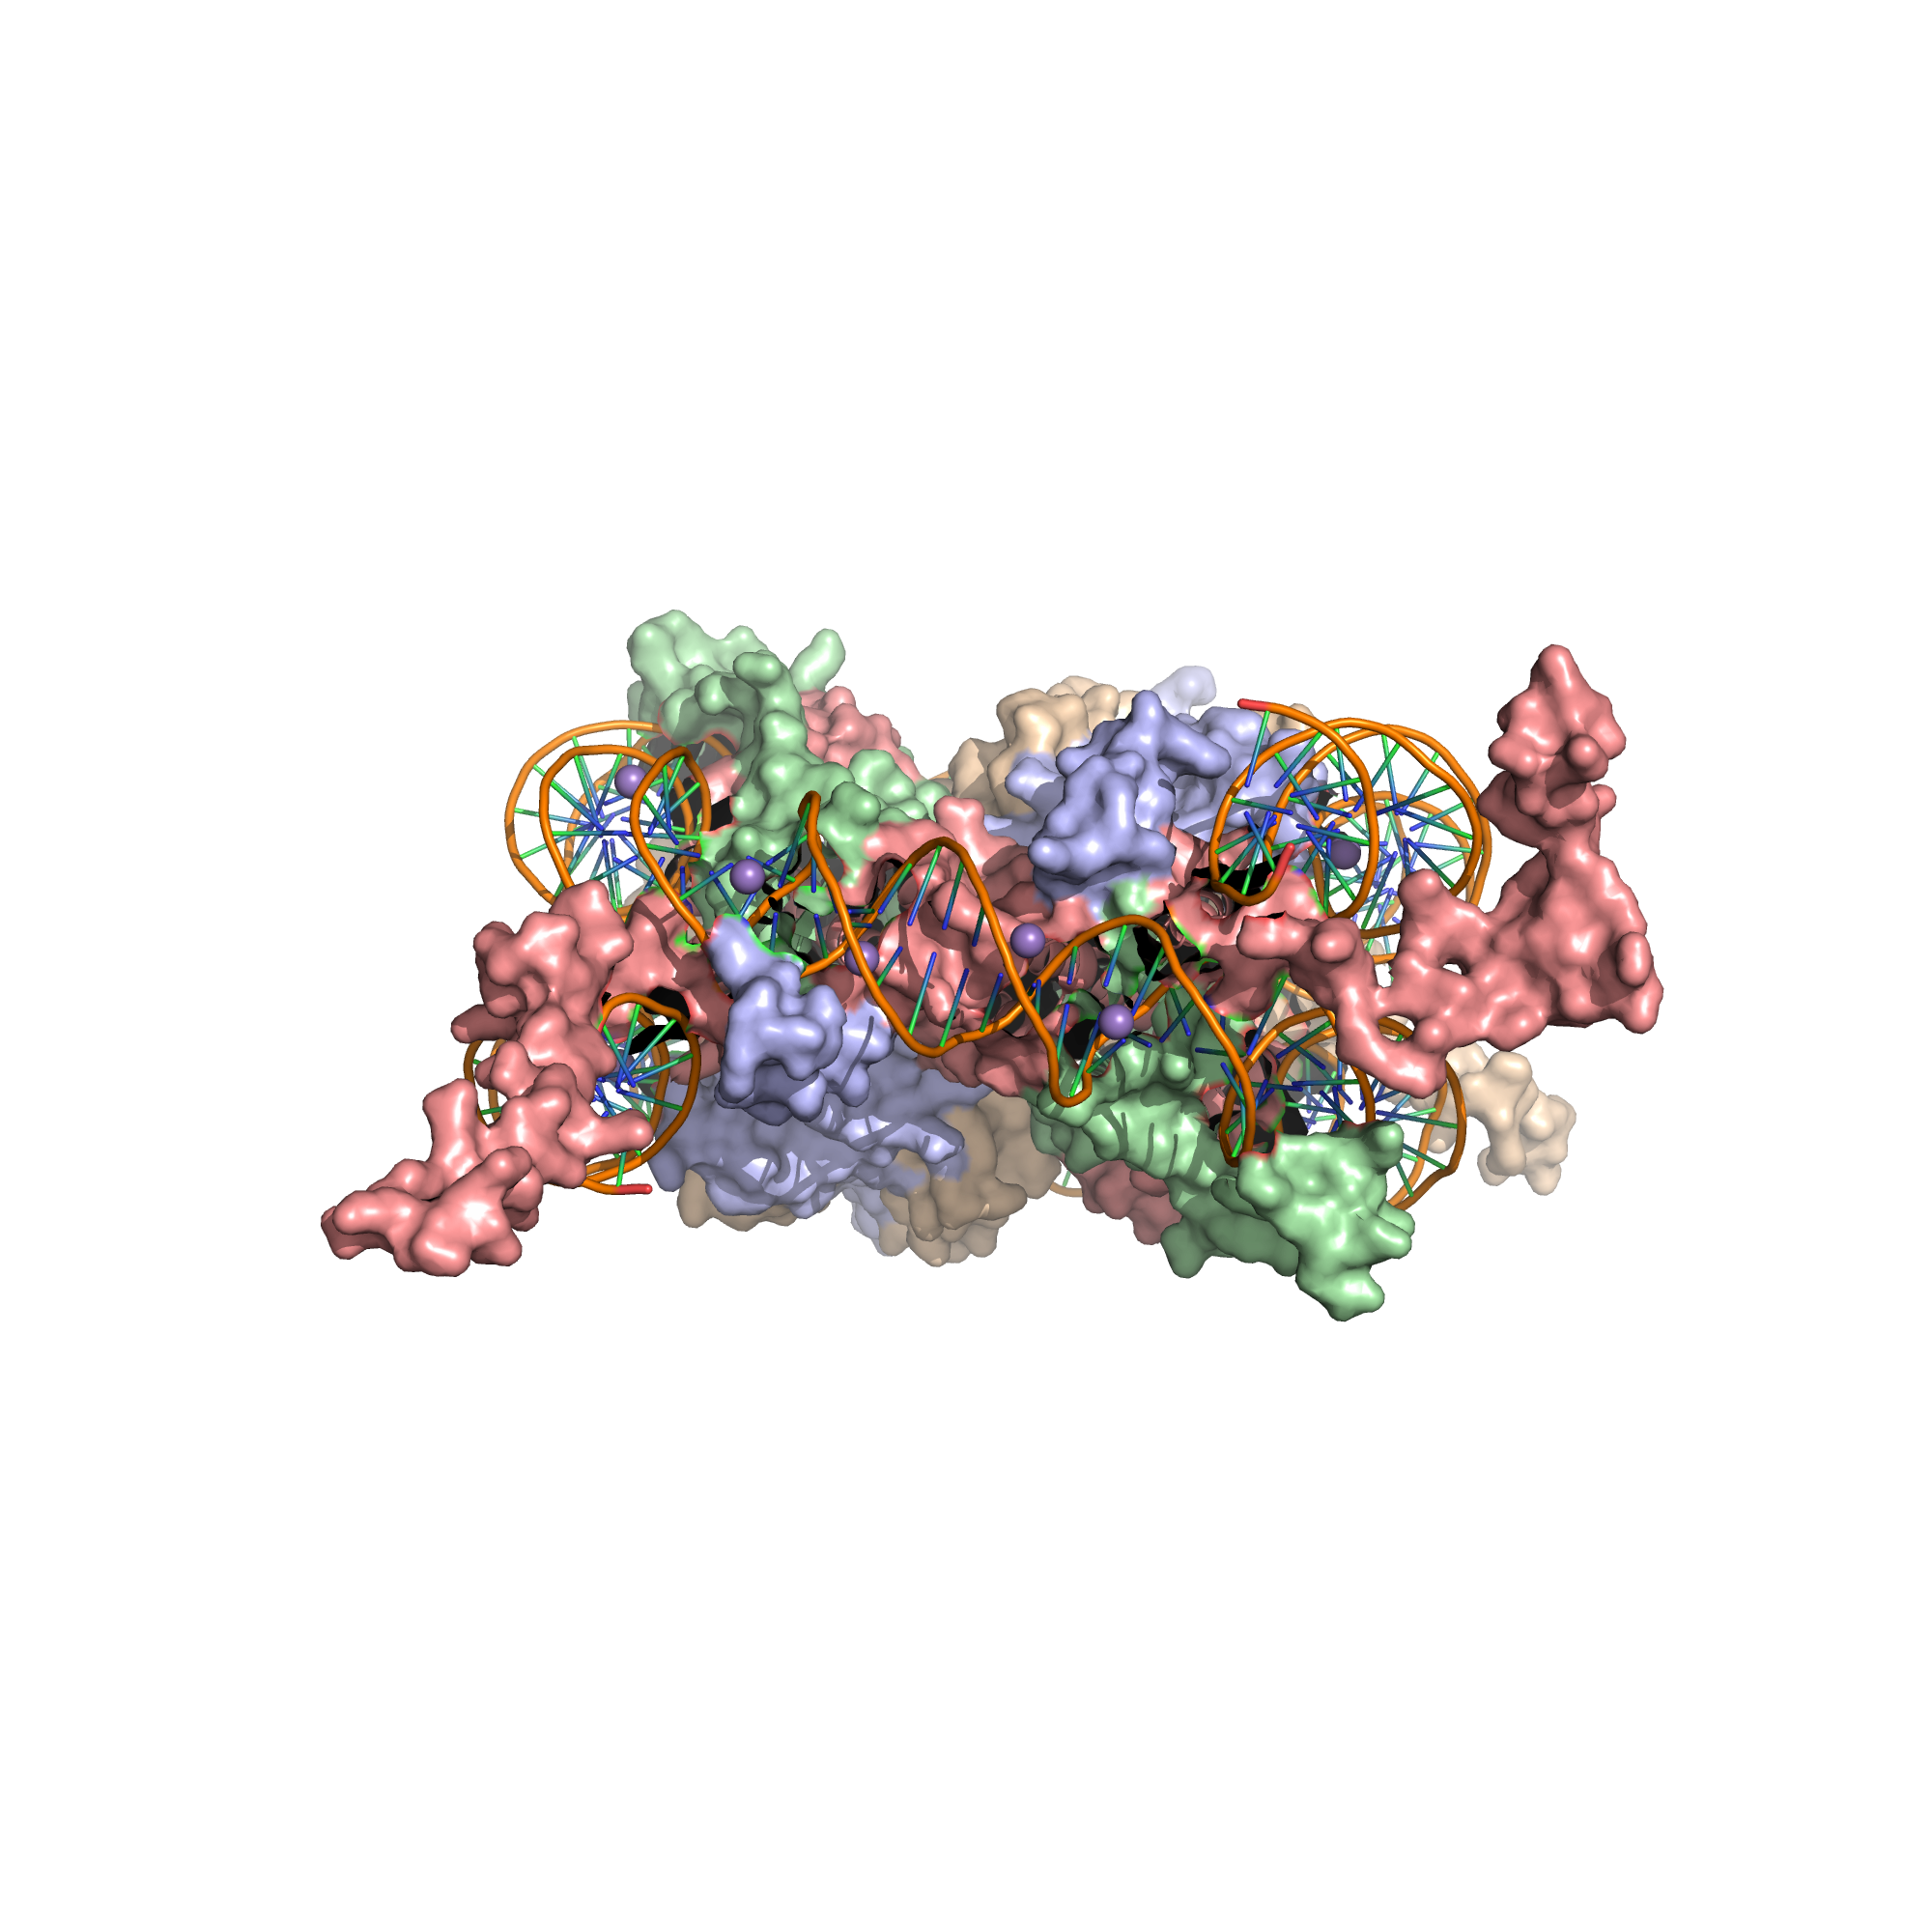
\includegraphics[width=0.7\linewidth]{./figures/dna/nucleosome_side} 

}

\caption{\href{https://www.rcsb.org/structure/1KX5}{X-Ray crystal structure of the nucleosome core particle consisting of H2A (lightblue), H2B (wheat), H3 (salmon) and H4 (palegreen) core histones, and DNA.tructure of the nucleosome core particle, NCP147, at 1.9 A resolution.} Top: view is from the top through the superhelical axis. Bottom: side view.}\label{fig:nucleosome}
\end{figure}

DNA must be compacted into nucleosomes to fit within the cell nucleus. In addition to nucleosome wrapping, eukaryotic chromatin is further compacted by being folded into a series of more complex structures, eventually forming a chromosome.

\href{https://commons.wikimedia.org/wiki/File:Chromatin_Structures.png}{The major structures in DNA compaction: DNA, the nucleosome, the 10 nm ``beads-on-a-string'' fibre, the 30 nm fibre and the metaphase chromosome.} \href{https://commons.wikimedia.org/wiki/File:Chromatin_Structures.png}{The major structures in DNA compaction: DNA, the nucleosome, the 10 nm ``beads-on-a-string'' fibre, the 30 nm fibre and the metaphase chromosome.}

\begin{figure}

{\centering 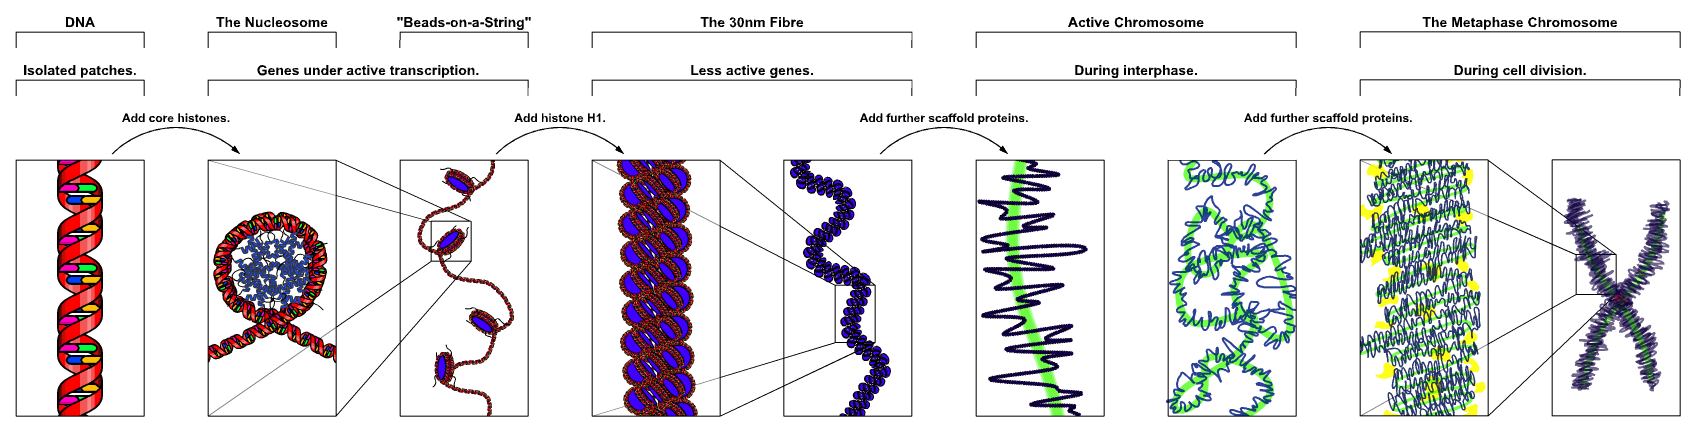
\includegraphics[width=0.7\linewidth]{./figures/chromosomes/Chromatin_Structures} 

}

\caption{\href{https://commons.wikimedia.org/wiki/File:Chromatin_Structures.png}{The major structures in DNA compaction: DNA, the nucleosome, the 10 nm ``beads-on-a-string'' fibre, the 30 nm fibre and the metaphase chromosome.}}\label{fig:structure}
\end{figure}

Nucleosomes are thought to carry epigenetically inherited information in the form of covalent modifications of their core histones. Nucleosome positions in the genome are not random, and it is important to know where each nucleosome is located because this determines the accessibility of the DNA to regulatory proteins.

Nucleosomes were first observed as particles in the electron microscope by Don and Ada Olins in 1974, and their existence and structure (as histone octamers surrounded by approximately 200 base pairs of DNA) were proposed by Roger Kornberg. The role of the nucleosome as a general gene repressor was demonstrated by Lorch et al.~in vitro, and by Han and Grunstein in vivo in 1987 and 1988, respectively.

The nucleosome core particle consists of approximately 146 base pairs (bp) of DNA wrapped in 1.67 left-handed superhelical turns around a histone octamer, consisting of 2 copies each of the core histones H2A, H2B, H3, and H4. Core particles are connected by stretches of linker DNA, which can be up to about 80 bp long. Technically, a nucleosome is defined as the core particle plus one of these linker regions; however the word is often synonymous with the core particle. Genome-wide nucleosome positioning maps are now available for many model organisms including mouse liver and brain.

Linker histones such as H1 and its isoforms are involved in chromatin compaction and sit at the base of the nucleosome near the DNA entry and exit binding to the linker region of the DNA. Non-condensed nucleosomes without the linker histone resemble ``beads on a string of DNA'' under an electron microscope.

Histones are subject to post translational modification by enzymes primarily on their N-terminal tails, but also in their globular domains.{[}14{]}{[}15{]} Such modifications include methylation, citrullination, acetylation, phosphorylation, SUMOylation, ubiquitination, and ADP-ribosylation. This affects their function of gene regulation.

In general, genes that are active have less bound histone, while inactive genes are highly associated with histones during interphase.{[}16{]} It also appears that the structure of histones has been evolutionarily conserved, as any deleterious mutations would be severely maladaptive. All histones have a highly positively charged N-terminus with many lysine and arginine residues.

In contrast to most eukaryotic cells, mature sperm cells largely use protamines to package their genomic DNA, most likely to achieve an even higher packaging ratio. Histone equivalents and a simplified chromatin structure have also been found in Archaea, suggesting that eukaryotes are not the only organisms that use nucleosomes.

\hypertarget{structure-1}{%
\section{Structure}\label{structure-1}}

\hypertarget{structure-of-the-core-particle}{%
\subsection{Structure of the core particle}\label{structure-of-the-core-particle}}

The nucleosome core particle (shown in Figure \ref{fig:nucleosome}) consists of about 146 base pair of DNA wrapped in 1.67 left-handed superhelical turns around the histone octamer, consisting of 2 copies each of the core histones H2A, H2B, H3, and H4. Adjacent nucleosomes are joined by a stretch of free DNA termed linker DNA (which varies from 10 - 80 bp in length depending on species and tissue type). The structures of over 20 different nucleosome core particles have been solved to date, including those containing histone variants and histones from different species. The structure of the nucleosome core particle is remarkably conserved, and even a change of over 100 residues between frog and yeast histones results in electron density maps with an overall root mean square deviation of only 1.6Å.

Nucleosome core particles are observed when chromatin in interphase is treated to cause the chromatin to unfold partially. The resulting image, via an electron microscope, is ``beads on a string''. The string is the DNA, while each bead in the nucleosome is a core particle. The nucleosome core particle is composed of DNA and histone proteins.

Partial DNAse digestion of chromatin reveals its nucleosome structure. Because DNA portions of nucleosome core particles are less accessible for DNAse than linking sections, DNA gets digested into fragments of lengths equal to multiplicity of distance between nucleosomes (180, 360, 540 base pairs etc.). Hence a very characteristic pattern similar to a ladder is visible during gel electrophoresis of that DNA. Such digestion can occur also under natural conditions during apoptosis (``cell suicide'' or programmed cell death), because autodestruction of DNA typically is its role.

\hypertarget{protein-interactions-within-the-nucleosome}{%
\subsection{Protein interactions within the nucleosome}\label{protein-interactions-within-the-nucleosome}}

The core histone proteins contains a characteristic structural motif termed the ``histone fold'', which consists of three alpha-helices (α1-3) separated by two loops (L1-2). In solution, the histones form H2A-H2B heterodimers and H3-H4 heterotetramers. Histones dimerise about their long α2 helices in an anti-parallel orientation, and, in the case of H3 and H4, two such dimers form a 4-helix bundle stabilised by extensive H3-H3' interaction. The H2A/H2B dimer binds onto the H3/H4 tetramer due to interactions between H4 and H2B, which include the formation of a hydrophobic cluster. The histone octamer is formed by a central H3/H4 tetramer sandwiched between two H2A/H2B dimers. Due to the highly basic charge of all four core histones, the histone octamer is stable only in the presence of DNA or very high salt concentrations.

\hypertarget{histone---dna-interactions}{%
\section{Histone - DNA interactions}\label{histone---dna-interactions}}

The nucleosome contains over 120 direct protein-DNA interactions and several hundred water-mediated ones. In all, histones make five types of interactions with DNA:

\begin{itemize}
\tightlist
\item
  Helix-dipoles form alpha-helixes in H2B, H3, and H4 cause a net positive charge to accumulate at the point of interaction with negatively charged phosphate groups on DNA
\item
  Hydrogen bonds between the DNA backbone and the amide group on the main chain of histone proteins
\item
  Nonpolar interactions between the histone and deoxyribose sugars on DNA
\item
  Salt bridges and hydrogen bonds between side chains of basic amino acids (especially lysine and arginine) and phosphate oxygens on DNA
\item
  Non-specific minor groove insertions of the H3 and H2B N-terminal tails into two minor grooves each on the DNA molecule
  The highly basic nature of histones, aside from facilitating DNA-histone interactions, contributes to their water solubility.
\end{itemize}

\hypertarget{higher-order-structure-of-dna}{%
\section{Higher order structure of DNA}\label{higher-order-structure-of-dna}}

The organization of the DNA that is achieved by the nucleosome cannot fully explain the packaging of DNA observed in the cell nucleus. Further compaction of chromatin into the cell nucleus is necessary, but is not yet well understood. The current understanding is that repeating nucleosomes with intervening ``linker'' DNA form a 10-nm-fiber, described as ``beads on a string'', and have a packing ratio of about five to ten. A chain of nucleosomes can be arranged in a 30 nm fiber, a compacted structure with a packing ratio of \textasciitilde{}50 and whose formation is dependent on the presence of the H1 histone.

A crystal structure of a tetranucleosome has been presented and used to build up a proposed structure of the 30 nm fiber as a two-start helix. There is still a certain amount of contention regarding this model, as it is incompatible with recent electron microscopy data. Beyond this, the structure of chromatin is poorly understood, but it is classically suggested that the 30 nm fiber is arranged into loops along a central protein scaffold to form transcriptionally active euchromatin. Further compaction leads to transcriptionally inactive heterochromatin.

\hypertarget{dynamics}{%
\section{Dynamics}\label{dynamics}}

Although the nucleosome is a very stable protein-DNA complex, it is not static and has been shown to undergo a number of different structural re-arrangements including nucleosome sliding and DNA site exposure. Depending on the context, nucleosomes can inhibit or facilitate transcription factor binding. Nucleosome positions are controlled by three major contributions: First, the intrinsic binding affinity of the histone octamer depends on the DNA sequence. Second, the nucleosome can be displaced or recruited by the competitive or cooperative binding of other protein factors. Third, the nucleosome may be actively translocated by ATP-dependent remodeling complexes.

\hypertarget{nucleosome-free-region}{%
\section{Nucleosome free region}\label{nucleosome-free-region}}

Promoters of active genes have nucleosome free regions (NFR). This allows for promoter DNA accessibility to various proteins, such as transcription factors. Nucleosome free region typically spans for 200 nucleotides in S. cerevisae Well-positioned nucleosomes form boundaries of NFR. These nucleosomes are called +1-nucleosome and −1-nucleosome and are located at canonical distances downstream and upstream, respectively, from transcription start site. +1-nucleosome and several downstream nucleosomes also tend to incorporate H2A.Z histone variant.

\hypertarget{modulating-nucleosome-structure}{%
\section{Modulating nucleosome structure}\label{modulating-nucleosome-structure}}

Eukaryotic genomes are ubiquitously associated into chromatin; however, cells must spatially and temporally regulate specific loci independently of bulk chromatin. In order to achieve the high level of control required to co-ordinate nuclear processes such as DNA replication, repair, and transcription, cells have developed a variety of means to locally and specifically modulate chromatin structure and function. This can involve covalent modification of histones, the incorporation of histone variants, and non-covalent remodelling by ATP-dependent remodeling enzymes.

\hypertarget{histone-post-translational-modifications}{%
\section{Histone post-translational modifications}\label{histone-post-translational-modifications}}

Since they were discovered in the mid-1960s, histone modifications have been predicted to affect transcription. The fact that most of the early post-translational modifications found were concentrated within the tail extensions that protrude from the nucleosome core lead to two main theories regarding the mechanism of histone modification. The first of the theories suggested that they may affect electrostatic interactions between the histone tails and DNA to ``loosen'' chromatin structure. Later it was proposed that combinations of these modifications may create binding epitopes with which to recruit other proteins. Recently, given that more modifications have been found in the structured regions of histones, it has been put forward that these modifications may affect histone-DNA and histone-histone interactions within the nucleosome core. Modifications (such as acetylation or phosphorylation) that lower the charge of the globular histone core are predicted to ``loosen'' core-DNA association; the strength of the effect depends on location of the modification within the core. Some modifications have been shown to be correlated with gene silencing; others seem to be correlated with gene activation. Common modifications include acetylation, methylation, or ubiquitination of lysine; methylation of arginine; and phosphorylation of serine. The information stored in this way is considered epigenetic, since it is not encoded in the DNA but is still inherited to daughter cells. The maintenance of a repressed or activated status of a gene is often necessary for cellular differentiation.

\hypertarget{dynamic-nucleosome-remodelling-across-the-yeast-genome}{%
\section{Dynamic nucleosome remodelling across the yeast genome}\label{dynamic-nucleosome-remodelling-across-the-yeast-genome}}

Studies in 2007 have catalogued nucleosome positions in yeast and shown that nucleosomes are depleted in promoter regions and origins of replication. About 80\% of the yeast genome appears to be covered by nucleosomes and the pattern of nucleosome positioning clearly relates to DNA regions that regulate transcription, regions that are transcribed and regions that initiate DNA replication. Most recently, a new study examined dynamic changes in nucleosome repositioning during a global transcriptional reprogramming event to elucidate the effects on nucleosome displacement during genome-wide transcriptional changes in yeast (Saccharomyces cerevisiae). The results suggested that nucleosomes that were localized to promoter regions are displaced in response to stress (like heat shock). In addition, the removal of nucleosomes usually corresponded to transcriptional activation and the replacement of nucleosomes usually corresponded to transcriptional repression, presumably because transcription factor binding sites became more or less accessible, respectively. In general, only one or two nucleosomes were repositioned at the promoter to effect these transcriptional changes. However, even in chromosomal regions that were not associated with transcriptional changes, nucleosome repositioning was observed, suggesting that the covering and uncovering of transcriptional DNA does not necessarily produce a transcriptional event. After transcription, the rDNA region has to protected from any damage, it suggested HMGB proteins play a major role in protecting the nucleosome free region.

\hypertarget{histones}{%
\section{Histones}\label{histones}}

Five major families of histones exist: H1/H5, H2A, H2B, H3, and H4. Histones H2A, H2B, H3 and H4 are known as the core histones, while histones H1/H5 are known as the linker histones.

Histones are subdivided into canonical replication-dependent histones that are expressed during the S-phase of cell cycle and replication-independent histone variants, expressed during the whole cell cycle. In animals, genes encoding canonical histones are typically clustered along the chromosome, lack introns and use a stem loop structure at the 3' end instead of a polyA tail. Genes encoding histone variants are usually not clustered, have introns and their mRNAs are regulated with polyA tails. Complex multicellular organisms typically have a higher number of histone variants providing a variety of different functions. Recent data are accumulating about the roles of diverse histone variants highlighting the functional links between variants and the delicate regulation of organism development. Histone variants from different organisms, their classification and variant specific features can be found in ``HistoneDB 2.0 - Variants'' database.

Histones were discovered in 1884 by Albrecht Kossel. The word ``histone'' dates from the late 19th century and is derived from the German word ``Histon'', a word itself of uncertain origin.

In the 1960s, Vincent Allfrey and Alfred Mirsky had suggested, based on their analyses of histones, that acetylation and methylation of histones could provide a transcriptional control mechanism, but did not have available the kind of detailed analysis that later investigators were able to conduct to show how such regulation could be gene-specific. Until the early 1990s, histones were dismissed by most as inert packing material for eukaryotic nuclear DNA, a view based in part on the models of Mark Ptashne and others, who believed that transcription was activated by protein-DNA and protein-protein interactions on largely naked DNA templates, as is the case in bacteria.

During the 1980s, Yahli Lorch and Roger Kornberg showed that a nucleosome on a core promoter prevents the initiation of transcription in vitro, and Michael Grunstein demonstrated that histones repress transcription in vivo, leading to the idea of the nucleosome as a general gene repressor. Relief from repression is believed to involve both histone modification and the action of chromatin-remodeling complexes. Vincent Allfrey and Alfred Mirsky had earlier proposed a role of histone modification in transcriptional activation, regarded as a molecular manifestation of epigenetics. Michael Grunstein and David Allis found support for this proposal, in the importance of histone acetylation for transcription in yeast and the activity of the transcriptional activator Gcn5 as a histone acetyltransferase.

Histones are found in the nuclei of eukaryotic cells, and in certain Archaea, namely Proteoarchaea and Euryarchaea, but not in bacteria. The unicellular algae known as dinoflagellates were previously thought to be the only eukaryotes that completely lack histones, however, later studies showed that their DNA still encodes histone genes. Unlike the core histones, lysine-rich linker histone (H1) proteins are found in bacteria, otherwise known as nucleoprotein HC1/HC2.

Archaeal histones may well resemble the evolutionary precursors to eukaryotic histones. Histone proteins are among the most highly conserved proteins in eukaryotes, emphasizing their important role in the biology of the nucleus.:939 In contrast mature sperm cells largely use protamines to package their genomic DNA, most likely because this allows them to achieve an even higher packaging ratio.

Histones are believed to have evolved from ribosomal proteins with which they share much in common, both being short and basic proteins.

Histones undergo posttranslational modifications that alter their interaction with DNA and nuclear proteins. The H3 and H4 histones have long tails protruding from the nucleosome, which can be covalently modified at several places. Modifications of the tail include methylation, acetylation, phosphorylation, ubiquitination, SUMOylation, citrullination, and ADP-ribosylation. The core of the histones H2A and H2B can also be modified. Combinations of modifications are thought to constitute a code, the so-called ``histone code''. Histone modifications act in diverse biological processes such as gene regulation, DNA repair, chromosome condensation (mitosis) and spermatogenesis (meiosis).

The common nomenclature of histone modifications is:

\begin{itemize}
\tightlist
\item
  The name of the histone (e.g., H3)
\item
  The single-letter amino acid abbreviation (e.g., K for Lysine) and the amino acid position in the protein
\item
  The type of modification (Me: methyl, P: phosphate, Ac: acetyl, Ub: ubiquitin)
\item
  The number of modifications (only Me is known to occur in more than one copy per residue. 1, 2 or 3 is mono-, di- or tri-methylation)
\end{itemize}

So H3K4me1 denotes the monomethylation of the 4th residue (a lysine) from the start (i.e., the N-terminal) of the H3 protein.

\hypertarget{functions-of-histone-modifications}{%
\section{Functions of histone modifications}\label{functions-of-histone-modifications}}

A huge catalogue of histone modifications have been described, but a functional understanding of most is still lacking. Collectively, it is thought that histone modifications may underlie a histone code, whereby combinations of histone modifications have specific meanings. However, most functional data concerns individual prominent histone modifications that are biochemically amenable to detailed study.

\hypertarget{chemistry-of-histone-modifications}{%
\section{Chemistry of histone modifications}\label{chemistry-of-histone-modifications}}

\hypertarget{lysine-methylation}{%
\subsection{Lysine methylation}\label{lysine-methylation}}

The addition of one, two, or many methyl groups to lysine has little effect on the chemistry of the histone; methylation leaves the charge of the lysine intact and adds a minimal number of atoms so steric interactions are mostly unaffected. However, proteins containing Tudor, chromo or PHD domains, amongst others, can recognise lysine methylation with exquisite sensitivity and differentiate mono, di and tri-methyl lysine, to the extent that, for some lysines (e.g.: H4K20) mono, di and tri-methylation appear to have different meanings. Because of this, lysine methylation tends to be a very informative mark and dominates the known histone modification functions.

\hypertarget{arginine-methylation}{%
\subsection{Arginine methylation}\label{arginine-methylation}}

Enzymes called peptidylarginine deiminases (PADs) hydrolyze the imine group of arginines and attach a keto group, so that there is one less positive charge on the amino acid residue. This process has been involved in the activation of gene expression by making the modified histones less tightly bound to DNA and thus making the chromatin more accessible. PADs can also produce the opposite effect by removing or inhibiting mono-methylation of arginine residues on histones and thus antagonizing the positive effect arginine methylation has on transcriptional activity.

\hypertarget{lysine-acetylation}{%
\subsection{Lysine acetylation}\label{lysine-acetylation}}

Addition of an acetyl group has a major chemical effect on lysine as it neutralises the positive charge. This reduces electrostatic attraction between the histone and the negatively charged DNA backbone, loosening the chromatin structure; highly acetylated histones form more accessible chromatin and tend to be associated with active transcription. Lysine acetylation appears to be less precise in meaning than methylation, in that histone acetyltransferases tend to act on more than one lysine; presumably this reflects the need to alter multiple lysines to have a significant effect on chromatin structure. The modification includes H3K27ac.

\hypertarget{serinethreoninetyrosine-phosphorylation}{%
\subsection{Serine/threonine/tyrosine phosphorylation}\label{serinethreoninetyrosine-phosphorylation}}

Addition of a negatively charged phosphate group can lead to major changes in protein structure, leading to the well-characterised role of phosphorylation in controlling protein function. It is not clear what structural implications histone phosphorylation has, but histone phosphorylation has clear functions as a post-translational modification, and binding domains such as BRCT have been characterised.

\hypertarget{functions-in-transcription}{%
\section{Functions in transcription}\label{functions-in-transcription}}

Most well-studied histone modifications are involved in control of transcription.

Two histone modifications are particularly associated with active transcription:

\hypertarget{trimethylation-of-h3-lysine-4-h3k4me3}{%
\subsection{Trimethylation of H3 lysine 4 (H3K4me3)}\label{trimethylation-of-h3-lysine-4-h3k4me3}}

This trimethylation occurs at the promoter of active genes and is performed by the COMPASS complex. Despite the conservation of this complex and histone modification from yeast to mammals, it is not entirely clear what role this modification plays. However, it is an excellent mark of active promoters and the level of this histone modification at a gene's promoter is broadly correlated with transcriptional activity of the gene. The formation of this mark is tied to transcription in a rather convoluted manner: early in transcription of a gene, RNA polymerase II undergoes a switch from initiating' to `elongating', marked by a change in the phosphorylation states of the RNA polymerase II C terminal domain (CTD). The same enzyme that phosphorylates the CTD also phosphorylates the Rad6 complex, which in turn adds a ubiquitin mark to H2B K123 (K120 in mammals). H2BK123Ub occurs throughout transcribed regions, but this mark is required for COMPASS to trimethylate H3K4 at promoters.
Trimethylation of H3 lysine 36 (H3K36me3)
This trimethylation occurs in the body of active genes and is deposited by the methyltransferase Set2. This protein associates with elongating RNA polymerase II, and H3K36Me3 is indicative of actively transcribed genes. H3K36Me3 is recognised by the Rpd3 histone deacetylase complex, which removes acetyl modifications from surrounding histones, increasing chromatin compaction and repressing spurious transcription. Increased chromatin compaction prevents transcription factors from accessing DNA, and reduces the likelihood of new transcription events being initiated within the body of the gene. This process therefore helps ensure that transcription is not interrupted.

Three histone modifications are particularly associated with repressed genes:

\hypertarget{trimethylation-of-h3-lysine-27-h3k27me3}{%
\subsection{Trimethylation of H3 lysine 27 (H3K27me3)}\label{trimethylation-of-h3-lysine-27-h3k27me3}}

This histone modification is depositied by the polycomb complex PRC2. It is a clear marker of gene repression, and is likely bound by other proteins to exert a repressive function. Another polycomb complex, PRC1, can bind H3K27me3 and adds the histone modification H2AK119Ub which aids chromatin compaction. Based on this data it appears that PRC1 is recruited through the action of PRC2, however, recent studies show that PRC1 is recruited to the same sites in the absence of PRC2.
Di and tri-methylation of H3 lysine 9 (H3K9me2/3)
H3K9me2/3 is a well-characterised marker for heterochromatin, and is therefore strongly associated with gene repression. The formation of heterochromatin has been best studied in the yeast Schizosaccharomyces pombe, where it is initiated by recruitment of the RNA-induced transcriptional silencing (RITS) complex to double stranded RNAs produced from centromeric repeats. RITS recruits the Clr4 histone methyltransferase which deposits H3K9me2/3. This process is called histone methylation. H3K9Me2/3 serves as a binding site for the recruitment of Swi6 (heterochromatin protein 1 or HP1, another classic heterochromatin marker) which in turn recruits further repressive activities including histone modifiers such as histone deacetylases and histone methyltransferases.
Trimethylation of H4 lysine 20 (H4K20me3)
This modification is tightly associated with heterochromatin, although its functional importance remains unclear. This mark is placed by the Suv4-20h methyltransferase, which is at least in part recruited by heterochromatin protein 1.
Bivalent promoters
Analysis of histone modifications in embryonic stem cells (and other stem cells) revealed many gene promoters carrying both H3K4Me3 and H3K27Me3, in other words these promoters display both activating and repressing marks simultaneously. This peculiar combination of modifications marks genes that are poised for transcription; they are not required in stem cells, but are rapidly required after differentiation into some lineages. Once the cell starts to differentiate, these bivalent promoters are resolved to either active or repressive states depending on the chosen lineage.

Marking sites of DNA damage is an important function for histone modifications. It also protects DNA from getting destroyed by ultraviolet radiation of sun.

\hypertarget{chromosome-condensation}{%
\subsection{Chromosome condensation}\label{chromosome-condensation}}

Phosphorylation of H3 at serine 10 (phospho-H3S10)
The mitotic kinase aurora B phosphorylates histone H3 at serine 10, triggering a cascade of changes that mediate mitotic chromosome condensation. Condensed chromosomes therefore stain very strongly for this mark, but H3S10 phosphorylation is also present at certain chromosome sites outside mitosis, for example in pericentric heterochromatin of cells during G2. H3S10 phosphorylation has also been linked to DNA damage caused by R-loop formation at highly transcribed sites.
Phosphorylation H2B at serine 10/14 (phospho-H2BS10/14)
Phosphorylation of H2B at serine 10 (yeast) or serine 14 (mammals) is also linked to chromatin condensation, but for the very different purpose of mediating chromosome condensation during apoptosis. This mark is not simply a late acting bystander in apoptosis as yeast carrying mutations of this residue are resistant to hydrogen peroxide-induced apoptotic cell death.



\chapter{DNA replication}\label{dna-replication}

In molecular biology, DNA replication is the biological process of producing two identical replicas of DNA from one original DNA molecule. DNA replication occurs in all living organisms acting as the basis for biological inheritance. The cell possesses the distinctive property of division, which makes replication of DNA essential.

DNA is made up of a double helix of two complementary strands. During replication, these strands are separated. Each strand of the original DNA molecule then serves as a template for the production of its counterpart, a process referred to as semiconservative replication. As a result of semi-conservative replication, the new helix will be composed of an original DNA strand as well as a newly synthesized strand. Cellular proofreading and error-checking mechanisms ensure near perfect fidelity for DNA replication.



\begin{figure}

{\centering 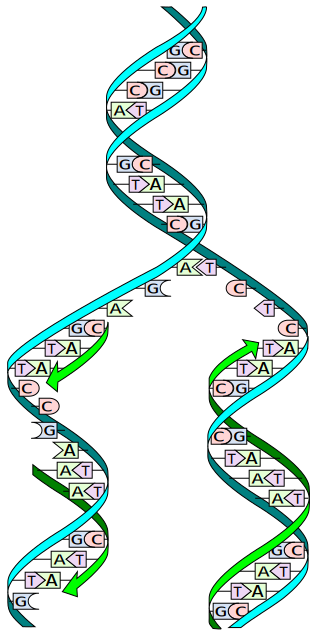
\includegraphics[width=0.7\linewidth]{./figures/replication/DNA_replication_split} 

}

\caption{\href{https://commons.wikimedia.org/wiki/File:DNA_replication_split.svg}{DNA polymerases adds nucleotides to the 3′ end of a strand of DNA. If a mismatch is accidentally incorporated, the polymerase is inhibited from further extension. Proofreading removes the mismatched nucleotide and extension continues.}}\label{fig:repfork}
\end{figure}

In a cell, DNA replication begins at specific locations, or origins of replication, in the genome. Unwinding of DNA at the origin and synthesis of new strands, accommodated by an enzyme known as helicase, results in replication forks growing bi-directionally from the origin. A number of proteins are associated with the replication fork to help in the initiation and continuation of DNA synthesis. Most prominently, DNA polymerase synthesizes the new strands by adding nucleotides that complement each (template) strand. DNA replication occurs during the S-stage of interphase.

DNA replication (DNA amplification) can also be performed in vitro (artificially, outside a cell). DNA polymerases isolated from cells and artificial DNA primers can be used to start DNA synthesis at known sequences in a template DNA molecule. Polymerase chain reaction (PCR), ligase chain reaction (LCR), and transcription-mediated amplification (TMA) are examples.

\hypertarget{eukaryotic-dna-replication}{%
\section{Eukaryotic DNA replication}\label{eukaryotic-dna-replication}}

Eukaryotic DNA replication is a conserved mechanism that restricts DNA replication to once per cell cycle. Eukaryotic DNA replication of chromosomal DNA is central for the duplication of a cell and is necessary for the maintenance of the eukaryotic genome.

DNA replication is the action of DNA polymerases synthesizing a DNA strand complementary to the original template strand. To synthesize DNA, the double-stranded DNA is unwound by DNA helicases ahead of polymerases, forming a replication fork containing two single-stranded templates. Replication processes permit the copying of a single DNA double helix into two DNA helices, which are divided into the daughter cells at mitosis. The major enzymatic functions carried out at the replication fork are well conserved from prokaryotes to eukaryotes, but the replication machinery in eukaryotic DNA replication is a much larger complex, coordinating many proteins at the site of replication, forming the replisome.

After the replicative helicase has unwound the parental DNA duplex, exposing two single-stranded DNA templates, replicative polymerases are needed to generate two copies of the parental genome. DNA polymerase function is highly specialized and accomplish replication on specific templates and in narrow localizations. At the eukaryotic replication fork, there are three distinct replicative polymerase complexes that contribute to DNA replication: Polymerase α, Polymerase δ, and Polymerase ε. These three polymerases are essential for viability of the cell.



\begin{figure}

{\centering 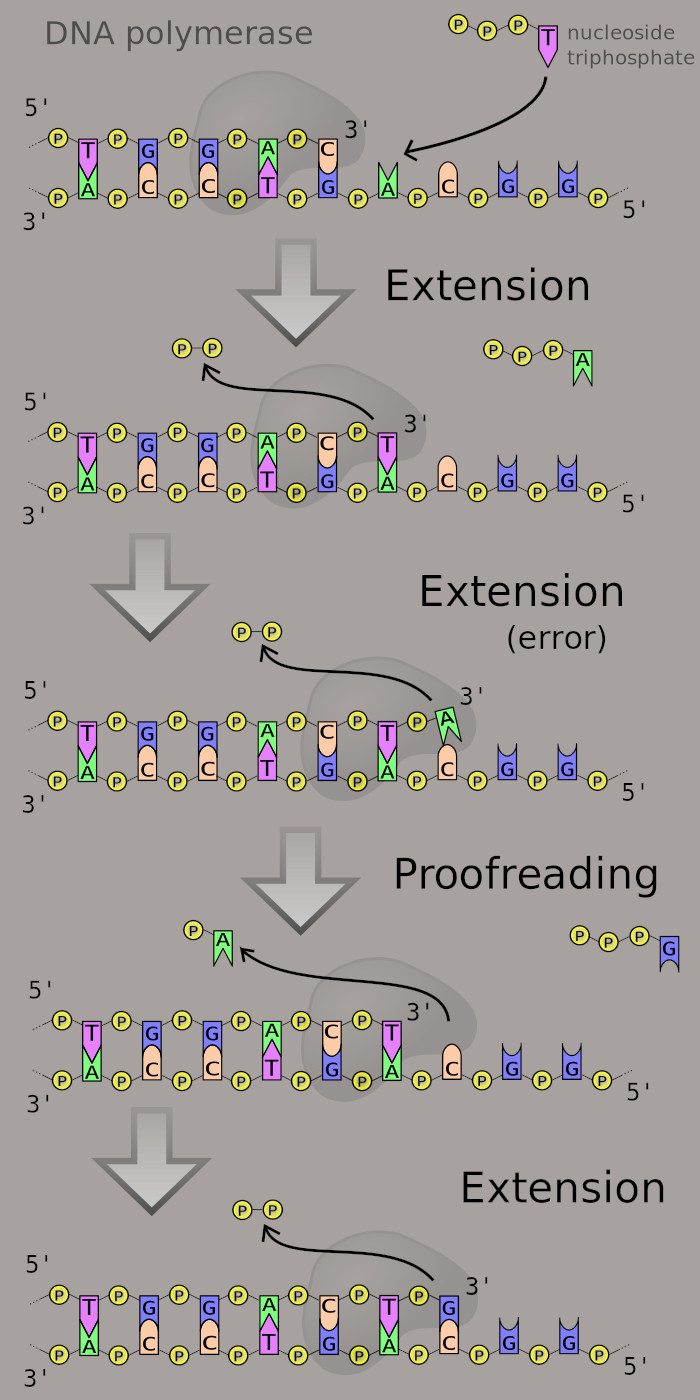
\includegraphics[width=0.7\linewidth]{./figures/replication/DNA_polymerase} 

}

\caption{\href{https://commons.wikimedia.org/wiki/File:DNA_polymerase.svg}{DNA polymerases adds nucleotides to the 3′ end of a strand of DNA. If a mismatch is accidentally incorporated, the polymerase is inhibited from further extension. Proofreading removes the mismatched nucleotide and extension continues.}}\label{fig:polymerase}
\end{figure}

Because DNA polymerases require a primer on which to begin DNA synthess, polymerase α (Pol α) acts as a replicative primase. Pol α is associated with an RNA primase and this complex accomplishes the priming task by synthesizing a primer that contains a short 10 nucleotide stretch of RNA followed by 10 to 20 DNA bases. Importantly, this priming action occurs at replication initiation at origins to begin leading-strand synthesis and also at the 5' end of each Okazaki fragment on the lagging strand.

However, Pol α is not able to continue DNA replication and must be replaced with another polymerase to continue DNA synthesis. Polymerase switching requires clamp loaders and it has been proven that normal DNA replication requires the coordinated actions of all three DNA polymerases: Pol α for priming synthesis, Pol ε for leading-strand replication, and the Pol δ, which is constantly loaded, for generating Okazaki fragments during lagging-strand synthesis.

\begin{itemize}
\tightlist
\item
  Polymerase α (Pol α): Forms a complex with a small catalytic subunit (PriS) and a large noncatalytic (PriL) subunit. First, synthesis of an RNA primer allows DNA synthesis by DNA polymerase alpha. Occurs once at the origin on the leading strand and at the start of each Okazaki fragment on the lagging strand. Pri subunits act as a primase, synthesizing an RNA primer. DNA Pol α elongates the newly formed primer with DNA nucleotides. After around 20 nucleotides, elongation is taken over by Pol ε on the leading strand and Pol δ on the lagging strand.
\item
  Polymerase δ (Pol δ): Highly processive and has proofreading, 3'-\textgreater{}5' exonuclease activity. In vivo, it is the main polymerase involved in both lagging strand and leading strand synthesis.
\item
  Polymerase ε (Pol ε): Highly processive and has proofreading, 3'-\textgreater{}5' exonuclease activity. Highly related to pol δ, in vivo it functions mainly in error checking of pol δ.
\end{itemize}

The replisome is responsible for copying the entirety of genomic DNA in each proliferative cell. This process allows for the high-fidelity passage of hereditary/genetic information from parental cell to daughter cell and is thus essential to all organisms. Much of the cell cycle is built around ensuring that DNA replication occurs without errors.



\begin{figure}

{\centering 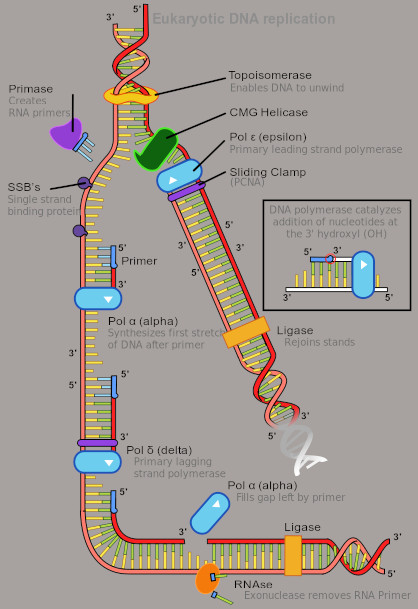
\includegraphics[width=0.7\linewidth]{./figures/replication/Eukaryotic_DNA_replication} 

}

\caption{\href{https://commons.wikimedia.org/wiki/File:Eukaryotic_DNA_replication.svg}{Many enzymes are involved in forming the DNA replication fork and DNA polymerization.}}\label{fig:repforkform}
\end{figure}

In G1 phase of the cell cycle, many of the DNA replication regulatory processes are initiated. In eukaryotes, the vast majority of DNA synthesis occurs during S phase of the cell cycle, and the entire genome must be unwound and duplicated to form two daughter copies. During G2, any damaged DNA or replication errors are corrected. Finally, one copy of the genomes is segregated to each daughter cell at mitosis or M phase. These daughter copies each contain one strand from the parental duplex DNA and one nascent antiparallel strand.

This mechanism is conserved from prokaryotes to eukaryotes and is known as semiconservative DNA replication. The process of semiconservative replication for the site of DNA replication is a fork-like DNA structure, the replication fork, where the DNA helix is open, or unwound, exposing unpaired DNA nucleotides for recognition and base pairing for the incorporation of free nucleotides into double-stranded DNA.

DNA replication, like all biological polymerization processes, proceeds in three enzymatically catalyzed and coordinated steps: initiation, elongation and termination.

\hypertarget{initiation}{%
\subsection{Initiation}\label{initiation}}

For a cell to divide, it must first replicate its DNA. DNA replication is an all-or-none process; once replication begins, it proceeds to completion. Once replication is complete, it does not occur again in the same cell cycle. This is made possible by the division of initiation into two temporally distinct steps: formation of the pre-replication complex and the preinitiation complex.

\hypertarget{pre-replication-complex}{%
\subsection{Pre-replication complex}\label{pre-replication-complex}}

In late mitosis and early G1 phase, a large complex of initiator proteins assembles into the pre-replication complex at particular points in the DNA, known as ``origins''. In E. coli the primary initiator protein is DnaA; in yeast, this is the origin recognition complex. Sequences used by initiator proteins tend to be ``AT-rich'' (rich in adenine and thymine bases), because A-T base pairs have two hydrogen bonds (rather than the three formed in a C-G pair) and thus are easier to strand-separate. In eukaryotes, the origin recognition complex catalyzes the assembly of initiator proteins into the pre-replication complex. Cdc6 and Cdt1 then associate with the bound origin recognition complex at the origin in order to form a larger complex necessary to load the Mcm complex onto the DNA. The Mcm complex is the helicase that will unravel the DNA helix at the replication origins and replication forks in eukaryotes. The Mcm complex is recruited at late G1 phase and loaded by the ORC-Cdc6-Cdt1 complex onto the DNA via ATP-dependent protein remodeling. The loading of the Mcm complex onto the origin DNA marks the completion of pre-replication complex formation.

If environmental conditions are right in late G1 phase, the G1 and G1/S cyclin-Cdk complexes are activated, which stimulate expression of genes that encode components of the DNA synthetic machinery. G1/S-Cdk activation also promotes the expression and activation of S-Cdk complexes, which may play a role in activating replication origins depending on species and cell type. Control of these Cdks vary depending cell type and stage of development. This regulation is best understood in budding yeast, where the S cyclins Clb5 and Clb6 are primarily responsible for DNA replication. Clb5,6-Cdk1 complexes directly trigger the activation of replication origins and are therefore required throughout S phase to directly activate each origin.

In a similar manner, Cdc7 is also required through S phase to activate replication origins. Cdc7 is not active throughout the cell cycle, and its activation is strictly timed to avoid premature initiation of DNA replication. In late G1, Cdc7 activity rises abruptly as a result of association with the regulatory subunit Dbf4, which binds Cdc7 directly and promotes its protein kinase activity. Cdc7 has been found to be a rate-limiting regulator of origin activity. Together, the G1/S-Cdks and/or S-Cdks and Cdc7 collaborate to directly activate the replication origins, leading to initiation of DNA synthesis.

\hypertarget{preinitiation-complex}{%
\subsection{Preinitiation complex}\label{preinitiation-complex}}

In early S phase, S-Cdk and Cdc7 activation lead to the assembly of the preinitiation complex, a massive protein complex formed at the origin. Formation of the preinitiation complex displaces Cdc6 and Cdt1 from the origin replication complex, inactivating and disassembling the pre-replication complex. Loading the preinitiation complex onto the origin activates the Mcm helicase, causing unwinding of the DNA helix. The preinitiation complex also loads α-primase and other DNA polymerases onto the DNA.

After α-primase synthesizes the first primers, the primer-template junctions interact with the clamp loader, which loads the sliding clamp onto the DNA to begin DNA synthesis. The components of the preinitiation complex remain associated with replication forks as they move out from the origin.

\hypertarget{elongation}{%
\subsection{Elongation}\label{elongation}}

DNA polymerase has 5′--3′ activity. All known DNA replication systems require a free 3′ hydroxyl group before synthesis can be initiated (note: the DNA template is read in 3′ to 5′ direction whereas a new strand is synthesized in the 5′ to 3′ direction---this is often confused). Four distinct mechanisms for DNA synthesis are recognized:

All cellular life forms and many DNA viruses, phages and plasmids use a primase to synthesize a short RNA primer with a free 3′ OH group which is subsequently elongated by a DNA polymerase.
The retroelements (including retroviruses) employ a transfer RNA that primes DNA replication by providing a free 3′ OH that is used for elongation by the reverse transcriptase.
In the adenoviruses and the φ29 family of bacteriophages, the 3′ OH group is provided by the side chain of an amino acid of the genome attached protein (the terminal protein) to which nucleotides are added by the DNA polymerase to form a new strand.
In the single stranded DNA viruses---a group that includes the circoviruses, the geminiviruses, the parvoviruses and others---and also the many phages and plasmids that use the rolling circle replication (RCR) mechanism, the RCR endonuclease creates a nick in the genome strand (single stranded viruses) or one of the DNA strands (plasmids). The 5′ end of the nicked strand is transferred to a tyrosine residue on the nuclease and the free 3′ OH group is then used by the DNA polymerase to synthesize the new strand.
The first is the best known of these mechanisms and is used by the cellular organisms. In this mechanism, once the two strands are separated, primase adds RNA primers to the template strands. The leading strand receives one RNA primer while the lagging strand receives several. The leading strand is continuously extended from the primer by a DNA polymerase with high processivity, while the lagging strand is extended discontinuously from each primer forming Okazaki fragments. RNase removes the primer RNA fragments, and a low processivity DNA polymerase distinct from the replicative polymerase enters to fill the gaps. When this is complete, a single nick on the leading strand and several nicks on the lagging strand can be found. Ligase works to fill these nicks in, thus completing the newly replicated DNA molecule.

The primase used in this process differs significantly between bacteria and archaea/eukaryotes. Bacteria use a primase belonging to the DnaG protein superfamily which contains a catalytic domain of the TOPRIM fold type. The TOPRIM fold contains an α/β core with four conserved strands in a Rossmann-like topology. This structure is also found in the catalytic domains of topoisomerase Ia, topoisomerase II, the OLD-family nucleases and DNA repair proteins related to the RecR protein.

The primase used by archaea and eukaryotes, in contrast, contains a highly derived version of the RNA recognition motif (RRM). This primase is structurally similar to many viral RNA-dependent RNA polymerases, reverse transcriptases, cyclic nucleotide generating cyclases and DNA polymerases of the A/B/Y families that are involved in DNA replication and repair. In eukaryotic replication, the primase forms a complex with Pol α.

Multiple DNA polymerases take on different roles in the DNA replication process. In E. coli, DNA Pol III is the polymerase enzyme primarily responsible for DNA replication. It assembles into a replication complex at the replication fork that exhibits extremely high processivity, remaining intact for the entire replication cycle. In contrast, DNA Pol I is the enzyme responsible for replacing RNA primers with DNA. DNA Pol I has a 5′ to 3′ exonuclease activity in addition to its polymerase activity, and uses its exonuclease activity to degrade the RNA primers ahead of it as it extends the DNA strand behind it, in a process called nick translation. Pol I is much less processive than Pol III because its primary function in DNA replication is to create many short DNA regions rather than a few very long regions.

In eukaryotes, the low-processivity enzyme, Pol α, helps to initiate replication because it forms a complex with primase. In eukaryotes, leading strand synthesis is thought to be conducted by Pol ε; however, this view has recently been challenged, suggesting a role for Pol δ. Primer removal is completed Pol δ while repair of DNA during replication is completed by Pol ε.

As DNA synthesis continues, the original DNA strands continue to unwind on each side of the bubble, forming a replication fork with two prongs. In bacteria, which have a single origin of replication on their circular chromosome, this process creates a ``theta structure'' (resembling the Greek letter theta: θ). In contrast, eukaryotes have longer linear chromosomes and initiate replication at multiple origins within these.

\hypertarget{replication-fork}{%
\subsection{Replication fork}\label{replication-fork}}

The replication fork is a structure that forms within the long helical DNA during DNA replication. It is created by helicases, which break the hydrogen bonds holding the two DNA strands together in the helix. The resulting structure has two branching ``prongs'', each one made up of a single strand of DNA. These two strands serve as the template for the leading and lagging strands, which will be created as DNA polymerase matches complementary nucleotides to the templates; the templates may be properly referred to as the leading strand template and the lagging strand template.

DNA is always synthesized in the 3′ to 5′ direction. Since the leading and lagging strad templates are oriented in opposite directions at the replication fork, a major issue is how to achieve synthesis of nascent (new) lagging strand DNA, whose direction of synthesis is opposite to the direction of the growing replication fork.

\hypertarget{leading-strand}{%
\subsection{Leading strand}\label{leading-strand}}

The leading strand is the strand of nascent DNA which is synthesized in the same direction as the growing replication fork. This sort of DNA replication is continuous.

\hypertarget{lagging-strand}{%
\subsection{Lagging strand}\label{lagging-strand}}

The lagging strand is the strand of nascent DNA whose direction of synthesis is opposite to the direction of the growing replication fork. Because of its orientation, replication of the lagging strand is more complicated as compared to that of the leading strand. As a consequence, the DNA polymerase on this strand is seen to ``lag behind'' the other strand.

The lagging strand is synthesized in short, separated segments. On the lagging strand template, a primase ``reads'' the template DNA and initiates synthesis of a short complementary RNA primer. A DNA polymerase extends the primed segments, forming Okazaki fragments. The RNA primers are then removed and replaced with DNA, and the fragments of DNA are joined together by DNA ligase.

In all cases the helicase is composed of six polypeptides that wrap around only one strand of the DNA being replicated. The two polymerases are bound to the helicase heximer. In eukaryotes the helicase wraps around the leading strand, and in prokaryotes it wraps around the lagging strand.

As helicase unwinds DNA at the replication fork, the DNA ahead is forced to rotate. This process results in a build-up of twists in the DNA ahead. This build-up forms a torsional resistance that would eventually halt the progress of the replication fork. Topoisomerases are enzymes that temporarily break the strands of DNA, relieving the tension caused by unwinding the two strands of the DNA helix; topoisomerases (including DNA gyrase) achieve this by adding negative supercoils to the DNA helix.

Bare single-stranded DNA tends to fold back on itself forming secondary structures; these structures can interfere with the movement of DNA polymerase. To prevent this, single-strand binding proteins bind to the DNA until a second strand is synthesized, preventing secondary structure formation.

Clamp proteins form a sliding clamp around DNA, helping the DNA polymerase maintain contact with its template, thereby assisting with processivity. The inner face of the clamp enables DNA to be threaded through it. Once the polymerase reaches the end of the template or detects double-stranded DNA, the sliding clamp undergoes a conformational change that releases the DNA polymerase. Clamp-loading proteins are used to initially load the clamp, recognizing the junction between template and RNA primers.:274-5

\hypertarget{dna-replication-proteins}{%
\section{DNA replication proteins}\label{dna-replication-proteins}}

At the replication fork, many replication enzymes assemble on the DNA into a complex molecular machine called the replisome. The following is a list of major DNA replication enzymes that participate in the replisome:

\begin{longtable}[t]{>{\raggedright\arraybackslash}p{10em}>{\raggedright\arraybackslash}p{30em}}
\caption{\label{tab:heteroploidy}A list of major DNA replication enzymes that participate in the replisome}\\
\toprule
Enzymes & Function in DNA replication\\
\midrule
\rowcolor{gray!6}  DNA helicase & Also known as helix destabilizing enzyme. Helicase separates the two strands of DNA at the Replication Fork behind the topoisomerase.\\
DNA polymerase & The enzyme responsible for catalyzing the addition of nucleotide substrates to DNA in the 5′ to 3′ direction during DNA replication. Also performs proof-reading and error correction. There exist many different types of DNA Polymerase, each of which perform different functions in different types of cells.\\
\rowcolor{gray!6}  DNA clamp & A protein which prevents elongating DNA polymerases from dissociating from the DNA parent strand.\\
Single-strand DNA-binding protein & Bind to ssDNA and prevent the DNA double helix from re-annealing after DNA helicase unwinds it, thus maintaining the strand separation, and facilitating the synthesis of the nascent strand.\\
\rowcolor{gray!6}  Topoisomerase & Relaxes the DNA from its super-coiled nature.\\
\addlinespace
DNA gyrase & Relieves strain of unwinding by DNA helicase; this is a specific type of topoisomerase\\
\rowcolor{gray!6}  DNA ligase & Re-anneals the semi-conservative strands and joins Okazaki Fragments of the lagging strand.\\
Primase & Provides a starting point of RNA (or DNA) for DNA polymerase to begin synthesis of the new DNA strand.\\
\rowcolor{gray!6}  Telomerase & Lengthens telomeric DNA by adding repetitive nucleotide sequences to the ends of eukaryotic chromosomes. This allows germ cells and stem cells to avoid the Hayflick limit on cell divisi\\
\bottomrule
\end{longtable}

Replication machineries consist of factors involved in DNA replication and appearing on template ssDNAs. Replication machineries include primosotors are replication enzymes; DNA polymerase, DNA helicases, DNA clamps and DNA topoisomerases, and replication proteins; e.g.~single-stranded DNA binding proteins (SSB). In the replication machineries these components coordinate. In most of the bacteria, all of the factors involved in DNA replication are located on replication forks and the complexes stay on the forks during DNA replication. These replication machineries are called replisomes or DNA replicase systems. These terms are generi terms for proteins located on replication forks. In eukaryotic and some bacterial cells the replisomes are not formed.

Since replication machineries do not move relatively to template DNAs such as factories, they are called a replication factory. In an alternative figure, DNA factories are similar to projectors and DNAs are like as cinematic films passing constantly into the projectors. In the replication factory model, after both DNA helicases for leading strands and lagging strands are loaded on the template DNAs, the helicases run along the DNAs into each other. The helicases remain associated for the remainder of replication process. Peter Meister et al.~observed directly replication sites in budding yeast by monitoring green fluorescent protein(GFP)-tagged DNA polymerases α. They detected DNA replication of pairs of the tagged loci spaced apart symmetrically from a replication origin and found that the distance between the pairs decreased markedly by time. This finding suggests that the mechanism of DNA replication goes with DNA factories. That is, couples of replication factories are loaded on replication origins and the factories associated with each other. Also, template DNAs move into the factories, which bring extrusion of the template ssDNAs and nascent DNAs. Meister's finding is the first direct evidence of replication factory model. Subsequent research has shown that DNA helicases form dimers in many eukaryotic cells and bacterial replication machineries stay in single intranuclear location during DNA synthesis.

The replication factories perform disentanglement of sister chromatids. The disentanglement is essential for distributing the chromatids into daughter cells after DNA replication. Because sister chromatids after DNA replication hold each other by Cohesin rings, there is the only chance for the disentanglement in DNA replication. Fixing of replication machineries as replication factories can improve the success rate of DNA replication. If replication forks move freely in chromosomes, catenation of nuclei is aggravated and impedes mitotic segregation.

\hypertarget{termination}{%
\subsection{Termination}\label{termination}}

Eukaryotes initiate DNA replication at multiple points in the chromosome, so replication forks meet and terminate at many points in the chromosome. Because eukaryotes have linear chromosomes, DNA replication is unable to reach the very end of the chromosomes. Due to this problem, DNA is lost in each replication cycle from the end of the chromosome. Telomeres are regions of repetitive DNA close to the ends and help prevent loss of genes due to this shortening. Shortening of the telomeres is a normal process in somatic cells. This shortens the telomeres of the daughter DNA chromosome. As a result, cells can only divide a certain number of times before the DNA loss prevents further division. (This is known as the Hayflick limit.) Within the germ cell line, which passes DNA to the next generation, telomerase extends the repetitive sequences of the telomere region to prevent degradation. Telomerase can become mistakenly active in somatic cells, sometimes leading to cancer formation. Increased telomerase activity is one of the hallmarks of cancer.

Termination requires that the progress of the DNA replication fork must stop or be blocked. Termination at a specific locus, when it occurs, involves the interaction between two components: (1) a termination site sequence in the DNA, and (2) a protein which binds to this sequence to physically stop DNA replication. In various bacterial species, this is named the DNA replication terminus site-binding protein, or Ter protein.

Because bacteria have circular chromosomes, termination of replication occurs when the two replication forks meet each other on the opposite end of the parental chromosome. E. coli regulates this process through the use of termination sequences that, when bound by the Tus protein, enable only one direction of replication fork to pass through. As a result, the replication forks are constrained to always meet within the termination region of the chromosome.

\hypertarget{regulation-of-replication}{%
\section{Regulation of replication}\label{regulation-of-replication}}

Within eukaryotes, DNA replication is controlled within the context of the cell cycle. As the cell grows and divides, it progresses through stages in the cell cycle; DNA replication takes place during the S phase (synthesis phase). The progress of the eukaryotic cell through the cycle is controlled by cell cycle checkpoints. Progression through checkpoints is controlled through complex interactions between various proteins, including cyclins and cyclin-dependent kinases. Unlike bacteria, eukaryotic DNA replicates in the confines of the nucleus.

The G1/S checkpoint (or restriction checkpoint) regulates whether eukaryotic cells enter the process of DNA replication and subsequent division. Cells that do not proceed through this checkpoint remain in the G0 stage and do not replicate their DNA.

After passing through the G1/S checkpoint, DNA must be replicated only once in each cell cycle. When the Mcm complex moves away from the origin, the pre-replication complex is dismantled. Because a new Mcm complex cannot be loaded at an origin until the pre-replication subunits are reactivated, one origin of replication can not be used twice in the same cell cycle.

Activation of S-Cdks in early S phase promotes the destruction or inhibition of individual pre-replication complex components, preventing immediate reassembly. S and M-Cdks continue to block pre-replication complex assembly even after S phase is complete, ensuring that assembly cannot occur again until all Cdk activity is reduced in late mitosis.

In budding yeast, inhibition of assembly is caused by Cdk-dependent phosphorylation of pre-replication complex components. At the onset of S phase, phosphorylation of Cdc6 by Cdk1 causes the binding of Cdc6 to the SCF ubiquitin protein ligase, which causes proteolytic destruction of Cdc6. Cdk-dependent phosphorylation of Mcm proteins promotes their export out of the nucleus along with Cdt1 during S phase, preventing the loading of new Mcm complexes at origins during a single cell cycle. Cdk phosphorylation of the origin replication complex also inhibits pre-replication complex assembly. The individual presence of any of these three mechanisms is sufficient to inhibit pre-replication complex assembly. However, mutations of all three proteins in the same cell does trigger reinitiation at many origins of replication within one cell cycle.

In animal cells, the protein geminin is a key inhibitor of pre-replication complex assembly. Geminin binds Cdt1, preventing its binding to the origin recognition complex. In G1, levels of geminin are kept low by the APC, which ubiquitinates geminin to target it for degradation. When geminin is destroyed, Cdt1 is released, allowing it to function in pre-replication complex assembly. At the end of G1, the APC is inactivated, allowing geminin to accumulate and bind Cdt1.

Replication of chloroplast and mitochondrial genomes occurs independently of the cell cycle, through the process of D-loop replication.

In vertebrate cells, replication sites concentrate into positions called replication foci. Replication sites can be detected by immunostaining daughter strands and replication enzymes and monitoring GFP-tagged replication factors. By these methods it is found that replication foci of varying size and positions appear in S phase of cell division and their number per nucleus is far smaller than the number of genomic replication forks.

P. Heun et al.,(2001) tracked GFP-tagged replication foci in budding yeast cells and revealed that replication origins move constantly in G1 and S phase and the dynamics decreased significantly in S phase. Traditionally, replication sites were fixed on spatial structure of chromosomes by nuclear matrix or lamins. The Heun's results denied the traditional concepts, budding yeasts don't have lamins, and support that replication origins self-assemble and form replication foci.

By firing of replication origins, controlled spatially and temporally, the formation of replication foci is regulated. D. A. Jackson et al.(1998) revealed that neighboring origins fire simultaneously in mammalian cells. Spatial juxtaposition of replication sites brings clustering of replication forks. The clustering do rescue of stalled replication forks and favors normal progress of replication forks. Progress of replication forks is inhibited by many factors; collision with proteins or with complexes binding strongly on DNA, deficiency of dNTPs, nicks on template DNAs and so on. If replication forks stall and the remaining sequences from the stalled forks are not replicated, the daughter strands have nick obtained un-replicated sites. The un-replicated sites on one parent's strand hold the other strand together but not daughter strands. Therefore, the resulting sister chromatids cannot separate from each other and cannot divide into 2 daughter cells. When neighboring origins fire and a fork from one origin is stalled, fork from other origin access on an opposite direction of the stalled fork and duplicate the un-replicated sites. As other mechanism of the rescue there is application of dormant replication origins that excess origins don't fire in normal DNA replication.

\hypertarget{prokaryotic-dna-replication}{%
\section{Prokaryotic DNA replication}\label{prokaryotic-dna-replication}}

Prokaryotic DNA replication is the process by which a prokaryote duplicates its DNA into another copy that is passed on to daughter cells. Although it is often studied in the model organism E. coli, other bacteria show many similarities. Replication is bi-directional and originates at a single origin of replication (OriC). It consists of three steps: Initiation, elongation, and termination.

\hypertarget{initiation-1}{%
\subsection{Initiation}\label{initiation-1}}

All cells must finish DNA replication before they can proceed for cell division. Media conditions that support fast growth in bacteria also couples with shorter inter-initiation time in them, i.e.~the doubling time in fast growing cells is less as compared to the slow growth. In other words, it is possible that in fast growth conditions the grandmother cells starts replicating its DNA for grand daughter cell. For the same reason, the initiation of DNA replication is highly regulated. Bacterial origins regulate orisome assembly, a nuclei-protein complex assembled on the origin responsible for unwinding the origin and loading all the replication machinery. In E. coli, the direction for orisome assembly are built into a short stretch of nucleotide sequence called as origin of replication (oriC) which contains multiple binding sites for the initiator protein DnaA (a highly homologous protein amongst bacterial kingdom). DnaA has four domains with each domain responsible for a specific task. There are 11 DnaA binding sites/boxes on the E. coli origin of replication out of which three boxes R1, R2 and R4 (which have a highly conserved 9 bp consensus sequence 5' - TTATC/ACACA ) are high affinity DnaA boxes. They bind to DnaA-ADP and DnaA-ATP with equal affinities and are bound by DnaA throughout most of the cell cycle and forms a scaffold on which rest of the orisome assembles. The rest eight DnaA boxes are low affinity sites that preferentially bind to DnaA-ATP. During initiation, DnaA bound to high affinity DnaA box R4 donates additional DnaA to the adjacent low affinity site and progressively fill all the low affinity DnaA boxes. Filling of the sites changes origin conformation from its native state. It is hypothesized that DNA stretching by DnaA bound to the origin promotes strand separation which allows more DnaA to bind to the unwound region. The DnaC helicase loader then interacts with the DnaA bound to the single-stranded DNA to recruit the DnaB helicase, which will continue to unwind the DNA as the DnaG primase lays down an RNA primer and DNA Polymerase III holoenzyme begins elongation.

Regulation
Chromosome replication in bacteria is regulated at the initiation stage. DnaA-ATP is hydrolyzed into the inactive DnaA-ADP by RIDA (Regulatory Inactivation of DnaA), and converted back to the active DnaA-ATP form by DARS (DnaA Reactivating Sequence, which is itself regulated by Fis and IHF). However, the main source of DnaA-ATP is synthesis of new molecules. Meanwhile, several other proteins interact directly with the oriC sequence to regulate initiation, usually by inhibition. In E. coli these proteins include DiaA, SeqA, IciA, HU, and ArcA-P, but they vary across other bacterial species. A few other mechanisms in E. coli that variously regulate initiation are DDAH (datA-Dependent DnaA Hydrolysis, which is also regulated by IHF), inhibition of the dnaA gene (by the SeqA protein), and reactivation of DnaA by the lipid membrane.

\hypertarget{elongation-1}{%
\subsection{Elongation}\label{elongation-1}}

Once priming is complete, DNA polymerase III holoenzyme is loaded into the DNA and replication begins. The catalytic mechanism of DNA polymerase III involves the use of two metal ions in the active site, and a region in the active site that can discriminate between deoxyribonucleotides and ribonucleotides. The metal ions are general divalent cations that help the 3' OH initiate a nucleophilic attack onto the alpha phosphate of the deoxyribonucleotide and orient and stabilize the negatively charged triphosphate on the deoxyribonucleotide. Nucleophilic attack by the 3' OH on the alpha phosphate releases pyrophosphate, which is then subsequently hydrolyzed (by inorganic phosphatase) into two phosphates. This hydrolysis drives DNA synthesis to completion.

Furthermore, DNA polymerase III must be able to distinguish between correctly paired bases and incorrectly paired bases. This is accomplished by distinguishing Watson-Crick base pairs through the use of an active site pocket that is complementary in shape to the structure of correctly paired nucleotides. This pocket has a tyrosine residue that is able to form van der Waals interactions with the correctly paired nucleotide. In addition, dsDNA (double stranded DNA) in the active site has a wider major groove and shallower minor groove that permits the formation of hydrogen bonds with the third nitrogen of purine bases and the second oxygen of pyrimidine bases. Finally, the active site makes extensive hydrogen bonds with the DNA backbone. These interactions result in the DNA polymerase III closing around a correctly paired base. If a base is inserted and incorrectly paired, these interactions could not occur due to disruptions in hydrogen bonding and van der Waals interactions.

DNA is read in the 3' → 5' direction, therefore, nucleotides are synthesized (or attached to the template strand) in the 5' → 3' direction. However, one of the parent strands of DNA is 3' → 5' while the other is 5' → 3'. To solve this, replication occurs in opposite directions. Heading towards the replication fork, the leading strand is synthesized in a continuous fashion, only requiring one primer. On the other hand, the lagging strand, heading away from the replication fork, is synthesized in a series of short fragments known as Okazaki fragments, consequently requiring many primers. The RNA primers of Okazaki fragments are subsequently degraded by RNase H and DNA Polymerase I (exonuclease), and the gaps (or nicks) are filled with deoxyribonucleotides and sealed by the enzyme ligase.

\hypertarget{rate-of-replication}{%
\subsection{Rate of replication}\label{rate-of-replication}}

The rate of DNA replication in a living cell was first measured as the rate of phage T4 DNA elongation in phage-infected E. coli. During the period of exponential DNA increase at 37 °C, the rate was 749 nucleotides per second. The mutation rate per base pair per replication during phage T4 DNA synthesis is 1.7 per 108.

\hypertarget{termination-1}{%
\subsection{Termination}\label{termination-1}}

Termination of DNA replication in E. coli is completed through the use of termination sequences and the Tus protein. These sequences allow the two replication forks to pass through in only one direction, but not the other.

DNA replication initially produces two catenated or linked circular DNA duplexes, each comprising one parental strand and one newly synthesised strand (by nature of semiconservative replication). This catenation can be visualised as two interlinked rings which cannot be separated. Topoisomerase 2 in E. coli unlinks or decatenates the two circular DNA duplexes by breaking the phosphodiester bonds present in two successive nucleotides of either parent DNA or newly formed DNA and thereafter the ligating activity ligates that broken DNA strand and so the two DNA get formed.



\chapter{Transcription And RNA Processing}\label{transcription-and-rna-processing}

\href{https://en.wikipedia.org/wiki/Transcription_(biology)}{Transcription} is the first of several steps of DNA based gene expression (gene is a short part of DNA that encodes for a protein), in which a particular segment of DNA is copied into RNA (especially mRNA) by the enzyme RNA polymerase. Both DNA and RNA are nucleic acids, which use base pairs of nucleotides as a complementary language. During transcription, a DNA sequence is read by an RNA polymerase, which produces a complementary, antiparallel RNA strand called a primary transcript.

Transcription proceeds in the following general steps:

\begin{enumerate}
\def\labelenumi{\arabic{enumi}.}
\tightlist
\item
  RNA polymerase, together with one or more general transcription factors, binds to promoter DNA.
\item
  RNA polymerase creates a transcription bubble, which separates the two strands of the DNA helix. This is done by breaking the hydrogen bonds between complementary DNA nucleotides.
\item
  RNA polymerase adds RNA nucleotides (which are complementary to the nucleotides of one DNA strand).
\item
  RNA sugar-phosphate backbone forms with assistance from RNA polymerase to form an RNA strand.
\item
  Hydrogen bonds of the RNA--DNA helix break, freeing the newly synthesized RNA strand.
\item
  If the cell has a nucleus, the RNA may be further processed. This may include polyadenylation, capping, and splicing.
\item
  The RNA may remain in the nucleus or exit to the cytoplasm through the nuclear pore complex.
\end{enumerate}

The stretch of DNA transcribed into an RNA molecule is called a transcription unit and encodes at least one gene. If the gene encodes a protein, the transcription produces messenger RNA (mRNA); the mRNA, in turn, serves as a template for the protein's synthesis through translation. Alternatively, the transcribed gene may encode for non-coding RNA such as microRNA, ribosomal RNA (rRNA), transfer RNA (tRNA), or enzymatic RNA molecules called ribozymes. Overall, RNA helps synthesize, regulate, and process proteins; it therefore plays a fundamental role in performing functions within a cell.

In virology, the term may also be used when referring to mRNA synthesis from an RNA molecule (i.e., RNA replication). For instance, the genome of a negative-sense single-stranded RNA (ssRNA -) virus may be template for a positive-sense single-stranded RNA (ssRNA +){[}clarification needed{]}. This is because the positive-sense strand contains the information needed to translate the viral proteins for viral replication afterwards. This process is catalyzed by a viral RNA replicase.{[}clarification needed{]}

A DNA transcription unit encoding for a protein may contain both a coding sequence, which will be translated into the protein, and regulatory sequences, which direct and regulate the synthesis of that protein. The regulatory sequence before (``upstream'' from) the coding sequence is called the five prime untranslated region (5'UTR); the sequence after (``downstream'' from) the coding sequence is called the three prime untranslated region (3'UTR).

As opposed to DNA replication, transcription results in an RNA complement that includes the nucleotide uracil (U) in all instances where thymine (T) would have occurred in a DNA complement.

Only one of the two DNA strands serve as a template for transcription. The antisense strand of DNA is read by RNA polymerase from the 3' end to the 5' end during transcription (3' → 5'). The complementary RNA is created in the opposite direction, in the 5' → 3' direction, matching the sequence of the sense strand with the exception of switching uracil for thymine. This directionality is because RNA polymerase can only add nucleotides to the 3' end of the growing mRNA chain. This use of only the 3' → 5' DNA strand eliminates the need for the Okazaki fragments that are seen in DNA replication. This also removes the need for an RNA primer to initiate RNA synthesis, as is the case in DNA replication.

The non-template (sense) strand of DNA is called the coding strand, because its sequence is the same as the newly created RNA transcript (except for the substitution of uracil for thymine). This is the strand that is used by convention when presenting a DNA sequence.

Transcription has some proofreading mechanisms, but they are fewer and less effective than the controls for copying DNA. As a result, transcription has a lower copying fidelity than DNA replication.

Transcription is divided into initiation, promoter escape, elongation, and termination.

\hypertarget{initiation-2}{%
\section{Initiation}\label{initiation-2}}

Transcription begins with the binding of RNA polymerase, together with one or more general transcription factors, to a specific DNA sequence referred to as a ``promoter'' to form an RNA polymerase-promoter ``closed complex''. In the ``closed complex'' the promoter DNA is still fully double-stranded.

RNA polymerase, assisted by one or more general transcription factors, then unwinds approximately 14 base pairs of DNA to form an RNA polymerase-promoter ``open complex''. In the ``open complex'' the promoter DNA is partly unwound and single-stranded. The exposed, single-stranded DNA is referred to as the ``transcription bubble.''

RNA polymerase, assisted by one or more general transcription factors, then selects a transcription start site in the transcription bubble, binds to an initiating NTP and an extending NTP (or a short RNA primer and an extending NTP) complementary to the transcription start site sequence, and catalyzes bond formation to yield an initial RNA product.

In bacteria, RNA polymerase holoenzyme consists of five subunits: 2 α subunits, 1 β subunit, 1 β' subunit, and 1 ω subunit. In bacteria, there is one general RNA transcription factor known as a sigma factor. RNA polymerase core enzyme binds to the bacterial general transcription (sigma) factor to form RNA polymerase holoenzyme and then binds to a promoter. (RNA polymerase is called a holoenzyme when sigma subunit is attached to the core enzyme which is consist of 2 α subunits, 1 β subunit, 1 β' subunit only).

In archaea and eukaryotes, RNA polymerase contains subunits homologous to each of the five RNA polymerase subunits in bacteria and also contains additional subunits. In archaea and eukaryotes, the functions of the bacterial general transcription factor sigma are performed by multiple general transcription factors that work together. In archaea, there are three general transcription factors: TBP, TFB, and TFE. In eukaryotes, in RNA polymerase II-dependent transcription, there are six general transcription factors: TFIIA, TFIIB (an ortholog of archaeal TFB), TFIID (a multisubunit factor in which the key subunit, TBP, is an ortholog of archaeal TBP), TFIIE (an ortholog of archaeal TFE), TFIIF, and TFIIH. The TFIID is the first component to bind to DNA due to binding of TBP, while TFIIH is the last component to be recruited. In archaea and eukaryotes, the RNA polymerase-promoter closed complex is usually referred to as the ``preinitiation complex.''

Transcription initiation is regulated by additional proteins, known as activators and repressors, and, in some cases, associated coactivators or corepressors, which modulate formation and function of the transcription initiation complex.

After the first bond is synthesized, the RNA polymerase must escape the promoter. During this time there is a tendency to release the RNA transcript and produce truncated transcripts. This is called abortive initiation, and is common for both eukaryotes and prokaryotes. Abortive initiation continues to occur until an RNA product of a threshold length of approximately 10 nucleotides is synthesized, at which point promoter escape occurs and a transcription elongation complex is formed.

Mechanistically, promoter escape occurs through DNA scrunching, providing the energy needed to break interactions between RNA polymerase holoenzyme and the promoter.

In bacteria, it was historically thought that the sigma factor is definitely released after promoter clearance occurs. This theory had been known as the obligate release model however later data showed that upon and following promoter clearance, the sigma factor is released according to a stochastic model known as the stochastic release model.

In eukaryotes, at an RNA polymerase II-dependent promoter, upon promoter clearance, TFIIH phosphorylates serine 5 on the carboxy terminal domain of RNA polymerase II, leading to the recruitment of capping enzyme (CE). The exact mechanism of how CE induces promoter clearance in eukaryotes is not yet known.

\hypertarget{elongation-2}{%
\section{Elongation}\label{elongation-2}}

One strand of the DNA, the template strand (or noncoding strand), is used as a template for RNA synthesis. As transcription proceeds, RNA polymerase traverses the template strand and uses base pairing complementarity with the DNA template to create an RNA copy (which elongates during the traversal). Although RNA polymerase traverses the template strand from 3' → 5', the coding (non-template) strand and newly formed RNA can also be used as reference points, so transcription can be described as occurring 5' → 3'. This produces an RNA molecule from 5' → 3', an exact copy of the coding strand (except that thymines are replaced with uracils, and the nucleotides are composed of a ribose (5-carbon) sugar where DNA has deoxyribose (one fewer oxygen atom) in its sugar-phosphate backbone).{[}citation needed{]}



\begin{figure}

{\centering 
\includegraphics[width=0.7\linewidth]{./figures/transcription/Simple_transcription_elongation1} 

}

\caption{\href{https://commons.wikimedia.org/wiki/File:Simple_transcription_elongation1.svg}{RNA polymerase (RNAP) at work. Note the coding and template strands. The resulting RNA is a synthesized from the template strand and identical in sequence to the coding strand.}}\label{fig:elongation}
\end{figure}

mRNA transcription can involve multiple RNA polymerases on a single DNA template and multiple rounds of transcription (amplification of particular mRNA), so many mRNA molecules can be rapidly produced from a single copy of a gene.{[}citation needed{]} The characteristic elongation rates in prokaryotes and eukaryotes are about 10-100 nts/sec.~In eukaryotes, however, nucleosomes act as major barriers to transcribing polymerases during transcription elongation. In these organisms, the pausing induced by nucleosomes can be regulated by transcription elongation factors such as TFIIS.

Elongation also involves a proofreading mechanism that can replace incorrectly incorporated bases. In eukaryotes, this may correspond with short pauses during transcription that allow appropriate RNA editing factors to bind. These pauses may be intrinsic to the RNA polymerase or due to chromatin structure.{[}citation needed{]}

\hypertarget{termination-2}{%
\section{Termination}\label{termination-2}}

Bacteria use two different strategies for transcription termination -- Rho-independent termination and Rho-dependent termination. In Rho-independent transcription termination, RNA transcription stops when the newly synthesized RNA molecule forms a G-C-rich hairpin loop followed by a run of Us. When the hairpin forms, the mechanical stress breaks the weak rU-dA bonds, now filling the DNA--RNA hybrid. This pulls the poly-U transcript out of the active site of the RNA polymerase, terminating transcription. In the ``Rho-dependent'' type of termination, a protein factor called ``Rho'' destabilizes the interaction between the template and the mRNA, thus releasing the newl synthesized mRNA from the elongation complex.

Transcription termination in eukaryotes is less well understood than in bacteria, but involves cleavage of the new transcript followed by template-independent addition of adenines at its new 3' end, in a process called polyadenylation.

\hypertarget{inhibitors-of-transcription}{%
\section{Inhibitors of transcription}\label{inhibitors-of-transcription}}

Transcription inhibitors can be used as antibiotics against, for example, pathogenic bacteria (antibacterials) and fungi (antifungals). An example of such an antibacterial is rifampicin, which inhibits bacterial transcription of DNA into mRNA by inhibiting DNA-dependent RNA polymerase by binding its beta-subunit, while 8-hydroxyquinoline is an antifungal transcription inhibitor. The effects of histone methylation may also work to inhibit the action of transcription.

In vertebrates, the majority of gene promoters contain a CpG island with numerous CpG sites. When many of a gene's promoter CpG sites are methylated the gene becomes inhibited (silenced). Colorectal cancers typically have 3 to 6 driver mutations and 33 to 66 hitchhiker or passenger mutations. However, transcriptional inhibition (silencing) may be of more importance than mutation in causing progression to cancer. For example, in colorectal cancers about 600 to 800 genes are transcriptionally inhibited by CpG island methylation (see regulation of transcription in cancer). Transcriptional repression in cancer can also occur by other epigenetic mechanisms, such as altered expression of microRNAs. In breast cancer, transcriptional repression of BRCA1 may occur more frequently by over-expressed microRNA-182 than by hypermethylation of the BRCA1 promoter (see Low expression of BRCA1 in breast and ovarian cancers).

\hypertarget{transcription-factors}{%
\section{Transcription factors}\label{transcription-factors}}

Active transcription units are clustered in the nucleus, in discrete sites called transcription factories or euchromatin. Such sites can be visualized by allowing engaged polymerases to extend their transcripts in tagged precursors (Br-UTP or Br-U) and immuno-labeling the tagged nascent RNA. Transcription factories can also be localized using fluorescence in situ hybridization or marked by antibodies directed against polymerases. There are \textasciitilde{}10,000 factories in the nucleoplasm of a HeLa cell, among which are \textasciitilde{}8,000 polymerase II factories and \textasciitilde{}2,000 polymerase III factories. Each polymerase II factory contains \textasciitilde{}8 polymerases. As most active transcription units are associated with only one polymerase, each factory usually contains \textasciitilde{}8 different transcription units. These units might be associated through promoters and/or enhancers, with loops forming a ``cloud'' around the factor.

A molecule that allows the genetic material to be realized as a protein was first hypothesized by François Jacob and Jacques Monod. Severo Ochoa won a Nobel Prize in Physiology or Medicine in 1959 for developing a process for synthesizing RNA in vitro with polynucleotide phosphorylase, which was useful for cracking the genetic code. RNA synthesis by RNA polymerase was established in vitro by several laboratories by 1965; however, the RNA synthesized by these enzymes had properties that suggested the existence of an additional factor needed to terminate transcription correctly.{[}citation needed{]}

In 1972, Walter Fiers became the first person to actually prove the existence of the terminating enzyme.

Roger D. Kornberg won the 2006 Nobel Prize in Chemistry ``for his studies of the molecular basis of eukaryotic transcription''.

\hypertarget{rna-processing}{%
\section{RNA Processing}\label{rna-processing}}

\href{https://en.wikipedia.org/wiki/Post-transcriptional_modification}{Post-transcriptional modification} or co-transcriptional modification is a set of biological processes common to most eukaryotic cells by which an RNA primary transcript is chemically altered following transcription from a gene to produce a mature, functional RNA molecule that can then leave the nucleus and perform any of a variety of different functions in the cell. {[}1{]} There are many types of post-transcriptional modifications achieved through a diverse class of molecular mechanisms.

Perhaps the most notable example is the conversion of precursor messenger RNA transcripts into mature messenger RNA that is subsequently capable of being translated into protein. This process includes three major steps that significantly modify the chemical structure of the RNA molecule: the addition of a 5' cap, the addition of a 3' polyadenylated tail, and RNA splicing. Such processing is vital for the correct translation of eukaryotic genomes because the initial precursor mRNA produced by transcription often contains both exons (coding sequences) and introns (non-coding sequences); splicing removes the introns and links the exons directly, while the cap and tail facilitate the transport of the mRNA to a ribosome and protect it from molecular degradation.{[}2{]}

Post-transcriptional modifications may also occur during the processing of other transcripts which ultimately become transfer RNA, ribosomal RNA, or any of the other types of RNA used by the cell.

\hypertarget{mrna-processing}{%
\section{mRNA processing}\label{mrna-processing}}

The pre-mRNA molecule undergoes three main modifications. These modifications are 5' capping, 3' polyadenylation, and RNA splicing, which occur in the cell nucleus before the RNA is translated.{[}4{]}

\hypertarget{processing}{%
\subsection{5' processing}\label{processing}}

Capping of the pre-mRNA involves the addition of 7-methylguanosine (m7G) to the 5' end. To achieve this, the terminal 5' phosphate requires removal, which is done with the aid of a phosphatase enzyme. The enzyme guanosyl transferase then catalyses the reaction, which produces the diphosphate 5' end. The diphosphate 5' end then attacks the alpha phosphorus atom of a GTP molecule in order to add the guanine residue in a 5'5' triphosphate link. The enzyme (guanine-N7-)-methyltransferase (``cap MTase'') transfers a methyl group from S-adenosyl methionine to the guanine ring.{[}5{]} This type of cap, with just the (m7G) in position is called a cap 0 structure. The ribose of the adjacent nucleotide may also be methylated to give a cap 1. Methylation of nucleotides downstream of the RNA molecule produce cap 2, cap 3 structures and so on. In these cases the methyl groups are added to the 2' OH groups of the ribose sugar. The cap protects the 5' end of the primary RNA transcript from attack by ribonucleases that have specificity to the 3'5' phosphodiester bonds.{[}6{]}

\hypertarget{processing-1}{%
\subsection{3' processing}\label{processing-1}}

The pre-mRNA processing at the 3' end of the RNA molecule involves cleavage of its 3' end and then the addition of about 250 adenine residues to form a poly(A) tail. The cleavage and adenylation reactions occur primarily if a polyadenylation signal sequence (5'- AAUAAA-3') is located near the 3' end of the pre-mRNA molecule, which is followed by another sequence, which is usually (5'-CA-3') and is the site of cleavage. A GU-rich sequence is also usually present further downstream on the pre-mRNA molecule. More recently, it has been demonstrated that alternate signal sequences such as UGUA upstream off the cleavage site can also direct cleavage and polyadenylation in the absence of the AAUAAA signal. It is important to understand that these two signals are not mutually independent and often coexist. After the synthesis of the sequence elements, several multi-subunit proteins are transferred to the RNA molecule. The transfer of these sequence specific binding proteins cleavage and polyadenylation specificity factor (CPSF), Cleavage Factor I (CF I) and cleavage stimulation factor (CStF) occurs from RNA Polymerase II. The three factors bind to the sequence elements. The AAUAAA signal is directly bound by CPSF. For UGUA dependent processing sites, binding of the multi protein complex is done by Cleavage Factor I (CF I). The resultant protein complex formed contains additional cleavage factors and the enzyme Polyadenylate Polymerase (PAP). This complex cleaves the RNA between the polyadenylation sequence and the GU-rich sequence at the cleavage site marked by the (5'-CA-3') sequences. Poly(A) polymerase then adds about 200 adenine units to the new 3' end of the RNA molecule using ATP as a precursor. As the poly(A) tail is synthesised, it binds multiple copies of poly(A) binding protein, which protects the 3'end from ribonuclease digestion.{[}6{]}

\hypertarget{introns-splicing}{%
\subsection{Introns Splicing}\label{introns-splicing}}

RNA splicing is the process by which introns, regions of RNA that do not code for proteins, are removed from the pre-mRNA and the remaining exons connected to re-form a single continuous molecule. Exons are sections of mRNA which become ``expressed'' or translated into a protein. They are the coding portions of a mRNA molecule.{[}7{]} Although most RNA splicing occurs after the complete synthesis and end-capping of the pre-mRNA, transcripts with many exons can be spliced co-transcriptionally.{[}8{]} The splicing reaction is catalyzed by a large protein complex called the spliceosome assembled from proteins and small nuclear RNA molecules that recognize splice sites in the pre-mRNA sequence. Many pre-mRNAs, including those encoding antibodies, can be spliced in multiple ways to produce different mature mRNAs that encode different protein sequences. This process is known as alternative splicing, and allows production of a large variety of proteins from a limited amount of DNA.

\hypertarget{reverse-transcription}{%
\section{Reverse transcription}\label{reverse-transcription}}

Some viruses (such as HIV, the cause of AIDS), have the ability to transcribe RNA into DNA. HIV has an RNA genome that is reverse transcribed into DNA. The resulting DNA can be merged with the DNA genome of the host cell. The main enzyme responsible for synthesis of DNA from an RNA template is called reverse transcriptase.

In the case of HIV, reverse transcriptase is responsible for synthesizing a complementary DNA strand (cDNA) to the viral RNA genome. The enzyme ribonuclease H then digests the RNA strand, and reverse transcriptase synthesises a complementary strand of DNA to form a double helix DNA structure (``cDNA''). The cDNA is integrated into the host cell's genome by the enzyme integrase, which causes the host cell to generate viral proteins that reassemble into new viral particles. In HIV, subsequent to this, the host cell undergoes programmed cell death, or apoptosis of T cells. However, in other retroviruses, the host cell remains intact as the virus buds out of the cell.

Some eukaryotic cells contain an enzyme with reverse transcription activity called telomerase. Telomerase is a reverse transcriptase that lengthens the ends of linear chromosomes. Telomerase carries an RNA template from which it synthesizes a repeating sequence of DNA, or ``junk'' DNA. This repeated sequence of DNA is called a telomere and can be thought of as a ``cap'' for a chromosome. It is important because every time a linear chromosome is duplicated, it is shortened. With this ``junk'' DNA or ``cap'' at the ends of chromosomes, the shortening eliminates some of the non-essential, repeated sequence rather than the protein-encoding DNA sequence, that is farther away from the chromosome end.

Telomerase is often activated in cancer cells to enable cancer cells to duplicate their genomes indefinitely without losing important protein-coding DNA sequence. Activation of telomerase could be part of the process that allows cancer cells to become immortal. The immortalizing factor of cancer via telomere lengthening due to telomerase has been proven to occur in 90\% of all carcinogenic tumors in vivo with the remaining 10\% using an alternative telomere maintenance route called ALT or Alternative Lengthening of Telomeres.



\chapter{Translation And The Genetic Code}\label{translation-and-the-genetic-code}

In molecular biology and genetics, \href{https://en.wikipedia.org/wiki/Translation_(biology)}{translation} is the process in which ribosomes in the cytoplasm or ER synthesize proteins after the process of transcription of DNA to RNA in the cell's nucleus. The entire process is called gene expression.

In translation, messenger RNA (mRNA) is decoded in the ribosome decoding center to produce a specific amino acid chain, or polypeptide. The polypeptide later folds into an active protein and performs its functions in the cell. The ribosome facilitates decoding by inducing the binding of complementary tRNA anticodon sequences to mRNA codons. The tRNAs carry specific amino acids that are chained together into a polypeptide a the mRNA passes through and is read by the ribosome.

Translation proceeds in three phases:

\begin{enumerate}
\def\labelenumi{\arabic{enumi}.}
\tightlist
\item
  \textbf{Initiation:} The ribosome assembles around the target mRNA. The first tRNA is attached at the start codon.
\item
  \textbf{Elongation:} The tRNA transfers an amino acid to the tRNA corresponding to the next codon. The ribosome then moves (translocates) to the next mRNA codon to continue the process, creating an amino acid chain.
\item
  \textbf{Termination:} When a peptidyl tRNA encounters a stop codon, then the ribosome folds the polypeptide into its final structure.
\end{enumerate}



\begin{figure}

{\centering 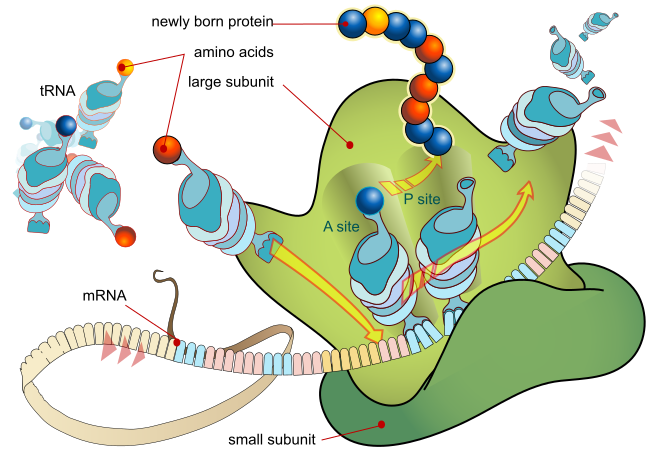
\includegraphics[width=0.7\linewidth]{./figures/translation/Ribosome_mRNA_translation_en} 

}

\caption{\href{https://commons.wikimedia.org/wiki/File:Ribosome_mRNA_translation_en.svg}{Diagram showing the translation of mRNA and the synthesis of proteins by a ribosome.}}\label{fig:translation}
\end{figure}

In prokaryotes, translation occurs in the cytosol, where the medium and small subunits of the ribosome bind to the tRNA. In eukaryotes, translation occurs in the cytosol or across the membrane of the endoplasmic reticulum in a process called co-translational translocation. In co-translational translocation, the entire ribosome/mRNA complex binds to the outer membrane of the rough endoplasmic reticulum (ER) and the new protein is synthesized and released into the ER; the newly created polypeptide can be stored inside the ER for future vesicle transport and secretion outside the cell, or immediately secreted.

Many types of transcribed RNA, such as transfer RNA, ribosomal RNA, and small nuclear RNA, do not undergo translation into proteins.

A number of antibiotics act by inhibiting translation. These include clindamycin, anisomycin, cycloheximide, chloramphenicol, tetracycline, streptomycin, erythromycin, and puromycin. Prokaryotic ribosomes have a different structure from that of eukaryotic ribosomes, and thus antibiotics can specifically target bacterial infections without any harm to a eukaryotic host's cells.

In 1954, Zamecnik and Hoagland discovered tRNA. In 1955, George E. Palade discovered ribosomes.

The basic process of translation is the addition of one amino acid at a time to the end of the polypeptide being formed. This process takes place inside the ribosome.

\hypertarget{eukaryotic-translation}{%
\section{Eukaryotic translation}\label{eukaryotic-translation}}

\hypertarget{initiation-3}{%
\subsection{Initiation}\label{initiation-3}}

Initiation of translation usually involves the interaction of certain key proteins, the initiation factors, with a special tag bound to the 5'-end of an mRNA molecule, the 5' cap, as well as with the 5' UTR. These proteins bind the small (40S) ribosomal subunit and hold the mRNA in place. eIF3 is associated with the 40S ribosomal subunit and plays a role in keeping the large (60S) ribosomal subunit from prematurely binding. eIF3 also interacts with the eIF4F complex, which consists of three other initiation factors: eIF4A, eIF4E, and eIF4G. eIF4G is a scaffolding protein that directly associates with both eIF3 and the other two components. eIF4E is the cap-binding protein. Binding of the cap by eIF4E is often considered the rate-limiting step of cap-dependent initiation, and the concentration of eIF4E is a regulatory nexus of translational control. Certain viruses cleave a portion of eIF4G that binds eIF4E, thus preventing cap-dependent translation to hijack the host machinery in favor of the viral (cap-independent) messages. eIF4A is an ATP-dependent RNA helicase that aids the ribosome by resolving certain secondary structures formed along the mRNA transcript. The poly(A)-binding protein (PABP) also associates with the eIF4F complex via eIF4G, and binds the poly-A tail of most eukaryotic mRNA molecules. This protein has been implicated in playing a role in circularization of the mRNA during translation. This 43S preinitiation complex (43S PIC) accompanied by the protein factors moves along the mRNA chain toward its 3'-end, in a process known as `scanning', to reach the start codon (typically AUG). In eukaryotes and archaea, the amino acid encoded by the start codon is methionine. The Met-charged initiator tRNA (Met-tRNAiMet) is brought to the P-site of the small ribosomal subunit by eukaryotic initiation factor 2 (eIF2). It hydrolyzes GTP, and signals for the dissociation of several factors from the small ribosomal subunit, eventually leading to the association of the large subunit (or the 60S subunit). The complete ribosome (80S) then commences translation elongation. Regulation of protein synthesis is partly influenced by phosphorylation of eIF2 (via the α subunit), which is a part of the eIF2-GTP-Met-tRNAiMet ternary complex (eIF2-TC). When large numbers of eIF2 are phosphorylated, protein synthesis is inhibited. This occurs under amino acid starvation or after viral infection. However, a small fraction of this initiation factor is naturally phosphorylated. Another regulator is 4EBP, which binds to the initiation factor eIF4E and inhibits its interactions with eIF4G, thus preventing cap-dependent initiation. To oppose the effects of 4EBP, growth factors phosphorylate 4EBP, reducing its affinity for eIF4E and permitting protein synthesis. While protein synthesis is globally regulated by modulating the expression of key initiation factors as well as the number of ribosomes, individual mRNAs can have different translation rates due to the presence of regulatory sequence elements. This has been shown to be important in a variety of settings including yeast meiosis and ethylene response in plants. In addition, recent work in yeast and humans suggest that evolutionary divergence in cis-regulatory sequences can impact translation regulation. Additionally, RNA helicases such as DHX29 and Ded1/DDX3 may participate in the process of translation initiation, especially for mRNAs with structured 5'UTRs.

Cap-independent initiation
The best-studied example of cap-independent translation initiation in eukaryotes is that by the Internal ribosome entry site (IRES). What differentiates cap-independent translation from cap-dependent translation is that cap-independent translation does not require the 5' cap to initiate scanning from the 5' end of the mRNA until the start codon. The ribosome can be trafficked to the start site by direct binding, initiation factors, and/or ITAFs (IRES trans-acting factors) bypassing the need to scan the entire 5' UTR. This method of translation has been found important in conditions that require the translation of specific mRNAs during cellular stress, when overall translation is reduced. Examples include factors responding to apoptosis and stress-induced responses.

\hypertarget{elongation-3}{%
\subsection{Elongation}\label{elongation-3}}

Elongation depends on eukaryotic elongation factors. At the end of the initiation step, the mRNA is positioned so that the next codon can be translated during the elongation stage of protein synthesis. The initiator tRNA occupies the P site in the ribosome, and the A site is ready to receive an aminoacyl-tRNA. During chain elongation, each additional amino acid is added to the nascent polypeptide chain in a three-step microcycle. The steps in this microcycle are (1) positioning the correct aminoacyl-tRNA in the A site of the ribosome, (2) forming the peptide bond and (3) shifting the mRNA by one codon relative to the ribosome. Unlike bacteria, in which translation initiation occurs as soon as the 5' end of an mRNA is synthesized, in eukaryotes such tight coupling between transcription and translation is not possible because transcription and translation are carried out in separate compartments of the cell (the nucleus and cytoplasm). Eukaryotic mRNA precursors must be processed in the nucleus (e.g., capping, polyadenylation, splicing) before they are exported to the cytoplasm for translation. Translation can also be affected by ribosomal pausing, which can trigger endonucleolytic attack of the mRNA, a process termed mRNA no-go decay. Ribosomal pausing also aids co-translational folding of the nascent polypeptide on the ribosome, and delays protein translation while it is encoding mRNA. This can trigger ribosomal frameshifting.

\hypertarget{termination-3}{%
\subsection{Termination}\label{termination-3}}

Termination of elongation depends on eukaryotic release factors. The process is similar to that of prokaryotic termination, but unlike prokaryotic termination, there is a universal release factor, eRF1, that recognizes all three stop codons. Upon termination, the ribosome is disassembled and the completed polypeptide is released. eRF3 is a ribosome-dependent GTPase that helps eRF1 release the completed polypeptide. The human genome encodes a few genes whose mRNA stop codon are surprisingly leaky: In these genes, termination of translation is inefficient due to special RNA bases in the vicinity of the stop codon. Leaky termination in these genes leads to translational readthrough of up to 10\% of the stop codons of these genes. Some of these genes encode functional protein domains in their readthrough extension so that new protein isoforms can arise. This process has been termed `functional translational readthrough'.

\hypertarget{ribosomes}{%
\section{Ribosomes}\label{ribosomes}}

\href{https://en.wikipedia.org/wiki/Ribosome}{Ribosomes} are complex macromolecular machines, found within all living cells, that serves as the site of biological protein synthesis. Ribosomes link amino acids together in the order specified by messenger RNA (RNA) molecules. Ribosomes consist of two major components: the small ribosomal subunits, which read the mRNA, and the large subunits, which join amino acids to form a polypeptide chain. Each subunit consists of one or more ribosomal RNA (rRNA) molecules and a variety of ribosomal proteins. The ribosomes and associated molecules are also known as the translational apparatus.

The sequence of DNA, which encodes the sequence of the amino acids in a protein, is copied into a messenger RNA chain. It may be copied many times into RNA chains. Ribosomes can bind to a messenger RNA chain and use its sequence for determining the correct sequence of amino acids for generating a given protein. Amino acids are selected and collected and carried to the ribosome by transfer RNA (tRNA) molecules, which enter one part of the ribosome and bind to the messenger RNA chain. It is during this binding that the correct translation of nucleic acid sequence to amino acid sequence occurs. For each coding triplet in the messenger RNA there is a distinct transfer RNA that matches and which carries the correct amino acid for that coding triplet. The attached amino acids are then linked together by another part of the ribosome. Once the protein is produced, it can then fold to produce a specific functional three-dimensional structure although during synthesis some proteins start folding into their correct form.

A ribosome is made from complexes of RNAs and proteins and is therefore a ribonucleoprotein. Each ribosome is divided into two subunits:

\begin{enumerate}
\def\labelenumi{\arabic{enumi}.}
\tightlist
\item
  a smaller subunit which binds to a larger subunit and the mRNA pattern, and
\item
  a larger subunit which binds to the tRNA, the amino acids, and the smaller subunit.
\end{enumerate}

When a ribosome finishes reading an mRNA molecule, these two subunits split apart. Ribosomes are ribozymes, because the catalytic peptidyl transferase activity that links amino acids together is performed by the ribosomal RNA. Ribosomes are often associated with the intracellular membranes that make up the rough endoplasmic reticulum.

Ribosomes from bacteria, archaea and eukaryotes in the three-domain system, resemble each other to a remarkable degree, evidence of a common origin. They differ in their size, sequence, structure, and the ratio of protein to RNA. The differences in structure allow some antibiotics to kill bacteria by inhibiting their ribosomes, while leaving human ribosomes unaffected. In bacteria and archaea, more than one ribosome may move along a single mRNA chain at one time, each ``reading'' its sequence and producing a corresponding protein molecule.

The mitochondrial ribosomes of eukaryotic cells, are produced from mitochondrial genes, and functionally resemble many features of those in bacteria, reflecting the likely evolutionary origin of mitochondria.

Ribosomes were first observed in the mid-1950s by Romanian-American cell biologist George Emil Palade, using an electron microscope, as dense particles or granules. The term ``ribosome'' was proposed by scientist Richard B. Roberts in the end of 1950s.

Albert Claude, Christian de Duve, and George Emil Palade were jointly awarded the Nobel Prize in Physiology or Medicine, in 1974, for the discovery of the ribosome. The Nobel Prize in Chemistry 2009 was awarded to Venkatraman Ramakrishnan, Thomas A. Steitz and Ada E. Yonath for determining the detailed structure and mechanism of the ribosome.

The ribosome is a highly complex cellular machine. It is largely made up of specialized RNA known as ribosomal RNA (rRNA) as well as dozens of distinct proteins (the exact number varies slightly between species). The ribosomal proteins and rRNAs are arranged into two distinct ribosomal pieces of different size, known generally as the large and small subunit of the ribosome. Ribosomes consist of two subunits that fit together (Figure 2) and work as one to translate the mRNA into a polypeptide chain during protein synthesis (Figure 1). Because they are formed from two subunits of non-equal size, they are slightly longer in the axis than in diameter.

\hypertarget{bacterial-ribosomes}{%
\section{Bacterial ribosomes}\label{bacterial-ribosomes}}

Prokaryotic ribosomes are around 20 nm (200 Å) in diameter and are composed of 65\% rRNA and 35\% ribosomal proteins. Eukaryotic ribosomes are between 25 and 30 nm (250--300 Å) in diameter with an rRNA-to-protein ratio that is close to 1. Crystallographic work has shown that there are no ribosomal proteins close to the reaction site for polypeptide synthesis. This suggests that the protein components of ribosomes do not directly participate in peptide bond formation catalysis, but rather that these proteins act as a scaffold that may enhance the ability of rRNA to synthesize protein



\begin{figure}

{\centering 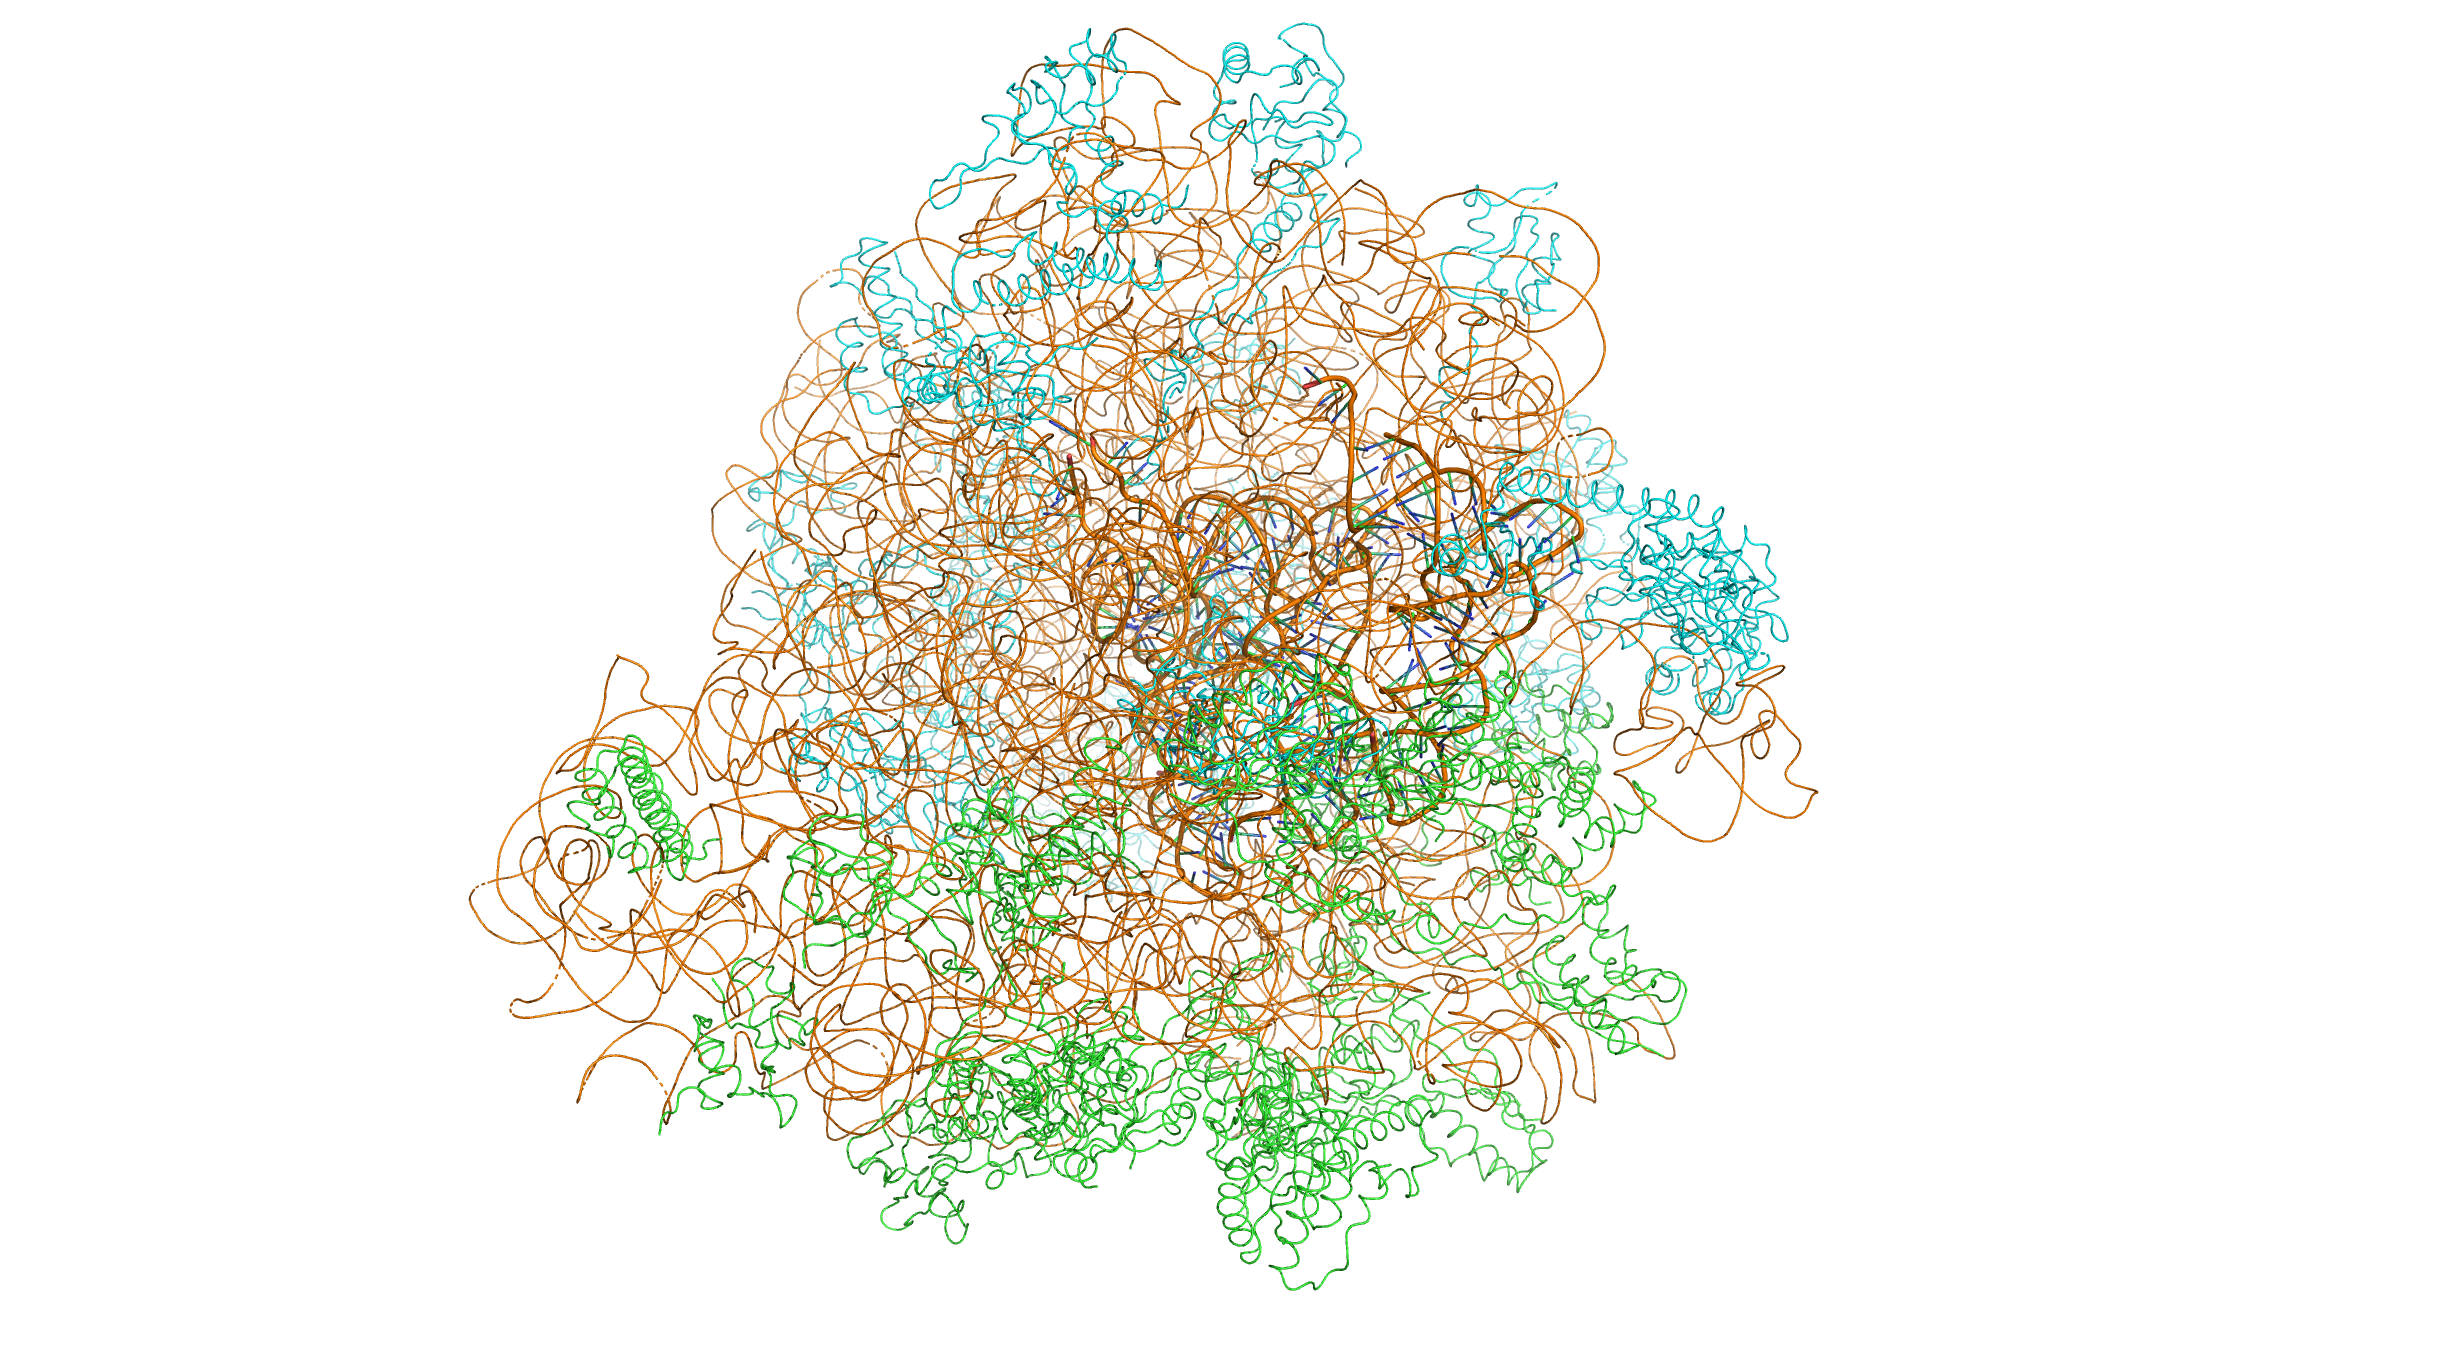
\includegraphics[width=0.7\linewidth]{./figures/translation/ttribosome} 

}

\caption{Crystal structure of the bacterial 70S ribosome of the bacterium \emph{Thermus thermophilus}. The 30S (small) ribosomal subunit proteins are colored in green, the 50S (large) subunit proteins are colored in blue, the ribosomal RNA is colored orange. The 30S subunits contains 3 tRNA molecules (based on atomic coordinates of \href{https://www.rcsb.org/structure/1jgq}{PDB 1JGQ} and \href{(https://www.rcsb.org/structure/1jgq)}{PDB 1GIY} rendered with open source molecular visualization tool PyMol.)}\label{fig:ttribosome}
\end{figure}

The unit of measurement used to describe the ribosomal subunits and the rRNA fragments is the Svedberg unit, a measure of the rate of sedimentation in centrifugation rather than size. This accounts for why fragment names do not add up: for example, bacterial 70S ribosomes are made of 50S and 30S subunits.

Bacteria have 70S ribosomes, each consisting of a small (30S) and a large (50S) subunit. \emph{Escherichia coli}, for example, has a 16S RNA subunit (consisting of 1540 nucleotides) that is bound to 21 proteins. The large subunit is composed of a 5S RNA subunit (120 nucleotides), a 23S RNA subunit (2900 nucleotides) and 31 proteins.

\hypertarget{eukaryotic-ribosomes}{%
\section{Eukaryotic ribosomes}\label{eukaryotic-ribosomes}}

Eukaryotes have 80S ribosomes located in their cytosol, each consisting of a small (40S) and large (60S) subunit. Their 40S subunit has an 18S RNA (1900 nucleotides) and 33 proteins. The large subunit is composed of a 5S RNA (120 nucleotides), 28S RNA (4700 nucleotides), a 5.8S RNA (160 nucleotides) subunits and 46 proteins.



\begin{figure}

{\centering \includegraphics[width=0.7\linewidth]{./figures/translation/human_ribosome} 

}

\caption{Crystal structure of the human 80S ribosome (based on atomic coordinates of \href{https://www.rcsb.org/structure/4v6x}{PDB 4V6X} rendered with open source molecular visualization tool PyMol). The 40S (small) ribosomal subunit proteins are shown in lightblue, the 60S (large) subunit proteins in palegreen, the ribosomal RNA in orange.}\label{fig:ribosome}
\end{figure}

The differences between the bacterial and eukaryotic ribosomes are exploited by pharmaceutical chemists to create antibiotics that can destroy a bacterial infection without harming the cells of the infected person. Due to the differences in their structures, the bacterial 70S ribosomes are vulnerable to these antibiotics while the eukaryotic 80S ribosomes are not. Even though mitochondria possess ribosomes similar to the bacterial ones, mitochondria are not affected by these antibiotics because they are surrounded by a double membrane that does not easily admit these antibiotics into the organelle. The same cannot be said of chloroplasts, where antibiotic resistance in ribosomal proteins is a trait to be introduced as a marker in genetic engineering.

The various ribosomes share a core structure, which is quite similar despite the large differences in size. Much of the RNA is highly organized into various tertiary structural motifs, for example pseudoknots that exhibit coaxial stacking. The extra RNA in the larger ribosomes is in several long continuous insertions, such that they form loops out of the core structure without disrupting or changing it. All of the catalytic activity of the ribosome is carried out by the RNA; the proteins reside on the surface and seem to stabilize the structure.

A ribosome is made up of a subunit, a small 40S subunit or a large 60S subunit. These subunits come together before translation of mRNA into a protein to provide a location for translation to be carried out and a polypeptide to be produced. The choice of amino acid type to be added is determined by the genetic code on the mRNA molecule. Each amino acid added is matched to a three nucleotide subsequence of the mRNA. For each such triplet possible, the corresponding amino acid is accepted. The successive amino acids added to the chain are matched to successive nucleotide triplets in the mRNA. In this way, the sequence of nucleotides in the template mRNA chain determines the sequence of amino acids in the generated polypeptide. Addition of an amino acid occurs at the N-terminus of the peptide and thus translation is said to be amino-to-carboxyl directed.

The ribosome translates this code to a specific sequence of amino acids. The ribosome is a multi-subunit structure containing rRNA and proteins. It is the ``factory'' where amino acids are assembled into proteins. tRNAs are small noncoding RNA chains (75-90 nucleotides) that transport amino acids to the ribosome. tRNAs have a site for amino acid attachment, and a site called an anticodon. The anticodon is an RNA triplet complementary to the mRNA triplet that codes for their cargo amino acid.



\begin{figure}

{\centering \includegraphics[width=0.7\linewidth]{./figures/translation/trna} 

}

\caption{Tertiary structure of tRNA (based on atomic coordinates of \href{https://www.rcsb.org/structure/1ehz}{PDB 1ehz} rendered with open source molecular visualization tool PyMol.)}\label{fig:trnastruc}
\end{figure}

Aminoacyl tRNA synthetases (enzymes) catalyze the bonding between specific tRNAs and the amino acids that their anticodon sequences call for. The product of this reaction is an aminoacyl-tRNA. In prokaryotes, this aminoacyl-tRNA is carried to the ribosome by EF-Tu, where mRNA codons are matched through complementary base pairing to specific tRNA anticodons. Aminoacyl-tRNA synthetases that mispair tRNAs with the wrong amino acids can produce mischarged aminoacyl-tRNAs, which can result in inappropriate amino acids at the respective position in protein. This ``mistranslation'' of the genetic code naturally occurs at low levels in most organisms, but certain cellular environments cause an increase in permissive mRNA decoding, sometimes to the benefit of the cell.

The ribosome has three sites for tRNA to bind. They are the aminoacyl site (abbreviated A), the peptidyl site (abbreviated P) and the exit site (abbreviated E). With respect to the mRNA, the three sites are oriented 5' to 3' E-P-A, because ribosomes move toward the 3' end of mRNA. The A-site binds the incoming tRNA with the complementary codon on the mRNA. The P-site holds the tRNA with the growing polypeptide chain. The E-site holds the tRNA without its amino acid, and the tRNA is then released. When an aminoacyl-tRNA initially binds to its corresponding codon on the mRNA, it is in the A site. Then, a peptide bond forms between the amino acid of the tRNA in the A site and the amino acid of the charged tRNA in the P site. The growing polypeptide chain is transferred to the tRNA in the A site. Translocation occurs, moving the tRNA in the P site, now without an amino acid, to the E site; the tRNA that was in the A site, now charged with the polypeptide chain, is moved to the P site. The tRNA in the E site leaves and another aminoacyl-tRNA enters the A site to repeat the process.

After the new amino acid is added to the chain, and after the mRNA is released out of the nucleus and into the ribosome's core, the energy provided by the hydrolysis of an ATP bound to the translocase EF-G (in prokaryotes) and eEF-2 (in eukaryotes) moves the ribosome down one codon towards the 3' end. The energy required for translation of proteins is significant. For a protein containing n amino acids, the number of high-energy phosphate bonds required to translate it is 4n+1. The rate of translation varies; it is significantly higher in prokaryotic cells (up to 17-21 amino acid residues per second) than in eukaryotic cells (up to 6-9 amino acid residues per second).

Even though the ribosomes are usually considered accurate, processive machines, the translation process is subject to errors that can lead either to the synthesis of erroneous proteins or to the premature abandonment of translation. The rate of error in synthesizing proteins has been estimated to be between 1/105 and 1/103 misincorporated amino acids, depending on the experimental conditions. The rate of premature translation abandonment, instead, has been estimated to be of the order of magnitude of 10−4 events per translated codon. The correct amino acid is covalently bonded to the correct transfer RNA (tRNA) by amino acyl transferases. The amino acid is joined by its carboxyl group to the 3' OH of the tRNA by an ester bond. When the tRNA has an amino acid linked to it, the tRNA is termed ``charged''. Initiation involves the small subunit of the ribosome binding to the 5' end of mRNA with the help of initiation factors (IF). In prokaryotes, initiation of protein synthesis involves the recognition of a purine-rich initiation sequence on the mRNA called the Shine-Dalgarno sequence. The Shine-Dalgarno sequence binds to a complementary pyrimidine-rich sequence on the 3' end of the 16S rRNA part of the 30S ribosomal subunit. The binding of these complementary sequences ensures that the 30S ribosomal subunit is bound to the mRNA and is aligned such that the initiation codon is placed in the 30S portion of the P-site. Once the mRNA and 30S subunit are properly bound, an initiation factor brings the initiator tRNA-amino acid complex, f-Met-tRNA, to the 30S P site. The initiation phase is completed once a 50S subunit joins the 30 subunit, forming an active 70S ribosome. Termination of the polypeptide occurs when the A site of the ribosome is occupied by a stop codon (UAA, UAG, or UGA) on the mRNA. mRNA usually cannot recognize or bind to stop codons. Instead, the stop codon induces the binding of a release factor protein (RF1 \& RF2) that prompts the disassembly of the entire ribosome/mRNA complex by the hydrolysis of the polypeptide chain from the peptidyl transferase center of the ribosome. Drugs or special sequence motifs on the mRNA can change the ribosomal structure so that near-cognate tRNAs are bound to the stop codon instead of the release factors. In such cases of `translational readthrough', translation continues until the ribosome encounters the next stop codon.

The process of translation is highly regulated in prokaryotic and eukaryotic organisms. Regulation of translation can impact the global rate of protein synthesis which is closely coupled to the metabolic and proliferative state of a cell. In addition, recent work has revealed that genetic differences and their subsequent expression as mRNAs can also impact translation rate in an RNA-specific manner.

\hypertarget{genetic-code-1}{%
\section{Genetic code}\label{genetic-code-1}}

Whereas other aspects such as the 3D structure, called tertiary structure, of protein can only be predicted using sophisticated algorithms, the amino acid sequence, called primary structure, can be determined solely from the nucleic acid sequence with the aid of a translation table.

\begingroup\fontsize{7}{9}\selectfont

\begin{longtable}[t]{>{\bfseries}ccccc>{\bfseries}c}
\caption{\label{tab:geneticcode}The genetic code: RNA codons.}\\
\toprule
 & U & C & A & G & \\
\midrule
\rowcolor{gray!6}   & UUU Phenylalanine (Phe) & UCU Serine (Ser) & UAU Tyrosine (Tyr) & UGU Cysteine (Cys) & U\\

 & UUC Phe & UCC Ser & UAC Tyr & UGC Cys & C\\

\rowcolor{gray!6}   & UUA Leucine (Leu) & UCA Ser & UAA STOP & UGA STOP & A\\

\multirow{-4}{*}{\centering\arraybackslash U} & UUG Leu & UCG Ser & UAG STOP & UGG Tryptophan (Trp) & G\\
\cmidrule{1-6}
\rowcolor{gray!6}   & CUU Leucine (Leu) & CCU Proline (Pro) & CAU Histidine (His) & CGU Arginine (Arg) & U\\

 & CUC Leu & CCC Pro & CAC His & CGC Arg & C\\

\rowcolor{gray!6}   & CUA Leu & CCA Pro & CAA Glutamine (Gln) & CGA Arg & A\\

\multirow{-4}{*}{\centering\arraybackslash C} & CUG Leu & CCG Pro & CAG Gln & CGG Arg & G\\
\cmidrule{1-6}
\rowcolor{gray!6}   & AUU Isoleucine (Ile) & ACU Threonine (Thr) & AAU Asparagine (Asn) & AGU Serine (Ser) & U\\

 & AUC Ile & ACC Thr & AAC Asn & AGC Ser & C\\

\rowcolor{gray!6}   & AUA Ile & ACA Thr & AAA Lysine (Lys) & AGA Arginine (Arg) & A\\

\multirow{-4}{*}{\centering\arraybackslash A} & AUG Methionine (Met) or START & ACG Thr & AAG Lys & AGG Arg & G\\
\cmidrule{1-6}
\rowcolor{gray!6}   & GUU Valine Val & GCU Alanine (Ala) & GAU Aspartic acid (Asp) & GGU Glycine (Gly) & U\\

 & GUC (Val) & GCC Ala & GAC Asp & GGC Gly & C\\

\rowcolor{gray!6}   & GUA Val & GCA Ala & GAA Glutamic acid (Glu) & GGA Gly & A\\

\multirow{-4}{*}{\centering\arraybackslash G} & GUG Val & GCG Ala & GAG Glu & GGG Gly & G\\
\bottomrule
\end{longtable}
\endgroup{}

There are many computer programs capable of translating a DNA/RNA sequence into a protein sequence. Normally this is performed using the Standard Genetic Code (Table \ref{tab:geneticcode}), however, few programs can handle all the ``special'' cases, such as the use of the alternative initiation codons. For instance, the rare alternative start codon CTG codes for Methionine when used as a start codon, and for Leucine in all other positions.



\chapter{Mutation, DNA Repair And Recombination}\label{mutation-dna-repair-and-recombination}

\hypertarget{mutations-1}{%
\section{Mutations}\label{mutations-1}}

In biology, a \href{https://en.wikipedia.org/wiki/Mutation}{mutation} is the alteration of the nucleotide sequence of the genome of an organism, virus, or extrachromosomal DNA.

It is important to distinguish between \href{https://en.wikipedia.org/wiki/DNA_damage_(naturally_occurring)}{DNA damage} and mutation, the two major types of error in DNA. DNA damage and mutation are fundamentally different. Damage results in physical abnormalities in the DNA, such as single- and double-strand breaks. DNA damage can be recognized by enzymes, and thus can be correctly repaired if redundant information, such as the undamaged sequence in the complementary DNA strand or in a homologous chromosome, is available for copying. If a cell retains DNA damage, transcription of a gene can be prevented, and thus translation into a protein will also be blocked. Replication may also be blocked or the cell may die.

In contrast to DNA damage, a mutation is a change in the base sequence of the DNA. A mutation cannot be recognized by enzymes once the base change is present in both DNA strands, and thus a mutation cannot be repaired. At the cellular level, mutations can cause alterations in protein function and regulation. Mutations are replicated when the cell replicates. In a population of cells, mutant cells will increase or decrease in frequency according to the effects of the mutation on the ability of the cell to survive and reproduce.

Although distinctly different from each other, DNA damage and mutation are related because DNA damage often causes errors of DNA synthesis during replication or repair; these errors are a major source of mutation.

Given these properties of DNA damage and mutation, it can be seen that DNA damage is a special problem in non-dividing or slowly-dividing cells, where unrepaired damage will tend to accumulate over time. On the other hand, in rapidly-dividing cells, unrepaired DNA damage that does not kill the cell by blocking replication will tend to cause replication errors and thus mutation. The great majority of mutations that are not neutral in their effect are deleterious to a cell's survival. Thus, in a population of cells composing a tissue with replicating cells, mutant cells will tend to be lost. However, infrequent mutations that provide a survival advantage will tend to clonally expand at the expense of neighboring cells in the tissue. This advantage to the cell is disadvantageous to the whole organism, because such mutant cells can give rise to cancer. Thus, DNA damage in frequently dividing cells, because it gives rise to mutations, is a prominent cause of cancer. In contrast, DNA damage in infrequently-dividing cells is likely a prominent cause of aging.

Mutations result from errors during DNA replication, mitosis, and meiosis, or other types of damage to DNA (such as pyrimidine dimers that may be caused by exposure to radiation or carcinogens), which then may undergo error-prone repair (especially microhomology-mediated end joining), or cause an error during other forms of repair, or else may cause an error during replication (translesion synthesis). Mutations may also result from insertion or deletion of segments of DNA due to mobile genetic elements. Mutations may or may not produce discernible changes in the observable characteristics (phenotype) of an organism. Mutations play a part in both normal and abnormal biological processes including: evolution, cancer, and the development of the immune system, including junctional diversity.

The genomes of RNA viruses are based on RNA rather than DNA. The RNA viral genome can be double-stranded (as in DNA) or single-stranded. In some of these viruses (such as the single-stranded human immunodeficiency virus) replication occurs quickly and there are no mechanisms to check the genome for accuracy. This error-prone process often results in mutations.

Mutations can either have no effect, alter the product of a gene, or prevent the gene from functioning properly or completely. Mutations can also occur in non-coding regions. One study on genetic variations between different species of Drosophila suggests that, if a mutation changes a protein produced by a gene, the result is likely to be harmful, with an estimated 70 percent of amino acid polymorphisms that have damaging effects, and the remainder being either neutral or marginally beneficial. Due to the damaging effects that mutations can have on genes, organisms have mechanisms such as DNA repair to prevent or correct mutations by reverting the mutated sequence back to its original state.

Mutations can involve the duplication of large sections of DNA, usually through genetic recombination. These duplications are a major source of raw material for evolving new genes, with tens to hundreds of genes duplicated in animal genomes every million years. Most genes belong to larger gene families of shared ancestry, detectable by their sequence homology. Novel genes are produced by several methods, commonly through the duplication and mutation of an ancestral gene, or by recombining parts of different genes to form new combinations with new functions.

Here, protein domains act as modules, each with a particular and independent function, that can be mixed together to produce genes encoding new proteins with novel properties. For example, the human eye uses four genes to make structures that sense light: three for cone cell or color vision and one for rod cell or night vision; all four arose from a single ancestral gene. Another advantage of duplicating a gene (or even an entire genome) is that this increases engineering redundancy; this allows one gene in the pair to acquire a new function while the other copy performs the original function. Other types of mutation occasionally create new genes from previously noncoding DNA.

Changes in chromosome number may involve even larger mutations, where segments of the DNA within chromosomes break and then rearrange. For example, in the Homininae, two chromosomes fused to produce human chromosome 2; this fusion did not occur in the lineage of the other apes, and they retain these separate chromosomes. In evolution, the most important role of such chromosomal rearrangements may be to accelerate the divergence of a population into new species by making populations less likely to interbreed, thereby preserving genetic differences between these populations.

Sequences of DNA that can move about the genome, such as transposons, make up a major fraction of the genetic material of plants and animals, and may have been important in the evolution of genomes. For example, more than a million copies of the Alu sequence are present in the human genome, and these sequences have now been recruited to perform functions such as regulating gene expression. Another effect of these mobile DNA sequences is that when they move within a genome, they can mutate or delete existing genes and thereby produce genetic diversity.

Nonlethal mutations accumulate within the gene pool and increase the amount of genetic variation. The abundance of some genetic changes within the gene pool can be reduced by natural selection, while other ``more favorable'' mutations may accumulate and result in adaptive changes.

For example, a butterfly may produce offspring with new mutations. The majority of these mutations will have no effect; but one might change the color of one of the butterfly's offspring, making it harder (or easier) for predators to see. If this color change is advantageous, the chances of this butterfly's surviving and producing its own offspring are a little better, and over time the number of butterflies with this mutation may form a larger percentage of the population.

Neutral mutations are defined as mutations whose effects do not influence the fitness of an individual. These can increase in frequency over time due to genetic drift. It is believed that the overwhelming majority of mutations have no significant effect on an organism's fitness.{[}better source needed{]} Also, DNA repair mechanisms are able to mend most changes before they become permanent mutations, and many organisms have mechanisms for eliminating otherwise-permanently mutated somatic cells.

Beneficial mutations can improve reproductive success.

\hypertarget{spontaneous-mutations}{%
\subsection{Spontaneous mutations}\label{spontaneous-mutations}}

Spontaneous mutations occur even given a healthy, uncontaminated cell. They can be characterized by the specific change:

\begin{itemize}
\tightlist
\item
  Tautomerism --- A base is changed by the repositioning of a hydrogen atom, altering the hydrogen bonding pattern of that base, resulting in incorrect base pairing during replication.
\item
  Depurination --- Loss of a purine base (A or G) to form an apurinic site (AP site).
\item
  Deamination --- Hydrolysis changes a normal base to an atypical base containing a keto group in place of the original amine group. Examples include C → U and A → HX (hypoxanthine), which can be corrected by DNA repair mechanisms; and 5MeC (5-methylcytosine) → T, which is less likely to be detected as a mutation because thymine is a normal DNA base.
\item
  Slipped strand mispairing --- Denaturation of the new strand from the template during replication, followed by renaturation in a different spot (``slipping''). This can lead to insertions or deletions.
\item
  Replication slippage
\end{itemize}

\hypertarget{error-prone-replication-bypass}{%
\subsection{Error-prone replication bypass}\label{error-prone-replication-bypass}}

There is increasing evidence that the majority of spontaneously arising mutations are due to error-prone replication (translesion synthesis) past DNA damage in the template strand.

\hypertarget{errors-introduced-during-dna-repair}{%
\subsection{Errors introduced during DNA repair}\label{errors-introduced-during-dna-repair}}

Although naturally occurring double-strand breaks occur at a relatively low frequency in DNA, their repair often causes mutation. Non-homologous end joining (NHEJ) is a major pathway for repairing double-strand breaks. NHEJ involves removal of a few nucleotides to allow somewhat inaccurate alignment of the two ends for rejoining followed by addition of nucleotides to fill in gaps. As a consequence, NHEJ often introduces mutations.

\hypertarget{induced-mutations}{%
\subsection{Induced mutations}\label{induced-mutations}}

Induced mutations are alterations in the gene after it has come in contact with mutagens and environmental causes.

Induced mutations on the molecular level can be caused by:

\begin{itemize}
\item
  Chemicals

  \begin{itemize}
  \tightlist
  \item
    Hydroxylamine
  \item
    Base analogs (e.g., Bromodeoxyuridine (BrdU))
  \item
    Alkylating agents (e.g., N-ethyl-N-nitrosourea (ENU).These agents can mutate both replicating and non-replicating DNA. In contrast, a base analog can mutate the DNA only when the analog is incorporated in replicating the DNA. Each of these classes of chemical mutagens has certain effects that then lead to transitions, transversions, or deletions.
  \item
    Agents that form DNA adducts (e.g., ochratoxin A)52{]}
  \item
    DNA intercalating agents (e.g., ethidium bromide)
  \item
    DNA crosslinkers
  \item
    Oxidative damage
  \item
    Nitrous acid converts amine groups on A and C to diazo groups, altering their hydrogen bonding patterns, which leads to incorrect base pairing during replication.
  \end{itemize}
\item
  Radiation

  \begin{itemize}
  \tightlist
  \item
    Ultraviolet light (UV) (non-ionizing radiation). Two nucleotide bases in DNA---cytosine and thymine---are most vulnerable to radiation that can change their properties. UV light can induce adjacent pyrimidine bases in a DNA strand to become covalently joined as a pyrimidine dimer. UV radiation, in particular longer-wave UVA, can also cause oxidative damage to DNA.
  \item
    Ionizing radiation. Exposure to ionizing radiation, such as gamma radiation, can result in mutation, possibly resulting in cancer or death.
  \end{itemize}
\end{itemize}

Whereas in former times mutations were assumed to occur by chance, or induced by mutagens, molecular mechanisms of mutation have been discovered in bacteria and across the tree of life. Mutagenic mechanisms that increase the adaptation rate of organisms include the so-called SOS response in bacteria.

\hypertarget{classification-of-mutations}{%
\section{Classification of mutations}\label{classification-of-mutations}}

The sequence of a gene can be altered in a number of ways. Gene mutations have varying effects on health depending on where they occur and whether they alter the function of essential proteins. Mutations in the structure of genes can be classified into several types.

Small-scale mutations affect a gene in one or a few nucleotides. (If only a single nucleotide is affected, they are called point mutations.) Small-scale mutations include:

\begin{itemize}
\tightlist
\item
  Insertions add one or more extra nucleotides into the DNA. They are usually caused by transposable elements, or errors during replication of repeating elements. Insertions in the coding region of a gene may alter splicing of the mRNA (splice site mutation), or cause a shift in the reading frame (frameshift), both of which can significantly alter the gene product. Insertions can be reversed by excision of the transposable element.
\item
  Deletionsor/Deficiency remove one or more nucleotides from the DNA. Like insertions, these mutations can alter the reading frame of the gene. In general, they are irreversible: Though exactly the same sequence might, in theory, be restored by an insertion, transposable elements able to revert a very short deletion (say 1--2 bases) in any location either are highly unlikely to exist or do not exist at all.
\item
  Substitution mutations, often caused by chemicals or malfunction of DNA replication, exchange a single nucleotide for another. These changes are classified as transitions or transversions. Most common is the transition that exchanges a purine for a purine (A ↔ G) or a pyrimidine for a pyrimidine, (C ↔ T). A transition can be caused by nitrous acid, base mispairing, or mutagenic base analogs such as BrdU. Less common is a transversion, which exchanges a purine for a pyrimidine or a pyrimidine for a purine (C/T ↔ A/G). An example of a transversion is the conversion of adenine (A) into a cytosine (C). Point mutations are modifications of single base pairs of DNA or other small base pairs within a gene. A point mutation can be reversed by another point mutation, in which the nucleotide is changed back to its original state (true reversion) or by second-site reversion (a complementary mutation elsewhere that results in regained gene functionality). As discussed below, point mutations that occur within the protein coding region of a gene may be classified as synonymous or nonsynonymous substitutions, the latter of which in turn can be divided into missense or nonsense mutations.
\end{itemize}

Large-scale mutations in chromosomal structure include:

\begin{itemize}
\tightlist
\item
  Amplifications (or gene duplications) or repetition of a chromosomal segment or presence of extra piece of a chromosome broken piece of a chromosome may become attached to a Homologous or non Homologous chromosome so that some of the genes are present in more than two doses leading to multiple copies of all chromosomal regions, increasing the dosage of the genes located within them.
\item
  Deletions of large chromosomal regions, leading to loss of the genes within those regions.
\item
  Mutations whose effect is to juxtapose previously separate pieces of DNA, potentially bringing together separate genes to form functionally distinct fusion genes (e.g., bcr-abl).
\item
  Large scale changes to the structure of chromosomes called chromosomal rearrangement that can lead to a decrease of fitness but also to speciation in isolated, inbred populations. These include:

  \begin{itemize}
  \tightlist
  \item
    Chromosomal translocations: interchange of genetic parts from nonhomologous chromosomes.
  \item
    Chromosomal inversions: reversing the orientation of a chromosomal segment.
  \item
    Non-homologous chromosomal crossover.
  \item
    Interstitial deletions: an intra-chromosomal deletion that removes a segment of DNA from a single chromosome, thereby apposing previously distant genes. For example, cells isolated from a human astrocytoma, a type of brain tumor, were found to have a chromosomal deletion removing sequences between the Fused in Glioblastoma (FIG) gene and the receptor tyrosine kinase (ROS), producing a fusion protein (FIG-ROS). The abnormal FIG-ROS fusion protein has constitutively active kinase activity that causes oncogenic transformation (a transformation from normal cells to cancer cells).
  \end{itemize}
\item
  Loss of heterozygosity: loss of one allele, either by a deletion or a genetic recombination event, in an organism that previously had two different alleles.
\end{itemize}

\hypertarget{by-effect-on-function}{%
\subsection{By effect on function}\label{by-effect-on-function}}

\begin{itemize}
\tightlist
\item
  Loss-of-function mutations, also called inactivating mutations, result in the gene product having less or no function (being partially or wholly inactivated). When the allele has a complete loss of function (null allele), it is often called an amorph or amorphic mutation in the Muller's morphs schema. Phenotypes associated with such mutations are most often recessive. Exceptions are when the organism is haploid, or when the reduced dosage of a normal gene product is not enough for a normal phenotype (this is called haploinsufficiency).
\item
  Gain-of-function mutations, also called activating mutations, change the gene product such that its effect gets stronger (enhanced activation) or even is superseded by a different and abnormal function. When the new allele is created, a heterozygote containing the newly created allele as well as the original will express the new allele; genetically this defines the mutations as dominant phenotypes. Several of Muller's morphs correspond to gain of function, including hypermorph and neomorph. In December 2017, the U.S. government lifted a temporary ban implemented in 2014 that banned federal funding for any new ``gain-of-function'' experiments that enhance pathogens ``such as Avian influenza, SARS and the Middle East Respiratory Syndrome or MERS viruses.''
\item
  Dominant negative mutations (also called antimorphic mutations) have an altered gene product that acts antagonistically to the wild-type allele. These mutations usually result in an altered molecular function (often inactive) and are characterized by a dominant or semi-dominant phenotype. In humans, dominant negative mutations have been implicated in cancer (e.g., mutations in genes p53, ATM, CEBPA and PPARgamma). Marfan syndrome is caused by mutations in the FBN1 gene, located on chromosome 15, which encodes fibrillin-1, a glycoprotein component of the extracellular matrix. Marfan syndrome is also an example of dominant negative mutation and haploinsufficiency.
\item
  Hypomorphs, after Mullerian classification, are characterized by altered gene products that acts with decreased gene expression compared to the wild type allele.
\item
  Neomorphs are characterized by the control of new protein product synthesis.
\item
  Lethal mutations are mutations that lead to the death of the organisms that carry the mutations.
  A back mutation or reversion is a point mutation that restores the original sequence and hence the original phenotype.
\end{itemize}

\hypertarget{by-effect-on-fitness}{%
\subsection{By effect on fitness}\label{by-effect-on-fitness}}

In applied genetics, it is usual to speak of mutations as either harmful or beneficial.

\begin{itemize}
\tightlist
\item
  A harmful, or deleterious, mutation decreases the fitness of the organism.
\item
  A beneficial, or advantageous mutation increases the fitness of the organism.
\item
  A neutral mutation has no harmful or beneficial effect on the organism. Such mutations occur at a steady rate, forming the basis for the molecular clock. In the neutral theory of molecular evolution, neutral mutations provide genetic drift as the basis for most variation at the molecular level.
\item
  A nearly neutral mutation is a mutation that may be slightly deleterious or advantageous, although most nearly neutral mutations are slightly deleterious.
\end{itemize}

\hypertarget{by-impact-on-protein-sequence}{%
\subsection{By impact on protein sequence}\label{by-impact-on-protein-sequence}}

\begin{itemize}
\tightlist
\item
  A frameshift mutation is a mutation caused by insertion or deletion of a number of nucleotides that is not evenly divisible by three from a DNA sequence. Due to the triplet nature of gene expression by codons, the insertion or deletion can disrupt the reading frame, or the grouping of the codons, resulting in a completely different translation from the original. The earlier in the sequence the deletion or insertion occurs, the more altered the protein produced is. (For example, the code CCU GAC UAC CUA codes for the amino acids proline, aspartic acid, tyrosine, and leucine. If the U in CCU was deleted, the resulting sequence would be CCG ACU ACC UAx, which would instead code for proline, threonine, threonine, and part of another amino acid or perhaps a stop codon (where the x stands for the following nucleotide).) By contrast, any insertion or deletion that is evenly divisible by three is termed an in-frame mutation.
\item
  A point substitution mutation results in a change in a single nucleotide and can be either synonymous or nonsynonymous.

  \begin{itemize}
  \tightlist
  \item
    A synonymous substitution replaces a codon with another codon that codes for the same amino acid, so that the produced amino acid sequence is not modified. Synonymous mutations occur due to the degenerate nature of the genetic code. If this mutation does not result in any phenotypic effects, then it is called silent, but not all synonymous substitutions are silent. (There can also be silent mutations in nucleotides outside of the coding regions, such as the introns, because the exact nucleotide sequence is not as crucial as it is in the coding regions, but these are not considered synonymous substitutions.)
  \item
    A nonsynonymous substitution replaces a codon with another codon that codes for a different amino acid, so that the produced amino acid sequence is modified. Nonsynonymous substitutions can be classified as nonsense or missense mutations:

    \begin{itemize}
    \tightlist
    \item
      A missense mutation changes a nucleotide to cause substitution of a different amino acid. This in turn can render the resulting protein nonfunctional. Such mutations are responsible for diseases such as Epidermolysis bullosa, sickle-cell disease, and SOD1-mediated ALS. On the other hand, if a missense mutation occurs in an amino acid codon that results in the use of a different, but chemically similar, amino acid, then sometimes little or no change is rendered in the protein. For example, a change from AAA to AGA will encode arginine, a chemically similar molecule to the intended lysine. In this latter case the mutation will have little or no effect on phenotype and therefore be neutral.
    \item
      A nonsense mutation is a point mutation in a sequence of DNA that results in a premature stop codon, or a nonsense codon in the transcribed mRNA, and possibly a truncated, and often nonfunctional protein product. This sort of mutation has been linked to different mutations, such as congenital adrenal hyperplasia. (See Stop codon.)
    \end{itemize}
  \end{itemize}
\end{itemize}

\hypertarget{by-inheritance}{%
\subsection{By inheritance}\label{by-inheritance}}

In multicellular organisms with dedicated reproductive cells, mutations can be subdivided into germline mutations, which can be passed on to descendants through their reproductive cells, and somatic mutations (also called acquired mutations), which involve cells outside the dedicated reproductive group and which are not usually transmitted to descendants.

A germline mutation gives rise to a constitutional mutation in the offspring, that is, a mutation that is present in every cell. A constitutional mutation can also occur very soon after fertilisation, or continue from a previous constitutional mutation in a parent.

The distinction between germline and somatic mutations is important in animals that have a dedicated germline to produce reproductive cells. However, it is of little value in understanding the effects of mutations in plants, which lack a dedicated germline. The distinction is also blurred in those animals that reproduce asexually through mechanisms such as budding, because the cells that give rise to the daughter organisms also give rise to that organism's germline.

A new germline mutation not inherited from either parent is called a de novo mutation.

Diploid organisms (e.g., humans) contain two copies of each gene---a paternal and a maternal allele. Based on the occurrence of mutation on each chromosome, we may classify mutations into three types.

\begin{itemize}
\tightlist
\item
  A heterozygous mutation is a mutation of only one allele.
\item
  A homozygous mutation is an identical mutation of both the paternal and maternal alleles.
\item
  Compound heterozygous mutations or a genetic compound consists of two different mutations in the paternal and maternal alleles.
  A wild type or homozygous non-mutated organism is one in which neither allele is mutated.
\end{itemize}

Conditional mutation is a mutation that has wild-type (or less severe) phenotype under certain ``permissive'' environmental conditions and a mutant phenotype under certain ``restrictive'' conditions. For example, a temperature-sensitive mutation can cause cell death at high temperature (restrictive condition), but might have no deleterious consequences at a lower temperature (permissive condition). These mutations are non-autonomous, as their manifestation depends upon presence of certain conditions, as opposed to other mutations which appear autonomously. The permissive conditions may be temperature, certain chemicals, light or mutations in other parts of the genome. In vivo mechanisms like transcriptional switches can create conditional mutations. For instance, association of Steroid Binding Domain can create a transcriptional switch that can change the expression of a gene based on the presence of a steroid ligand. Conditional mutations have applications in research as they allow control over gene expression. This is especially useful studying diseases in adults by allowing expression after a certain period of growth, thus eliminating the deleterious effect of gene expression seen during stages of development in model organisms. DNA Recombinase systems like Cre-Lox Recombination used in association with promoters that are activated under certain conditions can generate conditional mutations. Dual Recombinase technology can be used to induce multiple conditional mutations to study the diseases which manifest as a result of simultaneous mutations in multiple genes. Certain inteins have been identified which splice only at certain permissive temperatures, leading to improper protein synthesis and thus, loss-of-function mutations at other temperatures. Conditional mutations may also be used in genetic studies associated with ageing, as the expression can be changed after a certain time period in the organism's lifespan.

\hypertarget{harmful-mutations}{%
\subsection{Harmful mutations}\label{harmful-mutations}}

Changes in DNA caused by mutation in a coding region of DNA can cause errors in protein sequence that may result in partially or completely non-functional proteins. Each cell, in order to function correctly, depends on thousands of proteins to function in the right places at the right times. When a mutation alters a protein that plays a critical role in the body, a medical condition can result. Some mutations alter a gene's DNA base sequence but do not change the function of the protein made by the gene. One study on the comparison of genes between different species of Drosophila suggests that if a mutation does change a protein, this will probably be harmful, with an estimated 70 percent of amino acid polymorphisms having damaging effects, and the remainder being either neutral or weakly beneficial. However, studies have shown that only 7\% of point mutations in noncoding DNA of yeast are deleterious and 12\% in coding DNA are deleterious. The rest of the mutations are either neutral or slightly beneficial.

If a mutation is present in a germ cell, it can give rise to offspring that carries the mutation in all of its cells. This is the case in hereditary diseases. In particular, if there is a mutation in a DNA repair gene within a germ cell, humans carrying such germline mutations may have an increased risk of cancer. A list of 34 such germline mutations is given in the article DNA repair-deficiency disorder. An example of one is albinism, a mutation that occurs in the OCA1 or OCA2 gene. Individuals with this disorder are more prone to many types of cancers, other disorders and have impaired vision. On the other hand, a mutation may occur in a somatic cell of an organism. Such mutations will be present in all descendants of this cell within the same organism, and certain mutations can cause the cell to become malignant, and, thus, cause cancer.

A DNA damage can cause an error when the DNA is replicated, and this error of replication can cause a gene mutation that, in turn, could cause a genetic disorder. DNA damages are repaired by the DNA repair system of the cell. Each cell has a number of pathways through which enzymes recognize and repair damages in DNA. Because DNA can be damaged in many ways, the process of DNA repair is an important way in which the body protects itself from disease. Once DNA damage has given rise to a mutation, the mutation cannot be repaired.

\hypertarget{beneficial-mutations}{%
\subsection{Beneficial mutations}\label{beneficial-mutations}}

Although mutations that cause changes in protein sequences can be harmful to an organism, on occasions the effect may be positive in a given environment. In this case, the mutation may enable the mutant organism to withstand particular environmental stresses better than wild-type organisms, or reproduce more quickly. In these cases a mutation will tend to become more common in a population through natural selection. Examples include the following:

HIV resistance: a specific 32 base pair deletion in human CCR5 (CCR5-Δ32) confers HIV resistance to homozygotes and delays AIDS onset in heterozygotes. One possible explanation of the etiology of the relatively high frequency of CCR5-Δ32 in the European population is that it conferred resistance to the bubonic plague in mid-14th century Europe. People with this mutation were more likely to survive infection; thus its frequency in the population increased. This theory could explain why this mutation is not found in Southern Africa, which remained untouched by bubonic plague. A newer theory suggests that the selective pressure on the CCR5 Delta 32 mutation was caused by smallpox instead of the bubonic plague.

Malaria resistance: An example of a harmful mutation is sickle-cell disease, a blood disorder in which the body produces an abnormal type of the oxygen-carrying substance hemoglobin in the red blood cells. One-third of all indigenous inhabitants of Sub-Saharan Africa carry the allele, because, in areas where malaria is common, there is a survival value in carrying only a single sickle-cell allele (sickle cell trait). Those with only one of the two alleles of the sickle-cell disease are more resistant to malaria, since the infestation of the malaria Plasmodium is halted by the sickling of the cells that it infests.

Antibiotic resistance: Practically all bacteria develop antibiotic resistance when exposed to antibiotics. In fact, bacterial populations already have such mutations that get selected under antibiotic selection. Obviously, such mutations are only beneficial for the bacteria but not for those infected.

Lactase persistence. A mutation allowed humans to express the enzyme lactase after they are naturally weaned from breast milk, allowing adults to digest lactose, which is probably one of the most beneficial mutations in recent human evolution.

\hypertarget{somatic-mutation}{%
\subsection{Somatic mutation}\label{somatic-mutation}}

A change in the genetic structure that is not inherited from a parent, and also not passed to offspring, is called a somatic mutation. Somatic mutations are not inherited because they do not affect the germline. These types of mutations are usually prompted by environmental causes, such as ultraviolet radiation or any exposure to certain harmful chemicals, and can cause diseases including cancer.

With plants, some somatic mutations can be propagated without the need for seed production, for example, by grafting and stem cuttings. These type of mutation have led to new types of fruits, such as the ``Delicious'' apple and the ``Washington'' navel orange.

Human and mouse somatic cells have a mutation rate more than ten times higher than the germline mutation rate for both species; mice have a higher rate of both somatic and germline mutations per cell division than humans. The disparity in mutation rate between the germline and somatic tissues likely reflects the greater importance of genome maintenance in the germline than in the soma.

\hypertarget{amorphic-mutations}{%
\subsection{Amorphic mutations}\label{amorphic-mutations}}

An amorph, a term utilized by Muller in 1932, is a mutated allele, which has lost the ability of the parent (whether wild type or any other type) allele to encode any functional protein. An amorphic mutation may be caused by the replacement of an amino acid that deactivates an enzyme or by the deletion of part of a gene that produces the enzyme.

Cells with heterozygous mutations (one good copy of gene and one mutated copy) may function normally with the unmutated copy until the good copy has been spontaneously somatically mutated. This kind of mutation happens all the time in living organisms, but it is difficult to measure the rate. Measuring this rate is important in predicting the rate at which people may develop cancer.

Point mutations may arise from spontaneous mutations that occur during DNA replication. The rate of mutation may be increased by mutagens. Mutagens can be physical, such as radiation from UV rays, X-rays or extreme heat, or chemical (molecules that misplace base pairs or disrupt the helical shape of DNA). Mutagens associated with cancers are often studied to learn about cancer and its prevention.

\hypertarget{hypomorphic-and-hypermorphic-mutations}{%
\subsection{Hypomorphic and hypermorphic mutations}\label{hypomorphic-and-hypermorphic-mutations}}

A hypomorphic mutation is a mutation which results in lowered gene expression. Usually, hypomorphic mutations are recessive, but haploinsufficiency causes some alleles to be dominant.

A hypermorphic mutation results in increased gene expression.

\hypertarget{mutagenesis}{%
\section{Mutagenesis}\label{mutagenesis}}

Mutagenesis in the laboratory is an important technique whereby DNA mutations are deliberately engineered to produce mutant genes, proteins, or strains of organism. Various constituents of a gene, such as its control elements and its gene product, may be mutated so that the functioning of a gene or protein can be examined in detail. The mutation may also produce mutant proteins with interesting properties, or enhanced or novel functions that may be of commercial use. Mutant strains may also be produced that have practical application or allow the molecular basis of particular cell function to be investigated.

Early methods of mutagenesis produced entirely random mutations; however, later methods of mutagenesis may produce site-specific mutation.

Site-directed mutagenesis is a molecular biology method that is used to make specific and intentional changes to the DNA sequence of a gene and any gene products. Also called site-specific mutagenesis or oligonucleotide-directed mutagenesis, it is used for investigating the structure and biological activity of DNA, RNA, and protein molecules, and for protein engineering.

Site-directed mutagenesis is one of the most important techniques in laboratory for introducing a mutation into a DNA sequence. There are numerous methods for achieving site-directed mutagenesis, but with decreasing costs of oligonucleotide synthesis, artificial gene synthesis is now occasionally used as an alternative to site-directed mutagenesis. Since 2013, the development of the CRISPR/Cas9 technology, based on a prokaryotic viral defense system, has also allowed for the editing of the genome, and mutagenesis may be performed in vivo with relative ease.

The basic procedure requires the synthesis of a short DNA primer. This synthetic primer contains the desired mutation and is complementary to the template DNA around the mutation site so it can hybridize with the DNA in the gene of interest. The mutation may be a single base change (a point mutation), multiple base changes, deletion, or insertion. The single-strand primer is then extended using a DNA polymerase, which copies the rest of the gene. The gene thus copied contains the mutated site, and is then introduced into a host cell in a vector and cloned. Finally, mutants are selected by DNA sequencing to check that they contain the desired mutation.

The original method using single-primer extension was inefficient due to a low yield of mutants. This resulting mixture contains both the original unmutated template as well as the mutant strand, producing a mixed population of mutant and non-mutant progenies. Furthermore, the template used is methylated while the mutant strand is unmethylated, and the mutants may be counter-selected due to presence of mismatch repair system that favors the methylated template DNA, resulting in fewer mutants. Many approaches have since been developed to improve the efficiency of mutagenesis.

Since 2013, the development of CRISPR-Cas9 technology has allowed for the efficient introduction of point mutations into the genome of a wide variety of organisms. The method does not require a transposon insertion site, leaves no marker, and its efficiency and simplicity has made it the preferred method for genome editing.

As the cost of DNA oligonucleotides synthesis falls, artificial synthesis of a complete gene is now a viable method for introducing mutation into gene. This method allows for extensive mutagenesis over multiples sites, including the complete redesign of the codon usage of gene to optimise it for a particular organism.

\hypertarget{complementation-test}{%
\section{Complementation test}\label{complementation-test}}

In genetics, complementation occurs when two strains of an organism with different homozygous recessive mutations that produce the same mutant phenotype (for example, a change in wing structure in flies) produce offspring with the wild-type phenotype when mated or crossed. Complementation will occur only if the mutations are in different genes. In this case, each strain's genome supplies the wild-type allele to ``complement'' the mutated allele of the other strain's genome. Since the mutations are recessive, the offspring will display the wild-type phenotype. A complementation test (sometimes called a ``cis-trans'' test) can be used to test whether the mutations in two strains are in different genes. Complementation will not occur if the mutations are in the same gene. The convenience and essence of this test is that the mutations that produce a phenotype can be assigned to different genes without the exact knowledge of what the gene product is doing on a molecular level. The complementation test was developed by American geneticist Edward B. Lewis.

If the combination of two genomes containing different recessive mutations yields a mutant phenotype, then there are three possibilities:

\begin{enumerate}
\def\labelenumi{\arabic{enumi}.}
\tightlist
\item
  Mutations occur in the same gene.
\item
  One mutation affects the expression of the other.
\item
  One mutation may result in an inhibitory product.
\end{enumerate}

For a simple example of a complementation test, suppose a geneticist is interested in studying two strains of white-eyed flies of the species Drosophila melanogaster, more commonly known as the common fruit fly. In this species, wild type flies have red eyes and eye color is known to be related to two genes, A and B. Each one of these genes has two alleles, a dominant one that codes for a working protein (A and B respectively) and a recessive one that codes for a malfunctioning protein (a and b respectively). Since both proteins are necessary for the synthesis of red pigmentation in the eyes, if a given fly is homozygous for either a or b, it will have white eyes.

Knowing this, the geneticist may perform a complementation test on two separately obtained strains of pure-breeding white-eyed flies. The test is performed by crossing two flies, one from each strain. If the resulting progeny have red eyes, the two strains are said to complement; if the progeny have white eyes, they do not.

If the strains complement, we imagine that one strain must have a genotype aa BB and the other AA bb, which when crossed yield the genotype AaBb. In other words, each strain is homozygous for a different deficiency that produces the same phenotype. If the strains do not complement, they both must have genotypes aa BB, AA bb, or aa bb. In other words, they are both homozygous for the same deficiency, which obviously will produce the same phenotype.

Complementation tests in fungi and bacteriophage
Complementation tests can also be carried out with haploid eukaryotes such as fungi, with bacteria and with viruses such as bacteriophage. Research on the fungus Neurospora crassa led to the development of the one-gene-one enzyme concept that provided the foundation for the subsequent development of molecular genetics. The complementation test was one of the main tools used in the early Neurospora work, because it was easy to do, and allowed the investigator to determine whether any two nutritional mutants were defective in the same, or different genes.

The complementation test was also used in the early development of molecular genetics when bacteriophage T4 was one of the main objects of study. In this case the test depends on mixed infections of host bacterial cells with two different bacteriophage mutant types. Its use was key to defining most of the genes of the virus, and provided the foundation for the study of such fundamental processes as DNA replication and repair, and how molecular machines are constructed.

\hypertarget{dna-damage}{%
\section{DNA damage}\label{dna-damage}}

\href{https://en.wikipedia.org/wiki/DNA_damage_(naturally_occurring)}{DNA damage}, due to environmental factors and normal metabolic processes inside the cell, occurs at a rate of 10,000 to 1,000,000 molecular lesions per cell per day. While this constitutes only 0.000165\% of the human genome's approximately 6 billion bases (3 billion base pairs), unrepaired lesions in critical genes (such as tumor suppressor genes) can impede a cell's ability to carry out its function and appreciably increase the likelihood of tumor formation and contribute to tumour heterogeneity.

The vast majority of DNA damage affects the primary structure of the double helix; that is, the bases themselves are chemically modified. These modifications can in turn disrupt the molecules' regular helical structure by introducing non-native chemical bonds or bulky adducts that do not fit in the standard double helix. Unlike proteins and RNA, DNA usually lacks tertiary structure and therefore damage or disturbance does not occur at that level. DNA is, however, supercoiled and wound around ``packaging'' proteins called histones (in eukaryotes), and both superstructures are vulnerable to the effects of DNA damage.

DNA damage can be subdivided into two main types:

\begin{enumerate}
\def\labelenumi{\arabic{enumi}.}
\tightlist
\item
  endogenous damage such as attack by reactive oxygen species produced from normal metabolic byproducts (spontaneous mutation), especially the process of oxidative deamination
\end{enumerate}

\begin{itemize}
\tightlist
\item
  also includes replication errors
\end{itemize}

\begin{enumerate}
\def\labelenumi{\arabic{enumi}.}
\tightlist
\item
  exogenous damage caused by external agents such as
\end{enumerate}

\begin{itemize}
\tightlist
\item
  ultraviolet {[}UV 200--400 nm{]} radiation from the sun
\item
  other radiation frequencies, including x-rays and gamma rays
\item
  hydrolysis or thermal disruption
\item
  certain plant toxins
\item
  human-made mutagenic chemicals, especially aromatic compounds that act as DNA intercalating agents
\item
  viruses
\end{itemize}

The replication of damaged DNA before cell division can lead to the incorporation of wrong bases opposite damaged ones. Daughter cells that inherit these wrong bases carry mutations from which the original DNA sequence is unrecoverable (except in the rare case of a back mutation, for example, through gene conversion).

There are several types of damage to DNA due to endogenous cellular processes:

\begin{itemize}
\tightlist
\item
  oxidation of bases {[}e.g.~8-oxo-7,8-dihydroguanine (8-oxoG){]} and generation of DNA strand interruptions from reactive oxygen species,
\item
  alkylation of bases (usually methylation), such as formation of 7-methylguanosine, 1-methyladenine, 6-O-Methylguanine
\item
  hydrolysis of bases, such as deamination, depurination, and depyrimidination.
\item
  ``bulky adduct formation'' (e.g., benzo{[}a{]}pyrene diol epoxide-dG adduct, aristolactam I-dA adduct)
\item
  mismatch of bases, due to errors in DNA replication, in which the wrong DNA base is stitched into place in a newly forming DNA strand, or a DNA base is skipped over or mistakenly inserted.
\end{itemize}

Damage caused by exogenous agents comes in many forms. Some examples are:

\begin{itemize}
\tightlist
\item
  UV-B light causes crosslinking between adjacent cytosine and thymine bases creating pyrimidine dimers. This is called direct DNA damage.
\item
  UV-A light creates mostly free radicals. The damage caused by free radicals is called indirect DNA damage.
\item
  Ionizing radiation such as that created by radioactive decay or in cosmic rays causes breaks in DNA strands. Intermediate-level ionizing radiation may induce irreparable DNA damage (leading to replicational and transcriptional errors needed for neoplasia or may trigger viral interactions) leading to pre-mature aging and cancer.
\item
  Thermal disruption at elevated temperature increases the rate of depurination (loss of purine bases from the DNA backbone) and single-strand breaks. For example, hydrolytic depurination is seen in the thermophilic bacteria, which grow in hot springs at 40--80 °C. The rate of depurination (300 purine residues per genome per generation) is too high in these species to be repaired by normal repair machinery, hence a possibility of an adaptive response cannot be ruled out.
\item
  Industrial chemicals such as vinyl chloride and hydrogen peroxide, and environmental chemicals such as polycyclic aromatic hydrocarbons found in smoke, soot and tar create a huge diversity of DNA adducts- ethenobases, oxidized bases, alkylated phosphotriesters and crosslinking of DNA, just to name a few.
\end{itemize}

Cells cannot function if DNA damage corrupts the integrity and accessibility of essential information in the genome (but cells remain superficially functional when non-essential genes are missing or damaged). Depending on the type of damage inflicted on the DNA's double helical structure, a variety of repair strategies have evolved to restore lost information.

\hypertarget{dna-repair}{%
\section{DNA repair}\label{dna-repair}}

\href{https://en.wikipedia.org/wiki/DNA_repair}{DNA repair} is a collection of processes by which a cell identifies and corrects damage to the DNA molecules that encode its genome. In human cells, both normal metabolic activities and environmental factors such as radiation can cause DNA damage, resulting in as many as 1 million individual molecular lesions per cell per day. Many of these lesions cause structural damage to the DNA molecule and can alter or eliminate the cell's ability to transcribe the gene that the affected DNA encodes. Other lesions induce potentially harmful mutations in the cell's genome, which affect the survival of its daughter cells after it undergoes mitosis. As a consequence, the DNA repair process is constantly active as it responds to damage in the DNA structure. When normal repair processes fail, and when cellular apoptosis does not occur, irreparable DNA damage may occur, including double-strand breaks and DNA crosslinkages (interstrand crosslinks or ICLs). This can eventually lead to malignant tumors, or cancer as per the two hit hypothesis.

The rate of DNA repair is dependent on many factors, including the cell type, the age of the cell, and the extracellular environment. A cell that has accumulated a large amount of DNA damage, or one that no longer effectively repairs damage incurred to its DNA, can enter one of three possible states:

\begin{itemize}
\tightlist
\item
  an irreversible state of dormancy, known as senescence
\item
  cell suicide, also known as apoptosis or programmed cell death
\item
  unregulated cell division, which can lead to the formation of a tumor that is cancerous
\end{itemize}

The DNA repair ability of a cell is vital to the integrity of its genome and thus to the normal functionality of that organism. Many genes that were initially shown to influence life span have turned out to be involved in DNA damage repair and protection.

The basic processes of DNA repair are highly conserved among both prokaryotes and eukaryotes and even among bacteriophages (viruses which infect bacteria); however, more complex organisms with more complex genomes have correspondingly more complex repair mechanisms. The ability of a large number of protein structural motifs to catalyze relevant chemical reactions has played a significant role in the elaboration of repair mechanisms during evolution.

The 2015 Nobel Prize in Chemistry was awarded to \href{https://en.wikipedia.org/wiki/Tomas_Lindahl}{Tomas Lindahl}, \href{https://en.wikipedia.org/wiki/Paul_L._Modrich}{Paul Modrich}, and \href{https://en.wikipedia.org/wiki/Aziz_Sancar}{Aziz Sancar} for their work on the molecular mechanisms of DNA repair processes.

Damage to DNA alters the spatial configuration of the helix, and such alterations can be detected by the cell. Once damage is localized, specific DNA repair molecules bind at or near the site of damage, inducing other molecules to bind and form a complex that enables the actual repair to take place. If possible, cells use the unmodified complementary strand of the DNA or the sister chromatid as a template to recover the original information. Without access to a template, cells use an error-prone recovery mechanism known as translesion synthesis as a last resort.

Cells are known to eliminate three types of damage to their DNA by chemically reversing it. These mechanisms do not require a template, since the types of damage they counteract can occur in only one of the four bases. Such direct reversal mechanisms are specific to the type of damage incurred and do not involve breakage of the phosphodiester backbone. The formation of pyrimidine dimers upon irradiation with UV light results in an abnormal covalent bond between adjacent pyrimidine bases. The photoreactivation process directly reverses this damage by the action of the enzyme photolyase, whose activation is obligately dependent on energy absorbed from blue/UV light (300--500 nm wavelength) to promote catalysis. Photolyase, an old enzyme present in bacteria, fungi, and most animals no longer functions in humans, who instead use nucleotide excision repair to repair damage from UV irradiation. Another type of damage, methylation of guanine bases, is directly reversed by the protein methyl guanine methyl transferase (MGMT), the bacterial equivalent of which is called ogt. This is an expensive process because each MGMT molecule can be used only once; that is, the reaction is stoichiometric rather than catalytic. A generalized response to methylating agents in bacteria is known as the adaptive response and confers a level of resistance to alkylating agents upon sustained exposure by upregulation of alkylation repair enzymes. The third type of DNA damage reversed by cells is certain methylation of the bases cytosine and adenine.

When only one of the two strands of a double helix has a defect, the other strand can be used as a template to guide the correction of the damaged strand. In order to repair damage to one of the two paired molecules of DNA, there exist a number of excision repair mechanisms that remove the damaged nucleotide and replace it with an undamaged nucleotide complementary to that found in the undamaged DNA strand.

Base excision repair (BER) damaged single bases or nucleotide are most commonly repaired by removing the base or the nucleotide involved and then inserting the correct base or nucleotide. In base excision repair, repair glycosylases enzyme removes the damaged base from the DNA by cleaving the bond between base and deoxyribose sugars. These enzymes remove a single nitrogenous base to create an apurinic or apyrimidinic site (AP site). Enzymes called AP endonucleases nick the damaged DNA backbone at the AP site. DNA polymerase then removes the damaged region using its 5' to 3' exonuclease activity and correctly synthesizes the new strand using the complementary strand as a template. The gap is then sealed by enzyme DNA ligase.

Nucleotide excision repair (NER) repairs damaged DNA which commonly consists of bulky, helix-distorting damage, such as pyrimidine dimerization caused by UV light. Damaged regions are removed in 12--24 nucleotide-long strands in a three-step process which consists of recognition of damage, excision of damaged DNA both upstream and downstream of damage by endonucleases, and resynthesis of removed DNA region. NER is a highly evolutionarily conserved repair mechanism and is used in nearly all eukaryotic and prokaryotic cells. In prokaryotes, NER is mediated by Uvr proteins. In eukaryotes, many more proteins are involved, although the general strategy is the same.

Mismatch repair systems are present in essentially all cells to correct errors that are not corrected by proofreading. These systems consist of at least two proteins. One detects the mismatch, and the other recruits an endonuclease that cleaves the newly synthesized DNA strand close to the region of damage. In E. coli , the proteins involved are the Mut class proteins: MutS, MutL, and MutH. In most Eukaryotes, the analog for MutS is MSH and the analog for MutL is MLH. MutH is only present in bacteria. This is followed by removal of damaged region by an exonuclease, resynthesis by DNA polymerase, and nick sealing by DNA ligase.

Double-strand breaks, in which both strands in the double helix are severed, are particularly hazardous to the cell because they can lead to genome rearrangements. It was noted in some studies that double-strand breaks and a ``cross-linkage joining both strands at the same point is irreparable because neither strand can then serve as a template for repair. The cell will die in the next mitosis or in some rare instances, mutate.'' Three mechanisms exist to repair double-strand breaks (DSBs): non-homologous end joining (NHEJ), microhomology-mediated end joining (MMEJ), and homologous recombination (HR). In an in vitro system, MMEJ occurred in mammalian cells at the levels of 10--20\% of HR when both HR and NHEJ mechanisms were also available.

In NHEJ, DNA Ligase IV, a specialized DNA ligase that forms a complex with the cofactor XRCC4, directly joins the two ends. To guide accurate repair, NHEJ relies on short homologous sequences called microhomologies present on the single-stranded tails of the DNA ends to be joined. If these overhangs are compatible, repair is usually accurate. NHEJ can also introduce mutations during repair. Loss of damaged nucleotides at the break site can lead to deletions, and joining of nonmatching termini forms insertions or translocations. NHEJ is especially important before the cell has replicated its DNA, since there is no template available for repair by homologous recombination. There are ``backup'' NHEJ pathways in higher eukaryotes. Besides its role as a genome caretaker, NHEJ is required for joining hairpin-capped double-strand breaks induced during V(D)J recombination, the process that generates diversity in B-cell and T-cell receptors in the vertebrate immune system.

Homologous recombination requires the presence of an identical or nearly identical sequence to be used as a template for repair of the break. The enzymatic machinery responsible for this repair process is nearly identical to the machinery responsible for chromosomal crossover during meiosis. This pathway allows a damaged chromosome to be repaired using a sister chromatid (available in G2 after DNA replication) or a homologous chromosome as a template. DSBs caused by the replication machinery attempting to synthesize across a single-strand break or unrepaired lesion cause collapse of the replication fork and are typically repaired by recombination.

MMEJ starts with short-range end resection by MRE11 nuclease on either side of a double-strand break to reveal microhomology regions. In further steps, Poly (ADP-ribose) polymerase 1 (PARP1) is required and may be an early step in MMEJ. There is pairing of microhomology regions followed by recruitment of flap structure-specific endonuclease 1 (FEN1) to remove overhanging flaps. This is followed by recruitment of XRCC1--LIG3 to the site for ligating the DNA ends, leading to an intact DNA. MMEJ is always accompanied by a deletion, so that MMEJ is a mutagenic pathway for DNA repair.

The extremophile \emph{Deinococcus radiodurans} has a remarkable ability to survive DNA damage from ionizing radiation and other sources. At least two copies of the genome, with random DNA breaks, can form DNA fragments through annealing. Partially overlapping fragments are then used for synthesis of homologous regions through a moving D-loop that can continue extension until they find complementary partner strands. In the final step there is crossover by means of RecA-dependent homologous recombination.

Topoisomerases introduce both single- and double-strand breaks in the course of changing the DNA's state of supercoiling, which is especially common in regions near an open replication fork. Such breaks are not considered DNA damage because they are a natural intermediate in the topoisomerase biochemical mechanism and are immediately repaired by the enzymes that created them.

\hypertarget{translesion-synthesis}{%
\section{Translesion synthesis}\label{translesion-synthesis}}

Translesion synthesis (TLS) is a DNA damage tolerance process that allows the DNA replication machinery to replicate past DNA lesions such as thymine dimers or AP sites. It involves switching out regular DNA polymerases for specialized translesion polymerases (i.e.~DNA polymerase IV or V, from the Y Polymerase family), often with larger active sites that can facilitate the insertion of bases opposite damaged nucleotides. The polymerase switching is thought to be mediated by, among other factors, the post-translational modification of the replication processivity factor PCNA. Translesion synthesis polymerases often have low fidelity (high propensity to insert wrong bases) on undamaged templates relative to regular polymerases. However, many are extremely efficient at inserting correct bases opposite specific types of damage. For example, Pol η mediates error-free bypass of lesions induced by UV irradiation, whereas Pol ι introduces mutations at these sites. Pol η is known to add the first adenine across the T\^{}T photodimer using Watson-Crick base pairing and the second adenine will be added in its syn conformation using Hoogsteen base pairing. From a cellular perspective, risking the introduction of point mutations during translesion synthesis may be preferable to resorting to more drastic mechanisms of DNA repair, which may cause gross chromosomal aberrations or cell death. In short, the process involves specialized polymerases either bypassing or repairing lesions at locations of stalled DNA replication. For example, Human DNA polymerase eta can bypass complex DNA lesions like guanine-thymine intra-strand crosslink, G{[}8,5-Me{]}T, although it can cause targeted and semi-targeted mutations. Paromita Raychaudhury and Ashis Basu studied the toxicity and mutagenesis of the same lesion in Escherichia coli by replicating a G{[}8,5-Me{]}T-modified plasmid in E. coli with specific DNA polymerase knockouts. Viability was very low in a strain lacking pol II, pol IV, and pol V, the three SOS-inducible DNA polymerases, indicating that translesion synthesis is conducted primarily by these specialized DNA polymerases. A bypass platform is provided to these polymerases by Proliferating cell nuclear antigen (PCNA). Under normal circumstances, PCNA bound to polymerases replicates the DNA. At a site of lesion, PCNA is ubiquitinated, or modified, by the RAD6/RAD18 proteins to provide a platform for the specialized polymerases to bypass the lesion and resume DNA replication. After translesion synthesis, extension is required. This extension can be carried out by a replicative polymerase if the TLS is error-free, as in the case of Pol η, yet if TLS results in a mismatch, a specialized polymerase is needed to extend it; Pol ζ. Pol ζ is unique in that it can extend terminal mismatches, whereas more processive polymerases cannot. So when a lesion is encountered, the replication fork will stall, PCNA will switch from a processive polymerase to a TLS polymerase such as Pol ι to fix the lesion, then PCNA may switch to Pol ζ to extend the mismatch, and last PCNA will switch to the processive polymerase to continue replication.

\hypertarget{global-response-to-dna-damage}{%
\section{Global response to DNA damage}\label{global-response-to-dna-damage}}

Cells exposed to ionizing radiation, ultraviolet light or chemicals are prone to acquire multiple sites of bulky DNA lesions and double-strand breaks. Moreover, DNA damaging agents can damage other biomolecules such as proteins, carbohydrates, lipids, and RNA. The accumulation of damage, to be specific, double-strand breaks or adducts stalling the replication forks, are among known stimulation signals for a global response to DNA damage. The global response to damage is an act directed toward the cells' own preservation and triggers multiple pathways of macromolecular repair, lesion bypass, tolerance, or apoptosis. The common features of global response are induction of multiple genes, cell cycle arrest, and inhibition of cell division.

The packaging of eukaryotic DNA into chromatin presents a barrier to all DNA-based processes that require recruitment of enzymes to their sites of action. To allow DNA repair, the chromatin must be remodeled. In eukaryotes, ATP dependent chromatin remodeling complexes and histone-modifying enzymes are two predominant factors employed to accomplish this remodeling process.

Chromatin relaxation occurs rapidly at the site of a DNA damage. In one of the earliest steps, the stress-activated protein kinase, c-Jun N-terminal kinase (JNK), phosphorylates SIRT6 on serine 10 in response to double-strand breaks or other DNA damage. This post-translational modification facilitates the mobilization of SIRT6 to DNA damage sites, and is required for efficient recruitment of poly (ADP-ribose) polymerase 1 (PARP1) to DNA break sites and for efficient repair of DSBs. PARP1 protein starts to appear at DNA damage sites in less than a second, with half maximum accumulation within 1.6 seconds after the damage occurs. PARP1 synthesizes polymeric adenosine diphosphate ribose (poly (ADP-ribose) or PAR) chains on itself. Next the chromatin remodeler ALC1 quickly attaches to the product of PARP1 action, a poly-ADP ribose chain, and ALC1 completes arrival at the DNA damage within 10 seconds of the occurrence of the damage. About half of the maximum chromatin relaxation, presumably due to action of ALC1, occurs by 10 seconds. This then allows recruitment of the DNA repair enzyme MRE11, to initiate DNA repair, within 13 seconds.

γH2AX, the phosphorylated form of H2AX is also involved in the early steps leading to chromatin decondensation after DNA double-strand breaks. The histone variant H2AX constitutes about 10\% of the H2A histones in human chromatin. γH2AX (H2AX phosphorylated on serine 139) can be detected as soon as 20 seconds after irradiation of cells (with DNA double-strand break formation), and half maximum accumulation of γH2AX occurs in one minute. The extent of chromatin with phosphorylated γH2AX is about two million base pairs at the site of a DNA double-strand break. γH2AX does not, itself, cause chromatin decondensation, but within 30 seconds of irradiation, RNF8 protein can be detected in association with γH2AX. RNF8 mediates extensive chromatin decondensation, through its subsequent interaction with CHD4, a component of the nucleosome remodeling and deacetylase complex NuRD.

DDB2 occurs in a heterodimeric complex with DDB1. This complex further complexes with the ubiquitin ligase protein CUL4A and with PARP1. This larger complex rapidly associates with UV-induced damage within chromatin, with half-maximum association completed in 40 seconds. The PARP1 protein, attached to both DDB1 and DDB2, then PARylates (creates a poly-ADP ribose chain) on DDB2 that attracts the DNA remodeling protein ALC1. Action of ALC1 relaxes the chromatin at the site of UV damage to DNA. This relaxation allows other proteins in the nucleotide excision repair pathway to enter the chromatin and repair UV-induced cyclobutane pyrimidine dimer damages.

After rapid chromatin remodeling, cell cycle checkpoints are activated to allow DNA repair to occur before the cell cycle progresses. First, two kinases, ATM and ATR are activated within 5 or 6 minutes after DNA is damaged. This is followed by phosphorylation of the cell cycle checkpoint protein Chk1, initiating its function, about 10 minutes after DNA is damaged.

\hypertarget{dna-damage-checkpoints}{%
\section{DNA damage checkpoints}\label{dna-damage-checkpoints}}

After DNA damage, cell cycle checkpoints are activated. Checkpoint activation pauses the cell cycle and gives the cell time to repair the damage before continuing to divide. DNA damage checkpoints occur at the G1/S and G2/M boundaries. An intra-S checkpoint also exists. Checkpoint activation is controlled by two master kinases, ATM and ATR. ATM responds to DNA double-strand breaks and disruptions in chromatin structure, whereas ATR primarily responds to stalled replication forks. These kinases phosphorylate downstream targets in a signal transduction cascade, eventually leading to cell cycle arrest. A class of checkpoint mediator proteins including BRCA1, MDC1, and 53BP1 has also been identified. These proteins seem to be required for transmitting the checkpoint activation signal to downstream proteins.

DNA damage checkpoint is a signal transduction pathway that blocks cell cycle progression in G1, G2 and metaphase and slows down the rate of S phase progression when DNA is damaged. It leads to a pause in cell cycle allowing the cell time to repair the damage before continuing to divide.

Checkpoint Proteins can be separated into four groups: phosphatidylinositol 3-kinase (PI3K)-like protein kinase, proliferating cell nuclear antigen (PCNA)-like group, two serine/threonine(S/T) kinases and their adaptors. Central to all DNA damage induced checkpoints responses is a pair of large protein kinases belonging to the first group of PI3K-like protein kinases-the ATM (Ataxia telangiectasia mutated) and ATR (Ataxia- and Rad-related) kinases, whose sequence and functions have been well conserved in evolution. All DNA damage response requires either ATM or ATR because they have the ability to bind to the chromosomes at the site of DNA damage, together with accessory proteins that are platforms on which DNA damage response components and DNA repair complexes can be assembled.

An important downstream target of ATM and ATR is p53, as it is required for inducing apoptosis following DNA damage. The cyclin-dependent kinase inhibitor p21 is induced by both p53-dependent and p53-independent mechanisms and can arrest the cell cycle at the G1/S and G2/M checkpoints by deactivating cyclin/cyclin-dependent kinase complexes.

\hypertarget{the-prokaryotic-sos-response}{%
\section{The prokaryotic SOS response}\label{the-prokaryotic-sos-response}}

The SOS response is the changes in gene expression in Escherichia coli and other bacteria in response to extensive DNA damage. The prokaryotic SOS system is regulated by two key proteins: LexA and RecA. The LexA homodimer is a transcriptional repressor that binds to operator sequences commonly referred to as SOS boxes. In Escherichia coli it is known that LexA regulates transcription of approximately 48 genes including the lexA and recA genes. The SOS response is known to be widespread in the Bacteria domain, but it is mostly absent in some bacterial phyla, like the Spirochetes. The most common cellular signals activating the SOS response are regions of single-stranded DNA (ssDNA), arising from stalled replication forks or double-strand breaks, which are processed by DNA helicase to separate the two DNA strands. In the initiation step, RecA protein binds to ssDNA in an ATP hydrolysis driven reaction creating RecA--ssDNA filaments. RecA--ssDNA filaments activate LexA autoprotease activity, which ultimately leads to cleavage of LexA dimer and subsequent LexA degradation. The loss of LexA repressor induces transcription of the SOS genes and allows for further signal induction, inhibition of cell division and an increase in levels of proteins responsible for damage processing.

In Escherichia coli, SOS boxes are 20-nucleotide long sequences near promoters with palindromic structure and a high degree of sequence conservation. In other classes and phyla, the sequence of SOS boxes varies considerably, with different length and composition, but it is always highly conserved and one of the strongest short signals in the genome. The high information content of SOS boxes permits differential binding of LexA to different promoters and allows for timing of the SOS response. The lesion repair genes are induced at the beginning of SOS response. The error-prone translesion polymerases, for example, UmuCD'2 (also called DNA polymerase V), are induced later on as a last resort. Once the DNA damage is repaired or bypassed using polymerases or through recombination, the amount of single-stranded DNA in cells is decreased, lowering the amounts of RecA filaments decreases cleavage activity of LexA homodimer, which then binds to the SOS boxes near promoters and restores normal gene expression.

Eukaryotic transcriptional responses to DNA damage
Eukaryotic cells exposed to DNA damaging agents also activate important defensive pathways by inducing multiple proteins involved in DNA repair, cell cycle checkpoint control, protein trafficking and degradation. Such genome wide transcriptional response is very complex and tightly regulated, thus allowing coordinated global response to damage. Exposure of yeast Saccharomyces cerevisiae to DNA damaging agents results in overlapping but distinct transcriptional profiles. Similarities to environmental shock response indicates that a general global stress response pathway exist at the level of transcriptional activation. In contrast, different human cell types respond to damage differently indicating an absence of a common global response. The probable explanation for this difference between yeast and human cells may be in the heterogeneity of mammalian cells. In an animal different types of cells are distributed among different organs that have evolved different sensitivities to DNA damage.

In general global response to DNA damage involves expression of multiple genes responsible for postreplication repair, homologous recombination, nucleotide excision repair, DNA damage checkpoint, global transcriptional activation, genes controlling mRNA decay, and many others. A large amount of damage to a cell leaves it with an important decision: undergo apoptosis and die, or survive at the cost of living with a modified genome. An increase in tolerance to damage can lead to an increased rate of survival that will allow a greater accumulation of mutations. Yeast Rev1 and human polymerase η are members of Y family translesion DNA polymerases present during global response to DNA damage and are responsible for enhanced mutagenesis during a global response to DNA damage in eukaryotes.

Hereditary DNA repair disorders
Defects in the NER mechanism are responsible for several genetic disorders, including:

Xeroderma pigmentosum: hypersensitivity to sunlight/UV, resulting in increased skin cancer incidence and premature aging
Cockayne syndrome: hypersensitivity to UV and chemical agents
Trichothiodystrophy: sensitive skin, brittle hair and nails
Mental retardation often accompanies the latter two disorders, suggesting increased vulnerability of developmental neurons.

Other DNA repair disorders include:

Werner's syndrome: premature aging and retarded growth
Bloom's syndrome: sunlight hypersensitivity, high incidence of malignancies (especially leukemias).
Ataxia telangiectasia: sensitivity to ionizing radiation and some chemical agents
All of the above diseases are often called ``segmental progerias'' (``accelerated aging diseases'') because their victims appear elderly and suffer from aging-related diseases at an abnormally young age, while not manifesting all the symptoms of old age.

Other diseases associated with reduced DNA repair function include Fanconi anemia, hereditary breast cancer and hereditary colon cancer.

Cancer
Because of inherent limitations in the DNA repair mechanisms, if humans lived long enough, they would all eventually develop cancer. There are at least 34 Inherited human DNA repair gene mutations that increase cancer risk. Many of these mutations cause DNA repair to be less effective than normal. In particular, Hereditary nonpolyposis colorectal cancer (HNPCC) is strongly associated with specific mutations in the DNA mismatch repair pathway. BRCA1 and BRCA2, two important genes whose mutations confer a hugely increased risk of breast cancer on carriers, are both associated with a large number of DNA repair pathways, especially NHEJ and homologous recombination.

Cancer therapy procedures such as chemotherapy and radiotherapy work by overwhelming the capacity of the cell to repair DNA damage, resulting in cell death. Cells that are most rapidly dividing -- most typically cancer cells -- are preferentially affected. The side-effect is that other non-cancerous but rapidly dividing cells such as progenitor cells in the gut, skin, and hematopoietic system are also affected. Modern cancer treatments attempt to localize the DNA damage to cells and tissues only associated with cancer, either by physical means (concentrating the therapeutic agent in the region of the tumor) or by biochemical means (exploiting a feature unique to cancer cells in the body). In the context of therapies targeting DNA damage response genes, the latter approach has been termed `synthetic lethality'.

Perhaps the most well-known of these `synthetic lethality' drugs is the poly(ADP-ribose) polymerase 1 (PARP1) inhibitor olaparib, which was approved by the Food and Drug Administration in 2015 for the treatment in women of BRCA-defective ovarian cancer. Tumor cells with partial loss of DNA damage response (specifically, homologous recombination repair) are dependent on another mechanism -- single-strand break repair -- which is a mechanism consisting, in part, of the PARP1 gene product. Olaparib is combined with chemotherapeutics to inhibit single-strand break repair induced by DNA damage caused by the co-administered chemotherapy. Tumor cells relying on this residual DNA repair mechanism are unable to repair the damage and hence are not able to survive and proliferate, whereas normal cells can repair the damage with the functioning homologous recombination mechanism.

Many other drugs for use against other residual DNA repair mechanisms commonly found in cancer are currently under investigation. However, synthetic lethality therapeutic approaches have been questioned due to emerging evidence of acquired resistance, achieved through rewiring of DNA damage response pathways and reversion of previously-inhibited defects.

DNA repair defects in cancer
It has become apparent over the past several years that the DNA damage response acts as a barrier to the malignant transformation of preneoplastic cells. Previous studies have shown an elevated DNA damage response in cell-culture models with oncogene activation and preneoplastic colon adenomas. DNA damage response mechanisms trigger cell-cycle arrest, and attempt to repair DNA lesions or promote cell death/senescence if repair is not possible. Replication stress is observed in preneoplastic cells due to increased proliferation signals from oncogenic mutations. Replication stress is characterized by: increased replication initiation/origin firing; increased transcription and collisions of transcription-replication complexes; nucleotide deficiency; increase in reactive oxygen species (ROS).

Replication stress, along with the selection for inactivating mutations in DNA damage response genes in the evolution of the tumor, leads to downregulation and/or loss of some DNA damage response mechanisms, and hence loss of DNA repair and/or senescence/programmed cell death. In experimental mouse models, loss of DNA damage response-mediated cell senescence was observed after using a short hairpin RNA (shRNA) to inhibit the double-strand break response kinase ataxia telangiectasia (ATM), leading to increased tumor size and invasiveness. Humans born with inherited defects in DNA repair mechanisms (for example, Li-Fraumeni syndrome) have a higher cancer risk.

The prevalence of DNA damage response mutations differs across cancer types; for example, 30\% of breast invasive carcinomas have mutations in genes involved in homologous recombination. In cancer, downregulation is observed across all DNA damage response mechanisms (base excision repair (BER), nucleotide excision repair (NER), DNA mismatch repair (MMR), homologous recombination repair (HR), non-homologous end joining (NHEJ) and translesion DNA synthesis (TLS). As well as mutations to DNA damage repair genes, mutations also arise in the genes responsible for arresting the cell cycle to allow sufficient time for DNA repair to occur, and some genes are involved in both DNA damage repair and cell cycle checkpoint control, for example ATM and checkpoint kinase 2 (CHEK2) -- a tumor suppressor that is often absent or downregulated in non-small cell lung cancer.

\hypertarget{dna-recombination-mechanisms}{%
\section{DNA recombination mechanisms}\label{dna-recombination-mechanisms}}

\href{https://en.wikipedia.org/wiki/Homologous_recombination}{Homologous recombination} is a type of genetic recombination in which nucleotide sequences are exchanged between two similar or identical molecules of DNA. It is most widely used by cells to accurately repair harmful breaks that occur on both strands of DNA, known as double-strand breaks (DSB). Homologous recombination also produces new combinations of DNA sequences during meiosis, the process by which eukaryotes make gamete cells, like sperm and egg cells in animals. These new combinations of DNA represent genetic variation in offspring, which in turn enables populations to adapt during the course of evolution. Homologous recombination is also used in horizontal gene transfer to exchange genetic material between different strains and species of bacteria and viruses.

Although homologous recombination varies widely among different organisms and cell types, most forms involve the same basic steps. After a double-strand break occurs, sections of DNA around the 5' ends of the break are cut away in a process called resection. In the strand invasion step that follows, an overhanging 3' end of the broken DNA molecule then ``invades'' a similar or identical DNA molecule that is not broken. After strand invasion, the further sequence of events may follow either of two main pathways discussed below (see Models); the DSBR (double-strand break repair) pathway or the SDSA (synthesis-dependent strand annealing) pathway. Homologous recombination that occurs during DNA repair tends to result in non-crossover products, in effect restoring the damaged DNA molecule as it existed before the double-strand break.

Homologous recombination is conserved across all three domains of life as well as viruses, suggesting that it is a nearly universal biological mechanism. The discovery of genes for homologous recombination in protists---a diverse group of eukaryotic microorganisms---has been interpreted as evidence that meiosis emerged early in the evolution of eukaryotes. Since their dysfunction has been strongly associated with increased susceptibility to several types of cancer, the proteins that facilitate homologous recombination are topics of active research. Homologous recombination is also used in gene targeting, a technique for introducing genetic changes into target organisms. For their development of this technique, Mario Capecchi, Martin Evans and Oliver Smithies were awarded the 2007 Nobel Prize for Physiology or Medicine; Capecchi and Smithies independently discovered applications to mouse embryonic stem cells, however the highly conserved mechanisms underlying the DSB repair model, including uniform homologous integration of transformed DNA (gene therapy), were first shown in plasmid experiments by Orr-Weaver, Szostack and Rothstein. Researching the plasmid-induced DSB, using γ-irradiation in the 1970s-1980s, led to later experiments using endonucleases (e.g.~I-SceI) to cut chromosomes for genetic engineering of mammalian cells, where nonhomologous recombination is more frequent than in yeast.

In the early 1900s, William Bateson and Reginald Punnett found an exception to one of the principles of inheritance originally described by Gregor Mendel in the 1860s. In contrast to Mendel's notion that traits are independently assorted when passed from parent to child---for example that a cat's hair color and its tail length are inherited independent of each other---Bateson and Punnett showed that certain genes associated with physical traits can be inherited together, or genetically linked. In 1911, after observing that linked traits could on occasion be inherited separately, Thomas Hunt Morgan suggested that ``crossovers'' can occur between linked genes, where one of the linked genes physically crosses over to a different chromosome. Two decades later, Barbara McClintock and Harriet Creighton demonstrated that chromosomal crossover occurs during meiosis, the process of cell division by which sperm and egg cells are made. Within the same year as McClintock's discovery, Curt Stern showed that crossing over---later called ``recombination''---could also occur in somatic cells like white blood cells and skin cells that divide through mitosis.

In 1947, the microbiologist Joshua Lederberg showed that bacteria---which had been assumed to reproduce only asexually through binary fission---are capable of genetic recombination, which is more similar to sexual reproduction. This work established E. coli as a model organism in genetics, and helped Lederberg win the 1958 Nobel Prize in Physiology or Medicine. Building on studies in fungi, in 1964 Robin Holliday proposed a model for recombination in meiosis which introduced key details of how the process can work, including the exchange of material between chromosomes through Holliday junctions. In 1983, Jack Szostak and colleagues presented a model now known as the DSBR pathway, which accounted for observations not explained by the Holliday model. During the next decade, experiments in Drosophila, budding yeast and mammalian cells led to the emergence of other models of homologous recombination, called SDSA pathways, which do not always rely on Holliday junctions.

Much of the later work identifying proteins involved in the process and determining their mechanisms has been performed by a number of individuals including James Haber, Patrick Sung, Stephen Kowalczykowski, and others.

In eukaryotes
Homologous recombination (HR) is essential to cell division in eukaryotes like plants, animals, fungi and protists. In cells that divide through mitosis, homologous recombination repairs double-strand breaks in DNA caused by ionizing radiation or DNA-damaging chemicals. Left unrepaired, these double-strand breaks can cause large-scale rearrangement of chromosomes in somatic cells, which can in turn lead to cancer.

In addition to repairing DNA, homologous recombination also helps produce genetic diversity when cells divide in meiosis to become specialized gamete cells---sperm or egg cells in animals, pollen or ovules in plants, and spores in fungi. It does so by facilitating chromosomal crossover, in which regions of similar but not identical DNA are exchanged between homologous chromosomes. This creates new, possibly beneficial combinations of genes, which can give offspring an evolutionary advantage. Chromosomal crossover often begins when a protein called Spo11 makes a targeted double-strand break in DNA. These sites are non-randomly located on the chromosomes; usually in intergenic promoter regions and preferentially in GC-rich domains These double-strand break sites often occur at recombination hotspots, regions in chromosomes that are about 1,000--2,000 base pairs in length and have high rates of recombination. The absence of a recombination hotspot between two genes on the same chromosome often means that those genes will be inherited by future generations in equal proportion. This represents linkage between the two genes greater than would be expected from genes that independently assort during meiosis.

Timing within the mitotic cell cycle

Double-strand breaks can be repaired through homologous recombination or through non-homologous end joining (NHEJ). NHEJ is a DNA repair mechanism which, unlike homologous recombination, does not require a long homologous sequence to guide repair. Whether homologous recombination or NHEJ is used to repair double-strand breaks is largely determined by the phase of cell cycle. Homologous recombination repairs DNA before the cell enters mitosis (M phase). It occurs during and shortly after DNA replication, in the S and G2 phases of the cell cycle, when sister chromatids are more easily available. Compared to homologous chromosomes, which are similar to another chromosome but often have different alleles, sister chromatids are an ideal template for homologous recombination because they are an identical copy of a given chromosome. In contrast to homologous recombination, NHEJ is predominant in the G1 phase of the cell cycle, when the cell is growing but not yet ready to divide. It occurs less frequently after the G1 phase, but maintains at least some activity throughout the cell cycle. The mechanisms that regulate homologous recombination and NHEJ throughout the cell cycle vary widely between species.

Cyclin-dependent kinases (CDKs), which modify the activity of other proteins by adding phosphate groups to (that is, phosphorylating) them, are important regulators of homologous recombination in eukaryotes. When DNA replication begins in budding yeast, the cyclin-dependent kinase Cdc28 begins homologous recombination by phosphorylating the Sae2 protein. After being so activated by the addition of a phosphate, Sae2 uses its endonuclease activity to make a clean cut near a double-strand break in DNA. This allows a three-part protein known as the MRX complex to bind to DNA, and begins a series of protein-driven reactions that exchange material between two DNA molecules.

Preliminary steps
The packaging of eukaryotic DNA into chromatin presents a barrier to all DNA-based processes that require recruitment of enzymes to their sites of action. To allow HR DNA repair, the chromatin must be remodeled. In eukaryotes, ATP dependent chromatin remodeling complexes and histone-modifying enzymes are two predominant factors employed to accomplish this remodeling process.

Chromatin relaxation occurs rapidly at the site of a DNA damage. In one of the earliest steps, the stress-activated protein kinase, c-Jun N-terminal kinase (JNK), phosphorylates SIRT6 on serine 10 in response to double-strand breaks or other DNA damage. This post-translational modification facilitates the mobilization of SIRT6 to DNA damage sites, and is required for efficient recruitment of poly (ADP-ribose) polymerase 1 (PARP1) to DNA break sites and for efficient repair of DSBs. PARP1 protein starts to appear at DNA damage sites in less than a second, with half maximum accumulation within 1.6 seconds after the damage occurs. Next the chromatin remodeler Alc1 quickly attaches to the product of PARP1 action, a poly-ADP ribose chain, and Alc1 completes arrival at the DNA damage within 10 seconds of the occurrence of the damage. About half of the maximum chromatin relaxation, presumably due to action of Alc1, occurs by 10 seconds. This then allows recruitment of the DNA repair enzyme MRE11, to initiate DNA repair, within 13 seconds.

γH2AX, the phosphorylated form of H2AX is also involved in the early steps leading to chromatin decondensation after DNA double-strand breaks. The histone variant H2AX constitutes about 10\% of the H2A histones in human chromatin. γH2AX (H2AX phosphorylated on serine 139) can be detected as soon as 20 seconds after irradiation of cells (with DNA double-strand break formation), and half maximum accumulation of γH2AX occurs in one minute. The extent of chromatin with phosphorylated γH2AX is about two million base pairs at the site of a DNA double-strand break. γH2AX does not, itself, cause chromatin decondensation, but within 30 seconds of irradiation, RNF8 protein can be detected in association with γH2AX. RNF8 mediates extensive chromatin decondensation, through its subsequent interaction with CHD4, a component of the nucleosome remodeling and deacetylase complex NuRD.

After undergoing relaxation subsequent to DNA damage, followed by DNA repair, chromatin recovers to a compaction state close to its pre-damage level after about 20 min.

Models
Two primary models for how homologous recombination repairs double-strand breaks in DNA are the double-strand break repair (DSBR) pathway (sometimes called the double Holliday junction model) and the synthesis-dependent strand annealing (SDSA) pathway. The two pathways are similar in their first several steps. After a double-strand break occurs, the MRX complex (MRN complex in humans) binds to DNA on either side of the break. Next a resection, in which DNA around the 5' ends of the break is cut back, is carried out in two distinct steps. In the first step of resection, the MRX complex recruits the Sae2 protein. The two proteins then trim back the 5' ends on either side of the break to create short 3' overhangs of single-strand DNA. In the second step, 5'→3' resection is continued by the Sgs1 helicase and the Exo1 and Dna2 nucleases. As a helicase, Sgs1 ``unzips'' the double-strand DNA, while Exo1 and Dna2's nuclease activity allows them to cut the single-stranded DNA produced by Sgs1.

The RPA protein, which has high affinity for single-stranded DNA, then binds the 3' overhangs. With the help of several other proteins that mediate the process, the Rad51 protein (and Dmc1, in meiosis) then forms a filament of nucleic acid and protein on the single strand of DNA coated with RPA. This nucleoprotein filament then begins searching for DNA sequences similar to that of the 3' overhang. After finding such a sequence, the single-stranded nucleoprotein filament moves into (invades) the similar or identical recipient DNA duplex in a process called strand invasion. In cells that divide through mitosis, the recipient DNA duplex is generally a sister chromatid, which is identical to the damaged DNA molecule and provides a template for repair. In meiosis, however, the recipient DNA tends to be from a similar but not necessarily identical homologous chromosome. A displacement loop (D-loop) is formed during strand invasion between the invading 3' overhang strand and the homologous chromosome. After strand invasion, a DNA polymerase extends the end of the invading 3' strand by synthesizing new DNA. This changes the D-loop to a cross-shaped structure known as a Holliday junction. Following this, more DNA synthesis occurs on the invading strand (i.e., one of the original 3' overhangs), effectively restoring the strand on the homologous chromosome that was displaced during strand invasion.

DSBR pathway
After the stages of resection, strand invasion and DNA synthesis, the DSBR and SDSA pathways become distinct. The DSBR pathway is unique in that the second 3' overhang (which was not involved in strand invasion) also forms a Holliday junction with the homologous chromosome. The double Holliday junctions are then converted into recombination products by nicking endonucleases, a type of restriction endonuclease which cuts only one DNA strand. The DSBR pathway commonly results in crossover, though it can sometimes result in non-crossover products; the ability of a broken DNA molecule to collect sequences from separated donor loci was shown in mitotic budding yeast using plasmids or endonuclease induction of chromosomal events. Because of this tendency for chromosomal crossover, the DSBR pathway is a likely model of how crossover homologous recombination occurs during meiosis.

Whether recombination in the DSBR pathway results in chromosomal crossover is determined by how the double Holliday junction is cut, or ``resolved''. Chromosomal crossover will occur if one Holliday junction is cut on the crossing strand and the other Holliday junction is cut on the non-crossing strand (in Figure 4, along the horizontal purple arrowheads at one Holliday junction and along the vertical orange arrowheads at the other). Alternatively, if the two Holliday junctions are cut on the crossing strands (along the horizontal purple arrowheads at both Holliday junctions in Figure 4), then chromosomes without crossover will be produced.

SDSA pathway
Homologous recombination via the SDSA pathway occurs in cells that divide through mitosis and meiosis and results in non-crossover products. In this model, the invading 3' strand is extended along the recipient DNA duplex by a DNA polymerase, and is released as the Holliday junction between the donor and recipient DNA molecules slides in a process called branch migration. The newly synthesized 3' end of the invading strand is then able to anneal to the other 3' overhang in the damaged chromosome through complementary base pairing. After the strands anneal, a small flap of DNA can sometimes remain. Any such flaps are removed, and the SDSA pathway finishes with the resealing, also known as ligation, of any remaining single-stranded gaps.

During mitosis, the major homologous recombination pathway for repairing DNA double-strand breaks appears to be the SDSA pathway (rather than the DSBR pathway). The SDSA pathway produces non-crossover recombinants (Figure 4). During meiosis non-crossover recombinants also occur frequently and these appear to arise mainly by the SDSA pathway as well. Non-crossover recombination events occurring during meiosis likely reflect instances of repair of DNA double-strand damages or other types of DNA damages.

SSA pathway

The single-strand annealing (SSA) pathway of homologous recombination repairs double-strand breaks between two repeat sequences. The SSA pathway is unique in that it does not require a separate similar or identical molecule of DNA, like the DSBR or SDSA pathways of homologous recombination. Instead, the SSA pathway only requires a single DNA duplex, and uses the repeat sequences as the identical sequences that homologous recombination needs for repair. The pathway is relatively simple in concept: after two strands of the same DNA duplex are cut back around the site of the double-strand break, the two resulting 3' overhangs then align and anneal to each other, restoring the DNA as a continuous duplex.

As DNA around the double-strand break is cut back, the single-stranded 3' overhangs being produced are coated with the RPA protein, which prevents the 3' overhangs from sticking to themselves. A protein called Rad52 then binds each of the repeat sequences on either side of the break, and aligns them to enable the two complementary repeat sequences to anneal. After annealing is complete, leftover non-homologous flaps of the 3' overhangs are cut away by a set of nucleases, known as Rad1/Rad10, which are brought to the flaps by the Saw1 and Slx4 proteins. New DNA synthesis fills in any gaps, and ligation restores the DNA duplex as two continuous strands. The DNA sequence between the repeats is always lost, as is one of the two repeats. The SSA pathway is considered mutagenic since it results in such deletions of genetic material.

BIR pathway
During DNA replication, double-strand breaks can sometimes be encountered at replication forks as DNA helicase unzips the template strand. These defects are repaired in the break-induced replication (BIR) pathway of homologous recombination. The precise molecular mechanisms of the BIR pathway remain unclear. Three proposed mechanisms have strand invasion as an initial step, but they differ in how they model the migration of the D-loop and later phases of recombination.

The BIR pathway can also help to maintain the length of telomeres (regions of DNA at the end of eukaryotic chromosomes) in the absence of (or in cooperation with) telomerase. Without working copies of the enzyme telomerase, telomeres typically shorten with each cycle of mitosis, which eventually blocks cell division and leads to senescence. In budding yeast cells where telomerase has been inactivated through mutations, two types of ``survivor'' cells have been observed to avoid senescence longer than expected by elongating their telomeres through BIR pathways.

Maintaining telomere length is critical for cell immortalization, a key feature of cancer. Most cancers maintain telomeres by upregulating telomerase. However, in several types of human cancer, a BIR-like pathway helps to sustain some tumors by acting as an alternative mechanism of telomere maintenance. This fact has led scientists to investigate whether such recombination-based mechanisms of telomere maintenance could thwart anti-cancer drugs like telomerase inhibitors.

Homologous recombination in bacteria

Homologous recombination is a major DNA repair process in bacteria. It is also important for producing genetic diversity in bacterial populations, although the process differs substantially from meiotic recombination, which repairs DNA damages and brings about diversity in eukaryotic genomes. Homologous recombination has been most studied and is best understood for Escherichia coli. Double-strand DNA breaks in bacteria are repaired by the RecBCD pathway of homologous recombination. Breaks that occur on only one of the two DNA strands, known as single-strand gaps, are thought to be repaired by the RecF pathway. Both the RecBCD and RecF pathways include a series of reactions known as branch migration, in which single DNA strands are exchanged between two intercrossed molecules of duplex DNA, and resolution, in which those two intercrossed molecules of DNA are cut apart and restored to their normal double-stranded state.

RecBCD pathway

The RecBCD pathway is the main recombination pathway used in many bacteria to repair double-strand breaks in DNA, and the proteins are found in a broad array of bacteria. These double-strand breaks can be caused by UV light and other radiation, as well as chemical mutagens. Double-strand breaks may also arise by DNA replication through a single-strand nick or gap. Such a situation causes what is known as a collapsed replication fork and is fixed by several pathways of homologous recombination including the RecBCD pathway.

In this pathway, a three-subunit enzyme complex called RecBCD initiates recombination by binding to a blunt or nearly blunt end of a break in double-strand DNA. After RecBCD binds the DNA end, the RecB and RecD subunits begin unzipping the DNA duplex through helicase activity. The RecB subunit also has a nuclease domain, which cuts the single strand of DNA that emerges from the unzipping process. This unzipping continues until RecBCD encounters a specific nucleotide sequence (5'-GCTGGTGG-3') known as a Chi site.

Upon encountering a Chi site, the activity of the RecBCD enzyme changes drastically. DNA unwinding pauses for a few seconds and then resumes at roughly half the initial speed. This is likely because the slower RecB helicase unwinds the DNA after Chi, rather than the faster RecD helicase, which unwinds the DNA before Chi. Recognition of the Chi site also changes the RecBCD enzyme so that it cuts the DNA strand with Chi and begins loading multiple RecA proteins onto the single-stranded DNA with the newly generated 3' end. The resulting RecA-coated nucleoprotein filament then searches out similar sequences of DNA on a homologous chromosome. The search process induces stretching of the DNA duplex, which enhances homology recognition (a mechanism termed conformational proofreading ). Upon finding such a sequence, the single-stranded nucleoprotein filament moves into the homologous recipient DNA duplex in a process called strand invasion. The invading 3' overhang causes one of the strands of the recipient DNA duplex to be displaced, to form a D-loop. If the D-loop is cut, another swapping of strands forms a cross-shaped structure called a Holliday junction. Resolution of the Holliday junction by some combination of RuvABC or RecG can produce two recombinant DNA molecules with reciprocal genetic types, if the two interacting DNA molecules differ genetically. Alternatively, the invading 3' end near Chi can prime DNA synthesis and form a replication fork. This type of resolution produces only one type of recombinant (non-reciprocal).

RecF pathway
Further information: RecF pathway
Bacteria appear to use the RecF pathway of homologous recombination to repair single-strand gaps in DNA. When the RecBCD pathway is inactivated by mutations and additional mutations inactivate the SbcCD and ExoI nucleases, the RecF pathway can also repair DNA double-strand breaks. In the RecF pathway the RecQ helicase unwinds the DNA and the RecJ nuclease degrades the strand with a 5' end, leaving the strand with the 3' end intact. RecA protein binds to this strand and is either aided by the RecF, RecO, and RecR proteins or stabilized by them. The RecA nucleoprotein filament then searches for a homologous DNA and exchanges places with the identical or nearly identical strand in the homologous DNA.

Although the proteins and specific mechanisms involved in their initial phases differ, the two pathways are similar in that they both require single-stranded DNA with a 3' end and the RecA protein for strand invasion. The pathways are also similar in their phases of branch migration, in which the Holliday junction slides in one direction, and resolution, in which the Holliday junctions are cleaved apart by enzymes. The alternative, non-reciprocal type of resolution may also occur by either pathway.

Branch migration
Immediately after strand invasion, the Holliday junction moves along the linked DNA during the branch migration process. It is in this movement of the Holliday junction that base pairs between the two homologous DNA duplexes are exchanged. To catalyze branch migration, the RuvA protein first recognizes and binds to the Holliday junction and recruits the RuvB protein to form the RuvAB complex. Two sets of the RuvB protein, which each form a ring-shaped ATPase, are loaded onto opposite sides of the Holliday junction, where they act as twin pumps that provide the force for branch migration. Between those two rings of RuvB, two sets of the RuvA protein assemble in the center of the Holliday junction such that the DNA at the junction is sandwiched between each set of RuvA. The strands of both DNA duplexes---the ``donor'' and the ``recipient'' duplexes---are unwound on the surface of RuvA as they are guided by the protein from one duplex to the other.

Resolution
In the resolution phase of recombination, any Holliday junctions formed by the strand invasion process are cut, thereby restoring two separate DNA molecules. This cleavage is done by RuvAB complex interacting with RuvC, which together form the RuvABC complex. RuvC is an endonuclease that cuts the degenerate sequence 5'-(A/T)TT(G/C)-3'. The sequence is found frequently in DNA, about once every 64 nucleotides. Before cutting, RuvC likely gains access to the Holliday junction by displacing one of the two RuvA tetramers covering the DNA there. Recombination results in either ``splice'' or ``patch'' products, depending on how RuvC cleaves the Holliday junction. Splice products are crossover products, in which there is a rearrangement of genetic material around the site of recombination. Patch products, on the other hand, are non-crossover products in which there is no such rearrangement and there is only a ``patch'' of hybrid DNA in the recombination product.



\chapter{Techniques of Molecular Genetics}\label{techniques-of-molecular-genetics}

\hypertarget{polymerase-chain-reaction}{%
\section{Polymerase chain reaction}\label{polymerase-chain-reaction}}

Polymerase chain reaction (PCR) is a method widely used in molecular biology to make several copies of a specific DNA segment. Using PCR, copies of DNA sequences are exponentially amplified to generate thousands to millions of more copies of that particular DNA segment. PCR is now a common and often indispensable technique used in medical laboratory and clinical laboratory research for a broad variety of applications including biomedical research and criminal forensics. The vast majority of PCR methods rely on thermal cycling. Thermal cycling exposes reactants to repeated cycles of heating and cooling to permit different temperature-dependent reactions -- specifically, DNA melting and enzyme-driven DNA replication. PCR employs two main reagents -- primers (which are short single strand DNA fragments known as oligonucleotides that are a complementary sequence to the target DNA region) and a DNA polymerase. In the first step of PCR, the two strands of the DNA double helix are physically separated at a high temperature in a process called Nucleic acid denaturation. In the second step, the temperature is lowered and the primers bind to the complementary sequences of DNA. The two DNA strands then become templates for DNA polymerase to enzymatically assemble a new DNA strand from free nucleotides, the building blocks of DNA. As PCR progresses, the DNA generated is itself used as a template for replication, setting in motion a chain reaction in which the original DNA template is exponentially amplified.

Almost all PCR applications employ a heat-stable DNA polymerase, such as Taq polymerase, an enzyme originally isolated from the thermophilic bacterium Thermus aquaticus. If the polymerase used was heat-susceptible, it would denature under the high temperatures of the denaturation step. Before the use of Taq polymerase, DNA polymerase had to be manually added every cycle, which was a tedious and costly process.

Applications of the technique include DNA cloning for sequencing, gene cloning and manipulation, gene mutagenesis; construction of DNA-based phylogenies, or functional analysis of genes; diagnosis and monitoring of hereditary diseases; amplification of ancient DNA; analysis of genetic fingerprints for DNA profiling (for example, in forensic science and parentage testing); and detection of pathogens in nucleic acid tests for the diagnosis of infectious diseases.

PCR amplifies a specific region of a DNA strand (the DNA target). Most PCR methods amplify DNA fragments of between 0.1 and 10 kilo base pairs (kbp) in length, although some techniques allow for amplification of fragments up to 40 kbp. The amount of amplified product is determined by the available substrates in the reaction, which become limiting as the reaction progresses.

A basic PCR set-up requires several components and reagents, including a DNA template that contains the DNA target region to amplify; a DNA polymerase; an enzyme that polymerizes new DNA strands; heat-resistant Taq polymerase is especially common, as it is more likely to remain intact during the high-temperature DNA denaturation process; two DNA primers that are complementary to the 3' (three prime) ends of each of the sense and anti-sense strands of the DNA target (DNA polymerase can only bind to and elongate from a double-stranded region of DNA; without primers there is no double-stranded initiation site at which the polymerase can bind); specific primers that are complementary to the DNA target region are selected beforehand, and are often custom-made in a laboratory or purchased from commercial biochemical suppliers; deoxynucleoside triphosphates, or dNTPs (sometimes called ``deoxynucleotide triphosphates''; nucleotides containing triphosphate groups), the building blocks from which the DNA polymerase synthesizes a new DNA strand; a buffer solution providing a suitable chemical environment for optimum activity and stability of the DNA polymerase; bivalent cations, typically magnesium (Mg) or manganese (Mn) ions; Mg2+ is the most common, but Mn2+ can be used for PCR-mediated DNA mutagenesis, as a higher Mn2+ concentration increases the error rate during DNA synthesis; and monovalent cations, typically potassium (K) ions

The reaction is commonly carried out in a volume of 10--200 μL in small reaction tubes (0.2--0.5 mL volumes) in a thermal cycler. The thermal cycler heats and cools the reaction tubes to achieve the temperatures required at each step of the reaction (see below). Many modern thermal cyclers make use of the Peltier effect, which permits both heating and cooling of the block holding the PCR tubes simply by reversing the electric current. Thin-walled reaction tubes permit favorable thermal conductivity to allow for rapid thermal equilibration. Most thermal cyclers have heated lids to prevent condensation at the top of the reaction tube. Older thermal cyclers lacking a heated lid require a layer of oil on top of the reaction mixture or a ball of wax inside the tube.

Procedure
Typically, PCR consists of a series of 20--40 repeated temperature changes, called thermal cycles, with each cycle commonly consisting of two or three discrete temperature steps (see figure below). The cycling is often preceded by a single temperature step at a very high temperature (\textgreater{}90 °C (194 °F)), and followed by one hold at the end for final product extension or brief storage. The temperatures used and the length of time they are applied in each cycle depend on a variety of parameters, including the enzyme used for DNA synthesis, the concentration of bivalent ions and dNTPs in the reaction, and the melting temperature (Tm) of the primers. The individual steps common to most PCR methods are as follows:

Initialization: This step is only required for DNA polymerases that require heat activation by hot-start PCR. It consists of heating the reaction chamber to a temperature of 94--96 °C (201--205 °F), or 98 °C (208 °F) if extremely thermostable polymerases are used, which is then held for 1--10 minutes.
Denaturation: This step is the first regular cycling event and consists of heating the reaction chamber to 94--98 °C (201--208 °F) for 20--30 seconds. This causes DNA melting, or denaturation, of the double-stranded DNA template by breaking the hydrogen bonds between complementary bases, yielding two single-stranded DNA molecules.
Annealing: In the next step, the reaction temperature is lowered to 50--65 °C (122--149 °F) for 20--40 seconds, allowing annealing of the primers to each of the single-stranded DNA templates. Two different primers are typically included in the reaction mixture: one for each of the two single-stranded complements containing the target region. The primers are single-stranded sequences themselves, but are much shorter than the length of the target region, complementing only very short sequences at the 3' end of each strand.
It is critical to determine a proper temperature for the annealing step because efficiency and specificity are strongly affected by the annealing temperature. This temperature must be low enough to allow for hybridization of the primer to the strand, but high enough for the hybridization to be specific, i.e., the primer should bind only to a perfectly complementary part of the strand, and nowhere else. If the temperature is too low, the primer may bind imperfectly. If it is too high, the primer may not bind at all. A typical annealing temperature is about 3--5 °C below the Tm of the primers used. Stable hydrogen bonds between complementary bases are formed only when the primer sequence very closely matches the template sequence. During this step, the polymerase binds to the primer-template hybrid and begins DNA formation.
Extension/elongation: The temperature at this step depends on the DNA polymerase used; the optimum activity temperature for the thermostable DNA polymerase of Taq (Thermus aquaticus) polymerase is approximately 75--80 °C (167--176 °F), though a temperature of 72 °C (162 °F) is commonly used with this enzyme. In this step, the DNA polymerase synthesizes a new DNA strand complementary to the DNA template strand by adding free dNTPs from the reaction mixture that are complementary to the template in the 5'-to-3' direction, condensing the 5'-phosphate group of the dNTPs with the 3'-hydroxy group at the end of the nascent (elongating) DNA strand. The precise time required for elongation depends both on the DNA polymerase used and on the length of the DNA target region to amplify. As a rule of thumb, at their optimal temperature, most DNA polymerases polymerize a thousand bases per minute. Under optimal conditions (i.e., if there are no limitations due to limiting substrates or reagents), at each extension/elongation step, the number of DNA target sequences is doubled. With each successive cycle, the original template strands plus all newly generated strands become template strands for the next round of elongation, leading to exponential (geometric) amplification of the specific DNA target region.
The processes of denaturation, annealing and elongation constitute a single cycle. Multiple cycles are required to amplify the DNA target to millions of copies. The formula used to calculate the number of DNA copies formed after a given number of cycles is 2n, where n is the number of cycles. Thus, a reaction set for 30 cycles results in 230, or 1073741824, copies of the original double-stranded DNA target region.
Final elongation: This single step is optional, but is performed at a temperature of 70--74 °C (158--165 °F) (the temperature range required for optimal activity of most polymerases used in PCR) for 5--15 minutes after the last PCR cycle to ensure that any remaining single-stranded DNA is fully elongated.
Final hold: The final step cools the reaction chamber to 4--15 °C (39--59 °F) for an indefinite time, and may be employed for short-term storage of the PCR products.

A 1971 paper in the Journal of Molecular Biology by Kjell Kleppe {[}no{]} and co-workers in the laboratory of H. Gobind Khorana first described a method of using an enzymatic assay to replicate a short DNA template with primers in vitro. However, this early manifestation of the basic PCR principle did not receive much attention at the time and the invention of the polymerase chain reaction in 1983 is generally credited to Kary Mullis.

When Mullis developed the PCR in 1983, he was working in Emeryville, California for Cetus Corporation, one of the first biotechnology companies, where he was responsible for synthesizing short chains of DNA. Mullis has written that he first conceived the idea for PCR while cruising along the Pacific Coast Highway one night in his car. He was playing in his mind with a new way of analyzing changes (mutations) in DNA when he realized that he had instead invented a method of amplifying any DNA region through repeated cycles of duplication driven by DNA polymerase. In Scientific American, Mullis summarized the procedure: ``Beginning with a single molecule of the genetic material DNA, the PCR can generate 100 billion similar molecules in an afternoon. The reaction is easy to execute. It requires no more than a test tube, a few simple reagents, and a source of heat.'' DNA fingerprinting was first used for paternity testing in 1988.

Mullis was awarded the Nobel Prize in Chemistry in 1993 for his invention, seven years after he and his colleagues at Cetus first put his proposal to practice. Mullis's 1985 paper with R. K. Saiki and H. A. Erlich, ``Enzymatic Amplification of β-globin Genomic Sequences and Restriction Site Analysis for Diagnosis of Sickle Cell Anemia''---the polymerase chain reaction invention (PCR) -- was honored by a Citation for Chemical Breakthrough Award from the Division of History of Chemistry of the American Chemical Society in 2017.

Some controversies have remained about the intellectual and practical contributions of other scientists to Mullis' work, and whether he had been the sole inventor of the PCR principle (see below).

At the core of the PCR method is the use of a suitable DNA polymerase able to withstand the high temperatures of \textgreater{}90 °C (194 °F) required for separation of the two DNA strands in the DNA double helix after each replication cycle. The DNA polymerases initially employed for in vitro experiments presaging PCR were unable to withstand these high temperatures. So the early procedures for DNA replication were very inefficient and time-consuming, and required large amounts of DNA polymerase and continuous handling throughout the process.

The discovery in 1976 of Taq polymerase---a DNA polymerase purified from the thermophilic bacterium, Thermus aquaticus, which naturally lives in hot (50 to 80 °C (122 to 176 °F)) environments such as hot springs---paved the way for dramatic improvements of the PCR method. The DNA polymerase isolated from T. aquaticus is stable at high temperatures remaining active even after DNA denaturation, thus obviating the need to add new DNA polymerase after each cycle. This allowed an automated thermocycler-based process for DNA amplification.

\hypertarget{dna-sequencing}{%
\section{DNA Sequencing}\label{dna-sequencing}}

DNA sequencing is the process of determining the nucleic acid sequence -- the order of nucleotides in DNA. It includes any method or technology that is used to determine the order of the four bases: adenine, guanine, cytosine, and thymine. The advent of rapid DNA sequencing methods has greatly accelerated biological and medical research and discovery.

Knowledge of DNA sequences has become indispensable for basic biological research, and in numerous applied fields such as medical diagnosis, biotechnology, forensic biology, virology and biological systematics. Comparing healthy and mutated DNA sequences can diagnose different diseases including various caners, characterize antibody repertoire, and can be used to guide patient treatment. Having a quick way to sequence DNA allows for faster and more individualized medical care to be administered, and for more organisms to be identified and cataloged.

The rapid speed of sequencing attained with modern DNA sequencing technology has been instrumental in the sequencing of complete DNA sequences, or genomes, of numerous types and species of life, including the human genome and other complete DNA sequences of many animal, plant, and microbial species.

An example of the results of automated chain-termination DNA sequencing.
The first DNA sequences were obtained in the early 1970s by academic researchers using laborious methods based on two-dimensional chromatography. Following the development of fluorescence-based sequencing methods with a DNA sequencer, DNA sequencing has become easier and orders of magnitude faster.

Early DNA sequencing methods
The first method for determining DNA sequences involved a location-specific primer extension strategy established by Ray Wu at Cornell University in 1970. DNA polymerase catalysis and specific nucleotide labeling, both of which figure prominently in current sequencing schemes, were used to sequence the cohesive ends of lambda phage DNA. Between 1970 and 1973, Wu, R Padmanabhan and colleagues demonstrated that this method can be employed to determine any DNA sequence using synthetic location-specific primers. Frederick Sanger then adopted this primer-extension strategy to develop more rapid DNA sequencing methods at the MRC Centre, Cambridge, UK and published a method for ``DNA sequencing with chain-terminating inhibitors'' in 1977. Walter Gilbert and Allan Maxam at Harvard also developed sequencing methods, including one for ``DNA sequencing by chemical degradation''. In 1973, Gilbert and Maxam reported the sequence of 24 basepairs using a method known as wandering-spot analysis. Advancements in sequencing were aided by the concurrent development of recombinant DNA technology, allowing DNA samples to be isolated from sources other than viruses.

Sequencing of full genomes

The first full DNA genome to be sequenced was that of bacteriophage φX174 in 1977. Medical Research Council scientists deciphered the complete DNA sequence of the Epstein-Barr virus in 1984, finding it contained 172,282 nucleotides. Completion of the sequence marked a significant turning point in DNA sequencing because it was achieved with no prior genetic profile knowledge of the virus.

A non-radioactive method for transferring the DNA molecules of sequencing reaction mixtures onto an immobilizing matrix during electrophoresis was developed by Pohl and co-workers in the early 1980s. Followed by the commercialization of the DNA sequencer ``Direct-Blotting-Electrophoresis-System GATC 1500'' by GATC Biotech, which was intensively used in the framework of the EU genome-sequencing programme, the complete DNA sequence of the yeast Saccharomyces cerevisiae chromosome II. Leroy E. Hood's laboratory at the California Institute of Technology announced the first semi-automated DNA sequencing machine in 1986. This was followed by Applied Biosystems' marketing of the first fully automated sequencing machine, the ABI 370, in 1987 and by Dupont's Genesis 2000 which used a novel fluorescent labeling technique enabling all four dideoxynucleotides to be identified in a single lane. By 1990, the U.S. National Institutes of Health (NIH) had begun large-scale sequencing trials on Mycoplasma capricolum, Escherichia coli, Caenorhabditis elegans, and Saccharomyces cerevisiae at a cost of US\$ 0.75 per base. Meanwhile, sequencing of human cDNA sequences called expressed sequence tags began in Craig Venter's lab, an attempt to capture the coding fraction of the human genome. In 1995, Venter, Hamilton Smith, and colleagues at The Institute for Genomic Research (TIGR) published the first complete genome of a free-living organism, the bacterium Haemophilus influenzae. The circular chromosome contains 1,830,137 bases and its publication in the journal Science marked the first published use of whole-genome shotgun sequencing, eliminating the need for initial mapping efforts.

By 2001, shotgun sequencing methods had been used to produce a draft sequence of the human genome.

High-throughput sequencing (HTS) methods
Several new methods for DNA sequencing were developed in the mid to late 1990s and were implemented in commercial DNA sequencers by the year 2000. Together these were called the ``next-generation'' or ``second-generation'' sequencing (NGS) methods, in order to distinguish them from the aforementioned earlier methods, like Sanger Sequencing. In contrast to the first generation of sequencing, NGS technology is typically characterized by being highly scalable, allowing the entire genome to be sequenced at once. Usually, this is accomplished by fragmenting the genome into small pieces, randomly sampling for a fragment, and sequencing it using one of a variety of technologies, such as those described below. An entire genome is possible because multiple fragments are sequenced at once (giving it the name ``massively parallel'' sequencing) in an automated process.

NGS technology has tremendously empowered researchers to look for insights into health, anthropologists to investigate human origins, and is catalyzing the ``Personalized Medicine'' movement. However, it has also opened the door to more room for error. There are many software tools to carry out the computational analysis of NGS data, each with its own algorithm. Even the parameters within one software package can change the outcome of the analysis. In addition, the large quantities of data produced by DNA sequencing have also required development of new methods and programs for sequence analysis. Several efforts to develop standards in the NGS field have been attempted to address these challenges, most of which have been small-scale efforts arising from individual labs. Most recently, a large, organized, FDA-funded effort has culminated in the BioCompute standard.

On 26 October 1990, Roger Tsien, Pepi Ross, Margaret Fahnestock and Allan J Johnston filed a patent describing stepwise (``base-by-base'') sequencing with removable 3' blockers on DNA arrays (blots and single DNA molecules). In 1996, Pål Nyrén and his student Mostafa Ronaghi at the Royal Institute of Technology in Stockholm published their method of pyrosequencing.

On 1 April 1997, Pascal Mayer and Laurent Farinelli submitted patents to the World Intellectual Property Organization describing DNA colony sequencing. The DNA sample preparation and random surface-polymerase chain reaction (PCR) arraying methods described in this patent, coupled to Roger Tsien et al.'s ``base-by-base'' sequencing method, is now implemented in Illumina's Hi-Seq genome sequencers.

In 1998, Phil Green and Brent Ewing of the University of Washington described their phred quality score for sequencer data analysis, a landmark analysis technique that gained widespread adoption, and which is still the most common metric for assessing the accuracy of a sequencing platform.

Lynx Therapeutics published and marketed massively parallel signature sequencing (MPSS), in 2000. This method incorporated a parallelized, adapter/ligation-mediated, bead-based sequencing technology and served as the first commercially available ``next-generation'' sequencing method, though no DNA sequencers were sold to independent laboratories.

Basic methods
Maxam-Gilbert sequencing
Main article: Maxam-Gilbert sequencing
Allan Maxam and Walter Gilbert published a DNA sequencing method in 1977 based on chemical modification of DNA and subsequent cleavage at specific bases. Also known as chemical sequencing, this method allowed purified samples of double-stranded DNA to be used without further cloning. This method's use of radioactive labeling and its technical complexity discouraged extensive use after refinements in the Sanger methods had been made.

Maxam-Gilbert sequencing requires radioactive labeling at one 5' end of the DNA and purification of the DNA fragment to be sequenced. Chemical treatment then generates breaks at a small proportion of one or two of the four nucleotide bases in each of four reactions (G, A+G, C, C+T). The concentration of the modifying chemicals is controlled to introduce on average one modification per DNA molecule. Thus a series of labeled fragments is generated, from the radiolabeled end to the first ``cut'' site in each molecule. The fragments in the four reactions are electrophoresed side by side in denaturing acrylamide gels for size separation. To visualize the fragments, the gel is exposed to X-ray film for autoradiography, yielding a series of dark bands each corresponding to a radiolabeled DNA fragment, from which the sequence may be inferred.

Chain-termination methods
Main article: Sanger sequencing
The chain-termination method developed by Frederick Sanger and coworkers in 1977 soon became the method of choice, owing to its relative ease and reliability. When invented, the chain-terminator method used fewer toxic chemicals and lower amounts of radioactivity than the Maxam and Gilbert method. Because of its comparative ease, the Sanger method was soon automated and was the method used in the first generation of DNA sequencers.

Sanger sequencing is the method which prevailed from the 1980s until the mid-2000s. Over that period, great advances were made in the technique, such as fluorescent labelling, capillary electrophoresis, and general automation. These developments allowed much more efficient sequencing, leading to lower costs. The Sanger method, in mass production form, is the technology which produced the first human genome in 2001, ushering in the age of genomics. However, later in the decade, radically different approaches reached the market, bringing the cost per genome down from US\$ 100 million in 2001 to US\$ 10,000 in 2011.

Advanced methods and de novo sequencing

Large-scale sequencing often aims at sequencing very long DNA pieces, such as whole chromosomes, although large-scale sequencing can also be used to generate very large numbers of short sequences, such as found in phage display. For longer targets such as chromosomes, common approaches consist of cutting (with restriction enzymes) or shearing (with mechanical forces) large DNA fragments into shorter DNA fragments. The fragmented DNA may then be cloned into a DNA vector and amplified in a bacterial host such as Escherichia coli. Short DNA fragments purified from individual bacterial colonies are individually sequenced and assembled electronically into one long, contiguous sequence. Studies have shown that adding a size selection step to collect DNA fragments of uniform size can improve sequencing efficiency and accuracy of the genome assembly. In these studies, automated sizing has proven to be more reproducible and precise than manual gel sizing.

The term ``de novo sequencing'' specifically refers to methods used to determine the sequence of DNA with no previously known sequence. De novo translates from Latin as ``from the beginning''. Gaps in the assembled sequence may be filled by primer walking. The different strategies have different tradeoffs in speed and accuracy; shotgun methods are often used for sequencing large genomes, but its assembly is complex and difficult, particularly with sequence repeats often causing gaps in genome assembly.

Most sequencing approaches use an in vitro cloning step to amplify individual DNA molecules, because their molecular detection methods are not sensitive enough for single molecule sequencing. Emulsion PCR isolates individual DNA molecules along with primer-coated beads in aqueous droplets within an oil phase. A polymerase chain reaction (PCR) then coats each bead with clonal copies of the DNA molecule followed by immobilization for later sequencing. Emulsion PCR is used in the methods developed by Marguilis et al. (commercialized by 454 Life Sciences), Shendure and Porreca et al. (also known as ``polony sequencing'') and SOLiD sequencing, (developed by Agencourt, later Applied Biosystems, now Life Technologies). Emulsion PCR is also used in the GemCode and Chromium platforms developed by 10x Genomics.

Shotgun sequencing
Main article: Shotgun sequencing
Shotgun sequencing is a sequencing method designed for analysis of DNA sequences longer than 1000 base pairs, up to and including entire chromosomes. This method requires the target DNA to be broken into random fragments. After sequencing individual fragments, the sequences can be reassembled on the basis of their overlapping regions.

Bridge PCR
Another method for in vitro clonal amplification is bridge PCR, in which fragments are amplified upon primers attached to a solid surface and form ``DNA colonies'' or ``DNA clusters''. This method is used in the Illumina Genome Analyzer sequencers. Single-molecule methods, such as that developed by Stephen Quake's laboratory (later commercialized by Helicos) are an exception: they use bright fluorophores and laser excitation to detect base addition events from individual DNA molecules fixed to a surface, eliminating the need for molecular amplification.

High-throughput methods

High-throughput, or next-generation,{[}nt 1{]} sequencing applies to genome sequencing, genome resequencing, transcriptome profiling (RNA-Seq), DNA-protein interactions (ChIP-sequencing), and epigenome characterization. Resequencing is necessary, because the genome of a single individual of a species will not indicate all of the genome variations among other individuals of the same species.

The high demand for low-cost sequencing has driven the development of high-throughput sequencing technologies that parallelize the sequencing process, producing thousands or millions of sequences concurrently. High-throughput sequencing technologies are intende to lower the cost of DNA sequencing beyond what is possible with standard dye-terminator methods. In ultra-high-throughput sequencing as many as 500,000 sequencing-by-synthesis operations may be run in parallel. Such technologies led to the ability to sequence an entire human genome in as little as one day. As of 2019, corporate leaders in the development of high-throughput sequencing products included Illumina, Qiagen and ThermoFisher Scientific.

Massively parallel signature sequencing (MPSS)
The first of the high-throughput sequencing technologies, massively parallel signature sequencing (or MPSS), was developed in the 1990s at Lynx Therapeutics, a company founded in 1992 by Sydney Brenner and Sam Eletr. MPSS was a bead-based method that used a complex approach of adapter ligation followed by adapter decoding, reading the sequence in increments of four nucleotides. This method made it susceptible to sequence-specific bias or loss of specific sequences. Because the technology was so complex, MPSS was only performed `in-house' by Lynx Therapeutics and no DNA sequencing machines were sold to independent laboratories. Lynx Therapeutics merged with Solexa (later acquired by Illumina) in 2004, leading to the development of sequencing-by-synthesis, a simpler approach acquired from Manteia Predictive Medicine, which rendered MPSS obsolete. However, the essential properties of the MPSS output were typical of later high-throughput data types, including hundreds of thousands of short DNA sequences. In the case of MPSS, these were typically used for sequencing cDNA for measurements of gene expression levels.

Polony sequencing
Main article: Polony sequencing
The polony sequencing method, developed in the laboratory of George M. Church at Harvard, was among the first high-throughput sequencing systems and was used to sequence a full E. coli genome in 2005. It combined an in vitro paired-tag library with emulsion PCR, an automated microscope, and ligation-based sequencing chemistry to sequence an E. coli genome at an accuracy of \textgreater{}99.9999\% and a cost approximately 1/9 that of Sanger sequencing. The technology was licensed to Agencourt Biosciences, subsequently spun out into Agencourt Personal Genomics, and eventually incorporated into the Applied Biosystems SOLiD platform. Applied Biosystems was later acquired by Life Technologies, now part of Thermo Fisher Scientific.

454 pyrosequencing
Main article: 454 Life Sciences § Technology
A parallelized version of pyrosequencing was developed by 454 Life Sciences, which has since been acquired by Roche Diagnostics. The method amplifies DNA inside water droplets in an oil solution (emulsion PCR), with each droplet containing a single DNA template attached to a single primer-coated bead that then forms a clonal colony. The sequencing machine contains many picoliter-volume wells each containing a single bead and sequencing enzymes. Pyrosequencing uses luciferase to generate light for detection of the individual nucleotides added to the nascent DNA, and the combined data are used to generate sequence reads. This technology provides intermediate read length and price per base compared to Sanger sequencing on one end and Solexa and SOLiD on the other.

Illumina (Solexa) sequencing

Solexa, now part of Illumina, was founded by Shankar Balasubramanian and David Klenerman in 1998, and developed a sequencing method based on reversible dye-terminators technology, and engineered polymerases. The reversible terminated chemistry concept was invented by Bruno Canard and Simon Sarfati at the Pasteur Institute in Paris. It was developed internally at Solexa by those named on the relevant patents. In 2004, Solexa acquired the company Manteia Predictive Medicine in order to gain a massively parallel sequencing technology invented in 1997 by Pascal Mayer and Laurent Farinelli. It is based on ``DNA clusters'' or ``DNA colonies'', which involves the clonal amplification of DNA on a surface. The cluster technology was co-acquired with Lynx Therapeutics of California. Solexa Ltd.~later merged with Lynx to form Solexa Inc.

In this method, DNA molecules and primers are first attached on a slide or flow cell and amplified with polymerase so that local clonal DNA colonies, later coined ``DNA clusters'', are formed. To determine the sequence, four types of reversible terminator bases (RT-bases) are added and non-incorporated nucleotides are washed away. A camera takes images of the fluorescently labeled nucleotides. Then the dye, along with the terminal 3' blocker, is chemically removed from the DNA, allowing for the next cycle to begin. Unlike pyrosequencing, the DNA chains are extended one nucleotide at a time and image acquisition can be performed at a delayed moment, allowing for very large arrays of DNA colonies to be captured by sequential images taken from a single camera.

Decoupling the enzymatic reaction and the image capture allows for optimal throughput and theoretically unlimited sequencing capacity. With an optimal configuration, the ultimately reachable instrument throughput is thus dictated solely by the analog-to-digital conversion rate of the camera, multiplied by the number of cameras and divided by the number of pixels per DNA colony required for visualizing them optimally (approximately 10 pixels/colony). In 2012, with cameras operating at more than 10 MHz A/D conversion rates and available optics, fluidics and enzymatics, throughput can be multiples of 1 million nucleotides/second, corresponding roughly to 1 human genome equivalent at 1x coverage per hour per instrument, and 1 human genome re-sequenced (at approx. 30x) per day per instrument (equipped with a single camera).

Combinatorial probe anchor synthesis (cPAS)
This method is an upgraded modification to combinatorial probe anchor ligation technology (cPAL) described by Complete Genomics which has since become part of Chinese genomics company BGI in 2013. The two companies have refined the technology to allow for longer read lengths, reaction time reductions and faster time to results. In addition, data are now generated as contiguous full-length reads in the standard FASTQ file format and can be used as-is in most short-read-based bioinformatics analysis pipelines.{[}citation needed{]}

The two technologies that form the basis for this high-throughput sequencing technology are DNA nanoballs (DNB) and patterned arrays for nanoball attachment to a solid surface. DNA nanoballs are simply formed by denaturing double stranded, adapter ligated libraries and ligating the forward strand only to a splint oligonucleotide to form a ssDNA circle. Faithful copies of the circles containing the DNA insert are produced utilizing Rolling Circle Amplification that generates approximately 300--500 copies. The long strand of ssDNA folds upon itself to produce a three-dimensional nanoball structure that is approximately 220 nm in diameter. Making DNBs replaces the need to generate PCR copies of the library on the flow cell and as such can remove large proportions of duplicate reads, adapter-adapter ligations and PCR induced errors.

The patterned array of positively charged spots is fabricated through photolithography and etching techniques followed by chemical modification to generate a sequencing flow cell. Each spot on the flow cell is approximately 250 nm in diameter, are separated by 700 nm (centre to centre) and allows easy attachment of a single negatively charged DNB to the flow cell and thus reducing under or over-clustering on the flow cell.{[}citation needed{]}

Sequencing is then performed by addition of an oligonucleotide probe that attaches in combination to specific sites within the DNB. The probe acts as an anchor that then allows one of four single reversibly inactivated, labelled nucleotides to bind after flowing across the flow cell. Unbound nucleotides are washed away before laser excitation of the attached labels then emit fluorescence and signal is captured by cameras that is converted to a digital output for base calling. The attached base has its terminator and label chemically cleaved at completion of the cycle. The cycle is repeated with another flow of free, labelled nucleotides across the flow cell to allow the next nucleotide to bind and have its signal captured. This process is completed a number of times (usually 50 to 300 times) to determine the sequence of the inserted piece of DNA at a rate of approximately 40 million nucleotides per second as of 2018.{[}citation needed{]}

SOLiD sequencing

Applied Biosystems' (now a Life Technologies brand) SOLiD technology employs sequencing by ligation. Here, a pool of all possible oligonucleotides of a fixed length are labeled according to the sequenced position. Oligonucleotides are annealed and ligated; the preferential ligation by DNA ligase for matching sequences results in a signal informative of the nucleotide at that position. Before sequencing, the DNA is amplified by emulsion PCR. The resulting beads, each containing single copies of the same DNA molecule, are deposited on a glass slide. The result is sequences of quantities and lengths comparable to Illumina sequencing. This sequencing by ligation method has been reported to have some issue sequencing palindromic sequences.

Ion Torrent semiconductor sequencing
Main article: Ion semiconductor sequencing
Ion Torrent Systems Inc. (now owned by Life Technologies) developed a system based on using standard sequencing chemistry, but with a novel, semiconductor-based detection system. This method of sequencing is based on the detection of hydrogen ions that are released during the polymerisation of DNA, as opposed to the optical methods used in other sequencing systems. A microwell containing a template DNA strand to be sequenced is flooded with a single type of nucleotide. If the introduced nucleotide is complementary to the leading template nucleotide it is incorporated into the growing complementary strand. This causes the release of a hydrogen ion that triggers a hypersensitive ion sensor, which indicates that a reaction has occurred. If homopolymer repeats are present in the template sequence, multiple nucleotides will be incorporated in a single cycle. This leads to a corresponding number of released hydrogens and a proportionally higher electronic signal.

DNA nanoball sequencing
Main article: DNA nanoball sequencing
DNA nanoball sequencing is a type of high throughput sequencing technology used to determine the entire genomic sequence of an organism. The company Complete Genomics uses this technology to sequence samples submitted by independent researchers. The method uses rolling circle replication to amplify small fragments of genomic DNA into DNA nanoballs. Unchained sequencing by ligation is then used to determine the nucleotide sequence. This method of DNA sequencing allows large numbers of DNA nanoballs to be sequenced per run and at low reagent costs compared to other high-throughput sequencing platforms. However, only short sequences of DNA are determined from each DNA nanoball which makes mapping the short reads to a reference genome difficult. This technology has been used for multiple genome sequencing projects and is scheduled to be used for more.

Heliscope single molecule sequencing
Main article: Helicos single molecule fluorescent sequencing
Heliscope sequencing is a method of single-molecule sequencing developed by Helicos Biosciences. It uses DNA fragments with added poly-A tail adapters which are attached to the flow cell surface. The next steps involve extension-based sequencing with cyclic washes of the flow cell with fluorescently labeled nucleotides (one nucleotide type at a time, as with the Sanger method). The reads are performed by the Heliscope sequencer. The reads are short, averaging 35 bp. What made this technology especially novel was that it was the first of its class to sequence non-amplified DNA, thus preventing any read errors associated with amplification steps. In 2009 a human genome was sequenced using the Heliscope, however in 2012 the company went bankrupt.

Single molecule real time (SMRT) sequencing
Main article: Single molecule real time sequencing
SMRT sequencing is based on the sequencing by synthesis approach. The DNA is synthesized in zero-mode wave-guides (ZMWs) -- small well-like containers with the capturing tools located at the bottom of the well. The sequencing is performed with use of unmodified polymerase (attached to the ZMW bottom) and fluorescently labelled nucleotides flowing freely in the solution. The wells are constructed in a way that only the fluorescence occurring by the bottom of the well is detected. The fluorescent label is detached from the nucleotide upon its incorporation into the DNA strand, leaving an unmodified DNA strand. According to Pacific Biosciences (PacBio), the SMRT technology developer, this methodology allows detection of nucleotide modifications (such as cytosine methylation). This happens through the observation of polymerase kinetics. This approach allows reads of 20,000 nucleotides or more, with average read lengths of 5 kilobases. In 2015, Pacific Biosciences announced the launch of a new sequencing instrument called the Sequel System, with 1 million ZMWs compared to 150,000 ZMWs in the PacBio RS II instrument. SMRT sequencing is referred to as ``third-generation'' or ``long-read'' sequencing.

Nanopore DNA sequencing
Main article: Nanopore sequencing
The DNA passing through the nanopore changes its ion current. This change is dependent on the shape, size and length of the DNA sequence. Each type of the nucleotide blocks the ion flow through the pore for a different period of time. The method does not require modified nucleotides and is performed in real time. Nanopore sequencing is referred to as ``third-generation'' or ``long-read'' sequencing, along with SMRT sequencing.

Early industrial research into this method was based on a technique called `exonuclease sequencing', where the readout of electrical signals occurred as nucleotides passed by alpha(α)-hemolysin pores covalently bound with cyclodextrin. However the subsequent commercial method, `strand sequencing', sequenced DNA bases in an intact strand.

Two main areas of nanopore sequencing in development are solid state nanopore sequencing, and protein based nanopore sequencing. Protein nanopore sequencing utilizes membrane protein complexes such as α-hemolysin, MspA (Mycobacterium smegmatis Porin A) or CssG, which show great promise given their ability to distinguish between individual and groups of nucleotides. In contrast, solid-state nanopore sequencing utilizes synthetic materials such as silicon nitride and aluminum oxide and it is preferred for its superior mechanical ability and thermal and chemical stability. The fabrication method is essential for this type of sequencing given that the nanopore array can contain hundreds of pores with diameters smaller than eight nanometers.

The concept originated from the idea that single stranded DNA or RNA molecules can be electrophoretically driven in a strict linear sequence through a biological pore that can be less than eight nanometers, and can be detected given that the molecules release an ionic current while moving through the pore. The pore contains a detection region capable of recognizing different bases, with each base generating various time specific signals corresponding to the sequence of bases as they cross the pore which are then evaluated. Precise control over the DNA transport through the pore is crucial for success. Various enzymes such as exonucleases and polymerases have been used to moderate this process by positioning them near the pore's entrance.

Microfluidic Systems
There are two main microfluidic systems that are used to sequence DNA; droplet based microfluidics and digital microfluidics. Microfluidic devices solve many of the current limitations of current sequencing arrays.

Abate et al.~studied the use of droplet-based microfluidic devices for DNA sequencing. These devices have the ability to form and process picoliter sized droplets at the rate of thousands per second. The devices were created from polydimethylsiloxane (PDMS)and used Forster resonance energy transfer, FRET assays to read the sequences of DNA encompassed in the droplets. Each position on the array tested for a specific 15 base sequence.

Fair et al.~used digital microfluidic devices to study DNA pyrosequencing. Significant advantages include the portability of the device, reagent volume, speed of analysis, mass manufacturing abilities, and high throughput. This study provided a proof of concept showing that digital devices can be used for pyrosequencing; the study included using synthesis, which involves the extension of the enzymes and addition of labeled nucleotides.

Boles et al.~also studied pyrosequencing on digital microfluidic devices. They used an electro-wetting device to create, mix, and split droplets. The sequencing uses a three-enzyme protocol and DNA templates anchored with magnetic beads. The device was tested using two protocols and resulted in 100\% accuracy based on raw pyrogram levels. The advantages of these digital microfluidic devices include size, cost, and achievable levels of functional integration.

DNA sequencing research, using microfluidics, also has the ability to be applied to the sequencing of RNA, using similar droplet microfluidic techniques, such as the method, inDrops. This shows that many of these DNA sequencing techniques will be able to be applied further and be used to understand more about genomes and transcriptomes.

Methods in development
DNA sequencing methods currently under development include reading the sequence as a DNA strand transits through nanopores (a method that is now commercial but subsequent generations such as solid-state nanopores are still in development), and microscopy-based techniques, such as atomic force microscopy or transmission electron microscopy that are used to identify the positions of individual nucleotides within long DNA fragments (\textgreater{}5,000 bp) by nucleotide labeling with heavier elements (e.g., halogens) for visual detection and recording. Third generation technologies aim to increase throughput and decrease the time to result and cost by eliminating the need for excessive reagents and harnessing the processivity of DNA polymerase.

Tunnelling currents DNA sequencing
Another approach uses measurements of the electrical tunnelling currents across single-strand DNA as it moves through a channel. Depending on its electronic structure, each base affects the tunnelling current differently, allowing differentiation between different bases.

The use of tunnelling currents has the potential to sequence orders of magnitude faster than ionic current methods and the sequencing of several DNA oligomers and micro-RNA has already been achieved.

Sequencing by hybridization
Sequencing by hybridization is a non-enzymatic method that uses a DNA microarray. A single pool of DNA whose sequence is to be determined is fluorescently labeled and hybridized to an array containing known sequences. Strong hybridization signals from a given spot on the array identifies its sequence in the DNA being sequenced.

This method of sequencing utilizes binding characteristics of a library of short single stranded DNA molecules (oligonucleotides), also called DNA probes, to reconstruct a target DNA sequence. Non-specific hybrids are removed by washing and the target DNA is eluted. quired prior to sequencing. In the case of next-generation sequencing methods, library preparation is required before processing. Assessing the quality and quantity of nucleic acids both after extraction and after library preparation identifies degraded, fragmented, and low-purity samples and yields high-quality sequencing data.

Hybrids are re-arranged such that the DNA sequence can be reconstructed. The benefit of this sequencing type is its ability to capture a large number of targets with a homogenous coverage. A large number of chemicals and starting DNA is usually required. However, with the advent of solution-based hybridization, much less equipment and chemicals are necessary.

Sequencing with mass spectrometry
Mass spectrometry may be used to determine DNA sequences. Matrix-assisted laser desorption ionization time-of-flight mass spectrometry, or MALDI-TOF MS, has specifically been investigated as an alternative method to gel electrophoresis for visualizing DNA fragments. With this method, DNA fragments generated by chain-termination sequencing reactions are compared by mass rather than by size. The mass of each nucleotide is different from the others and this difference is detectable by mass spectrometry. Single-nucleotide mutations in a fragment can be more easily detected with MS than by gel electrophoresis alone. MALDI-TOF MS can more easily detect differences between RNA fragments, so researchers may indirectly sequence DNA with MS-based methods by converting it to RNA first.

The higher resolution of DNA fragments permitted by MS-based methods is of special interest to researchers in forensic science, as they may wish to find single-nucleotide polymorphisms in human DNA samples to identify individuals. These samples may be highly degraded so forensic researchers often prefer mitochondrial DNA for its higher stability and applications for lineage studies. MS-based sequencing methods have been used to compare the sequences of human mitochondrial DNA from samples in a Federal Bureau of Investigation database and from bones found in mass graves of World War I soldiers.

Early chain-termination and TOF MS methods demonstrated read lengths of up to 100 base pairs. Researchers have been unable to exceed this average read size; like chain-termination sequencing alone, MS-based DNA sequencing may not be suitable for large de novo sequencing projects. Even so, a recent study did use the short sequence reads and mass spectroscopy to compare single-nucleotide polymorphisms in pathogenic Streptococcus strains.

Microfluidic Sanger sequencing
Main article: Sanger sequencing
In microfluidic Sanger sequencing the entire thermocycling amplification of DNA fragments as well as their separation by electrophoresis is done on a single glass wafer (approximately 10 cm in diameter) thus reducing the reagent usage as well as cost. In some instances researchers have shown that they can increase the throughput of conventional sequencing through the use of microchips. Research will still need to be done in order to make this use of technology effective.

Microscopy-based techniques
Main article: Transmission electron microscopy DNA sequencing
This approach directly visualizes the sequence of DNA molecules using electron microscopy. The first identification of DNA base pairs within intact DNA molecules by enzymatically incorporating modified bases, which contain atoms of increased atomic number, direct visualization and identification of individually labeled bases within a synthetic 3,272 base-pair DNA molecule and a 7,249 base-pair viral genome has been demonstrated.

RNAP sequencing
This method is based on use of RNA polymerase (RNAP), which is attached to a polystyrene bead. One end of DNA to be sequenced is attached to another bead, with both beads being placed in optical traps. RNAP motion during transcription brings the beads in closer and their relative distance changes, which can then be recorded at a single nucleotide resolution. The sequence is deduced based on the four readouts with lowered concentrations of each of the four nucleotide types, similarly to the Sanger method. A comparison is made between regions and sequence information is deduced by comparing the known sequence regions to the unknown sequence regions.

In vitro virus high-throughput sequencing
A method has been developed to analyze full sets of protein interactions using a combination of 454 pyrosequencing and an in vitro virus mRNA display method. Specifically, this method covalently links proteins of interest to the mRNAs encoding them, then detects the mRNA pieces using reverse transcription PCRs. The mRNA may then be amplified and sequenced. The combined method was titled IVV-HiTSeq and can be performed under cell-free conditions, though its results may not be representative of in vivo conditions.

Sample preparation
The success of any DNA sequencing protocol relies upon the DNA or RNA sample extraction and preparation from the biological material of interest.

A successful DNA extraction will yield a DNA sample with long, non-degraded strands.
A successful RNA extraction will yield a RNA sample that should be converted to complementary DNA (cDNA) using reverse transcriptase---a DNA polymerase that synthesizes a complementary DNA based on existing strands of RNA in a PCR-like manner. Complementary DNA can then be processed the same way as genomic DNA.
According to the sequencing technology to be used, the samples resulting from either the DNA or the RNA extraction require further preparation. For Sanger sequencing, either cloning procedures or PCR are required.

\hypertarget{rna-seq}{%
\section{RNA-Seq}\label{rna-seq}}

RNA-Seq uses next-generation sequencing (NGS) to reveal the presence and quantity of RNA in a biological sample at a given moment, analyzing the continuously changing cellular transcriptome.

Specifically, RNA-Seq facilitates the ability to look at alternative gene spliced transcripts, post-transcriptional modifications, gene fusion, mutations/SNPs and changes in gene expression over time, or differences in gene expression in different groups or treatments. In addition to mRNA transcripts, RNA-Seq can look at different populations of RNA to include total RNA, small RNA, such as miRNA, tRNA, and ribosomal profiling. RNA-Seq can also be used to determine exon/intron boundaries and verify or amend previously annotated 5' and 3' gene boundaries. Recent advances in RNA-Seq include single cell sequencing and in situ sequencing of fixed tissue.

Prior to RNA-Seq, gene expression studies were done with hybridization-based microarrays. Issues with microarrays include cross-hybridization artifacts, poor quantification of lowly and highly expressed genes, and needing to know the sequence a priori. Because of these technical issues, transcriptomics transitioned to sequencing-based methods. These progressed from Sanger sequencing of Expressed Sequence Tag libraries, to chemical tag-based methods (e.g., serial analysis of gene expression), and finally to the current technology, next-gen sequencing of cDNA (notably RNA-Seq).

Library preparation

The general steps to prepare a complementary DNA (cDNA) library for sequencing are described below, but often vary between platforms.

\begin{enumerate}
\def\labelenumi{\arabic{enumi}.}
\tightlist
\item
  RNA Isolation: RNA is isolated from tissue and mixed with deoxyribonuclease (DNase). DNase reduces the amount of genomic DNA. The amount of RNA degradation is checked with gel and capillary electrophoresis and is used to assign an RNA integrity number to the sample. This RNA quality and the total amount of starting RNA are taken into consideration during the subsequent library preparation, sequencing, and analysis steps.
\item
  RNA selection/depletion: To analyze signals of interest, the isolated RNA can either be kept as is, filtered for RNA with 3' polyadenylated (poly(A)) tails to include only mRNA, depleted of ribosomal RNA (rRNA), and/or filtered for RNA that binds specific sequences (RNA selection and depletion methods table, below). The RNA with 3' poly(A) tails are mature, processed, coding sequences. Poly(A) selection is performed by mixing RNA with poly(T) oligomers covalently attached to a substrate, typically magnetic beads. Poly(A) selection ignores noncoding RNA and introduces 3' bias, which is avoided with the ribosomal depletion strategy. The rRNA is removed because it represents over 90\% of the RNA in a cell, which if kept would drown out other data in the transcriptome.
\item
  cDNA synthesis: RNA is reverse transcribed to cDNA because DNA is more stable and to allow for amplification (which uses DNA polymerases) and leverage more mature DNA sequencing technology. Amplification subsequent to reverse transcription results in loss of strandedness, which can be avoided with chemical labeling or single molecule sequencing. Fragmentation and size selection are performed to purify sequences that are the appropriate length for the sequencing machine. The RNA, cDNA, or both are fragmented with enzymes, sonication, or nebulizers. Fragmentation of the RNA reduces 5' bias of randomly primed-reverse transcription and the influence of primer binding sites, with the downside that the 5' and 3' ends are converted to DNA less efficiently. Fragmentation is followed by size selection, where either small sequences are removed or a tight range of sequence lengths are selected. Because small RNAs like miRNAs are lost, these are analyzed independently. The cDNA for each experiment can be indexed with a hexamer or octamer barcode, so that these experiments can be pooled into a single lane for multiplexed sequencing.
\end{enumerate}

Small RNA/non-coding RNA sequencing
When sequencing RNA other than mRNA, the library preparation is modified. The cellular RNA is selected based on the desired size range. For small RNA targets, such as miRNA, the RNA is isolated through size selection. This can be performed with a size exclusion gel, through size selection magnetic beads, or with a commercially developed kit. Once isolated, linkers are added to the 3' and 5' end then purified. The final step is cDNA generation through reverse transcription.

Direct RNA sequencing

Because converting RNA into cDNA, ligation, amplifcation, and other sample manipulations have been shown to introduce biases and artifacts that may interfere with both the proper characterization and quantification of transcripts, single molecule direct RNA sequencing has been explored by companies including Helicos (bankrupt), Oxford Nanopore Technologies, and others. This technology sequences RNA molecules directly in a massively-parallel manner.

Single-cell RNA sequencing (scRNA-Seq)
See also: Single cell sequencing
Standard methods such as microarrays and standard bulk RNA-Seq analysis analyze the expression of RNAs from large populations of cells. In mixed cell populations, these measurements may obscure critical differences between individual cells within these populations.

Single-cell RNA sequencing (scRNA-Seq) provides the expression profiles of individual cells. Although it is not possible to obtain complete information on every RNA expressed by each cell, due to the small amount of material available, patterns of gene expression can be identified through gene clustering analyses. This can uncover the existence of rare cell types within a cell population that may never have been seen before. For example, rare specialized cells in the lung called pulmonary ionocytes that express the Cystic Fibrosis Transmembrane Conductance Regulator were identified in 2018 by two groups performing scRNA-Seq on lung airway epithelia.

Experimental procedures

Current scRNA-Seq protocols involve the following steps: isolation of single cell and RNA, reverse transcription (RT), amplification, library generation and sequencing. Early methods separated individual cells into separate wells; more recent methods encapsulate individual cells in droplets in a microfluidic device, where the reverse transcription reaction takes place, converting RNAs to cDNAs. Each droplet carries a DNA ``barcode'' that uniquely labels the cDNAs derived from a single cell. Once reverse transcription is complete, the cDNAs from many cells can be mixed together for sequencing; transcripts from a particular cell are identified by the unique barcode.

Challenges for scRNA-Seq include preserving the initial relative abundance of mRNA in a cell and identifying rare transcripts. The reverse transcription step is critical as the efficiency of the RT reaction determines how much of the cell's RNA population will be eventually analyzed by the sequencer. The processivity of reverse transcriptases and the priming strategies used may affect full-length cDNA production and the generation of libraries biased toward 3' or 5' end of genes.

In the amplification step, either PCR or in vitro transcription (IVT) is currently used to amplify cDNA. One of the advantages of PCR-based methods is the ability to generate full-length cDNA. However, different PCR efficiency on particular sequences (for instance, GC content and snapback structure) may also be exponentially amplified, producing libraries with uneven coverage. On the other hand, while libraries generated by IVT can avoid PCR-induced sequence bias, specific sequences may be transcribed inefficiently, thus causing sequence drop-out or generating incomplete sequences. Several scRNA-Seq protocols have been published: Tang et al., STRT, SMART-seq, CEL-seq, RAGE-seq, , Quartz-seq. and C1-CAGE. These protocols differ in terms of strategies for reverse transcription, cDNA synthesis and amplification, and the possibility to accommodate sequence-specific barcodes (i.e.~UMIs) or the ability to process pooled samples.

In 2017, two approaches were introduced to simultaneously measure single-cell mRNA and protein expression through oligonucleotide-labeled antibodies known as REAP-seq, and CITE-seq.

Applications
scRNA-Seq is becoming widely used across biological disciplines including Development, Neurology, Oncology, Autoimmune disease, and Infectious disease.

scRNA-Seq has provided considerable insight into the development of embryos and organisms, including the worm Caenorhabditis elegans, and the regenerative planarian Schmidtea mediterranea. The first vertebrate animals to be mapped in this way were Zebrafish and Xenopus laevis. In each case multiple stages of the embryo were studied, allowing the entire process of development to be mapped on a cell-by-cell basis. Science recognized these advances as the 2018 Breakthrough of the Year.

Experimental considerations
A variety of parameters are considered when designing and conducting RNA-Seq experiments:

Tissue specificity: Gene expression varies within and between tissues, and RNA-Seq measures this mix of cell types. This may make it difficult to isolate the biological mechanism of interest. Single cell sequencing can be used to study each cell individually, mitigating this issue.
Time dependence: Gene expression changes over time, and RNA-Seq only takes a snapshot. Time course experiments can be performed to observe changes in the transcriptome.
Coverage (also known as depth): RNA harbors the same mutations observed in DNA, and detection requires deeper coverage. With high enough coverage, RNA-Seq can be used to estimate the expression of each allele. This may provide insight into phenomena such as imprinting or cis-regulatory effects. The depth of sequencing required for specific applications can be extrapolated from a pilot experiment.
Data generation artifacts (also known as technical variance): The reagents (e.g., library preparation kit), personnel involved, and type of sequencer (e.g., Illumina, Pacific Biosciences) can result in technical artifacts that might be mis-interpreted as meaningful results. As with any scientific experiment, it is prudent to conduct RNA-Seq in a well controlled setting. If this is not possible or the study is a meta-analysis, another solution is to detect technical artifacts by inferring latent variables (typically principal component analysis or factor analysis) and subsequently correcting for these variables.
Data management: A single RNA-Seq experiment in humans is usually on the order of 1 Gb. This large volume of data can pose storage issues. One solution is compressing the data using multi-purpose computational schemas (e.g., gzip) or genomics-specific schemas. The latter can be based on reference sequences or de novo. Another solution is to perform microarray experiments, which may be sufficient for hypothesis-driven work or replication studies (as opposed to exploratory research).
Analysis

Transcriptome assembly

methods are used to assign raw sequence reads to genomic features (i.e., assemble the transcriptome):

De novo: This approach does not require a reference genome to reconstruct the transcriptome, and is typically used if the genome is unknown, incomplete, or substantially altered compared to the reference. Challenges when using short reads for de novo assembly include 1) determining which reads should be joined together into contiguous sequences (contigs), 2) robustness to sequencing errors and other artifacts, and 3) computational efficiency. The primary algorithm used for de novo assembly transitioned from overlap graphs, which identify all pair-wise overlaps between reads, to de Bruijn graphs, which break reads into sequences of length k and collapse all k-mers into a hash table. Overlap graphs were used with Sanger sequencing, but do not scale well to the millions of reads generated with RNA-Seq. Examples of assemblers that use de Bruijn graphs are Velvet, Trinity, Oases, and Bridger. Paired end and long read sequencing of the same sample can mitigate the deficits in short read sequencing by serving as a template or skeleton. Metrics to assess the quality of a de novo assembly include median contig length, number of contigs and N50.

Genome guided: This approach relies on the same methods used for DNA alignment, with the additional complexity of aligning reads that cover non-continuous portions of the reference genome. These non-continuous reads are the result of sequencing spliced transcripts (see figure). Typically, alignment algorithms have two steps: 1) align short portions of the read (i.e., seed the genome), and 2) use dynamic programming to find an optimal alignment, sometimes in combination with known annotations. Software tools that use genome-guided alignment include Bowtie, TopHat (which builds on BowTie results to align splice junctions), Subread, STAR, HISAT2, Sailfish, Kallisto, and GMAP. The quality of a genome guided assembly can be measured with both 1) de novo assembly metrics (e.g., N50) and 2) comparisons to known transcript, splice junction, genome, and protein sequences using precision, recall, or their combination (e.g., F1 score). In addition, in silico assessment could be performed using simulated reads.
A note on assembly quality: The current consensus is that 1) assembly quality can vary depending on which metric is used, 2) assemblies that scored well in one species do not necessarily perform well in the other species, and 3) combining different approaches might be the most reliable.

Gene expression quantification
Expression is quantified to study cellular changes in response to external stimuli, differences between healthy and diseased states, and other research questions. Gene expression is often used as a proxy for protein abundance, but these are often not equivalent due to post transcriptional events such as RNA interference and nonsense-mediated decay.

Expression is quantified by counting the number of reads that mapped to each locus in the transcriptome assembly step. Expression can be quantified for exons or genes using contigs or reference transcript annotations. These observed RNA-Seq read counts have been robustly validated against older technologies, including expression microarrays and qPCR. Examples of tools that quantify counts are HTSeq, FeatureCounts, Rcount, maxcounts, FIXSEQ, and Cuffquant. The read counts are then converted into appropriate metrics for hypothesis testing, regressions, and other analyses. Parameters for this conversion are:

Sequencing depth/coverage: Although depth is pre-specified when conducting multiple RNA-Seq experiments, it will still vary widely between experiments. Therefore, the total number of reads generated in a single experiment is typically normalized by converting counts to fragments, reads, or counts per million mapped reads (FPM, RPM, or CPM). Sequencing depth is sometimes referred to as library size, the number of intermediary cDNA molecules in the experiment.
Gene length: Longer genes will have more fragments/reads/counts than shorter genes if transcript expression is the same. This is adjusted by dividing the FPM by the length of a gene, resulting in the metric fragments per kilobase of transcript per million mapped reads (FPKM). When looking at groups of genes across samples, FPKM is converted to transcripts per million (TPM) by dividing each FPKM by the sum of FPKMs within a sample.
Total sample RNA output: Because the same amount of RNA is extracted from each sample, samples with more total RNA will have less RNA per gene. These genes appear to have decreased expression, resulting in false positives in downstream analyses.
Variance for each gene's expression: is modeled to account for sampling error (important for genes with low read counts), increase power, and decrease false positives. Variance can be estimated as a normal, Poisson, or negative binomial distribution and is frequently decomposed into technical and biological variance.
Absolute quantification
Absolute quantification of gene expression is not possible with most RNA-Seq experiments, which quantify expression relative to all transcripts. It is possible by performing RNA-Seq with spike-ins, samples of RNA at known concentrations. After sequencing, read counts of spike-in sequences are used to determine the relationship between each gene's read counts and absolute quantities of biological fragments. In one example, this technique was used in Xenopus tropicalis embryos to determine transcription kinetics.

Differential expression
The simplest but often most powerful use of RNA-Seq is finding differences in gene expression between two or more conditions (e.g., treated vs not treated); this process is called differential expression. The outputs are frequently referred to as differentially expressed genes (DEGs) and these genes can either be up- or down-regulated (i.e., higher or lower in the condition of interest). There are many tools that perform differential expression. Most are run in R, Python, or the Unix command line. Commonly used tools include DESeq, edgeR, and voom+limma, all of which are available through R/Bioconductor. These are the common considerations when performing differential expression:

Inputs: Differential expression inputs include (1) an RNA-Seq expression matrix (M genes x N samples) and (2) a design matrix containing experimental conditions for N samples. The simplest design matrix contains one column, corresponding to labels for the condition being tested. Other covariates (also referred to as factors, features, labels, or parameters) can include batch effects, known artifacts, and any metadata that might confound or mediate gene expression. In addition to known covariates, unknown covariates can also be estimated through unsupervised machine learning approaches including principal component, surrogate variable, and PEER analyses. Hidden variable analyses are often employed for human tissue RNA-Seq data, which typically have additional artifacts not captured in the metadata (e.g., ischemic time, sourcing from multiple institutions, underlying clinical traits, collecting data across many years with many personnel).
Methods: Most tools use regression or non-parametric statistics to identify differentially expressed genes, and are either count-based (DESeq2, limma, edgeR) or assembly-based (via alignment-free quantification, sleuth, Cuffdiff, Ballgown). Following regression, most tools employ either familywise error rate (FWER) or false discovery rate (FDR) p-value adjustments to account for multiple hypotheses (in human studies, \textasciitilde{}20,000 protein-coding genes or \textasciitilde{}50,000 biotypes).
Outputs: A typical output consists of rows corresponding to the number of genes and at least three columns, each gene's log fold change (log-transform of the ratio in expression between conditions, a measure of effect size), p-value, and p-value adjusted for multiple comparisons. Genes are defined as biologically meaningful if they pass cut-offs for effect size (log fold change) and statistical significance. These cut-offs should ideally be specified a priori, but the nature of RNA-Seq experiments is often exploratory so it is difficult to predict effect sizes and pertinent cut-offs ahead of time.
Pitfalls: The raison d'etre for these complex methods is to avoid the myriad of pitfalls that can lead to statistical errors and misleading interpretations. Pitfalls include increased false positive rates (due to multiple comparisons), sample preparation artifacts, sample heterogeneity (like mixed genetic backgrounds), highly correlated samples, unaccounted for multi-level experimental designs, and poor experimental design. One notable pitfall is viewing results in Microsoft Excel. Although convenient, Excel automatically converts some gene names (SEPT1, DEC1, MARCH2) into dates or floating point numbers.
Choice of tools and benchmarking: There are numerous efforts that compare the results of these tools, with DESeq2 tending to moderately outperform other methods. As with other methods, benchmarking consists of comparing tool outputs to each other and known gold standards.
Downstream analyses for a list of differentially expressed genes come in two flavors, validating observations and making biological inferences. Owing to the pitfalls of differential expression and RNA-Seq, important observations are replicated with (1) an orthogonal method in the same samples (like real-time PCR) or (2) another, sometimes pre-registered, experiment in a new cohort. The latter helps ensure generalizability and can typically be followed up with a meta-analysis of all the pooled cohorts. The most common method for obtaining higher-level biological understanding of the results is gene set enrichment analysis, although sometimes candidate gene approaches are employed. Gene set enrichment determines if the overlap between two gene sets is statistically significant, in this case the overlap between differentially expressed genes and gene sets from known pathways/databases (e.g., Gene Ontology, KEGG, Human Phenotype Ontology) or from complementary analyses in the same data (like co-expression networks). Common tools for gene set enrichment include web interfaces (e.g., ENRICHR, g:profiler) and software packages. When evaluating enrichment results, one heuristic is to first look for enrichment of known biology as a sanity check and then expand the scope to look for novel biology.

Alternative splicing
RNA splicing is integral to eukaryotes and contributes significantly to protein regulation and diversity, occurring in \textgreater{}90\% of human genes. There are multiple alternative splicing modes: exon skipping (most common splicing mode in humans and higher eukaryotes), mutually exclusive exons, alternative donor or acceptor sites, intron retention (most common splicing mode in plants, fungi, and protozoa), alternative transcription start site (promoter), and alternative polyadenylation. One goal of RNA-Seq is to identify alternative splicing events and test if they differ between conditions. Long-read sequencing captures the full transcript and thus minimizes many of issues in estimating isoform abundance, like ambiguous read mapping. For short-read RNA-Seq, there are multiple methods to detect alternative splicing that can be classified into three main groups:

Count-based (also event-based, differential splicing): estimate exon retention. Examples are DEXSeq, MATS, and SeqGSEA.
Isoform-based (also multi-read modules, differential isoform expression): estimate isoform abundance first, and then relative abundance between conditions. Examples are Cufflinks 2 and DiffSplice.
Intron excision based: calculate alternative splicing using split reads. Examples are MAJIQ and Leafcutter.
Differential gene expression tools can also be used for differential isoform expression if isoforms are quantified ahead of time with other tools like RSEM.

Coexpression networks
Coexpression networks are data-derived representations of genes behaving in a similar way across tissues and experimental conditions. Their main purpose lies in hypothesis generation and guilt-by-association approaches for inferring functions of previously unknown genes. RNA-Seq data has been used to infer genes involved in specific pathways based on Pearson correlation, both in plants and mammals. The main advantage of RNA-Seq data in this kind of analysis over the microarray platforms is the capability to cover the entire transcriptome, therefore allowing the possibility to unravel more complete representations of the gene regulatory networks. Differential regulation of the splice isoforms of the same gene can be detected and used to predict and their biological functions. Weighted gene co-expression network analysis has been successfully used to identify co-expression modules and intramodular hub genes based on RNA seq data. Co-expression modules may correspond to cell types or pathways. Highly connected intramodular hubs can be interpreted as representatives of their respective module. An eigengene is a weighted sum of expression of all genes in a module. Eigengenes are useful biomarkers (features) for diagnosis and prognosis. Variance-Stabilizing Transformation approaches for estimating correlation coefficients based on RNA seq data have been proposed.

Variant discovery
RNA-Seq captures DNA variation, including single nucleotide variants, small insertions/deletions. and structural variation. Variant calling in RNA-Seq is similar to DNA variant calling and often employs the same tools (including SAMtools mpileup and GATK HaplotypeCaller) with adjustments to account for splicing. One unique dimension for RNA variants is allele-specific expression (ASE): the variants from only one haplotype might be preferentially expressed due to regulatory effects including imprinting and expression quantitative trait loci, and noncoding rare variants. Limitations of RNA variant identification include that it only reflects expressed regions (in humans, \textless{}5\% of the genome) and has lower quality when compared to direct DNA sequencing.

RNA editing (post-transcriptional alterations)
See also: RNA editing
Having the matching genomic and transcriptomic sequences of an individual can help detect post-transcriptional edits (RNA editing). A post-transcriptional modification event is identified if the gene's transcript has an allele/variant not observed in the genomic data.

RNA-Seq mapping of short reads over exon-exon junctions, depending on where each end maps to, it could be defined a Trans or a Cis event.
Fusion gene detection

Caused by different structural modifications in the genome, fusion genes have gained attention because of their relationship with cancer. The ability of RNA-Seq to analyze a sample's whole transcriptome in an unbiased fashion makes it an attractive tool to find these kinds of common events in cancer.

The idea follows from the process of aligning the short transcriptomic reads to a reference genome. Most of the short reads will fall within one complete exon, and a smaller but still large set would be expected to map to known exon-exon junctions. The remaining unmapped short reads would then be further analyzed to determine whether they match an exon-exon junction where the exons come from different genes. This would be evidence of a possible fusion event, however, because of the length of the reads, this could prove to be very noisy. An alternative approach is to use pair-end reads, when a potentially large number of paired reads would map each end to a different exon, giving better coverage of these events (see figure). Nonetheless, the end result consists of multiple and potentially novel combinations of genes providing an ideal starting point for further validation.

\hypertarget{dna-microarray}{%
\section{DNA microarray}\label{dna-microarray}}

A DNA microarray (also commonly known as DNA chip or biochip) is a collection of microscopic DNA spots attached to a solid surface. Scientists use DNA microarrays to measure the expression levels of large numbers of genes simultaneously or to genotype multiple regions of a genome. Each DNA spot contains picomoles (10−12 moles) of a specific DNA sequence, known as probes (or reporters or oligos). These can be a short section of a gene or other DNA element that are used to hybridize a cDNA or cRNA (also called anti-sense RNA) sample (called target) under high-stringency conditions. Probe-target hybridization is usually detected and quantified by detection of fluorophore-, silver-, or chemiluminescence-labeled targets to determine relative abundance of nucleic acid sequences in the target. The original nucleic acid arrays were macro arrays approximately 9 cm × 12 cm and the first computerized image based analysis was published in 1981. It was invented by Patrick O. Brown.

The core principle behind microarrays is hybridization between two DNA strands, the property of complementary nucleic acid sequences to specifically pair with each other by forming hydrogen bonds between complementary nucleotide base pairs. A high number of complementary base pairs in a nucleotide sequence means tighter non-covalent bonding between the two strands. After washing off non-specific bonding sequences, only strongly paired strands will remain hybridized. Fluorescently labeled target sequences that bind to a probe sequence generate a signal that depends on the hybridization conditions (such as temperature), and washing after hybridization. Total strength of the signal, from a spot (feature), depends upon the amount of target sample binding to the probes present on that spot. Microarrays use relative quantitation in which the intensity of a feature is compared to the intensity of the same feature under a different condition, and the identity of the feature is known by its position.

\hypertarget{recombinant-dna}{%
\section{Recombinant DNA}\label{recombinant-dna}}

Recombinant DNA (rDNA) molecules are DNA molecules formed by laboratory methods of genetic recombination (such as molecular cloning) to bring together genetic material from multiple sources, creating sequences that would not otherwise be found in the genome.

Recombinant DNA is the general name for a piece of DNA that has been created by combining at least two strands. Recombinant DNA is possible because DNA molecules from all organisms share the same chemical structure, and differ only in the nucleotide sequence within that identical overall structure. Recombinant DNA molecules are sometimes called chimeric DNA, because they can be made of material from two different species, like the mythical chimera. R-DNA technology uses palindromic sequences and leads to the production of sticky and blunt ends.

The DNA sequences used in the construction of recombinant DNA molecules can originate from any species. For example, plant DNA may be joined to bacterial DNA, or human DNA may be joined with fungal DNA. In addition, DNA sequences that do not occur anywhere in nature may be created by the chemical synthesis of DNA, and incorporated into recombinant molecules. Using recombinant DNA technology and synthetic DNA, literally any DNA sequence may be created and introduced into any of a very wide range of living organisms.

Proteins that can result from the expression of recombinant DNA within living cells are termed recombinant proteins. When recombinant DNA encoding a protein is introduced into a host organism, the recombinant protein is not necessarily produced. Expression of foreign proteins requires the use of specialized expression vectors and often necessitates significant restructuring by foreign coding sequences.

Recombinant DNA differs from genetic recombination in that the former results from artificial methods in the test tube, while the latter is a normal biological process that results in the remixing of existing DNA sequences in essentially all organisms.

Molecular cloning is the laboratory process used to create recombinant DNA. It is one of two most widely used methods, along with polymerase chain reaction (PCR), used to direct the replication of any specific DNA sequence chosen by the experimentalist. There are two fundamental differences between the methods. One is that molecular cloning involves replication of the DNA within a living cell, while PCR replicates DNA in the test tube, free of living cells. The other difference is that cloning involves cutting and pasting DNA sequences, while PCR amplifies by copying an existing sequence.

Formation of recombinant DNA requires a cloning vector, a DNA molecule that replicates within a living cell. Vectors are generally derived from plasmids or viruses, and represent relatively small segments of DNA that contain necessary genetic signals for replication, as well as additional elements for convenience in inserting foreign DNA, identifying cells that contain recombinant DNA, and, where appropriate, expressing the foreign DNA. The choice of vector for molecular cloning depends on the choice of host organism, the size of the DNA to be cloned, and whether and how the foreign DNA is to be expressed. The DNA segments can be combined by using a variety of methods, such as restriction enzyme/ligase cloning or Gibson assembly.

In standard cloning protocols, the cloning of any DNA fragment essentially involves seven steps: (1) Choice of host organism and cloning vector, (2) Preparation of vector DNA, (3) Preparation of DNA to be cloned, (4) Creation of recombinant DNA, (5) Introduction of recombinant DNA into the host organism, (6) Selection of organisms containing recombinant DNA, and (7) Screening for clones with desired DNA inserts and biological properties.

Expression
Main article: Protein production
Following transplantation into the host organism, the foreign DNA contained within the recombinant DNA construct may or may not be expressed. That is, the DNA may simply be replicated without expression, or it may be transcribed and translated and a recombinant protein is produced. Generally speaking, expression of a foreign gene requires restructuring the gene to include sequences that are required for producing an mRNA molecule that can be used by the host's translational apparatus (e.g.~promoter, translational initiation signal, and transcriptional terminator). Specific changes to the host organism may be made to improve expression of the ectopic gene. In addition, changes may be needed to the coding sequences as well, to optimize translation, make the protein soluble, direct the recombinant protein to the proper cellular or extracellular location, and stabilize the protein from degradation.

Properties of organisms containing recombinant DNA
In most cases, organisms containing recombinant DNA have apparently normal phenotypes. That is, their appearance, behavior and metabolism are usually unchanged, and the only way to demonstrate the presence of recombinant sequences is to examine the DNA itself, typically using a polymerase chain reaction (PCR) test. Significant exceptions exist, and are discussed below.

If the rDNA sequences encode a gene that is expressed, then the presence of RNA and/or protein products of the recombinant gene can be detected, typically using RT-PCR or western hybridization methods. Gross phenotypic changes are not the norm, unless the recombinant gene has been chosen and modified so as to generate biological activity in the host organism. Additional phenotypes that are encountered include toxicity to the host organism induced by the recombinant gene product, especially if it is over-expressed or expressed within inappropriate cells or tissues.

In some cases, recombinant DNA can have deleterious effects even if it is not expressed. One mechanism by which this happens is insertional inactivation, in which the rDNA becomes inserted into a host cell's gene. In some cases, researchers use this phenomenon to ``knock out'' genes to determine their biological function and importance. Another mechanism by which rDNA insertion into chromosomal DNA can affect gene expression is by inappropriate activation of previously unexpressed host cell genes. This can happen, for example, when a recombinant DNA fragment containing an active promoter becomes located next to a previously silent host cell gene, or when a host cell gene that functions to restrain gene expression undergoes insertional inactivation by recombinant DNA.

Uses
Recombinant DNA is widely used in biotechnology, medicine and research. Today, recombinant proteins and other products that result from the use of DNA technology are found in essentially every western pharmacy, physician or veterinarian office, medical testing laboratory, and biological research laboratory. In addition, organisms that have been manipulated using recombinant DNA technology, as well as products derived from those organisms, have found their way into many farms, supermarkets, home medicine cabinets, and even pet shops, such as those that sell GloFish and other genetically modified animals.

The most common application of recombinant DNA is in basic research, in which the technology is important to most current work in the biological and biomedical sciences. Recombinant DNA is used to identify, map and sequence genes, and to determine their function. rDNA probes are employed in analyzing gene expression within individual cells, and throughout the tissues of whole organisms. Recombinant proteins are widely used as reagents in laboratory experiments and to generate antibody probes for examining protein synthesis within cells and organisms.

Many additional practical applications of recombinant DNA are found in industry, food production, human and veterinary medicine, agriculture, and bioengineering. Some specific examples are identified below.

Recombinant chymosin
Found in rennet, chymosin is an enzyme required to manufacture cheese. It was the first genetically engineered food additive used commercially. Traditionally, processors obtained chymosin from rennet, a preparation derived from the fourth stomach of milk-fed calves. Scientists engineered a non-pathogenic strain (K-12) of E. coli bacteria for large-scale laboratory production of the enzyme. This microbiologically produced recombinant enzyme, identical structurally to the calf derived enzyme, costs less and is produced in abundant quantities. Today about 60\% of U.S. hard cheese is made with genetically engineered chymosin. In 1990, FDA granted chymosin ``generally recognized as safe'' (GRAS) status based on data showing that the enzyme was safe.
Recombinant human insulin
Almost completely replaced insulin obtained from animal sources (e.g.~pigs and cattle) for the treatment of insulin-dependent diabetes. A variety of different recombinant insulin preparations are in widespread use. Recombinant insulin is synthesized by inserting the human insulin gene into E. coli, or yeast (Saccharomyces cerevisiae) which then produces insulin for human use.
Recombinant human growth hormone (HGH, somatotropin)
Administered to patients whose pituitary glands generate insufficient quantities to support normal growth and development. Before recombinant HGH became available, HGH for therapeutic use was obtained from pituitary glands of cadavers. This unsafe practice led to some patients developing Creutzfeldt--Jakob disease. Recombinant HGH eliminated this problem, and is now used therapeutically. It has also been misused as a performance-enhancing drug by athletes and others. DrugBank entry
Recombinant blood clotting factor VIII
A blood-clotting protein that is administered to patients with forms of the bleeding disorder hemophilia, who are unable to produce factor VIII in quantities sufficient to support normal blood coagulation. Before the development of recombinant factor VIII, the protein was obtained by processing large quantities of human blood from multiple donors, which carried a very high risk of transmission of blood borne infectious diseases, for example HIV and hepatitis B. DrugBank entry
Recombinant hepatitis B vaccine
Hepatitis B infection is controlled through the use of a recombinant hepatitis B vaccine, which contains a form of the hepatitis B virus surface antigen that is produced in yeast cells. The development of the recombinant subunit vaccine was an important and necessary development because hepatitis B virus, unlike other common viruses such as polio virus, cannot be grown in vitro. Vaccine information from Hepatitis B Foundation
Diagnosis of infection with HIV
Each of the three widely used methods for diagnosing HIV infection has been developed using recombinant DNA. The antibody test (ELISA or western blot) uses a recombinant HIV protein to test for the presence of antibodies that the body has produced in response to an HIV infection. The DNA test looks for the presence of HIV genetic material using reverse transcription polymerase chain reaction (RT-PCR). Development of the RT-PCR test was made possible by the molecular cloning and sequence analysis of HIV genomes. HIV testing page from US Centers for Disease Control (CDC)
Golden rice
A recombinant variety of rice that has been engineered to express the enzymes responsible for β-carotene biosynthesis. This variety of rice holds substantial promise for reducing the incidence of vitamin A deficiency in the world's population. Golden rice is not currently in use, pending the resolution of regulatory and intellectual property issues.
Herbicide-resistant crops
Commercial varieties of important agricultural crops (including soy, maize/corn, sorghum, canola, alfalfa and cotton) have been developed that incorporate a recombinant gene that results in resistance to the herbicide glyphosate (trade name Roundup), and simplifies weed control by glyphosate application. These crops are in common commercial use in several countries.
Insect-resistant crops
Bacillus thuringeiensis is a bacterium that naturally produces a protein (Bt toxin) with insecticidal properties. The bacterium has been applied to crops as an insect-control strategy for many years, and this practice has been widely adopted in agriculture and gardening. Recently, plants have been developed that express a recombinant form of the bacterial protein, which may effectively control some insect predators. Environmental issues associated with the use of these transgenic crops have not been fully resolved.
History
The idea of recombinant DNA was first proposed by Peter Lobban, a graduate student of Prof.~Dale Kaiser in the Biochemistry Department at Stanford University Medical School. The first publications describing the successful production and intracellular replication of recombinant DNA appeared in 1972 and 1973, from Stanford and UCSF. In 1980 Paul Berg, a professor in the Biochemistry Department at Stanford and an author on one of the first papers was awarded the Nobel Prize in Chemistry for his work on nucleic acids ``with particular regard to recombinant DNA''. Werner Arber, Hamilton Smith, and Daniel Nathans shared the 1978 Nobel Prize in Physiology or Medicine for the discovery of restriction endonucleases which enhanced the techniques of rDNA technology.

Stanford University applied for a US patent on recombinant DNA in 1974, listing the inventors as Herbert W. Boyer (professor at the University of California, San Francisco) and Stanley N. Cohen (professor at Stanford University); this patent was awarded in 1980. The first licensed drug generated using recombinant DNA technology was human insulin, developed by Genentech and licensed by Eli Lilly and Company.

Controversy
Scientists associated with the initial development of recombinant DNA methods recognized that the potential existed for organisms containing recombinant DNA to have undesirable or dangerous properties. At the 1975 Asilomar Conference on Recombinant DNA, these concerns were discussed and a voluntary moratorium on recombinant DNA research was initiated for experiments that were considered particularly risky. This moratorium was widely observed until the National Institutes of Health (USA) developed and issued formal guidelines for rDNA work. Today, recombinant DNA molecules and recombinant proteins are usually not regarded as dangerous. However, concerns remain about some organisms that express recombinant DNA, particularly when they leave the laboratory and are introduced into the environment or food chain. These concerns are discussed in the articles on genetically modified organisms and genetically modified food controversies. Furthermore, there are concerns about the by-products in biopharmaceutical production, where recombinant DNA result in specific protein products. The major by-product, termed host cell protein, comes from the host expression system and poses a threat to the patient's health and the overall environment.

\hypertarget{molecular-cloning}{%
\section{Molecular cloning}\label{molecular-cloning}}

Molecular cloning is a set of experimental methods in molecular biology that are used to assemble recombinant DNA molecules and to direct their replication within host organisms. The use of the word cloning refers to the fact that the method involves the replication of one molecule to produce a population of cells with identical DNA molecules. Molecular cloning generally uses DNA sequences from two different organisms: the species that is the source of the DNA to be cloned, and the species that will serve as the living host for replication of the recombinant DNA. Molecular cloning methods are central to many contemporary areas of modern biology and medicine.

In a conventional molecular cloning experiment, the DNA to be cloned is obtained from an organism of interest, then treated with enzymes in the test tube to generate smaller DNA fragments. Subsequently, these fragments are then combined with vector DNA to generate recombinant DNA molecules. The recombinant DNA is then introduced into a host organism (typically an easy-to-grow, benign, laboratory strain of E. coli bacteria). This will generate a population of organisms in which recombinant DNA molecules are replicated along with the host DNA. Because they contain foreign DNA fragments, these are transgenic or genetically modified microorganisms (GMO). This process takes advantage of the fact that a single bacterial cell can be induced to take up and replicate a single recombinant DNA molecule. This single cell can then be expanded exponentially to generate a large amount of bacteria, each of which contain copies of the original recombinant molecule. Thus, both the resulting bacterial population, and the recombinant DNA molecule, are commonly referred to as ``clones''. Strictly speaking, recombinant DNA refers to DNA molecules, while molecular cloning refers to the experimental methods used to assemble them. The idea arose that different DNA sequences could be inserted into a plasmid and that these foreign sequences would be carried into bacteria and digested as part of the plasmid. That is, these plasmids could serve as cloning vectors to carry genes.

Virtually any DNA sequence can be cloned and amplified, but there are some factors that might limit the success of the process. Examples of the DNA sequences that are difficult to clone are inverted repeats, origins of replication, centromeres and telomeres. Another characteristic that limits chances of success is large size of DNA sequence. Inserts larger than 10kbp have very limited success, but bacteriophages such as bacteriophage λ can be modified to successfully insert a sequence up to 40 kbp.

History
Prior to the 1970s, the understanding of genetics and molecular biology was severely hampered by an inability to isolate and study individual genes from complex organisms. This changed dramatically with the advent of molecular cloning methods. Microbiologists, seeking to understand the molecular mechanisms through which bacteria restricted the growth of bacteriophage, isolated restriction endonucleases, enzymes that could cleave DNA molecules only when specific DNA sequences were encountered. They showed that restriction enzymes cleaved chromosome-length DNA molecules at specific locations, and that specific sections of the larger molecule could be purified by size fractionation. Using a second enzyme, DNA ligase, fragments generated by restriction enzymes could be joined in new combinations, termed recombinant DNA. By recombining DNA segments of interest with vector DNA, such as bacteriophage or plasmids, which naturally replicate inside bacteria, large quantities of purified recombinant DNA molecules could be produced in bacterial cultures. The first recombinant DNA molecules were generated and studied in 1972.

Overview
Molecular cloning takes advantage of the fact that the chemical structure of DNA is fundamentally the same in all living organisms. Therefore, if any segment of DNA from any organism is inserted into a DNA segment containing the molecular sequences required for DNA replication, and the resulting recombinant DNA is introduced into the organism from which the replication sequences were obtained, then the foreign DNA will be replicated along with the host cell's DNA in the transgenic organism.

Molecular cloning is similar to polymerase chain reaction (PCR) in that it permits the replication of DNA sequence. The fundamental difference between the two methods is that molecular cloning involves replication of the DNA in a living microorganism, while PCR replicates DNA in an in vitro solution, free of living cells.

Steps

n standard molecular cloning experiments, the cloning of any DNA fragment essentially involves seven steps: (1) Choice of host organism and cloning vector, (2) Preparation of vector DNA, (3) Preparation of DNA to be cloned, (4) Creation of recombinant DNA, (5) Introduction of recombinant DNA into host organism, (6) Selection of organisms containing recombinant DNA, (7) Screening for clones with desired DNA inserts and biological properties.

Although the detailed planning of the cloning can be done in any text editor, together with online utilities for e.g.~PCR primer design, dedicated software exist for the purpose. Software for the purpose include for example ApE (open source), DNAStrider (open source), Serial Cloner (gratis) and Collagene (open source).

Notably, the growing capacity and fidelity of DNA synthesis platforms allows for increasingly intricate designs in molecular engineering. These projects may include very long strands of novel DNA sequence and/or test entire libraries simultaneously, as opposed to of individual sequences. These shifts introduce complexity that require design to move away from the flat nucleotide-based representation and towards a higher level of abstraction. Examples of such tools are GenoCAD, Teselagen (free for academia) or GeneticConstructor (free for academics).

Choice of host organism and cloning vector

Although a very large number of host organisms and molecular cloning vectors are in use, the great majority of molecular cloning experiments begin with a laboratory strain of the bacterium E. coli (Escherichia coli) and a plasmid cloning vector. E. coli and plasmid vectors are in common use because they are technically sophisticated, versatile, widely available, and offer rapid growth of recombinant organisms with minimal equipment. If the DNA to be cloned is exceptionally large (hundreds of thousands to millions of base pairs), then a bacterial artificial chromosome or yeast artificial chromosome vector is often chosen.

Specialized applications may call for specialized host-vector systems. For example, if the experimentalists wish to harvest a particular protein from the recombinant organism, then an expression vector is chosen that contains appropriate signals for transcription and translation in the desired host organism. Alternatively, if replication of the DNA in different species is desired (for example, transfer of DNA from bacteria to plants), then a multiple host range vector (also termed shuttle vector) may be selected. In practice, however, specialized molecular cloning experiments usually begin with cloning into a bacterial plasmid, followed by subcloning into a specialized vector.

Whatever combination of host and vector are used, the vector almost always contains four DNA segments that are critically important to its function and experimental utility:

\begin{itemize}
\tightlist
\item
  DNA replication origin is necessary for the vector (and its linked recombinant sequences) to replicate inside the host organism
\item
  one or more unique restriction endonuclease recognition sites to serves as sites where foreign DNA may be introduced
\item
  a selectable genetic marker gene that can be used to enable the survival of cells that have taken up vector sequences
\item
  a tag gene that can be used to screen for cells containing the foreign DNA
\end{itemize}

Preparation of vector DNA
The cloning vector is treated with a restriction endonuclease to cleave the DNA at the site where foreign DNA will be inserted. The restriction enzyme is chosen to generate a configuration at the cleavage site that is compatible with the ends of the foreign DNA (see DNA end). Typically, this is done by cleaving the vector DNA and foreign DNA with the same restriction enzyme, for example EcoRI. Most modern vectors contain a variety of convenient cleavage sites that are unique within the vector molecule (so that the vector can only be cleaved at a single site) and are located within a gene (frequently beta-galactosidase) whose inativation can be used to distinguish recombinant from non-recombinant organisms at a later step in the process. To improve the ratio of recombinant to non-recombinant organisms, the cleaved vector may be treated with an enzyme (alkaline phosphatase) that dephosphorylates the vector ends. Vector molecules with dephosphorylated ends are unable to replicate, and replication can only be restored if foreign DNA is integrated into the cleavage site.

Preparation of DNA to be cloned

For cloning of genomic DNA, the DNA to be cloned is extracted from the organism of interest. Virtually any tissue source can be used (even tissues from extinct animals), as long as the DNA is not extensively degraded. The DNA is then purified using simple methods to remove contaminating proteins (extraction with phenol), RNA (ribonuclease) and smaller molecules (precipitation and/or chromatography). Polymerase chain reaction (PCR) methods are often used for amplification of specific DNA or RNA (RT-PCR) sequences prior to molecular cloning.

DNA for cloning experiments may also be obtained from RNA using reverse transcriptase (complementary DNA or cDNA cloning), or in the form of synthetic DNA (artificial gene synthesis). cDNA cloning is usually used to obtain clones representative of the mRNA population of the cells of interest, while synthetic DNA is used to obtain any precise sequence defined by the designer. Such a designed sequence may be required when moving genes across genetic codes (for example, from the mitochrondria to the nucleus) or simply for increasing expression via codon optimization.

The purified DNA is then treated with a restriction enzyme to generate fragments with ends capable of being linked to those of the vector. If necessary, short double-stranded segments of DNA (linkers) containing desired restriction sites may be added to create end structures that are compatible with the vector.

Creation of recombinant DNA with DNA ligase
The creation of recombinant DNA is in many ways the simplest step of the molecular cloning process. DNA prepared from the vector and foreign source are simply mixed together at appropriate concentrations and exposed to an enzyme (DNA ligase) that covalently links the ends together. This joining reaction is often termed ligation. The resulting DNA mixture containing randomly joined ends is then ready for introduction into the host organism.

DNA ligase only recognizes and acts on the ends of linear DNA molecules, usually resulting in a complex mixture of DNA molecules with randomly joined ends. The desired products (vector DNA covalently linked to foreign DNA) will be present, but other sequences (e.g.~foreign DNA linked to itself, vector DNA linked to itself and higher-order combinations of vector and foreign DNA) are also usually present. This complex mixture is sorted out in subsequent steps of the cloning process, after the DNA mixture is introduced into cells.

Introduction of recombinant DNA into host organism
The DNA mixture, previously manipulated in vitro, is moved back into a living cell, referred to as the host organism. The methods used to get DNA into cells are varied, and the name applied to this step in the molecular cloning process will often depend upon the experimental method that is chosen (e.g.~transformation, transduction, transfection, electroporation).

When microorganisms are able to take up and replicate DNA from their local environment, the process is termed transformation, and cells that are in a physiological state such that they can take up DNA are said to be competent. In mammalian cell culture, the analogous process of introducing DNA into cells is commonly termed transfection. Both transformation and transfection usually require preparation of the cells through a special growth regime and chemical treatment process that will vary with the specific species and cell types that are used.

Electroporation uses high voltage electrical pulses to translocate DNA across the cell membrane (and cell wall, if present). In contrast, transduction involves the packaging of DNA into virus-derived particles, and using these virus-like particles to introduce the encapsulated DNA into the cell through a process resembling viral infection. Although electroporation and transduction are highly specialized methods, they may be the most efficient methods to move DNA into cells.

Selection of organisms containing vector sequences
Whichever method is used, the introduction of recombinant DNA into the chosen host organism is usually a low efficiency process; that is, only a small fraction of the cells will actually take up DNA. Experimental scientists deal with this issue through a step of artificial genetic selection, in which cells that have not taken up DNA are selectively killed, and only those cells that can actively replicate DNA containing the selectable marker gene encoded by the vector are able to survive.

When bacterial cells are used as host organisms, the selectable marker is usually a gene that confers resistance to an antibiotic that would otherwise kill the cells, typically ampicillin. Cells harboring the plasmid will survive when exposed to the antibiotic, while those that have failed to take up plasmid sequences will die. When mammalian cells (e.g.~human or mouse cells) are used, a similar strategy is used, except that the marker gene (in this case typically encoded as part of the kanMX cassette) confers resistance to the antibiotic Geneticin.

Screening for clones with desired DNA inserts and biological properties
Modern bacterial cloning vectors (e.g.~pUC19 and later derivatives including the pGEM vectors) use the blue-white screening system to distinguish colonies (clones) of transgenic cells from those that contain the parental vector (i.e.~vector DNA with no recombinant sequence inserted). In these vectors, foreign DNA is inserted into a sequence that encodes an essential part of beta-galactosidase, an enzyme whose activity results in formation of a blue-colored colony on the culture medium that is used for this work. Insertion of the foreign DNA into the beta-galactosidase coding sequence disables the function of the enzyme, so that colonies containing transformed DNA remain colorless (white). Therefore, experimentalists are easily able to identify and conduct further studies on transgenic bacterial clones, while ignoring those that do not contain recombinant DNA.

The total population of individual clones obtained in a molecular cloning experiment is often termed a DNA library. Libraries may be highly complex (as when cloning complete genomic DNA from an organism) or relatively simple (as when moving a previously cloned DNA fragment into a different plasmid), but it is almost always necessary to examine a number of different clones to be sure that the desired DNA construct is obtained. This may be accomplished through a very wide range of experimental methods, including the use of nucleic acid hybridizations, antibody probes, polymerase chain reaction, restriction fragment analysis and/or DNA sequencing.

Applications
Molecular cloning provides scientists with an essentially unlimited quantity of any individual DNA segments derived from any genome. This material can be used for a wide range of purposes, including those in both basic and applied biological science. A few of the more important applications are summarized here.

Genome organization and gene expression
Molecular cloning has led directly to the elucidation of the complete DNA sequence of the genomes of a very large number of species and to an exploration of genetic diversity within individual species, work that has been done mostly by determining the DNA sequence of large numbers of randomly cloned fragments of the genome, and assembling the overlapping sequences.

At the level of individual genes, molecular clones are used to generate probes that are used for examining how genes are expressed, and how that expression is related to other processes in biology, including the metabolic environment, extracellular signals, development, learning, senescence and cell death. Cloned genes can also provide tools to examine the biological function and importance of individual genes, by allowing investigators to inactivate the genes, or make more subtle mutations using regional mutagenesis or site-directed mutagenesis. Genes cloned into expression vectors for functional cloning provide a means to screen for genes on the basis of the expressed protein's function.

Production of recombinant proteins
Obtaining the molecular clone of a gene can lead to the development of organisms that produce the protein product of the cloned genes, termed a recombinant protein. In practice, it is frequently more difficult to develop an organism that produces an active form of the recombinant protein in desirable quantities than it is to clone the gene. This is because the molecular signals for gene expression are complex and variable, and because protein folding, stability and transport can be very challenging.

Many useful proteins are currently available as recombinant products. These include--(1) medically useful proteins whose administration can correct a defective or poorly expressed gene (e.g.~recombinant factor VIII, a blood-clotting factor deficient in some forms of hemophilia, and recombinant insulin, used to treat some forms of diabetes), (2) proteins that can be administered to assist in a life-threatening emergency (e.g.~tissue plasminogen activator, used to treat strokes), (3) recombinant subunit vaccines, in which a purified protein can be used to immunize patients against infectious diseases, without exposing them to the infectious agent itself (e.g.~hepatitis B vaccine), and (4) recombinant proteins as standard material for diagnostic laboratory tests.

Transgenic organisms
Once characterized and manipulated to provide signals for appropriate expression, cloned genes may be inserted into organisms, generating transgenic organisms, also termed genetically modified organisms (GMOs). Although most GMOs are generated for purposes of basic biological research (see for example, transgenic mouse), a number of GMOs have been developed for commercial use, ranging from animals and plants that produce pharmaceuticals or other compounds (pharming), herbicide-resistant crop plants, and fluorescent tropical fish (GloFish) for home entertainment.

Gene therapy
Gene therapy involves supplying a functional gene to cells lacking that function, with the aim of correcting a genetic disorder or acquired disease. Gene therapy can be broadly divided into two categories. The first is alteration of germ cells, that is, sperm or eggs, which results in a permanent genetic change for the whole organism and subsequent generations. This ``germ line gene therapy'' is considered by many to be unethical in human beings. The second type of gene therapy, ``somatic cell gene therapy'', is analogous to an organ transplant. In this case, one or more specific tissues are targeted by direct treatment or by removal of the tissue, addition of the therapeutic gene or genes in the laboratory, and return of the treated cells to the patient. Clinical trials of somatic cell gene therapy began in the late 1990s, mostly for the treatment of cancers and blood, liver, and lung disorders.

Despite a great deal of publicity and promises, the history of human gene therapy has been characterized by relatively limited success. The effect of introducing a gene into cells often promotes only partial and/or transient relief from the symptoms of the disease being treated. Some gene therapy trial patients have suffered adverse consequences of the treatment itself, including deaths. In some cases, the adverse effects result from disruption of essential genes within the patient's genome by insertional inactivation. In others, viral vectors used for gene therapy have been contaminated with infectious virus. Nevertheless, gene therapy is still held to be a promising future area of medicine, and is an area where there is a significant level of research and development activity.

\hypertarget{mutagenesis-1}{%
\section{Mutagenesis}\label{mutagenesis-1}}

In molecular biology, mutagenesis is an important laboratory technique whereby DNA mutations are deliberately engineered to produce mutant genes, proteins, strains of bacteria, or other genetically modified organisms. The various constituents of a gene, as well as its regulatory elements and its gene products, may be mutated so that the functioning of a genetic locus, process, or product can be examined in detail. The mutation may produce mutant proteins with interesting properties or enhanced or novel functions that may be of commercial use. Mutant strains may also be produced that have practical application or allow the molecular basis of a particular cell function to be investigated.

A large number of methods for achieving experimental mutagenesis have been developed. Initially, the kind of mutations artificially induced in the laboratory were entirely random; methods allowing for more specific site-directed mutagenesis were introduced later. Since 2013, development of the CRISPR/Cas9 technology, based on a prokaryotic viral defense system, has allowed for the editing or mutagenesis of a genome in vivo.

Random mutagenesis
Early approaches to mutagenesis relied on methods which produced entirely random mutations. In such methods, cells or organisms are exposed to mutagens such as UV radiation or mutagenic chemicals, and mutants with desired characteristics are then selected. Hermann Muller discovered in 1927 that X-rays can cause genetic mutations in fruit flies, and went on to use the mutants he created for his studies in genetics. For Escherichia coli, mutants may be selected first by exposure to UV radiation, then plated onto an agar medium. The colonies formed are then replica-plated, one in a rich medium, another in a minimal medium, and mutants that have specific nutritional requirements can then be identified by their inability to grow in the minimal medium. Similar procedures may be repeated with other types of cells and with different media for selection.

A number of methods for generating random mutations in specific proteins were later developed to screen for mutants with interesting or improved properties. These methods may involve the use of doped nucleotides in oligonucleotide synthesis, or conducting a PCR reaction in conditions that enhance misincorporation of nucleotides (error-prone PCR), for example by reducing the fidelity of replication or using nucleotide analogues. A variation of this method for integrating non-biased mutations in a gene is sequence saturation mutagenesis. PCR products which contain mutation(s) are then cloned into an expression vector and the mutant proteins produced can then be characterised.

In animal studies, alkylating agents such as N-ethyl-N-nitrosourea (ENU) have been used to generate mutant mice. Ethyl methanesulfonate (EMS) is also often used to generate animal and plant mutants.

In a European Union law (as 2001/18 directive), this kind of mutagenesis may be used to produce GMOs but the products are exempted from regulation: no labeling, no evaluation.

Site-directed mutagenesis
Main article: Site-directed mutagenesis
Many researchers seek to introduce selected changes to DNA in a precise, site-specific manner. Analogs of nucleotides and other chemicals were first used to generate localized point mutations. Such chemicals include aminopurine, which induces an AT to GC transition, while nitrosoguanidine, bisulfite, and N4-hydroxycytidine may induce a GC to AT transition. These techniques allow specific mutations to be engineered into a protein; however, they are not flexible with respect to the kinds of mutants generated, nor are they as specific as later methods of site-directed mutagenesis and therefore have some degree of randomness.

Current techniques for site-specific mutation commonly involve using pre-fabricated mutagenic oligonucleotides in a primer extension reaction with DNA polymerase. This methods allows for point mutation or deletion or insertion of small stretches of DNA at specific sites. Advances in methodology have made such mutagenesis now a relatively simple and efficient process.

The site-directed approach may be done systematically in such techniques as alanine scanning mutagenesis, whereby residues are systematically mutated to alanine in order to identify residues important to the structure or function of a protein.

Combinatorial mutagenesis
Combinatorial mutagenesis is a technique whereby large number of mutants may be screened for a particular characteristic. In this technique, a few selected positions or a short stretch of DNA may be exhaustively modified to obtain a comprehensive library of mutant proteins. One approach of this technique is to excise a portion of DNA and replaced with a library of sequences containing all possible combinations at the desired mutation sites. The segment may be at an enzyme active site, or sequences that have structural significance or immunogenic property. A segment however may also be inserted randomly into the gene in order to assess the structural or functional significance of particular part of protein.

Insertional mutagenesis
Further information: Signature tagged mutagenesis and Transposon mutagenesis
In cancer research engineered mutations also provide mechanistic insights into the development of the disease. Insertional mutagenesis using transposons, retrovirus such as mouse mammary tumor virus and murine leukemia virus may be used to identify genes involved in carcinogenesis and to understand the biological pathways of specific cancer. Various insertional mutagenesis techniques may also be used to study the function of particular gene.

Homologous recombination
Homologous recombination can be used to produce specific mutation in an organism. Vector containing DNA sequence similar to the gene to be modified is introduced to the cell, and by a process of recombination replaces the target gene in the chromosome. This method can be used to introduce a mutation or knock out a gene, for example as used in the production of knockout mice.

Gene synthesis
As the cost of DNA oligonucleotide synthesis falls, artificial synthesis of a complete gene is now a viable method for introducing mutations into a gene. This method allows for extensive mutation at multiple sites, including the complete redesign of the codon usage of a gene to optimise it for a particular organism.

\hypertarget{gene-knockout}{%
\section{Gene knockout}\label{gene-knockout}}

A gene knockout (abbreviation: KO) is a genetic technique in which one of an organism's genes is made inoperative (``knocked out'' of the organism). However, KO can also refer to the gene that is knocked out or the organism that carries the gene knockout. Knockout organisms or simply knockouts are used to study gene function, usually by investigating the effect of gene loss. Researchers draw inferences from the difference between the knockout organism and normal individuals.

The KO technique is essentially the opposite of a gene knock-in. Knocking out two genes simultaneously in an organism is known as a double knockout (DKO). Similarly the terms triple knockout (TKO) and quadruple knockouts (QKO) are used to describe three or four knocked out genes, respectively. However, one needs to distinguish between heterozygous and homozygous KOs. In the former, only one of two gene copies (alleles) is knocked out, in the latter both are knocked out.

Methods
Knockouts are accomplished through a variety of techniques. Originally, naturally occurring mutations were identified and then gene loss or inactivation had to be established by DNA sequencing or other methods.

Homologous recombination

Traditionally, homologous recombination was the main method for causing a gene knockout. This method involves creating a DNA construct containing the desired mutation. For knockout purposes, this typically involves a drug resistance marker in place of the desired knockout gene. The construct will also contain a minimum of 2kb of homology to the target sequence. The construct can be delivered to stem cells either through microinjection or electroporation. This method then relies on the cell's own repair mechanisms to recombine the DNA construct into the existing DNA. This results in the sequence of the gene being altered, and most cases the gene will b translated into a nonfunctional protein, if it is translated at all. However, this is an inefficient process, as homologous recombination accounts for only 10−2 to 10-3 of DNA integrations. Often, the drug selection marker on the construct is used to select for cells in which the recombination event has occurred.e

These stem cells now lacking the gene could be used in vivo, for instance in mice, by inserting them into early embryos. If the resulting chimeric mouse contained the genetic change in their germline, this could then be passed on offspring.

In diploid organisms, which contain two alleles for most genes, and may as well contain several related genes that collaborate in the same role, additional rounds of transformation and selection are performed until every targeted gene is knocked out. Selective breeding may be required to produce homozygous knockout animals.

Site-specific nucleases

There are currently three methods in use that involve precisely targeting a DNA sequence in order to introduce a double-stranded break. Once this occurs, the cell's repair mechanisms will attempt to repair this double stranded break, often through non-homologous end joining (NHEJ), which involves directly ligating the two cut ends together. This may be done imperfectly, therefore sometimes causing insertions or deletions of base pairs, which cause frameshift mutations. These mutations can render the gene in which they occur nonfunctional, thus creating a knockout of that gene. This process is more efficient than homologous recombination, and therefore can be more easily used to create biallelic knockouts.

Zinc-fingers
Main article: Zinc finger nuclease
Zinc-finger nucleases consist of DNA binding domains that can precisely target a DNA sequence. Each zinc finger can recognize codons of a desired DNA sequence, and therefore can be modularly assembled to bind to a particular sequence. These binding domains are coupled with a restriction endonuclease that can cause a double stranded break (DSB) in the DNA. Repair processes may introduce mutations that destroy functionality of the gene.

TALENS

Transcription activator-like effector nucleases (TALENs) also contain a DNA binding domain and a nuclease that can cleave DNA. The DNA binding region consists of amino acid repeats that each recognize a single base pair of the desired targeted DNA sequence. If this cleavage is targeted to a gene coding region, and NHEJ-mediated repair introduces insertions and deletions, a frameshift mutation often results, thus disrupting function of the gene.

CRISPR/Cas9
Clustered regularly interspaced short palindromic repeats (CRISPR)/Cas9 is a method for genome editing that contains a guide RNA complexed with a Cas9 protein. The guide RNA can be engineered to match a desired DNA sequence through simple complementary base pairing, as opposed to the time consuming assembly of constructs required by zinc-fingers or TALENs. The coupled Cas9 will cause a double stranded break in the DNA. Following the same principle as zinc-fingers and TALENs, the attempts to repair these double stranded breaks often result in frameshift mutations that result in an nonfunctional gene.

Knockin
Gene knockin is similar to gene knockout, but it replaces a gene with another instead of deleting it.

Types
Conditional knockouts
A conditional knockout allows gene deletion in a tissue in a time specific manner. This is required in place of a gene knockout if the null mutation would lead to embryonic death. This is done by introducing short sequences called loxP sites around the gene. These sequences will be introduced into the germ-line via the same mechanism as a knock-out. This germ-line can then be crossed to another germline containing Cre-recombinase which is a viral enzyme that can recognize these sequences, recombines them and deletes the gene flanked by these sites.

Use

Knockouts are primarily used to understand the role of a specific gene or DNA region by comparing the knockout organism to a wildtype with a similar genetic background.

Knockout organisms are also used as screening tools in the development of drugs, to target specific biological processes or deficiencies by using a specific knockout, or to understand the mechanism of action of a drug by using a library of knockout organisms spanning the entire genome, such as in Saccharomyces cerevisiae.

Conditional gene knockout

Conditional gene knockout is a technique used to eliminate a specific gene in a certain tissue, such as the liver. This technique is useful to study the role of individual genes in living organisms. It differs from traditional gene knockout because it targets specific genes at specific times rather than being deleted from beginning of life. Using the conditional gene knockout technique eliminates many of the side effects from traditional gene knockout. In traditional gene knockout, embryonic death from a gene mutation can occur, and this prevents scientists from studying the gene in adults. Some tissues cannot be studied properly in isolation, so the gene must be inactive in a certain tissue while remaining active in others. With this technology, scientists are able to knockout genes at a specific stage in development and study how the knockout of a gene in one tissue affects the same gene in other tissues.

Technique

The most commonly used technique is the Cre-lox recombination system. The Cre recombinase enzyme specifically recognizes two lox (loci of recombination) sites within DNA and causes recombination between them. During recombination two strands of DNA exchange information. This recombination will cause a deletion or inversion of the genes between the two lox sites, depending on their orientation. An entire gene can be removed to inactivate it. This whole system is inducible so a chemical can be added to knock genes out at a specific time. Two of the most commonly used chemicals are tetracycline, which activates transcription of the Cre recombinase gene and tamoxifen, which activates transport of the Cre recombinase protein to the nucleus. Only a few cell types express Cre recombinase and no mammalian cells express it so there is no risk of accidental activation of lox sites when using conditional gene knockout in mammals. Figuring out how to express Cre-recombinase in an organism tends to be the most difficult part of this technique.
Uses
The conditional gene knockout method is often used to model human diseases in other mammals. It has increased scientists' ability to study diseases, such as cancer, that develop in specific cell types or developmental stages. It is known that mutations in the BRCA1 gene are linked to breast cancer. Scientists used conditional gene knockout to delete the BRCA1 allele in mammary gland tissue in mice and found that it plays an important role in tumour suppression.

A specific gene in mouse brain thought to be involved in the onset of Alzheimer's disease which codes for the enzyme cyclin-dependent kinase 5 (Cdk5) was knocked out. Such mice were found to be `smarter' than normal mice and were able to handle complex tasks more intelligently compared to `normal' mice bred in the laboratory.

Knockout Mouse Project (KOMP)
Conditional gene knockouts in mice are often used to study human diseases because many genes produce similar phenotypes in both species. The goal of KOMP is to create knockout mutations in the embryonic stem cells for each of the 20,000 protein coding genes in mice. The genes are knocked out because this is the best way to study their function and learn more about their role in human diseases. Some alleles in this project cannot be knocked out using traditional methods and require the specificity of the conditional gene knockout technique. Other combinatorial methods are needed to knockout the last remaining alleles. Conditional gene knockout is a time-consuming procedure and there are additional projects focusing on knocking out the remaining mouse genes. The KOMP projected was started in 2006 and is still ongoing.

\hypertarget{rna-interference}{%
\section{RNA interference}\label{rna-interference}}

RNA interference (RNAi) is a biological process in which RNA molecules inhibit gene expression or translation, by neutralizing targeted mRNA molecules. The process of RNAi was referred to as ``co-suppression'' and ``quelling'' when observed prior to the knowledge of an RNA-related mechanism. The discovery of RNAi was preceded first by observations of transcriptional inhibition by antisense RNA expressed in transgenic plants, and more directly by reports of unexpected outcomes in experiments performed by plant scientists in the United States and the Netherlands in the early 1990s. The detailed study of each of these seemingly different processes elucidated that the identity of these phenomena were all actually RNAi. Andrew Fire and Craig C. Mello shared the 2006 Nobel Prize in Physiology or Medicine for their work on RNA interference in the nematode worm Caenorhabditis elegans, which they published in 1998. Since the discovery of RNAi and its regulatory potentials, it has become evident that RNAi has immense potential in suppression of desired genes. RNAi is now known as precise, efficient, stable and better than antisense technology for gene suppression. However, antisense RNA produced intracellularly by an expression vector may be developed and find utility as novel therapeutic agents.

Two types of small ribonucleic acid (RNA) molecules -- microRNA (miRNA) and small interfering RNA (siRNA) -- are central to RNA interference. RNAs are the direct products of genes, and these small RNAs can direct enzyme complexes to degrade messenger RNA (mRNA) molecules and thus decrease their activity by preventing translation, via post-transcriptional gene silencing. Moreover, transcription can be inhibited via the pre-transcriptional silencing mechanism of RNA interference, through which an enzyme complex catalyzes DNA methylation at genomic positions complementary to complexed siRNA or miRNA. RNA interference has an important role in defending cells against parasitic nucleotide sequences -- viruses and transposons. It also influences development.

The RNAi pathway is found in many eukaryotes, including animals, and is initiated by the enzyme Dicer, which cleaves long double-stranded RNA (dsRNA) molecules into short double-stranded fragments of \textasciitilde{}21 nucleotide siRNAs. Each siRNA is unwound into two single-stranded RNAs (ssRNAs), the passenger strand and the guide strand. The passenger strand is degraded and the guide strand is incorporated into the RNA-induced silencing complex (RISC). The most well-studied outcome is post-transcriptional gene silencing, which occurs when the guide strand pairs with a complementary sequence in a messenger RNA molecule and induces cleavage by Argonaute 2 (Ago2), the catalytic component of the RISC. In some organisms, this process spreads systemically, despite the initially limited molar concentrations of siRNA.

RNAi is a valuable research tool, both in cell culture and in living organisms, because synthetic dsRNA introduced into cells can selectively and robustly induce suppression of specific genes of interest. RNAi may be used for large-scale screens that systematically shut down each gene in the cell, which can help to identify the components necessary for a particular cellular process or an event such as cell division. The pathway is also used as a practical tool in biotechnology, medicine and insecticides.

RNAi is an RNA-dependent gene silencing process that is controlled by the RNA-induced silencing complex (RISC) and is initiated by short double-stranded RNA molecules in a cell's cytoplasm, where they interact with the catalytic RISC component argonaute. When the dsRNA is exogenous (coming from infection by a virus with an RNA genome or laboratory manipulations), the RNA is imported directly into the cytoplasm and cleaved to short fragments by Dicer. The initiating dsRNA can also be endogenous (originating in the cell), as in pre-microRNAs expressed from RNA-coding genes in the genome. The primary transcripts from such genes are first processed to form the characteristic stem-loop structure of pre-miRNA in the nucleus, then exported to the cytoplasm. Thus, the two dsRNA pathways, exogenous and endogenous, converge at the RISC.

Exogenous dsRNA initiates RNAi by activating the ribonuclease protein Dicer, which binds and cleaves double-stranded RNAs (dsRNAs) in plants, or short hairpin RNAs (shRNAs) in humans, to produce double-stranded fragments of 20--25 base pairs with a 2-nucleotide overhang at the 3' end. Bioinformatics studies on the genomes of multiple organisms suggest this length maximizes target-gene specificity and minimizes non-specific effects. These short double-stranded fragments are called small interfering RNAs (siRNAs). These siRNAs are then separated into single strands and integrated into an active RISC, by RISC-Loading Complex (RLC). RLC includes Dicer-2 and R2D2, and is crucial to unite Ago2 and RISC. TATA-binding protein-associated factor 11 (TAF11) assembles the RLC by facilitating Dcr-2-R2D2 tetramerization, which increases the binding affinity to siRNA by 10-fold. Association with TAF11 would convert the R2-D2-Initiator (RDI) complex into the RLC. R2D2 carries tandem double-stranded RNA-binding domains to recognize the thermodynamically stable terminus of siRNA duplexes, whereas Dicer-2 the other less stable extremity. Loading is asymmetric: the MID domain of Ago2 recognizes the thermodynamically stable end of the siRNA. Therefore, the ``passenger'' (sense) strand whose 5′ end is discarded by MID is ejected, while the saved ``guide'' (antisense) strand cooperates with AGO to form the RISC.

After integration into the RISC, siRNAs base-pair to their target mRNA and cleave it, thereby preventing it from being used as a translation template. Differently from siRNA, a miRNA-loaded RISC complex scans cytoplasmic mRNAs for potential complementarity. Instead of destructive cleavage (by Ago2), miRNAs rather target the 3′ untranslated region (UTR) regions of mRNAs where they typically bind with imperfect complementarity, thus blocking the access of ribosomes for translation.

Exogenous dsRNA is detected and bound by an effector protein, known as RDE-4 in C. elegans and R2D2 in Drosophila, that stimulates dicer activity. The mechanism producing this length specificity is unknown and this protein only binds long dsRNAs.

In C. elegans this initiation response is amplified through the synthesis of a population of `secondary' siRNAs during which the dicer-produced initiating or `primary' siRNAs are used as templates. These `secondary' siRNAs are structurally distinct from dicer-produced siRNAs and appear to be produced by an RNA-dependent RNA polymerase (RdRP).

MicroRNA

MicroRNAs (miRNAs) are genomically encoded non-coding RNAs that help regulate gene expression, particularly during development. The phenomenon of RNA interference, broadly defined, includes the endogenously induced gene silencing effects of miRNAs as well as silencing triggered by foreign dsRNA. Mature miRNAs are structurally similar to siRNAs produced from exogenous dsRNA, but before reaching maturity, miRNAs must first undergo extensive post-transcriptional modification. A miRNA is expressed from a much longer RNA-coding gene as a primary transcript known as a pri-miRNA which is processed, in the cell nucleus, to a 70-nucleotide stem-loop structure called a pre-miRNA by the microprocessor complex. This complex consists of an RNase III enzyme called Drosha and a dsRNA-binding protein DGCR8. The dsRNA portion of this pre-miRNA is bound and cleaved by Dicer to produce the mature miRNA molecule that can be integrated into the RISC complex; thus, miRNA and siRNA share the same downstream cellular machinery. First, viral encoded miRNA was described in EBV. Thereafter, an increasing number of microRNAs have been described in viruses. VIRmiRNA is a comprehensive catalogue covering viral microRNA, their targets and anti-viral miRNAs (see also VIRmiRNA resource: \url{http://crdd.osdd.net/servers/virmirna/}).

siRNAs derived from long dsRNA precursors differ from miRNAs in that miRNAs, especially those in animals, typically have incomplete base pairing to a target and inhibit the translation of many different mRNAs with similar sequences. In contrast, siRNAs typically base-pair perfectly and induce mRNA cleavage only in a single, specific target. In Drosophila and C. elegans, miRNA and siRNA are processed by distinct argonaute proteins and dicer enzymes.

Three prime untranslated regions and microRNAs
Main article: Three prime untranslated region
Three prime untranslated regions (3'UTRs) of messenger RNAs (mRNAs) often contain regulatory sequences that post-transcriptionally cause RNA interference. Such 3'-UTRs often contain both binding sites for microRNAs (miRNAs) as well as for regulatory proteins. By binding to specific sites within the 3'-UTR, miRNAs can decrease gene expression of various mRNAs by either inhibiting translation or directly causing degradation of the transcript. The 3'-UTR also may have silencer regions that bind repressor proteins that inhibit the expression of a mRNA.

The 3'-UTR often contains microRNA response elements (MREs). MREs are sequences to which miRNAs bind. These are prevalent motifs within 3'-UTRs. Among all regulatory motifs within the 3'-UTRs (e.g.~including silencer regions), MREs make up about half of the motifs.

As of 2014, the miRBase web site, an archive of miRNA sequences and annotations, listed 28,645 entries in 233 biologic species. Of these, 1,881 miRNAs were in annotated human miRNA loci. miRNAs were predicted to have an average of about four hundred target mRNAs (affecting expression of several hundred genes). Friedman et al.~estimate that \textgreater{}45,000 miRNA target sites within human mRNA 3'UTRs are conserved above background levels, and \textgreater{}60\% of human protein-coding genes have been under selective pressure to maintain pairing to miRNAs.

Direct experiments show that a single miRNA can reduce the stability of hundreds of unique mRNAs. Other experiments show that a single miRNA may repress the production of hundreds of proteins, but that this repression often is relatively mild (less than 2-fold).

The effects of miRNA dysregulation of gene expression seem to be important in cancer. For instance, in gastrointestinal cancers, nine miRNAs have been identified as epigenetically altered and effective in down regulating DNA repair enzymes.

The effects of miRNA dysregulation of gene expression also seem to be important in neuropsychiatric disorders, such as schizophrenia, bipolar disorder, major depression, Parkinson's disease, Alzheimer's disease and autism spectrum disorders.

RISC activation and catalysis
Exogenous dsRNA is detected and bound by an effector protein, known as RDE-4 in C. elegans and R2D2 in Drosophila, that stimulates dicer activity. This protein only binds long dsRNAs, but the mechanism producing this length specificity is unknown. This RNA-binding protein then facilitates the transfer of cleaved siRNAs to the RISC complex.

In C. elegans this initiation response is amplified through the synthesis of a population of `secondary' siRNAs during which the dicer-produced initiating or `primary' siRNAs are used as templates. These `secondary' siRNAs are structurally distinct from dicer-produced siRNAs and appear to be produced by an RNA-dependent RNA polymerase (RdRP).

The active components of an RNA-induced silencing complex (RISC) are endonucleases called argonaute proteins, which cleave the target mRNA strand complementary to their bound siRNA. As the fragments produced by dicer are double-stranded, they could each in theory produce a functional siRNA. However, only one of the two strands, which is known as the guide strand, binds the argonaute protein and directs gene silencing. The other anti-guide strand or passenger strand is degraded during RISC activation. Although it was first believed that an ATP-dependent helicase separated these two strands, the process proved to be ATP-independent and performed directly by the protein components of RISC. However, an in vitro kinetic analysis of RNAi in the presence and absence of ATP showed that ATP may be required to unwind and remove the cleaved mRNA strand from the RISC complex after catalysis. The guide strand tends to be the one whose 5' end is less stably paired to its complement, but strand selection is unaffected by the direction in which dicer cleaves the dsRNA before RISC incorporation. Instead, the R2D2 protein may serve as the differentiating factor by binding the more-stable 5' end of the passenger strand.

The structural basis for binding of RNA to the argonaute protein was examined by X-ray crystallography of the binding domain of an RNA-bound argonaute protein. Here, the phosphorylated 5' end of the RNA strand enters a conserved basic surface pocket and makes contacts through a divalent cation (an atom with two positive charges) such as magnesium and by aromatic stacking (a process that allows more than one atom to share an electron by passing it back and forth) between the 5' nucleotide in the siRNA and a conserved tyrosine residue. This site is thought to form a nucleation site for the binding of the siRNA to its mRNA target. Analysis of the inhibitory effect of mismatches in either the 5' or 3' end of the guide strand has demonstrated that the 5' end of the guide strand is likely responsible for matching and binding the target mRNA, while the 3' end is responsible for physically arranging target mRNA into a cleavage-favorable RISC region.

It is not understood how the activated RISC complex locates complementary mRNAs within the cell. Although the cleavage process has been proposed to be linked to translation, translation of the mRNA target is not essential for RNAi-mediated degradation. Indeed, RNAi may be more effective against mRNA targets that are not translated. Argonaute proteins are localized to specific regions in the cytoplasm called P-bodies (also cytoplasmic bodies or GW bodies), which are regions with high rates of mRNA decay; miRNA activity is also clustered in P-bodies. Disruption of P-bodies decreases the efficiency of RNA interference, suggesting that they are a critical site in the RNAi process.

Transcriptional silencing

Components of the RNAi pathway are used in many eukaryotes in the maintenance of the organization and structure of their genomes. Modification of histones and associated induction of heterochromatin formation serves to downregulate genes pre-transcriptionally; this process is referred to as RNA-induced transcriptional silencing (RITS), and is carried out by a complex of proteins called the RITS complex. In fission yeast this complex contains argonaute, a chromodomain protein Chp1, and a protein called Tas3 of unknown function. As a consequence, the induction and spread of heterochromatic regions requires the argonaute and RdRP proteins. Indeed, deletion of these genes in the fission yeast S. pombe disrupts histone methylation and centromere formation, causing slow or stalled anaphase during cell division. In some cases, similar processes associated with histone modification have been observed to transcriptionally upregulate genes.

The mechanism by which the RITS complex induces heterochromatin formation and organization is not well understood. Most studies have focused on the mating-type region in fission yeast, which may not be representative of activities in other genomic regions/organisms. In maintenance of existing heterochromatin regions, RITS forms a complex with siRNAs complementary to the local genes and stably binds local methylated histones, acting co-transcriptionally to degrade any nascent pre-mRNA transcripts that are initiated by RNA polymerase. The formation of such a heterochromatin region, though not its maintenance, is dicer-dependent, presumably because dicer is required to generate the initial complement of siRNAs that target subsequent transcripts. Heterochromatin maintenance has been suggested to function as a self-reinforcing feedback loop, as new siRNAs are formed from the occasional nascent transcripts by RdRP for incorporation into local RITS complexes. The relevance of observations from fission yeast mating-type regions and centromeres to mammals is not clear, as heterochromatin maintenance in mammalian cells may be independent of the components of the RNAi pathway.

Crosstalk with RNA editing
The type of RNA editing that is most prevalent in higher eukaryotes converts adenosine nucleotides into inosine in dsRNAs via the enzyme adenosine deaminase (ADAR). It was originally proposed in 2000 that the RNAi and A→I RNA editing pathways might compete for a common dsRNA substrate. Some pre-miRNAs do undergo A→I RNA editing and this mechanism may regulate the processing and expression of mature miRNAs. Furthermore, at least one mammalian ADAR can sequester siRNAs from RNAi pathway components. Further support for this model comes from studies on ADAR-null C. elegans strains indicating that A→I RNA editing may counteract RNAi silencing of endogenous genes and transgenes.

Gene knockdown
The RNA interference pathway is often exploited in experimental biology to study the function of genes in cell culture and in vivo in model organisms. Double-stranded RNA is synthesized with a sequence complementary to a gene of interest and introduced into a cell or organism, where it is recognized as exogenous genetic material and activates the RNAi pathway. Using this mechanism, researchers can cause a drastic decrease in the expression of a targeted gene. Studying the effects of this decrease can show the physiological role of the gene product. Since RNAi may not totally abolish expression of the gene, this technique is sometimes referred as a ``knockdown'', to distinguish it from ``knockout'' procedures in which expression of a gene is entirely eliminated. In a recent study validation of RNAi silencing efficiency using gene array data showed 18.5\% failure rate across 429 independent experiments.

Extensive efforts in computational biology have been directed toward the design of successful dsRNA reagents that maximize gene knockdown but minimize ``off-target'' effects. Off-target effects arise when an introduced RNA has a base sequence that can pair with and thus reduce the expression of multiple genes. Such problems occur more frequently when the dsRNA contains repetitive sequences. It has been estimated from studying the genomes of humans, C. elegans and S. pombe that about 10\% of possible siRNAs have substantial off-target effects. A multitude of software tools have been developed implementing algorithms for the design of general mammal-specific, and virus-specific siRNAs that are automatically checked for possible cross-reactivity.

Depending on the organism and experimental system, the exogenous RNA may be a long strand designed to be cleaved by dicer, or short RNAs designed to serve as siRNA substrates. In most mammalian cells, shorter RNAs are used because long double-stranded RNA molecules induce the mammalian interferon response, a form of innate immunity that reacts nonspecifically to foreign genetic material. Mouse oocytes and cells from early mouse embryos lack this reaction to exogenous dsRNA and are therefore a common model system for studying mammalian gene-knockdown effects. Specialized laboratory techniques have also been developed to improve the utility of RNAi in mammalian systems by avoiding the direct introduction of siRNA, for example, by stable transfection with a plasmid encoding the appropriate sequence from which siRNAs can be transcribed, or by more elaborate lentiviral vector systems allowing the inducible activation or deactivation of transcription, known as conditional RNAi.

Most functional genomics applications of RNAi in animals have used C. elegans and Drosophila, as these are the common model organisms in which RNAi is most effective. C. elegans is particularly useful for RNAi research for two reasons: firstly, the effects of gene silencing are generally heritable, and secondly because delivery of the dsRNA is extremely simple. Through a mechanism whose details are poorly understood, bacteria such as E. coli that carry the desired dsRNA can be fed to the worms and will transfer their RNA payload to the worm via the intestinal tract. This ``delivery by feeding'' is just as effective at inducing gene silencing as more costly and time-consuming delivery methods, such as soaking the worms in dsRNA solution and injecting dsRNA into the gonads. Although delivery is more difficult in most other organisms, efforts are also underway to undertake large-scale genomic screening applications in cell culture with mammalian cells.

Approaches to the design of genome-wide RNAi libraries can require more sophistication than the design of a single siRNA for a defined set of experimental conditions. Artificial neural networks are frequently used to design siRNA libraries and to predict their likely efficiency at gene knockdown. Mass genomic screening is widely seen as a promising method for genome annotation and has triggered the development of high-throughput screening methods based on microarrays. However, the utility of these screens and the ability of techniques developed on model organisms to generalize to even closely related species has been questioned, for example from C. elegans to related parasitic nematodes.

Functional genomics using RNAi is a particularly attractive technique for genomic mapping and annotation in plants because many plants are polyploid, which presents substantial challenges for more traditional genetic engineering methods. For example, RNAi has been successfully used for functional genomics studies in bread wheat (which is hexaploid) as well as more common plant model systems Arabidopsis and maize.

\hypertarget{cre-lox-recombination}{%
\section{Cre-Lox recombination}\label{cre-lox-recombination}}

Cre-Lox recombination is a site-specific recombinase technology, used to carry out deletions, insertions, translocations and inversions at specific sites in the DNA of cells. It allows the DNA modification to be targeted to a specific cell type or be triggered by a specific external stimulus. It is implemented both in eukaryotic and prokaryotic systems. The Cre-lox recombination system has been particularly useful to help neuroscientists to study the brain in which complex cell types and neural circuits come together to generate cognition and behaviors. NIH Blueprint for Neuroscience Research has created several hundreds of Cre driver mouse lines which are currently used by the worldwide neuroscience community.

The system consists of a single enzyme, Cre recombinase, that recombines a pair of short target sequences called the Lox sequences. This system can be implemented without inserting any extra supporting proteins or sequences. The Cre enzyme and the original Lox site called the LoxP sequence are derived from bacteriophage P1.

Placing Lox sequences appropriately allows genes to be activated, repressed, or exchanged for other genes. At a DNA level many types of manipulations can be carried out. The activity of the Cre enzyme can be controlled so that it is expressed in a particular cell type or triggered by an external stimulus like a chemical signal or a heat shock. These targeted DNA changes are useful in cell lineage tracing and when mutants are lethal if expressed globally.

The Cre-Lox system is very similar in action and in usage to the FLP-FRT recombination system.

History
Cre-Lox recombination is a special type of site-specific recombination developed by Dr.~Brian Sauer that operated in both mitotic and non-mitotic cells, and was initially used in activating gene expression in mammalian cell lines (DuPont). Subsequently, researchers in the laboratory of Dr.~Jamey Marth demonstrated that Cre-Lox recombination could be used to delete loxP-flanked chromosomal DNA sequences at high efficiency in specific developing T-cells of transgenic animals, with the authors proposing that this approach could be used to define endogenous gene function in specific cell types, indelibly mark progenitors in cell fate determination studies, induce specific chromosomal rearrangements for biological and disease modeling, and determine the roles of early genetic lesions in disease (and phenotype) maintenance.

Shortly thereafter, researchers in the laboratory of Prof.~Klaus Rajewsky reported the production of pluripotent embryonic stem cells bearing a targeted loxP-flanked (floxed) DNA polymerase gene. Combining these advances in collaboration, the laboratories of Drs. Marth and Rajewsky reported in 1994 that Cre-lox recombination could be used for conditional gene targeting. They observed ≈50\% of the DNA polymerase beta gene was deleted in T cells based on DNA blotting. It was unclear whether only one allele in each T-cell or 50\% of T cells had 100\% deletion in both alleles. Researchers have since reported more efficient Cre-Lox conditional gene mutagenesis in the developing T cells by the Marth laboratory in 1995. Incomplete deletion by Cre recombinase is not uncommon in cells when two copies of floxed sequences exist, and allows the formation and study of chimeric tissues. All cell types tested in mice have been shown to undergo transgenic Cre recombination.

Independently, Joe Z. Tsien has pioneered the use of Cre-loxP system for cell type- and region-specific gene manipulation in the adult brain where hundreds of distinct neuron types may exist and nearly all neurons in the adult brain are known to be post-mitotic. Tsien and his colleagues demonstrated Cre-mediated recombination can occur in the post-mitotic pyramidal neurons in the adult mouse forebrain.

These developments have led to a widespread use of conditional mutagenesis in biomedical research, spanning many disciplines in which it becomes a powerful platform for determining gene function in specific cell types and at specific developmental times. In particular, the clear demonstration of its usefulness in precisely defining the complex relationship between specific cells/circuits and behaviors for brain research, has promoted the NIH to initiate the NIH Blueprint for Neuroscience Research Cre-driver mouse projects in early 2000. To date, NIH Blueprint for Neuroscience Research Cre projects have created several hundreds of Cre driver mouse lines which are currently used by the worldwide neuroscience community.

Overview
Cre-Lox recombination involves the targeting of a specific sequence of DNA and splicing it with the help of an enzyme called Cre recombinase. Cre-Lox recombination is commonly used to circumvent embryonic lethality caused by systemic inactivation of many genes. In addition, Cre--Lox recombination provides the best experimental control that presently{[}when?{]} exists in transgenic animal modeling to link genotypes (alterations in genomic DNA) to phenotypes (the biological outcomes).

The Cre-lox system is used as a genetic tool to control site specific recombination events in genomic DNA. This system has allowed researchers to manipulate a variety of genetically modified organisms to control gene expression, delete undesired DNA sequences and modify chromosome architecture.

The Cre protein is a site-specific DNA recombinase that can catalyse the recombination of DNA between specific sites in a DNA molecule. These sites, known as loxP sequences, contain specific binding sites for Cre that surround a directional core sequence where recombination can occur.

When cells that have loxP sites in their genome express Cre, a recombination event can occur between the loxP sites. Cre recombinase proteins bind to the first and last 13 bp regions of a lox site forming a dimer. This dimer then binds to a dimer on another lox site to form a tetramer. Lox sites are directional and the two sites joined by the tetramer are parallel in orientation. The double stranded DNA is cut at both loxP sites by the Cre protein. The strands are then rejoined with DNA ligase in a quick and efficient process. The result of recombination depends on the orientation of the loxP sites. For two lox sites on the same chromosome arm, inverted loxP sites will cause an inversion of the intervening DNA, while a direct repeat of loxP sites will cause a deletion event. If loxP sites are on different chromosomes it is possible for translocation events to be catalysed by Cre induced recombination. Two plasmids can be joined using the variant lox sites 71 and 66.

Cre recombinase
The Cre protein (encoded by the locus originally named as ``Causes recombination'', with ``Cyclization recombinase'' being found in some references) consists of 4 subunits and two domains: The larger carboxyl (C-terminal) domain, and smaller amino (N-terminal) domain. The total protein has 343 amino acids. The C domain is similar in structure to the domain in the Integrase family of enzymes isolated from lambda phage. This is also the catalytic site of the enzyme.

loxP site
loxP (locus of X-over P1) is a site on the bacteriophage P1 consisting of 34 bp. The site includes an asymmetric 8 bp sequence, variable except for the middle two bases, in between two sets of symmetric, 13 bp sequences. The exact sequence is given below; `N' indicates bases which may vary, and lowercase letters indicate bases that have been mutated from the wild-type. The 13 bp sequences are palindromic but the 8 bp spacer is not, thus giving the loxP sequence a certain direction. Usually loxP sites come in pairs for genetic manipulation. If the two loxP sites are in the same orientation, the floxed sequence (sequence flanked by two loxP sites) is excised; however if the two loxP sites are in the opposite orientation, the floxed sequence is inverted. If there exists a floxed donor sequence, the donor sequence can be swapped with the original sequence. This technique is called recombinase-mediated cassette exchange and is a very convenient and time-saving way for genetic manipulation. The caveat, however, is that the recombination reaction can happen backwards, rendering cassette exchange inefficient. In addition, sequence excision can happen in trans instead of a in cis cassette exchange event. The loxP mutants are created to avoid these problems.

Holliday junctions and homologous recombination
During genetic recombination, a Holliday junction is formed between the two strands of DNA and a double-stranded break in a DNA molecule leaves a 3'OH end exposed. This reaction is aided with the endonuclease activity of an enzyme. 5' Phosphate ends are usually the substrates for this reaction, thus extended 3' regions remain. This 3' OH group is highly unstable, and the strand on which it is present must find its complement. Since homologous recombination occurs after DNA replication, two strands of DNA are available, and thus, the 3' OH group must pair with its complement, and it does so, with an intact strand on the other duplex. Now, one point of crossover has occurred, which is what is called a Holliday Intermediate.

The 3'OH end is elongated (that is, bases are added) with the help of DNA Polymerase. The pairing of opposite strands is what constitutes the crossing-over or Recombination event, which is common to all living organisms, since the genetic material on one strand of one duplex has paired with one strand of another duplex, and has been elongated by DNA polymerase. Further cleavage of Holliday Intermediates results in formation of Hybrid DNA.

This further cleavage or `resolvation' is done by a special group of enzymes called Resolvases. RuvC is just one of these Resolvases that have been isolated in bacteria and yeast.

For many years, it was thought that when the Holliday junction intermediate was formed, the branch point of the junction (where the strands cross over) would be located at the first cleavage site. Migration of the branch point to the second cleavage site would then somehow trigger the second half of the pathway. This model provided convenient explanation for the strict requirement for homology between recombining sites, since branch migration would stall at a mismatch and would not allow the second strand exchange to occur. In more recent years, however, this view has been challenged, and most of the current models for Int, Xer, and Flp recombination involve only limited branch migration 1--3 base pairs) of the Holliday intermediate, coupled to an isomerisation event that is responsible for switching the strand cleavage specificity.

Site-specific recombination
Main article: Site-specific recombination
Site-specific recombination (SSR) involves specific sites for the catalyzing action of special enzymes called recombinases. Cre, or cyclic recombinase, is one such enzyme. Site-specific recombination is, thus, the enzyme-mediated cleavage and ligation of two defined deoxynucleotide sequences.

A number of conserved site-specific recombination systems have been described in both prokaryotic and eukaryotic organisms. In general, these systems use one or more proteins and act on unique asymmetric DNA sequences. The products of the recombination event depend on the relative orientation of these asymmetric sequences. Many other proteins apart from the recombinase are involved in regulating the reaction. During site-specific DNA recombination, which brings about genetic rearrangement in processes such as viral integration and excision and chromosomal segregation, these recombinase enzymes recognize specific DNA sequences and catalyse the reciprocal exchange of DNA strands between these sites.

Mechanism of action

Initiation of site-specific recombination begins with the binding of recombination proteins to their respective DNA targets. A separate recombinase recognizes and binds to each of two recombination sites on two different DNA molecules or within the same DNA strand. At the given specific site on the DNA, the hydroxyl group of the tyrosine in the recombinase attacks a phosphate group in the DNA backbone using a direct transesterification mechanism. This reaction links the recombinase protein to the DNA via a phospho-tyrosine linkage. This conserves the energy of the phosphodiester bond, allowing the reaction to be reversed without the involvement of a high-energy cofactor.

Cleavage on the other strand also causes a phospho-tyrosine bond between DNA and the enzyme. At both of the DNA duplexes, the bonding of the phosphate group to tyrosine residues leave a 3' OH group free in the DNA backbone. In fact, the enzyme-DNA complex is an intermediate stage, which is followed by the ligation of the 3' OH group of one DNA strand to the 5' phosphate group of the other DNA strand, which is covalently bonded to the tyrosine residue; that is, the covalent linkage between 5' end and tyrosine residue is broken. This reaction synthesizes the Holliday junction discussed earlier.

In this fashion, opposite DNA strands are joined together. Subsequent cleavage and rejoining cause DNA strands to exchange their segments. Protein-protein interactions drive and direct strand exchange. Energy is not compromised, since the protein-DNA linkage makes up for the loss of the phosphodiester bond, which occurred during cleavage.

Site-specific recombination is also an important process that viruses, such as bacteriophages, adopt to integrate their genetic material into the infected host. The virus, called a prophage in such a state, accomplishes this via integration and excision. The points where the integration and excision reactions occur are called the attachment (att) sites. An attP site on the phage exchanges segments with an attB site on the bacterial DNA. Thus, these are site-specific, occurring only at the respective att sites. The integrase class of enzymes catalyse this particular reaction.

Efficiency of action
Two factors have been shown to affect the efficiency of Cre's excision on the lox pair. First, the nucleotide sequence identity in the spacer region of lox site. Engineered lox variants which differ on the spacer region tend to have varied but generally lower recombination efficiency compared to wildtype loxP, presumably through affecting the formation and resolution of recombination intermediate.

Another factor is the length of DNA between the lox pair. Increasing the length of DNA leads to decreased efficiency of Cre/lox recombination possibly through regulating the dynamics of the reaction. Genetic location of the floxed sequence affects recombination efficiency as well probably by influencing the availability of DNA by Cre recombinase. The choice of Cre driver is also important as low expression of Cre recombinase tends to result in non-parallel recombination. Non-parallel recombination is especially problematic in a fate mapping scenario where one recombination event is designed to manipulate the gene under study and the other recombination event is necessary for activating a reporter gene (usually encoding a fluorescent protein) for cell lineage tracing. Failure to activate both recombination events simultaneously confounds the interpretation of cell fate mapping results.

Temporal control
Another variant that aids in the control of the expression of the gene in terms of its timing is the tamoxifen-inducible system. This is done through the addition of a ligand binding domain(estrogen receptor) on the Cre recombinase which is specifically activated by tamoxifen. Once both sequences of the mutated Cre and the loxP genes are located in one mouse, the absence of tamoxifen will result in the shuttling of the mutated recombinase into the cytoplasm. The protein will stay in this location in its inactivate state until tamoxifen is given. Once tamoxifen is introduced, the mutated recombinase is shuttled back into the nucleus and is able to cleave the lox sites, resulting in a loss of expression. Importantly, sometimes fluorescent reporters can be activated in the absence of tamoxifen, due to leakage of a few Cre recombinase molecules into the nucleus which, in combination with very sensitive reporters, results in unintended cell labelling.

Natural function of the Cre-lox system
The P1 phage is a temperate phage that causes either a lysogenic or lytic cycle when it infects a bacterium. In its lytic state, once its viral genome is injected into the host cell, viral proteins are produced, virions are assembled, and the host cell is lysed to release the phages, continuing the cycle. In the lysogenic cycle the phage genome replicates with the rest of the bacterial genome and is transmitted to daughter cells at each subsequent cell division. It can transition to the lytic cycle by a later event such as UV radiation or starvation.

Phages like the lambda phage use their site specific recombinases to integrate their DNA into the host genome during lysogeny. P1 phage DNA on the other hand, exists as a plasmid in the host. The Cre-lox system serves several functions in the phage: it circularizes the phage DNA into a plasmid, separates interlinked plasmid rings so they are passed to both daughter bacteria equally and may help maintain copy numbers through an alternative means of replication.

The P1 phage DNA when released into the host from the virion is in the form of a linear double stranded DNA molecule. The Cre enzyme targets loxP sites at the ends of this molecule and cyclises the genome. This can also take place in the absence of the Cre lox system with the help of other bacterial and viral proteins. The P1 plasmid is relatively large (≈90Kbp) and hence exists in a low copy number - usually one per cell. If the two daughter plasmids get interlinked one of the daughter cells of the host will lose the plasmid. The Cre-lox recombination system prevents these situations by unlinking the rings of DNA by carrying out two recombination events (linked rings -\textgreater{} single fused ring -\textgreater{} two unlinked rings). It is also proposed that rolling circle replication followed by recombination will allow the plasmid to increase its copy number when certain regulators (repA) are limiting.

Implementation of multiple loxP site pairs
Multiple variants of loxP, in particular lox2272 and loxN, have been used by researchers with the combination of different Cre actions (transient or constitutive) to create a ``Brainbow'' system that allows multi-colouring of mice's brain with four fluorescent proteins.

Another report using two lox variants pair but through regulating the length of DNA in one pair results in stochastic gene activation with regulated level of sparseness.

\hypertarget{crispr-gene-editing}{%
\section{CRISPR gene editing}\label{crispr-gene-editing}}

CRISPR gene editing is a method by which the genomes of living organisms may be edited. It is based on a simplified version of the bacterial CRISPR/Cas (CRISPR-Cas9) antiviral defense system. By delivering the Cas9 nuclease complexed with a synthetic guide RNA (gRNA) into a cell, the cell's genome can be cut at a desired location, allowing existing genes to be removed and/or new ones added.

While genomic editing in eukaryotic cells has been possible using various methods since the 1980s, the methods employed had proved to be inefficient and impractical to implement on a larger scale. Genomic editing leads to irreversible changes to the gene. Working like genetic scissors, the Cas9 nuclease opens both strands of the targeted sequence of DNA to introduce the modification by one of two methods. Knock-in mutations, facilitated via Homology Directed Repair (HDR), is the traditional pathway of targeted genomic editing approaches. This allows for the introduction of targeted DNA damage and repair. HDR employs the use of similar DNA sequences to drive the repair of the break via the incorporation of exogenous DNA to function as the repair template. This method relies on the periodic and isolated occurrence of DNA damage at the target site in order for a repair to commence. Knock-out mutations caused by CRISPR-Cas9 results in the repair of the double-strand break by means of NHEJ (Non-Homologous End Joining). NHEJ can often result in random deletions or insertions at the repair site disrupting or altering gene functionality. Therefore, genomic engineering by CRISPR-Cas9 allows researchers the ability to generate targeted random gene disruption.

Because of this, the precision of genomic editing is a great concern. With the discovery of CRISPR and specifically the Cas9 nuclease molecule, efficient and highly selective editing is now a reality. Cas9 allows for a reliable method of creating a targeted break at a specific location as designated by the crRNA and tracrRna guide strands. Cas9 derived from Streptococcus pyogenes bacteria has facilitated the targeted genomic modification in eukaryotic cells. The ease with which researchers can insert Cas9 and template RNA in order to silence or cause point mutations on specific loci has proved invaluable to the quick and efficient mapping of genomic models and biological processes associated with various genes in a variety of eukaryotes. Newly engineered variants of the Cas9 nuclease have been developed that significantly reduce off-target activity.

CRISPR-Cas9 genome editing techniques have many potential applications, including medicine and crop seed enhancement. The use of CRISPR-Cas9-gRNA complex for genome editing was the AAAS's choice for breakthrough of the year in 2015. Bioethical concerns have been raised about the prospect of using CRISPR for germline editing.

Predecessors
In the early 2000s, researchers developed zinc finger nucleases (ZFNs), synthetic proteins whose DNA-binding domains enable them to create double-stranded breaks in DNA at specific points. In 2010, synthetic nucleases called transcription activator-like effector nucleases (TALENs) provided an easier way to target a double-stranded break to a specific location on the DNA strand. Both zinc finger nucleases and TALENs require the creation of a custom protein for each targeted DNA sequence, which is a more difficult and time-consuming process than that for guide RNAs. CRISPRs are much easier to design because the process requires making only a short RNA sequence.

Whereas RNA interference (RNAi) does not fully suppress gene function, CRISPR, ZFNs and TALENs provide full irreversible gene knockout. CRISPR can also target several DNA sites simultaneously by simply introducing different gRNAs. In addition, CRISPR costs are relatively low.

Genome engineering

CRISPR-Cas9 genome editing is carried out with a Type II CRISPR system. When utilized for genome editing, this system includes Cas9, crRNA, tracrRNA along with an optional section of DNA repair template that is utilized in either non-homologous end joining (NHEJ) or homology directed repair (HDR).

CRISPR-Cas9 often employs a plasmid to transfect the target cells. The main components of this plasmid are displayed in the image and listed in the table. The crRNA needs to be designed for each application as this is the sequence that Cas9 uses to identify and directly bind to the cell's DNA. The crRNA must bind only where editing is desired. The repair template is designed for each application, as it must overlap with the sequences on either side of the cut and code for the insertion sequence.

Multiple crRNAs and the tracrRNA can be packaged together to form a single-guide RNA (sgRNA). This sgRNA can be joined together with the Cas9 gene and made into a plasmid in order to be transfected into cells.

Structure
CRISPR-Cas9 offers a high degree of fidelity and relatively simple construction. It depends on two factors for its specificity: the target sequence and the PAM. The target sequence is 20 bases long as part of each CRISPR locus in the crRNA array. A typical crRNA array has multiple unique target sequences. Cas9 proteins select the correct location on the host's genome by utilizing the sequence to bond with base pairs on the host DNA. The sequence is not part of the Cas9 protein and as a result is customizable and can be independently synthesized.

The PAM sequence on the host genome is recognized by Cas9. Cas9 cannot be easily modified to recognize a different PAM sequence. However this is not too limiting as it is a short sequence and nonspecific (e.g.~the SpCas9 PAM sequence is 5'-NGG-3' and in the human genome occurs roughly every 8 to 12 base pairs).

Once these have been assembled into a plasmid and transfected into cells the Cas9 protein with the help of the crRNA finds the correct sequence in the host cell's DNA and -- depending on the Cas9 variant -- creates a single or double strand break in the DNA.

Properly spaced single strand breaks in the host DNA can trigger homology directed repair, which is less error prone than the non-homologous end joining that typically follows a double strand break. Providing a DNA repair template allows for the insertion of a specific DNA sequence at an exact location within the genome. The repair template should extend 40 to 90 base pairs beyond the Cas9 induced DNA break. The goal is for the cell's HDR process to utilize the provided repair template and thereby incorporate the new sequence into the genome. Once incorporated, this new sequence is now part of the cell's genetic material and passes into its daughter cells.

Many online tools are available to aid in designing effective sgRNA sequences.

Delivery
See also: Transfection
Delivery of Cas9, sgRNA, and associated complexes into cells can occur via viral and non-viral systems. Electroporation of DNA, RNA, or ribonucleocomplexes is a common technique, though it can result in harmful effects on the target cells. Chemical transfection techniques utilizing lipids have also been used to introduce sgRNA in complex with Cas9 into cells. Hard-to-transfect cells (e.g.~stem cells, neurons, and hematopoietic cells) require more efficient delivery systems such as those based on lentivirus (LVs), adenovirus (AdV) and adeno-associated virus (AAV).

Controlled genome editing
Several variants of CRISPR-Cas9 allow gene activation or genome editing with an external trigger such as light or small molecules. These include photoactivatable CRISPR systems developed by fusing light-responsive protein partners with an activator domain and a dCas9 for gene activation, or fusing similar light responsive domains with two constructs of split-Cas9, or by incorporating caged unnatural amino acids into Cas9, or by modifying the guide RNAs with photocleavable complements for genome editing.

Methods to control genome editing with small molecules include an allosteric Cas9, with no detectable background editing, that will activate binding and cleavage upon the addition of 4-hydroxytamoxifen (4-HT), 4-HT responsive intein-linked Cas9s or a Cas9 that is 4-HT responsive when fused to four ERT2 domains. Intein-inducible split-Cas9 allows dimerization of Cas9 fragments and Rapamycin-inducible split-Cas9 system developed by fusing two constructs of split Cas9 with FRB and FKBP fragments. Furthermore, other studies have shown to induce transcription of Cas9 with a small molecule, doxycycline. Small molecules can also be used to improve Homology Directed Repair (HDR), often by inhibiting the Non-Homologous End Joining (NHEJ) pathway. These systems allow conditional control of CRISPR activity for improved precision, efficiency and spatiotemporal control.

Applications
Disease models
Cas9 genomic modification has allowed for the quick and efficient generation of transgenic models within the field of genetics. Cas9 can be easily introduced into the target cells via plasmid transfection along with sgRNA in order to model the spread of diseases and the cell's response and defense to infection. The ability of Cas9 to be introduced in vivo allows for the creation of more accurate models of gene function, mutation effects, all while avoiding the off-target mutations typically observed with older methods of genetic engineering. The CRISPR and Cas9 revolution in genomic modeling doesn't only extend to mammals. Traditional genomic models such as Drosophila melanogaster, one of the first model species, have seen further refinement in their resolution with the use of Cas9. Cas9 uses celtimicrobial therapy and a strategy by which to manipulate bacterial populations. Recent studies suggested a correlation between the interfering of the CRISPR-Cas locus and acquisition of antibiotic resistance This system provides protection of bacteria against invading foreign DNA, such as transposons, bacteriophages and plasmids. This system was shown to be a strong selective pressure for the acquisition of antibiotic resistance and virulence factor in bacterial pathogens.

Therapies based on CRISPR--Cas3 gene editing technology delivered by engineered bacteriophages could be used to destroy targeted DNA in pathogens. Cas3 is more destructive than the better known Cas9

Research suggests that CRISPR is an effective way to limit replication of multiple herpesviruses. It was able to eradicate viral DNA in the case of Epstein-Barr virus (EBV). Anti-herpesvirus CRISPRs have promising applications such as removing cancer-causing EBV from tumor cells, helping rid donated organs for immunocompromised patients of viral invaders, or preventing cold sore outbreaks and recurrent eye infections by blocking HSV-1 reactivation. As of August 2016, these were awaiting testing.

CRISPR may revive the concept of transplanting animal organs into people. Retroviruses present in animal genomes could harm transplant recipients. In 2015, a team eliminated 62 copies of a retrovirus's DNA from the pig genome in a kidney epithelial cell. Researchers recently demonstrated the ability to birth live pig specimens after removing these retroviruses from their genome using CRISPR for the first time.

CRISPR and cancer
As of 2016 CRISPR had been studied in animal models and cancer cell lines, to learn if it can be used to repair or thwart mutated genes that cause cancer.

The first clinical trial involving CRISPR started in 2016. It involved removing immune cells from people with lung cancer, using CRISPR to edit out the gene expressed PD-1, then administrating the altered cells back to the same person. 20 other trials were under way or nearly ready, mostly in China, as of 2017.

In 2016, the United States Food and Drug Administration (FDA) approved a clinical trial in which CRISPR would be used to alter T cells extracted from people with different kinds of cancer and then administer those engineered T cells back to the same people.

Knockdown/activation

Using ``dead'' versions of Cas9 (dCas9) eliminates CRISPR's DNA-cutting ability, while preserving its ability to target desirable sequences. Multiple groups added various regulatory factors to dCas9s, enabling them to turn almost any gene on or off or adjust its level of activity. Like RNAi, CRISPR interference (CRISPRi) turns off genes in a reversible fashion by targeting, but not cutting a site. The targeted site is methylated, epigenetically modifying the gene. This modification inhibits transcription. These precisely placed modifications may then be used to regulate the effects on gene expressions and DNA dynamics after the inhibition of certain genome sequences within DNA. Within the past few years, epigenetic marks in different human cells have been closely researched and certain patterns within the marks have been found to correlate with everything ranging from tumor growth to brain activity. Conversely, CRISPR-mediated activation (CRISPRa) promotes gene transcription. Cas9 is an effective way of targeting and silencing specific genes at the DNA level. In bacteria, the presence of Cas9 alone is enough to block transcription. For mammalian applications, a section of protein is added. Its guide RNA targets regulatory DNA sequences called promoters that immediately precede the target gene.

Cas9 was used to carry synthetic transcription factors that activated specific human genes. The technique achieved a strong effect by targeting multiple CRISPR constructs to slightly different locations on the gene's promoter.

RNA editing
In 2016, researchers demonstrated that CRISPR from an ordinary mouth bacterium could be used to edit RNA. The researchers searched databases containing hundreds of millions of genetic sequences for those that resembled CRISPR genes. They considered the fusobacteria Leptotrichia shahii. It had a group of genes that resembled CRISPR genes, but with important differences. When the researchers equipped other bacteria with these genes, which they called C2c2, they found that the organisms gained a novel defense.

Many viruses encode their genetic information in RNA rather than DNA that they repurpose to make new viruses. HIV and poliovirus are such viruses. Bacteria with C2c2 make molecules that can dismember RNA, destroying the virus. Tailoring these genes opened any RNA molecule to editing.

CRISPR-Cas systems can also be employed for editing of micro-RNA and long-noncoding RNA genes in plants.

Gene drive
Main article: Gene drive
Gene drives may provide a powerful tool to restore balance of ecosystems by eliminating invasive species. Concerns regarding efficacy, unintended consequences in the target species as well as non-target species have been raised particularly in the potential for accidental release from laboratories into the wild. Scientists have proposed several safeguards for ensuring the containment of experimental gene drives including molecular, reproductive, and ecological. Many recommend that immunization and reversal drives be developed in tandem with gene drives in order to overwrite their effects if necessary. There remains consensus that long-term effects must be studied more thoroughly particularly in the potential for ecological disruption that cannot be corrected with reversal drives. As such, DNA computing would be required.

In vitro genetic depletion
Unenriched sequencing libraries often have abundant undesired sequences. Cas9 can specifically deplete the undesired sequences with double strand breakage with up to 99\% efficiency and without significant off-target effects as seen with restriction enzymes. Treatment with Cas9 can deplete abundant rRNA while increasing pathogen sensitivity in RNA-seq libraries.

Prime editing
Prime editing (or base editing) is a CRISPR refinement to accurately insert or delete sections of DNA. The CRISPR edits are not always perfect and the cuts can end up in the wrong place. Both issues are a problem for using the technology in medicine. Prime editing does not cut the double-stranded DNA but instead uses the CRISPR targeting apparatus to shuttle an additional enzyme to a desired sequence, where it converts a single nucleotide into another. The new guide, called a pegRNA, contains an RNA template for a new DNA sequence to be added to the genome at the target location. That requires a second protein, attached to Cas9: a reverse transcriptase enzyme, which can make a new DNA strand from the RNA template and insert it at the nicked site. Those three independent pairing events each provide an opportunity to prevent off-target sequences, which significantly increases targeting flexibility and editing precision. Prime editing was developed by researchers at the Broad Institute of MIT and Harvard in Massachusetts. More work is needed to optimize the methods.

Patents and commercialization
As of November 2013, SAGE Labs (part of Horizon Discovery group) had exclusive rights from one of those companies to produce and sell genetically engineered rats and non-exclusive rights for mouse and rabbit models. By 2015, Thermo Fisher Scientific had licensed intellectual property from ToolGen to develop CRISPR reagent kits.

As of December 2014, patent rights to CRISPR were contested. Several companies formed to develop related drugs and research tools. As companies ramp up financing, doubts as to whether CRISPR can be quickly monetized were raised. In February 2017 the US Patent Office ruled on a patent interference case brought by University of California with respect to patents issued to the Broad Institute, and found that the Broad patents, with claims covering the application of CRISPR-Cas9 in eukaryotic cells, were distinct from the inventions claimed by University of California. Shortly after, University of California filed an appeal of this ruling.

In March 2017, the European Patent Office (EPO) announced its intention to allow broad claims for editing all kinds of cells to Max-Planck Institute in Berlin, University of California, and University of Vienna, and in August 2017, the EPO announced its intention to allow CRISPR claims in a patent application that MilliporeSigma had filed. As of August 2017 the patent situation in Europe was complex, with MilliporeSigma, ToolGen, Vilnius University, and Harvard contending for claims, along with University of California and Broad.

Society and culture
Human germline modification
As of March 2015, multiple groups had announced ongoing research with the intention of laying the foundations for applying CRISPR to human embryos for human germline engineering, including labs in the US, China, and the UK, as well as US biotechnology company OvaScience. Scientists, including a CRISPR co-discoverer, urged a worldwide moratorium on applying CRISPR to the human germline, especially for clinical use. They said ``scientists should avoid even attempting, in lax jurisdictions, germline genome modification for clinical application in humans'' until the full implications ``are discussed among scientific and governmental organizations''. These scientists support further low-level research on CRISPR and do not see CRISPR as developed enough for any clinical use in making heritable changes to humans.

In April 2015, Chinese scientists reported results of an attempt to alter the DNA of non-viable human embryos using CRISPR to correct a mutation that causes beta thalassemia, a lethal heritable disorder. The study had previously been rejected by both Nature and Science in part because of ethical concerns. The experiments resulted in successfully changing only some of the intended genes, and had off-target effects on other genes. The researchers stated that CRISPR is not ready for clinical application in reproductive medicine. In April 2016, Chinese scientists were reported to have made a second unsuccessful attempt to alter the DNA of non-viable human embryos using CRISPR - this time to alter the CCR5 gene to make the embryo HIV resistant.

In December 2015, an International Summit on Human Gene Editing took place in Washington under the guidance of David Baltimore. Members of national scientific academies of America, Britain and China discussed the ethics of germline modification. They agreed to support basic and clinical research under certain legal and ethical guidelines. A specific distinction was made between somatic cells, where the effects of edits are limited to a single individual, versus germline cells, where genome changes could be inherited by descendants. Heritable modifications could have unintended and far-reaching consequences for human evolution, genetically (e.g.~gene/environment interactions) and culturally (e.g.~Social Darwinism). Altering of gametocytes and embryos to generate inheritable changes in humans was defined to be irresponsible. The group agreed to initiate an international forum to address such concerns and harmonize regulations across countries.

In November 2018, Jiankui He announced that he had edited two human embryos, to attempt to disable the gene for CCR5, which codes for a receptor that HIV uses to enter cells. He said that twin girls, Lulu and Nana, had been born a few weeks earlier. He said that the girls still carried functional copies of CCR5 along with disabled CCR5 (mosaicism) and were still vulnerable to HIV. The work was widely condemned as unethical, dangerous, and premature. An international group of scientists called for a global moratorium on genetically editing human embryos.

Policy barriers to genetic engineering
Policy regulations for the CRISPR-Cas9 system vary around the globe. In February 2016, British scientists were given permission by regulators to genetically modify human embryos by using CRISPR-Cas9 and related techniques. However, researchers were forbidden from implanting the embryos and the embryos were to be destroyed after seven days.

The US has an elaborate, interdepartmental regulatory system to evaluate new genetically modified foods and crops. For example, the Agriculture Risk Protection Act of 2000 gives the USDA the authority to oversee the detection, control, eradication, suppression, prevention, or retardation of the spread of plant pests or noxious weeds to protect the agriculture, environment and economy of the US. The act regulates any genetically modified organism that utilizes the genome of a predefined ``plant pest'' or any plant not previously categorized. In 2015, Yinong Yang successfully deactivated 16 specific genes in the white button mushroom, to make them non-browning. Since he had not added any foreign-species (transgenic) DNA to his organism, the mushroom could not be regulated by the USDA under Section 340.2. Yang's white button mushroom was the first organism genetically modified with the CRISPR-Cas9 protein system to pass US regulation. In 2016, the USDA sponsored a committee to consider future regulatory policy for upcoming genetic modification techniques. With the help of the US National Academies of Sciences, Engineering and Medicine, special interests groups met on April 15 to contemplate the possible advancements in genetic engineering within the next five years and any new regulations that might be needed as a result. The FDA in 2017 proposed a rule that would classify genetic engineering modifications to animals as ``animal drugs'', subjecting them to strict regulation if offered for sale, and reducing the ability for individuals and small businesses to make them profitably.

In China, where social conditions sharply contrast with the west, genetic diseases carry a heavy stigma. This leaves China with fewer policy barriers to the use of this technology.

Recognition
In 2012, and 2013, CRISPR was a runner-up in Science Magazine's Breakthrough of the Year award. In 2015, it was the winner of that award. CRISPR was named as one of MIT Technology Review's 10 breakthrough technologies in 2014 and 2016. In 2016, Jennifer Doudna, Emmanuelle Charpentier, along with Rudolph Barrangou, Philippe Horvath, and Feng Zhang won the Gairdner International award. In 2017, Jennifer Doudna and Emmanuelle Charpentier were awarded the Japan Prize for their revolutionary invention of CRISPR-Cas9 in Tokyo, Japan. In 2016, Emmanuelle Charpentier, Jennifer Doudna, and Feng Zhang won the Tang Prize in Biopharmaceutical Science.



\chapter{Genomics}\label{genomics-1}

\href{https://en.wikipedia.org/wiki/Genomics}{Genomics} is an interdisciplinary field of biology focusing on the structure, function, evolution, mapping, and editing of genomes. A genome is an organism's complete set of DNA, including all of its genes. In contrast to genetics, which refers to the study of individual genes and their roles in inheritance, genomics aims at the collective characterization and quantification of all of an organism's genes, their interrelations and influence on the organism. Genes may direct the production of proteins with the assistance of enzymes and messenger molecules. In turn, proteins make up body structures such as organs and tissues as well as control chemical reactions and carry signals between cells. Genomics also involves the sequencing and analysis of genomes through uses of high throughput DNA sequencing and bioinformatics to assemble and analyze the function and structure of entire genomes. Advances in genomics have triggered a revolution in discovery-based research and systems biology to facilitate understanding of even the most complex biological systems such as the brain.

The field also includes studies of intragenomic (within the genome) phenomena such as epistasis (effect of one gene on another), pleiotropy (one gene affecting more than one trait), heterosis (hybrid vigour), and other interactions between loci and alleles within the genome.

From the Greek ΓΕΝ gen, ``gene''meaning ``become, create, creation, birth'', and subsequent variants: genealogy, genesis, genetics, genic, genomere, genotype, genus etc. While the word genome (from the German Genom, attributed to Hans Winkler) was in use in English as early as 1926, the term genomics was coined by Tom Roderick, a geneticist at the Jackson Laboratory (Bar Harbor, Maine), over beer at a meeting held in Maryland on the mapping of the human genome in 1986.

Early sequencing efforts
Following Rosalind Franklin's confirmation of the helical structure of DNA, James D. Watson and Francis Crick's publication of the structure of DNA in 1953 and Fred Sanger's publication of the Amino acid sequence of insulin in 1955, nucleic acid sequencing became a major target of early molecular biologists. In 1964, Robert W. Holley and colleagues published the first nucleic acid sequence ever determined, the ribonucleotide sequence of alanine transfer RNA. Extending this work, Marshall Nirenberg and Philip Leder revealed the triplet nature of the genetic code and were able to determine the sequences of 54 out of 64 codons in their experiments. In 1972, Walter Fiers and his team at the Laboratory of Molecular Biology of the University of Ghent Ghent, Belgium) were the first to determine the sequence of a gene: the gene for Bacteriophage MS2 coat protein. Fiers' group expanded on their MS2 coat protein work, determining the complete nucleotide-sequence of bacteriophage MS2-RNA (whose genome encodes just four genes in 3569 base pairs {[}bp{]}) and Simian virus 40 in 1976 and 1978, respectively.

\hypertarget{dna-sequencing-technology-developed}{%
\section{DNA-sequencing technology developed}\label{dna-sequencing-technology-developed}}

In addition to his seminal work on the amino acid sequence of insulin, Frederick Sanger and his colleagues played a key role in the development of DNA sequencing techniques that enabled the establishment of comprehensive genome sequencing projects. In 1975, he and Alan Coulson published a sequencing procedure using DNA polymerase with radiolabelled nucleotides that he called the Plus and Minus technique. This involved two closely related methods that generated short oligonucleotides with defined 3' termini. These could be fractionated by electrophoresis on a polyacrylamide gel (called polyacrylamide gel electrophoresis) and visualised using autoradiography. The procedure could sequence up to 80 nucleotides in one go and was a big improvement, but was still very laborious. Nevertheless, in 1977 his group was able to sequence most of the 5,386 nucleotides of the single-stranded bacteriophage φX174, completing the first fully sequenced DNA-based genome. The refinement of the Plus and Minus method resulted in the chain-termination, or Sanger method (see below), which formed the basis of the techniques of DNA sequencing, genome mapping, data storage, and bioinformatic analysis most widely used in the following quarter-century of research. In the same year Walter Gilbert and Allan Maxam of Harvard University independently developed the Maxam-Gilbert method (also known as the chemical method) of DNA sequencing, involving the preferential cleavage of DNA at known bases, a less efficient method. For their groundbreaking work in the sequencing of nucleic acids, Gilbert and Sanger shared half the 1980 Nobel Prize in chemistry with Paul Berg (recombinant DNA).

\hypertarget{complete-genomes}{%
\section{Complete genomes}\label{complete-genomes}}

The advent of these technologies resulted in a rapid intensification in the scope and speed of completion of genome sequencing projects. The first complete genome sequence of a eukaryotic organelle, the human mitochondrion (16,568 bp, about 16.6 kb {[}kilobase{]}), was reported in 1981, and the first chloroplast genomes followed in 1986. In 1992, the first eukaryotic chromosome, chromosome III of brewer's yeast Saccharomyces cerevisiae (315 kb) was sequenced. The first free-living organism to be sequenced was that of Haemophilus influenzae (1.8 Mb {[}megabase{]}) in 1995. The following year a consortium of researchers from laboratories across North America, Europe, and Japan announced the completion of the first complete genome sequence of a eukaryote, S. cerevisiae (12.1 Mb), and since then genomes have continued being sequenced at an exponentially growing pace. As of October 2011, the complete sequences are available for: 2,719 viruses, 1,115 archaea and bacteria, and 36 eukaryotes, of which about half are fungi.

Most of the microorganisms whose genomes have been completely sequenced are problematic pathogens, such as Haemophilus influenzae, which has resulted in a pronounced bias in their phylogenetic distribution compared to the breadth of microbial diversity. Of the other sequenced species, most were chosen because they were well-studied model organisms or promised to become good models. Yeast (Saccharomyces cerevisiae) has long been an important model organism for the eukaryotic cell, while the fruit fly Drosophila melanogaster has been a very important tool (notably in early pre-molecular genetics). The worm Caenorhabditis elegans is an often used simple model for multicellular organisms. The zebrafish Brachydanio rerio is used for many developmental studies on the molecular level, and the plant Arabidopsis thaliana is a model organism for flowering plants. The Japanese pufferfish (Takifugu rubripes) and the spotted green pufferfish (Tetraodon nigroviridis) are interesting because of their small and compact genomes, which contain very little noncoding DNA compared to most species. The mammals dog (Canis familiaris), brown rat (Rattus norvegicus), mouse (Mus musculus), and chimpanzee (Pan troglodytes) are all important model animals in medical research.

A rough draft of the human genome was completed by the Human Genome Project in early 2001, creating much fanfare. This project, completed in 2003, sequenced the entire genome for one specific person, and by 2007 this sequence was declared ``finished'' (less than one error in 20,000 bases and all chromosomes assembled). In the years since then, the genomes of many other individuals have been sequenced, partly under the auspices of the 1000 Genomes Project, which announced the sequencing of 1,092 genomes in October 2012. Completion of this project was made possible by the development of dramatically more efficient sequencing technologies and required the commitment of significant bioinformatics resources from a large international collaboration. The continued analysis of human genomic data has profound political and social repercussions for human societies.

\hypertarget{the-omics-revolution}{%
\section{The ``omics'' revolution}\label{the-omics-revolution}}

The English-language neologism omics informally refers to a field of study in biology ending in -omics, such as genomics, proteomics or metabolomics. The related suffix -ome is used to address the objects of study of such fields, such as the genome, proteome or metabolome respectively. The suffix -ome as used in molecular biology refers to a totality of some sort; similarly omics has come to refer generally to the study of large, comprehensive biological data sets. While the growth in the use of the term has led some scientists (Jonathan Eisen, among others) to claim that it has been oversold, it reflects the change in orientation towards the quantitative analysis of complete or near-complete assortment of all the constituents of a system. In the study of symbioses, for example, researchers which were once limited to the study of a single gene product can now simultaneously compare the total complement of several types of biological molecules.

\hypertarget{genome-analysis}{%
\section{Genome analysis}\label{genome-analysis}}

After an organism has been selected, genome projects involve three components: the sequencing of DNA, the assembly of that sequence to create a representation of the original chromosome, and the annotation and analysis of that representation.

\hypertarget{sequencing}{%
\subsection{Sequencing}\label{sequencing}}

Historically, sequencing was done in sequencing centers, centralized facilities (ranging from large independent institutions such as Joint Genome Institute which sequence dozens of terabases a year, to local molecular biology core facilities) which contain research laboratories with the costly instrumentation and technical support necessary. As sequencing technology continues to improve, however, a new generation of effective fast turnaround benchtop sequencers has come within reach of the average academic laboratory. On the whole, genome sequencing approaches fall into two broad categories, shotgun and high-throughput (or next-generation) sequencing.

\hypertarget{shotgun-sequencing}{%
\subsection{Shotgun sequencing}\label{shotgun-sequencing}}

Shotgun sequencing is a sequencing method designed for analysis of DNA sequences longer than 1000 base pairs, up to and including entire chromosomes. It is named by analogy with the rapidly expanding, quasi-random firing pattern of a shotgun. Since gel electrophoresis sequencing can only be used for fairly short sequences (100 to 1000 base pairs), longer DNA sequences must be broken into random small segments which are then sequenced to obtain reads. Multiple overlapping reads for the target DNA are obtained by performing several rounds of this fragmentation and sequencing. Computer programs then use the overlapping ends of different reads to assemble them into a continuous sequence. Shotgun sequencing is a random sampling process, requiring over-sampling to ensure a given nucleotide is represented in the reconstructed sequence; the average number of reads by which a genome is over-sampled is referred to as coverage.

For much of its history, the technology underlying shotgun sequencing was the classical chain-termination method or `Sanger method', which is based on the selective incorporation of chain-terminating dideoxynucleotides by DNA polymerase during in vitro DNA replication. Recently, shotgun sequencing has been supplanted by high-throughput sequencing methods, especially for large-scale, automated genome analyses. However, the Sanger method remains in wide use, primarily for smaller-scale projects and for obtaining especially long contiguous DNA sequence reads (\textgreater{}500 nucleotides). Chain-termination methods require a single-stranded DNA template, a DNA primer, a DNA polymerase, normal deoxynucleosidetriphosphates (dNTPs), and modified nucleotides (dideoxyNTPs) that terminate DNA strand elongation. These chain-terminating nucleotides lack a 3'-OH group required for the formation of a phosphodiester bond between two nucleotides, causing DNA polymerase to cease extension of DNA when a ddNTP is incorporated. The ddNTPs may be radioactively or fluorescently labelled for detection in DNA sequencers. Typically, these machines can sequence up to 96 DNA samples in a single batch (run) in up to 48 runs a day.

\hypertarget{high-throughput-sequencing}{%
\subsection{High-throughput sequencing}\label{high-throughput-sequencing}}

The high demand for low-cost sequencing has driven the development of high-throughput sequencing technologies that parallelize the sequencing process, producing thousands or millions of sequences at once. High-throughput sequencing is intended to lower the cost of DNA sequencing beyond what is possible with standard dye-terminator methods. In ultra-high-throughput sequencing, as many as 500,000 sequencing-by-synthesis operations may be run in parallel.

Illumina Genome Analyzer II System. Illumina technologies have set the standard for high-throughput massively parallel sequencing.
The Illumina dye sequencing method is based on reversible dye-terminators and was developed in 1996 at the Geneva Biomedical Research Institute, by Pascal Mayer and Laurent Farinelli. In this method, DNA molecules and primers are first attached on a slide and amplified with polymerase so that local clonal colonies, initially coined ``DNA colonies'', are formed. To determine the sequence, four types of reversible terminator bases (RT-bases) are added and non-incorporated nucleotides are washed away. Unlike pyrosequencing, the DNA chains are extended one nucleotide at a time and image acquisition can be performed at a delayed moment, allowing for very large arrays of DNA colonies to be captured by sequential images taken from a single camera. Decoupling the enzymatic reaction and the image capture allows for optimal throughput and theoretically unlimited sequencing capacity; with an optimal configuration, the ultimate throughput of the instrument depends only on the A/D conversion rate of the camera. The camera takes images of the fluorescently labeled nucleotides, then the dye along with the terminal 3' blocker is chemically removed from the DNA, allowing the next cycle.

An alternative approach, ion semiconductor sequencing, is based on standard DNA replication chemistry. This technology measures the release of a hydrogen ion each time a base is incorporated. A microwell containing template DNA is flooded with a single nucleotide, if the nucleotide is complementary to the template strand it will be incorporated and a hydrogen ion will be released. This release triggers an ISFET ion sensor. If a homopolymer is present in the template sequence multiple nucleotides will be incorporated in a single flood cycle, and the detected electrical signal will be proportionally higher.

\hypertarget{assembly}{%
\section{Assembly}\label{assembly}}

Sequence assembly refers to aligning and merging fragments of a much longer DNA sequence in order to reconstruct the original sequence. This is needed as current DNA sequencing technology cannot read whole genomes as a continuous sequence, but rather reads small pieces of between 20 and 1000 bases, depending on the technology used. Third generation sequencing technologies such as PacBio or Oxford Nanopore routinely generate sequenceing reads \textgreater{}10 kb in length; however, they have a high error rate at approximately 15 percent. Typically the short fragments, called reads, result from shotgun sequencing genomic DNA, or gene transcripts (ESTs).

Assembly approaches
Assembly can be broadly categorized into two approaches: de novo assembly, for genomes which are not similar to any sequenced in the past, and comparative assembly, which uses the existing sequence of a closely related organism as a reference during assembly. Relative to comparative assembly, de novo assembly is computationally difficult (NP-hard), making it less favourable for short-read NGS technologies. Within the de novo assembly paradigm there are two primary strategies for assembly, Eulerian path strategies, and overlap-layout-consensus (OLC) strategies. OLC strategies ultimately try to create a Hamiltonian path through an overlap graph which is an NP-hard problem. Eulerian path strategies are computationally more tractable because they try to find a Eulerian path through a deBruijn graph.

\hypertarget{finishing}{%
\section{Finishing}\label{finishing}}

Finished genomes are defined as having a single contiguous sequence with no ambiguities representing each replicon.

\hypertarget{annotation}{%
\section{Annotation}\label{annotation}}

The DNA sequence assembly alone is of little value without additional analysis. Genome annotation is the process of attaching biological information to sequences, and consists of three main steps:

\begin{itemize}
\tightlist
\item
  identifying portions of the genome that do not code for proteins
\item
  identifying elements on the genome, a process called gene prediction, and
\item
  attaching biological information to these elements.
\end{itemize}

Automatic annotation tools try to perform these steps in silico, as opposed to manual annotation (a.k.a. curation) which involves human expertise and potential experimental verification. Ideally, these approaches co-exist and complement each other in the same annotation pipeline (also see below).

Traditionally, the basic level of annotation is using BLAST for finding similarities, and then annotating genomes based on homologues. More recently, additional information is added to the annotation platform. The additional information allows manual annotators to deconvolute discrepancies between genes that are given the same annotation. Some databases use genome context information, similarity scores, experimental data, and integrations of other resources to provide genome annotations through their Subsystems approach. Other databases (e.g.~Ensembl) rely on both curated data sources as well as a range of software tools in their automated genome annotation pipeline. Structural annotation consists of the identification of genomic elements, primarily ORFs and their localisation, or gene structure. Functional annotation consists of attaching biological information to genomic elements.

\hypertarget{sequencing-pipelines-and-databases}{%
\section{Sequencing pipelines and databases}\label{sequencing-pipelines-and-databases}}

The need for reproducibility and efficient management of the large amount of data associated with genome projects mean that computational pipelines have important applications in genomics.

\hypertarget{functional-genomics}{%
\section{Functional genomics}\label{functional-genomics}}

Functional genomics is a field of molecular biology that attempts to make use of the vast wealth of data produced by genomic projects (such as genome sequencing projects) to describe gene (and protein) functions and interactions. Functional genomics focuses on the dynamic aspects such as gene transcription, translation, and protein--protein interactions, as opposed to the static aspects of the genomic information such as DNA sequence or structures. Functional genomics attempts to answer questions about the function of DNA at the levels of genes, RNA transcripts, and protein products. A key characteristic of functional genomics studies is their genome-wide approach to these questions, generally involving high-throughput methods rather than a more traditional ``gene-by-gene'' approach.

A major branch of genomics is still concerned with sequencing the genomes of various organisms, but the knowledge of full genomes has created the possibility for the field of functional genomics, mainly concerned with patterns of gene expression during various conditions. The most important tools here are microarrays and bioinformatics.

\hypertarget{structural-genomics}{%
\section{Structural genomics}\label{structural-genomics}}

Structural genomics seeks to describe the 3-dimensional structure of every protein encoded by a given genome. This genome-based approach allows for a high-throughput method of structure determination by a combination of experimental and modeling approaches. The principal difference between structural genomics and traditional structural prediction is that structural genomics attempts to determine the structure of every protein encoded by the genome, rather than focusing on one particular protein. With full-genome sequences available, structure prediction can be done more quickly through a combination of experimental and modeling approaches, especially because the availability of large numbers of sequenced genomes and previously solved protein structures allow scientists to model protein structure on the structures of previously solved homologs. Structural genomics involves taking a large number of approaches to structure determination, including experimental methods using genomic sequences or modeling-based approaches based on sequence or structural homology to a protein of known structure or based on chemical and physical principles for a protein with no homology to any known structure. As opposed to traditional structural biology, the determination of a protein structure through a structural genomics effort often (but not always) comes before anything is known regarding the protein function. This raises new challenges in structural bioinformatics, i.e.~determining protein function from its 3D structure.

\hypertarget{epigenomics}{%
\section{Epigenomics}\label{epigenomics}}

Epigenomics is the study of the complete set of epigenetic modifications on the genetic material of a cell, known as the epigenome. Epigenetic modifications are reversible modifications on a cell's DNA or histones that affect gene expression without altering the DNA sequence (Russell 2010 p.~475). Two of the most characterized epigenetic modifications are DNA methylation and histone modification. Epigenetic modifications play an important role in gene expression and regulation, and are involved in numerous cellular processes such as in differentiation/development and tumorigenesis. The study of epigenetics on a global level has been made possible only recently through the adaptation of genomic high-throughput assays.

\hypertarget{metagenomics}{%
\section{Metagenomics}\label{metagenomics}}

Metagenomics is the study of metagenomes, genetic material recovered directly from environmental samples. The broad field may also be referred to as environmental genomics, ecogenomics or community genomics. While traditional microbiology and microbial genome sequencing rely upon cultivated clonal cultures, early environmental gene sequencing cloned specific genes (often the 16S rRNA gene) to produce a profile of diversity in a natural sample. Such work revealed that the vast majority of microbial biodiversity had been missed by cultivation-based methods. Recent studies use ``shotgun'' Sanger sequencing or massively parallel pyrosequencing to get largely unbiased samples of all genes from all the members of the sampled communities. Because of its power to reveal the previously hidden diversity of microscopic life, metagenomics offers a powerful lens for viewing the microbial world that has the potential to revolutionize understanding of the entire living world.

\hypertarget{applications-of-genomics}{%
\section{Applications of genomics}\label{applications-of-genomics}}

Genomics has provided applications in many fields, including medicine, biotechnology, anthropology and other social sciences.

\hypertarget{genomic-medicine}{%
\subsection{Genomic medicine}\label{genomic-medicine}}

Next-generation genomic technologies allow clinicians and biomedical researchers to drastically increase the amount of genomic data collected on large study populations. When combined with new informatics approaches that integrate many kinds of data with genomic data in disease research, this allows researchers to better understand the genetic bases of drug response and disease. For example, the All of Us research program aims to collect genome sequence data from 1 million participants to become a critical component of the precision medicine research platform.

\hypertarget{synthetic-biology-and-bioengineering}{%
\subsection{Synthetic biology and bioengineering}\label{synthetic-biology-and-bioengineering}}

The growth of genomic knowledge has enabled increasingly sophisticated applications of synthetic biology. In 2010 researchers at the J. Craig Venter Institute announced the creation of a partially synthetic species of bacterium, Mycoplasma laboratorium, derived from the genome of Mycoplasma genitalium.

\hypertarget{conservation-genomics}{%
\subsection{Conservation genomics}\label{conservation-genomics}}

Conservationists can use the information gathered by genomic sequencing in order to better evaluate genetic factors key to species conservation, such as the genetic diversity of a population or whether an individual is heterozygous for a recessive inherited genetic disorder. By using genomic data to evaluate the effects of evolutionary processes and to detect patterns in variation throughout a given population, conservationists can formulate plans to aid a given species without as many variables left unknown as those unaddressed by standard genetic approaches.

\hypertarget{genome-wide-association-study}{%
\section{Genome-wide association study}\label{genome-wide-association-study}}

In genetics, a genome-wide association study (GWA study, or GWAS), also known as whole genome association study (WGA study, or WGAS), is an observational study of a genome-wide set of genetic variants in different individuals to see if any variant is associated with a trait. GWASs typically focus on associations between single-nucleotide polymorphisms (SNPs) and traits like major human diseases, but can equally be applied to any other genetic variants and any other organisms.

When applied to human data, GWA studies compare the DNA of participants having varying phenotypes for a particular trait or disease. These participants may be people with a disease (cases) and similar people without the disease (controls), or they may be people with different phenotypes for a particular trait, for example blood pressure. This approach is known as phenotype-first, in which the participants are classified first by their clinical manifestation(s), as opposed to genotype-first. Each person gives a sample of DNA, from which millions of genetic variants are read using SNP arrays. If one type of the variant (one allele) is more frequent in people with the disease, the variant is said to be associated with the disease. The associated SNPs are then considered to mark a region of the human genome that may influence the risk of disease.

GWA studies investigate the entire genome, in contrast to methods that specifically test a small number of pre-specified genetic regions. Hence, GWAS is a non-candidate-driven approach, in contrast to gene-specific candidate-driven studies. GWA studies identify SNPs and other variants in DNA associated with a disease, but they cannot on their own specify which genes are causal.

The first successful GWAS published in 2002 studied myocardial infarction. This study design was then implemented in the landmark GWA 2005 study investigating patients with age-related macular degeneration, and found two SNPs with significantly altered allele frequency compared to healthy controls. As of 2017, over 3,000 human GWA studies have examined over 1,800 diseases and traits, and thousands of SNP associations have been found. Except in the case of rare genetic diseases, these associations are very weak, but while they may not explain much of the risk, they provide insight into genes and pathways that can be important.

Any two human genomes differ in millions of different ways. There are small variations in the individual nucleotides of the genomes (SNPs) as well as many larger variations, such as deletions, insertions and copy number variations. Any of these may cause alterations in an individual's traits, or phenotype, which can be anything from disease risk to physical properties such as height. Around the year 2000, prior to the introduction of GWA studies, the primary method of investigation was through inheritance studies of genetic linkage in families. This approach had proven highly useful towards single gene disorders. However, for common and complex dseases the results of genetic linkage studies proved hard to reproduce. A suggested alternative to linkage studies was the genetic association study. This study type asks if the allele of a genetic variant is found more often than expected in individuals with the phenotype of interest (e.g.~with the disease being studied). Early calculations on statistical power indicated that this approach could be better than linkage studies at detecting weak genetic effects.

In addition to the conceptual framework several additional factors enabled the GWA studies. One was the advent of biobanks, which are repositories of human genetic material that greatly reduced the cost and difficulty of collecting sufficient numbers of biological specimens for study. Another was the International HapMap Project, which, from 2003 identified a majority of the common SNPs interrogated in a GWA study. The haploblock structure identified by HapMap project also allowed the focus on the subset of SNPs that would describe most of the variation. Also the development of the methods to genotype all these SNPs using genotyping arrays was an important prerequisite.

The most common approach of GWA studies is the case-control setup, which compares two large groups of individuals, one healthy control group and one case group affected by a disease. All individuals in each group are genotyped for the majority of common known SNPs. The exact number of SNPs depends on the genotyping technology, but are typically one million or more. For each of these SNPs it is then investigated if the allele frequency is significantly altered between the case and the control group. In such setups, the fundamental unit for reporting effect sizes is the odds ratio. The odds ratio is the ratio of two odds, which in the context of GWA studies are the odds of case for individuals having a specific allele and the odds of case for individuals who do not have that same allele.

As an example, suppose that there are two alleles, T and C. The number of individuals in the case group having allele T is represented by `A' and the number of individuals in the control group having allele T is represented by `B'. Similarly, the number of individuals in the case group having allele C is represented by `X' and the number of individuals in the control group having allele C is represented by `Y'. In this case the odds ratio for allele T is A:B (meaning `A to B', in standard odds terminology) divided by X:Y, which in mathematical notation is simply (A/B)/(X/Y).

When the allele frequency in the case group is much higher than in the control group, the odds ratio is higher than 1, and vice versa for lower allele frequency. Additionally, a P-value for the significance of the odds ratio is typically calculated using a simple chi-squared test. Finding odds ratios that are significantly different from 1 is the objective of the GWA study because this shows that a SNP is associated with disease. Because so many variants are tested, it is standard practice to require the p-value to be lower than 5 x 10-8 to consider a variant significant.

There are several variations to this case-control approach. A common alternative to case-control GWA studies is the analysis of quantitative phenotypic data, e.g.~height or biomarker concentrations or even gene expression. Likewise, alternative statistics designed for dominance or recessive penetrance patterns can be used. Calculations are typically done using bioinformatics software such as SNPTEST and PLINK, which also include support for many of these alternative statistics. GWAS focuses on the effect of individual SNPs. However, it is also possible that complex interactions among two or more SNPs, epistasis, might contribute to complex diseases. Due to the potentially exponential number of interactions, detecting statistically significant interactions in GWAS data is both computationally and statistically challenging. This task has been tackled in existing publications that use algorithms inspired from data mining. Moreover, the researchers try to integrate GWA data with other biological data such as protein-protein interaction network to extract more informative results.

A key step in the majority of GWA studies is the imputation of genotypes at SNPs not on the genotype chip used in the study. This process greatly increases the number of SNPs that can be tested for association, increases the power of the study, and facilitates meta-analysis of GWAS across distinct cohorts. Genotype imputation is carried out by statistical methods that combine the GWAS data together with a reference panel of haplotypes. These methods take advantage of sharing of haplotypes between individuals over short stretches of sequence to impute alleles. Existing software packages for genotype imputation include IMPUTE2, Minimac, Beagle and MaCH.

In addition to the calculation of association, it is common to take into account any variables that could potentially confound the results. Sex and age are common examples of confounding variables. Moreover, it is also known that many genetic variations are associated with the geographical and historical populations in which the mutations first arose. Because of this association, studies must take account of the geographic and ethnic background of participants by controlling for what is called population stratification. If they fail to do so, these studies can produce false positive results.

After odds ratios and P-values have been calculated for all SNPs, a common approach is to create a Manhattan plot. In the context of GWA studies, this plot shows the negative logarithm of the P-value as a function of genomic location. Thus the SNPs with the most significant association stand out on the plot, usually as stacks of points because of haploblock structure. Importantly, the P-value threshold for significance is corrected for multiple testing issues. The exact threshold varies by study, but the conventional threshold is 5×10−8 to be significant in the face of hundreds of thousands to millions of tested SNPs. GWA studies typically perform the first analysis in a discovery cohort, followed by validation of the most significant SNPs in an independent validation cohort.

Attempts have been made at creating comprehensive catalogues of SNPs that have been identified from GWA studies. As of 2009, SNPs associated with diseases are numbered in the thousands.

The first GWA study, conducted in 2005, compared 96 patients with age-related macular degeneration (ARMD) with 50 healthy controls. It identified two SNPs with significantly altered allele frequency between the two groups. These SNPs were located in the gene encoding complement factor H, which was an unexpected finding in the research of ARMD. The findings from these first GWA studies have subsequently prompted further functional research towards therapeutical manipulation of the complement system in ARMD. Another landmark publication in the history of GWA studies was the Wellcome Trust Case Control Consortium (WTCCC) study, the largest GWA study ever conducted at the time of its publication in 2007. The WTCCC included 14,000 cases of seven common diseases (\textasciitilde{}2,000 individuals for each of coronary heart disease, type 1 diabetes, type 2 diabetes, rheumatoid arthritis, Crohn's disease, bipolar disorder, and hypertension) and 3,000 shared controls. This study was successful in uncovering many new disease genes underlying these diseases.

Since these first landmark GWA studies, there have been two general trends. One has been towards larger and larger sample sizes. In 2018, several genome-wide association studies are reaching a total sample size of over 1 million participants, including 1.1 million in a genome-wide study of educational attainment and a study of insomnia containing 1.3 million individuals. The reason is the drive towards reliably detecting risk-SNPs that have smaller odds ratios and lower allele frequency. Another trend has been towards the use of more narrowly defined phenotypes, such as blood lipids, proinsulin or similar biomarkers. These are called intermediate phenotypes, and their analyses may be of value to functional research into biomarkers. A variation of GWAS uses participants that are first-degree relatives of people with a disease. This type of study has been named genome-wide association study by proxy (GWAX).

A central point of debate on GWA studies has been that most of the SNP variations found by GWA studies are associated with only a small increased risk of the disease, and have only a small predictive value. The median odds ratio is 1.33 per risk-SNP, with only a few showing odds ratios above 3.0. These magnitudes are considered small because they do not explain much of the heritable variation. This heritable variation is estimated from heritability studies based on monozygotic twins. For example, it is known that 80-90\% of variance in height can be explained by hereditary differences, but GWA studies only account for a minority of this variance.

Clinical applications

A challenge for future successful GWA study is to apply the findings in a way that accelerates drug and diagnostics development, including better integration of genetic studies into the drug-development process and a focus on the role of genetic variation in maintaining health as a blueprint for designing new drugs and diagnostics. Several studies have looked into the use of risk-SNP markers as a means of directly improving the accuracy of prognosis. Some have found that the accuracy of prognosis improves, while others report only minor benefits from this use. Generally, a problem with this direct approach is the small magnitudes of the effects observed. A small effect ultimately translates into a poor separation of cases and controls and thus only a small improvement of prognosis accuracy. An alternative application is therefore the potential for GWA studies to elucidate pathophysiology.

One such success is related to identifying the genetic variant associated with response to anti-hepatitis C virus treatment. For genotype 1 hepatitis C treated with Pegylated interferon-alpha-2a or Pegylated interferon-alpha-2b combined with ribavirin, a GWA study has shown that SNPs near the human IL28B gene, encoding interferon lambda 3, are associated with significant differences in response to the treatment. A later report demonstrated that the same genetic variants are also associated with the natural clearance of the genotype 1 hepatitis C virus. These major findings facilitated the development of personalized medicine and allowed physicians to customize medical decisions based on the patient's genotype.

The goal of elucidating pathophysiology has also led to increased interest in the association between risk-SNPs and the gene expression of nearby genes, the so-called expression quantitative trait loci (eQTL) studies. The reason is that GWAS studies identify risk-SNPs, but not risk-genes, and specification of genes is one step closer towards actionable drug targets. As a result, major GWA studies by 2011 typically included extensive eQTL analysis. One of the strongest eQTL effects observed for a GWA-identified risk SNP is the SORT1 locus. Functional follow up studies of this locus using small interfering RNA and gene knock-out mice have shed light on the metabolism of low-density lipoproteins, which have important clinical implications for cardiovascular disease.

Limitations

GWA studies have several issues and limitations that can be taken care of through proper quality control and study setup. Lack of well defined case and control groups, insufficient sample size, control for multiple testing and control for population stratification are common problems. Particularly the statistical issue of multiple testing wherein it has been noted that ``the GWA approach can be problematic because the massive number of statistical tests performed presents an unprecedented potential for false-positive results''. Ignoring these correctible issues has been cited as contributing to a general sense of problems with the GWA methodology. In addition to easily correctible problems such as these, some more subtle but important issues have surfaced. A high-profile GWA study that investigated individuals with very long life spans to identify SNPs associated with longevity is an example of this. The publication came under scrutiny because of a discrepancy between the type of genotyping array in the case and control group, which caused several SNPs to be falsely highlighted as associated with longevity. The study was subsequently retracted, but a modified manuscript was later published.

In addition to these preventable issues, GWA studies have attracted more fundamental criticism, mainly because of their assumption that common genetic variation plays a large role in explaining the heritable variation of common disease. Indeed, it has been estimated that for most conditions the SNP heritability attributable to common SNPs is \textless{}0.05. This aspect of GWA studies has attracted the criticism that, although it could not have been known prospectively, GWA studies were ultimately not worth the expenditure. GWA studies also face criticism that the broad variation of individual responses or compensatory mechanisms to a disease state cancel out and mask potential genes or causal variants associated with the disease. Additionally, GWA studies identify candidate risk variants for the population from which their analysis is performed, and with most GWA studies stemming from European databases, there is a lack of translation of the identified risk variants to other non-European populations. Alternative strategies suggested involve linkage analysis. More recently, the rapidly decreasing price of complete genome sequencing have also provided a realistic alternative to genotyping array-based GWA studies. It can be discussed if the use of this new technique is still referred to as a GWA study, but high-throughput sequencing does have potential to side-step some of the shortcomings of non-sequencing GWA.



\include{application}
\chapter{Regulation of Gene Expression}\label{regulation-of-gene-expression}

\href{https://en.wikipedia.org/wiki/Regulation_of_gene_expression}{Regulation of gene expression}, or gene regulation, includes a wide range of mechanisms that are used by cells to increase or decrease the production of specific gene products (protein or RNA). Sophisticated programs of gene expression are widely observed in biology, for example to trigger developmental pathways, respond to environmental stimuli, or adapt to new food sources. Virtually any step of gene expression can be modulated, from transcriptional initiation, to RNA processing, and to the post-translational modification of a protein. Often, one gene regulator controls another, and so on, in a gene regulatory network.

Gene regulation is essential for viruses, prokaryotes and eukaryotes as it increases the versatility and adaptability of an organism by allowing the cell to express protein when needed.

In multicellular organisms, gene regulation drives cellular differentiation and morphogenesis in the embryo, leading to the creation of different cell types that possess different gene expression profiles from the same genome sequence. Although this does not explain how gene regulation originated, evolutionary biologists include it as a partial explanation of how evolution works at a molecular level, and it is central to the science of evolutionary developmental biology (``evo-devo'').

Although as early as 1951, \href{https://en.wikipedia.org/wiki/Barbara_McClintock}{Barbara McClintock} showed interaction between two genetic loci, Activator (Ac) and Dissociator (Ds), in the color formation of maize seeds, the first discovery of a gene regulation system is widely considered to be the identification in 1961 of the \emph{lac} operon, discovered by \href{https://en.wikipedia.org/wiki/Fran\%C3\%A7ois_Jacob}{François Jacob} and \href{https://en.wikipedia.org/wiki/Jacques_Monod}{Jacques Monod}, in which some enzymes involved in lactose metabolism are expressed by \emph{Escherichia coli} only in the presence of lactose and absence of glucose.

\hypertarget{the-lac-operon}{%
\section{\texorpdfstring{The \emph{lac} operon}{The lac operon}}\label{the-lac-operon}}

The \href{https://en.wikipedia.org/wiki/Lac_operon}{\emph{lac}} operon (lactose operon) is an operon required for the transport and metabolism of lactose in \emph{Escherichia coli} and many other enteric bacteria.

An operon is a functioning unit of DNA containing a cluster of genes under the control of a single promoter. The genes are transcribed together into an mRNA strand and either translated together in the cytoplasm, or undergo splicing to create monocistronic mRNAs that are translated separately, i.e.~several strands of mRNA that each encode a single gene product. The result of this is that the genes contained in the operon are either expressed together or not at all. Several genes must be co-transcribed to define an operon.

Although glucose is the preferred carbon source for most bacteria, the \emph{lac} operon allows for the effective digestion of lactose when glucose is not available through the activity of beta-galactosidase. Gene regulation of the \emph{lac} operon was the first genetic regulatory mechanism to be understood clearly, so it has become a foremost example of prokaryotic gene regulation. It is discussed here in detail for this reason. This lactose metabolism system was used by François Jacob and Jacques Monod to determine how a biological cell knows which enzyme to synthesize. Their work on the \emph{lac} operon won them the Nobel Prize in Physiology in 1965.

Bacterial operons are polycistronic transcripts that are able to produce multiple proteins from one mRNA transcript. In this case, when lactose is required as a sugar source for the bacterium, the three genes of the \emph{lac} operon can be expressed and their subsequent proteins translated: lacZ, lacY, and lacA. The gene product of lacZ is β-galactosidase which cleaves lactose, a disaccharide, into glucose and galactose. lacY encodes Beta-galactoside permease, a membrane protein which becomes embedded in the cytoplasmic membrane to enable the cellular transport of lactose into the cell. Finally, lacA encodes Galactoside acetyltransferase.



\begin{figure}

{\centering \includegraphics[width=0.7\linewidth]{./figures/regulation/Lac_operon1} 

}

\caption{\href{https://commons.wikimedia.org/wiki/File:Lac_operon1.png}{}}\label{fig:lacoper}
\end{figure}

It would be wasteful to produce enzymes when no lactose were available or if a preferable energy source such as glucose were available. The \emph{lac} operon uses a two-part control mechanism to ensure that the cell expends energy producing the enzymes encoded by the \emph{lac} operon only when necessary. In the absence of lactose, the \emph{lac} repressor, lacI, halts production of the enzymes encoded by the \emph{lac} operon. The \emph{lac} repressor is always expressed unless a co-inducer binds to it. In other words, it is transcribed only in the presence of small molecule co-inducer. In the presence of glucose, the catabolite activator protein (CAP), required for production of the enzymes, remains inactive, and EIIAGlc shuts down lactose permease to prevent transport of lactose into the cell. This dual control mechanism causes the sequential utilization of glucose and lactose in two distinct growth phases, known as diauxie.

Three-letter abbreviations are used to describe phenotypes in bacteria including E. coli.

Examples include:

\begin{itemize}
\tightlist
\item
  Lac (the ability to use lactose),
\item
  His (the ability to synthesize the amino acid histidine)
\item
  Mot (swimming motility)
\item
  SmR (resistance to the antibiotic streptomycin)
\end{itemize}

In the case of Lac, wild type cells are Lac+ and are able to use lactose as a carbon and energy source, while Lac− mutant derivatives cannot use lactose. The same three letters are typically used (lower-case, italicized) to label the genes involved in a particular phenotype, where each different gene is additionally distinguished by an extra letter. The \emph{lac} genes encoding enzymes are lacZ, lacY, and lacA. The fourth \emph{lac} gene is lacI, encoding the lactose repressor---``I'' stands for inducibility.

One may distinguish between structural genes encoding enzymes, and regulatory genes encoding proteins that affect gene expression. Current usage expands the phenotypic nomenclature to apply to proteins: thus, LacZ is the protein product of the lacZ gene, β-galactosidase. Various short sequences that are not genes also affect gene expression, including the \emph{lac} promoter, \emph{lac} p, and the \emph{lac} operator, \emph{lac} o. Although it is not strictly standard usage, mutations affecting \emph{lac} o are referred to as \emph{lac} oc, for historical reasons.

The \emph{lac} operon consists of 3 structural genes, and a promoter, a terminator, regulator, and an operator. The three structural genes are: lacZ, lacY, and lacA.

\begin{itemize}
\tightlist
\item
  lacZ encodes β-galactosidase (LacZ), an intracellular enzyme that cleaves the disaccharide lactose into glucose and galactose.
\item
  lacY encodes Beta-galactoside permease (LacY), a transmembrane symporter that pumps β-galactosides including lactose into the cell using a proton gradient in the same direction. Permease increases the permeability of the cell to β-galactosides.
\item
  lacA encodes β-galactoside transacetylase (LacA), an enzyme that transfers an acetyl group from acetyl-CoA to β-galactosides.
\end{itemize}

Only lacZ and lacY appear to be necessary for lactose catabolism.

Specific control of the \emph{lac} genes depends on the availability of the substrate lactose to the bacterium. The proteins are not produced by the bacterium when lactose is unavailable as a carbon source. The \emph{lac} genes are organized into an operon; that is, they are oriented in the same direction immediately adjacent on the chromosome and are co-transcribed into a single polycistronic mRNA molecule. Transcription of all genes starts with the binding of the enzyme RNA polymerase (RNAP), a DNA-binding protein, which binds to a specific DNA binding site, the promoter, immediately upstream of the genes. Binding of RNA polymerase to the promoter is aided by the cAMP-bound catabolite activator protein (CAP, also known as the cAMP receptor protein). However, the lacI gene (regulatory gene for \emph{lac} operon) produces a protein that blocks RNAP from binding to the promoter of the operon. This protein can only be removed when allolactose binds to it, and inactivates it. The protein that is formed by the lacI gene is known as the \emph{lac} repressor. The type of regulation that the \emph{lac} operon undergoes is referred to as negative inducible, meaning that the gene is turned off by the regulatory factor (lac repressor) unless some molecule (lactose) is added. Because of the presence of the \emph{lac} repressor protein, genetic engineers who replace the lacZ gene with another gene will have to grow the experimental bacteria on agar with lactose available on it. If they do not, the gene they are trying to express will not be expressed as the repressor protein is still blocking RNAP from binding to the promoter and transcribing the gene. Once the repressor is removed, RNAP then proceeds to transcribe all three genes (lacZYA) into mRNA. Each of the three genes on the mRNA strand has its own Shine-Dalgarno sequence, so the genes are independently translated. The DNA sequence of the E. coli \emph{lac} operon, the lacZYA mRNA, and the lacI genes are available from GenBank (view).

The first control mechanism is the regulatory response to lactose, which uses an intracellular regulatory protein called the lactose repressor to hinder production of β-galactosidase in the absence of lactose. The lacI gene coding for the repressor lies nearby the \emph{lac} operon and is always expressed (constitutive). If lactose is missing from the growth medium, the repressor binds very tightly to a short DNA sequence just downstream of the promoter near the beginning of lacZ called the \emph{lac} operator. The repressor binding to the operator interferes with binding of RNAP to the promoter, and therefore mRNA encoding LacZ and LacY is only made at very low levels. When cells are grown in the presence of lactose, however, a lactose metabolite called allolactose, made from lactose by the product of the lacZ gene, binds to the repressor, causing an allosteric shift. Thus altered, the repressor is unable to bind to the operator, allowing RNAP to transcribe the \emph{lac} genes and thereby leading to higher levels of the encoded proteins.

The second control mechanism is a response to glucose, which uses the catabolite activator protein (CAP) homodimer to greatly increase production of β-galactosidase in the absence of glucose. Cyclic adenosine monophosphate (cAMP) is a signal molecule whose prevalence is inversely proportional to that of glucose. It binds to the CAP, which in turn allows the CAP to bind to the CAP binding site (a 16 bp DNA sequence upstream of the promoter on the left in the diagram below, about 60 bp upstream of the transcription start site), which assists the RNAP in binding to the DNA. In the absence of glucose, the cAMP concentration is high and binding of CAP-cAMP to the DNA significantly increases the production of β-galactosidase, enabling the cell to hydrolyse lactose and release galactose and glucose.

More recently inducer exclusion was shown to block expression of the \emph{lac} operon when glucose is present. Glucose is transported into the cell by the PEP-dependent phosphotransferase system. The phosphate group of phosphoenolpyruvate is transferred via a phosphorylation cascade consisting of the general PTS (phosphotransferase system) proteins HPr and EIA and the glucose-specific PTS proteins EIIAGlc and EIIBGlc, the cytoplasmic domain of the EII glucose transporter. Transport of glucose is accompanied by its phosphorylation by EIIBGlc, draining the phosphate group from the other PTS proteins, including EIIAGlc. The unphosphorylated form of EIIAGlc binds to the \emph{lac} permease and prevents it from bringing lactose into the cell. Therefore, if both glucose and lactose are present, the transport of glucose blocks the transport of the inducer of the \emph{lac} operon.

The \emph{lac} repressor is a four-part protein, a tetramer, with identical subunits (Figure \ref{fig:lacmodel}). Each subunit contains a helix-turn-helix (HTH) motif capable of binding to DNA. The operator site where repressor binds is a DNA sequence with inverted repeat symmetry. The two DNA half-sites of the operator together bind to two of the subunits of the repressor. Although the other two subunits of repressor are not doing anything in this model, this property was not understood for many years.

Eventually it was discovered that two additional operators are involved in \emph{lac} regulation. One (O3) lies about −90 bp upstream of O1 in the end of the lacI gene, and the other (O2) is about +410 bp downstream of O1 in the early part of lacZ. These two sites were not found in the early work because they have redundant functions and individual mutations do not affect repression very much. Single mutations to either O2 or O3 have only 2 to 3-fold effects. However, their importance is demonstrated by the fact that a double mutant defective in both O2 and O3 is dramatically de-repressed (by about 70-fold).

In the current model, \emph{lac} repressor is bound simultaneously to both the main operator O1 and to either O2 or O3. The intervening DNA loops out from the complex. The redundant nature of the two minor operators suggests that it is not a specific looped complex that is important. One idea is that the system works through tethering; if bound repressor releases from O1 momentarily, binding to a minor operator keeps it in the vicinity, so that it may rebind quickly. This would increase the affinity of repressor for O1.



\begin{figure}

{\centering \includegraphics[width=0.7\linewidth]{./figures/regulation/lac_repressor_model} 

}

\caption{A simulated structural \href{https://www.modelarchive.org/doi/10.5452/ma-cwr9z}{model} of a complex between the \emph{lac} repressor protein (LacI) and a 107-bp-long DNA segment. Two dimeric LacI functional subunits (green +blue and yellow + orange) each bind a DNA operator sequence (top). The mobility of the DNA-binding head groups coupled to the stable body of the body of LacI provide the force for the looping of the DNA (\href{https://www.pnas.org/content/102/19/6783}{Ville et al.}).}\label{fig:lacmodel}
\end{figure}

The repressor is an allosteric protein, i.e.~it can assume either one of two slightly different shapes, which are in equilibrium with each other. In one form the repressor will bind to the operator DNA with high specificity, and in the other form it has lost its specificity. According to the classical model of induction, binding of the inducer, either allolactose or IPTG, to the repressor affects the distribution of repressor between the two shapes. Thus, repressor with inducer bound is stabilized in the non-DNA-binding conformation. However, this simple model cannot be the whole story, because repressor is bound quite stably to DNA, yet it is released rapidly by addition of inducer. Therefore, it seems clear that an inducer can also bind to the repressor when the repressor is already bound to DNA. It is still not entirely known what the exact mechanism of binding is.

Non-specific binding of the repressor to DNA plays a crucial role in the repression and induction of the Lac-operon. The specific binding site for the Lac-repressor protein is the operator. The non-specific interaction is mediated mainly by charge-charge interactions while binding to the operator is reinforced by hydrophobic interactions. Additionally, there is an abundance of non-specific DNA sequences to which the repressor can bind. Essentially, any sequence that is not the operator, is considered non-specific. Studies have shown, that without the presence of non-specific binding, induction (or unrepression) of the Lac-operon could not occur even with saturated levels of inducer. It had been demonstrated that, without non-specific binding, the basal level of induction is ten thousand times smaller than observed normally. This is because the non-specific DNA acts as sort of a ``sink'' for the repressor proteins, distracting them from the operator. The non-specific sequences decrease the amount of available repressor in the cell. This in turn reduces the amount of inducer required to unrepress the system.

A number of lactose derivatives or analogs have been described that are useful for work with the \emph{lac} operon. These compounds are mainly substituted galactosides, where the glucose moiety of lactose is replaced by another chemical group. Isopropyl-β-D-thiogalactopyranoside (IPTG) is frequently used as an inducer of the \emph{lac} operon for physiological work. IPTG binds to repressor and inactivates it, but is not a substrate for β-galactosidase. One advantage of IPTG for in vivo studies is that since it cannot be metabolized by E. coli its concentration remains constant and the rate of expression of \emph{lac} p/o-controlled genes, is not a variable in the experiment. IPTG intake is dependent on the action of lactose permease in P. fluorescens, but not in E. coli.



\begin{figure}

{\centering \includegraphics[width=0.7\linewidth]{./figures/regulation/IPTG2} 

}

\caption{\href{https://commons.wikimedia.org/wiki/File:IPTG2.svg}{Structure of isopropyl β-D-thiogalactopyranoside (IPTG)}}\label{fig:iptgstruc}
\end{figure}

The experimental microorganism used by François Jacob and Jacques Monod was the common laboratory bacterium, E. coli, but many of the basic regulatory concepts that were discovered by Jacob and Monod are fundamental to cellular regulation in all organisms. The key idea is that proteins are not synthesized when they are not needed---E. coli conserves cellular resources and energy by not making the three Lac proteins when there is no need to metabolize lactose, such as when other sugars like glucose are available. The following section discusses how E. coli controls certain genes in response to metabolic needs.

During World War II, Monod was testing the effects of combinations of sugars as nutrient sources for E. coli and B. subtilis. Monod was following up on similar studies that had been conducted by other scientists with bacteria and yeast. He found that bacteria grown with two different sugars often displayed two phases of growth. For example, if glucose and lactose were both provided, glucose was metabolized first (growth phase I, see Figure 2) and then lactose (growth phase II). Lactose was not metabolized during the first part of the diauxic growth curve because β-galactosidase was not made when both glucose and lactose were present in the medium. Monod named this phenomenon diauxie.

Monod then focused his attention on the induction of β-galactosidase formation that occurred when lactose was the sole sugar in the culture medium.

A conceptual breakthrough of Jacob and Monod was to recognize the distinction between regulatory substances and sites where they act to change gene expression. A former soldier, Jacob used the analogy of a bomber that would release its lethal cargo upon receipt of a special radio transmission or signal. A working system requires both a ground transmitter and a receiver in the airplane. Now, suppose that the usual transmitter is broken. This system can be made to work by introduction of a second, functional transmitter. In contrast, he said, consider a bomber with a defective receiver. The behavior of this bomber cannot be changed by introduction of a second, functional aeroplane.

To analyze regulatory mutants of the \emph{lac} operon, Jacob developed a system by which a second copy of the \emph{lac} genes (lacI with its promoter, and lacZYA with promoter and operator) could be introduced into a single cell. A culture of such bacteria, which are diploid for the \emph{lac} genes but otherwise normal, is then tested for the regulatory phenotype. In particular, it is determined whether LacZ and LacY are made even in the absence of IPTG (due to the lactose repressor produced by the mutant gene being non-functional). This experiment, in which genes or gene clusters are tested pairwise, is called a complementation test.



\begin{figure}

{\centering \includegraphics[width=0.7\linewidth]{./figures/regulation/Lac_complementation} 

}

\caption{\href{https://commons.wikimedia.org/wiki/File:Lac_complementation.png}{Analysis of \emph{lac} regulatory mutants by Lac complementation.}}\label{fig:laccomp}
\end{figure}

This test is illustrated in Figure \ref{fig:laccomp} (lacA is omitted for simplicity). First, certain haploid states are shown (i.e.~the cell carries only a single copy of the \emph{lac} genes). Panel (a) shows repression, (b) shows induction by IPTG, and (c) and (d) show the effect of a mutation to the lacI gene or to the operator, respectively. In panel (e) the complementation test for repressor is shown. If one copy of the \emph{lac} genes carries a mutation in lacI, but the second copy is wild type for lacI, the resulting phenotype is normal---but lacZ is expressed when exposed to inducer IPTG. Mutations affecting repressor are said to be recessive to wild type (and that wild type is dominant), and this is explained by the fact that repressor is a small protein which can diffuse in the cell. The copy of the \emph{lac} operon adjacent to the defective lacI gene is effectively shut off by protein produced from the second copy of lacI.

If the same experiment is carried out using an operator mutation, a different result is obtained (panel (f)). The phenotype of a cell carrying one mutant and one wild type operator site is that LacZ and LacY are produced even in the absence of the inducer IPTG; because the damaged operator site, does not permit binding of the repressor to inhibit transcription of the structural genes. The operator mutation is dominant. When the operator site where repressor must bind is damaged by mutation, the presence of a second functional site in the same cell makes no difference to expression of genes controlled by the mutant site.

A more sophisticated version of this experiment uses marked operons to distinguish between the two copies of the \emph{lac} genes and show that the unregulated structural gene(s) is(are) the one(s) next to the mutant operator (panel (g). For example, suppose that one copy is marked by a mutation inactivating lacZ so that it can only produce the LacY protein, while the second copy carries a mutation affecting lacY and can only produce LacZ. In this version, only the copy of the \emph{lac} operon that is adjacent to the mutant operator is expressed without IPTG. We say that the operator mutation is cis-dominant, it is dominant to wild type but affects only the copy of the operon which is immediately adjacent to it.

This explanation is misleading in an important sense, because it proceeds from a description of the experiment and then explains the results in terms of a model. But in fact, it is often true that the model comes first, and an experiment is fashioned specifically to test the model. Jacob and Monod first imagined that there must be a site in DNA with the properties of the operator, and then designed their complementation tests to show this.

The dominance of operator mutants also suggests a procedure to select them specifically. If regulatory mutants are selected from a culture of wild type using phenyl-Gal, as described above, operator mutations are rare compared to repressor mutants because the target-size is so small. But if instead we start with a strain which carries two copies of the whole \emph{lac} region (that is diploid for lac), the repressor mutations (which still occur) are not recovered because complementation by the second, wild type lacI gene confers a wild type phenotype. In contrast, mutation of one copy of the operator confers a mutant phenotype because it is dominant to the second, wild type copy.

Explanation of diauxie depended on the characterization of additional mutations affecting the \emph{lac} genes other than those explained by the classical model. Two other genes, cya and crp, subsequently were identified that mapped far from lac, and that, when mutated, result in a decreased level of expression in the presence of IPTG and even in strains of the bacterium lacking the repressor or operator. The discovery of cAMP in E. coli led to the demonstration that mutants defective the cya gene but not the crp gene could be restored to full activity by the addition of cAMP to the medium.

The cya gene encodes adenylate cyclase, which produces cAMP. In a cya mutant, the absence of cAMP makes the expression of the lacZYA genes more than ten times lower than normal. Addition of cAMP corrects the low Lac expression characteristic of cya mutants. The second gene, crp, encodes a protein called catabolite activator protein (CAP) or cAMP receptor protein (CRP).

However the lactose metabolism enzymes are made in small quantities in the presence of both glucose and lactose (sometimes called leaky expression) due to the fact that the LacI repressor rapidly associates/dissociates from the DNA rather than tightly binding to it, which can allow time for RNAP to bind and transcribe mRNAs of lacZYA. Leaky expression is necessary in order to allow for metabolism of some lactose after the glucose source is expended, but before \emph{lac} expression is fully activated.

In summary:

\begin{itemize}
\tightlist
\item
  When lactose is absent then there is very little Lac enzyme production (the operator has Lac repressor bound to it).
\item
  When lactose is present but a preferred carbon source (like glucose) is also present then a small amount of enzyme is produced (Lac repressor is not bound to the operator).
\item
  When glucose is absent, CAP-cAMP binds to a specific DNA site upstream of the promoter and makes a direct protein-protein interaction with RNAP that facilitates the binding of RNAP to the promoter.
\end{itemize}

The delay between growth phases reflects the time needed to produce sufficient quantities of lactose-metabolizing enzymes. First, the CAP regulatory protein has to assemble on the \emph{lac} promoter, resulting in an increase in the production of \emph{lac} mRNA. More available copies of the \emph{lac} mRNA results in the production (see translation) of significantly more copies of LacZ (β-galactosidase, for lactose metabolism) and LacY (lactose permease to transport lactose into the cell). After a delay needed to increase the level of the lactose metabolizing enzymes, the bacteria enter into a new rapid phase of cell growth.

Two puzzles of catabolite repression relate to how cAMP levels are coupled to the presence of glucose, and secondly, why the cells should even bother. After lactose is cleaved it actually forms glucose and galactose (easily converted to glucose). In metabolic terms, lactose is just as good a carbon and energy source as glucose. The cAMP level is related not to intracellular glucose concentration but to the rate of glucose transport, which influences the activity of adenylate cyclase. (In addition, glucose transport also leads to direct inhibition of the lactose permease.) As to why E. coli works this way, one can only speculate. All enteric bacteria ferment glucose, which suggests they encounter it frequently. It is possible that a small difference in efficiency of transport or metabolism of glucose v. lactose makes it advantageous for cells to regulate the \emph{lac} operon in this way.

The \emph{lac} gene and its derivatives are amenable to use as a reporter gene in a number of bacterial-based selection techniques such as two hybrid analysis, in which the successful binding of a transcriptional activator to a specific promoter sequence must be determined. In LB plates containing X-gal, the colour change from white colonies to a shade of blue corresponds to about 20--100 β-galactosidase units, while tetrazolium lactose and MacConkey lactose media have a range of 100--1000 units, being most sensitive in the high and low parts of this range respectively. Since MacConkey lactose and tetrazolium lactose media both rely on the products of lactose breakdown, they require the presence of both lacZ and lacY genes. The many \emph{lac} fusion techniques which include only the lacZ gene are thus suited to X-gal plates or \href{https://en.wikipedia.org/wiki/Ortho-Nitrophenyl-\%CE\%B2-galactoside}{ONPG} liquid broths. ONPG (ortho-Nitrophenyl-β-galactoside) is a colorimetric and spectrophotometric substrate for detection of β-galactosidase activity. This compound is normally colorless. However, if β-galactosidase is present, it hydrolyzes the ONPG molecule into galactose and ortho-nitrophenol. The latter compound has a yellow color that can be used to check for enzyme activity by means of a colorimetric assay (at 420 nm wavelength). β-Galactosidase is required for lactose utilization, so the intensity of the color produced can be used as a measure of the enzymatic rate. Though ONPG mimics lactose and is hydrolyzed by β-galactosidase, it is unable to act as an inducer for the \emph{lac} operon. Without another lactose analog that can act as an inducer, such as isopropyl β-D-1-thiogalactopyranoside (IPTG), β-galactosidase will not be transcribed and ONPG will not be hydrolyzed.

\hypertarget{the-trp-operon}{%
\section{\texorpdfstring{The \emph{trp} operon}{The trp operon}}\label{the-trp-operon}}

Discovered in 1953 by Jacques Monod and colleagues, the \emph{trp} operon in \emph{E. coli} was the first repressible operon to be discovered. While the lac operon can be activated by a chemical (allolactose), the tryptophan (Trp) operon is inhibited by a chemical (tryptophan). This operon contains five structural genes: \emph{trp} E, \emph{trp} D, \emph{trp} C, \emph{trp} B, and \emph{trp} A, which encodes tryptophan synthetase. It also contains a promoter which binds to RNA polymerase and an operator which blocks transcription when bound to the protein synthesized by the repressor gene (trp R) that binds to the operator. In the lac operon, lactose binds to the repressor protein and prevents it from repressing gene transcription, while in the \emph{trp} operon, tryptophan binds to the repressor protein and enables it to repress gene transcription. Also unlike the lac operon, the \emph{trp} operon contains a leader peptide and an attenuator sequence which allows for graded regulation. This is an example of the corepressible model.

\hypertarget{regulated-stages-of-gene-expression}{%
\section{Regulated stages of gene expression}\label{regulated-stages-of-gene-expression}}

Any step of gene expression may be modulated, from the DNA-RNA transcription step to post-translational modification of a protein. The following is a list of stages where gene expression is regulated, the most extensively utilised point is Transcription Initiation:

\begin{itemize}
\tightlist
\item
  Chromatin domains
\item
  Transcription
\item
  Post-transcriptional modification
\item
  RNA transport
\item
  Translation
\item
  mRNA degradation
\item
  Modification of DNA
\end{itemize}

In eukaryotes, the accessibility of large regions of DNA can depend on its chromatin structure, which can be altered as a result of histone modifications directed by DNA methylation, ncRNA, or DNA-binding protein. Hence these modifications may up or down regulate the expression of a gene. Some of these modifications that regulate gene expression are inheritable and are referred to as epigenetic regulation.

\hypertarget{regulation-of-transciption-by-dna-packing}{%
\subsection{Regulation of transciption by DNA packing}\label{regulation-of-transciption-by-dna-packing}}

Transcription of DNA is dictated by its structure. In general, the density of its packing is indicative of the frequency of transcription. Octameric protein complexes called nucleosomes are responsible for the amount of supercoiling of DNA, and these complexes can be temporarily modified by processes such as phosphorylation or more permanently modified by processes such as methylation. Such modifications are considered to be responsible for more or less permanent changes in gene expression levels.

\hypertarget{regulation-of-transciption-by-dna-modification}{%
\subsection{Regulation of transciption by DNA modification}\label{regulation-of-transciption-by-dna-modification}}

Methylation of DNA is a common method of gene silencing. DNA is typically methylated by methyltransferase enzymes on cytosine nucleotides in a CpG dinucleotide sequence (also called ``CpG islands'' when densely clustered). Analysis of the pattern of methylation in a given region of DNA (which can be a promoter) can be achieved through a method called bisulfite mapping. Methylated cytosine residues are unchanged by the treatment, whereas unmethylated ones are changed to uracil. The differences are analyzed by DNA sequencing or by methods developed to quantify SNPs, such as Pyrosequencing (Biotage) or MassArray (Sequenom), measuring the relative amounts of C/T at the CG dinucleotide. Abnormal methylation patterns are thought to be involved in oncogenesis.

Histone acetylation is also an important process in transcription. Histone acetyltransferase enzymes (HATs) such as CREB-binding protein also dissociate the DNA from the histone complex, allowing transcription to proceed. Often, DNA methylation and histone deacetylation work together in gene silencing. The combination of the two seems to be a signal for DNA to be packed more densely, lowering gene expression.{[}citation needed{]}

\hypertarget{regulation-of-rna-polymerase}{%
\subsection{Regulation of RNA polymerase}\label{regulation-of-rna-polymerase}}

Regulation of transcription thus controls when transcription occurs and how much RNA is created. Transcription of a gene by RNA polymerase can be regulated by several mechanisms. Specificity factors alter the specificity of RNA polymerase for a given promoter or set of promoters, making it more or less likely to bind to them (i.e., sigma factors used in prokaryotic transcription). Repressors bind to the Operator, coding sequences on the DNA strand that are close to or overlapping the promoter region, impeding RNA polymerase's progress along the strand, thus impeding the expression of the gene. The image to the right demonstrates regulation by a repressor in the \emph{lac} operon. General transcription factors position RNA polymerase at the start of a protein-coding sequence and then release the polymerase to transcribe the mRNA. Activators enhance the interaction between RNA polymerase and a particular promoter, encouraging the expression of the gene. Activators do this by increasing the attraction of RNA polymerase for the promoter, through interactions with subunits of the RNA polymerase or indirectly by changing the structure of the DNA. Enhancers are sites on the DNA helix that are bound by activators in order to loop the DNA bringing a specific promoter to the initiation complex. Enhancers are much more common in eukaryotes than prokaryotes, where only a few examples exist (to date). Silencers are regions of DNA sequences that, when bound by particular transcription factors, can silence expression of the gene.

\hypertarget{post-transcriptional-regulation}{%
\section{Post-transcriptional regulation}\label{post-transcriptional-regulation}}

After the DNA is transcribed and mRNA is formed, there must be some sort of regulation on how much the mRNA is translated into proteins. Cells do this by modulating the capping, splicing, addition of a Poly(A) Tail, the sequence-specific nuclear export rates, and, in several contexts, sequestration of the RNA transcript. These processes occur in eukaryotes but not in prokaryotes. This modulation is a result of a protein or transcript that, in turn, is regulated and may have an affinity for certain sequences.

\hypertarget{three-prime-untranslated-regions-and-micrornas}{%
\subsection{Three prime untranslated regions and microRNAs}\label{three-prime-untranslated-regions-and-micrornas}}

Three prime untranslated regions (3'-UTRs) of messenger RNAs (mRNAs) often contain regulatory sequences that post-transcriptionally influence gene expression. Such 3'-UTRs often contain both binding sites for microRNAs (miRNAs) as well as for regulatory proteins. By binding to specific sites within the 3'-UTR, miRNAs can decrease gene expression of various mRNAs by either inhibiting translation or directly causing degradation of the transcript. The 3'-UTR also may have silencer regions that bind repressor proteins that inhibit the expression of a mRNA.

The 3'-UTR often contains miRNA response elements (MREs). MREs are sequences to which miRNAs bind. These are prevalent motifs within 3'-UTRs. Among all regulatory motifs within the 3'-UTRs (e.g.~including silencer regions), MREs make up about half of the motifs.

As of 2014, the miRBase web site, an archive of miRNA sequences and annotations, listed 28,645 entries in 233 biologic species. Of these, 1,881 miRNAs were in annotated human miRNA loci. miRNAs were predicted to have an average of about four hundred target mRNAs (affecting expression of several hundred genes). Freidman et al.~estimate that \textgreater{}45,000 miRNA target sites within human mRNA 3'-UTRs are conserved above background levels, and \textgreater{}60\% of human protein-coding genes have been under selective pressure to maintain pairing to miRNAs.

Direct experiments show that a single miRNA can reduce the stability of hundreds of unique mRNAs. Other experiments show that a single miRNA may repress the production of hundreds of proteins, but that this repression often is relatively mild (less than 2-fold).

The effects of miRNA dysregulation of gene expression seem to be important in cancer. For instance, in gastrointestinal cancers, a 2015 paper identified nine miRNAs as epigenetically altered and effective in down-regulating DNA repair enzymes.

The effects of miRNA dysregulation of gene expression also seem to be important in neuropsychiatric disorders, such as schizophrenia, bipolar disorder, major depressive disorder, Parkinson's disease, Alzheimer's disease and autism spectrum disorders.

\hypertarget{regulation-of-translation}{%
\section{Regulation of translation}\label{regulation-of-translation}}

The translation of mRNA can also be controlled by a number of mechanisms, mostly at the level of initiation. Recruitment of the small ribosomal subunit can indeed be modulated by mRNA secondary structure, antisense RNA binding, or protein binding. In both prokaryotes and eukaryotes, a large number of RNA binding proteins exist, which often are directed to their target sequence by the secondary structure of the transcript, which may change depending on certain conditions, such as temperature or presence of a ligand (aptamer). Some transcripts act as ribozymes and self-regulate their expression.



\chapter{Inheritance of Complex Traits}\label{inheritance-of-complex-traits}

Complex traits, also known as quantitative traits, are traits that do not behave according to simple Mendelian inheritance laws. More specifically, their inheritance cannot be explained by the genetic segregation of a single gene. Such traits show a continuous range of variation and are influenced by both environmental and genetic factors. Compared to strictly Mendelian traits, complex traits are far more common, and because they can be hugely polygenic, they are studied using statistical techniques such as QTL mapping rather than classical genetics methods. Examples of complex traits include height, circadian rhythms, enzyme kinetics, and many diseases including diabetes and Parkinson's disease. One major goal of genetic research today is to better understand the molecular mechanisms through which genetic variants act to influence complex traits.

When Mendel's work on inheritance was rediscovered in 1900, scientists debated whether Mendel's laws could account for the continuous variation observed for many traits. One group known as the biometricians argued that continuous traits such as height were largely heritable, but could not be explained by the inheritance of single Mendelian genetic factors. Work by Ronald Fisher in 1918 mostly resolved debate by demonstrating that the variation in continuous traits could be accounted for if multiple such factors contributed additively to each trait. However, the number of genes involved in such traits remained undetermined; until recently, genetic loci were expected to have moderate effect sizes and each explain several percent of heritability. After the conclusion of the Human Genome Project in 2001, it seemed that the sequencing and mapping of many individuals would soon allow for a complete understanding of traits' genetic architectures. However, variants discovered through genome-wide association studies (GWASs) accounted for only a small percentage of predicted heritability; for example, while height is estimated to be 80-90\% heritable, early studies only identified variants accounting for 5\% of this heritability. Later research showed that most missing heritability could be accounted for by common variants missed by GWASs because their effect sizes fell below significance thresholds; a smaller percentage is accounted for by rare variants with larger effect sizes, although in certain traits such as autism, rare variants play a more dominant role. While many genetic factors involved in complex traits have been identified, determining their specific contributions to phenotypes---specifically, the molecular mechanisms through which they act---remains a major challenge.

\hypertarget{qtl-mapping}{%
\section{QTL mapping}\label{qtl-mapping}}

A quantitative trait locus (QTL) is a region of DNA which is associated with a particular phenotypic trait, which varies in degree and which can be attributed to polygenic effects, i.e., the product of two or more genes, and their environment. These QTLs are often found on different chromosomes. The number of QTLs which explain variation in the phenotypic trait indicates the genetic architecture of a trait. It may indicate that plant height is controlled by many genes of small effect, or by a few genes of large effect.

Typically, QTLs underlie continuous traits (those traits which vary continuously, e.g.~height) as opposed to discrete traits (traits that have two or several character values, e.g.~red hair in humans, a recessive trait, or smooth vs.~wrinkled peas used by Mendel in his experiments).

Moreover, a single phenotypic trait is usually determined by many genes. Consequently, many QTLs are associated with a single trait. Another use of QTLs is to identify candidate genes underlying a trait. Once a region of DNA is identified as contributing to a phenotype, it can be sequenced. The DNA sequence of any genes in this region can then be compared to a database of DNA for genes whose function is already known, being this task fundamental for marker-assisted crop improvement.

Mendelian inheritance was rediscovered at the beginning of the 20th century. As Mendel's ideas spread, geneticists began to connect Mendel's rules of inheritance of single factors to Darwinian evolution. For early geneticists, it was not immediately clear that the smooth variation in traits like body size (i.e., Incomplete Dominance) was caused by the inheritance of single genetic factors. Although Darwin himself observed that inbred features of fancy pigeons were inherited in accordance with Mendel's laws (although Darwin didn't actually know about Mendel's ideas when he made the observation), it was not obvious that these features selected by fancy pigeon breeders can similarly explain quantitative variation in nature.

An early attempt by William Ernest Castle to unify the laws of Mendelian inheritance with Darwin's theory of speciation invoked the idea that species become distinct from one another as one species or the other acquires a novel Mendelian factor. Castle's conclusion was based on the observation that novel traits that could be studied in the lab and that show Mendelian inheritance patterns reflect a large deviation from the wild type, and Castle believed that acquisition of such features is the basis of ``discontinuous variation'' that characterizes speciation. Darwin discussed the inheritance of similar mutant features but did not invoke them as a requirement of speciation. Instead Darwin used the emergence of such features in breeding populations as evidence that mutation can occur at random within breeding populations, which is a central premise of his model of selection in nature. Later in his career, Castle would refine his model for speciation to allow for small variation to contribute to speciation over time. He also was able to demonstrate this point by selectively breeding laboratory populations of rats to obtain a hooded phenotype over several generations.

Castle's was perhaps the first attempt made in the scientific literature to direct evolution by artificial selection of a trait with continuous underlying variation, however the practice had previously been widely employed in the development of agriculture to obtain livestock or plants with favorable features from populations that show quantitative variation in traits like body size or grain yield.

Castle's work was among the first to attempt to unify the recently rediscovered laws of Mendelian inheritance with Darwin's theory of evolution. Still, it would be almost thirty years until the theoretical framework for evolution of complex traits would be widely formalized. In an early summary of the theory of evolution of continuous variation, Sewall Wright, a graduate student who trained under Castle, summarized contemporary thinking about the genetic basis of quantitative natural variation: ``As genetic studies continued, ever smaller differences were found to mendelize, and any character, sufficiently investigated, turned out to be affected by many factors.'' Wright and others formalized population genetics theory that had been worked out over the preceding 30 years explaining how such traits can be inherited and create stably breeding populations with unique characteristics. Quantitative trait genetics today leverages Wright's observations about the statistical relationship between genotype and phenotype in families and populations to understand how certain genetic features can affect variation in natural and derived populations.

\hypertarget{quantitative-traits}{%
\section{Quantitative traits}\label{quantitative-traits}}

Polygenic inheritance refers to inheritance of a phenotypic characteristic (trait) that is attributable to two or more genes and can be measured quantitatively. Multifactorial inheritance refers to polygenic inheritance that also includes interactions with the environment. Unlike monogenic traits, polygenic traits do not follow patterns of Mendelian inheritance (discrete categories). Instead, their phenotypes typically vary along a continuous gradient depicted by a bell curve.

An example of a polygenic trait is human skin color variation. Several genes factor into determining a person's natural skin color, so modifying only one of those genes can change skin color slightly or in some cases, such as for SLC24A5, moderately. Many disorders with genetic components are polygenic, including autism, cancer, diabetes and numerous others. Most phenotypic characteristics are the result of the interaction of multiple genes.

Examples of disease processes generally considered to be results of many contributing factors:

\textbf{Congenital malformation}

\begin{itemize}
\tightlist
\item
  Cleft palate
\item
  Congenital dislocation of the hip
\item
  Congenital heart defects
\item
  Neural tube defects
\item
  Pyloric stenosis
\item
  Talipes
\end{itemize}

\textbf{Adult onset diseases}

\begin{itemize}
\tightlist
\item
  Diabetes Mellitus
\item
  Cancer
\item
  Glaucoma
\item
  Hypertension
\item
  Ischaemic heart disease
\item
  Bipolar disorder
\item
  Schizophrenia
\item
  Psoriasis
\item
  Thyroid diseases
\item
  Alzheimer's Disease
\end{itemize}

Multifactorially inherited diseases are said to constitute the majority of genetic disorders affecting humans which will result in hospitalization or special care of some kind.

Traits controlled both by the environment and by genetic factors are called multifactorial. Usually, multifactorial traits outside of illness result in what we see as continuous characteristics in organisms, especially human organisms such as: height, skin color, and body mass. All of these phenotypes are complicated by a great deal of give-and-take between genes and environmental effects. The continuous distribution of traits such as height and skin color described above, reflects the action of genes that do not manifest typical patterns of dominance and recessiveness. Instead the contributions of each involved locus are thought to be additive. Writers have distinguished this kind of inheritance as polygenic, or quantitative inheritance.

Thus, due to the nature of polygenic traits, inheritance will not follow the same pattern as a simple monohybrid or dihybrid cross. Polygenic inheritance can be explained as Mendelian inheritance at many loci, resulting in a trait which is normally-distributed. If n is the number of involved loci, then the coefficients of the binomial expansion of (a + b)2n will give the frequency of distribution of all n allele combinations. For a sufficiently high values of n, this binomial distribution will begin to resemble a normal distribution. From this viewpoint, a disease state will become apparent at one of the tails of the distribution, past some threshold value. Disease states of increasing severity will be expected the further one goes past the threshold and away from the mean.

Heritable disease and multifactorial inheritance

A mutation resulting in a disease state is often recessive, so both alleles must be mutant in order for the disease to be expressed phenotypically. A disease or syndrome may also be the result of the expression of mutant alleles at more than one locus. When more than one gene is involved, with or without the presence of environmental triggers, we say that the disease is the result of multifactorial inheritance.

The more genes involved in the cross, the more the distribution of the genotypes will resemble a normal, or Gaussian distribution. This shows that multifactorial inheritance is polygenic, and genetic frequencies can be predicted by way of a polyhybrid Mendelian cross. Phenotypic frequencies are a different matter, especially if they are complicated by environmental factors.

The paradigm of polygenic inheritance as being used to define multifactorial disease has encountered much disagreement. Turnpenny (2004) discusses how simple polygenic inheritance cannot explain some diseases such as the onset of Type I diabetes mellitus, and that in cases such as these, not all genes are thought to make an equal contribution.

The assumption of polygenic inheritance is that all involved loci make an equal contribution to the symptoms of the disease. This should result in a normal curve distribution of genotypes. When it does not, the idea of polygenetic inheritance cannot be supported for that illness.

\textbf{Examples}

The above are well-known examples of diseases having both genetic and environmental components. Other examples involve atopic diseases such as eczema or dermatitis;spina bifida (open spine), and anencephaly (open skull).

While schizophrenia is widely believed to be multifactorially genetic by biopsychiatrists, no characteristic genetic markers have been determined with any certainty.

If it is shown that the brothers and sisters of the patient have the disease, then there is a strong chance that the disease is genetic{[}citation needed{]} and that the patient will also be a genetic carrier. This is not quite enough as it also needs to be proven that the pattern of inheritance is non-Mendelian. This would require studying dozens, even hundreds of different family pedigrees before a conclusion of multifactorial inheritance is drawn. This often takes several years.

If multifactorial inheritance is indeed the case, then the chance of the patient contracting the disease is reduced only if cousins and more distant relatives have the disease. It must be stated that while multifactorially-inherited diseases tend to run in families, inheritance will not follow the same pattern as a simple monohybrid or dihybrid cross.

If a genetic cause is suspected and little else is known about the illness, then it remains to be seen exactly how many genes are involved in the phenotypic expression of the disease. Once that is determined, the question must be answered: if two people have the required genes, why are there differences in expression between them? Generally, what makes the two individuals different are likely to be environmental factors. Due to the involved nature of genetic investigations needed to determine such inheritance patterns, this is not usually the first avenue of investigation one would choose to determine etiology.

\textbf{QTL mapping}

For organisms whose genomes are known, one might now try to exclude genes in the identified region whose function is known with some certainty not to be connected with the trait in question. If the genome is not available, it may be an option to sequence the identified region and determine the putative functions of genes by their similarity to genes with known function, usually in other genomes. This can be done using BLAST, an online tool that allows users to enter a primary sequence and search for similar sequences within the BLAST database of genes from various organisms. It is often not the actual gene underlying the phenotypic trait, but rather a region of DNA that is closely linked with the gene{[}17{]} {[}18{]}

Another interest of statistical geneticists using QTL mapping is to determine the complexity of the genetic architecture underlying a phenotypic trait. For example, they may be interested in knowing whether a phenotype is shaped by many independent loci, or by a few loci, and do those loci interact. This can provide information on how the phenotype may be evolving.{[}citation needed{]}

In a recent development, classical QTL analyses were combined with gene expression profiling i.e.~by DNA microarrays. Such expression QTLs (eQTLs) describe cis- and trans-controlling elements for the expression of often disease-associated genes.{[}19{]} Observed epistatic effects have been found beneficial to identify the gene responsible by a cross-validation of genes within the interacting loci with metabolic pathway- and scientific literature databases.

Analysis of variance

The simplest method for QTL mapping is analysis of variance (ANOVA, sometimes called ``marker regression'') at the marker loci. In this method, in a backcross, one may calculate a t-statistic to compare the averages of the two marker genotype groups. For other types of crosses (such as the intercross), where there are more than two possible genotypes, one uses a more general form of ANOVA, which provides a so-called F-statistic. The ANOVA approach for QTL mapping has three important weaknesses. First, we do not receive separate estimates of QTL location and QTL effect. QTL location is indicated only by looking at which markers give the greatest differences between genotype group averages, and the apparent QTL effect at a marker will be smaller than the true QTL effect as a result of recombination between the marker and the QTL. Second, we must discard individuals whose genotypes are missing at the marker. Third, when the markers are widely spaced, the QTL may be quite far from all markers, and so the power for QTL detection will decrease.

Interval mapping

Lander and Botstein developed interval mapping, which overcomes the three disadvantages of analysis of variance at marker loci.{[}20{]} Interval mapping is currently the most popular approach for QTL mapping in experimental crosses. The method makes use of a genetic map of the typed markers, and, like analysis of variance, assumes the presence of a single QTL. In interval mapping, each locus is considered one at a time and the logarithm of the odds ratio (LOD score) is calculated for the model that the given locus is a true QTL. The odds ratio is related to the Pearson correlation coefficient between the phenotype and the marker genotype for each individual in the experimental cross.{[}21{]}

The term `interval mapping' is used for estimating the position of a QTL within two markers (often indicated as `marker-bracket'). Interval mapping is originally based on the maximum likelihood but there are also very good approximations possible with simple regression.

The principle for QTL mapping is: 1) The Likelihood can be calculated for a given set of parameters (particularly QTL effect and QTL position) given the observed data on phenotypes and marker genotypes. 2) The estimates for the parameters are those where the likelihood are highest. 3) A significance threshold can be established by permutation testing.{[}22{]}

Conventional methods for the detection of quantitative trait loci (QTLs) are based on a comparison of single QTL models with a model assuming no QTL. For instance in the ``interval mapping'' method {[}23{]} the likelihood for a single putative QTL is assessed at each location on the genome. However, QTLs located elsewhere on the genome can have an interfering effect. As a consequence, the power of detection may be compromised, and the estimates of locations and effects of QTLs may be biased (Lander and Botstein 1989; Knapp 1991). Even nonexisting so-called ``ghost'' QTLs may appear (Haley and Knott 1992; Martinez and Curnow 1992). Therefore, multiple QTLs could be mapped more efficiently and more accurately by using multiple QTL models.{[}24{]} One popular approach to handle QTL mapping where multiple QTL contribute to a trait is to iteratively scan the genome and add known QTL to the regression model as QTLs are identified. This method, termed composite interval mapping determine both the location and effects size of QTL more accurately than single-QTL approaches, especially in small mapping populations where the effect of correlation between genotypes in the mapping population may be problematic.

Composite interval mapping (CIM)

In this method, one performs interval mapping using a subset of marker loci as covariates. These markers serve as proxies for other QTLs to increase the resolution of interval mapping, by accounting for linked QTLs and reducing the residual variation. The key problem with CIM concerns the choice of suitable marker loci to serve as covariates; once these have been chosen, CIM turns the model selection problem into a single-dimensional scan. The choice of marker covariates has not been solved, however. Not surprisingly, the appropriate markers are those closest to the true QTLs, and so if one could find these, the QTL mapping problem would be complete anyway.

Family-pedigree based mapping

Family based QTL mapping, or Family-pedigree based mapping (Linkage and association mapping), involves multiple families instead of a single family. Family based QTL mapping has been the only way for mapping of genes where experimental crosses are difficult to make. However, due to some advantages, now plant geneticists are attempting to incorporate some of the methods pioneered in human genetics.{[}25{]} Using family-pedigree based approach has been discussed (Bink et al.~2008). Family-based linkage and association has been successfully implemented (Rosyara et al.~2009){[}26{]}

\hypertarget{expression-quantitative-trait-loci}{%
\section{Expression quantitative trait loci}\label{expression-quantitative-trait-loci}}

Expression quantitative trait loci (eQTLs) are genomic loci that explain all or a fraction of variation in expression levels of mRNAs.

Distant and local, trans- and cis-eQTLs, respectively
An expression trait is a trait regarding the amount of an mRNA transcript or a protein, which are usually the product of a single gene with a specific chromosomal location. This distinguishes the expression from most classical complex traits, which are not the product of the expression of a single gene. As mentioned, chromosomal loci that explain (part of the) variance in expression traits are called eQTLs. eQTLs that map to the approximate location of their gene-of-origin are referred to as local eQTLs. In contrast, those that map far from the location of their gene of origin, often on different chromosomes, are referred to as distant eQTLs. Often, these two types of eQTLs are referred to as cis and trans, respectively, but these terms are best reserved for instances when the regulatory mechanism (cis vs.~trans) of the underlying sequence has been established. The first genome-wide study of gene expression was carried out in yeast and published in 2002.{[}3{]} The initial wave of eQTL studies employed microarrays to measure genome-wide gene expression; more recent studies have employed massively parallel RNA sequencing. Many expression QTL studies were performed in plants and animals, including humans{[}4{]}, non-human primates{[}5{]}{[}6{]} and mice{[}7{]}.

Some cis eQTLs are detected in many tissue types but the majority of trans eQTLs are tissue-dependent (dynamic).{[}8{]} eQTLs may act in cis (locally) or trans (at a distance) to a gene.{[}9{]} The abundance of a gene transcript is directly modified by polymorphism in regulatory elements. Consequently, transcript abundance might be considered as a quantitative trait that can be mapped with considerable power. These have been named expression QTLs (eQTLs).{[}10{]} The combination of whole-genome genetic association studies and the measurement of global gene expression allows the systematic identification of eQTLs. By assaying gene expression and genetic variation simultaneously on a genome-wide basis in a large number of individuals, statistical genetic methods can be used to map the genetic factors that underpin individual differences in quantitative levels of expression of many thousands of transcripts.{[}11{]} Studies have shown that single nucleotide polymorphisms (SNPs) reproducibly associated with complex disorders {[}12{]} as well as certain pharmacologic phenotypes {[}13{]} are found to be significantly enriched for eQTLs, relative to frequency-matched control SNPs.

Detecting eQTLs

Mapping eQTLs is done using standard QTL mapping methods that test the linkage between variation in expression and genetic polymorphisms. The only considerable difference is that eQTL studies can involve a million or more expression microtraits. Standard gene mapping software packages can be used, although it is often faster to use custom code such as QTL Reaper or the web-based eQTL mapping system GeneNetwork. GeneNetwork hosts many large eQTL mapping data sets and provide access to fast algorithms to map single loci and epistatic interactions. As is true in all QTL mapping studies, the final steps in defining DNA variants that cause variation in traits are usually difficult and require a second round of experimentation. This is especially the case for trans eQTLs that do not benefit from the strong prior probability that relevant variants are in the immediate vicinity of the parent gene. Statistical, graphical, and bioinformatic methods are used to evaluate positional candidate genes and entire systems of interactions.

\hypertarget{gwas}{%
\section{GWAS}\label{gwas}}

A genome-wide association study (GWAS) is a method similar to QTL mapping used to identify variants associated with complex traits. Association mapping differs from QTL mapping primarily in that GWASs are only performed with random-mating populations; because all the alleles in the population are tested at the same time, multiple alleles at each locus can be compared.

The genetic architecture of complex traits

Recently, with rapid increases in available genetic data, researchers have begun to better characterize the genetic architecture of complex traits. One surprise has been the observation that most loci identified in GWASs are found in noncoding regions of the genome; therefore, instead of directly altering protein sequences, such variants likely affect gene regulation. To understand the precise effects of these variants, QTL mapping has been employed to examine data from each step of gene regulation; for example, mapping RNA-sequencing data can help determine the effects of variants on mRNA expression levels, which then presumably affect the numbers of proteins translated. A comprehensive analysis of QTLs involved in various regulatory steps---promotor activity, transcription rates, mRNA expression levels, translation levels, and protein expression levels---showed that high proportions of QTLs are shared, indicating that regulation behaves as a ``sequential ordered cascade'' with variants affecting all levels of regulation. Many of these variants act by affecting transcription factor binding and other processes that alter chromatin function---steps which occur before and during RNA transcription.

To determine the functional consequences of these variants, researchers have largely focused on identifying key genes, pathways, and processes that drive complex trait behavior; an inherent assumption has been that the most statistically significant variants have the greatest impact on traits because they act by affecting these key drivers. For example, one study hypothesizes that there exist rate-limiting genes pivotal to the function of gene regulatory networks. Others studies have identified the functional impacts of key genes and mutations on disorders, including autism and Schizophrenia. However, a 2017 analysis by Boyle et al.~argues that while genes which directly impact complex traits do exist, regulatory networks are so interconnected that any expressed gene affects the functions of these ``core'' genes; this idea is coined the ``omnigenic'' hypothesis. While these ``peripheral'' genes each have small effects, their combined impact far exceeds the contributions of core genes themselves. To support the hypothesis that core genes play a smaller than expected role, the authors describe three main observations: the heritability for complex traits is spread broadly, often uniformly, across the genome; genetic effects do not appear to be mediated by cell-type specific function; and genes in the relevant functional categories only modestly contribute more to heritability than other genes. One alternative to the omnigenic hypothesis is the idea that peripheral genes act not by altering core genes but by altering cellular states, such as the speed of cell division or hormone response.



\chapter{Genetic Control of Development}\label{genetic-control-of-development}

\href{https://en.wikipedia.org/wiki/Embryonic_development}{Embryonic development} also embryogenesis is the process by which the embryo forms and develops. In mammals, the term refers chiefly to early stages of prenatal development, whereas the terms fetus and fetal development describe later stages.

Embryonic development starts with the fertilization of the egg cell (ovum) by a sperm cell, (spermatozoon). Once fertilized, the ovum is referred to as a zygote, a single diploid cell. The zygote undergoes mitotic divisions with no significant growth (a process known as cleavage) and cellular differentiation, leading to development of a multicellular embryo.

\href{https://en.wikipedia.org/wiki/Evolutionary_developmental_biology}{Evolutionary developmental biology} (informally, evo-devo) is a field of biological research that compares the developmental processes of different organisms to infer the ancestral relationships between them and how developmental processes evolved.

The field grew from 19th-century beginnings, where embryology faced a mystery: zoologists did not know how embryonic development was controlled at the molecular level. Charles Darwin noted that having similar embryos implied common ancestry, but little progress was made until the 1970s. Then, recombinant DNA technology at last brought embryology together with molecular genetics. A key early discovery was of homeotic genes that regulate development in a wide range of eukaryotes.

The field is characterised by some key concepts which took evolutionary biologists by surprise. One is deep homology, the finding that dissimilar organs such as the eyes of insects, vertebrates and cephalopod molluscs, long thought to have evolved separately, are controlled by similar genes such as pax-6, from the evo-devo gene toolkit. These genes are ancient, being highly conserved among phyla; they generate the patterns in time and space which shape the embryo, and ultimately form the body plan of the organism. Another is that species do not differ much in their structural genes, such as those coding for enzymes; what does differ is the way that gene expression is regulated by the toolkit genes. These genes are reused, unchanged, many times in different parts of the embryo and at different stages of development, forming a complex cascade of control, switching other regulatory genes as well as structural genes on and off in a precise pattern. This multiple pleiotropic reuse explains why these genes are highly conserved, as any change would have many adverse consequences which natural selection would oppose.

New morphological features and ultimately new species are produced by variations in the toolkit, either when genes are expressed in a new pattern, or when toolkit genes acquire additional functions. Another possibility is the Neo-Lamarckian theory that epigenetic changes are later consolidated at gene level, something that may have been important early in the history of multicellular life.

\hypertarget{the-control-of-body-structure}{%
\section{The control of body structure}\label{the-control-of-body-structure}}

\hypertarget{deep-homology}{%
\subsection{Deep homology}\label{deep-homology}}

Roughly spherical eggs of different animals give rise to extremely different bodies, from jellyfish to lobsters, butterflies to elephants. Many of these organisms share the same structural genes for body-building proteins like collagen and enzymes, but biologists had expected that each group of animals would have its own rules of development. The surprise of evo-devo is that the shaping of bodies is controlled by a rather small percentage of genes, and that these regulatory genes are ancient, shared by all animals. The giraffe does not have a gene for a long neck, any more than the elephant has a gene for a big body. Their bodies are patterned by a system of switching which causes development of different features to begin earlier or later, to occur in this or that part of the embryo, and to continue for more or less time.

The puzzle of how embryonic development was controlled began to be solved using the fruit fly Drosophila melanogaster as a model organism. The step-by-step control of its embryogenesis was visualized by attaching fluorescent dyes of different colours to specific types of protein made by genes expressed in the embryo. A dye such as green fluorescent protein, originally from a jellyfish, was typically attached to an antibody specific to a fruit fly protein, forming a precise indicator of where and when that protein appeared in the living embryo.

Using such a technique, in 1994 Walter Gehring found that the pax-6 gene, vital for forming the eyes of fruit flies, exactly matches an eye-forming gene in mice and humans. The same gene was quickly found in many other groups of animals, such as squid, a cephalopod mollusc. Biologists including Ernst Mayr had believed that eyes had arisen in the animal kingdom at least 40 times, as the anatomy of different types of eye varies widely. For example, the fruit fly's compound eye is made of hundreds of small lensed structures (ommatidia); the human eye has a blind spot where the optic nerve enters the eye, and the nerve fibres run over the surface of the retina,so light has to pass through a layer of nerve fibres before reaching the detector cells in the retina, so the structure is effectively ``upside-down''; in contrast, the cephalopod eye has the retina, then a layer of nerve fibres, then the wall of the eye ``the right way around''. The evidence of pax-6, however, was that the same genes controlled the development of the eyes of all these animals, suggesting that they all evolved from a common ancestor. Ancient genes had been conserved through millions of years of evolution to create dissimilar structures for similar functions, demonstrating deep homology between structures once thought to be purely analogous. This has caused a radical revision of the meaning of homology in evolutionary biology.

\hypertarget{gene-toolkit}{%
\section{Gene toolkit}\label{gene-toolkit}}

A small fraction of the genes in an organism's genome control the organism's development. These genes are called the developmental-genetic toolkit. They are highly conserved among phyla, meaning that they are ancient and very similar in widely separated groups of animals. Differences in deployment of toolkit genes affect the body plan and the number, identity, and pattern of body parts. Most toolkit genes are parts of signalling pathways: they encode transcription factors, cell adhesion proteins, cell surface receptor proteins and signalling ligands that bind to them, and secreted morphogens that diffuse through the embryo. All of these help to define the fate of undifferentiated cells in the embryo. Together, they generate the patterns in time and space which shape the embryo, and ultimately form the body plan of the organism. Among the most important toolkit genes are the Hox genes. These transcription factors contain the homeobox protein-binding DNA motif, also found in other toolkit genes, and create the basic pattern of the body along its front-to-back axis. Hox genes determine where repeating parts, such as the many vertebrae of snakes, will grow in a developing embryo or larva. Pax-6, already mentioned, is a classic toolkit gene. Homeobox genes are also found in plants, implying they are common to all eukaryotes.

The embryo's regulatory networks

The protein products of the regulatory toolkit are reused not by duplication and modification, but by a complex mosaic of pleiotropy, being applied unchanged in many independent developmental processes, giving pattern to many dissimilar body structures. The loci of these pleiotropic toolkit genes have large, complicated and modular cis-regulatory elements. For example, while a non-pleiotropic rhodopsin gene in the fruit fly has a cis-regulatory element just a few hundred base pairs long, the pleiotropic eyeless cis-regulatory region contains 6 cis-regulatory elements in over 7000 base pairs. The regulatory networks involved are often very large. Each regulatory protein controls ``scores to hundreds'' of cis-regulatory elements. For instance, 67 fruit fly transcription factors controlled on average 124 target genes each. All this complexity enables genes involved in the development of the embryo to be switched on and off at exactly the right times and in exactly the right places. Some of these genes are structural, directly forming enzymes, tissues and organs of the embryo. But many others are themselves regulatory genes, so what is switched on is often a precisely-timed cascade of switching, involving turning on one developmental process after another in the developing embryo.

Such a cascading regulatory network has been studied in detail in the development of the fruit fly embryo. The young embryo is oval in shape, like a rugby ball. A small number of genes produce messenger RNAs that set up concentration gradients along the long axis of the embryo. In the early embryo, the bicoid and hunchback genes are at high concentration near the anterior end, and give pattern to the future head and thorax; the caudal and nanos genes are at high concentration near the posterior end, and give pattern to the hindmost abdominal segments. The effects of these genes interact; for instance, the Bicoid protein blocks the translation of caudal's messeger RNA, so the Caudal protein concentration becomes low at the anterior end. Caudal later switches on genes which create the fly's hindmost segments, but only at the posterior end where it is most concentrated.

The Bicoid, Hunchback and Caudal proteins in turn regulate the transcription of gap genes such as giant, knirps, Krüppel, and tailless in a striped pattern, creating the first level of structures that will become segments. The proteins from these in turn control the pair-rule genes, which in the next stage set up 7 bands across the embryo's long axis. Finally, the segment polarity genes such as engrailed split each of the 7 bands into two, creating 14 future segments.

This process explains the accurate conservation of toolkit gene sequences, which has resulted in deep homology and functional equivalence of toolkit proteins in dissimilar animals (seen, for example, when a mouse protein controls fruit fly development). The interactions of transcription factors and cis-regulatory elements, or of signalling proteins and receptors, become locked in through multiple usages, making almost any mutation deleterious and hence eliminated by natural selection.



\chapter{Evolutionary Genetics}\label{evolutionary-genetics}

\hypertarget{the-modern-synthesis-of-the-early-20th-century}{%
\section{The modern synthesis of the early 20th century}\label{the-modern-synthesis-of-the-early-20th-century}}

In the so-called modern synthesis of the early 20th century, Ronald Fisher brought together Darwin's theory of evolution, with its insistence on natural selection, heredity, and variation, and Gregor Mendel's laws of genetics into a coherent structure for evolutionary biology.

Population genetics is a subfield of genetics that deals with genetic differences within and between populations, and is a part of evolutionary biology. Studies in this branch of biology examine such phenomena as adaptation, speciation, and population structure.

Population genetics was a vital ingredient in the emergence of the modern evolutionary synthesis. Its primary founders were Sewall Wright, J. B. S. Haldane and Ronald Fisher, who also laid the foundations for the related discipline of quantitative genetics. Traditionally a highly mathematical discipline, modern population genetics encompasses theoretical, lab, and field work. Population genetic models are used both for statistical inference from DNA sequence data and for proof/disproof of concept.

What sets population genetics apart today from newer, more phenotypic approaches to modelling evolution, such as evolutionary game theory and adaptive dynamics, is its emphasis on genetic phenomena as dominance, epistasis, and the degree to which genetic recombination breaks up linkage disequilibrium. This makes it appropriate for comparison to population genomics data.

History

Population genetics began as a reconciliation of Mendelian inheritance and biostatistics models. Natural selection will only cause evolution if there is enough genetic variation in a population. Before the discovery of Mendelian genetics, one common hypothesis was blending inheritance. But with blending inheritance, genetic variance would be rapidly lost, making evolution by natural or sexual selection implausible. The Hardy--Weinberg principle provides the solution to how variation is maintained in a population with Mendelian inheritance. According to this principle, the frequencies of alleles (variations in a gene) will remain constant in the absence of selection, mutation, migration and genetic drift.

The next key step was the work of the British biologist and statistician Ronald Fisher. In a series of papers starting in 1918 and culminating in his 1930 book The Genetical Theory of Natural Selection, Fisher showed that the continuous variation measured by the biometricians could be produced by the combined action of many discrete genes, and that natural selection could change allele frequencies in a population, resulting in evolution. In a series of papers beginning in 1924, another British geneticist, J. B. S. Haldane, worked out the mathematics of allele frequency change at a single gene locus under a broad range of conditions. Haldane also applied statistical analysis to real-world examples of natural selection, such as peppered moth evolution and industrial melanism, and showed that selection coefficients could be larger than Fisher assumed, leading to more rapid adaptive evolution as a camouflage strategy following increased pollution.

The American biologist Sewall Wright, who had a background in animal breeding experiments, focused on combinations of interacting genes, and the effects of inbreeding on small, relatively isolated populations that exhibited genetic drift. In 1932 Wright introduced the concept of an adaptive landscape and argued that genetic drift and inbreeding could drive a small, isolated sub-population away from an adaptive peak, allowing natural selection to drive it towards different adaptive peaks.

The work of Fisher, Haldane and Wright founded the discipline of population genetics. This integrated natural selection with Mendelian genetics, which was the critical first step in developing a unified theory of how evolution worked. John Maynard Smith was Haldane's pupil, whilst W. D. Hamilton was heavily influenced by the writings of Fisher. The American George R. Price worked with both Hamilton and Maynard Smith. American Richard Lewontin and Japanese Motoo Kimura were heavily influenced by Wright and Haldane.

Theodosius Dobzhansky, a postdoctoral worker in T. H. Morgan's lab, had been influenced by the work on genetic diversity by Russian geneticists such as Sergei Chetverikov. He helped to bridge the divide between the foundations of microevolution developed by the population geneticists and the patterns of macroevolution observed by field biologists, with his 1937 book Genetics and the Origin of Species. Dobzhansky examined the genetic diversity of wild populations and showed that, contrary to the assumptions of the population geneticists, these populations had large amounts of genetic diversity, with marked differences between sub-populations. The book also took the highly mathematical work of the population geneticists and put it into a more accessible form. Many more biologists were influenced by population genetics via Dobzhansky than were able to read the highly mathematical works in the original.

In Great Britain E. B. Ford, the pioneer of ecological genetics, continued throughout the 1930s and 1940s to empirically demonstrate the power of selection due to ecological factors including the ability to maintain genetic diversity through genetic polymorphisms such as human blood types. Ford's work, in collaboration with Fisher, contributed to a shift in emphasis during the course of the modern synthesis towards natural selection as the dominant force.

Neutral theory and origin-fixation dynamics
The original, modern synthesis view of population genetics assumes that mutations provide ample raw material, and focuses only on the change in frequency of alleles within populations. The main processes influencing allele frequencies are natural selection, genetic drift, gene flow and recurrent mutation. Fisher and Wright had some fundamental disagreements about the relative roles of selection and drift.

The availability of molecular data on all genetic differences led to the neutral theory of molecular evolution. In this view, many mutations are deleterious and so never observed, and most of the remainder are neutral, i.e.~are not under selection. With the fate of each neutral mutation left to chance (genetic drift), the direction of evolutionary change is driven by which mutations occur, and so cannot be captured by models of change in the frequency of (existing) alleles alone.

The origin-fixation view of population genetics generalizes this approach beyond strictly neutral mutations, and sees the rate at which a particular change happens as the product of the mutation rate and the fixation probability.

\hypertarget{four-processes}{%
\section{Four processes}\label{four-processes}}

\hypertarget{selection}{%
\subsection{Selection}\label{selection}}

Natural selection, which includes sexual selection, is the fact that some traits make it more likely for an organism to survive and reproduce. Population genetics describes natural selection by defining fitness as a propensity or probability of survival and reproduction in a particular environment. The fitness is normally given by the symbol w=1-s where s is the selection coefficient. Natural selection acts on phenotypes, so population genetic models assume relatively simple relationships to predict the phenotype and hence fitness from the allele at one or a small number of loci. In this way, natural selection converts differences in the fitness of individuals with different phenotypes into changes in allele frequency in a population over successive generations.

Before the advent of population genetics, many biologists doubted that small differences in fitness were sufficient to make a large difference to evolution. Population geneticists addressed this concern in part by comparing selection to genetic drift. Selection can overcome genetic drift when s is greater than 1 divided by the effective population size. When this criterion is met, the probability that a new advantageous mutant becomes fixed is approximately equal to 2s. The time until fixation of such an allele depends little on genetic drift, and is approximately proportional to log(sN)/s.

\hypertarget{dominance}{%
\subsection{Dominance}\label{dominance}}

Dominance means that the phenotypic and/or fitness effect of one allele at a locus depends on which allele is present in the second copy for that locus. Consider three genotypes at one locus, with the following fitness values

\hypertarget{epistasis}{%
\subsection{Epistasis}\label{epistasis}}

Epistasis means that the phenotypic and/or fitness effect of an allele at one locus depends on which alleles are present at other loci. Selection does not act on a single locus, but on a phenotype that arises through development from a complete genotype. However, many population genetics models of sexual species are ``single locus'' models, where the fitness of an individual is calculated as the product of the contributions from each of its loci---effectively assuming no epistasis.

In fact, the genotype to fitness landscape is more complex. Population genetics must either model this complexity in detail, or capture it by some simpler average rule. Empirically, beneficial mutations tend to have a smaller fitness benefit when added to a genetic background that already has high fitness: this is known as diminishing returns epistasis. When deleterious mutations also have a smaller fitness effect on high fitness backgrounds, this is known as ``synergistic epistasis''. However, the effect of deleterious mutations tends on average to be very close to multiplicative, or can even show the opposite pattern, known as ``antagonistic epistasis''.

Synergistic epistasis is central to some theories of the purging of mutation load and to the evolution of sexual reproduction.

\hypertarget{mutation}{%
\subsection{Mutation}\label{mutation}}

Mutation is the ultimate source of genetic variation in the form of new alleles. In addition, mutation may influence the direction of evolution when there is mutation bias, i.e.~different probabilities for different mutations to occur. For example, recurrent mutation that tends to be in the opposite direction to selection can lead to mutation--selection balance. At the molecular level, if mutation from G to A happens more often than mutation from A to G, then genotypes with A will tend to evolve. Different insertion vs.~deletion mutation biases in different taxa can lead to the evolution of different genome sizes. Developmental or mutational biases have also been observed in morphological evolution. For example, according to the phenotype-first theory of evolution, mutations can eventually cause the genetic assimilation of traits that were previously induced by the environment.

Mutation bias effects are superimposed on other processes. If selection would favor either one out of two mutations, but there is no extra advantage to having both, then the mutation that occurs the most frequently is the one that is most likely to become fixed in a population.

Mutation can have no effect, alter the product of a gene, or prevent the gene from functioning. Studies in the fly Drosophila melanogaster suggest that if a mutation changes a protein produced by a gene, this will probably be harmful, with about 70 percent of these mutations having damaging effects, and the remainder being either neutral or weakly beneficial. Most loss of function mutations are selected against. But when selection is weak, mutation bias towards loss of function can affect evolution. For example, pigments are no longer useful when animals live in the darkness of caves, and tend to be lost. This kind of loss of function can occur because of mutation bias, and/or because the function had a cost, and once the benefit of the function disappeared, natural selection leads to the loss. Loss of sporulation ability in a bacterium during laboratory evolution appears to have been caused by mutation bias, rather than natural selection against the cost of maintaining sporulation ability. When there is no selection for loss of function, the speed at which loss evolves depends more on the mutation rate than it does on the effective population size, indicating that it is driven more by mutation bias than by genetic drift.

Mutations can involve large sections of DNA becoming duplicated, usually through genetic recombination. This leads to copy-number variation within a population. Duplications are a major source of raw material for evolving new genes. Other types of mutation occasionally create new genes from previously noncoding DNA.

Genetic drift
Main article: Genetic drift
Genetic drift is a change in allele frequencies caused by random sampling. That is, the alleles in the offspring are a random sample of those in the parents. Genetic drift may cause gene variants to disappear completely, and thereby reduce genetic variability. In contrast to natural selection, which makes gene variants more common or less common depending on their reproductive success, the changes due to genetic drift are not driven by environmental or adaptive pressures, and are equally likely to make an allele more common as less common.

The effect of genetic drift is larger for alleles present in few copies than when an allele is present in many copies. The population genetics of genetic drift are described using either branching processes or a diffusion equation describing changes in allele frequency. These approaches are usually applied to the Wright-Fisher and Moran models of population genetics. Assuming genetic drift is the only evolutionary force acting on an allele, after t generations in many replicated populations, starting with allele frequencies of p and q, the variance in allele frequency across those populations is

Ronald Fisher held the view that genetic drift plays at the most a minor role in evolution, and this remained the dominant view for several decades. No population genetics perspective have ever given genetic drift a central role by itself, but some have made genetic drift important in combination with another non-selective force. The shifting balance theory of Sewall Wright held that the combination of population structure and genetic drift was important. Motoo Kimura's neutral theory of molecular evolution claims that most genetic differences within and between populations are caused by the combination of neutral mutations and genetic drift.

The role of genetic drift by means of sampling error in evolution has been criticized by John H Gillespie and Will Provine, who argue that selection on linked sites is a more important stochastic force, doing the work traditionally ascribed to genetic drift by means of sampling error. The mathematical properties of genetic draft are different from those of genetic drift. The direction of the random change in allele frequency is autocorrelated across generations.

Gene flow

Because of physical barriers to migration, along with the limited tendency for individuals to move or spread (vagility), and tendency to remain or come back to natal place (philopatry), natural populations rarely all interbreed as may be assumed in theoretical random models (panmixy). There is usually a geographic range within which individuals are more closely related to one another than those randomly selected from the general population. This is described as the extent to which a population is genetically structured. Genetic structuring can be caused by migration due to historical climate change, species range expansion or current availability of habitat. Gene flow is hindered by mountain ranges, oceans and deserts or even man-made structures such as the Great Wall of China, which has hindered the flow of plant genes.

Gene flow is the exchange of genes between populations or species, breaking down the structure. Examples of gene flow within a species include the migration and then breeding of organisms, or the exchange of pollen. Gene transfer between species includes the formation of hybrid organisms and horizontal gene transfer. Population genetic models can be used to identify which populations show significant genetic isolation from one another, and to reconstruct their history.

Subjecting a population to isolation leads to inbreeding depression. Migration into a population can introduce new genetic variants, potentially contributing to evolutionary rescue. If a significant proportion of individuals or gametes migrate, it can also change allele frequencies, e.g.~giving rise to migration load.

In the presence of gene flow, other barriers to hybridization between two diverging populations of an outcrossing species are required for the populations to become new species.

Horizontal gene transfer

Horizontal gene transfer is the transfer of genetic material from one organism to another organism that is not its offspring; this is most common among prokaryotes. In medicine, this contributes to the spread of antibiotic resistance, as when one bacteria acquires resistance genes it can rapidly transfer them to other species. Horizontal transfer of genes from bacteria to eukaryotes such as the yeast Saccharomyces cerevisiae and the adzuki bean beetle Callosobruchus chinensis may also have occurred. An example of larger-scale transfers are the eukaryotic bdelloid rotifers, which appear to have received a range of genes from bacteria, fungi, and plants. Viruses can also carry DNA between organisms, allowing transfer of genes even across biological domains. Large-scale gene transfer has also occurred between the ancestors of eukaryotic cells and prokaryotes, during the acquisition of chloroplasts and mitochondria.

Linkage
If all genes are in linkage equilibrium, the effect of an allele at one locus can be averaged across the gene pool at other loci. In reality, one allele is frequently found in linkage disequilibrium with genes at other loci, especially with genes located nearby on the same chromosome. Recombination breaks up this linkage disequilibrium too slowly to avoid genetic hitchhiking, where an allele at one locus rises to high frequency because it is linked to an allele under selection at a nearby locus. Linkage also slows down the rate of adaptation, even in sexual populations. The effect of linkage disequilibrium in slowing down the rate of adaptive evolution arises from a combination of the Hill--Robertson effect (delays in bringing beneficial mutations together) and background selection (delays in separating beneficial mutations from deleterious hitchhikers).

Linkage is a problem for population genetic models that treat one gene locus at a time. It can, however, be exploited as a method for detecting the action of natural selection via selective sweeps.

In the extreme case of an asexual population, linkage is complete, and population genetic equations can be derived and solved in terms of a travelling wave of genotype frequencies along a simple fitness landscape. Most microbes, such as bacteria, are asexual. The population genetics of their adaptation have two contrasting regimes. When the product of the beneficial mutation rate and population size is small, asexual populations follow a ``successional regime'' of origin-fixation dynamics, with adaptation rate strongly dependent on this product. When the product is much larger, asexual populations follow a ``concurrent mutations'' regime with adaptation rate less dependent on the product, characterized by clonal interference and the appearance of a new beneficial mutation before the last one has fixed.

Applications
Explaining levels of genetic variation
Neutral theory predicts that the level of nucleotide diversity in a population will be proportional to the product of the population size and the neutral mutation rate. The fact that levels of genetic diversity vary much less than population sizes do is known as the ``paradox of variation''. While high levels of genetic diversity were one of the original arguments in favor of neutral theory, the paradox of variation has been one of the strongest arguments against neutral theory.

It is clear that levels of genetic diversity vary greatly within a species as a function of local recombination rate, due to both genetic hitchhiking and background selection. Most current solutions to the paradox of variation invoke some level of selection at linked sites. For example, one analysis suggests that larger populations have more selective sweeps, which remove more neutral genetic diversity. A negative correlation between mutation rate and population size may also contribute.

Life history affects genetic diversity more than population history does, e.g.~r-strategists have more genetic diversity.{[}68ting predicts freq(AA) = p2 for the AA homozygotes, freq(aa) = q2 for the aa homozygotes, and freq(Aa) = 2pq for the heterozygotes. In the absence of population structure, Hardy-Weinberg proportions are reached within 1-2 generations of random mating. More typically, there is an excess of homozygotes, indicative of population structure. The extent of this excess can be quantified as the inbreeding coefficient, F.

Individuals can be clustered into K subpopulations. The degree of population structure can then be calculated using FST, which is a measure of the proportion of genetic variance that can be explained by population structure. Genetic population structure can then be related to geographic structure, and genetic admixture can be detected.

Coalescent theory relates genetic diversity in a sample to demographic history of the population from which it was taken. It normally assumes neutrality, and so sequences from more neutrally-evolving portions of genomes are therefore selected for such analyses. It can be used to infer the relationships between species (phylogenetics), as well as the population structure, demographic history (e.g.~population bottlenecks, population growth), biological dispersal, source--sink dynamics and introgression within a species.

Another approach to demographic inference relies on the allele frequency spectrum.

Evolution of genetic systems
By assuming that there are loci that control the genetic system itself, population genetic models are created to describe the evolution of dominance and other forms of robustness, the evolution of sexual reproduction and recombination rates, the evolution of mutation rates, the evolution of evolutionary capacitors, the evolution of costly signalling traits, the evolution of ageing, and the evolution of co-operation. For example, most mutations are deleterious, so the optimal mutation rate for a species may be a trade-off between the damage from a high deleterious mutation rate and the metabolic costs of maintaining systems to reduce the mutation rate, such as DNA repair enzymes.

One important aspect of such models is that selection is only strong enough to purge deleterious mutations and hence overpower mutational bias towards degradation if the selection coefficient s is greater than the inverse of the effective population size. This is known as the drift barrier and is related to the nearly neutral theory of molecular evolution. Drift barrier theory predicts that species with large effective population sizes will have highly streamlined, efficient genetic systems, while those with small population sizes will have bloated and complex genomes containing for example introns and transposable elements. However, somewhat paradoxically, species with large population sizes might be so tolerant to the consequences of certain types of errors that they evolve higher error rates, e.g.~in transcription and translation, than small populations.

Detecting selection
Population genetics models are used to infer which genes are undergoing selection. One common approach is to look for regions of high linkage disequilibrium and low genetic variance along the chromosome, to detect recent selective sweeps.

A second common approach is the McDonald--Kreitman test. The McDonald--Kreitman test compares the amount of variation within a species (polymorphism) to the divergence between species (substitutions) at two types of sites, one assumed to be neutral. Typically, synonymous sites are assumed to be neutral. Genes undergoing positive selection have an excess of divergent sites relative to polymorphic sites. The test can also be use to obtain a genome-wide estimate of the proportion of substitutions that are fixed by positive selection, α. According to the neutral theory of molecular evolution, this number should be near zero. High numbers have therefore been interpreted as a genome-wide falsification of neutral theory.

Demographic inference
The simplest test for population structure in a sexually reproducing, diploid species, is to see whether genotype frequencies follow Hardy-Weinberg proportions as a function of allele frequencies. For example, in the simplest case of a single locus with two alleles denoted A and a at frequencies p and q, random ma{]}

\hypertarget{human-genetic-variation}{%
\section{Human genetic variation}\label{human-genetic-variation}}

Human genetic variation is the genetic differences in and among populations. There may be multiple variants of any given gene in the human population (alleles), a situation called polymorphism.

No two humans are genetically identical. Even monozygotic twins (who develop from one zygote) have infrequent genetic differences due to mutations occurring during development and gene copy-number variation. Differences between individuals, even closely related individuals, are the key to techniques such as genetic fingerprinting. As of 2017, there are a total of 324 million known variants from sequenced human genomes. As of 2015, the typical difference between the genomes of two individuals was estimated at 20 million base pairs (or 0.6\% of the total of 3.2 billion base pairs).

Alleles occur at different frequencies in different human populations. Populations that are more geographically and ancestrally remote tend to differ more. The differences between populations represent a small proportion of overall human genetic variation. Populations also differ in the quantity of variation among their members. The greatest divergence between populations is found in sub-Saharan Africa, consistent with the recent African origin of non-African populations. Populations also vary in the proportion and locus of introgressed genes they received by archaic admixture both inside and outside of Africa.

The study of human genetic variation has evolutionary significance and medical applications. It can help scientists understand ancient human population migrations as well as how human groups are biologically related to one another. For medicine, study of human genetic variation may be important because some disease-causing alleles occur more often in people from specific geographic regions. New findings show that each human has on average 60 new mutations compared to their parents.

Causes of variation
Further information: Recent human evolution
Causes of differences between individuals include independent assortment, the exchange of genes (crossing over and recombination) during reproduction (through meiosis) and various mutational events.

There are at least three reasons why genetic variation exists between populations. Natural selection may confer an adaptive advantage to individuals in a specific environment if an allele provides a competitive advantage. Alleles under selection are likely to occur only in those geographic regions where they confer an advantage. A second important process is genetic drift, which is the effect of random changes in the gene pool, under conditions where most mutations are neutral (that is, they do not appear to have any positive or negative selective effect on the organism). Finally, small migrant populations have statistical differences - called the founder effect - from the overall populations where they originated; when these migrants settle new areas, their descendant population typically differs from their population of origin: different genes predominate and it is less genetically diverse.

In humans, the main cause{[}citation needed{]} is genetic drift. Serial founder effects and past small population size (increasing the likelihood of genetic drift) may have had an important influence in neutral differences between populations.{[}citation needed{]} The second main cause of genetic variation is due to the high degree of neutrality of most mutations. A small, but significant number of genes appear to have undergone recent natural selection, and these selective pressures are sometimes specific to one region.

Measures of variation
Genetic variation among humans occurs on many scales, from gross alterations in the human karyotype to single nucleotide changes. Chromosome abnormalities are detected in 1 of 160 live human births. Apart from sex chromosome disorders, most cases of aneuploidy result in death of the developing fetus (miscarriage); the most common extra autosomal chromosomes among live births are 21, 18 and 13.

Nucleotide diversity is the average proportion of nucleotides that differ between two individuals. As of 2004, the human nucleotide diversity was estimated to be 0.1\% to 0.4\% of base pairs. In 2015, the 1000 Genomes Project, which sequenced one thousand individuals from 26 human populations, found that ``a typical {[}individual{]} genome differs from the reference human genome at 4.1 million to 5.0 million sites \ldots{} affecting 20 million bases of sequence''; the latter figure corresponds to 0.6\% of total number of base pairs. Nearly all (\textgreater{}99.9\%) of these sites are small differences, either single nucleotide polymorphisms or brief insertions or deletions (indels) in the genetic sequence, but structural variations account for a greater number of base-pairs than the SNPs and indels.

As of 2017, the Single Nucleotide Polymorphism Database (dbSNP), which lists SNP and other variants, listed 324 million variants found in sequenced human genomes.

Single nucleotide polymorphisms

A single nucleotide polymorphism (SNP) is a difference in a single nucleotide between members of one species that occurs in at least 1\% of the population. The 2,504 individuals characterized by the 1000 Genomes Project had 84.7 million SNPs among them. SNPs are the most common type of sequence variation, estimated in 1998 to account for 90\% of all sequence variants. Other sequence variations are single base exchanges, deletions and insertions. SNPs occur on average about every 100 to 300 bases and so are the major source of heterogeneity.

A functional, or non-synonymous, SNP is one that affects some factor such as gene splicing or messenger RNA, and so causes a phenotypic difference between members of the species. About 3\% to 5\% of human SNPs are functional (see International HapMap Project). Neutral, or synonymous SNPs are still useful as genetic markers in genome-wide association studies, because of their sheer number and the stable inheritance over generations.

A coding SNP is one that occurs inside a gene. There are 105 Human Reference SNPs that result in premature stop codons in 103 genes. This corresponds to 0.5\% of coding SNPs. They occur due to segmental duplication in the genome. These SNPs result in loss of protein, yet all these SNP alleles are common and are not purified in negative selection.

Structural variation
Main article: Structural variation
Structural variation is the variation in structure of an organism's chromosome. Structural variations, such as copy-number variation and deletions, inversions, insertions and duplications, account for much more human genetic variation than single nucleotide diversity. This was concluded in 2007 from analysis of the diploid full sequences of the genomes of two humans: Craig Venter and James D. Watson. This added to the two haploid sequences which were amalgamations of sequences from many individuals, published by the Human Genome Project and Celera Genomics respectively.

According to the 1000 Genomes Project, a typical human has 2,100 to 2,500 structural variations, which include approximately 1,000 large deletions, 160 copy-number variants, 915 Alu insertions, 128 L1 insertions, 51 SVA insertions, 4 NUMTs, and 10 inversions.

Copy number variation
Main article: Copy number variation
A copy-number variation (CNV) is a difference in the genome due to deleting or duplicating large regions of DNA on some chromosome. It is estimated that 0.4\% of the genomes of unrelated humans differ with respect to copy number. When copy number variation is included, human-to-human genetic variation is estimated to be at least 0.5\% (99.5\% similarity). Copy number variations are inherited but can also arise during development.

A visual map with the regions with high genomic variation of the modern-human reference assembly relatively to a Neanderthal of 50k has been built by Pratas et al.

Epigenetics
Epigenetic variation is variation in the chemical tags that attach to DNA and affect how genes get read. The tags, ``called epigenetic markings, act as switches that control how genes can be read.'' At some alleles, the epigenetic state of the DNA, and associated phenotype, can be inherited across generations of individuals.

Genetic variability
Main article: Genetic variability
Genetic variability is a measure of the tendency of individual genotypes in a population to vary (become different) from one another. Variability is different from genetic diversity, which is the amount of variation seen in a particular population. The variability of a trait is how much that trait tends to vary in response to environmental and genetic influences.

Clines
Main article: Cline (biology)
In biology, a cline is a continuum of species, populations, races, varieties, or forms of organisms that exhibit gradual phenotypic and/or genetic differences over a geographical area, typically as a result of environmental heterogeneity. In the scientific study of human genetic variation, a gene cline can be rigorously defined and subjected to quantitative metrics.

Haplogroups
Main article: Haplogroup
In the study of molecular evolution, a haplogroup is a group of similar haplotypes that share a common ancestor with a single nucleotide polymorphism (SNP) mutation. Haplogroups pertain to deep ancestral origins dating back thousands of years.

The most commonly studied human haplogroups are Y-chromosome (Y-DNA) haplogroups and mitochondrial DNA (mtDNA) haplogroups, both of which can be used to define genetic populations. Y-DNA is passed solely along the patrilineal line, from father to son, while mtDNA is passed down the matrilineal line, from mother to both daughter or son. The Y-DNA and mtDNA may change by chance mutation at each generation.

Variable number tandem repeats
Main article: Variable number tandem repeat
A variable number tandem repeat (VNTR) is the variation of length of a tandem repeat. A tandem repeat is the adjacent repetition of a short nucleotide sequence. Tandem repeats exist on many chromosomes, and their length varies between individuals. Each variant acts as an inherited allele, so they are used for personal or parental identification. Their analysis is useful in genetics and biology research, forensics, and DNA fingerprinting.

Short tandem repeats (about 5 base pairs) are called microsatellites, while longer ones are called minisatellites.

History and geographic distribution

Recent African origin of modern humans
The recent African origin of modern humans paradigm assumes the dispersal of non-African populations of anatomically modern humans after 70,000 years ago. Dispersal within Africa occurred significantly earlier, at least 130,000 years ago. The ``out of Africa'' theory originates in the 19th century, as a tentative suggestion in Charles Darwin's Descent of Man, but remained speculative until the 1980s when it was supported by study of present-day mitochondrial DNA, combined with evidence from physical anthropology of archaic specimens.

According to a 2000 study of Y-chromosome sequence variation, human Y-chromosomes trace ancestry to Africa, and the descendants of the derived lineage left Africa and eventually were replaced by archaic human Y-chromosomes in Eurasia. The study also shows that a minority of contemporary populations in East Africa and the Khoisan are the descendants of the most ancestral patrilineages of anatomically modern humans that left Africa 35,000 to 89,000 years ago. Other evidence supporting the theory is that variations in skull measurements decrease with distance from Africa at the same rate as the decrease in genetic diversity. Human genetic diversity decreases in native populations with migratory distance from Africa, and this is thought to be due to bottlenecks during human migration, which are events that temporarily reduce population size.

A 2009 genetic clustering study, which genotyped 1327 polymorphic markers in various African populations, identified six ancestral clusters. The clustering corresponded closely with ethnicity, culture and language. A 2018 whole genome sequencing study of the world's populations observed similar clusters among the populations in Africa. At K=9, distinct ancestral components defined the Afroasiatic-speaking populations inhabiting North Africa and Northeast Africa; the Nilo-Saharan-speaking populations in Northeast Africa and East Africa; the Ari populations in Northeast Africa; the Niger-Congo-speaking populations in West-Central Africa, West Africa, East Africa and Southern Africa; the Pygmy populations in Central Africa; and the Khoisan populations in Southern Africa.

Population genetics

Because of the common ancestry of all humans, only a small number of variants have large differences in frequency between populations. However, some rare variants in the world's human population are much more frequent in at least one population (more than 5\%).

It is commonly assumed that early humans left Africa, and thus must have passed through a population bottleneck before their African-Eurasian divergence around 100,000 years ago (ca. 3,000 generations). The rapid expansion of a previously small population has two important effects on the distribution of genetic variation. First, the so-called founder effect occurs when founder populations bring only a subset of the genetic variation from their ancestral population. Second, as founders become more geographically separated, the probability that two individuals from different founder populations will mate becomes smaller. The effect of this assortative mating is to reduce gene flow between geographical groups and to increase the genetic distance between groups.{[}citation needed{]}

The expansion of humans from Africa affected the distribution of genetic variation in two other ways. First, smaller (founder) populations experience greater genetic drift because of increased fluctuations in neutral polymorphisms. Second, new polymorphisms that arose in one group were less likely to be transmitted to other groups as gene flow was restricted.{[}citation needed{]}

Populations in Africa tend to have lower amounts of linkage disequilibrium than do populations outside Africa, partly because of the larger size of human populations in Africa over the course of human history and partly because the number of modern humans who left Africa to colonize the rest of the world appears to have been relatively low. In contrast, populations that have undergone dramatic size reductions or rapid expansions in the past and populations formed by the mixture of previously separate ancestral groups can have unusually high levels of linkage disequilibrium

Distribution of variation

The distribution of genetic variants within and among human populations are impossible to describe succinctly because of the difficulty of defining a ``population,'' the clinal nature of variation, and heterogeneity across the genome (Long and Kittles 2003). In general, however, an average of 85\% of genetic variation exists within local populations, \textasciitilde{}7\% is between local populations within the same continent, and \textasciitilde{}8\% of variation occurs between large groups living on different continents. The recent African origin theory for humans would predict that in Africa there exists a great deal more diversity than elsewhere and that diversity should decrease the further from Africa a population is sampled.

Phenotypic variation

has the most human genetic diversity and the same has been shown to hold true for phenotypic variation in skull form. Phenotype is connected to genotype through gene expression. Genetic diversity decreases smoothly with migratory distance from that region, which many scientists believe to be the origin of modern humans, and that decrease is mirrored by a decrease in phenotypic variation. Skull measurements are an example of a physical attribute whose within-population variation decreases with distance from Africa.

The distribution of many physical traits resembles the distribution of genetic variation within and between human populations (American Association of Physical Anthropologists 1996; Keita and Kittles 1997). For example, \textasciitilde{}90\% of the variation in human head shapes occurs within continental groups, and \textasciitilde{}10\% separates groups, with a greater variability of head shape among individuals with recent African ancestors (Relethford 2002).

A prominent exception to the common distribution of physical characteristics within and among groups is skin color. Approximately 10\% of the variance in skin color occurs within groups, and \textasciitilde{}90\% occurs between groups (Relethford 2002). This distribution of skin color and its geographic patterning --- with people whose ancestors lived predominantly near the equator having darker skin than those with ancestors who lived predominantly in higher latitudes --- indicate that this attribute has been under strong selective pressure. Darker skin appears to be strongly selected for in equatorial regions to prevent sunburn, skin cancer, the photolysis of folate, and damage to sweat glands.

Understanding how genetic diversity in the human population impacts various levels of gene expression is an active area of research. While earlier studies focused on the relationship between DNA variation and RNA expression, more recent efforts are characterizing the genetic control of various aspects of gene expression including chromatin states, translation, and protein levels. A study published in 2007 found that 25\% of genes showed different levels of gene expression between populations of European and Asian descent. The primary cause of this difference in gene expression was thought to be SNPs in gene regulatory regions of DNA. Another study published in 2007 found that approximately 83\% of genes were expressed at different levels among individuals and about 17\% between populations of European and African descent.

Wright's Fixation index as measure of variation
The population geneticist Sewall Wright developed the fixation index (often abbreviated to FST) as a way of measuring genetic differences between populations. This statistic is often used in taxonomy to compare differences between any two given populations by measuring the genetic differences among and between populations for individual genes, or for many genes simultaneously. It is often stated that the fixation index for humans is about 0.15. This translates to an estimated 85\% of the variation measured in the overall human population is found within individuals of the same population, and about 15\% of the variation occurs between populations. These estimates imply that any two individuals from different populations are almost as likely to be more similar to each other than either is to a member of their own group. ``The shared evolutionary history of living humans has resulted in a high relatedness among all living people, as indicated for example by the very low fixation index (FST) among living human populations.'' Richard Lewontin, who affirmed these ratios, thus concluded neither ``race'' nor ``subspecies'' were appropriate or useful ways to describe human populations.

Wright himself believed that values \textgreater{}0.25 represent very great genetic variation and that an FST of 0.15--0.25 represented great variation. However, about 5\% of human variation occurs between populations within continents, therefore FST values between continental groups of humans (or races) of as low as 0.1 (or possibly lower) have been found in some studies, suggesting more moderate levels of genetic variation. Graves (1996) has countered that FST should not be used as a marker of subspecies status, as the statistic is used to measure the degree of differentiation between populations, although see also Wright (1978).

Jeffrey Long and Rick Kittles give a long critique of the application of FST to human populations in their 2003 paper ``Human Genetic Diversity and the Nonexistence of Biological Races''. They find that the figure of 85\% is misleading because it implies that all human populations contain on average 85\% of all genetic diversity. They argue the underlying statistical model incorrectly assumes equal and independent histories of variation for each large human population. A more realistic approach is to understand that some human groups are parental to other groups and that these groups represent paraphyletic groups to their descent groups. For example, under the recent African origin theory the human population in Africa is paraphyletic to all other human groups because it represents the ancestral group from which all non-African populations derive, but more than that, non-African groups only derive from a small non-representative sample of this African population. This means that all non-African groups are more closely related to each other and to some African groups (probably east Africans) than they are to others, and further that the migration out of Africa represented a genetic bottleneck, with much of the diversity that existed in Africa not being carried out of Africa by the emigrating groups. Under this scenario, human populations do not have equal amounts of local variability, but rather diminished amounts of diversity the further from Africa any population lives. Long and Kittles find that rather than 85\% of human genetic diversity existing in all human populations, about 100\% of human diversity exists in a single African population, whereas only about 70\% of human genetic diversity exists in a population derived from New Guinea. Long and Kittles argued that this still produces a global human population that is genetically homogeneous compared to other mammalian populations.

Archaic admixture
Main article: Archaic human admixture with modern humans
There is a hypothesis that anatomically modern humans interbred with Neanderthals during the Middle Paleolithic. In May 2010, the Neanderthal Genome Project presented genetic evidence that interbreeding did likely take place and that a small but significant{[}how?{]} portion of Neanderthal admixture is present in the DNA of modern Eurasians and Oceanians, and nearly absent in sub-Saharan African populations.

Between 4\% and 6\% of the genome of Melanesians (represented by the Papua New Guinean and Bougainville Islander) are thought to derive from Denisova hominins -- a previously unknown species which shares a common origin with Neanderthals. It was possibly introduced during the early migration of the ancestors of Melanesians into Southeast Asia. This history of interaction suggests that Denisovans once ranged widely over eastern Asia.

Thus, Melanesians emerge as the most archaic-admixed population, having Denisovan/Neanderthal-related admixture of \textasciitilde{}8\%.

In a study published in 2013, Jeffrey Wall from University of California studied whole sequence-genome data and found higher rates of introgression in Asians compared to Europeans. Hammer et al.~tested the hypothesis that contemporary African genomes have signatures of gene flow with archaic human ancestors and found evidence of archaic admixture in African genomes, suggesting that modest amounts of gene flow were widespread throughout time and space during the evolution of anatomically modern humans.

Categorization of the world population

New data on human genetic variation has reignited the debate about a possible biological basis for categorization of humans into races. Most of the controversy surrounds the question of how to interpret the genetic data and whether conclusions based on it are sound. Some researchers argue that self-identified race can be used as an indicator of geographic ancestry for certain health risks and medications.

Although the genetic differences among human groups are relatively small, these differences in certain genes such as duffy, ABCC11, SLC24A5, called ancestry-informative markers (AIMs) nevertheless can be used to reliably situate many individuals within broad, geographically based groupings. For example, computer analyses of hundreds of polymorphic loci sampled in globally distributed populations have revealed the existence of genetic clustering that roughly is associated with groups that historically have occupied large continental and subcontinental regions (Rosenberg et al.~2002; Bamshad et al.~2003).

Some commentators have argued that these patterns of variation provide a biological justification for the use of traditional racial categories. They argue that the continental clusterings correspond roughly with the division of human beings into sub-Saharan Africans; Europeans, Western Asians, Central Asians, Southern Asians and Northern Africans; Eastern Asians, Southeast Asians, Polynesians and Native Americans; and other inhabitants of Oceania (Melanesians, Micronesians \& Australian Aborigines) (Risch et al.~2002). Other observers disagree, saying that the same data undercut traditional notions of racial groups (King and Motulsky 2002; Calafell 2003; Tishkoff and Kidd 2004). They point out, for example, that major populations considered races or subgroups within races do not necessarily form their own clusters.

Furthermore, because human genetic variation is clinal, many individuals affiliate with two or more continental groups. Thus, the genetically based ``biogeographical ancestry'' assigned to any given person generally will be broadly distributed and will be accompanied by sizable uncertainties (Pfaff et al.~2004).

In many parts of the world, groups have mixed in such a way that many individuals have relatively recent ancestors from widely separated regions. Although genetic analyses of large numbers of loci can produce estimates of the percentage of a person's ancestors coming from various continental populations (Shriver et al.~2003; Bamshad et al.~2004), these estimates may assume a false distinctiveness of the parental populations, since human groups have exchanged mates from local to continental scales throughout history (Cavalli-Sforza et al.~1994; Hoerder 2002). Even with large numbers of markers, information for estimating admixture proportions of individuals or groups is limited, and estimates typically will have wide confidence intervals (Pfaff et al.~2004).

Genetic clustering
Main article: Human genetic clustering
Genetic data can be used to infer population structure and assign individuals to groups that often correspond with their self-identified geographical ancestry. Jorde and Wooding (2004) argued that ``Analysis of many loci now yields reasonably accurate estimates of genetic similarity among individuals, rather than populations. Clustering of individuals is correlated with geographic origin or ancestry.'' However, identification by geographic origin may quickly break down when considering historical ancestry shared between individuals back in time.

An analysis of autosomal SNP data from the International HapMap Project (Phase II) and CEPH Human Genome Diversity Panel samples was published in 2009. The study of 53 populations taken from the HapMap and CEPH data (1138 unrelated individuals) suggested that natural selection may shape the human genome much more slowly than previously thought, with factors such as migration within and among continents more heavily influencing the distribution of genetic variations. A similar study published in 2010 found strong genome-wide evidence for selection due to changes in ecoregion, diet, and subsistence particularly in connection with polar ecoregions, with foraging, and with a diet rich in roots and tubers. In a 2016 study, principal component analysis of genome-wide data was capable of recovering previously-known targets for positive selection (without prior definition of populations) as well as a number of new candidate genes.

Forensic anthropology
Forensic anthropologists can determine aspects of geographic ancestry (i.e.~Asian, African, or European) from skeletal remains with a high degree of accuracy by analyzing skeletal measurements. According to some studies, individual test methods such as mid-facial measurements and femur traits can identify the geographic ancestry and by extension the racial category to which an individual would have been assigned during their lifetime, with over 80\% accuracy, and in combination can be even more accurate. However, the skeletons of people who have recent ancestry in different geographical regions can exhibit characteristics of more than one ancestral group and, hence, cannot be identified as belonging to any single ancestral group.

Gene flow and admixture

Gene flow between two populations reduces the average genetic distance between the populations, only totally isolated human populations experience no gene flow and most populations have continuous gene flow with other neighboring populations which create the clinal distribution observed for moth genetic variation. When gene flow takes place between well-differentiated genetic populations the result is referred to as ``genetic admixture''.

Admixture mapping is a technique used to study how genetic variants cause differences in disease rates between population. Recent admixture populations that trace their ancestry to multiple continents are well suited for identifying genes for traits and diseases that differ in prevalence between parental populations. African-American populations have been the focus of numerous population genetic and admixture mapping studies, including studies of complex genetic traits such as white cell count, body-mass index, prostate cancer and renal disease.

An analysis of phenotypic and genetic variation including skin color and socio-economic status was carried out in the population of Cape Verde which has a well documented history of contact between Europeans and Africans. The studies showed that pattern of admixture in this population has been sex-biased and there is a significant interactions between socio economic status and skin color independent of the skin color and ancestry. Another study shows an increased risk of graft-versus-host disease complications after transplantation due to genetic variants in human leukocyte antigen (HLA) and non-HLA proteins.

Health
See also: Race and health
Differences in allele frequencies contribute to group differences in the incidence of some monogenic diseases, and they may contribute to differences in the incidence of some common diseases. For the monogenic diseases, the frequency of causative alleles usually correlates best with ancestry, whether familial (for example, Ellis-van Creveld syndrome among the Pennsylvania Amish), ethnic (Tay--Sachs disease among Ashkenazi Jewish populations), or geographical (hemoglobinopathies among people with ancestors who lived in malarial regions). To the extent that ancestry corresponds with racial or ethnic groups or subgroups, the incidence of monogenic diseases can differ between groups categorized by race or ethnicity, and health-care professionals typically take these patterns into account in making diagnoses.

Even with common diseases involving numerous genetic variants and environmental factors, investigators point to evidence suggesting the involvement of differentially distributed alleles with small to moderate effects. Frequently cited examples include hypertension (Douglas et al.~1996), diabetes (Gower et al.~2003), obesity (Fernandez et al.~2003), and prostate cancer (Platz et al.~2000). However, in none of these cases has allelic variation in a susceptibility gene been shown to account for a significant fraction of the difference in disease prevalence among groups, and the role of genetic factors in generating these differences remains uncertain (Mountain and Risch 2004).

Some other variations on the other hand are beneficial to human, as they prevent certain diseases and increase the chance to adapt to the environment. For example, mutation in CCR5 gene that protects against AIDS. CCR5 gene is absent on the surface of cell due to mutation. Without CCR5 gene on the surface, there is nothing for HIV viruses to grab on and bind into. Therefore the mutation on CCR5 gene decreases the chance of an individual's risk with AIDS. The mutation in CCR5 is also quite popular in certain areas, with more than 14\% of the population carry the mutation in Europe and about 6--10\% in Asia and North Africa.

Apart from mutations, many genes that may have aided humans in ancient times plague humans today. For example, it is suspected that genes that allow humans to more efficiently process food are those that make people susceptible to obesity and diabetes today.

Neil Risch of Stanford University has proposed that self-identified race/ethnic group could be a valid means of categorization in the USA for public health and policy considerations. A 2002 paper by Noah Rosenberg's group makes a similar claim: ``The structure of human populations is relevant in various epidemiological contexts. As a result of variation in frequencies of both genetic and nongenetic risk factors, rates of disease and of such phenotypes as adverse drug response vary across populations. Further, information about a patient's population of origin might provide health care practitioners with information about risk when direct causes of disease are unknown.''

Human evolutionary genetics

Human evolutionary genetics studies how one human genome differs from another human genome, the evolutionary past that gave rise to the human genome, and its current effects. Differences between genomes have anthropological, medical, historical and forensic implications and applications. Genetic data can provide important insights into human evolution.

Biologists classify humans, along with only a few other species, as great apes (species in the family Hominidae). The living Hominidae include two distinct species of chimpanzee (the bonobo, Pan paniscus, and the common chimpanzee, Pan troglodytes), two species of gorilla (the western gorilla, Gorilla gorilla, and the eastern gorilla, Gorilla graueri), and two species of orangutan (the Bornean orangutan, Pongo pygmaeus, and the Sumatran orangutan, Pongo abelii). The great apes with the family Hylobatidae of gibbons form the superfamily Hominoidea of apes.

Apes, in turn, belong to the primate order (\textgreater{}400 species), along with the Old World monkeys, the New World monkeys, and others. Data from both mitochondrial DNA (mtDNA) and nuclear DNA (nDNA) indicate that primates belong to the group of Euarchontoglires, together with Rodentia, Lagomorpha, Dermoptera, and Scandentia. This is further supported by Alu-like short interspersed nuclear elements (SINEs) which have been found only in members of the Euarchontoglires.

Phylogenetics

A phylogenetic tree is usually derived from DNA or protein sequences from populations. Often, mitochondrial DNA or Y chromosome sequences are used to study ancient human demographics. These single-locus sources of DNA do not recombine and are almost always inherited from a single parent, with only one known exception in mtDNA. Individuals from closer geographic regions generally tend to be more similar than individuals from regions farther away. Distance on a phylogenetic tree can be used approximately to indicate:

Genetic distance. The genetic difference between humans and chimpanzees is less than 2\%, or three times larger than the variation among modern humans (estimated at 0.6\%).
Temporal remoteness of the most recent common ancestor. The mitochondrial most recent common ancestor of modern humans is estimated to have lived roughly 160,000 years ago, the latest common ancestors of humans and chimpanzees roughly 5 to 6 million years ago.
Speciation of humans and the African apes
The separation of humans from their closest relatives, the non-human apes (chimpanzees and gorillas), has been studied extensively for more than a century. Five major questions have been addressed:

Which apes are our closest ancestors?
When did the separations occur?
What was the effective population size of the common ancestor before the split?
Are there traces of population structure (subpopulations) preceding the speciation or partial admixture succeeding it?
What were the specific events (including fusion of chromosomes 2a and 2b) prior to and subsequent to the separation?
General observations
As discussed before, different parts of the genome show different sequence divergence between different hominoids. It has also been shown that the sequence divergence between DNA from humans and chimpanzees varies greatly. For example, the sequence divergence varies between 0\% to 2.66\% between non-coding, non-repetitive genomic regions of humans and chimpanzees. The percentage of nucleotides in the human genome (hg38) that had one-to-one exact matches in the chimpanzee genome (pantro6) was 84.38\%. Additionally gene trees, generated by comparative analysis of DNA segments, do not always fit the species tree. Summing up:

The sequence divergence varies significantly between humans, chimpanzees and gorillas.
For most DNA sequences, humans and chimpanzees appear to be most closely related, but some point to a human-gorilla or chimpanzee-gorilla clade.
The human genome has been sequenced, as well as the chimpanzee genome. Humans have 23 pairs of chromosomes, while chimpanzees, gorillas and orangutans have 24. Human chromosome 2 is a fusion of two chromosomes 2a and 2b that remained separate in the other primates.
Divergence times
The divergence time of humans from other apes is of great interest. One of the first molecular studies, published in 1967 measured immunological distances (IDs) between different primates. Basically the study measured the strength of immunological response that an antigen from one species (human albumin) induces in the immune system of another species (human, chimpanzee, gorilla and Old World monkeys). Closely related species should have similar antigens and therefore weaker immunological response to each other's antigens. The immunological response of a species to its own antigens (e.g.~human to human) was set to be 1.

The ID between humans and gorillas was determined to be 1.09, that between humans and chimpanzees was determined as 1.14. However the distance to six different Old World monkeys was on average 2.46, indicating that the African apes are more closely related to humans than to monkeys. The authors consider the divergence time between Old World monkeys and hominoids to be 30 million years ago (MYA), based on fossil data, and the immunological distance was considered to grow at a constant rate. They concluded that divergence time of humans and the African apes to be roughly \textasciitilde{}5 MYA. That was a surprising result. Most scientists at that time thought that humans and great apes diverged much earlier (\textgreater{}15 MYA).

The gorilla was, in ID terms, closer to human than to chimpanzees; however, the difference was so slight that the trichotomy could not be resolved with certainty. Later studies based on molecular genetics were able to resolve the trichotomy: chimpanzees are phylogenetically closer to humans than to gorillas. However, some divergence times estimated later (using much more sophisticated methods in molecular genetics) do not substantially differ from the very first estimate in 1967, but a recent paper puts it at 11--14 MYA.

Genetic differences between humans and other great apes
The alignable sequences within genomes of humans and chimpanzees differ by about 35 million single-nucleotide substitutions. Additionally about 3\% of the complete genomes differ by deletions, insertions and duplications.

Since mutation rate is relatively constant, roughly one half of these changes occurred in the human lineage. Only a very tiny fraction of those fixed differences gave rise to the different phenotypes of humans and chimpanzees and finding those is a great challenge. The vast majority of the differences are neutral and do not affect the phenotype.{[}citation needed{]}

Molecular evoltion may act in different ways, through protein evolution, gene loss, differential gene regulation and RNA evolution. All are thought to have played some part in human evolution.

Gene loss
Many different mutations can inactivate a gene, but few will change its function in a specific way. Inactivation mutations will therefore be readily available for selection to act on. Gene loss could thus be a common mechanism of evolutionary adaptation (the ``less-is-more'' hypothesis).

80 genes were lost in the human lineage after separation from the last common ancestor with the chimpanzee. 36 of those were for olfactory receptors. Genes involved in chemoreception and immune response are overrepresented. Another study estimated that 86 genes had been lost.

Hair keratin gene KRTHAP1
A gene for type I hair keratin was lost in the human lineage. Keratins are a major component of hairs. Humans still have nine functional type I hair keratin genes, but the loss of that particular gene may have caused the thinning of human body hair. Based on the assumption of a constant molecular clock, the study predicts the gene loss occurred relatively recently in human evolution---less than 240 000 years ago, but both the Vindija Neandertal and the high-coverage Denisovan sequence contain the same premature stop codons as modern humans and hence dating should be greater than 750 000 years ago.

Further information: Evolution of hair
Myosin gene MYH16
Stedman et al. (2004) stated that the loss of the sarcomeric myosin gene MYH16 in the human lineage led to smaller masticatory muscles. They estimated that the mutation that led to the inactivation (a two base pair deletion) occurred 2.4 million years ago, predating the appearance of Homo ergaster/erectus in Africa. The period that followed was marked by a strong increase in cranial capacity, promoting speculation that the loss of the gene may have removed an evolutionary constraint on brain size in the genus Homo.

Another estimate for the loss of the MYH16 gene is 5.3 million years ago, long before Homo appeared.

Other
CASPASE12, a cysteinyl aspartate proteinase. The loss of this gene is speculated to have reduced the lethality of bacterial infection in humans.
Gene addition
Segmental duplications (SDs or LCRs) have had roles in creating new primate genes and shaping human genetic variation.

Human-specific DNA insertions
When the human genome was compared to the genomes of five comparison primate species, including the chimpanzee, gorilla, orangutan, gibbon, and macaque, it was found that there are approximately 20,000 human-specific insertions believed to be regulatory. While most insertions appear to be fitness neutral, a small amount have been identified in positively selected genes showing associations to neural phenotypes and some relating to dental and sensory perception-related phenotypes. These findings hint at the seemingly important role of human-specific insertions in the recent evolution of humans.

Selection pressures
Human accelerated regions are areas of the genome that differ between humans and chimpanzees to a greater extent than can be explained by genetic drift over the time since the two species shared a common ancestor. These regions show signs of being subject to natural selection, leading to the evolution of distinctly human traits. Two examples are HAR1F, which is believed to be related to brain development and HAR2 (a.k.a. HACNS1) that may have played a role in the development of the opposable thumb.

It has also been hypothesized that much of the difference between humans and chimpanzees is attributable to the regulation of gene expression rather than differences in the genes themselves. Analyses of conserved non-coding sequences, which often contain functional and thus positively selected regulatory regions, address this possibility.

Sequence divergence between humans and apes
When the draft sequence of the common chimpanzee (Pan troglodytes) genome was published in the summer 2005, 2400 million bases (of \textasciitilde{}3160 million bases) were sequenced and assembled well enough to be compared to the human genome. 1.23\% of this sequenced differed by single-base substitutions. Of this, 1.06\% or less was thought to represent fixed differences between the species, with the rest being variant sites in humans or chimpanzees. Another type of difference, called indels (insertions/deletions) accounted for many fewer differences (15\% as many), but contributed \textasciitilde{}1.5\% of unique sequence to each genome, since each insertion or deletion can involve anywhere from one base to millions of bases.

A companion paper examined segmental duplications in the two genomes, whose insertion and deletion into the genome account for much of the indel sequence. They found that a total of 2.7\% of euchromatic sequence had been differentially duplicated in one or the other lineage.

The sequence divergence has generally the following pattern: Human-Chimp \textless{} Human-Gorilla \textless{}\textless{} Human-Orangutan, highlighting the close kinship between humans and the African apes. Alu elements diverge quickly due to their high frequency of CpG dinucleotides which mutate roughly 10 times more often than the average nucleotide in the genome. The mutation rate is higher in the male germ line, therefore the divergence in the Y chromosome---which is inherited solely from the father---is higher than in autosomes. The X chromosome is inherited twice as often through the female germ line as through the male germ line and therefore shows slightly lower sequence divergence. The sequence divergence of the Xq13.3 region is surprisingly low between humans and chimpanzees.

Mutations altering the amino acid sequence of proteins (Ka) are the least common. In fact \textasciitilde{}29\% of all orthologous proteins are identical between human and chimpanzee. The typical protein differs by only two amino acids. The measures of sequence divergence shown in the table only take the substitutional differences, for example from an A (adenine) to a G (guanine), into account. DNA sequences may however also differ by insertions and deletions (indels) of bases. These are usually stripped from the alignments before the calculation of sequence divergence is performed.

Genetic differences between modern humans and Neanderthals
An international group of scientists completed a draft sequence of the Neanderthal genome in May 2010. The results indicate some breeding between modern humans (Homo sapiens) and Neanderthals (Homo neanderthalensis), as the genomes of non-African humans have 1--4\% more in common with Neanderthals than do the genomes of subsaharan Africans. Neanderthals and most modern humans share a lactose-intolerant variant of the lactase gene that encodes an enzyme that is unable to break down lactose in milk after weaning. Modern humans and Neanderthals also share the FOXP2 gene variant associated with brain development and with speech in modern humans, indicating that Neanderthals may have been able to speak. Chimps have two amino acid differences in FOXP2 compared with human and Neanderthal FOXP2.

Genetic differences among modern humans

H. sapiens is thought to have emerged about 300,000 years ago. It dispersed throughout Africa, and after 70,000 years ago throughout Eurasia and Oceania. A 2009 study identified 14 ``ancestral population clusters'', the most remote being the San people of Southern Africa.

With their rapid expansion throughout different climate zones, and especially with the availability of new food sources with the domestication of cattle and the development of agriculture, human populations have been exposed to significant selective pressures since their dispersal. For example, East Asians have been found to be separated from Europids by a number of concentrated alleles suggestive of selection pressures, including variants of the EDAR, ADH1B, ABCC1, and ALDH2genes. The East Asian types of ADH1B in particular are associated with rice domestication and would thus have arisen after the development of rice cultivation roughly 10,000 years ago. Several phenotypical traits of characteristic of East Asians are due to a single mutation of the EDAR gene, dated to c. 35,000 years ago.

As of 2017, the Single Nucleotide Polymorphism Database (dbSNP), which lists SNP and other variants, listed a total of 324 million variants found in sequenced human genomes. Nucleotide diversity, the average proportion of nucleotides that differ between two individuals, is estimated at between 0.1\% and 0.4\% for contemporary humans (compared to 2\% between humans and chimpanzees). This corresponds to genome differences at a few million sites; the 1000 Genomes Project similarly found that ``a typical {[}individual{]} genome differs from the reference human genome at 4.1 million to 5.0 million sites \ldots{} affecting 20 million bases of sequence.''

In February 2019, scientists discovered evidence, based on genetics studies using artificial intelligence (AI), that suggest the existence of an unknown human ancestor species, not Neanderthal, Denisovan or human hybrid (like Denny (hybrid hominin)), in the genome of modern humans.





%\appendix

%\include{appendix_1}
%\include{appendix_2}

\end{document}
